\documentclass[12pt]{article}
\usepackage{graphicx} % Required for inserting images
\usepackage[a4paper, top=2.5cm, bottom=2.5cm, left=3cm, right=2cm]{geometry}
\usepackage{babel}
\usepackage{float}
\usepackage{ragged2e}
\usepackage{rotating}
\usepackage{multirow}
\usepackage{tabularx}
\usepackage{lscape}
\graphicspath{ {figures/} }
\usepackage{array}
\usepackage{eso-pic,xcolor}
\usepackage{hyperref}
\usepackage{longtable}
\usepackage{booktabs}
\usepackage{array}
\usepackage{wrapfig}


\newcommand\AtPageUpperRight[1]{\AtPageUpperLeft{
   \makebox[\paperwidth][r]{#1}}}

\begin{titlepage}

\begin{center}
    \vspace{-1cm} % Adjust this value if you want to move the image up or down
    
\includegraphics[width=8cm]{Figures/th-deggendorf.png} % Centered image
    \vspace{1cm} % Space after the image
    
    \textbf{Master Thesis}{\normalfont\fontsize{14}{16}\bfseries}
    
    \vspace{0.7cm}
    
    \mbox{Deggendorf Institute of Technology, Deggendorf}
    
    \vspace{0.5cm}
    \mbox{Faculty of Mechanical and Mechatronics Engineering}
    
    \vspace{0.5 cm}
    
    \mbox{Master Mechatronics and Cyberphysical Systems}
    
    \vspace{4.0 cm}
    
    {Objektverfolgung mit 3D-Machine-Vision-Kamera für Industrieroboter}
    
    \vspace{0.5 cm}
    
    \textbf{Object Tracking using 3D Machine Vision Camera for Industrial Robots}
    
    \vspace{0.5 cm}
    
    \mbox{Master Thesis to obtain Academic Degree}
    
    \vspace{0.5cm}
    
    \textbf{Master of Engineering(M.Eng)}
    
    \vspace{1.5 cm}
    
    \mbox{submitted by: Midhun Eldose, 22101196}
    
    \vspace{0.5 cm}
    
    \mbox{first examiner: Prof. Ginu Paul Alunkal}
    
    \vspace{1.5 cm}
    
    \mbox{Deggendorf, 30.05.2025}

\end{center}
\end{titlepage}

\begin{titlepage}
 \makebox[\paperwidth][r]{#1}


\begin{center}

\vspace{0.5cm}

  \textbf{Confidential Disclosure Agreement}{\normalfont\fontsize{14}{16}\bfseries}
   
   \vspace{0.5 cm}
    
   \mbox{between}
   
   \vspace{0.5 cm}
   
   \textbf{Deggendorf Institute of Technology}{\normalfont\fontsize{14}{16}\bfseries}
   
   \vspace{0.2 cm}
   
   \mbox{Campus Deggendorf}
   
   \vspace{0.2 cm}
   
   \mbox{Dieter-Görlitz-Platz 1, }
   
    \vspace{0.2 cm}
    
   \mbox{94469, Deggendorf}
   
   \vspace{2.5 cm}
    
   \mbox{Faculty of Mechanical Engineering and Mechatronics}
    \vspace{0.2 cm}
    \mbox{Major: Mechatronics and Cyberphysical Systems}

    \vspace{0.5 cm}

    \mbox{ Prof. Ginu Paul Alunkal}

    \vspace{0.5 cm}

     \mbox{ (in the following "Deggendorf Institute of Technology")}

     \vspace{0.5 cm}
     
     \mbox{ and}

     \vspace{0.5 cm}

     \mbox{Midhun Eldose}
       \vspace{0.5 cm}

     \mbox{ (in the following "NEURA Robotics GmbH") }
     
     \vspace{0.5 cm}

     \mbox{ (in the following singularly and jointly "Contractual Partner") }

\end{center}
      
      \vspace{1.5 cm}
      
     \raggedright
     \textbf{Preamble}

    
    \vspace{0.5 cm}
     
     The Deggendorf Institute of Technology supervises an examination paper with the topic of\textbf{ Object Tracking using 3D Machine Vision Camera for Industrial Robots}

     \vspace{0.5cm}
     
     \mbox{}

     \vspace{0.5cm}
\begin{center}
    (in the following "examination paper"), In which, among other things, confidential 
     information of the company is processed. Simultaneously, confidential information was 
    also shared with the company in the context of supervision by the Deggendorf Institute of Technology.
\end{center}

\end{titlepage}

\newpage
\linespread{1.5}
\raggedright
\textbf{Declaration}

\vspace{0.5cm}

\mbox{Name of the Student: Midhun Eldose}

\vspace{0.5cm}

\mbox{Name of the first Examiner:  Prof. Ginu Paul Alunkal }

\vspace{1 cm}

\mbox{Title of master thesis:}

\vspace{0.5 cm}

Object Tracking using 3D Machine Vision Camera for Industrial Robots
\vspace{1.5 cm}

 I hereby declare that I have written this thesis independently. I have not submitted it for any other examination purposes. I have not used other references or materials than those mentioned in the bibliography, and I have marked all literal analogous citations.

 \vspace{1.5 cm}
\raggedright
Deggendorf,30.05.2025
\hspace{4 cm}
Signature of the student:


\linespread{1.5}
\pagenumbering{roman}
\newpage

\begin{document}

\newpage
\tableofcontents
\newpage
\listoffigures
\addcontentsline{toc}{section}{List of Figures}
\newpage
\listoftables
\addcontentsline{toc}{section}{List of Tables}
\newpage
\raggedright
\newpage
\raggedright
\addcontentsline{toc}{section}{Acknowledgement}
\begin{center}
    \textbf{Acknowledgement}
\end{center}
    \raggedright

    I am highly indebted to NEURA Robotics GmbH, Metzingen, for their guidance and constant supervision, as well as for providing necessary information and resources for the Master's thesis and for the support in completing the report

    \vspace{1cm}
    
    I express my special gratitude to Sugeeth Gopinathan (Head of Software Strategy), Phuong Nguyen (Software Application Expert), Dr. Norman Kohler (Senior Robotics Engineer), Mr. Amarnath Reddy Bana (Group Lead), and Mr. Florian Schnös (ProduktManager Software) for instructing, providing information about how tasks are to be done and the flow of work, and guiding me for the thesis. In addition to that, I also thank all the members for their guidance and keen support at various stages of my thesis.

    \vspace{1cm}

    I am very grateful to my academic guide, Prof. Ginu Paul Alunkal, for his full support and encouragement. I owe him for his timely guidance, suggestions, and very constructive criticism, which contributed immensely to the evolution of my thesis.
    
    \vspace{1.5 cm}
    
    \raggedleft
    Midhun Eldose


\newpage
\begin{document}

\begin{abstract}{\normalfont\fontsize{14}{16}\bfseries}

The tracking of the conveyor using collaborative robots equipped with vision cameras represents a significant advancement in modern production. This innovative approach enables robots to dynamically interact with moving goods on conveyor belts, enhancing efficiency, precision, and adaptability. Using vision cameras, cobots can accurately detect, locate, and track objects in real-time, accommodating changes in shape, speed, and orientation. The integration of vision technology allows robots to perform tasks such as sorting, assembly, and pick-and-place operations with minimal human intervention. This thesis explores the technical aspects of cobot conveyor tracking, highlighting the role of vision systems in improving automation capabilities, reducing error rates, and enabling flexible manufacturing environments. The experimental work involves establishing a collaborative environment of cobots for conveyor tracking experiments using a vision camera. The primary objective is to enhance the tracking accuracy of objects and capture various shapes on the conveyor belt. The experimental setup includes a cobot, a conveyor belt, one gripper, and an object to be picked up. As the conveyor belt moves these objects, the vision camera captures their images and poses, along with their part coordinate system (PCS). The robot then synchronizes with the objects in a designated capture zone, picking them up and placing them into user-defined locations. 
\newpage
\chapter{\section{\mbox{Introduction}}{\normalfont\fontsize{14}{16}\bfseries}}
\label{introduction}

\begin{justify}
The tracking of the conveyor is a vital component of robot manipulators in industrial robotic applications. The task grows more complex as the target moves down the production line. Conveyor tracking utilizes a robot to track and retrieve an object from a conveyor belt. Robots require object information, such as position, orientation, velocity, size, etc., to catch items. Applications for using vision sensors to recognize things include military, medical, biology, engineering, education, and factory operations. When a robot is assembling electric parts into a product, it needs to be able to track and reorganize objects on the conveyor belt and correct position errors. The vision sensor can interpret this information rapidly.\\

Face tracking, color tracking, and object tracking are just a few of the various engineering applications that have recently made use of tracking video.  In the industrial sector, it was used to track items such as goods, factory workers, and clothing manufacturing.  The object detection techniques and image processing for mono video are the foundation of video tracking.\\

Autonomous robots rely on intelligent perception systems to handle a variety of tasks.  Furthermore, the kind of sensor and the precision of the sensor data have a greater impact on how well these intelligent systems operate. The camera is the most equipped sensor among these. Because of its low cost and plenty of information, the camera is the most widely utilized sensor among these equipped sensors in the perception system.  RGB and depth cameras are the two broad categories into which camera sensors fall.  RGB is limited to obtaining information about the surrounding environment's appearance; depth cameras can simultaneously obtain texture and depth information; however, because of the influence of environmental changes and disparate depth estimation techniques, the depth information obtained is not reliable and precise.\\

Structured light cameras, time of flight (TOF) cameras, and binocular stereo depth cameras are the three types of depth cameras.  Structured light camera technology is quite mature, with excellent accuracy but restricted measuring range; binocular stereo cameras are inexpensive but highly influenced by the surroundings; and TOF measurement distance is long, ideal for dynamic situations, but the precision is poor (cm).  Structured light cameras have a two to three meter range, but given the wealth of environmental data that can be gathered within this range, this is adequate. Due to its excellent accuracy and great range, Lidar is another sensor that is frequently used in intelligent perception systems.  Since LiDAR's point cloud is less impacted by the surroundings, robot perception systems frequently use it.\\

In an industrial production, the vision system is used to inspect the product.  It speeds up product detection and cuts down on time.  It is made up of a camera or vision sensor that uses line or area sensors to send digital images or videos to the host computer.  The digital image or video is analyzed using an image processing technique that allows it to identify defects, shapes, or colors.  Analysis filters are frequently used to differentiate between vision system functions such as edge detection, surface defect identification, and light intensity reflected from the product surface.  Compared to image processing algorithms, video processing algorithms are more complex.  To find the merchandise, the tracking video used video processing algorithms.\\

A robot's job in robotic conveyor tracking is to follow and retrieve goods from a conveyor belt. Robots require information about an object, like its position, orientation, velocity, size, and other characteristics, before they can take it from an automation line. The information that vision sensors can supply about an object on the conveyor belts is more than that of ultrasonic and infrared ray sensors. An object tracking system typically consists of the following steps: capturing an image, identifying an object, and retrieving data regarding the position and orientation of the object. A conveyor system's item tracking procedure needs to be quick enough to accommodate a real-time setting. This article describes a tracking system for robots that makes use of vision data that is taken from consecutive frames of images.\\\\

Many applications in manufacturing, construction, and vehicle automation and autonomy depend on the ability to access 3D information.  In addition to intensity, TOF (Time-of-Flight) sensors are becoming more commonly available and more reasonably priced. These sensors also provide depth information at each pixel. 

Industrial robots are frequently used for dangerous, repetitive, and unmanageable human activities.
 Therefore, increasing the production efficiency of industrial robot manipulators is a top priority.
 With an emphasis on localization and shortest path computation, machine vision and path planning approaches can accomplish this.  This is especially crucial for the manufacturing and bottle filling sectors, which heavily rely on robotic manipulators to position and move bottles both during production and after refills. Robot vision finds it extremely difficult to focus on distinguishing aspects of soft, fragile, or opaque things, making detection considerably more difficult. In recent years, industrial robots and robotic manipulators have become increasingly complex, diverse, and particularly engineered to attain a high degree of autonomy.  This contrasts with previous ideas that viewed robots as mechanical manipulators. Furthermore, to provide accurate control mechanisms, object detection and tracking for these robotic manipulators have drawn a lot of interest [2].  Automated object detection, in particular, has helped robots become more versatile by enabling more generalized and adaptive behavior for various objects and situations. The degree of freedom (DOF) of robotic manipulators is frequently one of the most crucial components for their functionality. For example, DOF is important for jobs involving pick and place, welding, pelleting, painting, packing, and grinding.  The DOF is chosen based on the type of work that must be done in an industrial setting and ranges from 1 to 6 degrees of freedom.\\

As a result, robotics is now more useful in Complex path designs for many kinds of objects were made possible by the assistant editor who oversaw the review of this paper and the industry. As a result, the creation of robotic control systems with a vision system integrated has received a lot of attention.  Additionally, machine learning-based techniques that make use of effective computer vision frameworks are widely adopted.  Additionally, neural networks and deep learning-based techniques are becoming more and more popular, although caution needs to be exercised regarding the generalizability and explainability of these models.\\

The three primary aspects of this work on vision-based automatic pick-and-place systems are object recognition, machine vision system calibration, and object coordinate transformations. Three components make up the calibration of the machine vision system: hand-eye calibration, stereo calibration, and camera calibration. This study computes the transformation link between the camera coordinate system (eye) and the robot base coordinate system (hand) using transformation matrices for hand-eye calibration.  Identifying objects in a picture and determining their positions is the primary goal of object recognition.  Four steps are typically involved in 3D object identification: interest point detection, interest point descriptor, match-point error elimination, and model recognition. \\

It is more difficult for robotic arms to do complex operations like object pick-and-place by themselves.  Adding machine vision to the robotic arm system is one way to potentially get around the aforementioned issues.  In this paper, vision-based autonomous pick-and-place systems for 3-D objects are developed using the eye-to-hand camera arrangement.  The three primary components of the vision-based autonomous pick-and-place system created in this research are object recognition, machine vision system calibration, and object coordinate transformations.  The vision-based automated pick-and-place system created in this study can execute an automatic pick-and-place task for 3-D items, according to experimental data.

\subsection{Photoneo Camera}
\begin{justify}

The main Vision camera we have used to track the moving object's motion through the conveyor belt is a Photoneocamera (MotionCam 3D M+), which has advanced settings that can capture and detect the object's position. The photoneo camera mainly consists of 3D sensing technology, which contains parallel structured light that helps provide the light source to detect objects.\\
\begin{figure}[h]
    \centering
    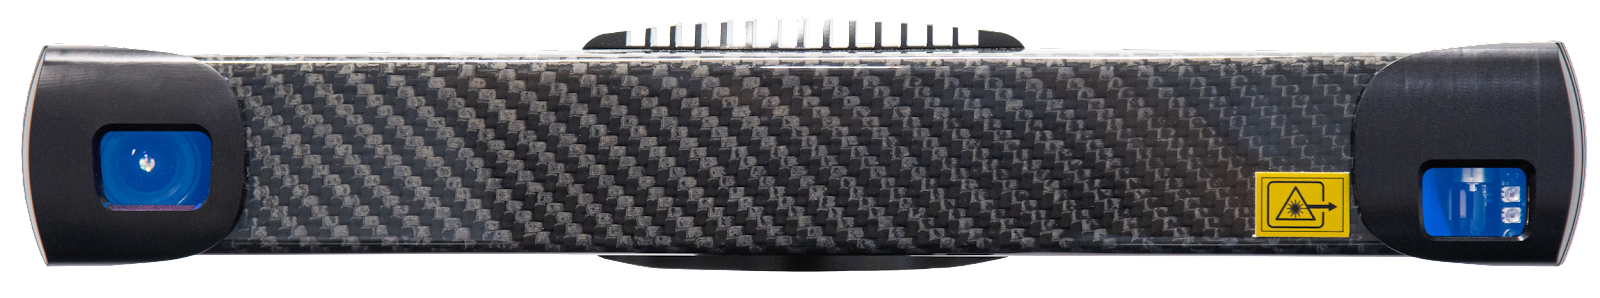
\includegraphics[width=5cm]{Thesis-report/Figures/CAMERA.png}
    \caption{Photoneo Camera [2]}
    \label{fig1.Photoneo Cmaera}
\end{figure}

Using this camera, the camera can capture accurate point clouds and a standard intensity image of the object. Its foundation is a specialized CMOS image sensor that uses Photoneo's patented Parallel Structured Light technology.\\
\begin{figure}[h]
    \centering
    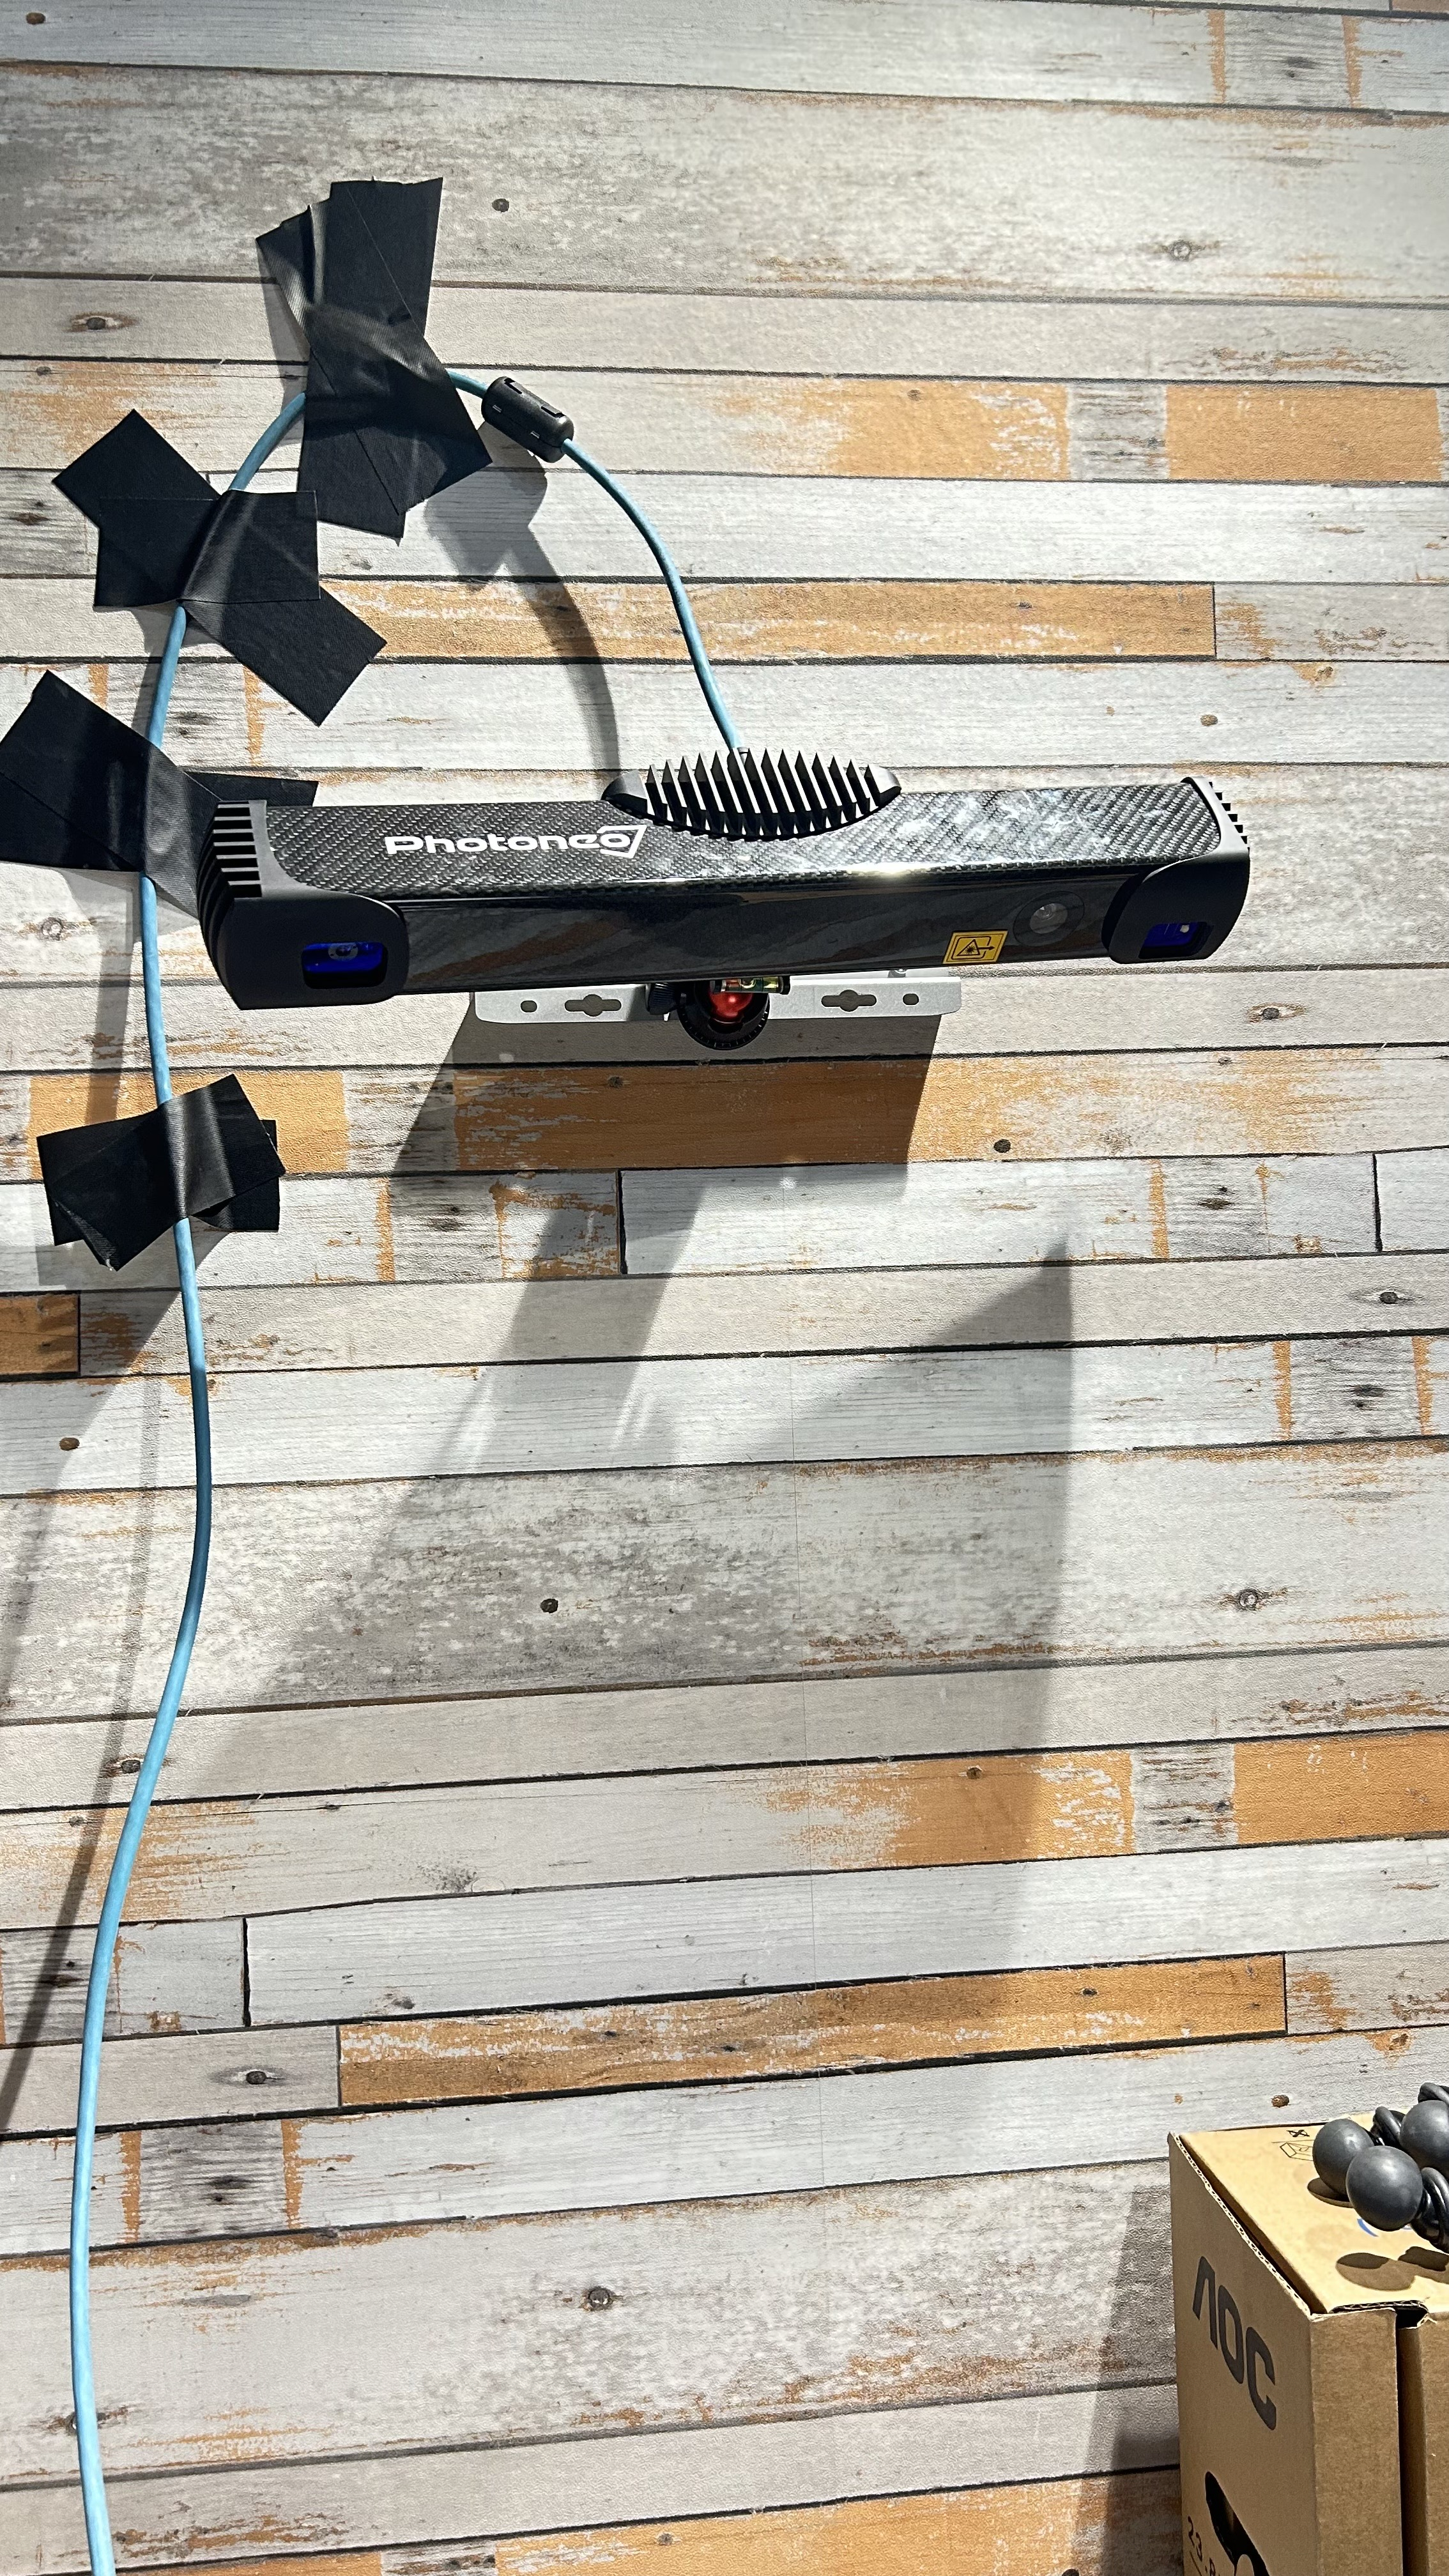
\includegraphics[width=4cm]{Thesis-report/Figures/camera.jpeg}
    \caption{Camera-mounted setup}
    \label{fig1.Photoneo Cmaera}
\end{figure}

To precisely follow the colored area of the RGB marker, we develop and construct a parallel stereo charged-coupled device (CCD) camera system.  Using blob analysis, this ROI was also isolated from the picture live stream and triangulated to determine the 3D coordinates in the world coordinate frame.  Robot path and trajectory planning were assessed using the marker's 3D coordinates, which were converted into the robot frame of reference (robot stereo vision coordinate system).  Therefore, to choose and position an object, our suggested model calculates the real-time distance the robot must travel along the three axes.

The camera's carbon fiber body is lightweight and guarantees the same degree of stiffness as scanners. Three parts comprise the 3D camera: a camera unit with our proprietary Mosaic Shutter CMOS image sensor, a laser projection unit, and a processor unit with a GPU that acts as the brain behind intelligent applications. A sequential structured light, which is utilized in numerous meteorological applications, is the primary technological driver in the first group. One well-suited representative of this category is the 3D scanner range from Photoneo. This technique is not appropriate for dynamic scenes because it uses sequential (multi-frame) capturing. This section is the source of the parallel structured light.\\

\subsubsection{3D Scanning}
The process of 3D scanning involves gathering data from an object's surface and turning it into data points.  These data points are utilized for a digital replication of the scanned object or for a dimension analysis.[17]\\

\subsubsection{Types of 3D scanning}

\subsubsection {Laser Scanning}
Two devices are often used in laser scanning; one directs a laser beam onto a surface, and the other records the precise spot where the object contacts the beam.  Triangulation can be used to calculate the distance between the surface and the scanner and the angle of reflection.[17]\\

\subsubsection {Structure Light Scanning}
This technology projects structured light patterns, such as simple geometric patterns or parallel lines, onto a surface.  The object's shape will cause the patterns to distort.  It is feasible to rebuild the scanned surface by using a camera to analyze these deformations, distinguishing edges, and determining the separation between the item and the scanner.[17]\\

\subsubsection {Photogrammetry}
Triangulation is used in photogrammetry to intersect particular points within two-dimensional images based on the angles at which those points can be found.  To create an acceptable 3D model, a lot depends on the size of the item, the quantity of photos, and their quality.[15]\\

\subsubsection{Time fo Flight}
The time it takes for light to travel from an illumination source to a scene and back is measured by the time of flight. The speed of light itself is the primary obstacle in this situation. Usually, the phase shift of a modulated signal is used to measure time. High pixel modulation frequencies must be used to achieve a respectable level of depth accuracy. The primary drawback in this case is physics, since a greater frequency results in less charge transfer, which lowers contrast and SNR. The restriction suggests an accuracy level that TOF systems can achieve. Usually, it falls within the centimeter range. Another issue is interreflections, which can significantly bend the surface.[15]\\



\subsubsection{Active stereo}
By projecting a synthetic texture onto an object, active stereo addresses the unreliable passive stereo. Nevertheless, it still has to resolve the computationally demanding picture correspondence matching problem. Given the complexity of the matching problem, the projected texture can be either high frequency, which can satisfy a higher resolution but usually has poor reliability, or low frequency, which typically uses random laser dots and can offer higher reliability but poor resolution (the features are sparse).[15]

\subsubsection{Structured patterns/dots}
A spatially encoded pattern is used in structured patterns/dots technology to encode depth disparity information into pattern patches, which are usually projected through a laser diffraction grating in the form of a carefully planned dot collection. The camera must be able to see enough of the patch to reassemble the coding and accurately record the depth information. This produces artifacts on surfaces' edges and tiny objects. The Nyquist-Shannon theorem requires an order of magnitude higher camera resolution to reconstruct individual dots in the projection (and hence 3D measurements). Modern systems use about 25 camera pixels for each 3D measurement, producing about 70k 3D points.[15]

\subsubsection{Parallel Structured Light}
Parallel Structured Light parallelizes the sequential structured light using a sophisticated sensor design, which enables it to record the scene illuminated by various patterns simultaneously. In addition to sharing many of the sequential structured light's benefits, such as resolution and accuracy, it also overcomes one of its main drawbacks: the inability to capture a dynamic environment. Photoneo's Parallel Structured Light gets around the restriction by projecting and capturing numerous encoded patterns. Pixel modulations within our proprietary CMOS sensor are used to accomplish this. Multiple groups of separately modified pixels make up the sensor itself.[15] \\\\ 
\newpage
The Parallel Structured Light's main advantages are:
\begin{enumerate}
 \item  Rapid motion scanning: 40 m/s motion is achieved with a single frame acquisition [15]
\item A more effective depth coding method with accurate, per-pixel measurement that offers ten times greater resolution and accuracy than rival technologies [15]
 \item No motion blur: exposure time of 10 µs per pixel[15]
 \item Quick capture of 1068 x 800 point clouds at 60 frames per second[15]
\item Patent-pending active ambient light rejection technology for outdoor use in direct sunlight[15]
 \item Active rejection of ambient light through interreflection suppression[15]
\item Several devices using the same space at the same time[15]\\

A control unit that operates in tandem with the projection is in charge of these groups. The coded patterns are inserted into the groups rather than changing the projection itself. The sensor may generate over 20 distinct virtual representations of the scene illuminated by the coded patterns injected at the end of the frame. The universal method may be modified on the fly to accommodate various materials and light sources by using any type of pattern typically used for sequential structured light.[15]\\

After undergoing embedded processing, these virtual images are sent via gigabit Ethernet to a client's PC.  Three types of outputs are provided by the sensor:[15]
\begin{enumerate}
    \item Point Cloud: 32 bits per channel  XYZ [15]
    \item 32 bits per channel is the normal map.  XYZ [15]
    \item Texture: Grayscale, 10/12 bits [15]
\end{enumerate}

The sensor produces outputs with a resolution of 1068 x 800 when in "one frame" camera mode.  Approximately 500k individual measurements were used to interpolate these positions.  At a distance of one meter, the usual z-noise standard deviation is less than 0.5 mm (key advantage 1).  Every photon contributes to the 3D measurement in the best possible way thanks to the pixel design.  With sub-pixel accuracy coding (high z-precision) and an efficiency of only 4.5 pixels per 3D measurement, the technology outperforms its competitors and provides the highest XYZ resolution (important benefit 2).[15]\\

The alternative operating mode is a "scanner mode" that is intended for still images.  The sensor provides 1602 × 1200 individual measurements as its raw sensoric output in this mode.  This is recorded in three consecutive frames. A laser that has been deflected by a mirror illuminates the scene.  The projection's 10 µs per pixel exposure may guarantee constant, motion-blur-free data (key benefit 4).[15]\\


\subsubsection{Vision Controller}\\
The figure below shows the vision controller connected to the photoneo camera and the robotic controller using Ethernet (IPV4 address).
\begin{figure}[h]
    \centering
    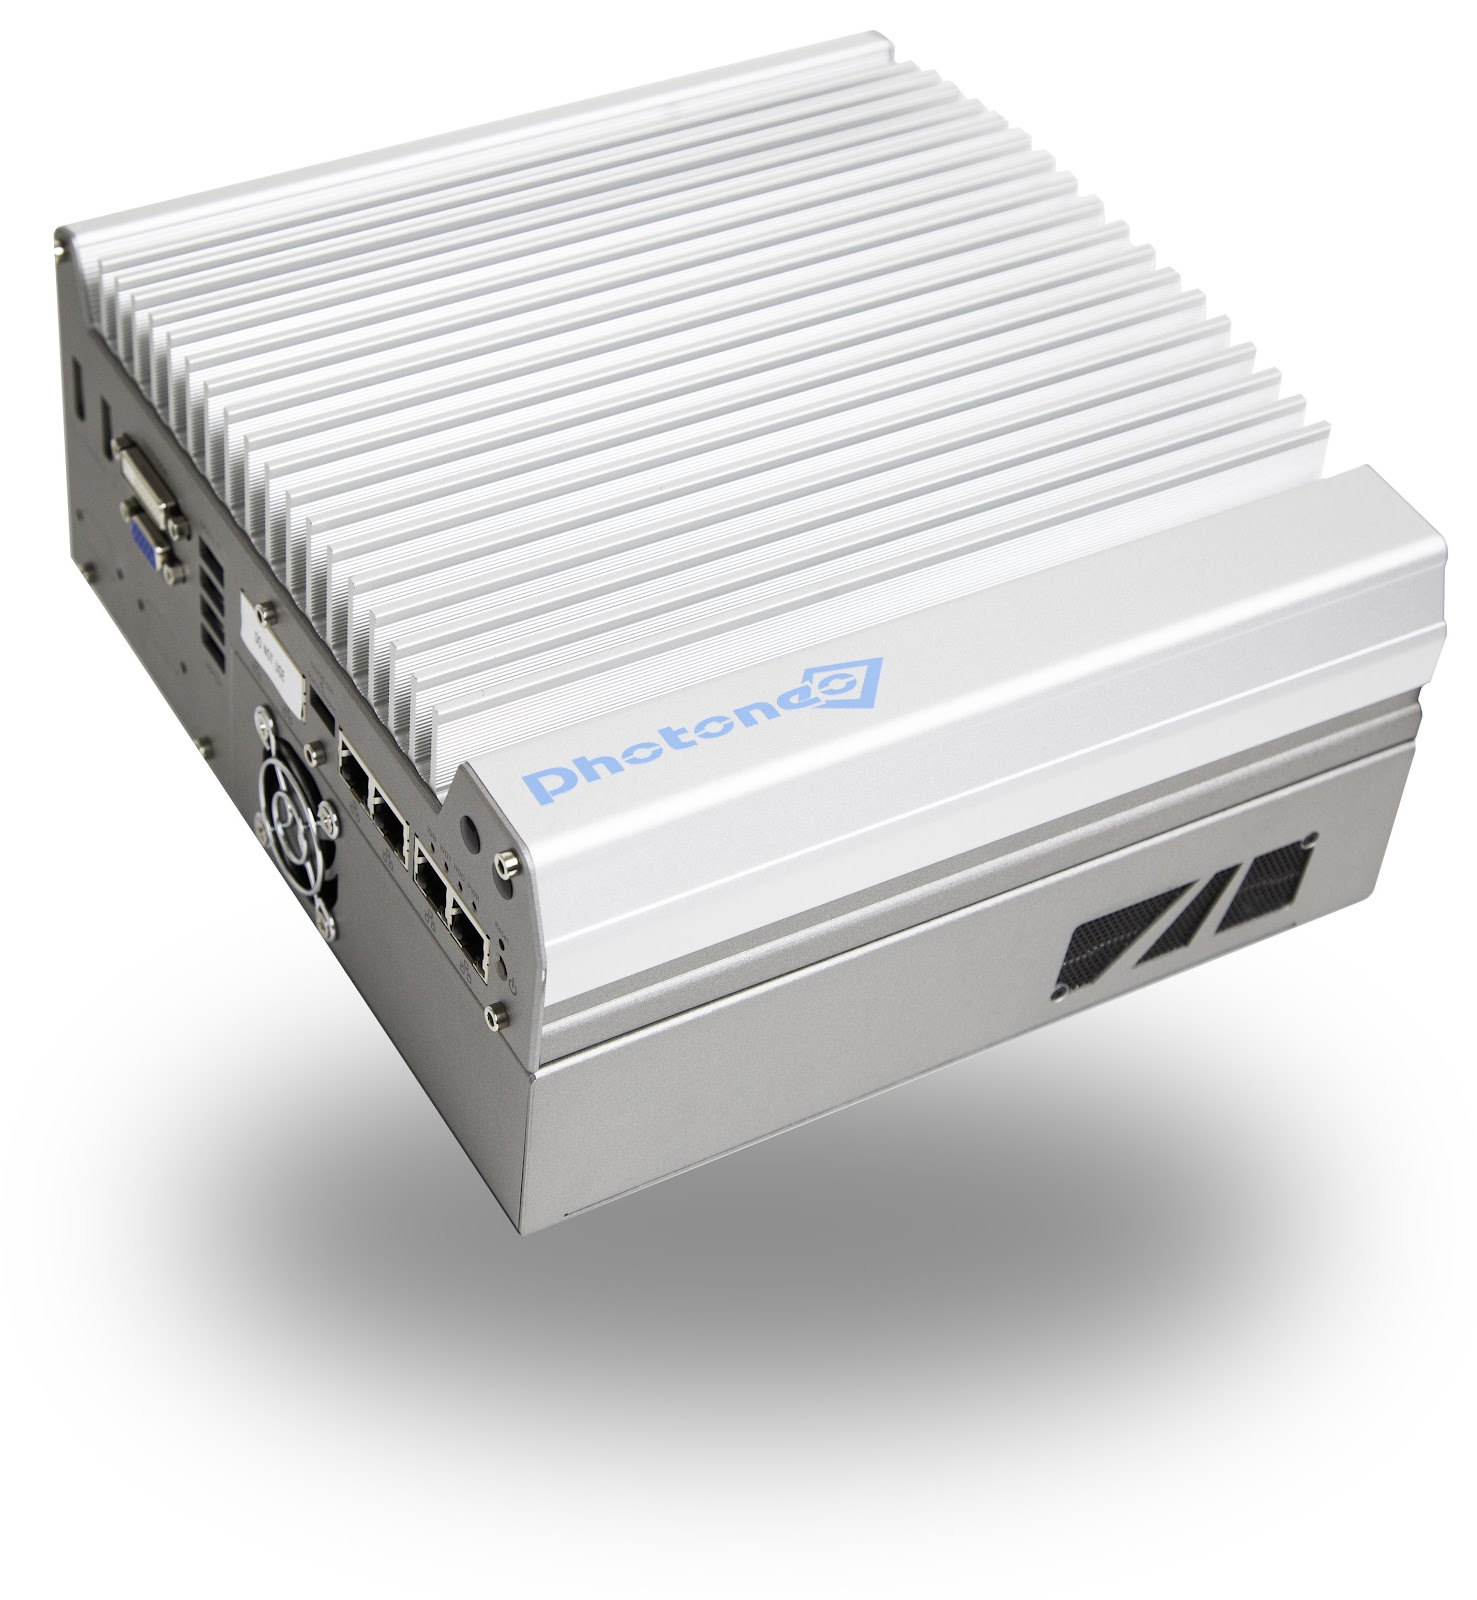
\includegraphics[width=4cm]{Thesis-report/Figures/vision controller.png}
    \caption{Vision Controller[2]}
    \label{fig1.Photoneo Cmaera}
\end{figure}
The vision controller is connected to a PC to get the Web interface to trigger the camera and see the Web interface for communication. Gigabit Ethernet cables (Cat5e or higher) are needed to connect the 3D sensor. A gigabit switch can be used to connect several 3D sensors. The Ethernet connection from the switch or 3D sensor is linked to the scanner's physical network port in both scenarios. To visualize 3D scans, calibrate robot cameras, and establish localization settings, a well-connected connection to the 3D sensor is required.[15]\\
\newpage
To set up the network interface that the vision controller uses to connect to the Photoneo 3D sensor(s), go to the Network page and select the Scanner interface section. Both a fixed IPv6 link-local address and a programmable IPv4 address are features of Photoneo 3D sensors. IPv6 connections are better than IPv4 ones. However, the IPv4 address is used if the IPv6 connection is banned or fails.
\subsubsection{Marker Pattern}\\
\begin{figure}[h]
    \centering
    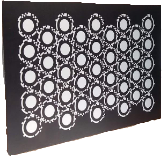
\includegraphics[width=4cm]{Thesis-report/Figures/marker_pattern.png}
    \caption{Marker Pattern[2]}
    \label{fig1.Photoneo Cmaera}
\end{figure}
The figure above shows the S30 calibration board that helps calibrate the conveyor belt, which aligns the coordinates of the object with the conveyor belt for objects passing through the belt. The belt can be used to align the object coordinates with respect to the conveyor belt, so that the robot can pick items from the moving conveyor belt.[2]
\newpage
\subsubsection{Active ambient light rejection:}\\
The inability of all area-based 3D sensors to function in direct sunshine is a typical problem.  Direct sunshine has a maximum power output of 1120 W/m³.  High-end band-pass filters installed in all of Photoneo's sensors lower ambient light levels to around 15 W/m2.  Although it can oversaturate the image or produce high shot noise, this still performs better than the majority of projection systems.
 Delivering active lighting as a brief pulse, which raises the projection's optical power output and shortens the system's exposure time overall, is one way to lessen the impact of ambient light.  This method has drawbacks, such as limited parts availability, complicated power supply management, hazards to eye safety, or problems with heat control.[15]\\

The patent for Photoneo is pending.  The sensor and projection can cooperate to regulate the light sensitivity of the sensor surface through active ambient light suppression.  Only around 1 percent of the sensor surface may be exposed by the direct reflection of the projection at any given point in time during the acquisition due to geometrical constraints.  The remaining 99 percent of the sensor can be turned off by the camera's control circuit, preventing any photoelectrons from being collected.  Scanning in direct sunshine is made possible by the technology's efficient 1:100 suppression of ambient light from any source (key benefit 5).[15]\\

Internal interreflections between pixels are also suppressed by the same technique at the same 1:100 ratio (key benefit 6).  When two sensors are operating in the same space at the same time, the method rejects the projection of the second scanner in 99 percent of the image, with only 1 percent of the pixels impacted.  Easy identification and filtering of these pixels from the output is possible (key benefit 7).[15]
 
\begin{figure}[h]
    \centering
    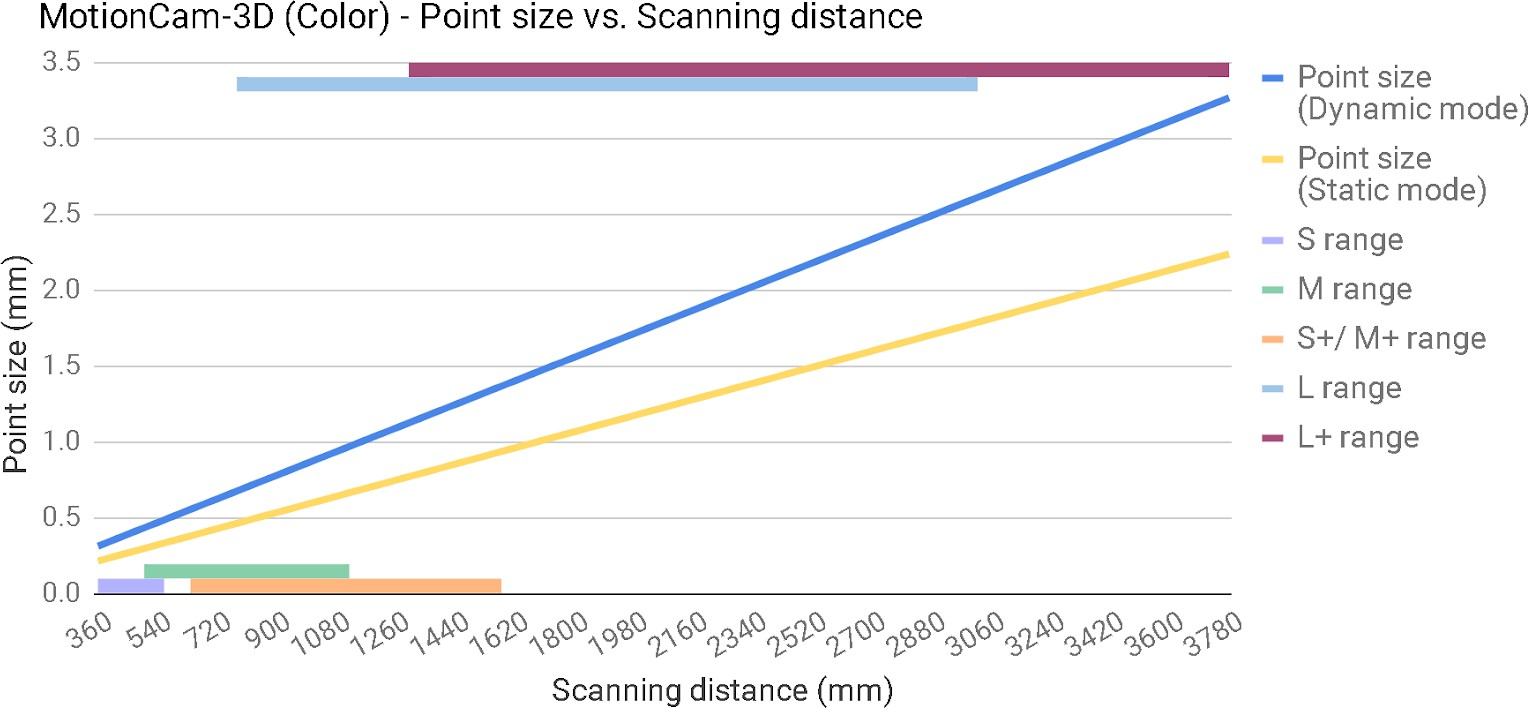
\includegraphics[width=12cm]{Thesis-report/Figures/scanningdistance.jpg}
    \caption{Point size Vs Scanning Distance}
    \label{fig1.Photoneo Cmaera}
\end{figure}\\
\newpage
The figure above shows the scanning distance of various cameras vs their Point size. in this experiment, we have used the M+ Range camera.

\newpage

\newpage
\chapter{\section{\mbox{Literature Review }}{{\normalfont\fontsize{14}{16}\bfseries}}


\newpage
\newpage
\chapter{\section{\mbox{Methodology }}{{\normalfont\fontsize{14}{16}\bfseries}}
This approach uses an interactive route planning solution for a fixed-based manipulator from an initial to a final configuration, along with a camera system for 3D detection.  Two characteristics of the ideal path should be collision-free and metric minimization.\\

Surface imaging and geometry estimation are the two primary subtasks that comprise imaging of the item to be inspected. There are numerous ways to implement automated optical inspection systems in the field of optical inspection.  A good combination of strategies should be chosen based on the task at hand. Improving the contrast between an object's flawed and perfect areas is crucial for dependable and robust automated detection systems in the field of optical surface inspection.  In particular, the lighting and optics define the contrasts.


\label{Literature}
\subsection{Robotic Movement}\\\\
Given a point in the world coordinate, the angle of each joint is calculated based on an inverse kinematics (IK) equation. In general, there may be no analytic IK solution from a manipulator for the configurations of each joint. The numerical method is introduced to solve the problem for
general manipulators. The velocity of the joint can be mapped to Cartesian space with the Jacobian linearization method.\\

\begin{document}

\[
v = J(q) \dot{q}
\]

Pseudo-inverse is used to solve the joint:\\

\begin{document}

\[
\dot{q} = J^\dagger \dot{x}, \quad J^\dagger = (J^T J)^{-1} J^T
\]

Velocity for the linear velocity in Cartesian space. First, FK is used to determine the manipulator's pose. Next, the IK solver uses a pseudo-inverse calculation to update the joint angles. Until the end tip reaches the desired posture with an acceptable error, these two stages are repeated. If the starting value and changing rate are appropriately calibrated, the dynamic gain causes the speed to reach its maximum and minimum quickly. Joint angles have an impact on the inaccuracy during the iteration process. Inappropriate angles cause the gain to drop dynamically, and vice versa.

\subsection{Position of Camera}\\
When mounting a camera for vision operation, it is best to keep it stable and as close to the robot's work envelope as feasible, without interfering with or restricting the movement of the robot arm. The longer the part must travel from the camera's location into the robot's reachable workspace, the more errors the encoder counts will produce, since the accuracy of conveyor tracking with vision depends on the coordinate transformation between the camera's picture-taking location and the robot's work envelope. The camera must be oriented downwards since the components are positioned on the conveyor belt's surface, and vision recognition is done on the parts' upper surface. For the camera's 25 mm lens to cover the entire visible portion of the conveyor belt, a camera fixture was constructed to hold the camera directly above the upstream sensor. The upstream sensor is also used to activate the camera to take a photo when parts are presented at this point, so the picture-taking location is placed at the top of the upstream sensor. Following their placement in fixed locations, the camera and conveyor must be calibrated using the calibration program on the robot controller to configure the camera's properties and determine how the locations of the camera and conveyor relate to the robot's world coordinate.\

\subsection{Camera Examples under different Settings:}\\
The below figures show the examples for the object taken under the camera settings:\\


\textbf{1.Texture:}
The texture helps in ensuring the details of the object look natural. Moreover, it helps in being visually understandable.
    \begin{figure}[h]
    \centering
    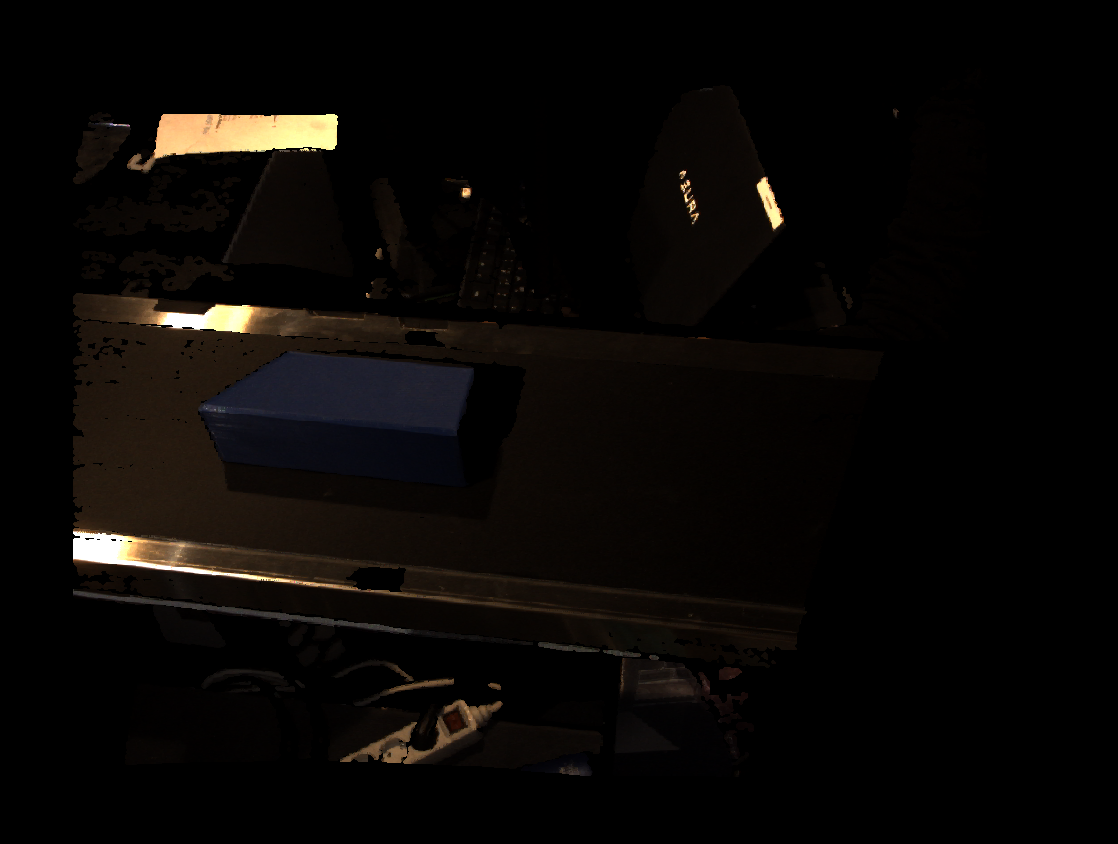
\includegraphics[width=6cm]{Thesis-report/Figures/new_Texture.png}
    \caption{Texture}
    \label{fig1.Photoneo Cmaera}
\end{figure}\\
\textbf{2.EventMap:}
The Event Map helps in capturing objects in fast motion without any blur.It helps in capturing the full frames at a fixed rate.
    \begin{figure}[h]
    \centering
    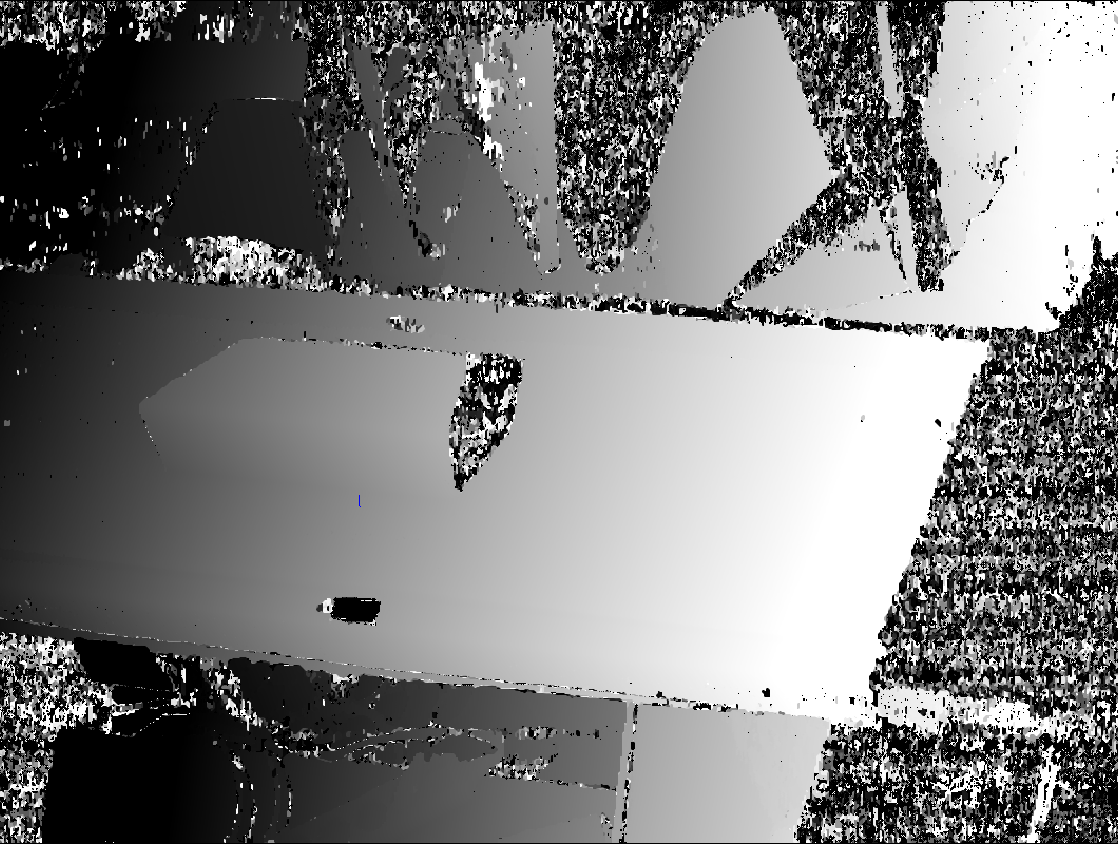
\includegraphics[width=6cm]{Thesis-report/Figures/new_EventMap.png}
    \caption{EventMap}
    \label{fig1.Photoneo Cmaera}
\end{figure}\\

\textbf{3.DepthMap Grayscale}
The DepthMap grayscale is needed as it explains in storing the complex 3D coordinates, where it consists of Brighter pixels and Darker pixels.
    \begin{figure}[h]
    \centering
    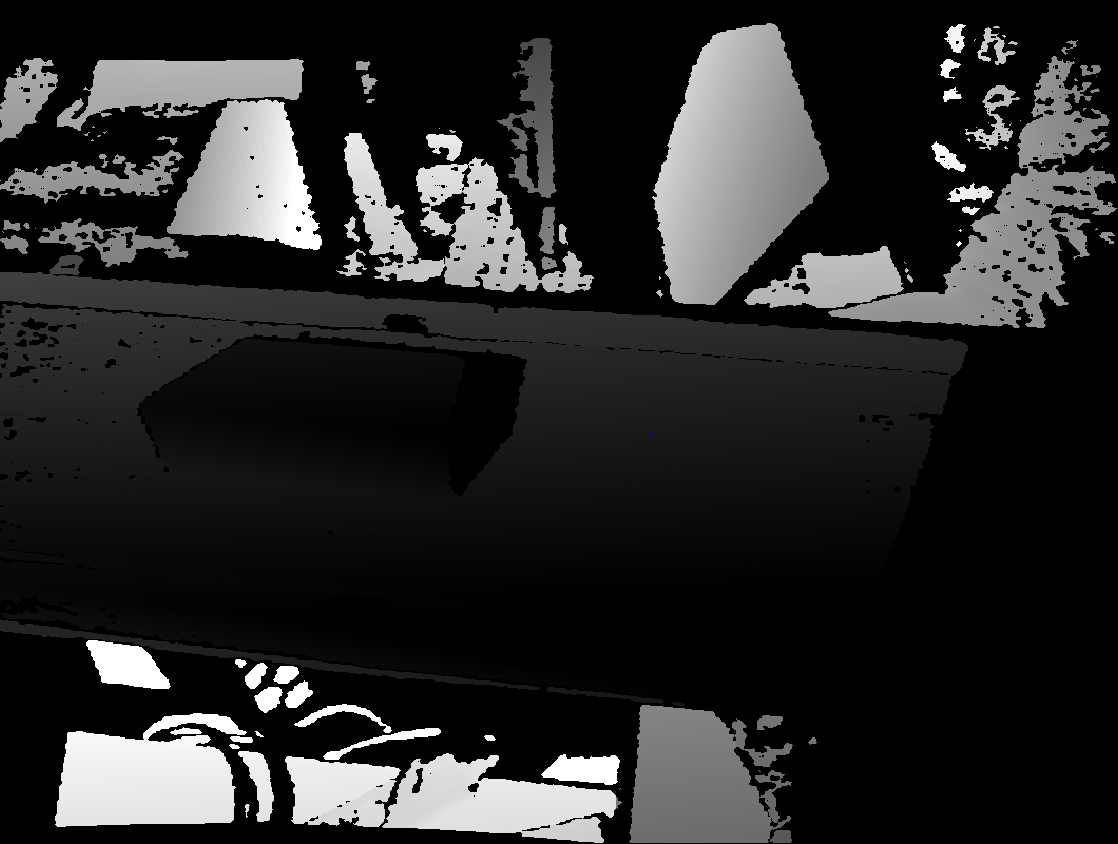
\includegraphics[width=6cm]{Thesis-report/Figures/new_DepthMap.png}
    \caption{DepthMap Grayscale}
    \label{fig1.Photoneo Cmaera}
\end{figure}\\
\textbf{4.Depth Hue:}
The Depth Hue is needed as it is a more intuitive and visually distinct way to represent the depth as compared to the grayscale depth map.
    \begin{figure}[h]
    \centering
    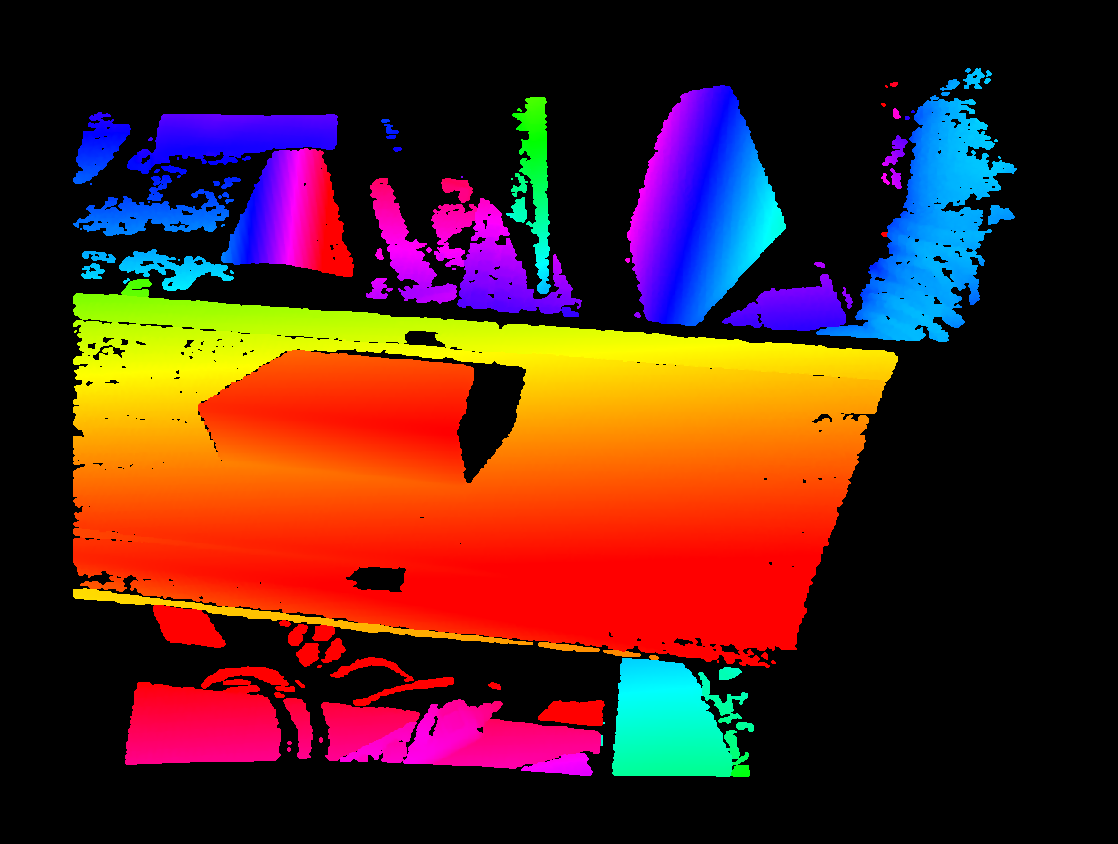
\includegraphics[width=6cm]{Thesis-report/Figures/new_Depth_Hue.png}
    \caption{Depth Hue}
    \label{fig1.Photoneo Camera}
\end{figure}\\
\textbf{5.Confidence Map:}
It is needed to indicate the reliability of depth or image data. It helps in filtering the Noisy and unreliable data.
    \begin{figure}[h]
    \centering
    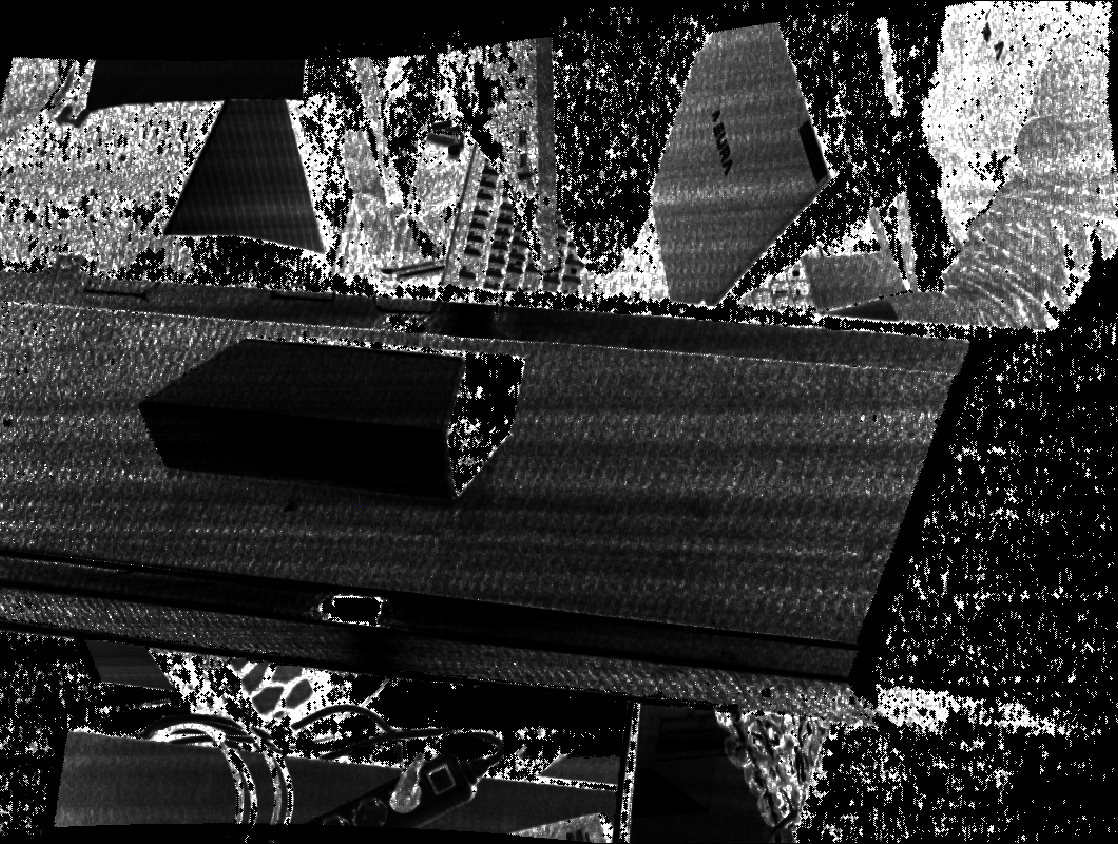
\includegraphics[width=6cm]{Thesis-report/Figures/new_ConfidenceMap.png}
    \caption{Confidence Map}
    \label{fig1.Photoneo Cmaera}
\end{figure}\\
    \begin{figure}[h]
    \centering
    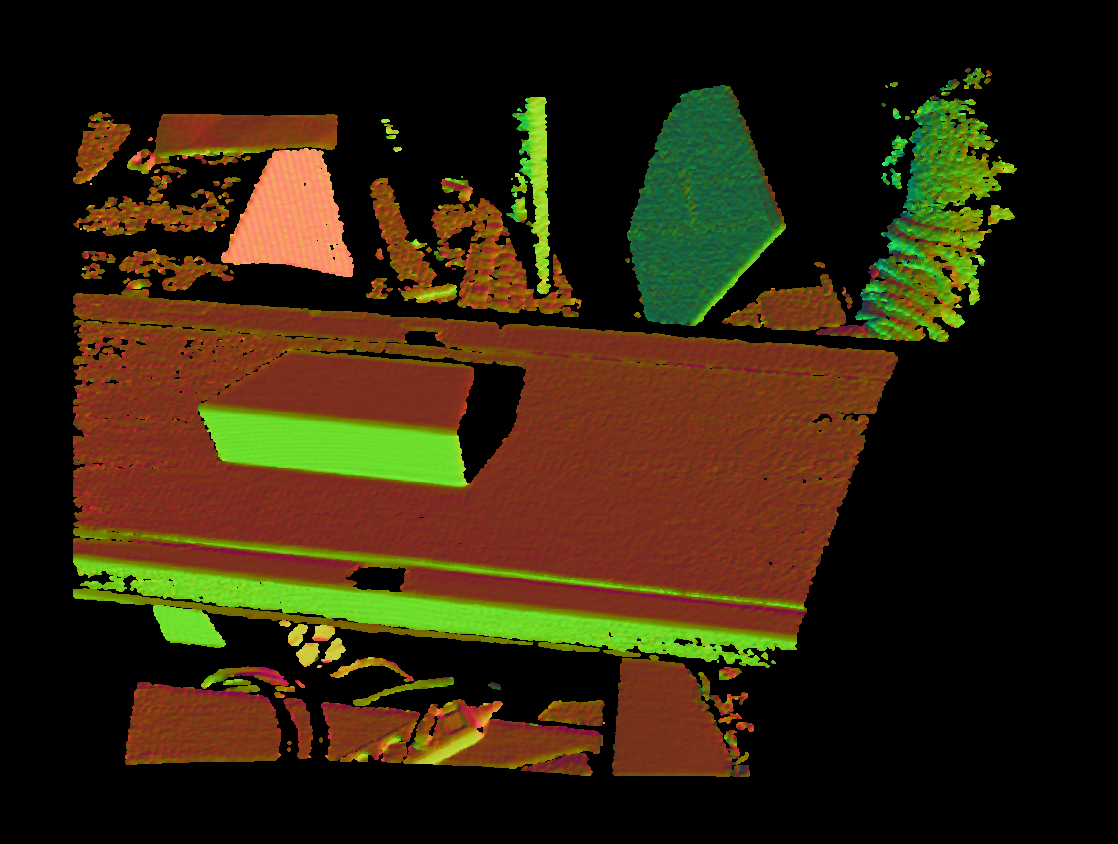
\includegraphics[width=6cm]{Thesis-report/Figures/new_Normals.png}
    \caption{Normals}
    \label{fig1.Photoneo Cmaera}
\end{figure}\\
\textbf{6.Normals:}
The normals are defined, and how they interact with the light and other physical effects. They are very much needed for realistic rendering, depth understanding in computer vision, and graphics.

\textbf{7.White}
    \begin{figure}[h]
    \centering
    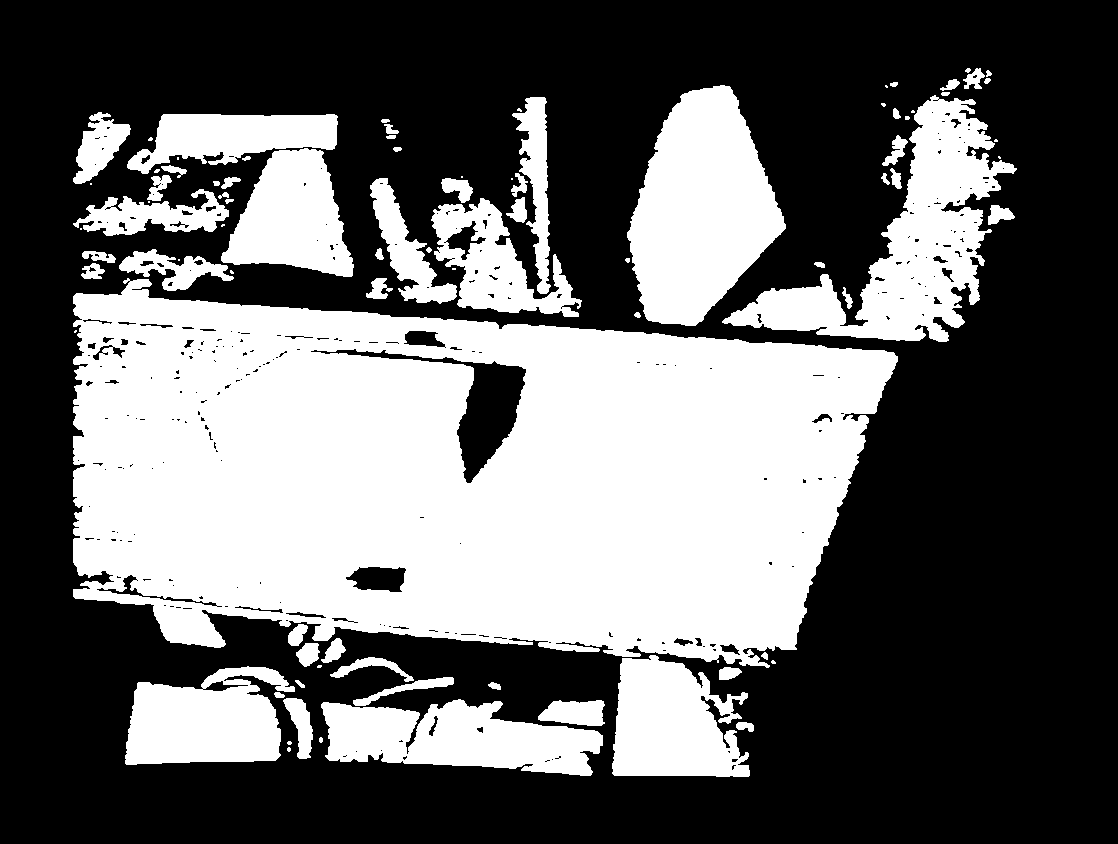
\includegraphics[width=6cm]{Thesis-report/Figures/new_white.png}
    \caption{White}
    \label{fig1.Photoneo Cmaera}
\end{figure}\\
\textbf{8.Color Image:}
It provides the visual information, making object recognition, segmentation, and realistic rendering in computer vision, image generation, etc.
    \begin{figure}[h]
    \centering
    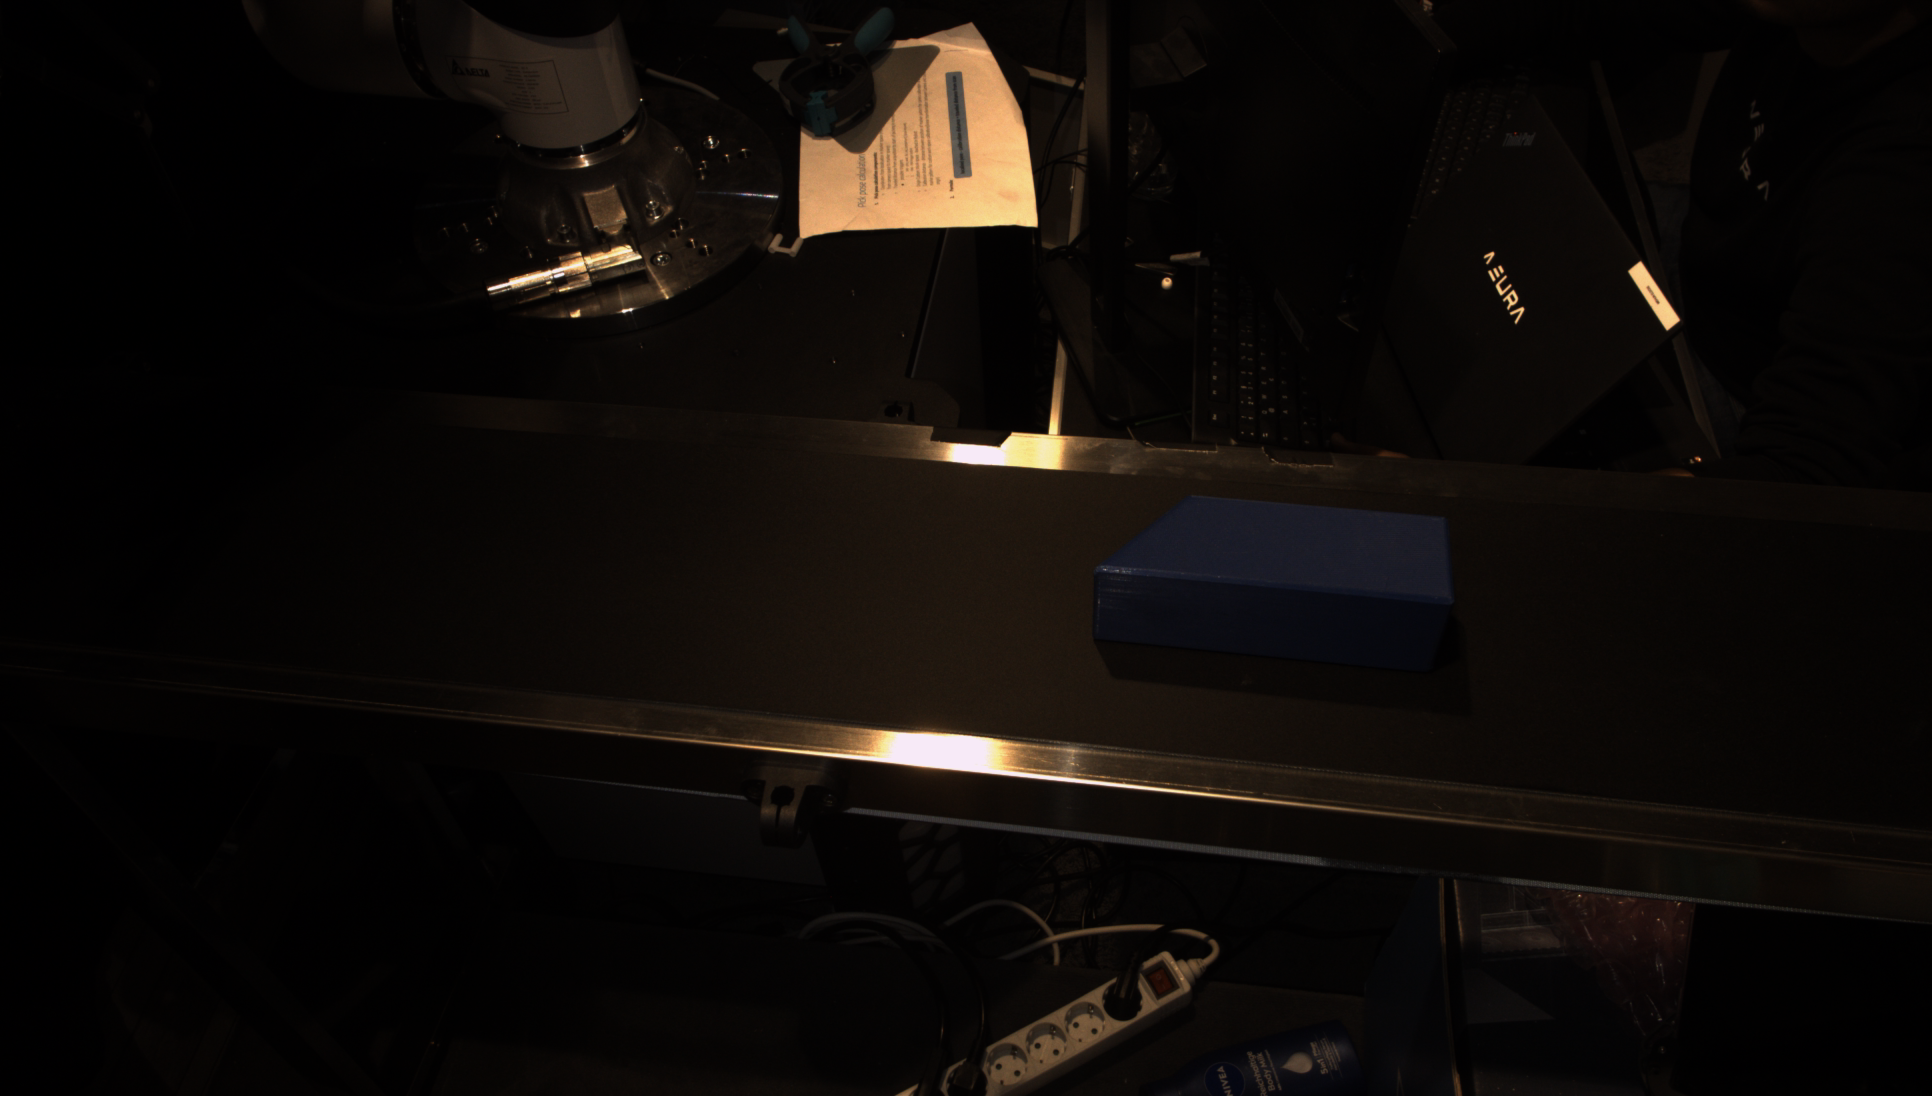
\includegraphics[width=6cm]{Thesis-report/Figures/new_white_IMG_ColorCameraImage_8Bit.png}
    \caption{Color Image}
    \label{fig1.Photoneo Cmaera}
\end{figure}\\

\subsection{Object Identification}\\
\begin{figure}[h]
    \centering
    \includegraphics[width=8cm]{Thesis-report/Figures/Trapezoid web.jpeg}
    \caption{Object Identification in Web interface}
    \label{fig1.Photoneo Cmaera}
\end{figure}

The STL file is uploaded to the Web interface, thereby helping the camera to identify the object in the moving conveyor belt tracking system. Once the object is detected, the camera helps in getting the object's position and its quaternion values.

 \newpage
\subsection{Trajectory Planning}\\
Using a set of predetermined points, trajectory planning aims to produce stable and fluid motion in world coordinates. A few characteristics, such as the maximum velocity, acceleration, and jerk, will be taken into account to demonstrate the continuous motion of the robot arm. The constant context of temporal movement is unique. Additionally, this function has a first derivative and a second derivative. In addition to increasing wear on the mechanism, jerky action frequently causes vibration in the robot manipulator.\\
The fundamental path interpolation functions, such as linear and point-to-point movement, are carried out when the precondition parameters have been addressed. Interpolation, which is determined by previous factors, will produce the path segments. A self-defined function is crucial to the creation of path segments in Cartesian space. Joint command and linear command can both follow the point-to-point movement. Every joint's present condition is indicated in the joint space.\\

\begin{figure}[h]
    \centering
    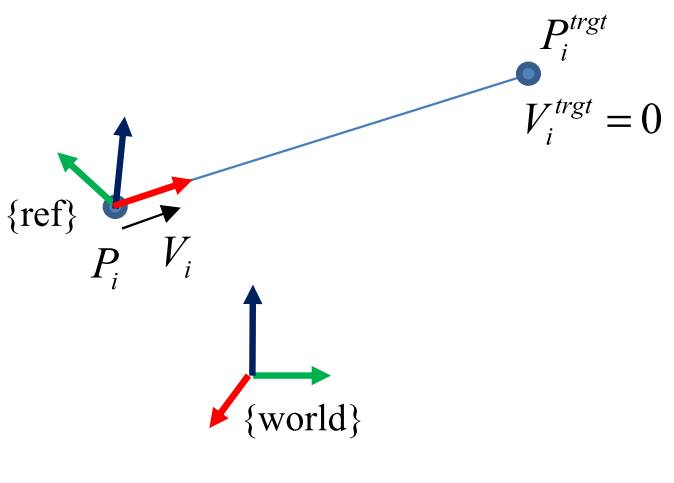
\includegraphics[width=5cm]{Thesis-report/Figures/new.png}
    \caption{Coordinate system}
    \label{fig1.Photoneo Cmaera}
\end{figure}

All joints will arrive simultaneously before approaching targets since the velocity is zero at the target point. In contrast to point-to-point motion, linear movement at the end-effector makes it easy to demonstrate the condition from the reference coordinate. The motion will only be linked to one DoF during variation if the current velocity point toward the target position is specified. To execute gripping operations, the robot arm will thereafter alter its motion via path segments. Manipulators can grab a stationary workpiece with the aid of trajectory planning and object recognition algorithms.

The fundamental path interpolation functions, such as linear and point-to-point movement, are carried out when the precondition parameters have been addressed. Interpolation, which is determined by previous factors, will produce the path segments. 
\subsection{Traking Method}\\
In the preceding part, the picking procedure was put into practice. With some dynamic adjustments, the situation is now more challenging. The robot should be updated with the object's information when it begins to move on the conveyor to use the tracing talent. The tracking technique presents certain difficulties when using a visual control system. First, we must use real-time frame-by-frame image processing to track the objects. Next, we use the average of the previous ten frames as a guide. Second, we must specify the gripper's position about the moving object. We came up with one method for determining the objects' positions. Kinects that can recognize objects can also provide us with depth information in addition to the target's color. Next, using the information gathered, we devise a method to obtain 3D coordinates and calibrate the scale to the y and z-axes while taking into account the depth frame, which is the x-axis under Kinect view. Finally, the robot's reaction will complete the grabbing maneuver by following the updated data. Our tracking strategy is divided into three subsections. \\ 

By calibrating the y and z axes, we may create a prospective viewpoint to enhance object location after obtaining the past 10 frames as a reference to compare with the present frame. The tracker would ultimately follow the target by the predicted trajectory after we had the position of the tracker and the target.\\\\
Initially obtain the tracker's (gripper) and the target's (workpiece) instantaneous positions independently once the camera has determined the outlines of objects. First, the contour is the difference between the color frame and the reference and current frames. The coordinates of the items in the depth frame are then obtained. The situation along the x and z axes in the depth frame and the y and z axes from the Kinect color frame are among the desired data. \\
\newpage
The tracker and target belong to different x-y planes; thus, we may utilize a threshold regarding the data along the z-axis in the color frame in Kinect view to separate the objects. It is referred to as the robot palm if the coordinate along the z-axis is more than the threshold.
\subsection{Position Calibration}\\
Static pose recognition will end when the tracking approach is activated. The end-effector and object positions on the conveyor are among the data. The workpiece will proceed through the conveyor in a straight line. Therefore, only the workpieces' positions will be changed, and their orientation will remain unchanged. It is important to note that the end-effector might follow the subsequent instructions based on the tracking approach. This doesn't assist with grabbing articles, though. The gripper should take aim-off into account when doing object tracking to ensure that the entire gripping process is complete. Thus, proper gripping position by the tracking method turns out to be an important point. Without additional indication, the arm might not be aware of some issues that arise on the conveyor.

\subsection{Encoder offsets}\\
The main method for defining robot movements about a conveyor belt is to model the belt using a unique kind of position data called belt variables. The position of a reference frame fixed to the moving belt conveyor is defined by a belt variable, which is regarded as a relative transformation with a component variable in time. The relationship between a belt encoder and the position and speed of the reference frame, which keeps a fixed position and orientation concerning the belt, can be described using such a belt variable. A belt variable is defined as:

\[
\text{DEFBELT} \, \% \text{belt-variable} = \text{nominal-trans}, \, \text{scale factor}
\]
Where scale factor is a calibrating constant that specifies the ratio between the elementary displacement of the belt and one pulse of the encoder; nominal-trans is the value in R6 of the (simple or composed) relative transformation that defines the position and orientation of the conveyor belt; and belt-variable is the name of the belt variable to be defined. The nominal transformation specifies a position (X, Y, Z) that points to the approximate center of the belt concerning the robot's base frame; the X axis of the nominal transformation indicates the direction of motion of the belt; and the XY plane defined by this transformation is parallel to the conveyor belt surface.\\
\[
\text{XYZ-instantaneous} =
\text{XYZ-nominal} + \text{belt-distance} \cdot \text{vers}(X_{l,\sim,\text{minal\_rrarrv}})
\]

\[
\text{with} \quad \text{belt-distance} =
(\text{encoder-count} - \text{encoder-offset}) \cdot \text{scale-factor}
\]
Where encoder-count is the encoder's read contents, and encoder-offset is used to determine the belt's reference frame's instantaneous location (x, y) about its nominal location (x, y). Specifically, a displacement carried out by the conveyor can be nullified by using the offset of the belt (by setting the offset value to the current value of the encoder's counter). The conveyor's visual robot tracking system takes into consideration fluctuating belt offsets, which are often altered by software operations.
\[
\text{SETBELT} \ \% \text{belt-variable} = \text{expression}
\]

For picking-on-the-fly robot tasks, a fast digital-input interdigital input that detects the occurrence of an external event of the type "an object has completely entered the conveyor belt window" (and hence is completely visible) will initiate the dynamic robot-vision synchronization based on the "look-and-move" cooperation principle. A photocell detects this event and uses it to determine whether to take an image of the moving item.
\subsection{Moving Calibration through Conveyor belt}\\
The trajectory follows the instructions produced from trajectory planning and eye-in-hand vision each time the robot arm's palm begins to perform a moving task. The border of the conveyor will show up on the top side of the image when viewed through a camera. Because the conveyor's moving path is linear, the robot's motion can be corrected by following the conveyor's edge slope. The line equation in polar coordinates is used to determine the conveyor's line edge. The polar parametric form has the advantage of having no singular condition in the domain of sinusoidal functions.

\begin{equation}
r = x\cos\theta + y\sin\theta
\end{equation}

\subsection{Transformation of Coordinates:}\\
To enable the robotic arm to know where to pick and position the target objects, the primary objective of the object coordinate transformations is to convert the target objects' coordinates from the image plane coordinates to the robot base coordinates.[3]
 The pinhole camera model and the chain of transformations for the robotic system with eye-to-hand configuration are combined to create the chain of coordinate transformations for a robotic system with eye-to-hand configuration.[3]\\

\[
\text{camP}_{\text{obj}} = C_Z \cdot K^{-1} \cdot p_{\text{obj}} [3]
\]

where: cam  Pobj: [u, v, 1]" on the image plane; Pobj: The object point [EX, CY, CZ]" in the camera frame.
 The calibration of the eye-to-hand stereo camera yields the intrinsic matrix K in above Equation (4), and the estimation of depth based on the disparity is used to determine the depth ° Z.
 The coordinate conversion from the stereo camera frame to the robot base frame is the second operation sequence.  The transformation matrix base Heam, which is determined from the eye-to-hand calibration, is used to do this.  Combining the first and second operation sequences yields the equation:\\

 \[
\text{baseP}_{\text{obj}} = {}^{\text{base}}H_{\text{cam}} \cdot \text{camP}_{\text{obj}} [3]
\]

where: base Pobj: The robot base frame's object point; base  Heam: The matrix used to convert the robot base frame from the stereo camera frame.Finally, the above two equations are combined to give the overall transformation equation for the entire system .For a robotic system with an eye-to-hand arrangement, the equation below shows the series of coordinate transformations from the image plane to the robot base frame.[3]\\

 \[
\text{baseP}_{\text{obj}} = {}^{\text{base}}H_{\text{cam}} \cdot \text{camP}_{\text{obj}} [3]
\] 

\\

 \[
\text{baseP}_{\text{obj}} = {}^{\text{base}}H_{\text{cam}} \cdot \left( C_Z \cdot K^{-1} \cdot p_{\text{obj}} \right) [3]
\]


\subsection{Software Codes}
\subsubsection{Servo-X}
The servoX is the motion of the robot in Cartesian space, where we need to define the max velocity, max acceleration, and its servoX proportional gain. Initially, the coordinates that we get from the camera space as Quaternion values that include [X, Y, Z, ex, ey,ez] as the target values for the robot to move to that particular position and pick up the object. Since we have a calibrated camera concerning the Robot frame, the coordinates that we get from the object will be concerning the robot frame.
\subsubsection{Move Linear:}\\
The above method is basically used in the dynamic application, where the object coordinates(Quaternion values) [X, Y, Z, Ex, Ey, Ez] these values are passed to the robot controller directly for moving to the target position. Here we need to provide the max acceleration, max velocity for the robotic movement.

\subsection{Calibration for camera for Workspace}\\\\

Go to the Calibration page within the solution to begin the calibration.  The following details are displayed along with a list of all defined vision systems: [2]
\begin{enumerate}
    \item ● ID: the Vision system's ID[2]
    \item ● Name: the Vision system's name [2]
    \item ● Scanner ID: the ID of the 3D sensor used by the Vision system [2]
    \item ● Scanner status: the current state of the 3D sensor used by the Vision system[2]
    \item ● Scanner model: the model of the 3D sensor used by the Vision system [2]
    \item ● Calibration type: the type of calibration based on the selected 3D sensor mount position [2]
    \item ● Calibrated: whether the Vision system has already been calibrated[2]
    \item ● Accuracy of calibration [mm]: the precision of any prior calibration   [2] 
\end{enumerate}

\begin{figure}[h]
    \centering
    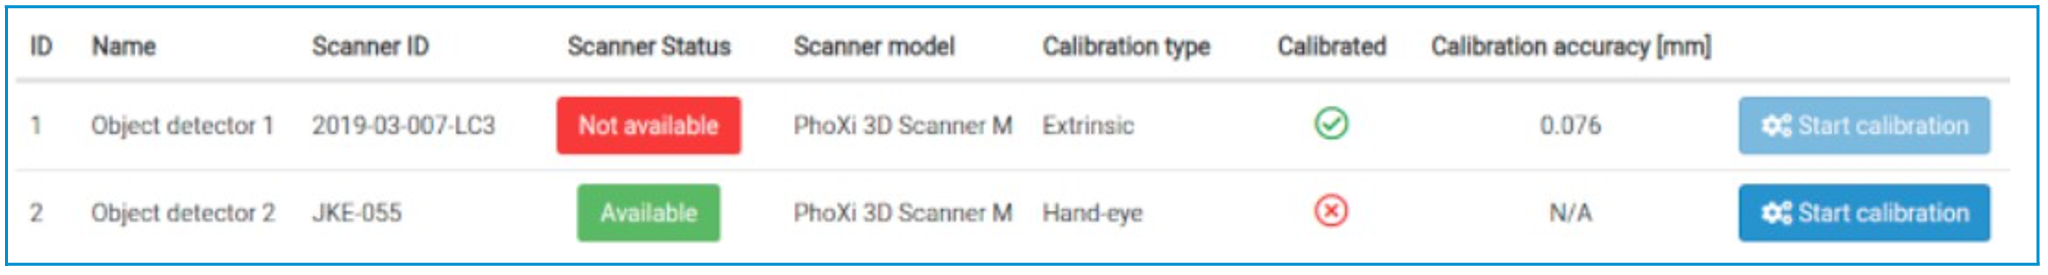
\includegraphics[width=13.5cm]{Thesis-report/Figures/calib.png}
    \caption{Calibration [2] }
    \label{fig1.Photoneo Cmaera}
\end{figure}
The camera calibration is performed through an extrinsic method in which the camera is fixed in a position and the calibration ball is fixed at the end of the robot TCP.\\
\begin{figure}[h]
    \centering
    \includegraphics[width=12cm]{Thesis-report/Figures/calibration.jpeg}
    \caption{Calibration for camera with respect to Robot frame [2] } 
    \label{fig1.Photoneo Cmaera}
\end{figure}
The below figure shows how the calibration is happening by adding the point by fixing the point where the robot Coordinates [X, Y, Z] rotation values will save the points by saving the points (represented as a green point). Here, we need to add 9 points to get the calibration workspace. After the calibration, the average value from the 9 points is taken into consideration.(The lesser the value better the accuracy) [2]\\ 

The below figure shows the calibration method used in this study (Extrinsic Calibration) (EC), where the camera is fixed at the location, and 9 points are taken into consideration, where the average value is finally taken as the value for the calibration. [2]\\

This kind of calibration is employed in configurations where the 3D sensor is fixedly positioned within the robotic cell, often above the bin. The 3D sensor does not have to be stationary concerning the robotic cell itself; it just needs to be stationary concerning the robot's foundation.[2]
\begin{figure}[h]
    \centering
    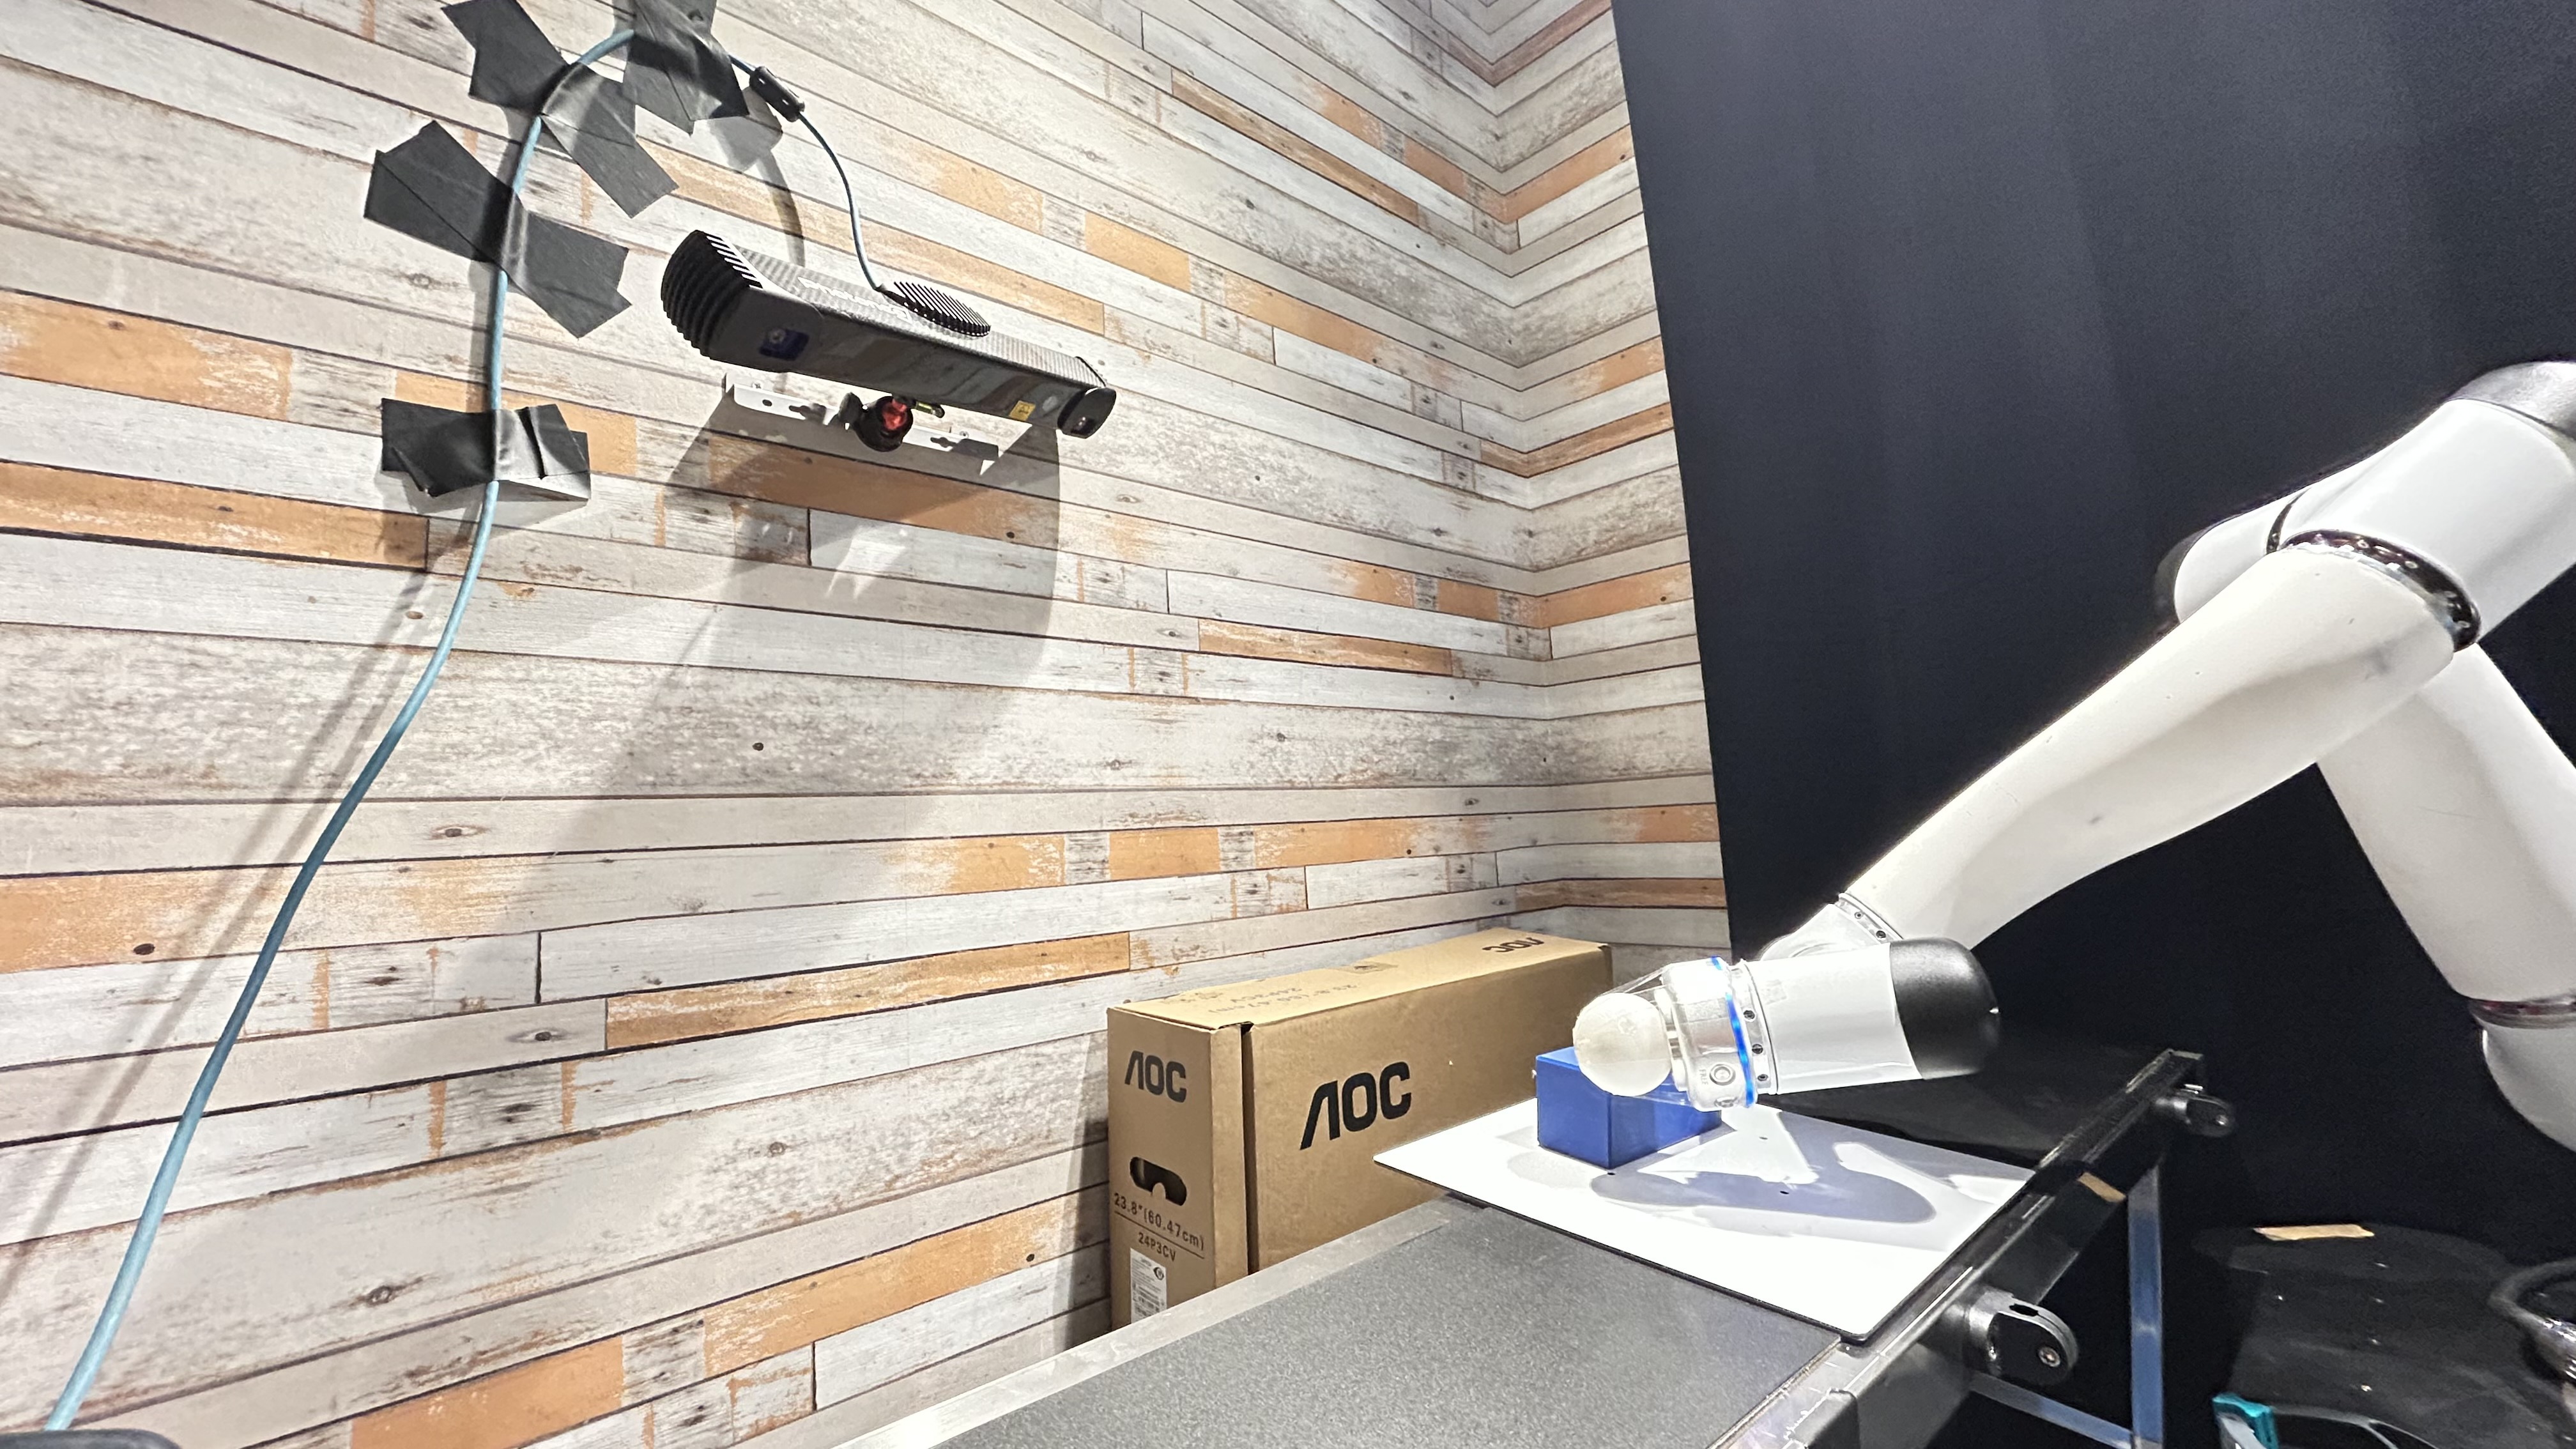
\includegraphics[width=10cm]{Thesis-report/Figures/extrinsic_ball.jpeg}
    \caption{Calibration for the camera concerning the Robot frame}
    \label{fig1.Photoneo Cmaera}
\end{figure}
Finding a camera's intrinsic matrix, extrinsic matrix, and distortion coefficients is the aim of camera calibration. The relationship between the camera frame and the chessboard frame is described by the extrinsic matrix, whereas the relationship between the picture plane and the camera frame is described by the intrinsic matrix. Hand-eye calibration aims to establish the transformation relationship between the cameras and the robotic arm.  The location of an object in the camera frame can be converted into its location in the robot base frame once the transformation connection has been established. The robotic arm will then be able to locate the object and pick it up. Finding the transformation matrix between the robot base and the camera (base H cam) is the aim of an eye-to-hand calibration.[3]\\

 \[
{}^{cam}\!H_{cal} = {}^{cam}\!H_{base} \cdot \left( {}^{base}\!H_{tcp} \cdot {}^{tcp}\!H_{cal} \right) = {}^{cam}\!H_{base} \cdot {}^{base}\!H_{cal} [3]
\]

The transformation matrix in the above equation that must be computed for the eye-to-hand calibration is cam H base.  Cam H cal, which can be computed using either 3D recognition of the calibration rig or camera calibration (extrinsic matrix), is the transformation matrix from the calibration rig frame to the camera frame.  Forward kinematics can be used to calculate base H cal, the transformation matrix from the calibration rig frame to the robot base frame.
\\ The calibration matrix will become invalid, and the entire calibration process will need to be restarted if there is a change in the relative position between the 3D sensor and the robot after the calibration. In other words, after the system has been calibrated, the 3D sensor cannot be changed concerning the robot.[3]\\


\begin{figure}[h]
    \centering
    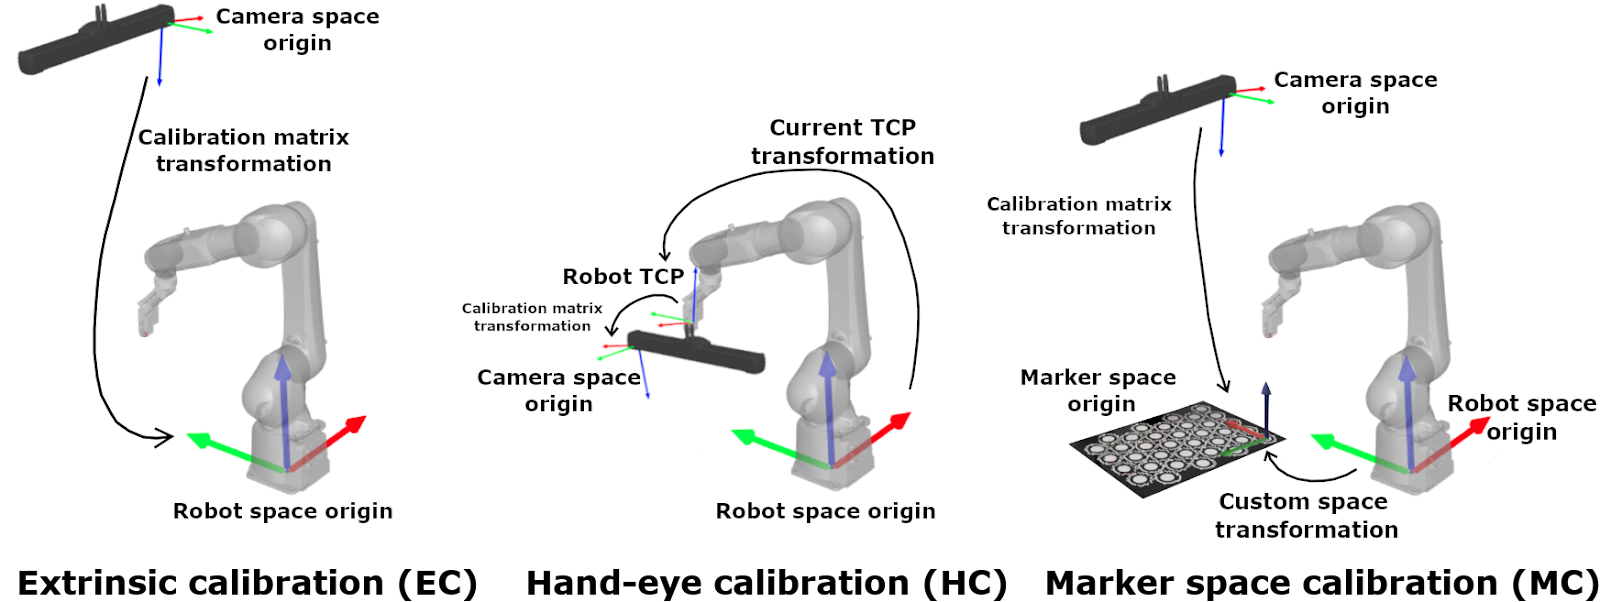
\includegraphics[width=13cm]{Thesis-report/Figures/extrinsic.png}
    \caption{Extrinsic Calibration [2] } 
    \label{fig1.Photoneo Cmaera}
\end{figure}

The calibration matrix specifies the transformation straight to the robot base coordinate system because the 3D sensor is fixed. With this configuration, the robot's mobility is unrestricted, and it doesn't need to halt during the scan acquisition, unlike with the hand-eye approach.[2]


\subsubsection{Calibration Ball}\\\\


A calibration ball serves as the calibration object. It is also feasible to use a bespoke ball with the right characteristics in place of the calibration ball, the ball needs to be exactly round and composed of a surface that is good for scanning (smooth and not extremely reflective). The ball needs to be attached to the gripper or the flange, which are the robot's endpoints. During the calibration process, make sure the ball is securely attached and stays in place. Verify that the ball can be seen clearly by the 3D sensor.[2] \\
\begin{figure}[h]
    \centering
    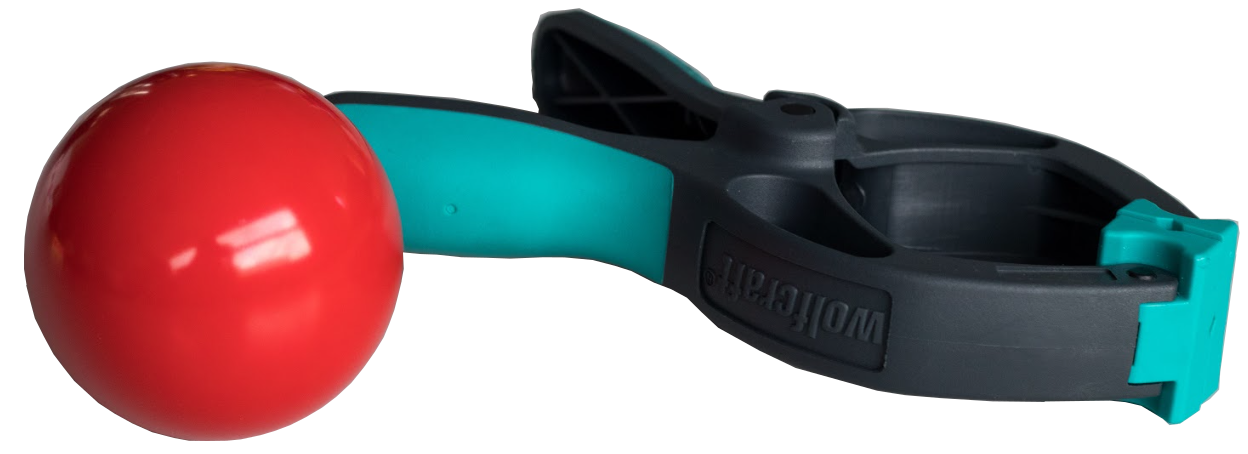
\includegraphics[width=5cm]{Thesis-report/Figures/ball.png}
    \caption{Callibration ball [2] }
    \label{fig1.Photoneo Cmaera}
\end{figure} 


The following components make up the calibration interface:
\begin{enumerate}
    \item  ● Visualization: You can alternate between the Texture and Verification tabs. ● Texture image (Texture tab)
 The last scan acquisition produced the texture image.
 If the localized calibration ball was successfully located for the extrinsic calibration, it is indicated with a green highlight.  On the other hand, that portion of the texture will be highlighted in red if there is insufficient ball surface visible or if another item with a similar shape is found.[2]
 \item  ● 3D visualizer (Verification tab) 
The visualizer shows the point cloud and 3D sensors from all vision systems.
 The following items appear once the necessary number of calibration points has been added: [2]
\item ● Add calibration point: a button for manually adding a calibration point [2]
\begin{figure}[h]
    \centering
    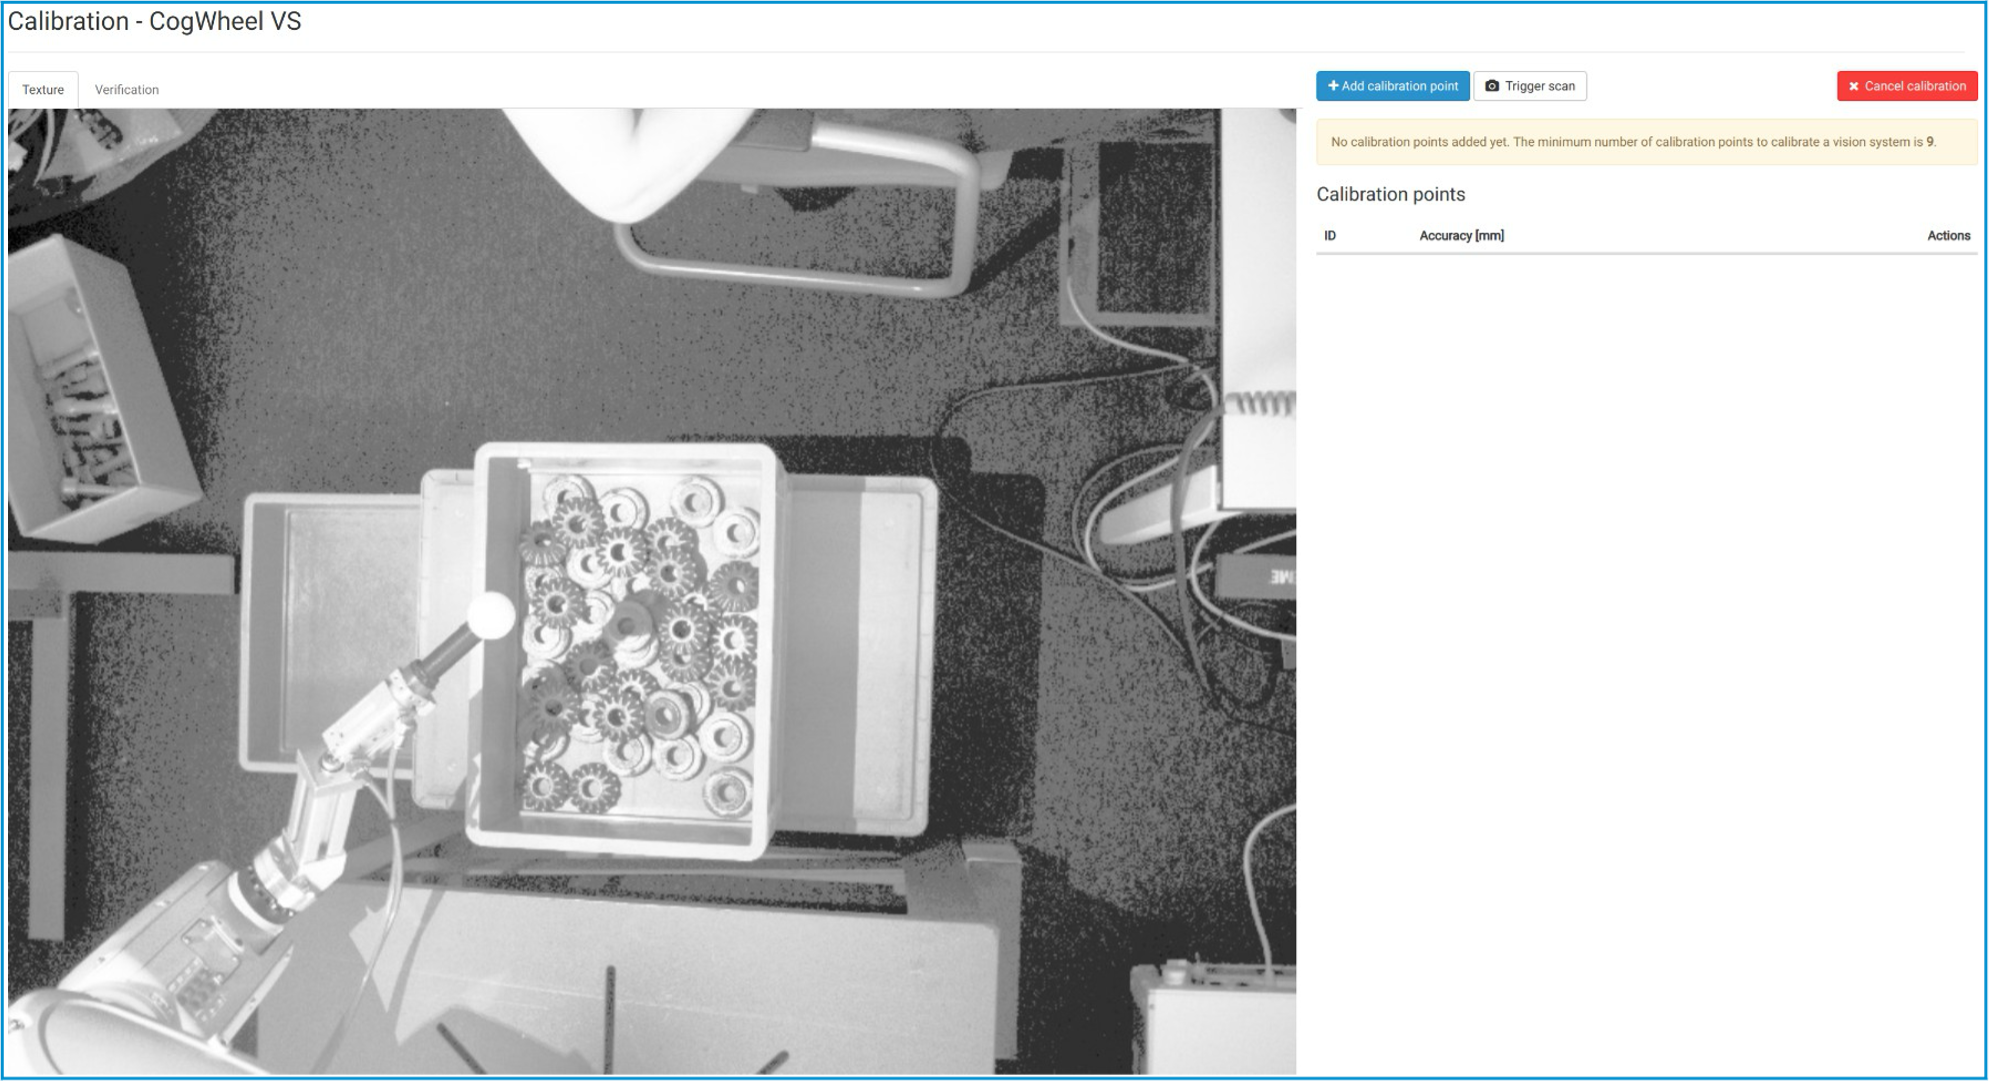
\includegraphics[width=12cm]{Thesis-report/Figures/calibration_procedure.png}
    \caption{Calibration using the calibration ball [2] }
    \label{fig1.Photoneo Cmaera}
\end{figure} 

\item  ● Trigger scan: a button for starting a new scan, typically used to obtain the current point cloud for verification purposes [2]
\item  ● List of calibration points: a list of all successfully added calibration points with individual accuracies and the option to delete a point. The outcome of the calibration process is the calibration matrix. [2]
\item  ● Accuracy of calibration: overall calibration accuracy 
\item ● Finish and save result: button to complete the calibration process and save the calibration matrix result into the vision system [2]\\
\end{enumerate}

The 3D sensor must record the calibration ball in several locations throughout the entire region of interest during the extrinsic calibration process.  In a similar vein, the 3D sensor must record the marker plate from multiple perspectives during the hand-eye calibration.  As a result, move the robot in a variety of positions with as many different joint orientations as you can, and in each position, add a new calibration point.[2]

Either a new calibration point is introduced:
\begin{enumerate}
    \item The Add calibration point button in the calibration web interface can be manually pressed by the operator.[2]
    \item The robot can call the Add calibration point request.[2]
\end{enumerate}

 The scan acquisition is initiated, and the calibration tool (ball/pattern) is detected with the addition of a new calibration point.  A flash message alerting the user to the successful outcome appears if the detection is successful.  A permanent error notice that explains the reason and how to fix the mistake will appear if the calibration point is not inserted [2].

\begin{figure}[h]
    \centering
    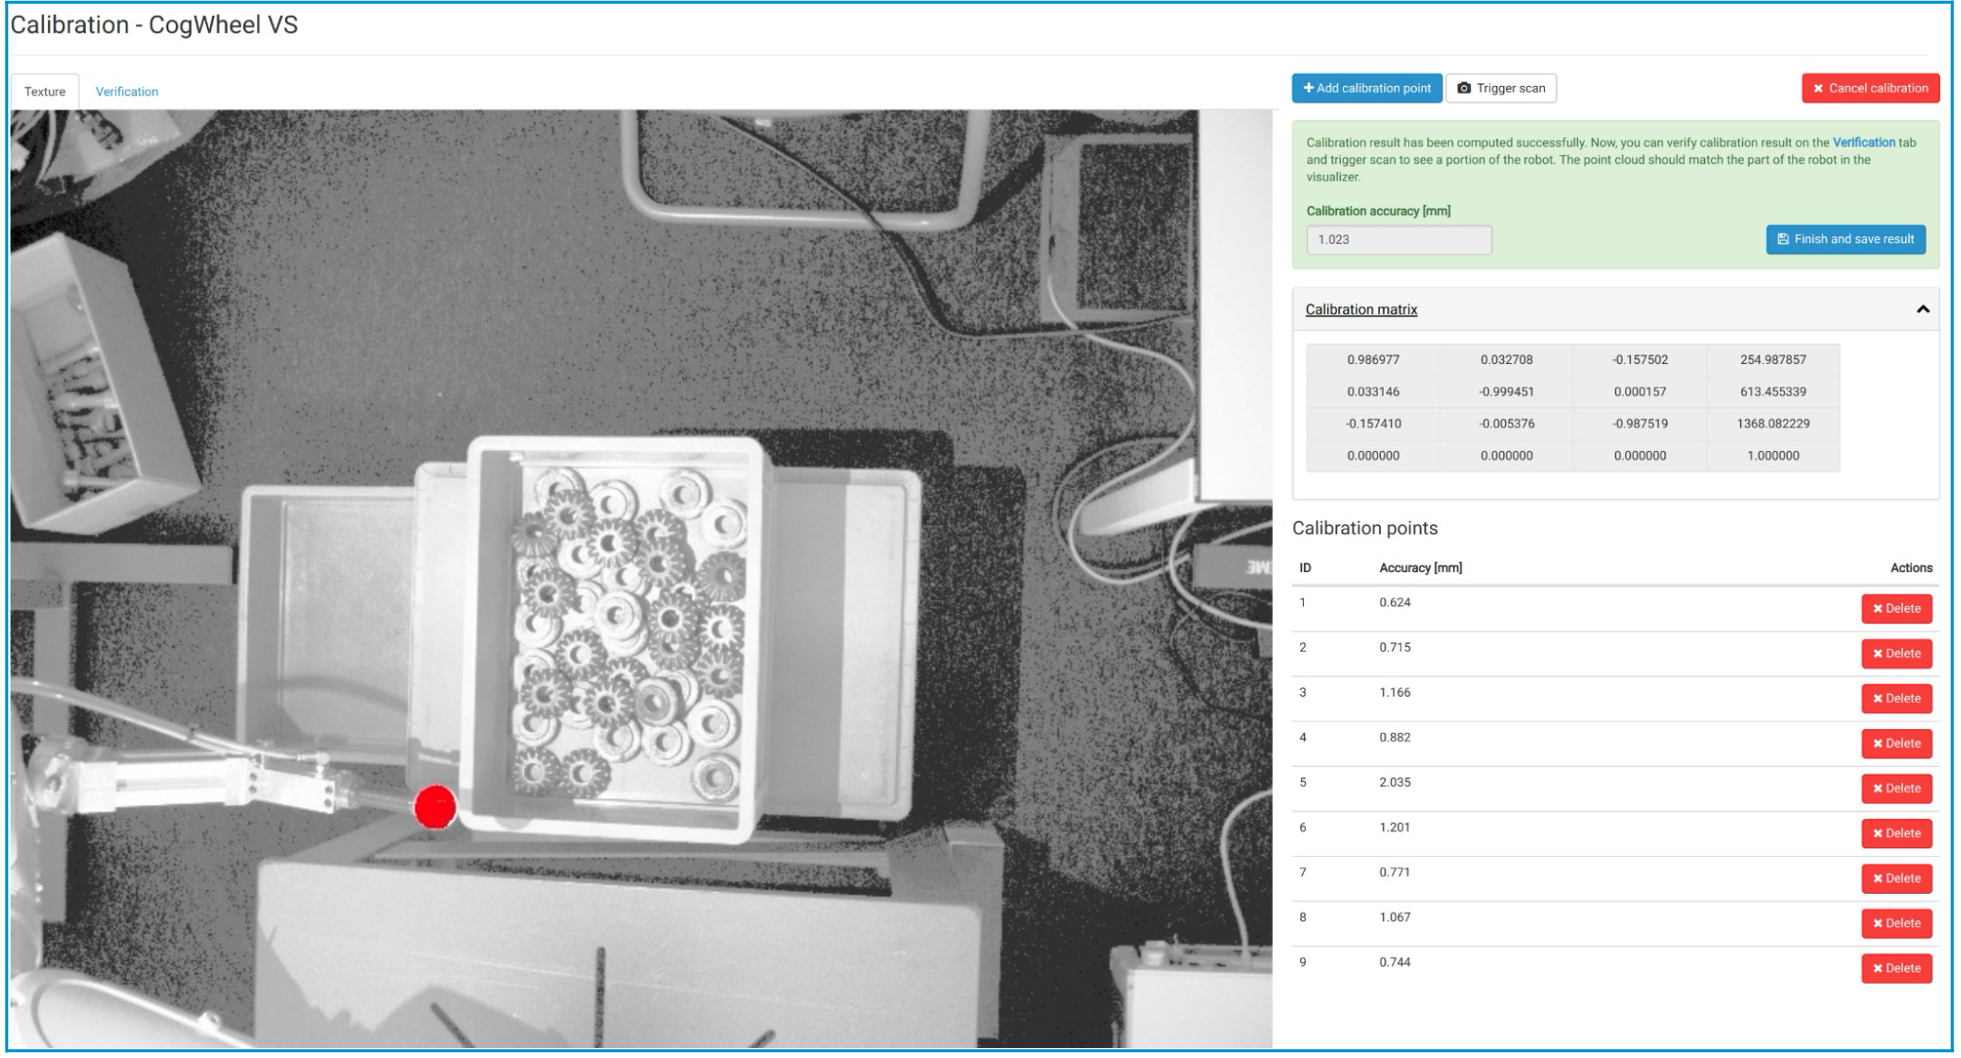
\includegraphics[width=12cm]{Thesis-report/Figures/point.png}
    \caption{Calibration point saved [2] }
    \label{fig1.Photoneo Cmaera}
\end{figure} 

Three calibration sites are needed for both the hand-eye and extrinsic calibration. Once the necessary number of calibration points has been added, the resulting calibration matrix and the calibration accuracy information are only available [2].
 
 Position of 3D sensors and point clouds
 The model of the 3D sensor of the currently calibrated vision system begins to reflect the pose of the real 3D sensor when the 4th point is added during the extrinsic calibration and the Lth point is added during the hand-eye calibration.  The point cloud is shown simultaneously.\\
 Every calibration point that has been successfully inserted has an ID and a unique accuracy score that is measured in millimeters.  The confidence level in correctness increases as the accuracy score decreases.  The Delete option can be used to eliminate a point from the dataset if its accuracy score is excessively high.
 \subsection{Extrinsic Calibration Results:}
\begin{table}[h!]
\centering


\label{tab:transformation_matrix}
\scalebox{1.3}{
\begin{tabular}{|c|c|c|c|}
\hline
-0.327147 & -0.736148 & 0.592503 & -1171.593426 \\
\hline
-0.944628 & 0.271707 & -0.183991 & -234.525444 \\
\hline
-0.025543 & -0.619888 & -0.784275 & 685.496959 \\
\hline
0.000000 & 0.000000 & 0.000000 & 1.000000 \\
\hline
\end{tabular}
}
\caption{Calibration Results}
\end{table}

 The total calibration accuracy score, reported in millimeters, is a measure of calibration quality.  Attempt to score the lowest possible score at all times.  Numerous elements, including the robotic arm size, the quality of the calibration ball, scanning parameters, lighting circumstances, and the 3D sensor, all have an impact on the value.  It is OK to have an accuracy value of a few millimeters. The calibration accuracy value is used to confirm the quality of the calibration.

 Additionally, by assessing the location of the 3D sensor and the point cloud in the picture, the roughly accurate result (without accounting for precision) may be verified.
 The scene's origin is found in the coordinate frame of the robotic controller that was used for the calibration process.  That usually refers to the robot base's origin.  Then, the relative positions of the actual 3D sensor and the robot base in reality should be comparable to or identical to those of the model of the 3D sensor and the scene origin.
 
\newpage
\subsubsection{Calibration of Conveyor Belt}.

The conveyor belt calibration can be done as follows:\\

\begin{figure}[h]
    \centering
    \includegraphics[width=13cm]{Thesis-report/Figures/conveyor_belt with cmaera.jpg} 
    \caption{Coveyor tracking setup}
    \label{fig1.Photoneo Cmaera}
\end{figure}

The above figure consists of the inputs and outputs, where the inputs include:\
\begin{itemize}
\item \textbf{Scan request}\\
The Scan request consists of a  Python code that is used to send a request to the camera, which is then taken by the vision controller or the vision control box that helps trigger the camera.
 \item \textbf{Trigger scan}[21]\\
 The trigger scan can be of the SW or HW method, where the output is hardware or software.

\item \textbf{Trigger }\\
Initially, the scan request is given to the Vision controller, creating a trigger scan that helps the camera trigger.[21] 
The output section includes the following:
\end{itemize}
\begin{itemize}
\item \textbf{Coordinates of localized object}\\
The coordinates of the localized object consist of the object [X, Y, Z, Rx, Ry, Rz, and W], where X, Y and Z include the coordinates of the object and [Rx, Ry, Rz, and W] include the quaternion values (rotation values), which are identified by the vision camera.[21]
\item \textbf{ Scan}\\
Once the trigger commands reach the camera, the scan will start to take place and take the objects as mentioned above.[21]
\item \textbf{Final position} \\ 
The final position is considered the location where the object coordinates, along with the calibration offset and traveled distance.[21]
\end{itemize}


1. \textbf{Calculate the pick pose:} \\\\
2. \textbf{Components of the pick pose calculation:} 
Coordinates from localization in marker space (calculate the transformation matrix from camera space to marker space to calibrate the marker pattern)

Possible triggers for the distance traveled from acquisition to the beginning of picking in conveyor tracking mode include:\\\\
The scan request function pho_wait_for_req_completion() in SW-HW output of the trigger\\\\

\textbf{Calibration Distance:}
The distance between the marker pattern positions for the camera calibration and custom workspace calibration (the linear transformation between the camera and the custom WS origin) is known as the calibration distance.\\

\textbf{Localized posture minus calibration distance plus traveled distance from the scan is the formula.} \\

\begin{figure}[h]
    \centering
    \includegraphics[width=16cm]{Thesis-report/Figures/conveyor_belt.jpg} 
    \caption{Coveyor Belt setup [21]}
    \label{fig1.Photoneo Cmaera}
\end{figure}
In the below figure, we can see the conveyor belt having the calibration board that is used for the calibration, which determines the X, Y, and Z coordinates of the object along with the conveyor belt, where MSD means marker space displacement, TD means travel distance, and TSc means trigger to scan completion in meters where the target position is the T[X, Y, Z, Rx, Ry, Rz], which represents the quaternion value of the object that needs to be converted into Euler values that are used to move the robot to that specified location [21] \\


In the below figure, the number represents the coordinates of the object after the scanning of the object is done after the trigger. Once these quaternion values are attained, these values are then sent to the robotic controller for the robot to move to the required target position.\\\\
\begin{figure}[h]
    \centering
    \includegraphics[width=16cm]{Thesis-report/Figures/coordinates.png} 
    \caption{Coordinates of object}
    \label{fig1.Photoneo Cmaera}
\end{figure}
\newpage
Calibration of the marker pattern from the camera to the conveyor belt, which is the common origin:
\begin{enumerate}
    \item Attach the appropriate calibration pattern to the conveyor belt. [21]
    \item Use PhoXi Control's marker pattern to save calibration. We can use this setting as a custom scanning profile in VS Space by adding a triggering item for the sensor at the marker pattern export photo's origin.[21]
    \item Robot to conveyor belt: The robot moves the conveyor belt from a shared origin, but the marker pattern stays in place according to the conveyor belt. This allows the robot to reach the marker pattern, calibrate the custom coordinate space in the robot track, and save the "calibration" encoder value, which synchronizes the robot and conveyor.[21]\\
\end{enumerate}

\subsection{Conditions for Conveyor Belt:}
While setting up the conveyor belt with a Vision Camera, we need to follow certain conditions:

1. \textbf{Matching the robot speed with the conveyor belt:} For the robot to pick up the object from the conveyor belt, the robot`s end effector should move at the same speed as that of the conveyor belt.\\

\[
V_c = V_r
\]

where \( V_c \) represents the velocity of the conveyor belt and \( V_r \) represents the velocity of the robot.\\

2. \textbf{Target Position Calculation:} The final position of the robot is calculated by:

\[
\text{Target} = TX + AMS \cdot \theta + TD
\]

\text{where } TX \text{ is the initial detected position, } AMS \text{ is the marker space displacement, and } TD \text{ is the tracked distance.}\\

3. \textbf{Marker Space Displacement(AMS):} \\

\[
AMS \cdot \theta = TX - \text{Marker Pattern Origin}
\]

\text{where } TX \text{ is the initial detected position, } AMS \text{ helps in getting the relative position to this reference, and the Marker Pattern Origin is the reference

4. \textbf{Tracked Distance:} 

\[
TD = \Delta TSC + \Delta CTO
\]

Where:

- \( \Delta TSC \) is the \textbf{Target Scan Completion Distance}, which is the distance moved by the conveyor while scanning is completed.
- \( \Delta CTO \) is the \textbf{Conveyor Tracking Offset}, which is the distance moved while waiting for the robot to reach the pick position.

5. \textbf{Target Scan Completion Distance (TSC):} 

\begin{center}
    \[
    TSC = V_c \times t_s
    \]
\end{center}

6. \textbf{Final Adjusted Position:}\\

After considering the conveyor motion and processing delays, the final position will be the place where the robot should pick the object.\\

\[
\text{Target} = TX + (TX - \text{Marker Pattern Origin}) + (V_c \times t_s) + (V_c \times t_r)
\]

\subsection{Manual Calibration}
Initially, before we start the calibration, we need to set the camera to a specific profile setup to Marker Space according to the calibration setup and save the profile as given below: [2]

\begin{figure}[h]
    \centering
    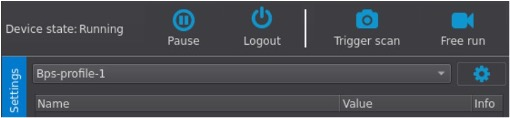
\includegraphics[width=16cm]{Thesis-report/Figures/scanning_profile.jpg} 
    \caption{Scanning Profile [2] }
    \label{fig1.Photoneo Cmaera}
\end{figure}


This method can also be used to get the Conveyor belt calibrated. The steps include :
\begin{enumerate}
    \item \textbf{First step:}  Place the picking / triggering object in the field of view of the camera and trigger the camera, then get the object pose, which includes the [X1, Y1, and Z1] respectively [2]
    \item \textbf{Second step:} Switch on the conveyor belt and get the farthest position where the camera triggers the object, and get the coordinates which include the [X2, Y2, and Z3] respectively.[2]
    \item \textbf{Third step:} While triggering the camera in the first and final position,n we also try to capture the timestamps of the camera, which calculates the time taken by the camera to trigger.[2]
    \item \textbf{Fourth step:} In this step, we need to calculate the change in the position for the X, Y, and Y, respectively, which includes ($\Delta X$, $\Delta Y$, and $\Delta Z$ ). In addition to that, we need to get the change in time also  ($\Delta t$).[2]
    \item \textbf{Fifth step:} In this step, we need to find the custom velocity by dividing the change in the position by the change in time.[2]
    \item \textbf{Sixth step:} Finally, we need to multiply the custom velocity with the time and changes in postion along the X position, which will help in getting change in the position as linear motion and transfered to the robotic controller that helps the robot to pick the itmes from the conveyor belt.[2]
\end{enumerate}

\chapter{\section{\mbox{Inverse Kinematics }}{{\normalfont\fontsize{14}{16}\bfseries}}
We look at the system model, which includes a nonredundant robot manipulator with n degrees of freedom and a conveyor belt system. The following attributes are presumed to be present in the system model: [14]\\
1) The conveyor belt system runs at constant velocity, and the
part is stationary concerning the conveyor belt system.[14]\\
2) The orientation of the robot hand is aligned with the part
initially and kept fixed while the robot tracks the part.[14]\\
3) The robot tracks the part along a straight line path over the
conveyor belt system.[14]

\begin{figure}[h]
    \centering
    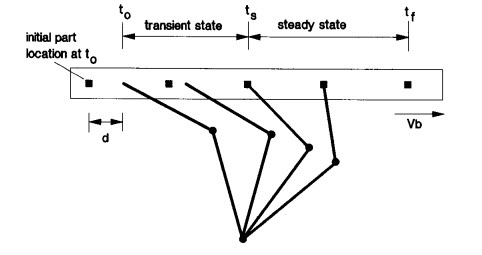
\includegraphics[width=12cm]{Thesis-report/Figures/ik.jpeg}  
    \caption{Kinematics [14]}
    \label{fig1.Photoneo Cmaera}
\end{figure}
The robot motion to be designed must meet certain conditions to maximize the manipulator's usable performance on conveyor tracks. These requirements can be multiplied as follows to create a single differential equation.[14]
\newpage
1) \textbf{Steady-state error:}  The task's accuracy may be reduced due to location and velocity errors in the steady state. Therefore, the steady-state error in the conveyor tracking trajectory must be as low as feasible.[14]\\
2)  \textbf{Constraints on torque and smoothness:}The trajectory must be created so that all joint torques stay within their ranges at all times. The torque limitations are as follows: i = 1,..., 3 n; ut.rnm(t) 5 uc(t) 5 ~c,max(t).[14]\\
3) \textbf{Settling time:}  As the robot rapidly reaches a steady state, the amount of time required for the task is decreased. The settling time should be kept to a minimum while taking into account the robot's torque and smoothness limitations, the conveyor belt's speed, and the initial positions of the robot and the part.[14]\\
The joint variables in the forward kinematics issue establish the end-effector's position and orientation in Cartesian space, also known as the workspace. For rotational joints, the joint variables are the angles between the links; for prismatic joints, they are the link extension. On the other hand, the inverse kinematics challenge is determining the values of the joint variables that enable the manipulator to arrive at the specified location given a desired end-effector position and orientation.
The figure below illustrates the connection between joint space and Cartesian space, as well as the relationship between forward and inverse kinematics.[10]\\

\begin{figure}[h]
    \centering
    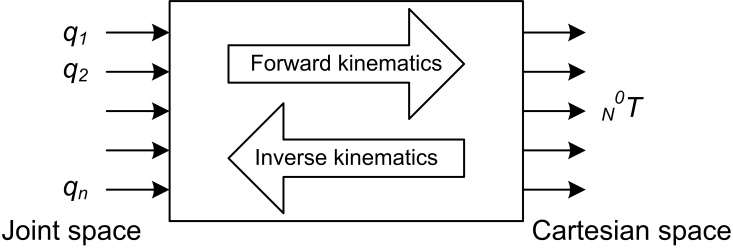
\includegraphics[width=12cm]{Thesis-report/Figures/fk.png}  
    \caption{Forward and Inverse Kinematics [10]}
    \label{fig1.Photoneo Cmaera}
\end{figure}
Finding the joint variables that allow a robot to be manipulated into the required position requires an understanding of its inverse kinematics. This is used to control the robot's position, motion, and other features. This study presents a detailed explanation and comparison of two popular approaches for manipulating robots: Jacobian inverse techniques and inverse kinematics.[10]
Sixteen alternatives are available for a general six DOF robot, as shown below, and it lists the number of analytical solutions for robots with varying degrees of freedom. Therefore, an accurate set of solutions among several inverse kinematic solutions is needed for the continuous motion of a robot.[10]

\\ The benefit of analytical expression is that it provides formulas for the connection between link parameters and joint angles. The robotics controller can directly incorporate these relationships.[10]\\

\begin{table}[h]
    \centering
    \begin{tabular}{cc}
        \toprule
        \textbf{DOF} & \textbf{Number of Solutions} \\
        \midrule
        6 (6R, 5RP) & 8 \\
        6R (intersecting wrist)
Greater than 6 & 16\\
        (Redundant manipulator) & ∞\\
        \bottomrule
    \end{tabular}
    \caption{DOF vs. Number of Solutions [19]}
    \label{tab:dof_solutions}
\end{table}
\newpage
\subsection{Working Flowchart:}
\begin{enumerate}
    \item Start
    \item Initially, check if the operation type is OBJECT POSE
    \item If no, then assert an issue showing that there is an unexpected issue.
    \item If yes: Receive object pose data
    \item Then unpack the object pose and set them as ([X,Y,Z.ex.ey.ez])
    \item Convert the first three elements to meters ([X.Y, Z])
    \item Set the velocity and timeout for picking
    \item Record the start time
    \item Calculate the current time and update the position X with the equation ([X=X0 + velocity *t])
    \item Create the target position with the quaternion values received from the camera
    \item Check the condition where the object needs to be picked, if the distance is less than 700, then do the motion of move linear ()
    \item If not success:  break the loop and print the target is too far
    \item Get the current joint angles and TCP Pose, and calculate the distance to the object.
    \item If the distance to the object is less than 5, then send the signal to the gripper and pick the object.
    \item If the timeout to pick is greater as compared to the given input, then break the loop.
\end{enumerate}
\newpage
The following figure shows the flowchart for the Dynamic Picking:\\
\begin{figure}[h]
    \centering
    \includegraphics[width=8.3cm]{Thesis-report/Figures/Flowchart.jpg}  
    \caption{Flow Chart}
    \label{fig1.Photoneo Cmaera}
\end{figure}
\newpage
\subsection{Jacobian inverse method}:\\
The time derivative of the kinematic equations that connect the end-effector's velocity to the joint rates is known as the Jacobian in robotics. The following is the phrase for the Jacobian.[19]
\[
\omega_e = J_{\omega} \theta, \quad v_e = J_v \theta [19]
\]
where the 3x6 matrices J ω and J v relate the joint velocities or rates θ to the end-effector angular velocity ω e and velocity v e, respectively. Also, J ω and J v are where J  J (JJ) is the function of θ and the pseudo-inverse of the J matrix. It is possible to rewrite as:[19]\\
\[
\Delta x_e = J \Delta \theta [19]
\]
where,
\[
\begin{bmatrix} 
\Delta \phi \\ \Delta \theta \\ \Delta \psi \\ \Delta x \\ \Delta y \\ \Delta z  [19]
\end{bmatrix}^T
=
J
\begin{bmatrix} 
\Delta \theta_1 \\ \Delta \theta_2 \\ \Delta \theta [19]
\end{bmatrix}

The change in the end-effector's pose that corresponds to the change in joint angles θ is denoted by the word x. The recursive relationship between the angular velocity and linear velocities for a 6R manipulator yields the Jacobian J, which is a 6×6 matrix for a 6-DOF robot. It is provided as [19]\\


\[
J =
\begin{bmatrix}
0 & e_1 x a_1 & e_1 \\
e_6 & e_6 x a_6 & e_6 \\
\end{bmatrix}
\]

where a1 is the joint axis direction of joint 1 and e is the vector. Likewise, direction and is the joint axis a2, e is the EE's location from joint 2, and so forth. The differential rotation and translation vectors that correspond to the differential change in the joint rates make up each column of the Jacobian. The Jacobian inverse provides the joint variation for the desired increment at the kth point pose as follows:[19]\\
\[
\Delta \theta_k = J_k^{-1} \Delta x_e [19]
\]
where Xe represents the required increase in the EE's posture. The effective method for determining the increment was provided. Joint angles needed to get to the kth point are comparable to the joint angle's first-order Taylor series expansion, which is calculated as:[19] \\

\[
\theta_k = \theta_{k-1} + J_k \Delta x_e [19]
\]
\[

In general, \theta_k = \theta_{k-1} + J^{\dagger} \Delta x + (I - J^{\dagger} J) \Delta \phi [19]
\]

where \[
J = J (JJ) [19]
\]
 is the null space of J with phi as the objective function, and J = J (JJ) -1 is the pseudo-inverse of the matrix J. x J.[19]
Since the Jacobian matrix is square and invertible, it is utilized in this case for the manipulator with DOF = 6. [19]\
\subsection{Robot Coordinate System} 

We must first gain a fundamental understanding of the Robot Coordinate System before delving deeper into the tracking system's operation. Generally speaking, robotic systems are Cartesian coordinate systems with three axes: the X, Y, and Z axes. Additionally, there is the Rotation Coordinate System, which describes the robot's degree of rotational motion and joint function. However, as this format is more widely used in the business and simpler to use and comprehend, we shall solely investigate the Cartesian coordinate system. For getting the robot coordinates, we should be  aware of the following terms used in the system:\\\\
 \textbf{System of World Coordinates (WCS):} \\
A coordinate system is often specified by the user or developer, but it can exist anywhere in the world. As long as WCS makes it simpler to explain the locations of other things or items in that specific area, you can put it anywhere in your room or factory. Origin placement is typically done at the edge of a group or a room's corner.\\\\
 \textbf{Machine Coordinate System (MCS):} \\
Robot Base Frame Coordinate System is another name for Machine Coordinate System (MCS). All other coordinate systems will be compared to this most significant coordinate system. Where developers and programmers would implement their code based on this coordinate system is equally crucial. MCS is typically positioned near the robot's base for the point of origin, though it's important to remember that different robot types have different bases.\\\\
\newpage
 \textbf{Coordinate System for Parts and Workpieces (PCS):} \\
This refers to the workpiece or tracked objects that travel along the conveyor belt. In certain applications, part orientation plays a crucial role in assembly procedures. In our application, we just want to choose or select the objects, independent of their orientation; thus, this isn't accurate.\\

 \textbf{Tool Coordinate System (TCS):} \\
 This refers to the location of the robot's end-tool tip. As you can see, a robotic hand typically has a mechanism attached to the end, either a vacuum or a gripper. When referring to the robot base frame, this typically requires a little amount of offset and aids the robot in completing its responsibilities.\\\\
 \textbf{ Coordinate Transformation Matrix:}  \\
 In essence, the coordinate transformation matrix is a matrix that depicts how a coordinate system's orientation changes from one frame to another. It describes rotation transformation and translation transformation, and is composed of a 3x3 rotation matrix and a 3x1 displacement vector. In the case of three dimensions, the matrix is 4x4. A more common and widely used name for this matrix is the homogeneous transformation matrix. Remember that this matrix can be applied to any coordinate transformation situation, including regular coordinate transformation operations and forward kinematics derivations.\\\\

\begin{figure}[h]
    \centering
    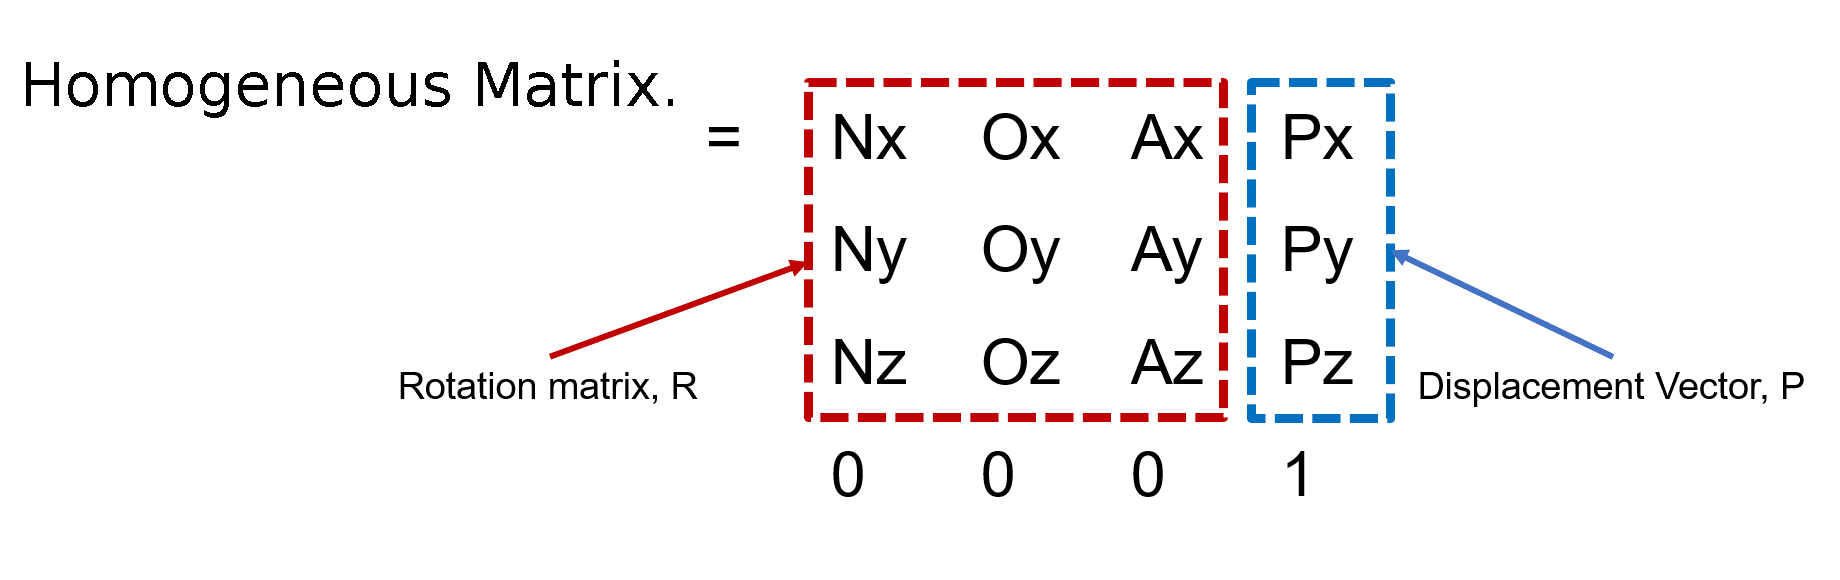
\includegraphics[width=15cm]{Thesis-report/Figures/transform.png} 
    \caption{Homogenous transform}
    \label{fig1.Photoneo Cmaera}
\end{figure}
\textbf{ Operations Needed to Develop the Tracking System:} \\
The tracking system's pillars are composed of three primary components. Only a scenario including a camera, a belt conveyor, and a robot will be covered in this post. It is certainly possible to expand the tracking system by including additional robots and cameras. Although more intricate procedures will be required to make up for the additional components, the fundamentals will remain the same.\\

1. \textbf{ Conveyor Belt to Camera Conversion (B1):} \\
The orientation of the conveyor belt coordinates and the camera origin coordinates deviate from one another. The origin of a camera is the upper left corner of its field of vision (FOV), where the values of its pixels start at (0, 0). This origin is set in stone and cannot be altered. For the conveyor belt, we can freely provide the origin's location, but the standard procedure is to first specify the picking window's dimensions (it's square), taking into account the robot's picking range limit, and then place the origin at the center of the window's bottom.\\

\begin{figure}[h]
    \centering
    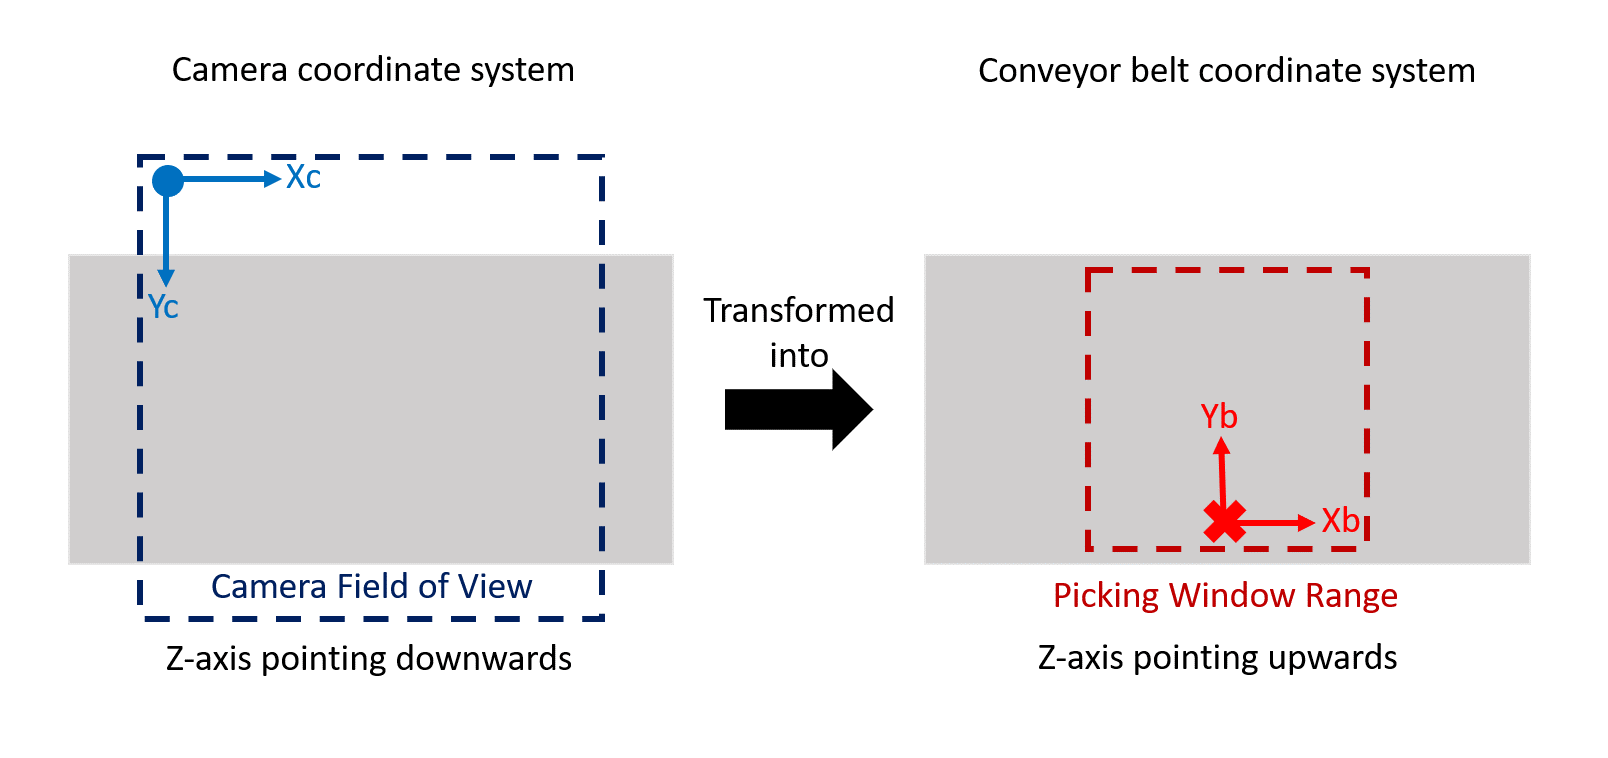
\includegraphics[width=15cm]{Thesis-report/Figures/camera to conveyor.png}
    \caption{Conveyor to camera conversion}
    \label{fig1.Photoneo Cmaera}
\end{figure}
As can be seen from the above image, to match the conveyor belt origin, we must perform a translation transformation in both the X and Y axes. We must do a rotation transformation for the Z-axis since the belt origin faces the other direction from the camera origin. In summary, this section contains two transformations: Rotation transformation, Rot(x, 180°); AND Translation in the X-axis and Y-axis, Trans(ΔX, ΔY, 0). Observe that both the Y and Z axes changed their facing directions when we rotated the X axis. For this section, some offset will be required.\\

2. \textbf{ Conveyor belt (B1) to conveyor belt (B2) transformation:} \\
For this part, it is quite simple. This transformation is about the movement of the conveyor belt from the Camera’s Field of View to the Robot’s Workspace/Pick range. The only value that changes in this transformation is the X-axis value. As mentioned in the introduction, we also include the encoder’s reading to help us track how much distance the conveyor belt covered.\\

\begin{figure}[h]
    \centering
    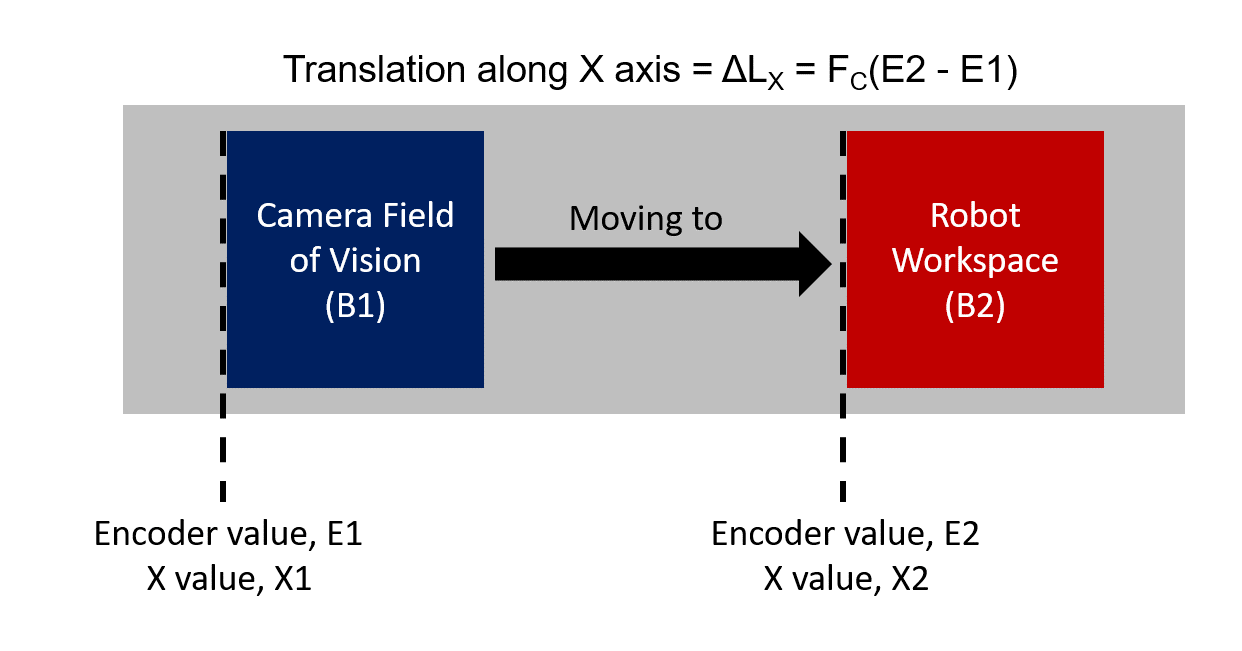
\includegraphics[width=10cm]{Thesis-report/Figures/cam to conv.png}
    \caption{Conveyor belt b1 to b2 conversion}
    \label{fig1.Photoneo Cmaera}
\end{figure}
\subsubsection{Encoder offset}
Types and Technologies of Encoders
Although encoders come in a wide variety of forms, they essentially fall into two primary sensing categories. These include:

\begin{enumerate}
    \item  Linear
    \item Rotating
    
\end{enumerate}

There are various encoder measuring types within those categories, including:
\begin{enumerate}
    \item Complete
    \item Gradual
\end{enumerate}
Additionally, there are several electromechanical technologies, including:
\begin{enumerate}
    \item Magnetism
    \item Optical
    \item Inductive
    \item Capacitive
    \item Laser \\\
\end{enumerate}
    
\chapter{\section{\mbox{Working Principle }}{{\normalfont\fontsize{14}{16}\bfseries}}
\subsubsection{Steps for Conveyor Tracking Visual System:}\\
Two steps are necessary for conveyor visual tracking: [12]\\
\begin{itemize}
\item Item detection\\
\item Object tracking.\\
\end{itemize}\\
There are several ways to identify items. Some potential limitations are, however, information-based recognition, self-organizing maps, template matching, and the temporal difference between two consecutive image samples. Due to their slowness, self-organizing maps cannot function in real-time. Template matching requires prior knowledge of object information to match objects. Unfortunately, because of the necessary computational load, this method cannot be used in real time. The color information solution overcomes the first two limitations; however, it is not compatible with binary images. The object recognition method that leverages the difference between two photographs can be useful when the environment does not change quickly over time.[12]
\subsubsection{Photoneo Camera}
The main Vision camera we have used to track the moving object's motion through the conveyor belt is a Photoneocamera (MotionCam 3D M+), which has advanced settings that can capture and detect the object's position.\\\\ The photoneo camera mainly consists of 3D sensing technology, which contains parallel structured light that helps provide the light source to detect the objects. Using this camera, the camera can capture accurate point clouds and a standard intensity image of the object.[2] \

Three parts comprise the 3D camera: a camera unit with our proprietary Mosaic Shutter CMOS image sensor, a laser projection unit, and a processor unit with a GPU that acts as the brain behind intelligent applications. A sequential structured light, which is utilized in numerous meteorological applications, is the primary technological driver in the first group. One well-suited representative of this category is the 3D scanner range from Photoneo. This technique is not appropriate for dynamic scenes because it uses sequential (multi-frame) capturing. This section is the source of the parallel structured light.[2] \

\subsubsection{Robot Interface:}\\
There are two subsections in this section:
\begin{enumerate}
    \item  ● Robot interface: utilized to configure the vision controller's Ethernet port on the network.[2]
    \item  ● Robot controller: utilized to determine the robot controller's IP address.[2]
\end{enumerate}
\begin{figure}[h]
    \centering
    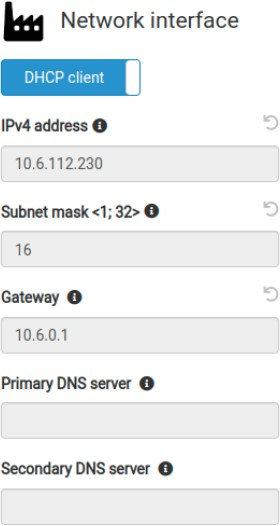
\includegraphics[width=5cm]{Thesis-report/Figures/network_interface.jpeg}
    \caption{Robot Network Interface[2]}
    \label{fig1.Photoneo Cmaera}
\end{figure}
 The Action Request Communication Channel is used to facilitate communication between the vision controller and the robotic controller, as explained in the Robot Communication.  The robotic controller connects to the TCP server created by the vision controller and transmits requests to it.[2]
 It is advised to keep the Action Request Server port section empty and use the default port for this TCP server.  It is necessary to use the same port on the robot side when a custom port is defined.[2]

\subsubsection{Vision controller Interface:}\\
Gigabit Ethernet cables (Cat5e or higher category) are needed to connect the 3D sensor.  A gigabit switch can be used to connect several 3D sensors.  In all situations, the switch or 3D sensor's Ethernet connection is attached to the scanner's network port.[2]
\begin{figure}[h]
    \centering
    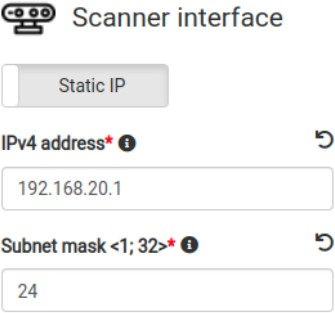
\includegraphics[width=5cm]{Thesis-report/Figures/scanner_interface.jpeg}
    \caption{Robot Network Interface [2]}
    \label{fig1.Photoneo Cmaera}
\end{figure}
\newpage
 Setting up localization settings, calibrating the robot camera, and seeing 3D scans all require a well-configured connection to the 3D Sensor. [2]\\

 To set up the network interface that the vision controller uses to connect to the Photoneo 3D Sensor, go to the Network page and select the Scanner interface section.[2]\\

 Both a fixed IPv6 link-local address and a programmable IPv4 address are features of Photoneo 3D Sensors.IPv6 connections are better than IPv4 ones.  Nevertheless, the IPv4 address is used if the IPv6 connection is banned or fails.  Consequently, having a legitimate IPv4 network configuration is advised.[2]\\

 The interface can be set up to operate a DHCP server or to utilize any random static IP address.  Use the appropriate IP address settings on the sensor side through the PhoXi Control program in both situations.[2]\\

\subsubsection{Communication of Robot With Vision Camera}\\
The robot interface on the vision controller and the robot module operating on the robot controller enable communication between the vision controller and the robot controller.[2]\\

\begin{figure}[h]
    \centering
    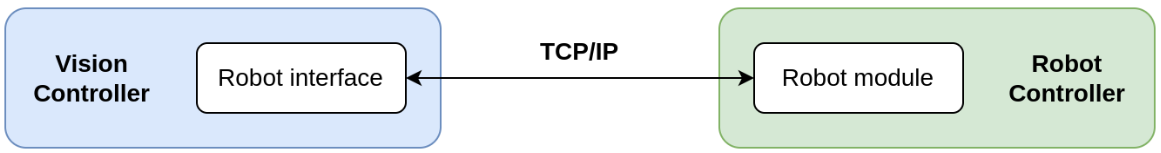
\includegraphics[width=14cm]{Thesis-report/Figures/communication.png}
    \caption{Communication with camera [2]}
    \label{fig1.Photoneo Cmaera}
\end{figure}

The Vision Controller's scanner port is directly attached to a single Photoneo 3D sensor. 
● The vision controller's network port is directly connected to a desktop PC for remote control.
● The robot controller is directly attached to the vision controller's robot port.[2]

\begin{figure}[h]
    \centering
    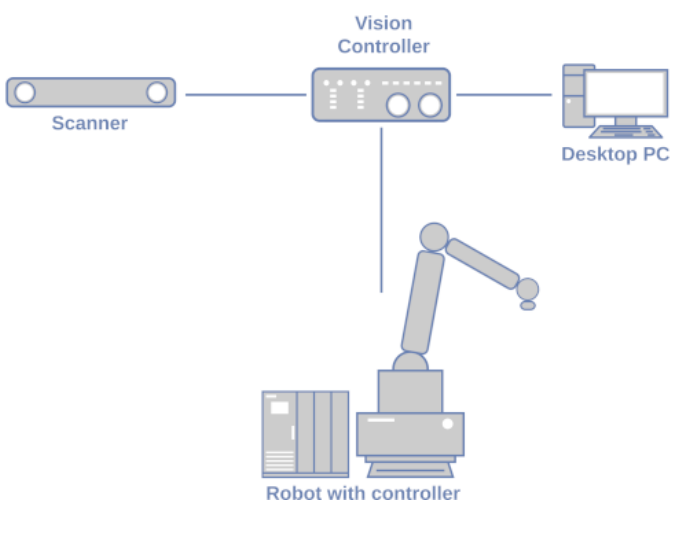
\includegraphics[width=10cm]{Thesis-report/Figures/connection.png}
    \caption{Whole camera with Robotic controller setup [2]}
    \label{fig1.Photoneo Cmaera}
\end{figure}

\newpage
 \subsubsection{Protocol TCP/IP}\\
The robot controller and the vision controller communicate via the TCP/IP protocol. Network connectivity is an optional feature that some robot controllers do not come with by default. All prerequisites for the full installation of the robot module are listed in the robot integration guides' Prerequisites section.[2]

\subsubsection{Channel of communication}\\
The Robot module functions as a TCP client, while the vision controller establishes a TCP server. The client is called the Action Request Client, while the server is called the Action Request Server. The Action Request Client communicates with the Action Request Server over this channel. After receiving the action request, the vision controller carries it out and replies to the robotic controller.[2]\\\\


\begin{figure}[h]
    \centering
    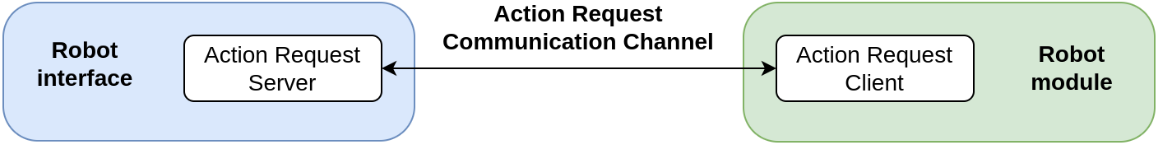
\includegraphics[width=14cm]{Thesis-report/Figures/channel.png}
    \caption{Channel Communication[2]}
    \label{fig1.Photoneo Camera}
\end{figure}
\newpage
The robot connection status is currently indicated by the following indicator:

 Action Request Client: the state of the Action Request Communication Channel connection between the Action Request Server and the Action Request Client.  It may exist in one of two states:[2]
 \begin{enumerate}
     \item  \textbf{CONNECTED:} The Action Request Client can send requests since it is connected to the Action Request Server.[2]\\ 
      \item   \textbf{DISCONNECTED:}  The Action Request Server is awaiting a fresh connection as the Action Request Client is not connected to it.[2]

 \end{enumerate}

 Every vision system has a status indication that shows the current status of the connection to the related Photoneo 3D Sensor.

 \\ Each indicator bears the identification number of the vision system to which it belongs.
  \begin{enumerate}
  \item  \textbf{CONNECTED:} The vision system 1's 3D sensor is connected.[2]
  \item   \textbf{DISCONNECTED:}  There is no connection to the 3D sensor linked to vision system 2.[2]
 \end{enumerate}

\subsubsection{Network (EC, HC) }\\
The robot interface (and robot controller IP) and the Vision controller's 3D sensor interface must be properly configured for the Vision controller to communicate with both the robot and the 3D sensor. This is not required for marker space calibration.[2]
\subsubsection{Vision }\\
It is necessary to thoroughly configure the visual system that will be calibrated. Make sure the following vision system parameters are set up correctly before beginning the calibration:
● Scanner ID: This vision system uses a 3D sensor. The linked 3D sensors will appear in the drop-down list of available 3D sensors if the scanner interface is set up properly.
The calibration space and scanner position specify the 3D sensor's mount point and, consequently, the calibration type. The scanner model is automatically calculated based on the selected 3D sensor.[2]

\subsubsection{6-Axis Cobot-Delta}
The cobot that we have used for the conveyor tracking system is a 6-axis cobot called a Delta robot. The robot mainly moves towards its target position by getting the values from the camera in the form of quaternion values.[2]\
\begin{figure}[h]
    \centering
    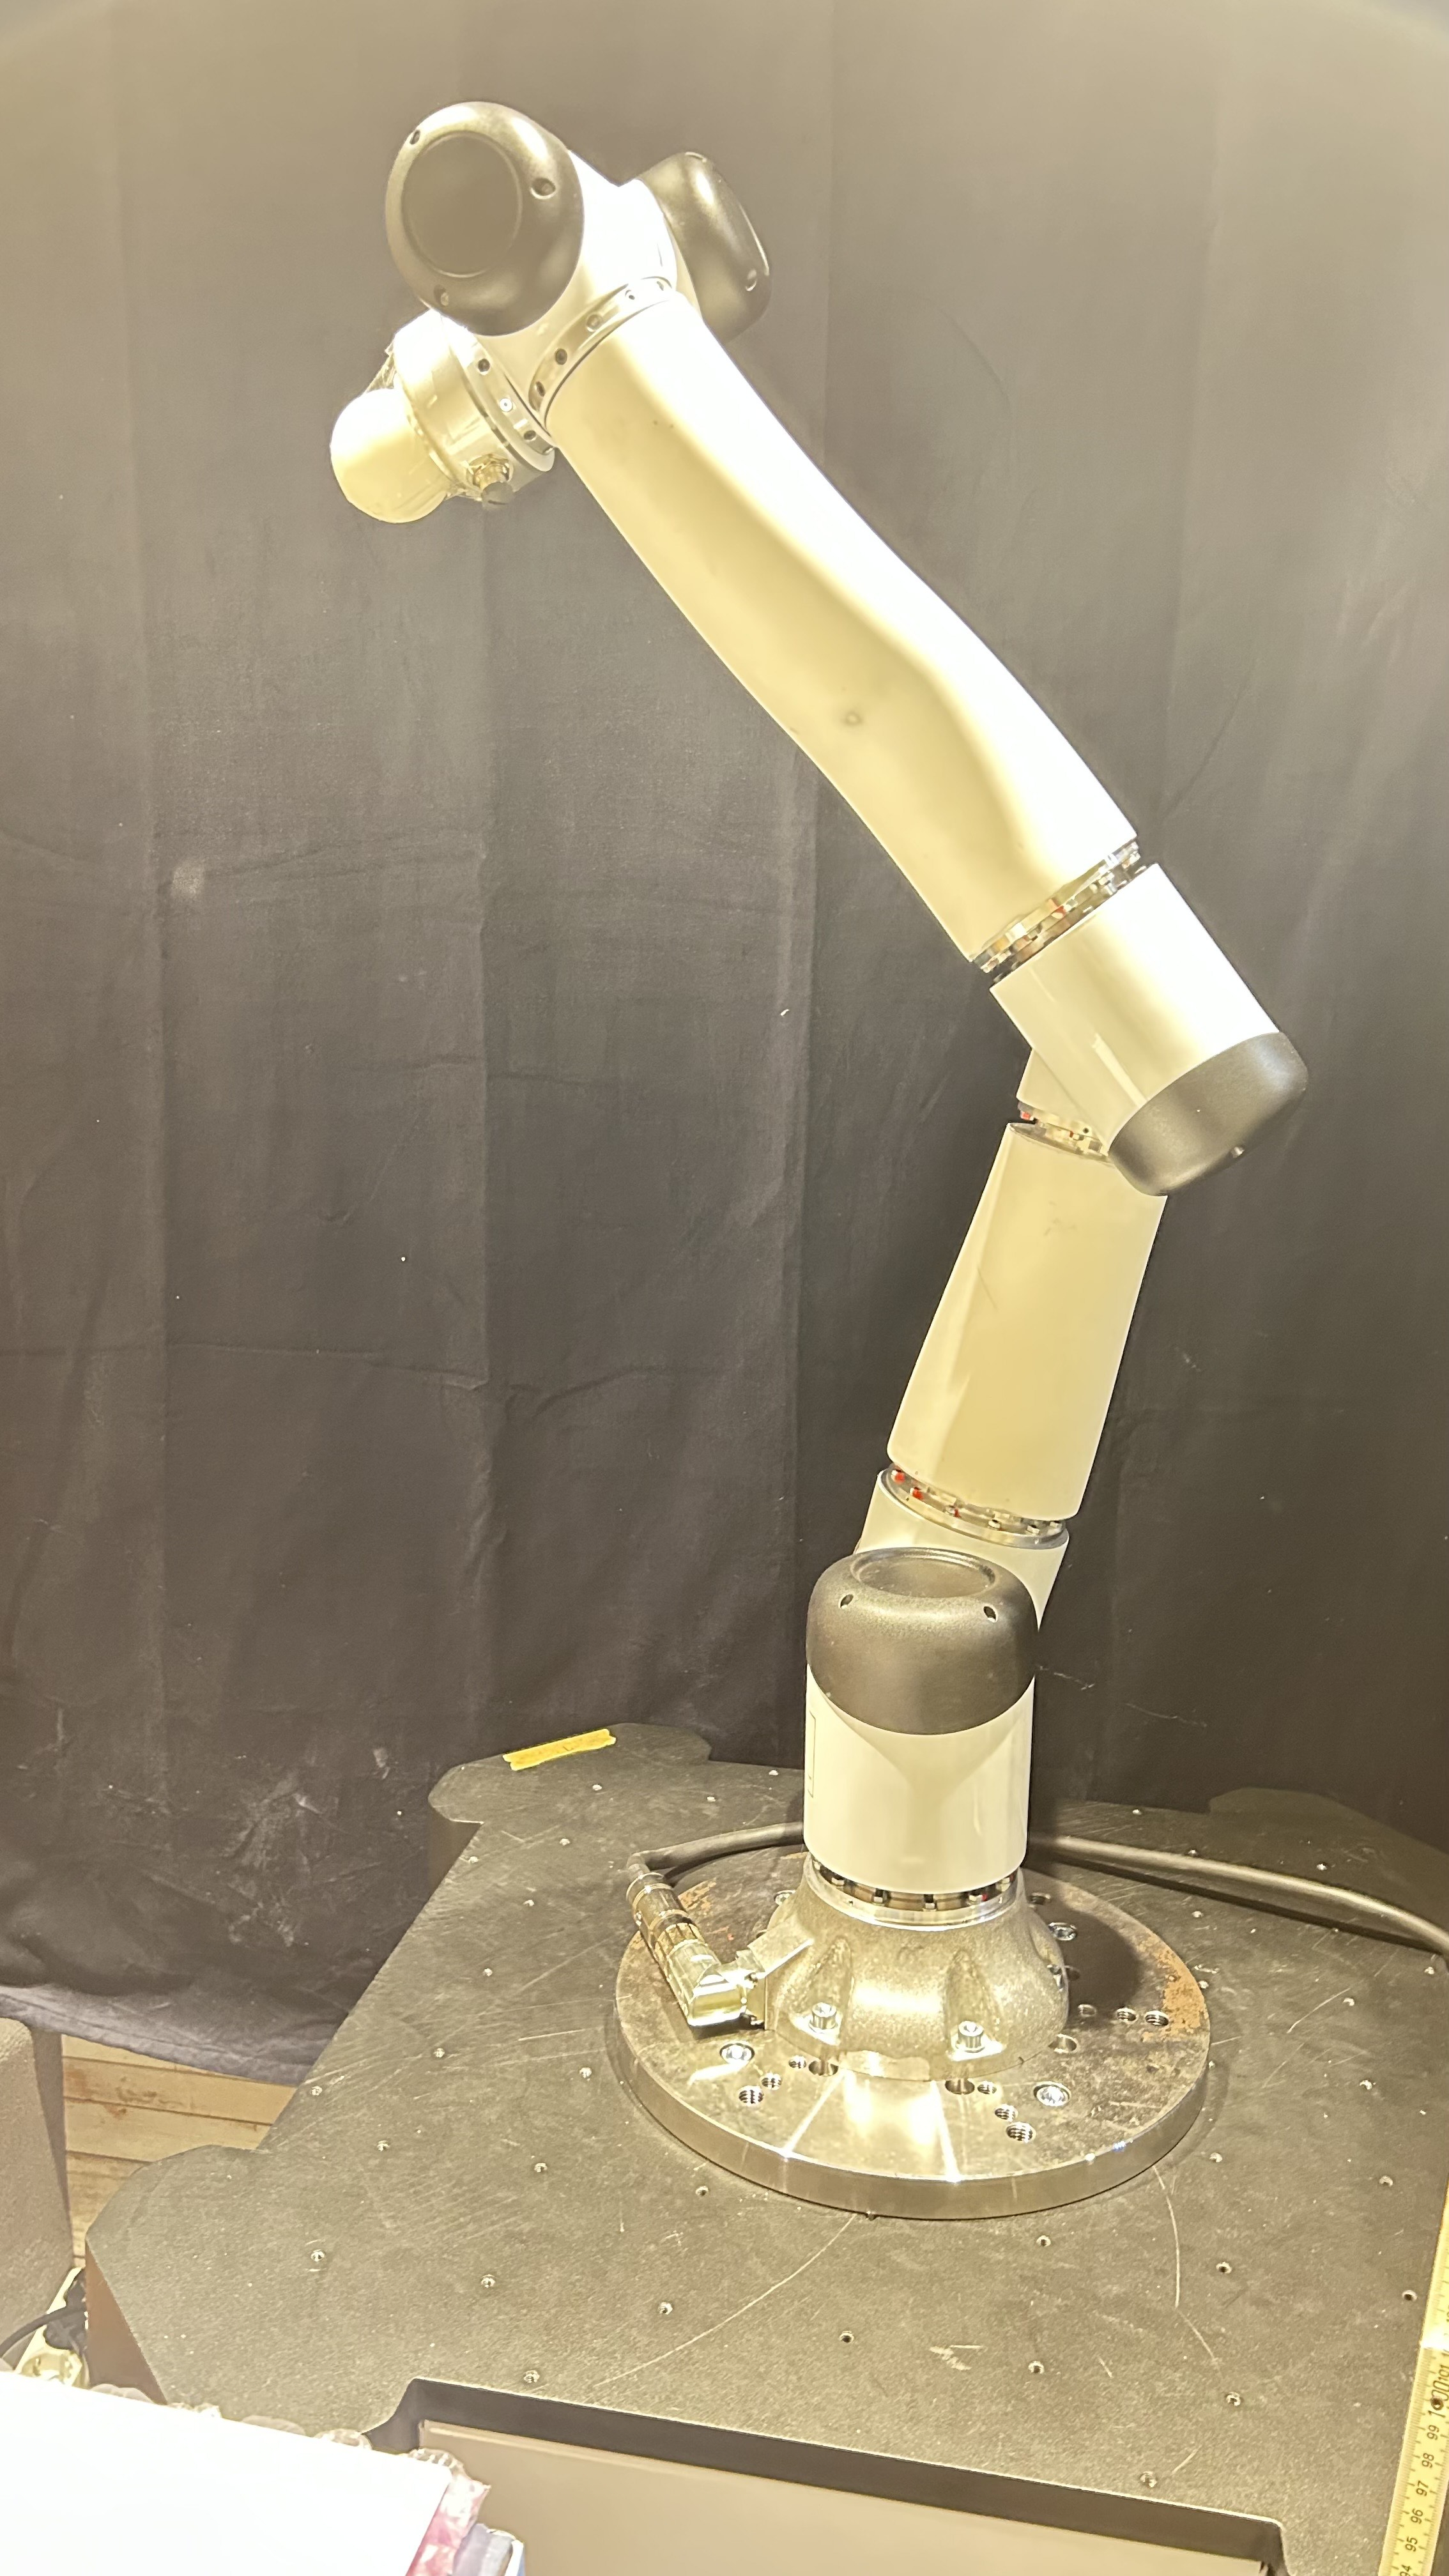
\includegraphics[width=4.5cm]{Thesis-report/Figures/robot.jpeg}
    \caption{Delta Robot}
    \label{fig1.Photoneo Cmaera}
\end{figure}

\subsubsection{RobotiQ 140 Gripper:}
\begin{figure}[h]
    \centering
    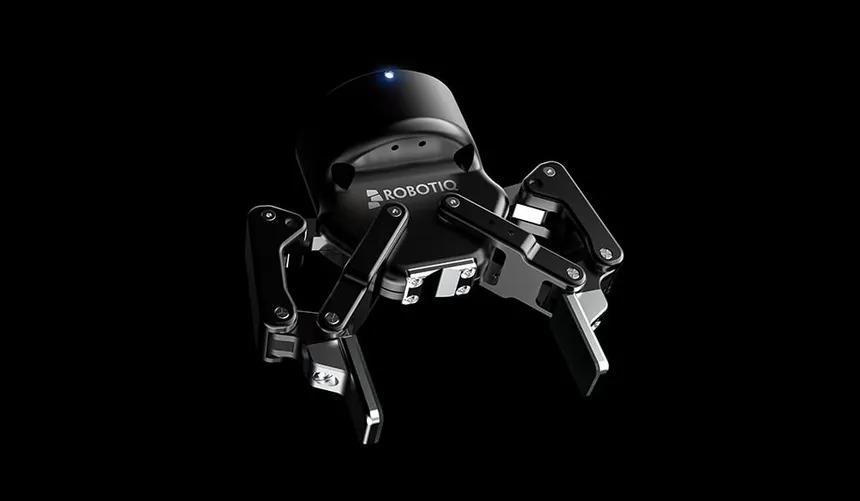
\includegraphics[width=8cm]{Thesis-report/Figures/cobot_gripper_2F_85-ezgif.com-webp-to-jpg-converter.jpg}
    \caption{RobotiQ 140 Gripper}
    \label{fig1.Photoneo Cmaera}
\end{figure}
The RobotiQ 140 gripper is a two-finger gripper that mainly works under the principle of Modbus Communication. This gripper's 85 mm stroke, 230 N maximum gripping force, and 5 kg maximum payload make it the perfect choice for anyone looking for a flexible, all-purpose end-of-arm tool. This gripper is perfect for low-volume, high-changeover settings since it can efficiently grasp a broad range of workpiece sizes and forms.


\newpage
\section{Robotic Movement:}
The Robotic movement can be performed with 3 methods called Servo X, ServoJ,and Movelinear.\
\begin{itemize}
    \item ServoX
    \item Servo J
    \item Movelinear
\end{itemize}\\
1. \textbf{ServoX:} In the Servo X motion, we move the robot in Cartesian motion, where the coordinates that we get from the camera are in quaternion poses [X, Y, Z, Qx, Qy, Qz, W]. These are already in the Cartesian poses, which can be directly passed to the robotic controller, giving these values as the target position, and moving the robot to the desired location. During servoX, the coordinates that came from the camera were not in the correct order as that of the robotic movement, so initially the target position had to be changed as in this form [X, Y, Z, W, Qx, Qy, Qz]\\\\
2. \textbf{ServoJ:} In the servo J, the move of the robot is with the joint movements, rather than the Cartesian. The object coordinates that we get from the camera are in Cartesian form; they need to be converted into joint form and given as the target position. When giving the target position, the final orientation values of the coordinates will not be the same as those of the TCP coordinates of the robot. To set this, we have to implement the method of inverse kinematics.\\\\
3. \textbf{Movelinear:}
The Movelinear is the method in which the target position for the robot to pick up the object is directly given as the quaternion values provided by the camera, by scanning the objects. Here we define the maximum velocity, acceleration. The movement of the robot happens in a servo interface where the quaternion values are sent to the robot as the target position, which helps the robot to the required position.

\subsection{Static Picking:}\\
Static pick-up is the process of picking items from the conveyor belt when it is not moving. Initially, we keep the object on the conveyor belt and then trigger the camera which helps in getting the object coordinates to the robotic controller. When the robot receives the data, the robot moves to the target position to pick the required target.
\begin{figure}[h]
    \centering
    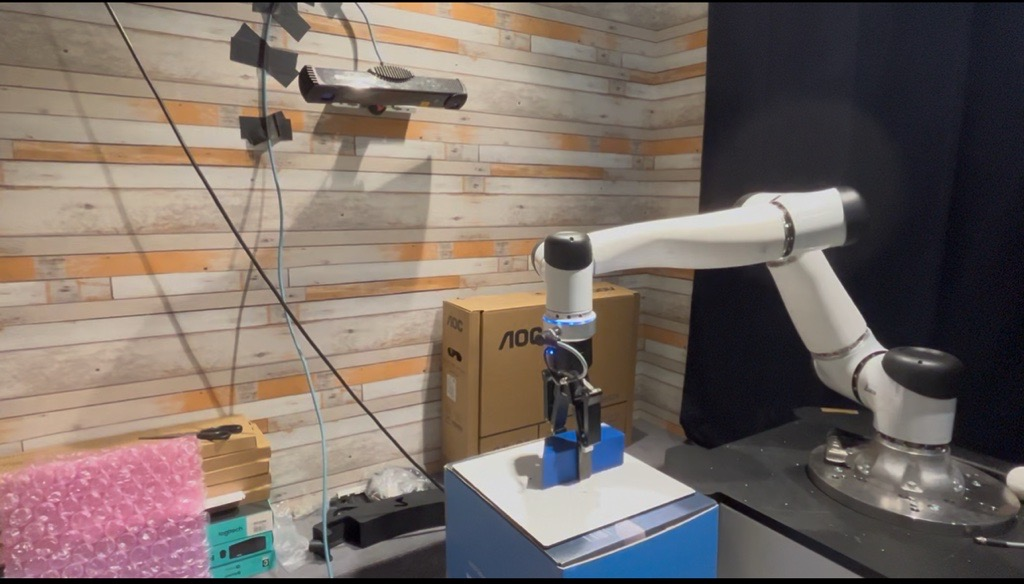
\includegraphics[width=10cm]{Thesis-report/Figures/static.jpeg}
    \caption{Static Picking}
    \label{fig1.Photoneo Cmaera}
\end{figure}


\subsection{Dynamic Picking:}\\
The Dynamic Pick involves the process of picking the items from the moving conveyor belt. Here, the object is passed through the moving conveyor belt, where the camera gets object poses that are passed to the robotic controller, which helps the robot move to the required position.\\
\begin{figure}[h]
    \centering
    \begin{minipage}{0.45\textwidth}
        \centering
        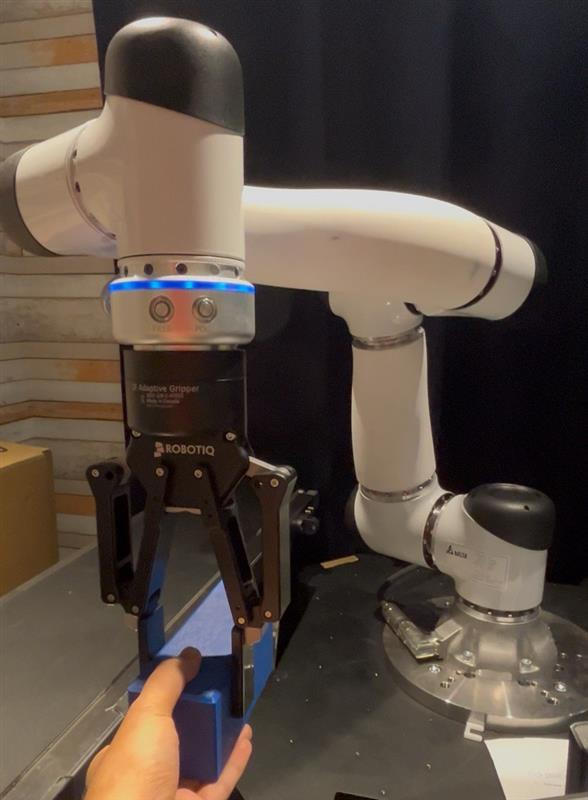
\includegraphics[width=5cm]{Thesis-report/Figures/pick.jpeg}
        \label{fig:pick}
    \end{minipage}
    \hfill
    \begin{minipage}{0.45\textwidth}
        \centering
        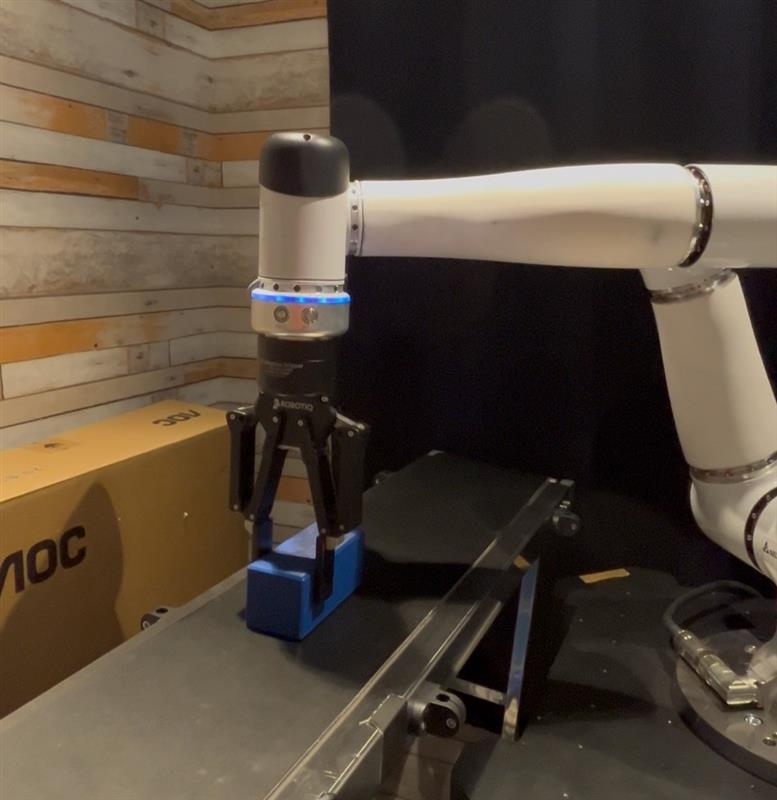
\includegraphics[width=6cm]{Thesis-report/Figures/picking.jpeg}
        \label{fig:picking}
    \end{minipage}
    \caption{Dynamic picking}
    \label{fig:gripper-combined}
\end{figure}


For the Dynamic picking, a typical construction site is needed, and quick, real-time modeling is necessary to support decision-making.  Thus, a quick 3D data collection and processing system is required for real-time modeling of a building site.  Only high-quality, rich 3D datasets of static objects are produced using laser scanners; a typical scan has millions of points.  Furthermore, real-time modeling is not practicable due to the slowness of data collection and processing.  Nevertheless, 3D range cameras provide an additional option by enabling wide-field-of-view, low-cost, automatic tracking and detection of both static and moving objects at frame rates higher than 1Hz (real-time).
The working happens in Dynamic can be as follows:\\

Initially, we pass the object through the running conveyor belt and trigger the camera, where we get the initial and final coordinates. We also calculate the timestamps to get the changes in time. Then we need to find the custom velocity, which can be calculated by dividing the change in position by and change in time.
When we pass the object through the conveyor belt, there is a change in position in the X axis, as this is a linear motion of movement. The change in the position of the object needs to be transferred to the robot, so that the robot can understand where it needs to come and pick the item from the conveyor belt. This can be compensated by using the following equation: \[ X = X_0 + v\cdot t \] where X0 is the initial position of the object. \\
where X is the final position of the object\\
v is the velocity / calibrated custom velocity in m/s\\
t is a change in time \\

\subsection{Coordinate Transformation:}
Many applications in manufacturing, construction, and vehicle automation and autonomy depend on the availability of 3D information.  Time-of-flight (TOF) sensors are getting cheaper and more accessible. They offer in-depth information at every pixel in addition to intensity.
The TOF sensor provides spherically-coordinated range data of the environment within its field of view.  As described in the following section, the spherical coordinates are transformed into Cartesian coordinates, with the origin of the coordinate system located at the camera's center.
 With the origin at a known reference point, the 3D point cloud in the camera coordinate system is converted to the belt coordinate system. \\

 The tests examine the capacity of TOF sensors to provide sensing for a robot tasked with handling goods traveling on a conveyor belt in an indoor scenario.  The range data is utilized to identify and calculate the dimensions of objects traveling along a conveyor belt.  The robot then receives the geometry and recognition data for additional action.  The findings suggest that TOF sensors have immediate potential for automating these kinds of applications.\\

 The coordinate transformation is necessary for two reasons:
 \begin{enumerate}
     \item  To enable the robot to be guided by the range camera's measurements, the robot and the camera must agree on a coordinate system.

    \item The z-axis is normal to the belt plane in the belt coordinate system.  By referring to points above the belt plane (z greater than 0) and inside the belt limits, this alignment of the coordinate axis makes it easier to extract item point clouds on the belt.
 \end{enumerate}
 \newpage
\subsection{Euler Angles:}\\
Euler angles can be used to parameterize the space of orientations. A universal orientation is expressed as a sequence of rotations along three mutually orthogonal axes in space when Euler angles are applied. In a Cartesian coordinate system, the x, y, and z axes are typically utilized. The rotations are frequently referred to as x-, y-, and z-rolls.To solve differential equations, Euler initially created Euler angles. The most popular technique for parameterizing the space of orientations is now the use of Euler angles. Euler angles can be used to parameterize the space of rotations if we decide to think of a rotation as the activity carried out to achieve a specific orientation. The rotation angles about the x, y, and z axes are denoted as { 1, { 2, and { 3, respectively.[20]
\subsubsection{Rotation matrices}\\
Euler angles are usually implemented using rotation matrices. There is an x rotation matrix, a y rotation matrix, and a z rotation matrix for every kind of roll. The position vector for the rotated point is obtained by multiplying the matrices by the position vector for a point in space. Although a rotation matrix is a 3 × 3 matrix, homogeneous 4 × 4 matrices are typically utilized in its place. The three roll matrices corresponding to the three Euler angles are multiplied to produce a general rotation. The generated matrix can be applied to the locations that need to be rotated and represents the general rotation. In most cases, matrix multiplication is not commutative. The fact that rotations in space do not commute fits in nicely with this. Lastly, it should be mentioned that the only implementation that effectively incorporates all common transformations—translation, scaling, shearing, and different projection transformations—is the use of homogeneous transformation matrices.[20]

\subsection{Quaternions:}\\
The second rotational modality uses quaternions and is defined by Euler's theorem. Given the lack of a comprehensive overview of the field and the fact that quaternions are not nearly as well-known as transformation matrices, we will first provide a historical perspective before delving deeply into quaternion mathematics.[20]
\newpage
\subsection{Object for picking}
We have used trapezoid for object picking 

\begin{figure}[h]
    \centering
    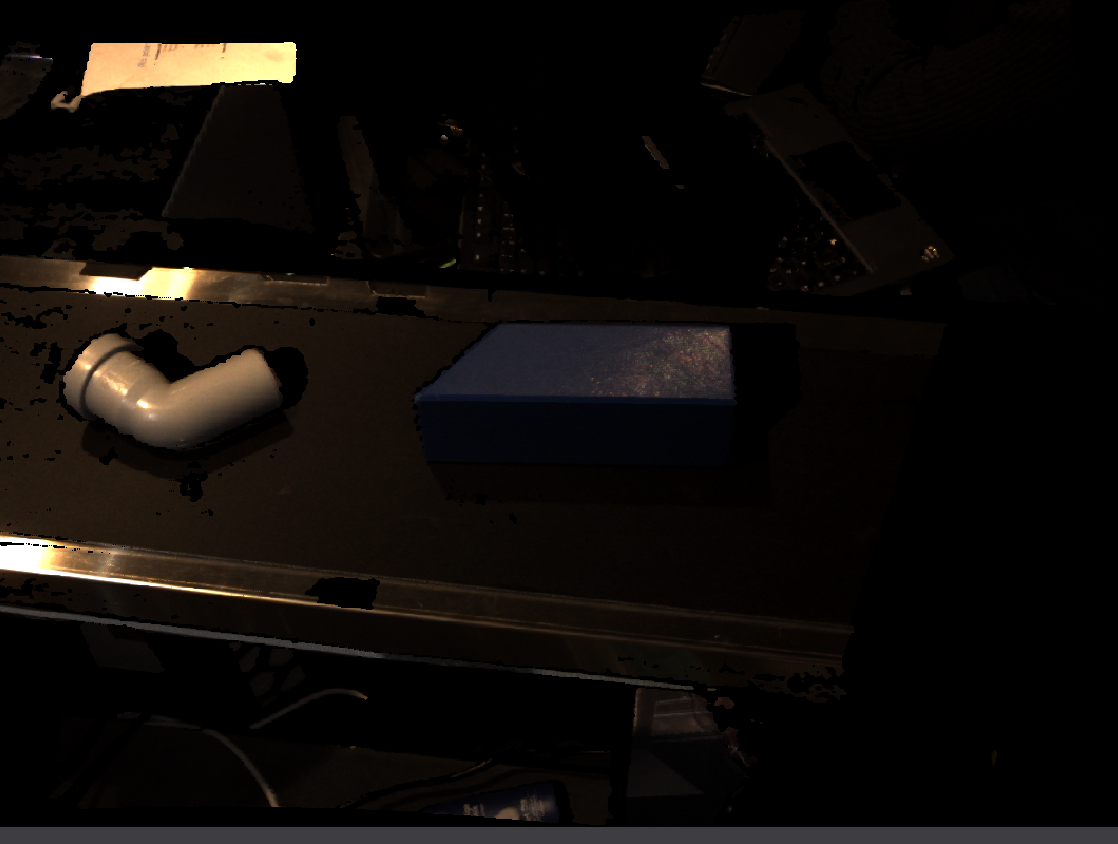
\includegraphics[width=6cm]{Thesis-report/Figures/two.png} 
    \caption{Trapezoid}
    \label{fig1.Photoneo Cmaera}
\end{figure}

\subsubsection{Trapezoid}
The trapezoid  is:\\

\centering
\begin{minipage}{0.38\textwidth} % Adjust width as needed
    \centering
    \includegraphics[width=8cm]{Thesis-report/Figures/trapezoid_stl.jpg} 
    \caption{STL file for Trapezoid object}
    \label{fig:trapezoid_stl}
\end{minipage}
\hfill
\begin{minipage}{0.28\textwidth} % Adjust width as needed
    \centering
    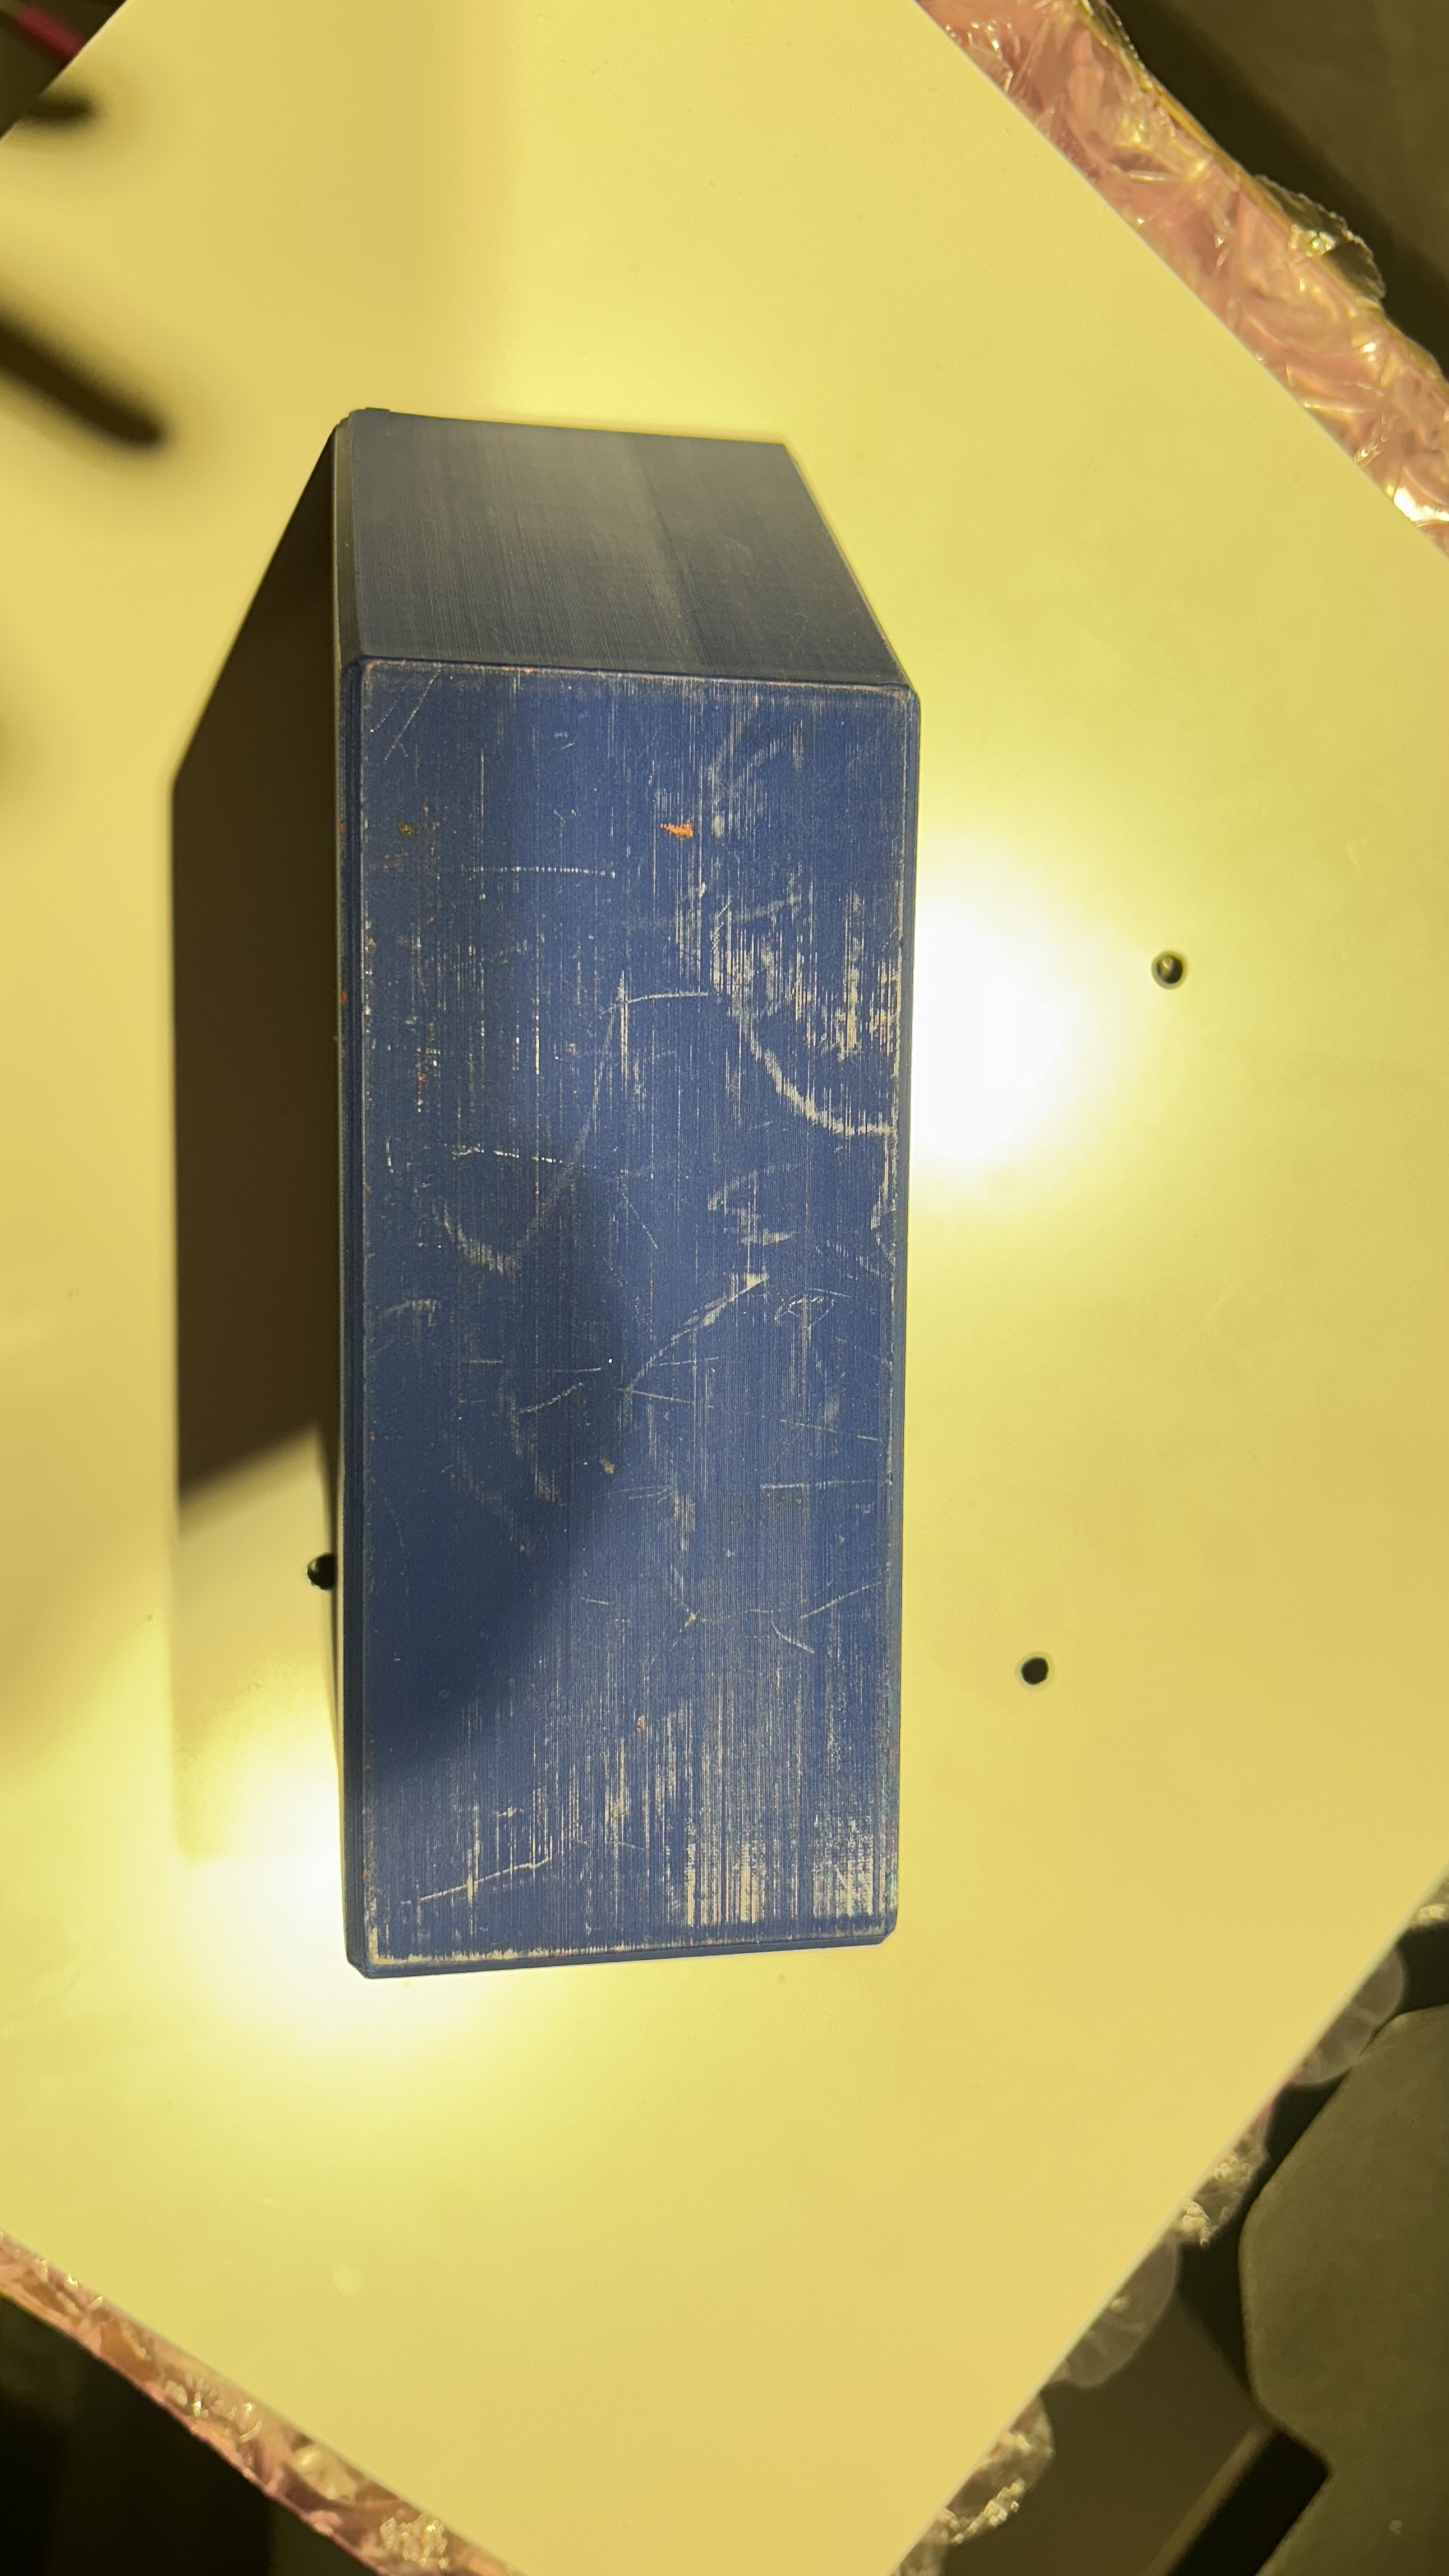
\includegraphics[width=3cm]{Thesis-report/Figures/trapezoid.png} 
    \caption{Trapezoid object}
    \label{fig:trapezoid}
\end{minipage} \\\\


The figure above shows the STL file of the trapezoid, which is used to pick up the object. While loading the STL file for the object, we will get the X, Y, and Z coordinates for the object.

\newpage
\begin{align}
    
\end{align}
\begin{flushleft}
\subsubsection{Conveyor Belt}
\begin{flushleft}
The conveyor belt is the main belt where we have to place the object, thereby putting the object into dynamic mode.[22]\\

The conveyor belt specification includes:\\
\begin{enumerate}
    \item The item model has Belt size: 59x7.8 in/1498.6x198 mm [22]
    \item Table Width: 9.9 in/ 252 mm [22]
    \item Load Capacity Limit: 82.67 lbs/37.5 kg [22]
    \item Material: 201 Stainless Steel [22]
    \item Product Weight: 40.79/18.5 kg [22]
    \item Conveyor belt speed: Bi-directional Variable speed, 28 m/min [22]
    \item Product Size: 58.86 x 14.17 x 35.91 in/1495 x 360 x 912 mm [22]
\end{enumerate}

\begin{figure}[h]
    \centering
{
        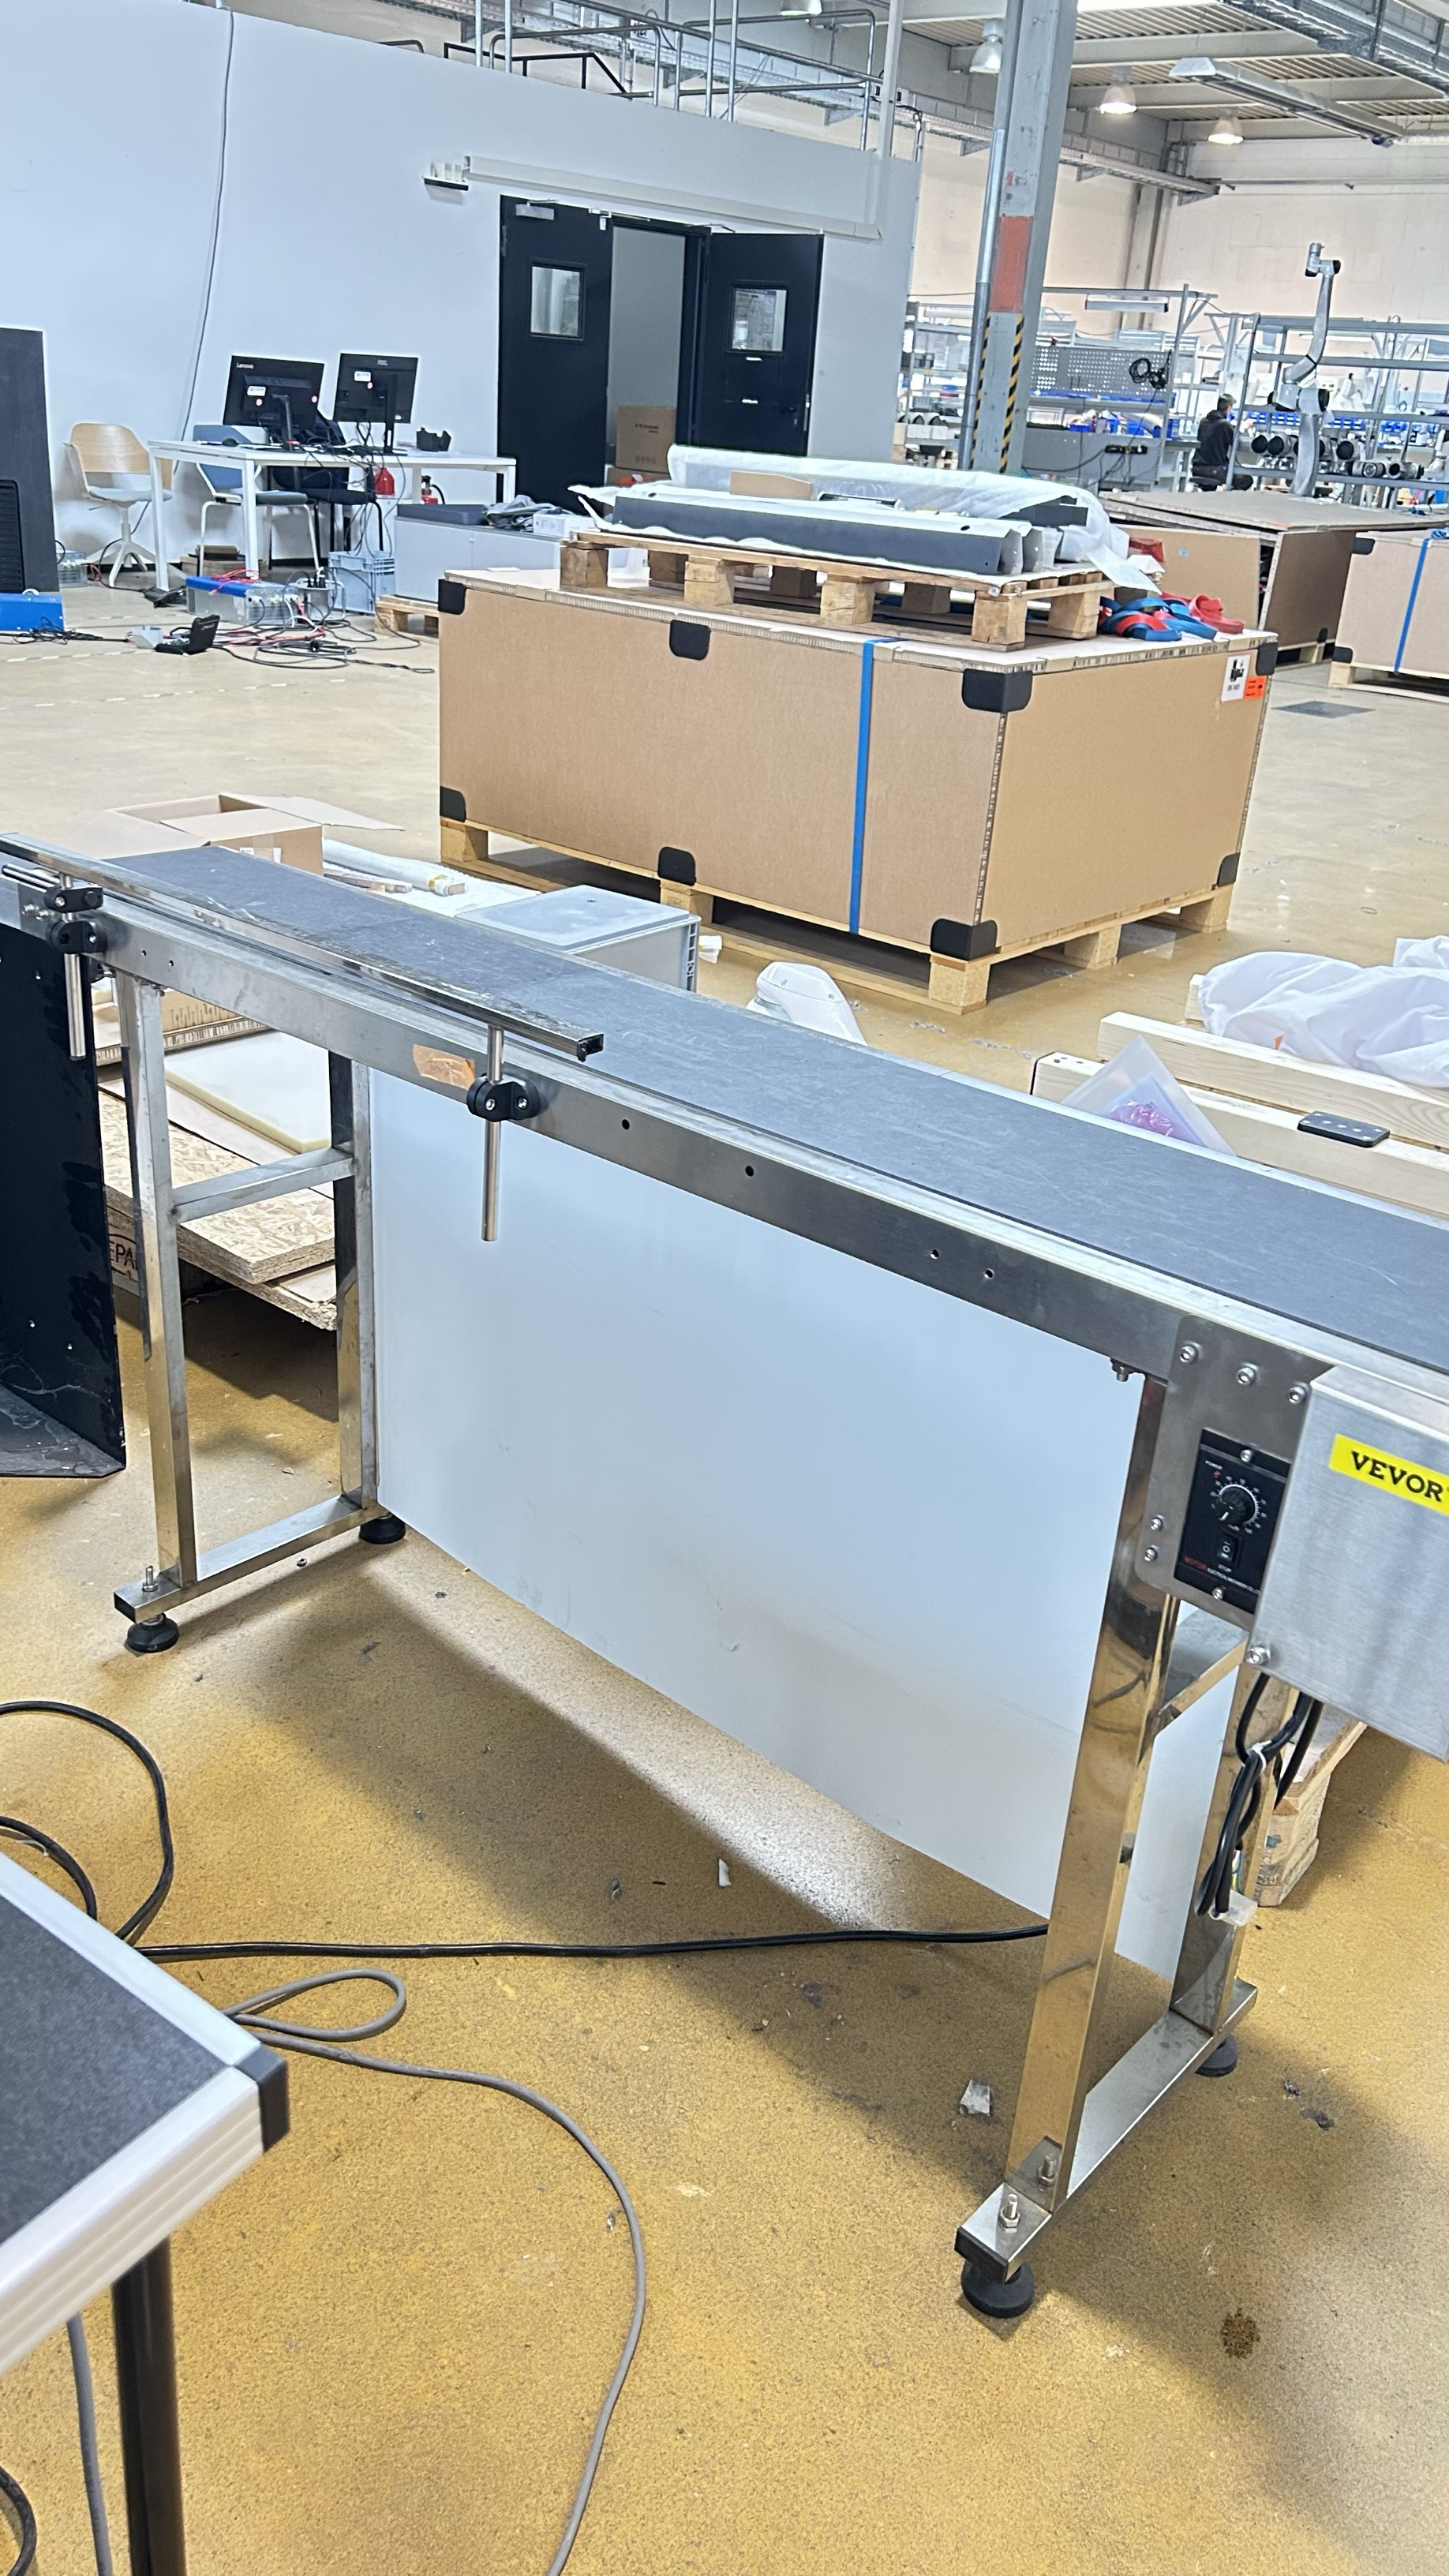
\includegraphics[width=5cm]{Thesis-report/Figures/CV belt1.jpeg}
        \label{fig:cv_belt1}
    }
    \quad
{
        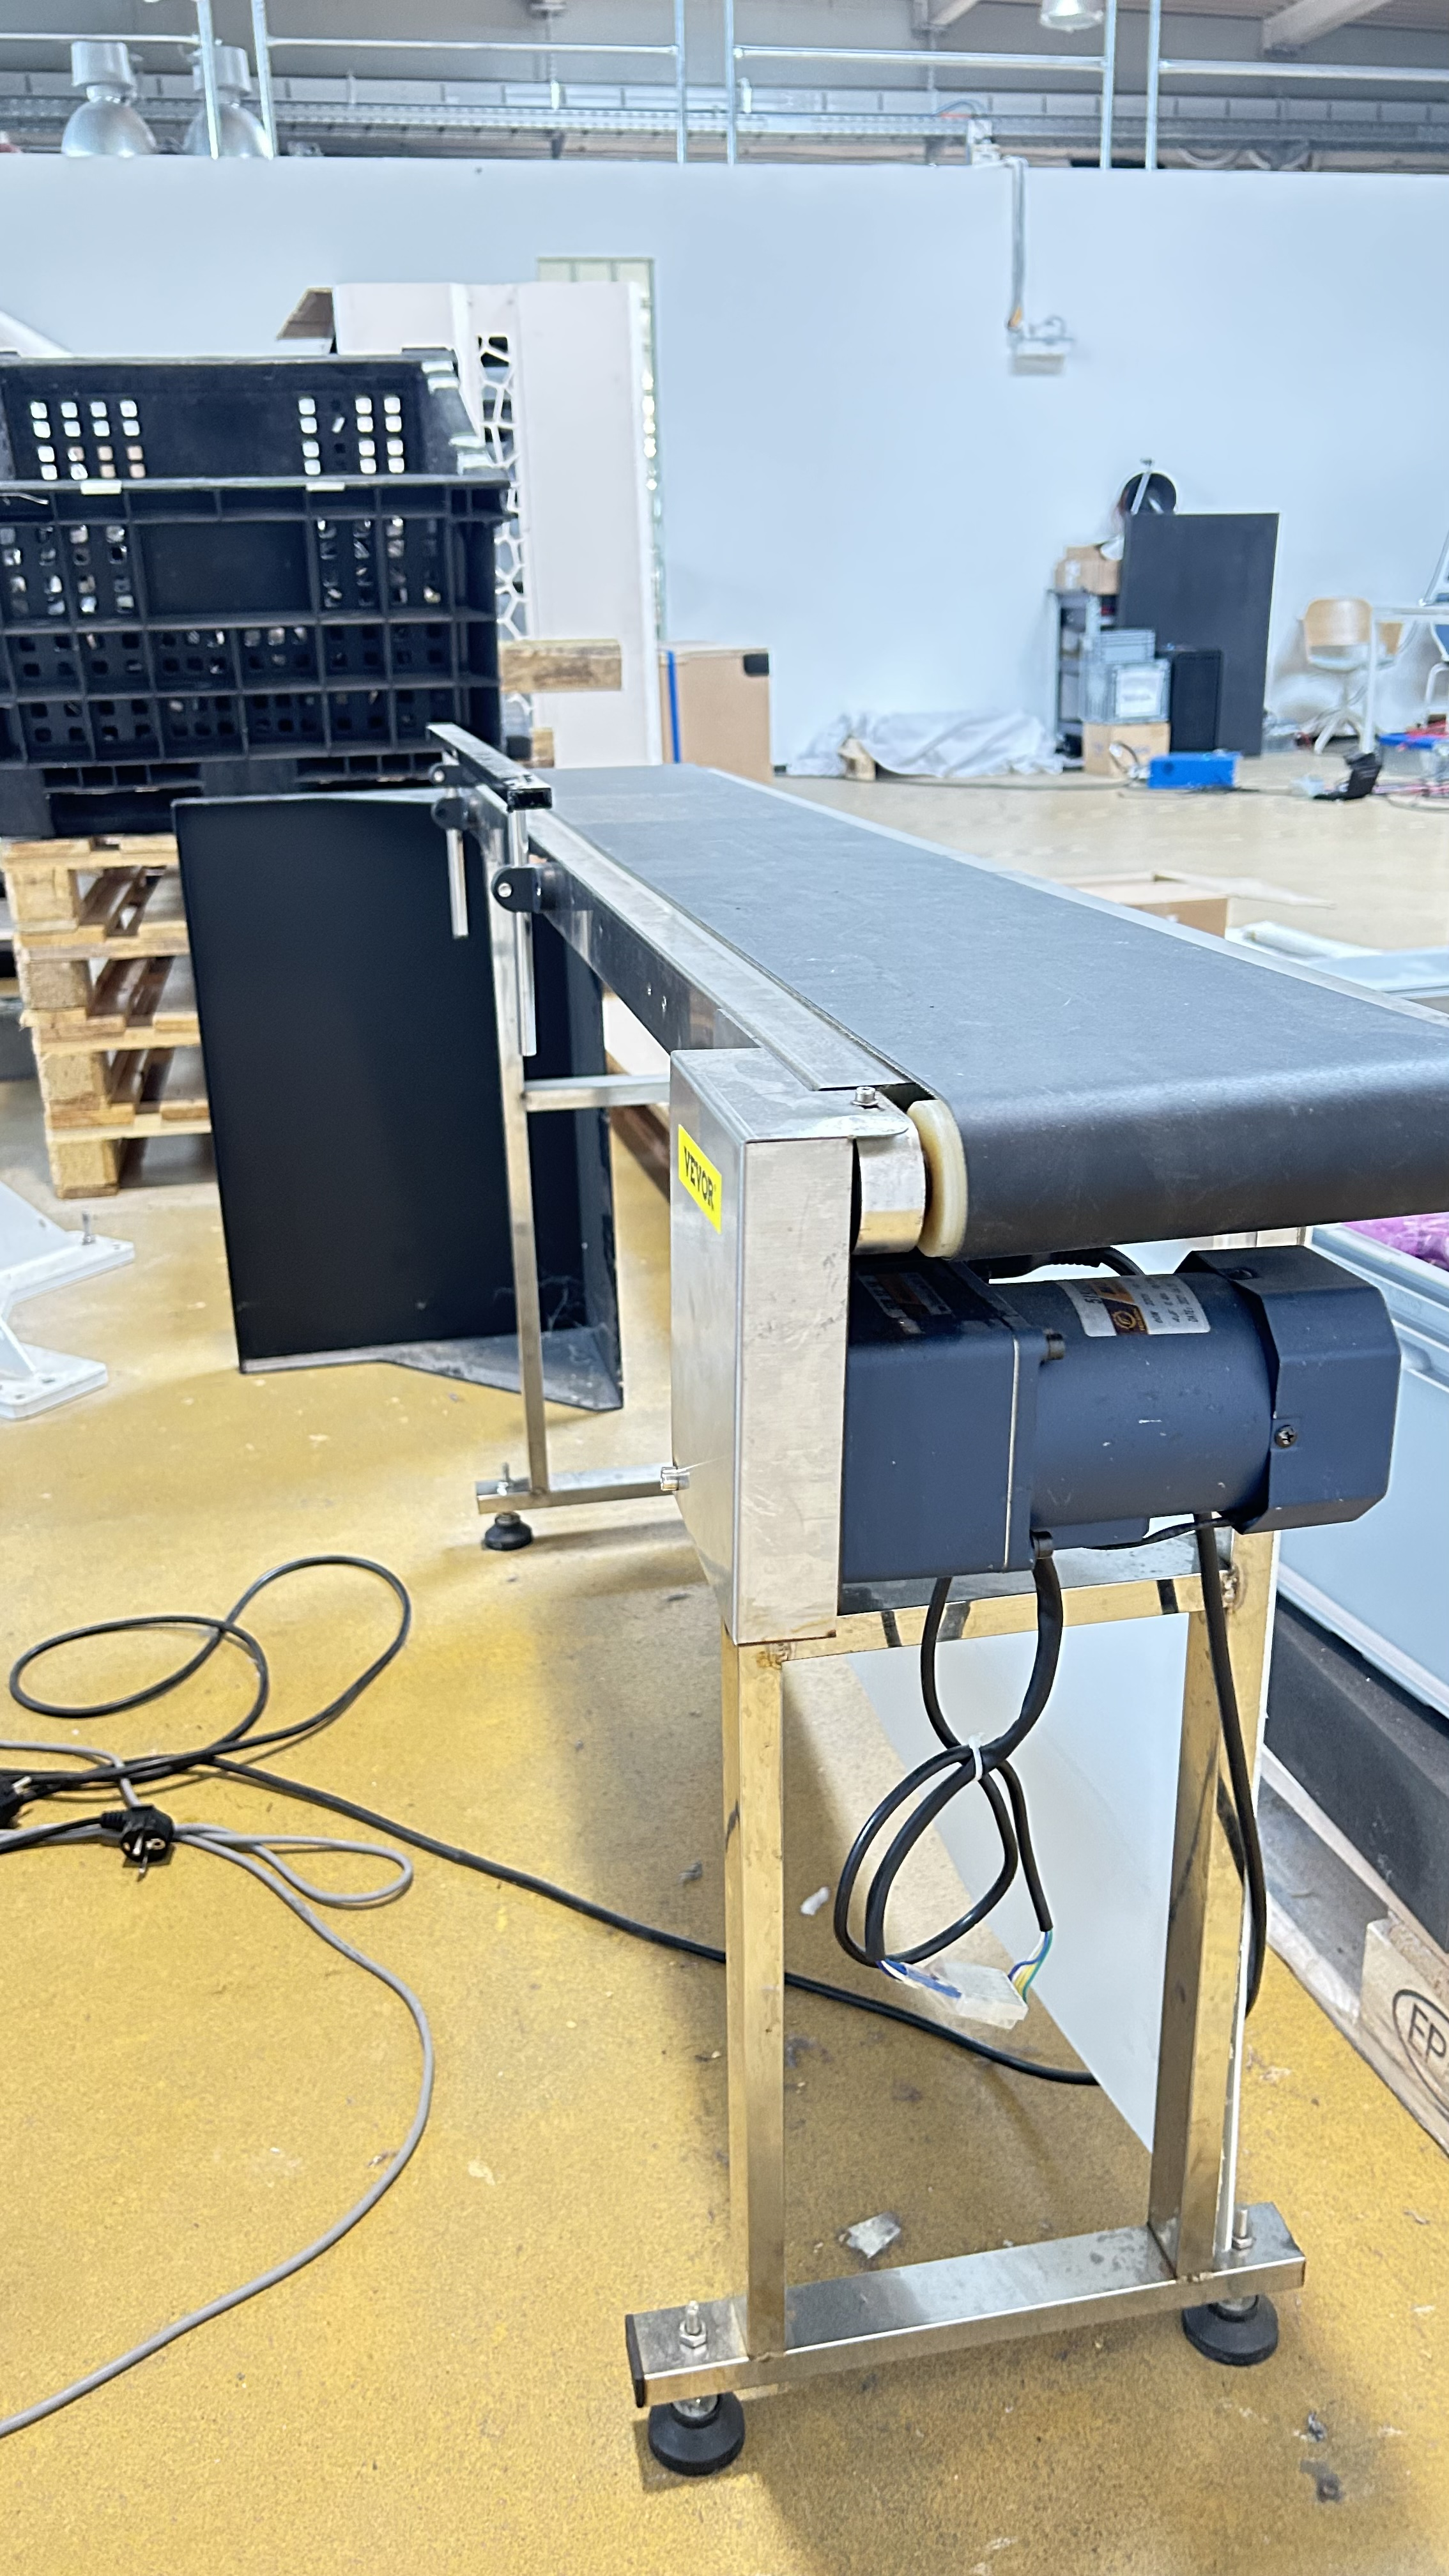
\includegraphics[width=5cm]{Thesis-report/Figures/CV_ belt2.jpeg}
        \label{fig:cv_belt2}
    }
    \caption{Images of the conveyor belt}
    \label{fig:conveyor_belt}
\end{figure}

The following figure shows the parts, which include: 

\begin{flushleft}
1. \textbf{Conveyor Belt:} The conveyor belt is the main surface that moves materials or products from one point to another. It always runs when the motor is on and effectively carries items of various shapes and sizes.[22]\\
\begin{flushleft}

\begin{flushleft}
2.	\textbf {Adjustment Lever:}
Function: The conveyor system can be adjusted thanks to this lever. It can be used to adjust the height, alignment, or tension of the belt to guarantee smooth operation and to suit various materials.[22]
\begin{flushleft}
3.	\textbf {Guardrail:}
Function: To stop goods from slipping off during transportation, guardrails are positioned along the conveyor belt's sides. It aids in safely guiding objects along the belt, particularly when working with slick or irregular objects.[22]\\

4.	\textbf {Motor:}
Function: The conveyor belt can move because of the motor's power. It drives the belt directly or via a gearbox and pulleys by converting electrical energy into mechanical energy.[22]\\
\begin{figure}[h]
    \centering
    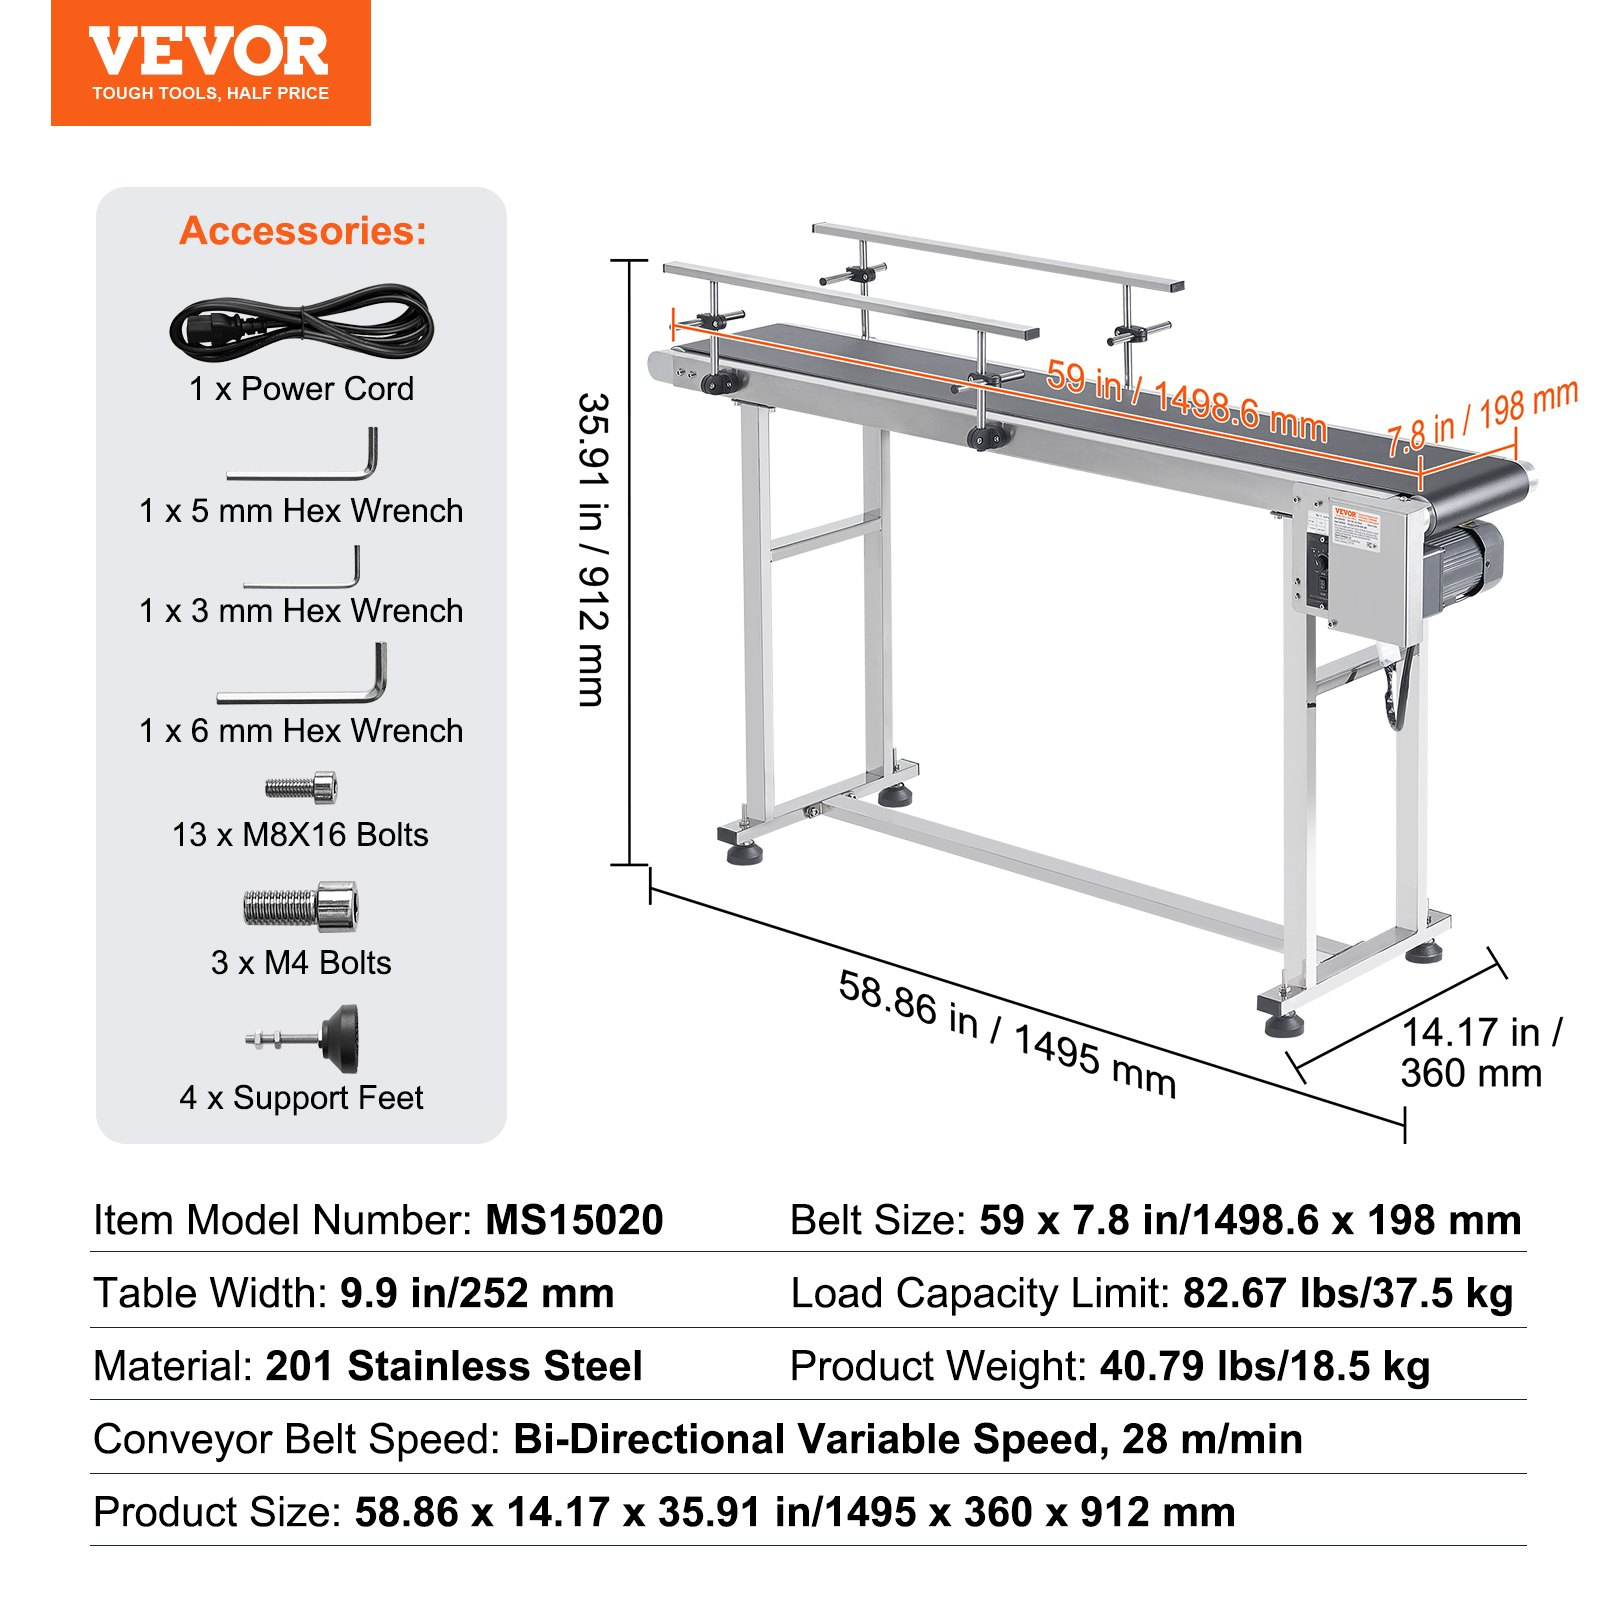
\includegraphics[width=6cm]{Thesis-report/Figures/belt_dimension.jpg}
    \caption{Conveyor belt with Details[22]}
    \label{fig1.Photoneo Cmaera}
\end{figure}

5.	\textbf {Control Panel:}
Function: Operators can oversee the conveyor's operation from the control panel. Switches, speed controls, emergency stop buttons, and other controls to modify the conveyor's direction, speed, and mode of operation may be included.[22]\\

6.	\textbf{Rubber Feet:}
Function: During operation, the rubber feet help absorb vibrations and stabilise the conveyor system. They also protect the floor from scratches and prevent the conveyor from sliding on smooth surfaces [22].\\

\begin{figure}[h]
    \centering
    \includegraphics[width=5cm]{Thesis-report/Figures/cvdimension.jpg}
    \caption{Conveyor belt with Dimensions[22]}
    \label{fig1.Photoneo Cmaera}
\end{figure}
\newpage
\subsection{Photoneo Camera-Web Interface}\\

For running the Solution request, after verifying that the environment complies with all necessary safety rules, Button Deploy launches the solution.[2]\\

\begin{figure}[h]
    \centering
    \includegraphics[width=10cm]{Thesis-report/Figures/deploy.jpg}
    \caption{Solution Deployment[2]} 
    \label{fig1.Photoneo Cmaera}
\end{figure}
Runtime requests from action clients are received and executed following the deployment of a defined solution.  The Action Request Client (Robot main software) and Photoneo 3D Sensors (vision systems) connection statuses can be viewed by the user. Additionally, it provides the ability to call a Scan request and a Get object request, as well as to halt or resume the deployed solution.[2]\\
The deployment page shows console logs that provide information about previous actions and occurrences, along with a visualiser that presents the following data:[2]

○	Real-time visualization of the captured 3D point cloud[2]
○	Localized objects rendered in colors corresponding to their status[2]
\begin{enumerate}
    \item Localized \colorbox{green}\\ 
    \item Being picked \colorbox{blue}\\
    \item Rejected \colorbox{red}\\
\end{enumerate}

○	Inspector tool for diagnostics of every localized object[2]

The web interface shows the image of the object being detected; initially, we load the STL file of the object to be captured by the robot. The red color indicates the object, and once the object turns green, the object coordinate will be indicated as quaternion values. After getting the quaternion values, these are transferred to the Robotic controller, which helps the robot to get into the desired target position.[2]\

\begin{figure}[h]
    \centering
    \includegraphics[width=12cm]{Thesis-report/Figures/web interface.jpeg} 
    \caption{Camera web interface}
    \label{fig1.Photoneo Cmaera}
\end{figure}

\begin{figure}[h]
    \centering
    \includegraphics[width=12cm]{Thesis-report/Figures/new.jpeg}
    \caption{Object detection with pipe }
    \label{fig1.Photoneo Cmaera}
\end{figure}
\newpage
 The above figure represents the web interface that includes the camera triggering the object placed in the workspace. The green section represents the area for the workspace, and the red section is the object to be picked up by the Robot. Using a TCP/IP client request connection in which the robot and camera connections are being established. For setting up the connection, the robotic controller and camera IP address (subnet) are made into the same, which helps in communication through a web interface.
\newpage
\begin{figure}[h]
    \centering
    \includegraphics[width=8cm]{Thesis-report/Figures/scanning volume.png} 
    \caption{Scanning Volume [18]}
    \label{fig1.Photoneo Cmaera}
\end{figure}
 The above figure shows the volume/area in which the Photoneo Camera is possible to scan the items and get the object poses. The top view shows the maximum FOV where the camera can reach the object to get the object coordinates, which includes 15m.\\

\newpage
\chapter{\section{\mbox{Results and Discussions }}{{\normalfont\fontsize{14}{16}\bfseries}}
\subsection{Robot TCP Speed vs Conveyor Speed}
The below figure shows the results that is obtained while picking the items on a moving conveyor belt speed (m/s) concerning the Robot speed.\\
\label{Literature}
\begin{figure}[h]
    \centering
    \includegraphics[width=12cm]{Thesis-report/Figures/conveyor_speed vs Robot tcp speed.png} 
    \caption{Robot TCP Speed vs Conveyor Speed}
    \label{fig1.Photoneo Cmaera}
\end{figure}\\
\subsection{Success Rate vs Conveyor Speed}
During the dynamic picking testing, I tested the picking of the Trapezoid object with the pipe to have a comparison for getting some results. The below figure shows the results that are obtained while placing the items that include the trapezoid and pipe on a moving conveyor belt speeds (m/s) concerning Success rates.\\
\begin{figure}[h]
    \centering
    \includegraphics[width=12cm]{Thesis-report/Figures/conveyor_speed vs success_rates.png} 
    \caption{Success Rate vs Conveyor Speed}
    \label{fig1.Photoneo Cmaera}
\end{figure}\\
\subsection{Average Pick Time vs Conveyor Speed}
The below figure shows the results obtained while placing the items on a moving conveyor belt speed (m/s) concerning the Avg pick-up time.\\
\begin{figure}[h]
    \centering
    \includegraphics[width=12cm]{Thesis-report/Figures/conveyor_speed vs avg pick_up_time.png} 
    \caption{Average Pick Time vs Conveyor Speed}
    \label{fig1.Photoneo Cmaera}
\end{figure}\\
\subsection{Average Pick Time vs Lighting condition}
The figure below shows the results that are obtained while placing the items that include the trapezoid and pipe with an Avg pick-up time vs. lighting conditions.\\
\begin{figure}[h]
    \centering
    \includegraphics[width=12cm]{Thesis-report/Figures/Picking_time vs item_type.png} 
    \caption{Average Pick Time vs Lighting condition}
    \label{fig1.Photoneo Cmaera}
\end{figure} \\


\chapter{\section{\mbox{Conclusions and Future Prospects}}{{\normalfont\fontsize{14}{16}\bfseries}}
\label{Literature}

\subsection{Conclusion}


Conveyor tracking systems have become indispensable components in modern industrial and logistic operations, facilitating the seamless movement of goods across various stages of production, storage, and distribution. Over the years, advances in technology have significantly improved the efficiency, accuracy, and reliability of these systems. Key achievements in conveyor tracking include:

\begin{itemize}

\item Enhanced Automation and Integration: The integration of conveyor tracking with other automated systems, such as Warehouse Management Systems (WMS) and Enterprise Resource Planning (ERP) software, has streamlined operations, reduced manual intervention, and minimized errors.

 \item Real-Time Monitoring and Data Analytics: Modern conveyor tracking systems leverage sensors, IoT devices, and advanced analytics to provide real-time information on the movement of goods. This capability enables proactive decision making, predictive maintenance, and optimized resource allocation.

\item Improved Accuracy and Efficiency: Innovations in tracking technologies, including barcode scanners, RFID tags, and machine vision, have significantly improved the accuracy of item identification and tracking, leading to a reduction in loss, theft, and misplacement of goods.

\item Scalability and Flexibility: Contemporary conveyor systems are designed to be highly scalable and adaptable, allowing businesses to adjust their operations based on fluctuating demand and changing market conditions without substantial infrastructure overhauls.

\item Sustainability and Energy Efficiency: Advances in conveyor technology have also focused on energy efficiency and sustainability, incorporating energy-saving motors, regenerative braking systems, and eco-friendly materials to reduce the environmental footprint of conveyor operations.
\end{itemize}
\newpage
\subsubsection{Future Scope }

The future of conveyor tracking is poised to be shaped by continued technological innovations and evolving industry demands. Potential developments and areas for growth include:

\begin{itemize}

\item Artificial Intelligence and Machine Learning: Integrating AI and ML algorithms can enhance predictive maintenance, optimize routing, and improve overall system intelligence. These technologies can analyze vast amounts of data to identify patterns, predict failures, and recommend operational adjustments in real time.

\item Advanced IoT Integration: The proliferation of IoT devices will further enhance the connectivity and interoperability of conveyor tracking systems. Enhanced IoT integration will enable more granular monitoring, improved data collection, and seamless communication between disparate systems and devices.

\item Augmented Reality (AR) and Virtual Reality (VR): AR and VR technologies can revolutionize training, maintenance, and operational planning. For instance, maintenance personnel can use AR glasses to receive real-time guidance and overlays while servicing conveyor systems, reducing downtime and improving efficiency.

\item Blockchain for Enhanced Security and Transparency: Implementing blockchain technology can provide immutable records of product movement and handling, enhancing traceability, security, and transparency throughout the supply chain.

\item Robotic Integration and Automation: The integration of robotics with conveyor tracking systems can further automate material handling processes. Collaborative robots (cobots) can work alongside conveyor systems to perform tasks such as sorting, packaging, and inspection with greater precision and speed.

\item Sustainability and Green Technologies: Future conveyor systems will increasingly incorporate sustainable practices, such as the use of renewable energy sources, recyclable materials, and energy-efficient designs. Innovations aimed at reducing waste and minimizing the environmental impact will become paramount.

\item Enhanced user interfaces and human-machine interaction: The development of more intuitive and user-friendly interfaces will improve the interaction between operators and conveyor tracking systems. Voice-controlled interfaces, touchless controls, and advanced visualization tools will make system management more accessible and efficient.

\item Edge Computing and Enhanced Processing Capabilities: Implementing edge computing will allow data processing to occur closer to the source, reducing latency and improving the responsiveness of conveyor tracking systems. This will be particularly beneficial for real-time applications and environments with limited connectivity.

\item Customization and Modular Designs: Future conveyor tracking systems will offer greater customization and modularity, allowing businesses to tailor systems to their specific needs without extensive redesigns. Modular components can be easily added, removed, or reconfigured to adapt to changing operational requirements.

\item Enhanced cybersecurity measures: As conveyor tracking systems become more connected and reliant on digital technologies, ensuring robust cybersecurity will be critical. Future developments will focus on implementing advanced security protocols, encryption methods, and intrusion detection systems to protect against cyber threats.
\end{itemize}

\newpage

\chapter{\section{\mbox{References}}{{\normalfont\fontsize{14}{16}\bfseries}}

\begin{thebibliography}{99}

\bibitem{ref1}
Adil Shahzadi, Xueshan Gao , Awais Yasin, Kamran Javed, Syed Muhammad Anwar, \textit{A Vision-Based Path Planning and Object Tracking Framework for 6-DOF
Robotic Manipulator}, IEEE, 2020
\bibitem{ref2} Locator Studio Manual, Photoneo
\bibitem{ref3}
Guor-Yieh Luo, Ming-Yang Cheng, Chia-Ling Chiang\textit{Vision-Based 3-D Object Pick-and-Place Tasks of Industrial Manipulator}, National Cheng Kung University,
\bibitem{ref4}
P. Wunsch and G. Hirzinger,\textit{Real-Time Visual Tracking of 3-D Objects with Dynamic Handling of Occlusion}, German Aerospace Research Establishment - DLR
Institute for Robotics and System Dynamics
82230 Wessling, Germany, IEEE,1997
\bibitem{ref5} Mar Arif, Matt Marshall, Wayne Daley, Patricio A. Vela, Jochen Teizer, Soumitry J. Ray,
and John Stewart\textit{TRACKING AND CLASSIFYING OBJECTS ON A
CONVEYOR BELT USING TIME-OF-FLIGHT CAMERA},7th International Symposium on Automation and Robotics in Construction (ISARC 2010)
\bibitem{ref6}Dong Sun, Member, IEEE, and James K. Mills\textit{Adaptive Synchronized Control for Coordination
of Multirobot Assembly Tasks}, IEEE,2002
\bibitem{ref7}Amit Agrawal, Yu Sun, John Barnwell, Ramesh Raskar\textit{Vision-guided Robot
System for Picking
Objects by Casting
Shadows}, the International Journal of Robotics Research,2010
\bibitem{ref8}Hüseyin N. Karaca and Cüneyt Akınlar\textit{A Multi-camera Vision System for Real-Time Tracking
of Parcels Moving on a Conveyor Belt}, Department of Computer Engineering, Anadolu University, Eskisehir, Turkey
\bibitem{ref9}Yizhe Zhang*, Lianjun Li†, Michael Ripperger‡, Jorge Nicho‡, Malathi Veeraraghavan* and Andrea Fumagalli†\textit{Gilbreth: A Conveyor-Belt Based Pick-and-Sort
Industrial Robotics Application}, IEEE,2018
\bibitem{ref10}Adrian-Vasile Duka*\textit{Neural network based inverse kinematics solution for trajectory
Tracking of a robotic arm}, The 7th International Conference Interdisciplinarity in Engineering (INTER-ENG 2013)
\bibitem{ref11}Wisam T. Abbood1, Hiba K. Hussein1 and Oday I. Abdullah\textit{INDUSTRIAL TRACKING CAMERA AND PRODUCT VISION DETECTION SYSTEM}, Journal of Mechanical Engineering Research and Developments (JMERD: 1024-1752,2019
\bibitem{ref12}Ik Sang Shin1, 3, Sang-Hyun Nam2
, Hyun Geun Yu3, Rodney G. Roberts, Seungbin B. Moon\textit{Conveyor Visual Tracking using Robot Vision}, ResearchGate, 2006
\bibitem{ref13}Chen-yu Wang\textit{Conveyor tracking using adept robot with vision guidance system}, 1996
\bibitem{ref14}T. H. Park and B. H. Lee\textit{An Approach to Robot Motion Analysis and
Planning for Conveyor Tracking}, IEEE,1992
\bibitem{ref15}Tomas Kovacovsky & Jan Zizka\textit{Vision Award}, Photoneo s.r.o.
Germany, 2018.
\bibitem{ref16}Yangtao Ge, Chen Yao, Zirui Wang, Haoran Kang, Wentao Zhang, and Jing Wu, Automatic Extrinsic Calibration for Lidar-Photoneo
Camera Using a Hemispherical Calibration Board,2023 9th International Conference on Mechatronics and Robotics Engineering,
\bibitem{ref17}Miguel Fernandez, Scan to 3D Model and parametric data system implementation, Turku University of Applied Sciences, Bachelor of Information and Communications Technology, 2021.
\bibitem{ref18} Motion Cam  -3D Color Map Datasheet
\bibitem{ref19} Robot Manipulation through Inverse Kinematics, Abdullah Aamir Hayat,Abdullah Aamir Hayat, Abdullah Aamir Hayat, Indian Institute of Technology Delhi.
\bibitem{ref20} Quaternions, Interpolation and Animation,Erik B Dam, Martin Koch , Martin lillholm, Department of Computer Science University of Copenhagen, Denmark, 1998.
\bibitem{ref21} Locator studio setup, Photoneo

\bibitem{ref22} https://eur.vevor.com/belt-conveyor-c_10439 srsltid=AfmBOoqNYgY4dkBQihCa9ItoNIpgXAC6e39Atuqhn0fdtybn8S4CvWio


\end{thebibliography}




\end{document}


\addcontentsline{toc}{section}{Abstract} 


\pagenumbering{arabic}
\setcounter{page}{1}
\raggedright
\chapter{\section{\mbox{Introduction}}{\normalfont\fontsize{14}{16}\bfseries}}
\label{introduction}
It was the capacity of labor that propelled humanity forward, shaping the evolution of civilization and moulding its contours. In the modern world contemporary societies emerged as hybrid environments where the physical world intertwined seamlessly with digital. Human interaction found new means when virtual communication got advanced, while artificial intelligence is standing shoulder to shoulder with natural intelligence. 

The tools are also being evolved at this time. The tools are no longer bounded in human hands and they are not guided solely by human will. Artificial intelligence enabled autonomy for these tools granting the machines the power to operate independently, make decisions, and chart their own course. As the world stood on the edge of this paradigm shift, the need for a deeper understanding of this technology became important.

Researchers, policymakers businesses, and society at large, all joined hands recognizing technology in all its brilliance,must remain a servant to humanity. The tool must enhance work preserving its current dual nature well spring for creation and a conduit for human fulfillment. After the pandemic COVID-19 hit the world the evolution of automation and AI was accelerated, reshaping warehouses, manufacturing plants, grocery stores, and call centers. The emergence of artificial intelligence rewrote the structure of human life transferring the way we were toiled, the way we learned and the way we structured our businesses and work. The world of robotics and automation ushered in a new era of collaboration. Man and machine are now sharing tasks, space, and even rhythm of creation.\cite{author1}
 
 Four repeated modes of collaboration of humans and robots emerged, These modes are named  co-existence, sequential collaboration, co-operation, and responsive collaboration complimenting each other's strength as shown in Figure\ref{Fig:1l}.
 \begin{figure}[H]
    \centering
    \includegraphics[width=0.8\linewidth]{Figures/Human Robot collaboration.png}
    \caption{Types of Human Robot Collaboration in industrial environment\cite{author3}}
    \label{Fig:1l}
\end{figure}
As the wheel of progress is spinning faster robotics and AI is being advanced in tandem with Big Data, Industry 4.0, and the Internet of Things. The possibilities expanded, expanding far beyond the repetition of modes, technical configurations multiplied, each tailored to the specific demands of tasks, robots, collaboration styles, and production domains.

The integration of collaborative robot systems is a significant leap forward in industrial environments. With careful consideration of the human element, organizations can harness the full potential of this technology, redefining how humans and robots collaborate for increased productivity and safety.

 The International Organization of Standardization (ISO) defines a robot as an “automatically controlled, reprogrammable multipurpose manipulator, programmable in three or more axes, which can be either fixed in place or mobile for use in industrial automation applications” .\cite{author2}
 
 The emerged hybrid production systems aim to alleviate stress and workload blending the strengths of humans and robots. Safety became the cornerstone as robots gained the ability to sense and respond to their environment. Robots can now detect the touch of human hands, adapt to the presence of human workers and even anticipate their motions and conversations by integration of AI in robotics enhancing the safety of Human robot interaction. 
 
 Human-robot interaction is a critical aspect of collaborative robot systems. It encompasses verbal and non-verbal communication, visual information, and gestures, all of which contribute to effective collaboration. In manufacturing, where tasks are often iterative and involve physical interaction, compliance with human states and intent is paramount. While substantial progress has been made in safety within Human robot interaction, challenges remain, particularly in achieving predictability. Designing robots to be tools that humans can understand and control is crucial. This requires formal conditions for system observability and controllability, as well as an understanding of the human's ability to control complex systems.\cite{author3}

While EN ISO 10218 part 1 and 2  were amended in 2011 there were safety measures suggested for human-robot collaboration in the collaborative cell this lead to an exponential rise in the research area of HRC.
Later in ISO/TS 15066, the limiting of forces in different type of robot movement and the design of the robot cells in a safe way were described for collaborative operations of robot with human, but AI integration and introducing cognitive abilities for a collaborative robot is not encompassed in this standards and technical specification.

The research questions we try to address through this thesis are 
What are the potential safety risks associated with AI-Integration in human-robot collaborative environments? How do AI-driven systems interact with other robotic functionalities, and what are the implications for overall system performance? What could be a risk analysis technique for AI-integrated robotic systems? What measures can be taken to ensure seamless integration of AI into lightweight cobots?

We try to answer these questions by studying perception and perception-based application in robotics.
Perception is one technology that is integrated into the robots, which enables the robots to understand their surroundings. Perception allows the robot to identify work material, human co-workers and the dynamic environment in which the robot is. AI-based grasping is one collaborative operation of the robot which can be derived from perception. The robot can grasp an object and pass to humans or humans can work on one object and then the robot picks it up or vice versa.

A process Failure Mode Effective Analysis on AI-based grasping is done in this thesis extending it with System Theory Process Analysis. AI-based grasping algorithms are studied and possible failures of these algorithms are viewed.The Hazard and Risk assessments are based on ISO/TS 12100, keeping in mind the EN ISO 10218-1,2:2011 and the technical specification ISO/TS 15066. 

To increase the reliability of the perception algorithm that induces grasping, different methods are proposed as the result of the thesis. In light of the results from this analysis of risk and hazards a safety framework is formulated for AI-based grasping, which can be taken into consideration, for a generic safety standard for the integration of artificial intelligence in robots.

\newpage
\documentclass[12pt]{article}
\usepackage{graphicx} % Required for inserting images
\usepackage[a4paper, top=2.5cm, bottom=2.5cm, left=2.5cm, right=2.5cm]{geometry}

\usepackage{babel}
\usepackage{float}
\usepackage{ragged2e}
\usepackage{rotating}
\usepackage{multirow}
\usepackage{tabularx}
\usepackage{lscape}
\graphicspath{ {figures/} }
\usepackage{array}
\usepackage{eso-pic,xcolor}
\usepackage{hyperref}
\usepackage{longtable}
\usepackage{booktabs}
\usepackage{array}
\usepackage{wrapfig}
\usepackage{changepage}
\usepackage{enumitem}
\usepackage[colorlinks=true, linkcolor=blue]{hyperref}


\newcommand\AtPageUpperRight[1]{\AtPageUpperLeft{
   \makebox[\paperwidth][r]{#1}}}

\begin{titlepage}

\begin{center}
    \vspace{-1cm} % Adjust this value if you want to move the image up or down
    \includegraphics[width=8cm]{Figures/th-deggendorf.png} % Centered image
    \vspace{1cm} % Space after the image
    
    \textbf{Master Thesis}{\normalfont\fontsize{14}{16}\bfseries}
    
    \vspace{0.7cm}
    
    \mbox{Deggendorf Institute of Technology, Deggendorf}
    
    \vspace{0.5cm}
    \mbox{Faculty of Mechanical and Mechatronics Engineering}
    
    \vspace{0.5 cm}
    
    \mbox{Master Mechatronics and Cyberphysical Systems}
    
    \vspace{4.0 cm}
    
    {Objektverfolgung mit 3D-Machine-Vision-Kamera für Industrieroboter}
    
    \vspace{0.5 cm}
    
    \textbf{Object Tracking using 3D Machine Vision Camera for Industrial Robots}
    
    \vspace{0.5 cm}
    
    \mbox{Master Thesis to obtain Academic Degree}
    
    \vspace{0.5cm}
    
    \textbf{Master of Engineering(M.Eng)}
    
    \vspace{1.5 cm}
    
    \mbox{submitted by: Midhun Eldose, 22101196}
    
    \vspace{0.5 cm}
    
    \mbox{first examiner: Prof. Ginu Paul Alunkal}
    
    \vspace{1.5 cm}
    
    \mbox{Deggendorf, 30.05.2025}

\end{center}
\end{titlepage}

\begin{titlepage}
 \makebox[\paperwidth][r]{#1}


\begin{center}

\vspace{0.5cm}

  \textbf{Confidential Disclosure Agreement}{\normalfont\fontsize{14}{16}\bfseries}
   
   \vspace{0.5 cm}
    
   \mbox{between}
   
   \vspace{0.5 cm}
   
   \textbf{Deggendorf Institute of Technology}{\normalfont\fontsize{14}{16}\bfseries}
   
   \vspace{0.2 cm}
   
   \mbox{Campus Deggendorf}
   
   \vspace{0.2 cm}
   
   \mbox{Dieter-Görlitz-Platz 1, }
   
    \vspace{0.2 cm}
    
   \mbox{94469, Deggendorf}
   
   \vspace{2.5 cm}
    
   \mbox{Faculty of Mechanical Engineering and Mechatronics}
    \vspace{0.2 cm}
    \mbox{Major: Mechatronics and Cyberphysical Systems}

    \vspace{0.5 cm}

    \mbox{ Prof. Ginu Paul Alunkal}

    \vspace{0.5 cm}

     \mbox{ (in the following "Deggendorf Institute of Technology")}

     \vspace{0.5 cm}
     
     \mbox{ and}

     \vspace{0.5 cm}

     \mbox{Midhun Eldose}
       \vspace{0.5 cm}

     \mbox{ (in the following "NEURA Robotics GmbH") }
     
     \vspace{0.5 cm}

     \mbox{ (in the following singularly and jointly "Contractual Partner") }

\end{center}
      
      \vspace{1.5 cm}
      
     \raggedright
     \textbf{Preamble}

    
    \vspace{0.5 cm}
     
     The Deggendorf Institute of Technology supervises an examination paper with the topic of\textbf{ Object Tracking using 3D Machine Vision Camera for Industrial Robots}

     \vspace{0.5cm}
     
     \mbox{}

     \vspace{0.5cm}
\begin{center}
    (in the following "examination paper"), In which, among other things, confidential 
     information of the company is processed. Simultaneously, confidential information was 
    also shared with the company in the context of supervision by the Deggendorf Institute of Technology.
\end{center}

\end{titlepage}

\newpage
\linespread{1.5}
\raggedright
\textbf{Declaration}

\vspace{0.5cm}

\mbox{Name of the Student: Midhun Eldose}

\vspace{0.5cm}

\mbox{Name of the first Examiner:  Prof. Ginu Paul Alunkal }

\vspace{1 cm}

\mbox{Title of master thesis:}

\vspace{0.5 cm}

Object Tracking using 3D Machine Vision Camera for Industrial Robots
\vspace{1.5 cm}

 I hereby declare that I have written this thesis independently. I have not submitted it for any other examination purposes. I have not used other references or materials than those mentioned in the bibliography, and I have marked all literal analogous citations.

 \vspace{1.5 cm}
\raggedright
Deggendorf,30.05.2025
\hspace{4 cm}
Signature of the student:


\linespread{1.5}
\pagenumbering{arabic}
\newpage

\begin{document}

\newpage
\tableofcontents
\newpage
\listoffigures
\addcontentsline{toc}{section}{List of Figures}
\newpage
\listoftables
\addcontentsline{toc}{section}{List of Tables}
\newpage
\raggedright
\newpage
\raggedright
\addcontentsline{toc}{section}{Acknowledgement}
\begin{center}
    \textbf{Acknowledgement}
\end{center}
    \raggedright

    I am highly indebted to NEURA Robotics GmbH, Metzingen, for their guidance and constant supervision, as well as for providing necessary information and resources for the Master's thesis and for the support in completing the report

    \vspace{1cm}
    
    I express my special gratitude to Dr.Sugeeth Gopinathan (Head of Software Strategy), Dr.Phuong Nguyen (Software Application Expert), Mr. Norman Kohler (Senior Robotics Engineer), Mr. Amarnath Reddy Bana (Group Lead), and Mr. Florian Schnös (ProduktManager Software) for instructing, providing information about how tasks are to be done and the flow of work, and guiding me for the thesis. In addition to that, I also thank all the members for their guidance and keen support at various stages of my thesis.

    \vspace{1cm}

    I am very grateful to my academic guide, Mr. Ginu Paul Alunkal, for his full support and encouragement. I owe him for his timely guidance, suggestions, and very constructive criticism, which contributed immensely to the evolution of my thesis.
    
    \vspace{1.5 cm}
    
    \raggedleft
    Midhun Eldose


\newpage
\begin{document}

\begin{abstract}{\normalfont\fontsize{14}{16}\bfseries}

The tracking of the conveyor using collaborative robots equipped with vision cameras represents a significant advancement in modern production. This innovative approach enables robots to dynamically interact with moving goods on conveyor belts, enhancing efficiency, precision, and adaptability. Using vision cameras, cobots can accurately detect, locate, and track objects in real-time, accommodating changes in shape, speed, and orientation. The integration of vision technology allows robots to perform tasks such as sorting, assembly, and pick-and-place operations with minimal human intervention. This thesis explores the technical aspects of cobot conveyor tracking, highlighting the role of vision systems in improving automation capabilities, reducing error rates, and enabling flexible manufacturing environments. The experimental work involves establishing a collaborative environment of cobots for conveyor tracking experiments using a vision camera. The primary objective is to enhance the tracking accuracy of objects and capture various shapes on the conveyor belt. The experimental setup includes a cobot, a conveyor belt, one gripper, and an object to be picked up. As the conveyor belt moves these objects, the vision camera captures their images and poses, along with their part coordinate system (PCS). The robot then synchronizes with the objects in a designated capture zone, picking them up and placing them into user-defined locations. 
\newpage
\chapter{\section{\mbox{Introduction}}{\normalfont\fontsize{14}{16}\bfseries}}
\label{introduction}

\begin{justify}
In industrial robotic applications, the conveyor's tracking is an essential part of robot manipulators.  As the target progresses down the production line, the task becomes increasingly complex.  Conveyor tracking tracks and retrieves an article from a conveyor belt using a robot.  To catch objects, robots need to know their position, orientation, velocity, size, and other characteristics.  Applications in the fields of biology, engineering, education, manufacturing, medicine, and the military all use vision sensors to identify objects.  A robot must be able to track, rearrange, and repair position mistakes of things on a conveyor belt when assembling electric parts into a finished product.  This information can be quickly interpreted by the visual sensor.\\

Face tracking, color tracking, and object tracking are just a few of the various engineering applications that have recently made use of tracking video.  In the industrial sector, it was used to track items such as goods, factory workers, and clothing manufacturing.  The object detection techniques and image processing for mono video are the foundation of video tracking.\\

Autonomous robots rely on intelligent perception systems to handle a variety of tasks.  Furthermore, the kind of sensor and the precision of the sensor data have a greater impact on how well these intelligent systems operate. The camera is the most equipped sensor among these. Because of its low cost and plenty of information, the camera is the most widely utilized sensor among these equipped sensors in the perception system.  RGB and depth cameras are the two broad categories into which camera sensors fall.  RGB is limited to obtaining information about the surrounding environment's appearance; depth cameras can simultaneously obtain texture and depth information.\\

Structured light cameras, time of flight (TOF) cameras, and binocular stereo depth cameras are the three types of depth cameras.  Structured light camera technology is quite mature, with excellent accuracy but restricted measuring range; binocular stereo cameras are inexpensive but highly influenced by the surroundings; and TOF measurement distance is long, ideal for dynamic situations, but the precision is poor (cm).  Structured light cameras have a two to three meter range, but given the wealth of environmental data that can be gathered within this range, this is adequate. Due to its excellent accuracy and great range, Lidar is another sensor that is frequently used in intelligent perception systems.  Since LiDAR's point cloud is less impacted by the surroundings, robot perception systems frequently use it.\\

In industrial production, the vision system is typically used to inspect the product.  It speeds up product detection and cuts down on time.  It is made up of a camera or vision sensor that uses line or area sensors to send digital images or videos to the host computer.  The digital image or video is analyzed using an image processing technique that allows it to identify defects, shapes, or colors.  Analysis filters are frequently used to differentiate between vision system functions such as edge detection, surface defect identification, and light intensity reflected from the product surface.  Compared to image processing algorithms, video processing algorithms are more complex.\\

A robot's job in robotic conveyor tracking is to follow and retrieve goods from a conveyor belt. Robots require information about an object, like its position, orientation, velocity, size, and other characteristics, before they can take it from an automation line. The information that vision sensors can supply about an object on the conveyor belts is more than that of ultrasonic and infrared ray sensors. An object tracking system typically consists of the following steps: capturing an image, identifying an object, and retrieving data regarding the position and orientation of the object. A conveyor system's item tracking procedure needs to be quick enough to accommodate a real-time setting. This article describes a tracking system for robots that makes use of vision data that is taken from consecutive frames of images.\\\\

Many applications in manufacturing, construction, and vehicle automation and autonomy depend on the ability to access 3D information.  In addition to intensity, TOF (Time-of-Flight) sensors are becoming more commonly available and more reasonably priced. These sensors also provide depth information at each pixel. 

Industrial robots are frequently used for dangerous, repetitive, and unmanageable human activities.
 Therefore, increasing the production efficiency of industrial robot manipulators is a top priority.
 With an emphasis on localization and shortest path computation, machine vision and path planning approaches can accomplish this.  This is especially crucial for the manufacturing and bottle filling sectors, which heavily rely on robotic manipulators to position and move bottles both during production and after refills. Robot vision finds it extremely difficult to focus on distinguishing aspects of soft, fragile, or opaque things, making detection considerably more difficult. Many industrial robots and robotic manipulators have become increasingly complex, diverse, and particularly engineered to attain a high degree of autonomy.  This contrasts with previous ideas that viewed robots as mechanical manipulators. Furthermore, to provide accurate control mechanisms, object detection and tracking for these robotic manipulators have drawn a lot of interest [2].  Automated object detection, in particular, has helped robots become more versatile by enabling more generalized and adaptive behavior for various objects and situations. For example, DOF is important for jobs involving pick and place, welding, pelleting, painting, packing, and grinding.  The DOF is chosen based on the type of work that must be done in an industrial setting and ranges from 1 to 6 degrees of freedom.\\

 Additionally, machine learning-based techniques that make use of effective computer vision frameworks are widely adopted.  Additionally, neural networks and deep learning-based techniques are becoming more and more popular, although caution needs to be exercised regarding the generalizability and explainability of these models.\\

The three primary aspects of this work on vision-based automatic pick-and-place systems are object recognition, machine vision system calibration, and object coordinate transformations. Three components make up the calibration of the machine vision system: hand-eye calibration, stereo calibration, and camera calibration. This study computes the transformation link between the camera coordinate system (eye) and the robot base coordinate system (hand) using transformation matrices for hand-eye calibration.  Identifying objects in a picture and determining their positions is the primary goal of object recognition.  Four steps are typically involved in 3D object identification: interest point detection, interest point descriptor, match-point error elimination, and model recognition. \\

Robotic arms find it more challenging to do intricate tasks like object pick-and-place on their own.   One possible solution to the aforementioned problems is to incorporate machine vision into the robotic arm system.   This research uses the eye-to-hand camera arrangement to construct vision-based autonomous pick-and-place systems for 3-D objects.   Object coordinate transformations, machine vision system calibration, and object recognition are the three main parts of the vision-based autonomous pick-and-place system developed in this study.   Experimental results show that the vision-based automated pick-and-place system developed in this study can perform an autonomous pick-and-place job for 3-D objects.

\subsection{Photoneo Camera}
\begin{justify}

The camera we have used to track the moving object's motion through the conveyor belt is a 
(MotionCam 3D M+), which has advanced settings that can capture and detect the object's position. The Photoneo camera mainly consists of 3D sensing technology, which contains parallel structured light that helps provide the light source to detect objects.\\
\begin{figure}[h]
    \centering
    \includegraphics[width=5cm]{Thesis-report/Figures/CAMERA.png}
    \caption{Photoneo Camera [2]}
    \label{fig1.Photoneo Cmaera}
\end{figure}

This \hyperref[fig1.Photoneo Cmaera]{camera} can capture accurate point clouds and a standard intensity image of the object. Its foundation is a specialized CMOS image sensor that uses Photoneo's patented Parallel Structured Light technology.\\
\begin{figure}[h]
    \centering
    \includegraphics[width=4cm]{Thesis-report/Figures/camera.jpeg}
    \caption{Camera-mounted setup}
    \label{fig1.Photoneo Cmaera}
\end{figure}

The camera is built with a parallel stereo charged-coupled device (CCD) camera system to accurately follow the colored region of the RGB marker. This ROI was also separated from the live stream image using blob analysis, and then the 3D coordinates in the world coordinate frame were triangulated.   The 3D coordinates of the marker were transformed into the robot frame of reference (robot stereo vision coordinate system) and used to evaluate the robot path and trajectory planning.   Consequently, our proposed model determines the real-time distance the robot needs to travel along the three axes to select and position an object.

The camera's carbon fiber body is lightweight and guarantees the same degree of stiffness as scanners. Three parts comprise the 3D camera: a camera unit with our proprietary Mosaic Shutter CMOS image sensor, a laser projection unit, and a processor unit with a GPU, which is used for intelligent applications.  One well-suited representative of this category is the 3D scanner range from Photoneo. This method is appropriate for dynamic scenes because it uses sequential (multi-frame) capturing. This section is the source of the parallel structured light.\\

\subsection{3D Scanning}
The process of 3D scanning involves gathering data from an object's surface and turning it into data points.  These data points are utilized for a digital replication of the scanned object or for a dimension analysis.[17]\\

\subsection{Types of 3D scanning}

\subsubsection {Laser Scanning}
Two devices are often used in laser scanning; one directs a laser beam onto a surface, and the other records the precise spot where the object contacts the beam.  Triangulation can be used to calculate the distance between the surface and the scanner and the angle of reflection. Many other approaches similat to that of the Traingulation method which include Time of flight measurement, Structured light Scanning , Stereo Photogrammetry, Laser interferometry etc.. [17].

\subsubsection {Structure Light Scanning}
This technology projects structured light patterns, such as simple geometric patterns or parallel lines, onto a surface.  The object's shape will cause the patterns to distort.  It is feasible to rebuild the scanned surface by using a camera to analyze these deformations, distinguishing edges, and determining the separation between the item and the scanner.[17]\\

\subsection {Photogrammetry}
Triangulation is used in photogrammetry to intersect particular points within two-dimensional images based on the angles at which those points can be found.  To create an acceptable 3D model, a lot depends on the size of the item, the quantity of photos, and their quality.[15]\\

\subsection{Time fo Flight}
The time it takes for light to travel from an illumination source to a scene and back is measured by the time of flight. The speed of light itself is the primary obstacle in this situation. Usually, the phase shift of a modulated signal is used to measure time. High pixel modulation frequencies must be used to achieve a respectable level of depth accuracy. The primary drawback in this case is physics, since a greater frequency results in less charge transfer, which lowers contrast and SNR. The restriction suggests an accuracy level that TOF systems can achieve. Usually, it falls within the centimeter range. Another issue is interreflections, which can significantly bend the surface.[15]\

\subsection{Active stereo}
By projecting a synthetic texture onto an object, active stereo addresses the unreliable passive stereo. Nevertheless, it still has to resolve the computationally demanding picture correspondence matching problem. Given the complexity of the matching problem, the projected texture can be either high frequency, which can satisfy a higher resolution but usually has poor reliability, or low frequency, which typically uses random laser dots and can offer higher reliability but poor resolution (the features are sparse).[15]

\subsection{Structured patterns/dots}
A spatially encoded pattern is used in structured patterns/dots technology to encode depth disparity information into pattern patches, which are usually projected through a laser diffraction grating in the form of a carefully planned dot collection. The camera must be able to see enough of the patch to reassemble the coding and accurately record the depth information. This produces artifacts on surfaces' edges and tiny objects. The Nyquist-Shannon theorem requires an order of magnitude higher camera resolution to reconstruct individual dots in the projection (and hence 3D measurements). Modern systems use about 25 camera pixels for each 3D measurement, producing about 70k 3D points.[15]

\subsection{Parallel Structured Light}

Parallel Structured Light parallelizes the sequential structured light using a sophisticated sensor design, which enables it to record the scene illuminated by various patterns simultaneously. In addition to sharing many of the sequential structured light's benefits, such as resolution and accuracy, it also overcomes one of its main drawbacks: the inability to capture a dynamic environment. Photoneo's Parallel Structured Light gets around the restriction by projecting and capturing numerous encoded patterns. Pixel modulations within our proprietary CMOS sensor are used to accomplish this. Multiple groups of separately modified pixels make up the sensor itself.[15] \\\\ 

The Parallel Structured Light's main advantages are:
\begin{enumerate}
 \item  Rapid motion scanning: 40 m/s motion is achieved with a single frame acquisition [15]
\item A more effective depth coding method with accurate, per-pixel measurement that offers ten times greater resolution and accuracy than rival technologies [15]
 \item No motion blur: exposure time of 10 µs per pixel[15]
 \item Quick capture of 1068 x 800 point clouds at 60 frames per second[15]
\item Patent-pending active ambient light rejection technology for outdoor use in direct sunlight[15]
 \item Active rejection of ambient light through interreflection suppression[15]
\item Several devices using the same space at the same time[15]\\
\end{enumerate}

A control unit that operates in tandem with the projection is in charge of these groups. The coded patterns are inserted into the groups rather than changing the projection itself. The sensor may generate over 20 distinct virtual representations of the scene illuminated by the coded patterns injected at the end of the frame. The universal method may be modified on the fly to accommodate various materials and light sources by using any type of pattern typically used for sequential structured light.[15]\\

After undergoing embedded processing, these virtual images are sent via gigabit Ethernet to a client PC.  Three types of outputs are provided by the sensor:[15]
\begin{enumerate}
    \item Point Cloud: 32 bits per channel  XYZ [15]
    \item 32 bits per channel is the normal map.  XYZ [15]
    \item Texture: Grayscale, 10/12 bits [15]
\end{enumerate}

The sensor produces outputs with a resolution of 1068 x 800 when in "one frame" camera mode.  Approximately 500k individual measurements were used to interpolate these positions.  At a distance of one meter, the usual z-noise standard deviation is less than 0.5 mm (key advantage 1).  Every photon contributes to the 3D measurement in the best possible way thanks to the pixel design.  With sub-pixel accuracy coding (high z-precision) and an efficiency of only 4.5 pixels per 3D measurement, the technology outperforms its competitors and provides the highest XYZ resolution (benefit 2).[15]\\

The alternative operating mode is a "scanner mode" that is intended for still images.  The sensor provides 1602 × 1200 individual measurements as its raw sensoric output in this mode.  This is recorded in three consecutive frames. A laser that has been deflected by a mirror illuminates the scene.  The projection's 10 µs per pixel exposure may guarantee constant, motion-blur-free data (benefit 4).[15]\\


\subsection{Vision Controller}\\
The figure below shows the vision controller connected to the photoneo camera and the robotic controller using Ethernet (IPV4 address).
\begin{figure}[h]
    \centering
    \includegraphics[width=4cm]{Thesis-report/Figures/vision controller.png}
    \caption{Vision Controller[2]}
    \label{fig1.Photoneo Cmaera}
\end{figure}
The vision controller is connected to a PC through the Web interface to trigger the camera and see the Web interface for communication. Gigabit Ethernet cables (Cat5e or higher) are needed to connect the 3D sensor. A gigabit switch can be used to connect several 3D sensors. The Ethernet connection from the switch or 3D sensor is linked to the scanner's physical network port in both scenarios. To visualize 3D scans, calibrate robot cameras, and establish localization settings, a well-connected connection to the 3D sensor is required.[15]\\

To set up the network interface that the vision controller uses to connect to the Photoneo 3D sensor(s), Network page and select the Scanner interface section. Both a fixed IPv6 link-local address and a programmable IPv4 address are features of Photoneo 3D sensors.
\subsection{Marker Pattern}\\
\begin{figure}[h]
    \centering
    \includegraphics[width=4cm]{Thesis-report/Figures/marker_pattern.png}
    \caption{Marker Pattern[2]}
    \label{fig1.Photoneo Cmaera}
\end{figure}
The figure above shows the S30 calibration board that helps calibrate the conveyor belt, which aligns the coordinates of the object with the conveyor belt for objects passing through the belt. The belt can be used to align the object coordinates with   respect to the conveyor belt, so that the robot can pick items from the moving conveyor belt.[2]

\subsection{Active ambient light rejection:}\\
The inability of all area-based 3D sensors to function in direct sunshine is a typical problem.  Direct sunshine has a maximum power output of 1120 W/m³.  High-end band-pass filters installed in all of Photoneo's sensors lower ambient light levels to around 15 W/m2.  Although it can oversaturate the image or produce high shot noise, this still performs better than the majority of projection systems.
 Delivering active lighting as a brief pulse, which raises the projection's optical power output and shortens the system's exposure time overall, is one way to lessen the impact of ambient light.  This method has drawbacks, such as limited parts availability, complicated power supply management, hazards to eye safety, or problems with heat control.[15]\\

The patent for Photoneo is pending.  The sensor and projection can cooperate to regulate the light sensitivity of the sensor surface through active ambient light suppression.  Only around 1 percent of the sensor surface may be exposed by the direct reflection of the projection at any given point in time during the acquisition due to geometrical constraints.  The remaining 99 percent of the sensor can be turned off by the camera's control circuit, preventing any photoelectrons from being collected.  Scanning in direct sunshine is made possible by the technology's efficient 1:100 suppression of ambient light from any source (key benefit 5).[15]\\

Internal interreflections between pixels are also suppressed by the same technique at the same 1:100 ratio (key benefit 6).  When two sensors are operating in the same space at the same time, the method rejects the projection of the second scanner in 99 percent of the image, with only 1 percent of the pixels impacted.  Easy identification and filtering of these pixels from the output is possible (key benefit 7).[15]
 
\begin{figure}[h]
    \centering
    \includegraphics[width=12cm]{Thesis-report/Figures/scanningdistance.jpg}
    \caption{Point size Vs Scanning Distance}
    \label{fig1.Photoneo Cmaera}
\end{figure}\\

The figure above shows the scanning distance of various cameras vs. their point size. Here, we have used the M+ Range camera.

\newpage

\newpage
\chapter{\section{\mbox{Literature Review }}{{\normalfont\fontsize{14}{16}\bfseries}}

\label{Literature}
% Set section heading to 14pt
In the first phase of literature survey, the research was focused on Human robot collaboration in industrial environments and the advancements made in the human robot collaboration in manufacturing environments using AI integration in robotic systems. 

In the second phase of the research, the existing standards, specifications and requirements for the safe robot operations are studied. Standards like ISO 12100 and ISO/IEC 23894 the standard for risk assessment for AI integration in products are also studied. In this research we focus on formulation of standards for AI integration in industrial robots, for that the risk assessment of the failures must be done. The risk assessment was done on the failures and uncertainties of  perception based grasping, since perception is one technology which enables the robot its cognitive abilities and grasping involves not only perception algorithm, but motion planing  and the grasping algorithm based on the input from the perception system. 

The third phase of the literature survey was on AI based grasping using robot arms and the uncertainties of the algorithm. A Failure Mode Effective Analysis was done for quantifying the risk from failures of perception based grasping. For this EN IEC 60812 and ISO 21448 were used as reference. The research based on the uncertainties and failures of the perception algorithm was helpful for brainstorming about the failure modes for the FMEA process.

\subsection{\mbox{Human Robot collaboration in Industrial Environments}}{\normalfont\fontsize{14}{16}\bfseries} % Set section heading to 14pt

In the chapter Human Robot Collaboration in Industrial Environments of the book The 21st Century Industrial Robot: When Tools Become Collaborators , the authors aim to present the existing approaches on the implementation of  human robot collaboration also they try to highlight the trends for the future in which seamless integration of robots as co workers for humans.
According to ISO 10218-1:2011, “collaborative workspace” is a “workspace within the safeguarded space where the robot and a human can perform tasks simultaneously during production operation”.

The types of human robot collaborations are explained in this chapter.
The authors also explain the current state of the standards and specifications for safe industrial robots in this article.This chapter also do a Qualitative comparison between industrial robots and human operator attributes. In this article the authors are pointing out the step changes to achieve true HRC.

These are

"1.Development of safety related technologies that will allow industrial robots to operate in fenceless environments and/or robots that are intrinsically safe to operate around humans.

2. Deployment of appropriate robotic systems depending on the requirements of the production environments (fixed high payload robots, mobile manipulators, drones, exoskeletons). 

3. Integration of Human Centred Interfaces which allow direct, natural and efficient ‘human to robot’ and ‘robot to human’ communication. The interface should be “invisible” during the interaction with the humans and ensure that physiological aspects are not negatively compromised.

4. Enablement of robotic perception to enable awareness of the tasks, environment and humans and cognition capabilities that allow them to reason upon the perceived states and adjust their behaviour for balancing task execution and interaction efficiency as a human operator would do."\cite{author3}
 
The authors points outlook on how HRC systems are expected to evolve and which are the key enablers for an efficient and sustainable uptake of this technology.
"The review has covered attempts to enable traditional robotic systems to act in a collaborative way as well as the conception and development of robots that are particularly built for the purpose. Although great leaps have been observed in individual technologies such as robotic cognition, machine vision, interfaces etc. there is still a lot of ground to be covered before seamless human robot collaboration can be achieved. From the industrial perspective and considering the technological state presented"\cite{author3}

In\cite{author4} the authors are pointing out various types of collaborative robots, manipulators and mobile, which are used in industrial environments. The authors also presents various industrial applications in which the robots are used in the industry, both in warehouse and inline production. The safety concerns are addressed in this. The introduction of sensors as precautionary methods and effectiveness of it is also discussed in this. The authors claim that the introduction of large number of the robots and the improved technologies like sensor vision, Artificial intelligence, Internet of Things enabled the 4th Industrial revolution.

In \cite{author5} The authors point out the shortcomings of the normative standards such as ISO/TS 15066 and proposes risk assessment approach resulting in a risk priority list. The author proposes FMEA and PRAT as techniques for risk assessment. A case study of robot employed for construction of brick-built residential units´and help masons is done. The proposed  eight steps are done on this . The eight stages proposed are Task branching,Hazard list,Body areas involved, Hazard categorization and Severity estimation, Interviews, Judgement description check, RPM computation and ranking, Risk priority list. The authors conclude after their case study that the robot cell is developed in a safe way, though the improvements for safety can be found out. This paper sets out an example for how to do risk assessment on the collaborative robot applications. Also the results of PRAT was compared with FMEA extensively used in HRC context, which are done by two different teams. 

In\cite{author6} the authors posits the HRC in manufacturing application increased the task performance ,by reducing completion time and minimizing error. An extensive review of literature was done in this article how HRC is contributing to the economic motivations, occupational health and efficient use of factory space. The authors suggest about the usage of traditional industrial robots in collaborative applications , to make use of high power of these robots. The authors discuss on the trends and future perspective of the HRC, the task of the robots in collaborative environments, the major industries in which the robots are used as the collaborative workers. Also the future trends of the market. The authors identify that since high product flexibility is possible with collaborative robots, also as the cobots are becoming cheaper in future SMEs may widely adopt cobots for wide range of industrial application.

In\cite{author7} the authors presents the advances in artificial intelligence in collaborative robots enables the robot to act in unstructured scenarios and interacting with unskilled and under trained users. Though the cobots are intrinsically safe, external sensing strategies improves safety.  The research trends on increasing perception of both human and robot are addressed in this article. The standards ISO 10128 part 1 and part 2 are reviewed , the technical specification ISO/TS 15066 is also reviewed. The upcoming revision of ISO 10128 is also addressed in this review. The most relevant standards dealing with safety requirements in HRC. is listed in this article. 

The ISO 691-4: 2020 provides some procedures for testing the driver-less industrial trucks designed to work automatically. This includes mobile robots in industry. The article also addresses the gaps in safety of robotic manipulators because of faster innovations and slower standardisation. The authors points out the testing and validation of  safety skill required for the robot.This includes validating of safety skills like maintain safe distance, maintain dynamic stability, limit physical interaction energy, limit range of movement, maintain proper alignment, limiting restrain energy.

 The authors of \cite{author8} raises their views on next generation robots , the evolution of an Human-Robot society and the categories of them, which would be there in near future are listed as industrial robots flexible for wide range of products and service robots which are capable of performing different tasks. The article raises queries about autonomy of the next generation robots and the safety issues, also about robot sociability problems. The authors point out role of AI in enabling autonomy for the robots.

 The authors view about the safety standards for next generation robots are interesting in a researchers point of view for formulating the safety standards on AI integration in robotics. The article states that the difference between traditional industrial robots and next generation robots in the safety standards is that first involves machine standards and the second involves machine standards and risk from unpredictable interactions in unstructured environments. The authors posits that the ISO 10128:2011 and the set of industrial standards addresses on the safety related parts of the control systems and the software and focuses on the robot arms and manipulator, these standards have limited application on next generation robots. Quoting the article "Complex Next Generation Robots motions, multi object interactions, and responses to shifts in environments resulting from complex interactions with humans cannot be reduced to simple performance parameters. Next Generation Robots and future Human-Based Intelligence designers and manufacturers must instead deal with unpredictable hazards associated with the legal concepts of core meaning and open texture risk."\cite{author8}.
 
 The artificial intelligence integrated robots will require a mix of pre safety and post safety mechanisms, the AI reasoning can be made for pre-safety. Safety intelligence , a system of artificial intelligence restrictions ,whose sole purpose is to provide safety when semi autonomous robot perform their tasks.So the human operator can always limit the robot autonomy. The authors suggests for clear and explicit design patterns so that semi autonomous robot can take protective reactions in human predictable ways to mitigate risks from unstable autonomous behaviour. An explicit interaction rule set and a legal architecture that can be applied to all kinds of Next Generation Robots.Also dynamic assessment of dynamic situations for response is suggested.
 


 In this section of the literature research on ISO 10128:2011 part 1 and part 2, ISO/TS 15066, ISO /IEC 23894 ,EN IEC 60812 are done . When first two listed standards are for the traditional industrial robots, the 3rd standard is for the risk assessment of AI integration in different systems. IEC 60812 to provide guidelines to perform Failure Mode Effective Analysis.

 Autonomous Driving is a parallel technology which can be viewed and how safety standards are implemented in the automobile software for Autonomous driving. In \cite{author9} the authors try to assess the adherence of the framework for Autonomous driving which is already in industry to ISO 26262. A case study was done on Apollo an Industrial Framework for Autonomous Driving. The observations from this article points to the need of standardisation and guidelines for GPU (Graphic processing Units) programming, which is now extensively used in processing AI algorithms.  In this paper the assessment is done and the complexities and missing features are found out and some recommendations are made for adhering the autonomous driving to ISO 26262.

EN ISO 10218:2011 which is the standard for the safe use of Industrial Robots has two parts. The first part EN ISO 10218-1 :2011" specifies the requirements and guidelines for the inherent safe design protective measures and information for use of industrial robots"\cite{author2} EN ISO 10218:2011 is harmonised standard for the European Union based on EN ISO 10218 and is approved by EUROPEAN COMMITTEE FOR STANDARDIZATION (CEN). In the endorsement it is written that CEN approved the ISO 10218-1:2011 without any modification. The standard does not address the robot as a complete machine, also the standard is not applicable for non industrial robots. There are some indispensable standards for the application of this standard which are mentioned in the section Normative reference of this standard. The basic terms and definitions of these terms are explained in the clause 3 of the standard.The Hazard identification and risk assessment is the content of the 4th clause which is based on ISO 12100. There is a list of hazards that can be present in with the robots in the Annex A of the standard, further hazard identification should be done and and risk assessment based on the identified hazards should be given particular consideration. Risk should be reduced or eliminated for particular scenarios like intended operation, unexpected startup, access for operators, foreseeable misuse of the robot, failure in the control system, and hazards associated with specific robot applications. 
 
 The design requirements in clause 5 of the standard are based on these identified risks. These requirements are made for the safe use of the manipulator or robot arm and the design of the control system in compliance with IEC 62061:2005 or ISO 13849-1:2006. In section 10 of clause 5 there are some guidelines for the collaborative operation requirements. The stopping conditions for the robot in collaborative operations are described in this.  The stop categories are in compliance with the standards IEC 60204-1. Clause 6 gives the verification and validation of the safety design and protective measures. The review of task-based risk assessment is interesting from a research point of view. 7th clause is about the information on the use of the robot. There are six annexes for the standard Annex A is already mentioned, Annex B for calculating safe distance for safeguard stop, and Annex C gives information about three position-enabling device and its functional characteristics. Annex D gives guidelines for optional features like Stopping performance measurement, mode selection, etc. Annex E gives guidelines for labeling and Annex 6 as guidelines for the verification of safety requirements and measures.

 Part 2 of ISO 10128,ISO 10128-2:2011, is made for the "recognition of the particular hazards that are presented in industrial robots when integrated and installed in industrial robot cells and lines"\cite{author10} This standard is also harmonised as EN ISO 10128-2:2011 and harmonization was without any modification by CEN.


 In the normative reference of this standard, the standards for rules and safety of different power modes and layout of the workplaces are mentioned. Clause 4 is important since it gives guidelines for Hazard identification and risk assessment when the robot is integrated into a cell. The guidelines for layout design are also mentioned in this clause. The Hazard identification guideline in this standard is based on ISO 12100 and since this is particularly for robot systems. The guidelines for task identification and assessing hazardous situations that could arise from a particular task are very useful from a research point of view. The basic design of collaborative work spaces for traditional robots is also defined in clause 5 of this standard. The Annex E of the standard describes the conceptual applications of collaborative robots, which also describes safeguards for autonomous automatic operation within a common workspace.

 ISO/TS 15066:2016 \cite{author11} is the technical specifications required for industrial robots for safe collaborative applications, Hazard identification, and requirements for collaborative robot operations. The conditions for the operator to enter the collaborative workspace are specified and the power and force limiting specifications are defined. Annex A describes the Limits for quasi-static and transient contact. Maximum pressure values for quasi-static and transient contact between persons and the robot system are specified for each body part. The relationship between transferred energy and robot speed during transient contact is also mentioned in the Annex. 
 
Even if AI is integrated into robots the movement of the robot would be based on the control systems. The control systems may take input from the outputs of the AI Algorithm. If the control system is developed according to these standards and specifications the hazards can be limited.

The ISO /IEC standard for Information Technology -Artificial Intelligence -Guidance on risk management "gives guidance on how organizations that develop, produce, deploy or use products, systems, and services that utilize artificial intelligence (AI) can manage risk specifically related to AI."\cite{author12} This standard in its clause 4  states the principles of AI risk management. Risk management of systems should consider the whole system. AI systems can introduce new or emergent risks. Risk management principles, frameworks, and processes to tackle this is provided in this standard.
Various risk management principles applied to AI in compliance with ISO 31000 are stated in the standard. The standard gives guidance for Risk management processes. Guidelines on risk analysis are also presented in this standard. Annex B of the standard states the sources of risk, these sources must considered when risk is analysed. These are the Complexity of the environment, Lack of transparency and explainability, Level of Automation, Risk sources related to machine learning, System hardware issues, System life cycle issues, and Technology readiness. The ISO/ IEC 23894 also refers to ISO /IEC TR 5469, which is a technical report under process for functional safety in AI systems. The International Organisation for Standardisation realizes that AI systems can introduce new safety threats thus specific standards for particular application domains should be taken into account. Annex A of the standard also mentions the seriousness of the security requirement, since data poisoning and data stealing is possible. The standard also refers to ISO / IEC 22989 which is used for establishing terminology for AI and describes concepts in the field of AI.
The standard gives overall guidance for risk management of AI systems and also points to different standards that can be used for this. For, example ISO /IEC TR 24027 is a technical report on the bias and fairness of AI systems. ISO / IEC 24029-1 for robustness of neural networks. The information from this standard is very useful for doing risk assessment for AI.


EVS-EN IEC 60812:2018\cite{author13} is a standard that explains how failure modes and effect analysis are planned, performed, documented, and maintained. "The failure mode effects and analysis is to establish how items or process might fail to perform their function so that any required treatments could be identified."\cite{author13} This standard is a generic one, this is not giving any specific applications. The basic terms and abbreviations are specified in this standard. The purposes and objectives, the roles of persons, and the skill competencies of the persons involved in the analysis are defined. The methodology is explained from planning to documentation of the process with all the guidance for the analysis. The risk priority number based on the severity occurrence and detectability of the failure is a method of assigning criticality, there are other methods mentioned for the measurement of the criticality. The standard also includes some examples of FMEA from industry applications. The standard explains the procedure and application considerations for software and processes. Annex E describes in detail the consideration for software FMEA, and the examples of failure modes are described. The other important examples given are for system-level failure causes and programming errors. The generally used columns in the spreadsheet for software FMEA are also listed in this standard.
For process FMEA the starting point is a breakdown of the processes into steps. The flow diagram of the process should be analyzed.  The intended outcome of each step should be defined with a sufficient description of the specific function. The standard also describes the procedure for FMEA in planning safety applications. In addition, the standard also details safety-related control systems , which can diagnose internal failures online. Before the process, FMEA was used to analyze the manufacturing process, but now it is being used in every kind of process. 





 \subsection{\RaggedRight Research on Perception and AI based Grasping }{\normalfont\fontsize{14}{16}\bfseries} % Set section heading to 14pt

The motivation for doing research on perception and AI-based grasping is to study different algorithms, their unpredictability, identification of hazards, and analysis of risk. The growing significance of perception in human-robot interaction, makes robots flexible and adaptive enough for market demands.

\cite{author15} presents a comprehensive survey on robotic grasping using computer vision. Three key tasks in grasping is object localization, object pose estimation, and grasp estimation. The explanation for object localization is given as finding the potential regions of the target objects without categorizing them. Object detection outputs the bounding boxes for the identified objects according to their categories. Object instance segmentation provides further details as pixel level or point level regions of the target. The object localization can be based on the 2D or 3D inputs and this can be fitting 2D shape primitives when the object is viewed from a fixed angle. In 2D salient object classification the arbitrary shapes are output to the detected objects.
3D localization without classification deals with 3D point cloud input, similar to 2D object localization there are 2 types described for 3D also, which are Fitting 3D shape primitives and 3D salient object detection. The shape primitives are mostly box, cylinders, or spheres. The 3D salient object detection uses RGB-D camera for depth analysis also uses fused data from the sensors for object localization. Object detection can be explained as the localization of the objects along with the classification of individual objects using a two-stage method or one-stage method. Similarly, the object instance gives the output as a detailed point cloud.
Object pose estimation means finding out the 2d position and in-plane rotation angle for 2D planar grasps and 3D position and 3D orientation of the object. 6D object pose estimation is found out by transforming the object coordinate to the camera coordinate.
For object pose estimation there are 3 methods described in this paper. 
1) Correspondence-based methods, which is again subdivided into  2D image-based methods and 3D point cloud-based methods. In the 2D image-based method the correspondence is established through matching outputs from the RGB camera and the rendered 3D point.in 3D point cloud-based methods the correspondence is established by 3D point cloud from the RGB-D point cloud and the 3D geometric descriptors.
2) Template-based methods, involve comparison of the labeled with Ground Truth 6D object poses with obtained template.
3) Voting-based methods are further classified into Indirect voting methods and Direct voting methods. Each pixel or voxel points vote for some feature points on the correspondences.
Grasp estimation means finding out the 6D pose of the gripper concerning the camera coordinate. There are 2D planar grasp and 6 DoF grasp. In a 2D planar grasp, the grasp is constrained from one direction, thus the grasp contact points can define the gripper's grasp pose. Force analytic and object geometry is important in grasp estimation, but there is only limited data for the empirical methods of grasping causing troubles when unknown objects are being grasped. The grasp qualities are measured using Grasp quality -CNN network. In 6 DoF grasp methods are based on the point clouds and the complete shape. For 6 DoF grasp, there are different methods, methods estimating grasp qualities of candidate grasps and methods of transferring grasps from existing ones.
The conclusion of the paper states the challenges, such as insufficient information in data acquisition, an insufficient amount of training data, a generalized approach in grasping novel objects, and challenges from grasping transparent objects. The adoption of multi-view data and multi-sensor data including data from haptic sensors. For tackling insufficient amounts of data the simulation environment can be built. Usage of semi-supervised learning and self-supervised learning methods to generate labeled data for 6D object pose estimation. Using plenoptic sensing.

In \cite{author16} the authors are assessing the Human-Robot perception in industrial environments. Different types of devices used for perception, especially RGB-D Camera, and the algorithms used for the functioning of these sensors along with the robot are also reviewed. The usage of these sensors in different types of robots like, fixed manipulators and mobile manipulators are also reviewed. The authors consider two scenarios of HRC with fixed manipulators. Robots have full awareness of the presence of humans. Only the awareness of the shared spaces can be sufficient, guaranteeing no human can be hurt while the robot is in motion. The usages of proprioceptive-based methods and exteroceptive methods for enhancing HRC are also reviewed. The accuracy and repetitiveness of the exteroceptive methods are still to be improved. The type of sensor, the methodology to use the sensor and the results of the methodology are the authors' interest of research. the authors made it clear that when sensor accuracy is less, the complexity of algorithms aims for compensation, to achieve an overall reliable interaction. The authors conclude based on the research that. Vision sensors are fundamental for detecting human presence in robotic systems. The data from sensor fusion can be helpful for new types of collaboration and applications. Laser sensors are also used in robotic systems in combination with vision ones mostly in the case of mobile robots. The authors also find out that, the use of non-standard sensors is still limited. 

In the report "Toward Safe Perception in Human-Robot Interaction" \cite{author17} the authors states perception as an important component of safety in Human-Robot Interaction. A safe mechanical design of the robot may reduce the potential hazards, but to have a detailed knowledge of the surroundings and the state of the robot and the human operator is much beneficiary. The report suggests requirements for a holistic architecture to construct safe perception. The authors suggests the redesigning of the system is the most effective risk reduction strategy, but in less structured environment when operating adaptively redesigning alone is insufficient in most cases. To overcome this shortcoming combining of the other approaches like functional or physical safeguards and raising the awareness of the operator or user is also proposed. The report posits the use of multiple sensors and fusion of data from these sensors for redundancy. The report gives an overview about how to proceed risk analysis in safe perception. which would be very much useful from research point of view. Also suggests an architecture for safe perception for a typical collaborative robot based on the risk assessment.The usage of highly dependable sensors for perception ,at performance level D for human collaboration, for environmental perception the ToF cameras are suggested.High redundancy and heterogeneous sensors is considered as a pre-requisite for fulfilling the safety requirements. 

In\cite{author18} the authors are presenting the failure modes of robotic bin picking induced from perception uncertainties. The human intervention is invoked when the robot fails . The paper describes the importance of the bin picking application using the industrial robots, since it offers a flexible automation solution. The paper explains how the complexity of bin picking increases as the shape complexity increases. Uncertainties in locating the part and the orientation of the part also leads to failure. The other perception uncertainties induced from potential of the parts for getting tangled and occlusion of grasping surfaces makes the planning challenging. Mainly the perception uncertainty leads to detection failure or singulation planning failure. The authors also give review about the related works in which uncertainties of the force, friction and contact location for grasp. The authors state they are interested in measuring the performance as a composite of "1) quality off approach of toward the object2) grasp quality, and 3) quality of extraction of the grasped object"[18]. The paper also illustrates the confidence assessment of the robot to complete a task, so that failure of the system can be prevented, hazards and lose of money from system shutdown from these failures can also be stopped. The authors present an approach that sees uncertainty as key to the failure of bin picking and suggests methods to deal with it.

In \cite{author19} the authors try to demonstrate a framework which would take into account  the overall probability of success of each grasp taking into account the error from incorrect object detection and motion error due to imperfect robot calibration. This framework takes input from multiple object detectors, grasp planners and grasp evaluators and combines these interpretations. Then uses a Bayes net model to evaluate success of each grasp. This approach can be used as a  procedure for avoiding uncertainty in grasping.

In \cite{author20} the authors aim to present perception challenges for grasping in clutter and unpredictable relative motion between robot and object. The authors review different types of grasping perception systems in this work. The authors investigate on performance benefits of dynamic grasping of a perception system designed to prevail the disadvantages due to occlusion, limited field of view, and minimum sensor range of a traditional wrist camera. the authors conclude stating that the placement of the perception systems is very crucial part in designing a robust robotics system. This research is focused on mobile manipulators and dynamic environment , where the manipulator and the work piece might be having high relative motion. The inputs from the research could be taken and can be upgraded, mainly about the placement of the camera, since in the company we have MAiRa Robot, which has the camera integrated in the industrial arm, and is suitable for the grasping in dynamic environment. 

\cite{author21} is a summary of the research challenges and Progress in Robotic grasping and Manipulation competition by IEEE Robotics and Automation Magazine. Different challenges in vision based grasping is addressed in this paper. The challenges faced in mechanism level, algorithm level and system level by the competitors are addressed. The authors tried to show the recent advancements in tackling this challenges and progress made by engineering. Also progress made by introduction of advanced hardware is also explained in this paper. The Aim of this competition is to to analyse the future research directions.The paper also gives references to benchmarks for assessment of the robustness and resilience of the mechanism. Also references for evaluation of performance of the Algorithm and Task performance by the system.
The paper projects the major challenges in perception as identifying the objects with shiny surfaces, objects that are translucent and tasks which need high level of precision and accuracy. Challenges in grasping mechanisms are , grasping with imperfect perception, since perception errors are the reason for most of the grasping failures. For example if the object's pose is not correctly identified the robot could knock over or push away the object and then improper grasping could happen.Since noise from the sensor outputs is present always the concept of perfect perception is almost impossible.Other challenges in grasping is picking up objects with complex shapes and grasping objects from clutter . Re-grasping is a major challenge since the objects needed to be adjusted after initial grasp in many of the applications.The paper also presents grasping for manipulation and in hand manipulation as very challenging areas.The authors also try to present the challenges in manipulation. 
The paper is concluded by pointing out, how the tasks which were considered tough, is now being solved using different approaches. Also by sharing the future scopes and ongoing researches on vision based grasp for robots.
 The authors in \cite{author22} tries to implement bench-marking for grasp planning algorithms. It is a very complex process since numerous factors that are diverse and complex are involved in this. The main challenges are the evaluation of grasp planning algorithm based on the influence of vision system and the arm independently.Other challenges include the difficulties confounded when doing the experiments. 
 Lack of principle methodology that clearly defines steps in the grasping pipeline also is an issue. Standardizing this is also a major concern.The method for comparing performance of different grasp planning algorithms which can be applied for model based and model free approaches is presented in this paper. The paper presents an empirical method of verification and validation of different grasp algorithms , it explains the robot set up, the environment and the method for this verification. This method can be used to validate the algorithm , when known objects are being picked in known environments. To find out the unknown incidents that can happen in unpredictable times this method is not recommended. 
GRASPA 1.0 explained in \cite{author23}is a robotic grasping performance bench-marking.In this paper the environment for the benchmark is defined. Reachability within the layout camera calibration within the layout and  graspability according to the maximum payloads for different robots grasp quality, execution and stability of the grasp are considered for considering the score for benchmark.

 \subsection{\RaggedRight Perception in Robotics: Risk Assessment Methods from Autonomous Driving Systems}{\normalfont\fontsize{14}{16}\bfseries} % Set section heading to 14pt

Autonomous Driving systems have more complex perception than collaborative robots since the environment for the robot is limited and more predictable than the vehicle. The stringent risk assessment methods used in AD and the safety framework can be adapted for robots.
When perception-based grasping alone is considered its low-level autonomy and the sensor performance and the algorithm's performance requirement are relatively low, when medium-level autonomy, which means robots do object identification and grasping along with collision avoidance and human detection the requirements of the algorithm are relatively high. 

In \cite{author24} the authors discuss the safety of perception systems in autonomous driving systems. The progress in the standardization, research advances and perspectives is also discussed. The authors are concerned about challenges in perception due to the operational conditions the edge cases and the requirements and problems of human monitoring and intervention. One of the core issues pointed out by the authors is the reliability of the black box perception systems which is outlined in the Safety of the Intended functionalities. (SOTIF). The authors also explain the main failures in perception tasks. In object detection, the two most common failures are False positives and False Negatives. False positive (FP) occurs when the object detection algorithm identifies a nonexisting object in the environment by mistake. False negatives (FN) may occur when the algorithm fails to identify an existing object in the environment. The failures occurring in object tracking can be losing track of an object due to occlusion, switching track to another object, and object re-identification. Over or under-segmentation of the scene is the most commonly occurring segmentation fault. For Autonomous Driving Systems (ADS) predictions of the object behavior are important and the failures include inaccurate predictions or missed predictions. The authors also explain the necessity of a clear framework for the development and deployment of perception systems.  There are arguments stated in the paper about the perception that should address safety requirements for all ASIL attributes. ISO 21488 is further proposed for functional safety during system failures as perception systems have functional insufficiency. The standards like ANSI/UL 4600 for the safety and performance of autonomous products. The ontology for ADS  taxonomy and standards describes 
 When it is safe for ADS and How to demonstrate system safety: based on the operating road conditions, traffic volume weather conditions, and the working state of the vehicle.
The paper also explains the cause-effect chain for the intended functionality of perception, sensing, and inference which can be further used in sensor failure mitigation and sensor fusion research. Also, this helps in a challenging but very important step, quantifying the complex data-driven system's level of safety. High-fidelity models for high-level perception systems can generate realistic results but the computational power required limits the real-time capability. the black box model to describe sensing and inference at the same time is another trend. It tries to find a direct association between final failures and the scenario. Parametrization of perception uncertainty is a goal to achieve in the future. The paper also describes the measurement of perception safety. Traditional offline safety metrics evaluate sensor inputs and outputs of ADS. Which is largely based on the ability to detect the FNs and FPs. Uncertainty estimation is important in measuring perception safety in real-time which is based on the soft-max function as explained in the paper. This helps in providing early warnings for perception hazards. The uncertainty provides an estimate of how confident the prediction is, but they still lack any reference to real ground truth. Redundancy measures and evidence checks are used. Redundant information can be taken from different sources a pre-defined model can be used and real-time data can be cross-verified with this pre-defined model. Cooperative perception is now the trending research subject for increasing safety as per the authors. The basic idea presented is an information fusion scheme, thus increasing accuracy and reducing uncertainty. early fusion, intermediate fusion, and late fusion are implemented to achieve robust results. The authors claim that even though many cooperative perception models are being made there are new dimensions of safety concerns. This includes safety regarding communication infrastructure, local dependencies, and network-related issues. The authors also explain the V2I and V2X connection for information sharing which should be secure, for improved cooperative perception, this also can reduce edge computing nodes.
The research scope of Explainable AI also sheds light on the trustable performance of the machine even when the AI model fails and is considered in the future scope of the research.

Evaluation of the safety of intended functionality is highly essential.\cite{author25} presents a concept for this. As per the authors of \cite{author25} the safety of the intended functionality is important because of the potential hazards due to the limitation of the design and implementation of the perception algorithms, and hardware performance, in SOTIF norms the limitations described are particular to the components with neural networks. In the Automotive industry, the SOTIF analysis helps in how to create or generate test cases systematically.[25] gives a contribution to evaluating the safety level of perception of the automotive system. The safety goal presented in this paper is to reduce unknown unsafe incidents and to reduce known unsafe scenarios. The authors state that risk can be calculated as the product of severity and probability, in which severity is a deterministic parameter. Probability should be found using statistical analysis. The steps like System error recovery, Partition of system failures Modelling of hazardous events, and Analysis of traffic statics are done to define test scenarios.

In \cite{author26}the authors performed an analysis of how safe work can be done by an autonomous guided vehicle in a logistic environment, using SOTIF. Figure  4 shows the reduction in risks and the type of risks being reduced before and after the SOTIF analysis.

Area 3 in Figure 4 represents the unknown risks, the goal of SOTIF is to reduce Area 2 and Area 3 in the graph. These are not because of the failure but because of the impact of the surrounding environment, and limitations of situational perception according to technology performance. The authors suggest the usage of SOTIF to prevent accidents due to wrong perception or wrong performance evaluation of the algorithm in certain situations. Responsibility Sensitive Safety model based on the camera sensors is also trending in current research topics. The task of the mobile robot should be identified in a pre-requirement stage. The safety specifications should be designed according to the safety requirements identified in addition to general safety requirements. The authors present the errors and the identified hazards in this paper for the Autonomous driving logistics robot. The paper presents a flowchart of the SOTIF process applied for the automated guided vehicle which we can try to integrate in case of robots making use of AI. The paper also presents what each clause of the SOTIF is addressing and how it was used for AGVs. The authors claim by applying the SOTIF methodology risks that can occur are eliminated as much as possible. They propose using the RSS model and SOTIF for the Design application of AGV.

In \cite{author27} the authors review and organize practical machine learning techniques that complement to the engineering safety for machine learning-based software in autonomous vehicles. the authors suggest the iterative risk assessment for the autonomous software to formally represent the operational design domain. The authors posit that the prediction probability scores in Deep Neural Networks do not provide the correct model of the uncertainty. Security challenges are there since the DNNs can be attacked and any input data alteration can fool a DNN. the paper studies ISO 26262 and ISO/PAS 21448 Standards for the Automotive vehicle. Since ISO 26262 cannot account for the faults occurring due to the the inability of the component to comprehend the environment. The authors states around 40 percentage of the software safety methods from ISO 26262 do not apply to the ML models. The Design specification is not enough for the software of the ML model because the model try to target the classes not any specification.Implementation of transparency which is specified in ISO 26262 is also not possible in ML models since ML is using high dimensional data. Testing and validation of the software is highly recommended in ISO 26262 to enforce there is no dead or unreachable code, for DNNs formally specifying their correctness is challenging. SOTIF standards  treats the ML models as black box and learning problems would be there because of the error in the learning model. Run time monitoring also is an important factor that is difficult to achieve in DNN and many other machine learning models. The techniques for ML safety is stated in this paper. These techniques compliment the classic engineering  strategies in software safety. To reach inherently safe AI the mankind has to travel more far. Safe fail and Safety margins must be defined. One of the practical ML safety solutions is to monitor the misclassification error detection to achieve fail safe. A parallel error detection unit should be working to monitor the transient error inputs from the hardware.Also run time monitors should be designed three of them are listed by the authors 

Uncertainty Estimation, quantifying uncertainty can explain what a model does not know in terms of model confidence on its prediction.The computation cost and hardware requirement is a challenge in this.
In-Distribution Error Detectors, due to weak representation learning misclassification of in domain samples often happens, large training data sets improved DNN . Selective classification is a technique to provide high confidence samples.

Out of Distribution Error Detectors, OOD samples are the samples that are outside of the normal training distribution. OOD error is an inherent problem, revision of network architecture for learning the prediction confidence and self supervised approaches for outlier detection. Improving the algorithm's robustness is one of the the methods suggested for monitoring the machine learning algorithm. the authors propose Robustness to domain shift and Robustness to corruptions and perturbations. Robustness to Domain shift, Domain is the variations in the input data set compared to the training set. this reduces the performance, to overcome this domain generalization is important, unsupervised learning. Robustness to Corruptions and perturbations, data correction, and perturbation exist in the open world. Achieving model robustness to natural corruption is to improve model robustness above their clean data set.

The acceptance criteria and validation target are explained in \cite{author28} for ADS. The factors for acceptance criteria are listed as ODD factors and their attributes, Driver characteristics, Statistical factors, Relevance of Database and Values, Derivable Data, type of Rationale, possibility of multiple values, Distance vs Time, and Recentness of Data. Factors to consider for validation target are listed as Confidence level, Safety Margin, Distribution among simulation vs real-world testing, Scenario Coverage, and Multiple Acceptance Criteria, Also the authors illustrate examples in the paper for better understanding. A comprehensive results are also provided in the conclusion which we can adapt to the situations applicable to robots.

\cite{author28} suggests techniques for uncertainty evaluation in the object detection algorithms for Autonomous Vehicles.Different techniques like confusion matrix, precision-recall curve, receiver operating curve´, and F-score matrix are all used in the evaluation of image classification models. The authors also suggest SOTIF analysis for the developers to test and compare the performance of the networks. The authors explain a case study for the uncertainty evaluation. 

\subsection{\RaggedRight Risk Assessment with FMEA in Industry 4.0}{\normalfont\fontsize{14}{16}\bfseries} % Set section heading to 14pt
In \cite{author14} the authors propose FMEA-AI which is a modification for FMEA. The proposed method helps to identify safety and fairness risks in multiple failure modes of an AI system. The paper portrays "impact assessment" as an emerging mechanism to regulate AI systems. Also, the authors state that in the past AI was linked with Failure mode analysis focused on applying machine learning methods to autonomously perform FMEA, but there was no definition for identifying ways in which AI might fail. As per the author, FMEA has become a safety symbol of functional safety. The article provides two examples of doing FMEA-AI in which one is an analysis of potential applications for visual detection systems and the other one is an analysis of a series of failure modes for a single AI application. The context of severity and unfairness is explained in this article by the authors. In the proposed method people are divided into user groups to find out the unfairness. The article gives an outlook on how the probability of occurrence, risk, and mitigation is considered. The FMEA work sheet for a specific application can be used as a guideline for doing FMEA on the application AI-based perception and grasping.

In\cite{author30} the authors propose FMEA-STPA for risk analysis in intelligent and collaborative automation systems. Since this is predicted to be an important part of flexible manufacturing. This could contribute to evaluating the architectural design, and the risks and applying the risk reduction measures. While FMEA contributes to the system through reliability theory STPA contributes through system thinking. The authors explore the integration of FMEA and STPA to address the challenges that arise from the gaps in the guidelines addressing risk related to machines empowered by AI. This allows a more holistic analysis of the control structure. The promising path opened by this integration of risk assessment tools a more comprehensive evaluation of safety is ensured. In this article the authors show how the risk assessment techniques from Autonomous systems of a car complement the robotic field. The previous papers published by the authors of this paper also suggest planned safety , and its implementation \cite{author35} which is also suggested in this thesis and use-case to avoid compromising the cycle times of the application.

\subsection{\RaggedRight Conclusions from the Literature Review}{\normalfont\fontsize{14}{16}\bfseries} % Set section heading to 14pt

The first part of the review gave ideas about the improvement of human-robot interactions using AI and how important the integration of AI in robotics is. The research on ISO/IEC Standards like EN ISO 10218-1,2:2011  gave light on the risks of robots in the industrial atmosphere. General standards like IEC 61508 and ISO 12100 gave ideas on determining the risk and methods to determine risk. The review of IEC 60812:2018 gave guidelines to do FMEA which helps to quantify risks. The ISO/TS 15066 also gives specifications for mitigating the risk of collaborative robots. The study of grasping algorithms could contribute to understanding how perception-based grasping is working and what can be the possible failures.
The research on the safety of perception systems of autonomous vehicles helped to contribute to understanding the failures from the algorithms also the techniques used to mitigate them. The knowledge gained from this literature review is used as the base for the methodology of the thesis.


\chapter{\section{\mbox{Methodology }}{{\normalfont\fontsize{14}{16}\bfseries}}

This approach uses an interactive route planning solution for a fixed-based manipulator from an initial to a final configuration, along with a camera system for 3D detection.  Two characteristics of the ideal path should be collision-free and metric minimization.\\

The flowchart below represents the basic topics that we are going to discuss:

\begin{figure}[H]
    \centering
    \includegraphics[width=8cm]{Thesis-report/Figures/methodology.png}
    \caption{Flowchart}
    \label{fig:depthmap_gray}
\end{figure}

Surface imaging and geometry estimation are the two primary subtasks that comprise imaging of the item to be inspected. There are numerous ways to implement automated optical inspection systems in the field of optical inspection.  A good combination of strategies should be chosen based on the task at hand. Improving the contrast between an object's flawed and perfect areas is crucial for dependable and robust automated detection systems in the field of optical surface inspection.  In particular, the lighting and optics define the contrasts.


\label{Literature}
\subsection{Robotic Movement}\\\\
Given a point in the world coordinate, the angle of each joint is calculated based on an inverse kinematics (IK) equation. In general, there may be no analytic IK solution from a manipulator for the configurations of each joint. The numerical method is introduced to solve the problem for
general manipulators. The velocity of the joint can be mapped to Cartesian space with the Jacobian linearization method.\\

\begin{document}

\[
v = J(q) \dot{q}
\]

Pseudo-inverse is used to solve the joint:\\

\begin{document}

\[
\dot{q} = J^\dagger \dot{x}, \quad J^\dagger = (J^T J)^{-1} J^T
\]

Velocity for the linear velocity in Cartesian space. First, FK is used to determine the manipulator's pose. Next, the IK solver uses a pseudo-inverse calculation to update the joint angles. Until the end tip reaches the desired posture with an acceptable error, these two stages are repeated. If the starting value and changing rate are appropriately calibrated, the dynamic gain causes the speed to reach its maximum and minimum quickly. Joint angles have an impact on the inaccuracy during the iteration process. Inappropriate angles cause the gain to drop dynamically, and vice versa.

\subsection{Position of Camera}\\
When mounting a camera for vision operation, it is best to keep it stable and as close to the robot's work envelope as feasible, without interfering with or restricting the movement of the robot arm. The longer the part must travel from the camera's location into the robot's reachable workspace, the more errors the encoder counts will produce, since the accuracy of conveyor tracking with vision depends on the coordinate transformation between the camera's picture-taking location and the robot's work envelope. The camera must be oriented downwards since the components are positioned on the conveyor belt's surface, and vision recognition is done on the parts' upper surface. For the camera's 25 mm lens to cover the entire visible portion of the conveyor belt, a camera fixture was constructed to hold the camera directly above the upstream sensor. The upstream sensor is also used to activate the camera to take a photo when parts are presented at this point, so the picture-taking location is placed at the top of the upstream sensor. Following their placement in fixed locations, the camera and conveyor must be calibrated using the calibration program on the robot controller to configure the camera's properties and determine how the locations of the camera and conveyor relate to the robot's world coordinate.\


\subsection{Camera Examples Under Different Settings}

The following figures illustrate examples of the same object captured under various camera settings.

\noindent\textbf{1. Texture:} The texture image helps ensure that object details appear natural and are visually understandable.
\begin{figure}[H]
    \centering
    \includegraphics[width=6cm]{Thesis-report/Figures/new_Texture.png}
    \caption{Texture}
    \label{fig:texture}
\end{figure}

\noindent\textbf{2. Event Map:} The Event Map captures fast-moving objects without motion blur and ensures full frames at a fixed rate.
\begin{figure}[H]
    \centering
    \includegraphics[width=6cm]{Thesis-report/Figures/new_EventMap.png}
    \caption{Event Map}
    \label{fig:eventmap}
\end{figure}

\noindent\textbf{3. Depth Map (Grayscale):} The grayscale depth map stores complex 3D coordinates, where brighter pixels represent closer distances and darker pixels represent farther ones.
\begin{figure}[H]
    \centering
    \includegraphics[width=6cm]{Thesis-report/Figures/new_DepthMap.png}
    \caption{Depth Map (Grayscale)}
    \label{fig:depthmap_gray}
\end{figure}

\noindent\textbf{4. Depth Hue:} Depth Hue provides a more intuitive and visually distinct way to represent depth compared to grayscale.
\begin{figure}[H]
    \centering
    \includegraphics[width=6cm]{Thesis-report/Figures/new_Depth_Hue.png}
    \caption{Depth Hue}
    \label{fig:depth_hue}
\end{figure}

\noindent\textbf{5. Confidence Map:} The confidence map indicates the reliability of the captured depth or image data, helping to filter out noisy and unreliable regions.
\begin{figure}[H]
    \centering
    \includegraphics[width=6cm]{Thesis-report/Figures/new_ConfidenceMap.png}
    \caption{Confidence Map}
    \label{fig:confidence_map}
\end{figure}

\noindent\textbf{6. Normals:} Surface normals are essential for realistic rendering and understanding object orientation. They describe how surfaces interact with light and are crucial in graphics and computer vision.
\begin{figure}[H]
    \centering
    \includegraphics[width=6cm]{Thesis-report/Figures/new_Normals.png}
    \caption{Normals}
    \label{fig:normals}
\end{figure}

\noindent\textbf{7. White Illumination:} White light illumination is used to uniformly light the object for color and texture accuracy.
\begin{figure}[H]
    \centering
    \includegraphics[width=6cm]{Thesis-report/Figures/new_white.png}
    \caption{White Illumination}
    \label{fig:white}
\end{figure}

\noindent\textbf{8. Color Image:} Color images provide rich visual information necessary for object recognition, segmentation, and rendering in computer vision applications.
\begin{figure}[H]
    \centering
    \includegraphics[width=6cm]{Thesis-report/Figures/new_white_IMG_ColorCameraImage_8Bit.png}
    \caption{Color Image}
    \label{fig:color_image}
\end{figure}

\newpage
\subsection{Object Identification}\\
\begin{figure}[h]
    \centering
    \includegraphics[width=8cm]{Thesis-report/Figures/Trapezoid web.jpeg}
    \caption{Object Identification in Web Interface}
    \label{fig:web_interface}
\end{figure}


The STL file is uploaded to the Web interface, thereby helping the camera to identify the object in the moving conveyor belt tracking system. Once the object is detected, the camera helps in getting the object's position and its quaternion values.

\subsection{Trajectory Planning}\\
Using a set of predetermined points, trajectory planning aims to produce stable and fluid motion in world coordinates. A few characteristics, such as the maximum velocity, acceleration, and jerk, will be taken into account to demonstrate the continuous motion of the robot arm. The constant context of temporal movement is unique. Additionally, this function has a first derivative and a second derivative. In addition to increasing wear on the mechanism, jerky action frequently causes vibration in the robot manipulator.\\
The fundamental path interpolation functions, such as linear and point-to-point movement, are carried out when the precondition parameters have been addressed. Interpolation, which is determined by previous factors, will produce the path segments. A self-defined function is crucial to the creation of path segments in Cartesian space. Joint command and linear command can both follow the point-to-point movement. Every joint's present condition is indicated in the joint space.\\

\begin{figure}[h]
    \centering
    \includegraphics[width=5cm]{Thesis-report/Figures/new.png}
    \caption{Coordinate system}
    \label{fig1.Photoneo Cmaera}
\end{figure}

All joints will arrive simultaneously before approaching targets since the velocity is zero at the target point. In contrast to point-to-point motion, linear movement at the end-effector makes it easy to demonstrate the condition from the reference coordinate. The motion will only be linked to one DoF during variation if the current velocity point toward the target position is specified. To execute gripping operations, the robot arm will thereafter alter its motion via path segments. Manipulators can grab a stationary workpiece with the aid of trajectory planning and object recognition algorithms.

The fundamental path interpolation functions, such as linear and point-to-point movement, are carried out when the precondition parameters have been addressed. Interpolation, which is determined by previous factors, will produce the path segments. 
\subsection{Traking Method}\\
In the preceding part, the picking procedure was put into practice. With some dynamic adjustments, the situation is now more challenging. The robot should be updated with the object's information when it begins to move on the conveyor to use the tracing talent. The tracking technique presents certain difficulties when using a visual control system. First, we must use real-time frame-by-frame image processing to track the objects. Next, we use the average of the previous ten frames as a guide. Second, we must specify the gripper's position about the moving object. We came up with one method for determining the objects' positions. Kinects that can recognize objects can also provide us with depth information in addition to the target's color. Next, using the information gathered, we devise a method to obtain 3D coordinates and calibrate the scale to the y and z-axes while taking into account the depth frame, which is the x-axis under Kinect view. Finally, the robot's reaction will complete the grabbing maneuver by following the updated data. Our tracking strategy is divided into three subsections. \\ 

By calibrating the y and z axes, we may create a prospective viewpoint to enhance object location after obtaining the past 10 frames as a reference to compare with the present frame. The tracker would ultimately follow the target by the predicted trajectory after we had the position of the tracker and the target.\\\\
Initially obtain the tracker's (gripper) and the target's (workpiece) instantaneous positions independently once the camera has determined the outlines of objects. First, the contour is the difference between the color frame and the reference and current frames. The coordinates of the items in the depth frame are then obtained. The situation along the x and z axes in the depth frame and the y and z axes from the Kinect color frame are among the desired data. \\

The tracker and target belong to different x-y planes; thus, we may utilize a threshold regarding the data along the z-axis in the color frame in Kinect view to separate the objects. It is referred to as the robot palm if the coordinate along the z-axis is more than the threshold.
\subsection{Position Calibration}\\
Static pose recognition will end when the tracking approach is activated. The end-effector and object positions on the conveyor are among the data. The workpiece will proceed through the conveyor in a straight line. Therefore, only the workpieces' positions will be changed, and their orientation will remain unchanged. It is important to note that the end-effector might follow the subsequent instructions based on the tracking approach. This doesn't assist with grabbing articles, though. The gripper should take aim-off into account when doing object tracking to ensure that the entire gripping process is complete. Thus, proper gripping position by the tracking method turns out to be an important point. Without additional indication, the arm might not be aware of some issues that arise on the conveyor.

\subsection{Encoder offsets}\\
The main method for defining robot movements about a conveyor belt is to model the belt using a unique kind of position data called belt variables. The position of a reference frame fixed to the moving belt conveyor is defined by a belt variable, which is regarded as a relative transformation with a component variable in time. The relationship between a belt encoder and the position and speed of the reference frame, which keeps a fixed position and orientation concerning the belt, can be described using such a belt variable. A belt variable is defined as:

\[
\text{DEFBELT} \, \% \text{belt-variable} = \text{nominal-trans}, \, \text{scale factor}
\]
Where scale factor is a calibrating constant that specifies the ratio between the elementary displacement of the belt and one pulse of the encoder; nominal-trans is the value in R6 of the (simple or composed) relative transformation that defines the position and orientation of the conveyor belt; and belt-variable is the name of the belt variable to be defined. The nominal transformation specifies a position (X, Y, Z) that points to the approximate center of the belt concerning the robot's base frame; the X axis of the nominal transformation indicates the direction of motion of the belt; and the XY plane defined by this transformation is parallel to the conveyor belt surface.\\
\[
\text{XYZ-instantaneous} =
\text{XYZ-nominal} + \text{belt-distance} \cdot \text{vers}(X_{l,\sim,\text{minal\_rrarrv}})
\]

\[
\text{with} \quad \text{belt-distance} =
(\text{encoder-count} - \text{encoder-offset}) \cdot \text{scale-factor}
\]
Where encoder-count is the encoder's read contents, and encoder-offset is used to determine the belt's reference frame's instantaneous location (x, y) about its nominal location (x, y). Specifically, a displacement carried out by the conveyor can be nullified by using the offset of the belt (by setting the offset value to the current value of the encoder's counter). The conveyor's visual robot tracking system takes into consideration fluctuating belt offsets, which are often altered by software operations.
\[
\text{SETBELT} \ \% \text{belt-variable} = \text{expression}
\]

For picking-on-the-fly robot tasks, a fast digital-input interdigital input that detects the occurrence of an external event of the type "an object has completely entered the conveyor belt window" (and hence is completely visible) will initiate the dynamic robot-vision synchronization based on the "look-and-move" cooperation principle. A photocell detects this event and uses it to determine whether to take an image of the moving item.
\subsection{Moving Calibration through Conveyor belt}\\
The trajectory follows the instructions produced from trajectory planning and eye-in-hand vision each time the robot arm's palm begins to perform a moving task. The border of the conveyor will show up on the top side of the image when viewed through a camera. Because the conveyor's moving path is linear, the robot's motion can be corrected by following the conveyor's edge slope. The line equation in polar coordinates is used to determine the conveyor's line edge. The polar parametric form has the advantage of having no singular condition in the domain of sinusoidal functions.

\begin{equation}
r = x\cos\theta + y\sin\theta
\end{equation}

\subsection{Transformation of Coordinates:}\\
To enable the robotic arm to know where to pick and position the target objects, the primary objective of the object coordinate transformations is to convert the target objects' coordinates from the image plane coordinates to the robot base coordinates.[3]
 The pinhole camera model and the chain of transformations for the robotic system with eye-to-hand configuration are combined to create the chain of coordinate transformations for a robotic system with eye-to-hand configuration.[3]\\

\[
\text{camP}_{\text{obj}} = C_Z \cdot K^{-1} \cdot p_{\text{obj}} [3]
\]

where: cam  Pobj: [u, v, 1]" on the image plane; Pobj: The object point [EX, CY, CZ]" in the camera frame.
 The calibration of the eye-to-hand stereo camera yields the intrinsic matrix K in above Equation (4), and the estimation of depth based on the disparity is used to determine the depth ° Z.
 The coordinate conversion from the stereo camera frame to the robot base frame is the second operation sequence.  The transformation matrix base Heam, which is determined from the eye-to-hand calibration, is used to do this.  Combining the first and second operation sequences yields the equation:\\

 \[
\text{baseP}_{\text{obj}} = {}^{\text{base}}H_{\text{cam}} \cdot \text{camP}_{\text{obj}} [3]
\]

where: base Pobj: The robot base frame's object point; base  Heam: The matrix used to convert the robot base frame from the stereo camera frame.Finally, the above two equations are combined to give the overall transformation equation for the entire system .For a robotic system with an eye-to-hand arrangement, the equation below shows the series of coordinate transformations from the image plane to the robot base frame.[3]\\

 \[
\text{baseP}_{\text{obj}} = {}^{\text{base}}H_{\text{cam}} \cdot \text{camP}_{\text{obj}} [3]
\] 

\\

 \[
\text{baseP}_{\text{obj}} = {}^{\text{base}}H_{\text{cam}} \cdot \left( C_Z \cdot K^{-1} \cdot p_{\text{obj}} \right) [3]
\]


\subsection{Software Codes}
\subsubsection{Servo-X}
The servoX is the motion of the robot in Cartesian space, where we need to define the max velocity, max acceleration, and its servoX proportional gain. Initially, the coordinates that we get from the camera space as Quaternion values that include [X, Y, Z, ex, ey,ez] as the target values for the robot to move to that particular position and pick up the object. Since we have a calibrated camera concerning the Robot frame, the coordinates that we get from the object will be concerning the robot frame.
\subsubsection{Move Linear:}\\
The above method is basically used in the dynamic application, where the object coordinates(Quaternion values) [X, Y, Z, Ex, Ey, Ez] these values are passed to the robot controller directly for moving to the target position. Here we need to provide the max acceleration, max velocity for the robotic movement.

\subsection{Calibration for camera for Workspace}\\\\

Go to the Calibration page within the solution to begin the calibration.  The following details are displayed along with a list of all defined vision systems: [2]
\begin{enumerate}
    \item ● ID: the Vision system's ID[2]
    \item ● Name: the Vision system's name [2]
    \item ● Scanner ID: the ID of the 3D sensor used by the Vision system [2]
    \item ● Scanner status: the current state of the 3D sensor used by the Vision system[2]
    \item ● Scanner model: the model of the 3D sensor used by the Vision system [2]
    \item ● Calibration type: the type of calibration based on the selected 3D sensor mount position [2]
    \item ● Calibrated: whether the Vision system has already been calibrated[2]
    \item ● Accuracy of calibration [mm]: the precision of any prior calibration   [2] 
\end{enumerate}

\begin{figure}[h]
    \centering
    \includegraphics[width=13.5cm]{Thesis-report/Figures/calib.png}
    \caption{Calibration [2] }
    \label{fig1.Photoneo Cmaera}
\end{figure}
The camera calibration is performed through an extrinsic method in which the camera is fixed in a position and the calibration ball is fixed at the end of the robot TCP.\\
\begin{figure}[h]
    \centering
    \includegraphics[width=12cm]{Thesis-report/Figures/calibration.jpeg}
    \caption{Calibration for camera with respect to Robot frame [2] } 
    \label{fig1.Photoneo Cmaera}
\end{figure}
The below figure shows how the calibration is happening by adding the point by fixing the point where the robot Coordinates [X, Y, Z] rotation values will save the points by saving the points (represented as a green point). Here, we need to add 9 points to get the calibration workspace. After the calibration, the average value from the 9 points is taken into consideration.(The lesser the value better the accuracy) [2]\\ 

The below figure shows the calibration method used in this study (Extrinsic Calibration) (EC), where the camera is fixed at the location, and 9 points are taken into consideration, where the average value is finally taken as the value for the calibration. [2]\\

This kind of calibration is employed in configurations where the 3D sensor is fixedly positioned within the robotic cell, often above the bin. The 3D sensor does not have to be stationary concerning the robotic cell itself; it just needs to be stationary concerning the robot's foundation.[2]
\begin{figure}[h]
    \centering
    \includegraphics[width=10cm]{Thesis-report/Figures/extrinsic_ball.jpeg}
    \caption{Calibration for the camera concerning the Robot frame}
    \label{fig1.Photoneo Cmaera}
\end{figure}
Finding a camera's intrinsic matrix, extrinsic matrix, and distortion coefficients is the aim of camera calibration. The relationship between the camera frame and the chessboard frame is described by the extrinsic matrix, whereas the relationship between the picture plane and the camera frame is described by the intrinsic matrix. Hand-eye calibration aims to establish the transformation relationship between the cameras and the robotic arm.  The location of an object in the camera frame can be converted into its location in the robot base frame once the transformation connection has been established. The robotic arm will then be able to locate the object and pick it up. Finding the transformation matrix between the robot base and the camera (base H cam) is the aim of an eye-to-hand calibration.[3]\\

 \[
{}^{cam}\!H_{cal} = {}^{cam}\!H_{base} \cdot \left( {}^{base}\!H_{tcp} \cdot {}^{tcp}\!H_{cal} \right) = {}^{cam}\!H_{base} \cdot {}^{base}\!H_{cal} [3]
\]

The transformation matrix in the above equation that must be computed for the eye-to-hand calibration is cam H base.  Cam H cal, which can be computed using either 3D recognition of the calibration rig or camera calibration (extrinsic matrix), is the transformation matrix from the calibration rig frame to the camera frame.  Forward kinematics can be used to calculate base H cal, the transformation matrix from the calibration rig frame to the robot base frame.
\\ The calibration matrix will become invalid, and the entire calibration process will need to be restarted if there is a change in the relative position between the 3D sensor and the robot after the calibration. In other words, after the system has been calibrated, the 3D sensor cannot be changed concerning the robot.[3]\\


\begin{figure}[h]
    \centering
    \includegraphics[width=13cm]{Thesis-report/Figures/extrinsic.png}
    \caption{Extrinsic Calibration [2] } 
    \label{fig1.Photoneo Cmaera}
\end{figure}

The calibration matrix specifies the transformation straight to the robot base coordinate system because the 3D sensor is fixed. With this configuration, the robot's mobility is unrestricted, and it doesn't need to halt during the scan acquisition, unlike with the hand-eye approach.[2]


\subsubsection{Calibration Ball}\\\\


A calibration ball serves as the calibration object. It is also feasible to use a bespoke ball with the right characteristics in place of the calibration ball, the ball needs to be exactly round and composed of a surface that is good for scanning (smooth and not extremely reflective). The ball needs to be attached to the gripper or the flange, which are the robot's endpoints. During the calibration process, make sure the ball is securely attached and stays in place. Verify that the ball can be seen clearly by the 3D sensor.[2] \\
\begin{figure}[h]
    \centering
    \includegraphics[width=3cm]{Thesis-report/Figures/ball.png}
    \caption{Callibration ball [2] }
    \label{fig1.Photoneo Cmaera}
\end{figure} 


The following components make up the calibration interface:
\begin{enumerate}
    \item  ● Visualization: You can alternate between the Texture and Verification tabs. ● Texture image (Texture tab)
 The last scan acquisition produced the texture image.
 If the localized calibration ball was successfully located for the extrinsic calibration, it is indicated with a green highlight.  On the other hand, that portion of the texture will be highlighted in red if there is insufficient ball surface visible or if another item with a similar shape is found.[2]
 \item  ● 3D visualizer (Verification tab) 
The visualizer shows the point cloud and 3D sensors from all vision systems.
 The following items appear once the necessary number of calibration points has been added: [2]
\item ● Add calibration point: a button for manually adding a calibration point [2]
\begin{figure}[h]
    \centering
    \includegraphics[width=12cm]{Thesis-report/Figures/calibration_procedure.png}
    \caption{Calibration using the calibration ball [2] }
    \label{fig1.Photoneo Cmaera}
\end{figure} 

\item  ● Trigger scan: a button for starting a new scan, typically used to obtain the current point cloud for verification purposes [2]
\item  ● List of calibration points: a list of all successfully added calibration points with individual accuracies and the option to delete a point. The outcome of the calibration process is the calibration matrix. [2]
\item  ● Accuracy of calibration: overall calibration accuracy 
\item ● Finish and save result: button to complete the calibration process and save the calibration matrix result into the vision system [2]\\
\end{enumerate}

The 3D sensor must record the calibration ball in several locations throughout the entire region of interest during the extrinsic calibration process.  In a similar vein, the 3D sensor must record the marker plate from multiple perspectives during the hand-eye calibration.  As a result, move the robot in a variety of positions with as many different joint orientations as you can, and in each position, add a new calibration point.[2]

Either a new calibration point is introduced:
\begin{enumerate}
    \item The Add calibration point button in the calibration web interface can be manually pressed by the operator.[2]
    \item The robot can call the Add calibration point request.[2]
\end{enumerate}

 The scan acquisition is initiated, and the calibration tool (ball/pattern) is detected with the addition of a new calibration point.  A flash message alerting the user to the successful outcome appears if the detection is successful.  A permanent error notice that explains the reason and how to fix the mistake will appear if the calibration point is not inserted [2].

\begin{figure}[h]
    \centering
    \includegraphics[width=12cm]{Thesis-report/Figures/point.png}
    \caption{Calibration point saved [2] }
    \label{fig1.Photoneo Cmaera}
\end{figure} 

Three calibration sites are needed for both the hand-eye and extrinsic calibration. Once the necessary number of calibration points has been added, the resulting calibration matrix and the calibration accuracy information are only available [2].
 
 Position of 3D sensors and point clouds
 The model of the 3D sensor of the currently calibrated vision system begins to reflect the pose of the real 3D sensor when the 4th point is added during the extrinsic calibration and the Lth point is added during the hand-eye calibration.  The point cloud is shown simultaneously.\\
 Every calibration point that has been successfully inserted has an ID and a unique accuracy score that is measured in millimeters.  The confidence level in correctness increases as the accuracy score decreases.  The Delete option can be used to eliminate a point from the dataset if its accuracy score is excessively high.

 \subsection{Extrinsic Calibration Results:}
\begin{table}[h!]
\centering


\label{tab:transformation_matrix}
\scalebox{1.3}{
\begin{tabular}{|c|c|c|c|}
\hline
-0.327147 & -0.736148 & 0.592503 & -1171.593426 \\
\hline
-0.944628 & 0.271707 & -0.183991 & -234.525444 \\
\hline
-0.025543 & -0.619888 & -0.784275 & 685.496959 \\
\hline
0.000000 & 0.000000 & 0.000000 & 1.000000 \\
\hline
\end{tabular}
}
\caption{Calibration Results}
\end{table}

 The total calibration accuracy score, reported in millimeters, is a measure of calibration quality.  Attempt to score the lowest possible score at all times.  Numerous elements, including the robotic arm size, the quality of the calibration ball, scanning parameters, lighting circumstances, and the 3D sensor, all have an impact on the value.  It is OK to have an accuracy value of a few millimeters. The calibration accuracy value is used to confirm the quality of the calibration.

 Additionally, by assessing the location of the 3D sensor and the point cloud in the picture, the roughly accurate result (without accounting for precision) may be verified.
 The scene's origin is found in the coordinate frame of the robotic controller that was used for the calibration process.  That usually refers to the robot base's origin.  Then, the relative positions of the actual 3D sensor and the robot base in reality should be comparable to or identical to those of the model of the 3D sensor and the scene origin.
 
\newpage
\subsubsection{Calibration of Conveyor Belt}.

The conveyor belt calibration can be done as follows:\\

\begin{figure}[h]
    \centering
    \includegraphics[width=13cm]{Thesis-report/Figures/conveyor_belt with cmaera.jpg} 
    \caption{Coveyor tracking setup}
    \label{fig1.Photoneo Cmaera}
\end{figure}

The above figure consists of the inputs and outputs, where the inputs include:\
\begin{itemize}
\item \textbf{Scan request}\\
The Scan request consists of a  Python code that is used to send a request to the camera, which is then taken by the vision controller or the vision control box that helps trigger the camera.
 \item \textbf{Trigger scan}[21]\\
 The trigger scan can be of the SW or HW method, where the output is hardware or software.

\item \textbf{Trigger }\\
Initially, the scan request is given to the Vision controller, creating a trigger scan that helps the camera trigger.[21] 
The output section includes the following:
\end{itemize}
\begin{itemize}
\item \textbf{Coordinates of localized object}\\
The coordinates of the localized object consist of the object [X, Y, Z, Rx, Ry, Rz, and W], where X, Y and Z include the coordinates of the object and [Rx, Ry, Rz, and W] include the quaternion values (rotation values), which are identified by the vision camera.[21]

\item \textbf{ Scan}\\
Once the trigger commands reach the camera, the scan will start to take place and take the objects as mentioned above.[21]
\item \textbf{Final position} \\ 
The final position is considered the location where the object coordinates, along with the calibration offset and traveled distance.[21]
\end{itemize}


1. \textbf{Calculate the pick pose:} \\\\
2. \textbf{Components of the pick pose calculation:} 
Coordinates from localization in marker space (calculate the transformation matrix from camera space to marker space to calibrate the marker pattern)

Possible triggers for the distance traveled from acquisition to the beginning of picking in conveyor tracking mode include:\\\\
The scan request function pho wait for req completion() in SW-HW output of the trigger\\\\

\textbf{Calibration Distance:}
The distance between the marker pattern positions for the camera calibration and custom workspace calibration (the linear transformation between the camera and the custom WS origin) is known as the calibration distance.\\

\textbf{Localized posture minus calibration distance plus traveled distance from the scan is the formula.} \\

\begin{figure}[h]
    \centering
    \includegraphics[width=13cm]{Thesis-report/Figures/conveyor_belt.jpg} 
    \caption{Coveyor Belt setup [21]}
    \label{fig1.Photoneo Cmaera}
\end{figure}
In the below figure, we can see the conveyor belt having the calibration board that is used for the calibration, which determines the X, Y, and Z coordinates of the object along with the conveyor belt, where MSD means marker space displacement, TD means travel distance, and TSc means trigger to scan completion in meters where the target position is the T[X, Y, Z, Rx, Ry, Rz], which represents the quaternion value of the object that needs to be converted into Euler values that are used to move the robot to that specified location [21] \\


In the below figure, the number represents the coordinates of the object after the scanning of the object is done after the trigger. Once these quaternion values are attained, these values are then sent to the robotic controller for the robot to move to the required target position.\\\\
\begin{figure}[h]
    \centering
    \includegraphics[width=13cm]{Thesis-report/Figures/coordinates.png} 
    \caption{Coordinates of object}
    \label{fig1.Photoneo Cmaera}
\end{figure}
\newpage
Calibration of the marker pattern from the camera to the conveyor belt, which is the common origin:
\begin{enumerate}
    \item Attach the appropriate calibration pattern to the conveyor belt. [21]
    \item Use PhoXi Control's marker pattern to save calibration. We can use this setting as a custom scanning profile in VS Space by adding a triggering item for the sensor at the marker pattern export photo's origin.[21]
    \item Robot to conveyor belt: The robot moves the conveyor belt from a shared origin, but the marker pattern stays in place according to the conveyor belt. This allows the robot to reach the marker pattern, calibrate the custom coordinate space in the robot track, and save the "calibration" encoder value, which synchronizes the robot and conveyor.[21]\\
\end{enumerate}

\subsection{Conditions for Conveyor Belt:}
While setting up the conveyor belt with a Vision Camera, we need to follow certain conditions:

1. \textbf{Matching the robot speed with the conveyor belt:} For the robot to pick up the object from the conveyor belt, the robot`s end effector should move at the same speed as that of the conveyor belt.\\

\[
V_c = V_r
\]

where \( V_c \) represents the velocity of the conveyor belt and \( V_r \) represents the velocity of the robot.\\

2. \textbf{Target Position Calculation:} The final position of the robot is calculated by:

\[
\text{Target} = TX + AMS \cdot \theta + TD
\]

\text{where } TX \text{ is the initial detected position, } AMS \text{ is the marker space displacement, and } TD \text{ is the tracked distance.}\\

3. \textbf{Marker Space Displacement(AMS):} \\

\[
AMS \cdot \theta = TX - \text{Marker Pattern Origin}
\]

\text{where } TX \text{ is the initial detected position, } AMS \text{ helps in getting the relative position to this reference, and the Marker Pattern Origin is the reference

4. \textbf{Tracked Distance:} 

\[
TD = \Delta TSC + \Delta CTO
\]

Where:

- \( \Delta TSC \) is the \textbf{Target Scan Completion Distance}, which is the distance moved by the conveyor while scanning is completed.
- \( \Delta CTO \) is the \textbf{Conveyor Tracking Offset}, which is the distance moved while waiting for the robot to reach the pick position.

5. \textbf{Target Scan Completion Distance (TSC):} 

\begin{center}
    \[
    TSC = V_c \times t_s
    \]
\end{center}

6. \textbf{Final Adjusted Position:}\\

After considering the conveyor motion and processing delays, the final position will be the place where the robot should pick the object.\\

\[
\text{Target} = TX + (TX - \text{Marker Pattern Origin}) + (V_c \times t_s) + (V_c \times t_r)
\]
\newpage
\subsection{Manual Calibration}
Initially, before we start the calibration, we need to set the camera to a specific profile setup to Marker Space according to the calibration setup and save the profile as given below: [2]

\begin{figure}[h]
    \centering
    \includegraphics[width=13cm]{Thesis-report/Figures/scanning_profile.jpg} 
    \caption{Scanning Profile [2] }
    \label{fig1.Photoneo Cmaera}
\end{figure}


This method can also be used to get the Conveyor belt calibrated. The steps include :
\begin{enumerate}
    \item \textbf{First step:}  Place the picking / triggering object in the field of view of the camera and trigger the camera, then get the object pose, which includes the [X1, Y1, and Z1] respectively [2]
    \item \textbf{Second step:} Switch on the conveyor belt and get the farthest position where the camera triggers the object, and get the coordinates which include the [X2, Y2, and Z3] respectively.[2]
    \item \textbf{Third step:} While triggering the camera in the first and final position,n we also try to capture the timestamps of the camera, which calculates the time taken by the camera to trigger.[2]
    \item \textbf{Fourth step:} In this step, we need to calculate the change in the position for the X, Y, and Y, respectively, which includes ($\Delta X$, $\Delta Y$, and $\Delta Z$ ). In addition to that, we need to get the change in time also  ($\Delta t$).[2]
    \item \textbf{Fifth step:} In this step, we need to find the custom velocity by dividing the change in the position by the change in time.[2]
    \item \textbf{Sixth step:} Finally, we need to multiply the custom velocity with the time and changes in postion along the X position, which will help in getting change in the position as linear motion and transfered to the robotic controller that helps the robot to pick the itmes from the conveyor belt.[2]
\end{enumerate}

\chapter{\section{\mbox{Inverse Kinematics }}{{\normalfont\fontsize{14}{16}\bfseries}}
We look at the system model, which includes a nonredundant robot manipulator with n degrees of freedom and a conveyor belt system. The following attributes are assumed to be present in the system model: [14]\\
1) The conveyor belt system runs at constant velocity, and the
part is stationary concerning the conveyor belt system. [14]\\
2) The orientation of the robot hand is initially aligned with the part and kept fixed while the robot tracks the part. [14]\\
3) The robot tracks the part along a straight path over the
conveyor belt system [14].

\begin{figure}[h]
    \centering
    \includegraphics[width=12cm]{Thesis-report/Figures/ik.jpeg}  
    \caption{Kinematics [14]}
    \label{fig1.Photoneo Cmaera}
\end{figure}

The robot motion to be designed must meet certain conditions to maximize the usable performance of the manipulator on the conveyor tracks. These requirements can be multiplied as follows to create a single differential equation [14].

1) \textbf{Steady-state error:}  The task's accuracy may be reduced due to location and velocity errors in the steady state. Therefore, the steady-state error in the conveyor tracking trajectory must be as low as possible [14].\\
2)  \textbf{Constraints on torque and smoothness:}The trajectory must be created so that all joint torques stay within their ranges at all times. The torque limitations are as follows: i = 1,..., 3 n; ut.rnm(t) 5 uc(t) 5 ~c,max(t).[14]\\
3) \textbf{Settling time:}  As the robot rapidly reaches a steady state, the amount of time required for the task decreases. The settling time should be kept to a minimum while taking into account the limitations of the robot's torque and smoothness, the speed of the conveyor belt, and the initial positions of the robot and the part. [14]\\
The joint variables in the forward kinematics issue establish the end-effector's position and orientation in Cartesian space, also known as the workspace. For rotational joints, the joint variables are the angles between the links; for prismatic joints, they are the link extension. On the other hand, the inverse kinematics challenge is determining the values of the joint variables that enable the manipulator to arrive at the specified location given a desired end-effector position and orientation.
The figure below illustrates the connection between joint space and Cartesian space, as well as the relationship between forward and inverse kinematics.[10]\\

\begin{figure}[h]
    \centering
    \includegraphics[width=12cm]{Thesis-report/Figures/fk.png}  
    \caption{Forward and Inverse Kinematics [10]}
    \label{fig1.Photoneo Cmaera}
\end{figure}
Finding the joint variables that allow a robot to be manipulated into the required position requires an understanding of its inverse kinematics. This is used to control the robot's position, motion, and other features. This study presents a detailed explanation and comparison of two popular approaches for manipulating robots: Jacobian inverse techniques and inverse kinematics.[10]
Sixteen alternatives are available for a general six DOF robot, as shown below, and it lists the number of analytical solutions for robots with varying degrees of freedom. Therefore, an accurate set of solutions among several inverse kinematic solutions is needed for the continuous motion of a robot.[10]

\\ The benefit of analytical expression is that it provides formulas for the connection between link parameters and joint angles. The robotics controller can directly incorporate these relationships.[10]\\

\begin{table}[h]
    \centering
    \begin{tabular}{cc}
        \toprule
        \textbf{DOF} & \textbf{Number of Solutions} \\
        \midrule
        6 (6R, 5RP) & 8 \\
        6R (intersecting wrist)
Greater than 6 & 16\\
        (Redundant manipulator) & ∞\\
        \bottomrule
    \end{tabular}
    \caption{DOF vs. Number of Solutions [19]}
    \label{tab:dof_solutions}
\end{table}
\newpage
\subsection{Working Flowchart:}
\begin{enumerate}
    \item Start
    \item Initially, check if the operation type is OBJECT POSE
    \item If no, then assert an issue showing that there is an unexpected issue.
    \item If yes: Receive object pose data
    \item Then unpack the object pose and set them as ([X,Y,Z.ex.ey.ez])
    \item Convert the first three elements to meters ([X.Y, Z])
    \item Set the velocity and timeout for picking
    \item Record the start time
    \item Calculate the current time and update the position X with the equation ([X=X0 + velocity *t])
    \item Create the target position with the quaternion values received from the camera
    \item Check the condition where the object needs to be picked, if the distance is less than 700, then do the motion of move linear ()
    \item If not success:  break the loop and print the target is too far
    \item Get the current joint angles and TCP Pose, and calculate the distance to the object.
    \item If the distance to the object is less than 5, then send the signal to the gripper and pick the object.
    \item If the timeout to pick is greater as compared to the given input, then break the loop.
\end{enumerate}
\newpage
The following figure shows the flowchart for the Dynamic Picking:\\
\begin{figure}[h]
    \centering
    \includegraphics[width=8.3cm]{Thesis-report/Figures/Flowchart.jpg}  
    \caption{Flow Chart}
    \label{fig1.Photoneo Cmaera}
\end{figure}
\newpage
\subsection{Jacobian inverse method}:\\
The time derivative of the kinematic equations that connect the end-effector's velocity to the joint rates is known as the Jacobian in robotics. The following is the phrase for the Jacobian.[19]
\[
\omega_e = J_{\omega} \theta, \quad v_e = J_v \theta [19]
\]
where the 3x6 matrices J ω and J v relate the joint velocities or rates θ to the end-effector angular velocity ω e and velocity v e, respectively. Also, J ω and J v are where J  J (JJ) is the function of θ and the pseudo-inverse of the J matrix. It is possible to rewrite as:[19]\\
\[
\Delta x_e = J \Delta \theta [19]
\]
where,
\[
\begin{bmatrix} 
\Delta \phi \\ \Delta \theta \\ \Delta \psi \\ \Delta x \\ \Delta y \\ \Delta z  [19]
\end{bmatrix}^T
=
J
\begin{bmatrix} 
\Delta \theta_1 \\ \Delta \theta_2 \\ \Delta \theta [19]
\end{bmatrix}

The change in the end-effector's pose that corresponds to the change in joint angles θ is denoted by the word x. The recursive relationship between the angular velocity and linear velocities for a 6R manipulator yields the Jacobian J, which is a 6×6 matrix for a 6-DOF robot. It is provided as [19]\\


\[
J =
\begin{bmatrix}
0 & e_1 x a_1 & e_1 \\
e_6 & e_6 x a_6 & e_6 \\
\end{bmatrix}
\]

where a1 is the joint axis direction of joint 1 and e is the vector. Likewise, direction and is the joint axis a2, e is the EE's location from joint 2, and so forth. The differential rotation and translation vectors that correspond to the differential change in the joint rates make up each column of the Jacobian. The Jacobian inverse provides the joint variation for the desired increment at the kth point pose as follows:[19]\\

\[
\Delta \theta_k = J_k^{-1} \Delta x_e [19]
\]
where Xe represents the required increase in the EE's posture. The effective method for determining the increment was provided. Joint angles needed to get to the kth point are comparable to the joint angle's first-order Taylor series expansion, which is calculated as:[19] \\

\[
\theta k = \theta {k-1} + J_k \Delta x_e [19]\\\\


\[
\theta_k = \theta_{k-1} + J^{\dagger} \Delta x + (I - J^{\dagger} J) \Delta \phi \tag{19}
\]

where \[
J = J (JJ) [19]
\]


is the null space of J with phi as the objective function, and J = J (JJ) -1 is the pseudo-inverse of the matrix J. x J.[19]
Since the Jacobian matrix is square and invertible, it is utilized in this case for the manipulator with DOF = 6. [19]\

\subsection{Robot Coordinate System} 

We must first gain a fundamental understanding of the Robot Coordinate System before delving deeper into the tracking system's operation. Generally speaking, robotic systems are Cartesian coordinate systems with three axes: the X, Y, and Z axes. Additionally, there is the Rotation Coordinate System, which describes the robot's degree of rotational motion and joint function. However, as this format is more widely used in the business and simpler to use and comprehend, we shall solely investigate the Cartesian coordinate system. For getting the robot coordinates, we should be  aware of the following terms used in the system:\\\\
 \textbf{System of World Coordinates (WCS):} \\
A coordinate system is often specified by the user or developer, but it can exist anywhere in the world. As long as WCS makes it simpler to explain the locations of other things or items in that specific area, you can put it anywhere in your room or factory. Origin placement is typically done at the edge of a group or a room's corner.\\\\
\newpage
 \textbf{Machine Coordinate System (MCS):} \\
Robot Base Frame Coordinate System is another name for Machine Coordinate System (MCS). All other coordinate systems will be compared to this most significant coordinate system. Where developers and programmers would implement their code based on this coordinate system is equally crucial. MCS is typically positioned near the robot's base for the point of origin, though it's important to remember that different robot types have different bases.\\\\

 \textbf{Coordinate System for Parts and Workpieces (PCS):} \\
This refers to the workpiece or tracked objects that travel along the conveyor belt. In certain applications, part orientation plays a crucial role in assembly procedures. In our application, we just want to choose or select the objects, independent of their orientation; thus, this isn't accurate.\\

 \textbf{Tool Coordinate System (TCS):} \\
 This refers to the location of the robot's end-tool tip. As you can see, a robotic hand typically has a mechanism attached to the end, either a vacuum or a gripper. When referring to the robot base frame, this typically requires a little amount of offset and aids the robot in completing its responsibilities.\\\\
 \textbf{ Coordinate Transformation Matrix:}  \\
 In essence, the coordinate transformation matrix is a matrix that depicts how a coordinate system's orientation changes from one frame to another. It describes rotation transformation and translation transformation, and is composed of a 3x3 rotation matrix and a 3x1 displacement vector. In the case of three dimensions, the matrix is 4x4. A more common and widely used name for this matrix is the homogeneous transformation matrix. Remember that this matrix can be applied to any coordinate transformation situation, including regular coordinate transformation operations and forward kinematics derivations.\\\\

\begin{figure}[h]
    \centering
    \includegraphics[width=15cm]{Thesis-report/Figures/transform.png} 
    \caption{Homogenous transform}
    \label{fig1.Photoneo Cmaera}
\end{figure}
\newpage
\textbf{ Operations Needed to Develop the Tracking System:} \\
The tracking system's pillars are composed of three primary components. Only a scenario including a camera, a belt conveyor, and a robot will be covered in this post. It is certainly possible to expand the tracking system by including additional robots and cameras. Although more intricate procedures will be required to make up for the additional components, the fundamentals will remain the same.\\

1. \textbf{ Conveyor Belt to Camera Conversion (B1):} \\
The orientation of the conveyor belt coordinates and the camera origin coordinates deviate from one another. The origin of a camera is the upper left corner of its field of vision (FOV), where the values of its pixels start at (0, 0). This origin is set in stone and cannot be altered. For the conveyor belt, we can freely provide the origin's location, but the standard procedure is to first specify the picking window's dimensions (it's square), taking into account the robot's picking range limit, and then place the origin at the center of the window's bottom.\\

\begin{figure}[h]
    \centering
    \includegraphics[width=15cm]{Thesis-report/Figures/camera to conveyor.png}
    \caption{Conveyor to camera conversion}
    \label{fig1.Photoneo Cmaera}
\end{figure}
As can be seen from the above image, to match the conveyor belt origin, we must perform a translation transformation in both the X and Y axes. We must do a rotation transformation for the Z-axis since the belt origin faces the other direction from the camera origin. In summary, this section contains two transformations: Rotation transformation, Rot(x, 180°); AND Translation in the X-axis and Y-axis, Trans(ΔX, ΔY, 0). Observe that both the Y and Z axes changed their facing directions when we rotated the X axis. For this section, some offset will be required.\\

2. \textbf{ Conveyor belt (B1) to conveyor belt (B2) transformation:} \\
For this part, it is quite simple. This transformation is about the movement of the conveyor belt from the Camera’s Field of View to the Robot’s Workspace/Pick range. The only value that changes in this transformation is the X-axis value. As mentioned in the introduction, we also include the encoder’s reading to help us track how much distance the conveyor belt covered.\\

\begin{figure}[h]
    \centering
    \includegraphics[width=10cm]{Thesis-report/Figures/cam to conv.png}
    \caption{Conveyor belt b1 to b2 conversion}
    \label{fig1.Photoneo Cmaera}
\end{figure}
\newpage
\subsubsection{Encoder offset}
Types and Technologies of Encoders
Although encoders come in a wide variety of forms, they essentially fall into two primary sensing categories. These include:

\begin{enumerate}
    \item  Linear
    \item Rotating
    
\end{enumerate}

There are various encoder measuring types within those categories, including:
\begin{enumerate}
    \item Complete
    \item Gradual
\end{enumerate}
Additionally, there are several electromechanical technologies, including:
\begin{enumerate}
    \item Magnetism
    \item Optical
    \item Inductive
    \item Capacitive
    \item Laser \\\
\end{enumerate}
\newpage

\chapter{\section{\mbox{Working Principle }}{{\normalfont\fontsize{14}{16}\bfseries}}
\subsubsection{Steps for Conveyor Tracking Visual System:}\\
Two steps are necessary for conveyor visual tracking: [12]\\
\begin{itemize}
\item Item detection\\
\item Object tracking.\\
\end{itemize}\\
There are several ways to identify items. Some potential limitations are, however, information-based recognition, self-organizing maps, template matching, and the temporal difference between two consecutive image samples. Due to their slowness, self-organizing maps cannot function in real-time. Template matching requires prior knowledge of object information to match objects. Unfortunately, because of the necessary computational load, this method cannot be used in real time. The color information solution overcomes the first two limitations; however, it is not compatible with binary images. The object recognition method that leverages the difference between two photographs can be useful when the environment does not change quickly over time.[12]
\subsubsection{Photoneo Camera}
The main Vision camera we have used to track the moving object's motion through the conveyor belt is a Photoneocamera (MotionCam 3D M+), which has advanced settings that can capture and detect the object's position.\\\\ The photoneo camera mainly consists of 3D sensing technology, which contains parallel structured light that helps provide the light source to detect the objects. Using this camera, the camera can capture accurate point clouds and a standard intensity image of the object.[2] \

Three parts comprise the 3D camera: a camera unit with our proprietary Mosaic Shutter CMOS image sensor, a laser projection unit, and a processor unit with a GPU that acts as the brain behind intelligent applications. A sequential structured light, which is utilized in numerous meteorological applications, is the primary technological driver in the first group. One well-suited representative of this category is the 3D scanner range from Photoneo. This technique is not appropriate for dynamic scenes because it uses sequential (multi-frame) capturing. This section is the source of the parallel structured light.[2] \

\subsubsection{Robot Interface:}\\
There are two subsections in this section:
\begin{enumerate}
    \item  ● Robot interface: utilized to configure the vision controller's Ethernet port on the network.[2]
    \item  ● Robot controller: utilized to determine the robot controller's IP address.[2]
\end{enumerate}
\begin{figure}[h]
    \centering
    \includegraphics[width=5cm]{Thesis-report/Figures/network_interface.jpeg}
    \caption{Robot Network Interface[2]}
    \label{fig1.Photoneo Cmaera}
\end{figure}
 The Action Request Communication Channel is used to facilitate communication between the vision controller and the robotic controller, as explained in the Robot Communication.  The robotic controller connects to the TCP server created by the vision controller and transmits requests to it.[2]
 It is advised to keep the Action Request Server port section empty and use the default port for this TCP server.  It is necessary to use the same port on the robot side when a custom port is defined.[2]

\subsubsection{Vision controller Interface:}\\
Gigabit Ethernet cables (Cat5e or higher category) are needed to connect the 3D sensor.  A gigabit switch can be used to connect several 3D sensors.  In all situations, the switch or 3D sensor's Ethernet connection is attached to the scanner's network port.[2]
\begin{figure}[h]
    \centering
    \includegraphics[width=5cm]{Thesis-report/Figures/scanner_interface.jpeg}
    \caption{Robot Network Interface [2]}
    \label{fig1.Photoneo Cmaera}
\end{figure}

 Setting up localization settings, calibrating the robot camera, and seeing 3D scans all require a well-configured connection to the 3D Sensor. [2]\\

 To set up the network interface that the vision controller uses to connect to the Photoneo 3D Sensor, go to the Network page and select the Scanner interface section.[2]\\

 Both a fixed IPv6 link-local address and a programmable IPv4 address are features of Photoneo 3D Sensors.IPv6 connections are better than IPv4 ones.  Nevertheless, the IPv4 address is used if the IPv6 connection is banned or fails.  Consequently, having a legitimate IPv4 network configuration is advised.[2]\\

 The interface can be set up to operate a DHCP server or to utilize any random static IP address.  Use the appropriate IP address settings on the sensor side through the PhoXi Control program in both situations.[2]\\

\subsubsection{Communication of Robot With Vision Camera}\\
The robot interface on the vision controller and the robot module operating on the robot controller enable communication between the vision controller and the robot controller.[2]\\

\begin{figure}[h]
    \centering
    \includegraphics[width=14cm]{Thesis-report/Figures/communication.png}
    \caption{Communication with camera [2]}
    \label{fig1.Photoneo Cmaera}
\end{figure}

The Vision Controller's scanner port is directly attached to a single Photoneo 3D sensor. 
● The vision controller's network port is directly connected to a desktop PC for remote control.
● The robot controller is directly attached to the vision controller's robot port.[2]

\begin{figure}[h]
    \centering
    \includegraphics[width=12cm]{Thesis-report/Figures/connection.png}
    \caption{Whole camera with Robotic controller setup [2]}
    \label{fig1.Photoneo Cmaera}
\end{figure}

\newpage
 \subsubsection{Protocol TCP/IP}\\
The robot controller and the vision controller communicate via the TCP/IP protocol. Network connectivity is an optional feature that some robot controllers do not come with by default. All prerequisites for the full installation of the robot module are listed in the robot integration guides' Prerequisites section.[2]

\subsubsection{Channel of communication}\\
The Robot module functions as a TCP client, while the vision controller establishes a TCP server. The client is called the Action Request Client, while the server is called the Action Request Server. The Action Request Client communicates with the Action Request Server over this channel. After receiving the action request, the vision controller carries it out and replies to the robotic controller.[2]\\\\


\begin{figure}[h]
    \centering
    \includegraphics[width=14cm]{Thesis-report/Figures/channel.png}
    \caption{Channel Communication[2]}
    \label{fig1.Photoneo Camera}
\end{figure}

The robot connection status is currently indicated by the following indicator:

 Action Request Client: the state of the Action Request Communication Channel connection between the Action Request Server and the Action Request Client.  It may exist in one of two states:[2]
 \begin{enumerate}
     \item  \textbf{CONNECTED:} The Action Request Client can send requests since it is connected to the Action Request Server.[2]\\ 
      \item   \textbf{DISCONNECTED:}  The Action Request Server is awaiting a fresh connection as the Action Request Client is not connected to it.[2]

 \end{enumerate}

 Every vision system has a status indication that shows the current status of the connection to the related Photoneo 3D Sensor.

 \\ Each indicator bears the identification number of the vision system to which it belongs.
  \begin{enumerate}
  \item  \textbf{CONNECTED:} The vision system 1's 3D sensor is connected.[2]
  \item   \textbf{DISCONNECTED:}  There is no connection to the 3D sensor linked to vision system 2.[2]
 \end{enumerate}

\subsubsection{Network (EC, HC) }\\
The robot interface (and robot controller IP) and the Vision controller's 3D sensor interface must be properly configured for the Vision controller to communicate with both the robot and the 3D sensor. This is not required for marker space calibration.[2]
\subsubsection{Vision }\\
It is necessary to thoroughly configure the visual system that will be calibrated. Make sure the following vision system parameters are set up correctly before beginning the calibration:
● Scanner ID: This vision system uses a 3D sensor. The linked 3D sensors will appear in the drop-down list of available 3D sensors if the scanner interface is set up properly.
The calibration space and scanner position specify the 3D sensor's mount point and, consequently, the calibration type. The scanner model is automatically calculated based on the selected 3D sensor.[2]

\subsubsection{6-Axis Cobot-Delta}
The cobot that we have used for the conveyor tracking system is a 6-axis cobot called a Delta robot. The robot mainly moves towards its target position by getting the values from the camera in the form of quaternion values.[2]\
\begin{figure}[h]
    \centering
    \includegraphics[width=4.5cm]{Thesis-report/Figures/robot.jpeg}
    \caption{Delta Robot}
    \label{fig1.Photoneo Cmaera}
\end{figure}

\subsubsection{RobotiQ 140 Gripper:}
\begin{figure}[h]
    \centering
    \includegraphics[width=8cm]{Thesis-report/Figures/cobot_gripper_2F_85-ezgif.com-webp-to-jpg-converter.jpg}
    \caption{RobotiQ 140 Gripper}
    \label{fig1.Photoneo Cmaera}
\end{figure}
The RobotiQ 140 gripper is a two-finger gripper that mainly works under the principle of Modbus Communication. This gripper's 85 mm stroke, 230 N maximum gripping force, and 5 kg maximum payload make it the perfect choice for anyone looking for a flexible, all-purpose end-of-arm tool. This gripper is perfect for low-volume, high-changeover settings since it can efficiently grasp a broad range of workpiece sizes and forms.


\section{Robotic Movement:}
The Robotic movement can be performed with 3 methods called Servo X, ServoJ,and Movelinear.\
\begin{itemize}
    \item ServoX
    \item Servo J
    \item Movelinear
\end{itemize}\\
1. \textbf{ServoX:} In the Servo X motion, we move the robot in Cartesian motion, where the coordinates that we get from the camera are in quaternion poses [X, Y, Z, Qx, Qy, Qz, W]. These are already in the Cartesian poses, which can be directly passed to the robotic controller, giving these values as the target position, and moving the robot to the desired location. During servoX, the coordinates that came from the camera were not in the correct order as that of the robotic movement, so initially the target position had to be changed as in this form [X, Y, Z, W, Qx, Qy, Qz]\\\\
2. \textbf{ServoJ:} In the servo J, the move of the robot is with the joint movements, rather than the Cartesian. The object coordinates that we get from the camera are in Cartesian form; they need to be converted into joint form and given as the target position. When giving the target position, the final orientation values of the coordinates will not be the same as those of the TCP coordinates of the robot. To set this, we have to implement the method of inverse kinematics.\\\\
3. \textbf{Movelinear:}
The Movelinear is the method in which the target position for the robot to pick up the object is directly given as the quaternion values provided by the camera, by scanning the objects. Here we define the maximum velocity, acceleration. The movement of the robot happens in a servo interface where the quaternion values are sent to the robot as the target position, which helps the robot to the required position.

\subsection{Static Picking:}\\
\begin{figure}[h]
    \centering
    \includegraphics[width=10cm]{Thesis-report/Figures/static.jpeg}
    \caption{Static Picking}
    \label{fig1.Photoneo Cmaera}
\end{figure}

Static pick-up is the process of picking items from the conveyor belt when it is not moving. Initially, we keep the object on the conveyor belt and then trigger the camera which helps in getting the object coordinates to the robotic controller. When the robot receives the data, the robot moves to the target position to pick the required target.


\subsection{Dynamic Picking:}\\
The Dynamic Pick involves the process of picking the items from the moving conveyor belt. Here, the object is passed through the moving conveyor belt, where the camera gets object poses that are passed to the robotic controller, which helps the robot move to the required position.\\
\begin{figure}[h]
    \centering
    \begin{minipage}{0.45\textwidth}
        \centering
        \includegraphics[width=4cm]{Thesis-report/Figures/pick.jpeg}
        \label{fig:pick}
    \end{minipage}
    \hfill
    \begin{minipage}{0.45\textwidth}
        \centering
        \includegraphics[width=6cm]{Thesis-report/Figures/picking.jpeg}
        \label{fig:picking}
    \end{minipage}
    \caption{Dynamic picking}
    \label{fig:gripper-combined}
\end{figure}


For the Dynamic picking, a typical construction site is needed, and quick, real-time modeling is necessary to support decision-making.  Thus, a quick 3D data collection and processing system is required for real-time modeling of a building site.  Only high-quality, rich 3D datasets of static objects are produced using laser scanners; a typical scan has millions of points.  Furthermore, real-time modeling is not practicable due to the slowness of data collection and processing.  Nevertheless, 3D range cameras provide an additional option by enabling wide-field-of-view, low-cost, automatic tracking and detection of both static and moving objects at frame rates higher than 1Hz (real-time).
The working happens in Dynamic can be as follows:\\

Initially, we pass the object through the running conveyor belt and trigger the camera, where we get the initial and final coordinates. We also calculate the timestamps to get the changes in time. Then we need to find the custom velocity, which can be calculated by dividing the change in position by and change in time.
When we pass the object through the conveyor belt, there is a change in position in the X axis, as this is a linear motion of movement. The change in the position of the object needs to be transferred to the robot, so that the robot can understand where it needs to come and pick the item from the conveyor belt. This can be compensated by using the following equation: \[ X = X_0 + v\cdot t \] where X0 is the initial position of the object. \\
where X is the final position of the object\\
v is the velocity / calibrated custom velocity in m/s\\
t is a change in time \\

\subsection{Coordinate Transformation:}
Many applications in manufacturing, construction, and vehicle automation and autonomy depend on the availability of 3D information.  Time-of-flight (TOF) sensors are getting cheaper and more accessible. They offer in-depth information at every pixel in addition to intensity.
The TOF sensor provides spherically-coordinated range data of the environment within its field of view.  As described in the following section, the spherical coordinates are transformed into Cartesian coordinates, with the origin of the coordinate system located at the camera's center.
 With the origin at a known reference point, the 3D point cloud in the camera coordinate system is converted to the belt coordinate system. \\

 The tests examine the capacity of TOF sensors to provide sensing for a robot tasked with handling goods traveling on a conveyor belt in an indoor scenario.  The range data is utilized to identify and calculate the dimensions of objects traveling along a conveyor belt.  The robot then receives the geometry and recognition data for additional action.  The findings suggest that TOF sensors have immediate potential for automating these kinds of applications.\\

 The coordinate transformation is necessary for two reasons:
 \begin{enumerate}
     \item  To enable the robot to be guided by the range camera's measurements, the robot and the camera must agree on a coordinate system.

    \item The z-axis is normal to the belt plane in the belt coordinate system.  By referring to points above the belt plane (z greater than 0) and inside the belt limits, this alignment of the coordinate axis makes it easier to extract item point clouds on the belt.
 \end{enumerate}

\subsection{Euler Angles:}\\
Euler angles can be used to parameterize the space of orientations. A universal orientation is expressed as a sequence of rotations along three mutually orthogonal axes in space when Euler angles are applied. In a Cartesian coordinate system, the x, y, and z axes are typically utilized. The rotations are frequently referred to as x-, y-, and z-rolls.To solve differential equations, Euler initially created Euler angles. The most popular technique for parameterizing the space of orientations is now the use of Euler angles. Euler angles can be used to parameterize the space of rotations if we decide to think of a rotation as the activity carried out to achieve a specific orientation. The rotation angles about the x, y, and z axes are denoted as { 1, { 2, and { 3, respectively.[20]
\subsubsection{Rotation matrices}\\
Euler angles are usually implemented using rotation matrices. There is an x rotation matrix, a y rotation matrix, and a z rotation matrix for every kind of roll. The position vector for the rotated point is obtained by multiplying the matrices by the position vector for a point in space. Although a rotation matrix is a 3 × 3 matrix, homogeneous 4 × 4 matrices are typically utilized in its place. The three roll matrices corresponding to the three Euler angles are multiplied to produce a general rotation. The generated matrix can be applied to the locations that need to be rotated and represents the general rotation. In most cases, matrix multiplication is not commutative. The fact that rotations in space do not commute fits in nicely with this. Lastly, it should be mentioned that the only implementation that effectively incorporates all common transformations—translation, scaling, shearing, and different projection transformations—is the use of homogeneous transformation matrices.[20]

\subsection{Quaternions:}\\
The second rotational modality uses quaternions and is defined by Euler's theorem. Given the lack of a comprehensive overview of the field and the fact that quaternions are not nearly as well-known as transformation matrices, we will first provide a historical perspective before delving deeply into quaternion mathematics.[20]


\subsection{Object for picking}
We have used trapezoid for object picking 

\begin{figure}[h]
    \centering
    \includegraphics[width=6cm]{Thesis-report/Figures/two.png} 
    \caption{Trapezoid}
    \label{fig1.Photoneo Cmaera}
\end{figure}

\subsubsection{Trapezoid}
The trapezoid  is:\\

\centering
\begin{minipage}{0.38\textwidth} % Adjust width as needed
    \centering
    \includegraphics[width=8cm]{Thesis-report/Figures/trapezoid_stl.jpg} 
    \caption{STL file for Trapezoid object}
    \label{fig:trapezoid_stl}
\end{minipage}
\hfill
\begin{minipage}{0.28\textwidth} % Adjust width as needed
    \centering
    \includegraphics[width=3cm]{Thesis-report/Figures/trapezoid.png} 
    \caption{Trapezoid object}
    \label{fig:trapezoid}
\end{minipage} \\\\

\begin{flushleft}
The figure above shows the STL file of the trapezoid, which is used to pick up the object. While loading the STL file for the object, we will get the X, Y, and Z coordinates for the object.


\begin{align}
    
\end{align}
\begin{flushleft}
\subsubsection{Conveyor Belt}
\begin{flushleft}
The conveyor belt is the main belt where we have to place the object, thereby putting the object into dynamic mode.[22]\\

The conveyor belt specification includes:\\
\begin{enumerate}
    \item The item model has Belt size: 59x7.8 in/1498.6x198 mm [22]
    \item Table Width: 9.9 in/ 252 mm [22]
    \item Load Capacity Limit: 82.67 lbs/37.5 kg [22]
    \item Material: 201 Stainless Steel [22]
    \item Product Weight: 40.79/18.5 kg [22]
    \item Conveyor belt speed: Bi-directional Variable speed, 28 m/min [22]
    \item Product Size: 58.86 x 14.17 x 35.91 in/1495 x 360 x 912 mm [22]
\end{enumerate}

\begin{figure}[h]
    \centering
{
        \includegraphics[width=5cm]{Thesis-report/Figures/CV belt1.jpeg}
        \label{fig:cv_belt1}
    }
    \quad
{
        \includegraphics[width=5cm]{Thesis-report/Figures/CV_ belt2.jpeg}
        \label{fig:cv_belt2}
    }
    \caption{Images of the conveyor belt}
    \label{fig:conveyor_belt}
\end{figure}

The following figure shows the parts, which include: 

\begin{flushleft}
1. \textbf{Conveyor Belt:} The conveyor belt is the main surface that moves materials or products from one point to another. It always runs when the motor is on and effectively carries items of various shapes and sizes.[22]\\
\begin{flushleft}

\begin{flushleft}
2.	\textbf {Adjustment Lever:}
Function: The conveyor system can be adjusted thanks to this lever. It can be used to adjust the height, alignment, or tension of the belt to guarantee smooth operation and to suit various materials.[22]
\begin{flushleft}
3.	\textbf {Guardrail:}
Function: To stop goods from slipping off during transportation, guardrails are positioned along the conveyor belt's sides. It aids in safely guiding objects along the belt, particularly when working with slick or irregular objects.[22]\\

4.	\textbf {Motor:}
Function: The conveyor belt can move because of the motor's power. It drives the belt directly or via a gearbox and pulleys by converting electrical energy into mechanical energy.[22]\\
\begin{figure}[h]
    \centering
    \includegraphics[width=6cm]{Thesis-report/Figures/belt_dimension.jpg}
    \caption{Conveyor belt with Details[22]}
    \label{fig1.Photoneo Cmaera}
\end{figure}

5.	\textbf {Control Panel:}
Function: Operators can oversee the conveyor's operation from the control panel. Switches, speed controls, emergency stop buttons, and other controls to modify the conveyor's direction, speed, and mode of operation may be included.[22]\\

6.	\textbf{Rubber Feet:}
Function: During operation, the rubber feet help absorb vibrations and stabilise the conveyor system. They also protect the floor from scratches and prevent the conveyor from sliding on smooth surfaces [22].\\

\begin{figure}[h]
    \centering
    \includegraphics[width=5cm]{Thesis-report/Figures/cvdimension.jpg}
    \caption{Conveyor belt with Dimensions[22]}
    \label{fig1.Photoneo Cmaera}
\end{figure}
\newpage
\subsection{Photoneo Camera-Web Interface}\\

For running the Solution request, after verifying that the environment complies with all necessary safety rules, Button Deploy launches the solution.[2]\\

\begin{figure}[h]
    \centering
    \includegraphics[width=10cm]{Thesis-report/Figures/deploy.jpg}
    \caption{Solution Deployment[2]} 
    \label{fig1.Photoneo Cmaera}
\end{figure}
Runtime requests from action clients are received and executed following the deployment of a defined solution.  The Action Request Client (Robot main software) and Photoneo 3D Sensors (vision systems) connection statuses can be viewed by the user. Additionally, it provides the ability to call a Scan request and a Get object request, as well as to halt or resume the deployed solution.[2]\\
The deployment page shows console logs that provide information about previous actions and occurrences, along with a visualiser that presents the following data:[2]

○	Real-time visualization of the captured 3D point cloud[2]
○	Localized objects rendered in colors corresponding to their status[2]
\begin{enumerate}
    \item Localized \colorbox{green}\\ 
    \item Being picked \colorbox{blue}\\
    \item Rejected \colorbox{red}\\
\end{enumerate}

○	Inspector tool for diagnostics of every localized object[2]

The web interface shows the image of the object being detected; initially, we load the STL file of the object to be captured by the robot. The red color indicates the object, and once the object turns green, the object coordinate will be indicated as quaternion values. After getting the quaternion values, these are transferred to the Robotic controller, which helps the robot to get into the desired target position.[2]\

\begin{figure}[h]
    \centering
    \includegraphics[width=12cm]{Thesis-report/Figures/web interface.jpeg} 
    \caption{Camera web interface}
    \label{fig1.Photoneo Cmaera}
\end{figure}

\begin{figure}[h]
    \centering
    \includegraphics[width=12cm]{Thesis-report/Figures/new.jpeg}
    \caption{Object detection with pipe }
    \label{fig1.Photoneo Cmaera}
\end{figure}
\newpage
 The above figure represents the web interface that includes the camera triggering the object placed in the workspace. The green section represents the area for the workspace, and the red section is the object to be picked up by the Robot. Using a TCP/IP client request connection in which the robot and camera connections are being established. For setting up the connection, the robotic controller and camera IP address (subnet) are made into the same, which helps in communication through a web interface.

\begin{figure}[h]
    \centering
    \includegraphics[width=8cm]{Thesis-report/Figures/scanning volume.png} 
    \caption{Scanning Volume [18]}
    \label{fig1.Photoneo Cmaera}
\end{figure}

 The above figure shows the volume/area in which the Photoneo Camera is possible to scan the items and get the object poses. The top view shows the maximum FOV where the camera can reach the object to get the object coordinates, which includes 15m.\\

\newpage
\chapter{\section{\mbox{Results and Discussions }}{{\normalfont\fontsize{14}{16}\bfseries}}
\subsection{Robot TCP Speed vs Conveyor Speed}
The below figure shows the results that is obtained while picking the items on a moving conveyor belt speed (m/s) concerning the Robot speed.\\
\label{Literature}
\begin{figure}[h]
    \centering
    \includegraphics[width=12cm]{Thesis-report/Figures/conveyor_speed vs Robot tcp speed.png} 
    \caption{Robot TCP Speed vs Conveyor Speed}
    \label{fig1.Photoneo Cmaera}
\end{figure}\\
\subsection{Success Rate vs Conveyor Speed}

During the dynamic picking testing, I tested the picking of the Trapezoid object with the pipe to have a comparison for getting some results. The below figure shows the results that are obtained while placing the items that include the trapezoid and pipe on a moving conveyor belt speeds (m/s) concerning Success rates.\\
\begin{figure}[h]
    \centering
    \includegraphics[width=12cm]{Thesis-report/Figures/conveyor_speed vs success_rates.png} 
    \caption{Success Rate vs Conveyor Speed}
    \label{fig1.Photoneo Cmaera}
    
 

\end{figure}\\
\subsection{Average Pick Time vs Conveyor Speed}
The below figure shows the results obtained while placing the items on a moving conveyor belt speed (m/s) concerning the Avg pick-up time.\\
\begin{figure}[h]
    \centering
    \includegraphics[width=12cm]{Thesis-report/Figures/conveyor_speed vs avg pick_up_time.png} 
    \caption{Average Pick Time vs Conveyor Speed}
    \label{fig1.Photoneo Cmaera}
\end{figure}\\
\subsection{Average Pick Time vs Lighting condition}
\begin{figure}[h]
    \centering
    \includegraphics[width=10cm]{Thesis-report/Figures/Picking_time vs item_type.png} 
    \caption{Average Pick Time vs Lighting condition}
    \label{fig1.Photoneo Cmaera}
\end{figure} \\
The figure above shows the results that are obtained while placing the items that include the trapezoid and pipe with an Avg pick-up time vs. lighting conditions.\\



\chapter{\section{\mbox{Conclusions and Future Prospects}}{{\normalfont\fontsize{14}{16}\bfseries}}
\label{Literature}

\subsection{Conclusion}


Conveyor tracking systems have become indispensable components in modern industrial and logistic operations, facilitating the seamless movement of goods across various stages of production, storage, and distribution. Over the years, advances in technology have significantly improved the efficiency, accuracy, and reliability of these systems. Key achievements in conveyor tracking include:

\begin{itemize}

\item Enhanced Automation and Integration: The integration of conveyor tracking with other automated systems, such as Warehouse Management Systems (WMS) and Enterprise Resource Planning (ERP) software, has streamlined operations, reduced manual intervention, and minimized errors.

 \item Real-Time Monitoring and Data Analytics: Modern conveyor tracking systems leverage sensors, IoT devices, and advanced analytics to provide real-time information on the movement of goods. This capability enables proactive decision making, predictive maintenance, and optimized resource allocation.

\item Improved Accuracy and Efficiency: Innovations in tracking technologies, including barcode scanners, RFID tags, and machine vision, have significantly improved the accuracy of item identification and tracking, leading to a reduction in loss, theft, and misplacement of goods.

\item Scalability and Flexibility: Contemporary conveyor systems are designed to be highly scalable and adaptable, allowing businesses to adjust their operations based on fluctuating demand and changing market conditions without substantial infrastructure overhauls.

\item Sustainability and Energy Efficiency: Advances in conveyor technology have also focused on energy efficiency and sustainability, incorporating energy-saving motors, regenerative braking systems, and eco-friendly materials to reduce the environmental footprint of conveyor operations.
\end{itemize}
\newpage
\subsubsection{Future Scope }

The future of conveyor tracking is poised to be shaped by continued technological innovations and evolving industry demands. Potential developments and areas for growth include:

\begin{itemize}

\item Artificial Intelligence and Machine Learning: Integrating AI and ML algorithms can enhance predictive maintenance, optimize routing, and improve overall system intelligence. These technologies can analyze vast amounts of data to identify patterns, predict failures, and recommend operational adjustments in real time.

\item Advanced IoT Integration: The proliferation of IoT devices will further enhance the connectivity and interoperability of conveyor tracking systems. Enhanced IoT integration will enable more granular monitoring, improved data collection, and seamless communication between disparate systems and devices.

\item Augmented Reality (AR) and Virtual Reality (VR): AR and VR technologies can revolutionize training, maintenance, and operational planning. For instance, maintenance personnel can use AR glasses to receive real-time guidance and overlays while servicing conveyor systems, reducing downtime and improving efficiency.

\item Blockchain for Enhanced Security and Transparency: Implementing blockchain technology can provide immutable records of product movement and handling, enhancing traceability, security, and transparency throughout the supply chain.

\item Robotic Integration and Automation: The integration of robotics with conveyor tracking systems can further automate material handling processes. Collaborative robots (cobots) can work alongside conveyor systems to perform tasks such as sorting, packaging, and inspection with greater precision and speed.

\item Sustainability and Green Technologies: Future conveyor systems will increasingly incorporate sustainable practices, such as the use of renewable energy sources, recyclable materials, and energy-efficient designs. Innovations aimed at reducing waste and minimizing the environmental impact will become paramount.

\item Enhanced user interfaces and human-machine interaction: The development of more intuitive and user-friendly interfaces will improve the interaction between operators and conveyor tracking systems. Voice-controlled interfaces, touchless controls, and advanced visualization tools will make system management more accessible and efficient.

\item Edge Computing and Enhanced Processing Capabilities: Implementing edge computing will allow data processing to occur closer to the source, reducing latency and improving the responsiveness of conveyor tracking systems. This will be particularly beneficial for real-time applications and environments with limited connectivity.

\item Customization and Modular Designs: Future conveyor tracking systems will offer greater customization and modularity, allowing businesses to tailor systems to their specific needs without extensive redesigns. Modular components can be easily added, removed, or reconfigured to adapt to changing operational requirements.

\item Enhanced cybersecurity measures: As conveyor tracking systems become more connected and reliant on digital technologies, ensuring robust cybersecurity will be critical. Future developments will focus on implementing advanced security protocols, encryption methods, and intrusion detection systems to protect against cyber threats.
\end{itemize}

\newpage

\chapter{\section{\mbox{References}}{{\normalfont\fontsize{14}{16}\bfseries}}

\begin{thebibliography}{99}

\bibitem{ref1}
Adil Shahzadi, Xueshan Gao , Awais Yasin, Kamran Javed, Syed Muhammad Anwar, \textit{A Vision-Based Path Planning and Object Tracking Framework for 6-DOF
Robotic Manipulator}, IEEE, 2020
\bibitem{ref2} Locator Studio Manual, Photoneo
\bibitem{ref3}
Guor-Yieh Luo, Ming-Yang Cheng, Chia-Ling Chiang\textit{Vision-Based 3-D Object Pick-and-Place Tasks of Industrial Manipulator}, National Cheng Kung University,
\bibitem{ref4}
P. Wunsch and G. Hirzinger,\textit{Real-Time Visual Tracking of 3-D Objects with Dynamic Handling of Occlusion}, German Aerospace Research Establishment - DLR
Institute for Robotics and System Dynamics
82230 Wessling, Germany, IEEE,1997
\bibitem{ref5} Mar Arif, Matt Marshall, Wayne Daley, Patricio A. Vela, Jochen Teizer, Soumitry J. Ray,
and John Stewart\textit{TRACKING AND CLASSIFYING OBJECTS ON A
CONVEYOR BELT USING TIME-OF-FLIGHT CAMERA},7th International Symposium on Automation and Robotics in Construction (ISARC 2010)
\bibitem{ref6}Dong Sun, Member, IEEE, and James K. Mills\textit{Adaptive Synchronized Control for Coordination
of Multirobot Assembly Tasks}, IEEE,2002
\bibitem{ref7}Amit Agrawal, Yu Sun, John Barnwell, Ramesh Raskar\textit{Vision-guided Robot
System for Picking
Objects by Casting
Shadows}, the International Journal of Robotics Research,2010
\bibitem{ref8}Hüseyin N. Karaca and Cüneyt Akınlar\textit{A Multi-camera Vision System for Real-Time Tracking
of Parcels Moving on a Conveyor Belt}, Department of Computer Engineering, Anadolu University, Eskisehir, Turkey
\bibitem{ref9}Yizhe Zhang*, Lianjun Li†, Michael Ripperger‡, Jorge Nicho‡, Malathi Veeraraghavan* and Andrea Fumagalli†\textit{Gilbreth: A Conveyor-Belt Based Pick-and-Sort
Industrial Robotics Application}, IEEE,2018
\bibitem{ref10}Adrian-Vasile Duka*\textit{Neural network based inverse kinematics solution for trajectory
Tracking of a robotic arm}, The 7th International Conference Interdisciplinarity in Engineering (INTER-ENG 2013)
\bibitem{ref11}Wisam T. Abbood1, Hiba K. Hussein1 and Oday I. Abdullah\textit{INDUSTRIAL TRACKING CAMERA AND PRODUCT VISION DETECTION SYSTEM}, Journal of Mechanical Engineering Research and Developments (JMERD: 1024-1752,2019
\bibitem{ref12}Ik Sang Shin1, 3, Sang-Hyun Nam2
, Hyun Geun Yu3, Rodney G. Roberts, Seungbin B. Moon\textit{Conveyor Visual Tracking using Robot Vision}, ResearchGate, 2006
\bibitem{ref13}Chen-yu Wang\textit{Conveyor tracking using adept robot with vision guidance system}, 1996
\bibitem{ref14}T. H. Park and B. H. Lee\textit{An Approach to Robot Motion Analysis and
Planning for Conveyor Tracking}, IEEE,1992
\bibitem{ref15}Tomas Kovacovsky & Jan Zizka\textit{Vision Award}, Photoneo s.r.o.
Germany, 2018.
\bibitem{ref16}Yangtao Ge, Chen Yao, Zirui Wang, Haoran Kang, Wentao Zhang, and Jing Wu, Automatic Extrinsic Calibration for Lidar-Photoneo
Camera Using a Hemispherical Calibration Board,2023 9th International Conference on Mechatronics and Robotics Engineering,
\bibitem{ref17}Miguel Fernandez, Scan to 3D Model and parametric data system implementation, Turku University of Applied Sciences, Bachelor of Information and Communications Technology, 2021.
\bibitem{ref18} Motion Cam  -3D Color Map Datasheet
\bibitem{ref19} Robot Manipulation through Inverse Kinematics, Abdullah Aamir Hayat,Abdullah Aamir Hayat, Abdullah Aamir Hayat, Indian Institute of Technology Delhi.
\bibitem{ref20} Quaternions, Interpolation and Animation,Erik B Dam, Martin Koch , Martin lillholm, Department of Computer Science University of Copenhagen, Denmark, 1998.
\bibitem{ref21} Locator studio setup, Photoneo

\bibitem{ref22} https://eur.vevor.com/belt-conveyor-c_10439 srsltid=AfmBOoqNYgY4dkBQihCa9ItoNIpgXAC6e39Atuqhn0fdtybn8S4CvWio


\end{thebibliography}




\end{document}


\addcontentsline{toc}{section}{Abstract} 


\pagenumbering{arabic}
\setcounter{page}{1}
\raggedright
\chapter{\section{\mbox{Introduction}}{\normalfont\fontsize{14}{16}\bfseries}}
\label{introduction}
It was the capacity of labor that propelled humanity forward, shaping the evolution of civilization and moulding its contours. In the modern world contemporary societies emerged as hybrid environments where the physical world intertwined seamlessly with digital. Human interaction found new means when virtual communication got advanced, while artificial intelligence is standing shoulder to shoulder with natural intelligence. 

The tools are also being evolved at this time. The tools are no longer bounded in human hands and they are not guided solely by human will. Artificial intelligence enabled autonomy for these tools granting the machines the power to operate independently, make decisions, and chart their own course. As the world stood on the edge of this paradigm shift, the need for a deeper understanding of this technology became important.

Researchers, policymakers businesses, and society at large, all joined hands recognizing technology in all its brilliance,must remain a servant to humanity. The tool must enhance work preserving its current dual nature well spring for creation and a conduit for human fulfillment. After the pandemic COVID-19 hit the world the evolution of automation and AI was accelerated, reshaping warehouses, manufacturing plants, grocery stores, and call centers. The emergence of artificial intelligence rewrote the structure of human life transferring the way we were toiled, the way we learned and the way we structured our businesses and work. The world of robotics and automation ushered in a new era of collaboration. Man and machine are now sharing tasks, space, and even rhythm of creation.\cite{author1}
 
 Four repeated modes of collaboration of humans and robots emerged, These modes are named  co-existence, sequential collaboration, co-operation, and responsive collaboration complimenting each other's strength as shown in Figure\ref{Fig:1l}.
 \begin{figure}[H]
    \centering
    \includegraphics[width=0.8\linewidth]{Figures/Human Robot collaboration.png}
    \caption{Types of Human Robot Collaboration in industrial environment\cite{author3}}
    \label{Fig:1l}
\end{figure}
As the wheel of progress is spinning faster robotics and AI is being advanced in tandem with Big Data, Industry 4.0, and the Internet of Things. The possibilities expanded, expanding far beyond the repetition of modes, technical configurations multiplied, each tailored to the specific demands of tasks, robots, collaboration styles, and production domains.

The integration of collaborative robot systems is a significant leap forward in industrial environments. With careful consideration of the human element, organizations can harness the full potential of this technology, redefining how humans and robots collaborate for increased productivity and safety.

 The International Organization of Standardization (ISO) defines a robot as an “automatically controlled, reprogrammable multipurpose manipulator, programmable in three or more axes, which can be either fixed in place or mobile for use in industrial automation applications” .\cite{author2}
 
 The emerged hybrid production systems aim to alleviate stress and workload blending the strengths of humans and robots. Safety became the cornerstone as robots gained the ability to sense and respond to their environment. Robots can now detect the touch of human hands, adapt to the presence of human workers and even anticipate their motions and conversations by integration of AI in robotics enhancing the safety of Human robot interaction. 
 
 Human-robot interaction is a critical aspect of collaborative robot systems. It encompasses verbal and non-verbal communication, visual information, and gestures, all of which contribute to effective collaboration. In manufacturing, where tasks are often iterative and involve physical interaction, compliance with human states and intent is paramount. While substantial progress has been made in safety within Human robot interaction, challenges remain, particularly in achieving predictability. Designing robots to be tools that humans can understand and control is crucial. This requires formal conditions for system observability and controllability, as well as an understanding of the human's ability to control complex systems.\cite{author3}

While EN ISO 10218 part 1 and 2  were amended in 2011 there were safety measures suggested for human-robot collaboration in the collaborative cell this lead to an exponential rise in the research area of HRC.
Later in ISO/TS 15066, the limiting of forces in different type of robot movement and the design of the robot cells in a safe way were described for collaborative operations of robot with human, but AI integration and introducing cognitive abilities for a collaborative robot is not encompassed in this standards and technical specification.

The research questions we try to address through this thesis are 
What are the potential safety risks associated with AI-Integration in human-robot collaborative environments? How do AI-driven systems interact with other robotic functionalities, and what are the implications for overall system performance? What could be a risk analysis technique for AI-integrated robotic systems? What measures can be taken to ensure seamless integration of AI into lightweight cobots?

We try to answer these questions by studying perception and perception-based application in robotics.
Perception is one technology that is integrated into the robots, which enables the robots to understand their surroundings. Perception allows the robot to identify work material, human co-workers and the dynamic environment in which the robot is. AI-based grasping is one collaborative operation of the robot which can be derived from perception. The robot can grasp an object and pass to humans or humans can work on one object and then the robot picks it up or vice versa.

A process Failure Mode Effective Analysis on AI-based grasping is done in this thesis extending it with System Theory Process Analysis. AI-based grasping algorithms are studied and possible failures of these algorithms are viewed.The Hazard and Risk assessments are based on ISO/TS 12100, keeping in mind the EN ISO 10218-1,2:2011 and the technical specification ISO/TS 15066. 

To increase the reliability of the perception algorithm that induces grasping, different methods are proposed as the result of the thesis. In light of the results from this analysis of risk and hazards a safety framework is formulated for AI-based grasping, which can be taken into consideration, for a generic safety standard for the integration of artificial intelligence in robots.

\newpage
\documentclass[12pt]{article}
\usepackage{graphicx} % Required for inserting images
\usepackage[a4paper, top=2.5cm, bottom=2.5cm, left=2.5cm, right=2.5cm]{geometry}

\usepackage{babel}
\usepackage{float}
\usepackage{ragged2e}
\usepackage{rotating}
\usepackage{multirow}
\usepackage{tabularx}
\usepackage{lscape}
\graphicspath{ {figures/} }
\usepackage{array}
\usepackage{eso-pic,xcolor}
\usepackage{hyperref}
\usepackage{longtable}
\usepackage{booktabs}
\usepackage{array}
\usepackage{wrapfig}
\usepackage{changepage}
\usepackage{enumitem}
\usepackage[colorlinks=true, linkcolor=blue]{hyperref}


\newcommand\AtPageUpperRight[1]{\AtPageUpperLeft{
   \makebox[\paperwidth][r]{#1}}}

\begin{titlepage}

\begin{center}
    \vspace{-1cm} % Adjust this value if you want to move the image up or down
    \includegraphics[width=8cm]{Figures/th-deggendorf.png} % Centered image
    \vspace{1cm} % Space after the image
    
    \textbf{Master Thesis}{\normalfont\fontsize{14}{16}\bfseries}
    
    \vspace{0.7cm}
    
    \mbox{Deggendorf Institute of Technology, Deggendorf}
    
    \vspace{0.5cm}
    \mbox{Faculty of Mechanical and Mechatronics Engineering}
    
    \vspace{0.5 cm}
    
    \mbox{Master Mechatronics and Cyberphysical Systems}
    
    \vspace{4.0 cm}
    
    {Objektverfolgung mit 3D-Machine-Vision-Kamera für Industrieroboter}
    
    \vspace{0.5 cm}
    
    \textbf{Object Tracking using 3D Machine Vision Camera for Industrial Robots}
    
    \vspace{0.5 cm}
    
    \mbox{Master Thesis to obtain Academic Degree}
    
    \vspace{0.5cm}
    
    \textbf{Master of Engineering(M.Eng)}
    
    \vspace{1.5 cm}
    
    \mbox{submitted by: Midhun Eldose, 22101196}
    
    \vspace{0.5 cm}
    
    \mbox{first examiner: Prof. Ginu Paul Alunkal}
    
    \vspace{1.5 cm}
    
    \mbox{Deggendorf, 30.05.2025}

\end{center}
\end{titlepage}

\begin{titlepage}
 \makebox[\paperwidth][r]{#1}


\begin{center}

\vspace{0.5cm}

  \textbf{Confidential Disclosure Agreement}{\normalfont\fontsize{14}{16}\bfseries}
   
   \vspace{0.5 cm}
    
   \mbox{between}
   
   \vspace{0.5 cm}
   
   \textbf{Deggendorf Institute of Technology}{\normalfont\fontsize{14}{16}\bfseries}
   
   \vspace{0.2 cm}
   
   \mbox{Campus Deggendorf}
   
   \vspace{0.2 cm}
   
   \mbox{Dieter-Görlitz-Platz 1, }
   
    \vspace{0.2 cm}
    
   \mbox{94469, Deggendorf}
   
   \vspace{2.5 cm}
    
   \mbox{Faculty of Mechanical Engineering and Mechatronics}
    \vspace{0.2 cm}
    \mbox{Major: Mechatronics and Cyberphysical Systems}

    \vspace{0.5 cm}

    \mbox{ Prof. Ginu Paul Alunkal}

    \vspace{0.5 cm}

     \mbox{ (in the following "Deggendorf Institute of Technology")}

     \vspace{0.5 cm}
     
     \mbox{ and}

     \vspace{0.5 cm}

     \mbox{Midhun Eldose}
       \vspace{0.5 cm}

     \mbox{ (in the following "NEURA Robotics GmbH") }
     
     \vspace{0.5 cm}

     \mbox{ (in the following singularly and jointly "Contractual Partner") }

\end{center}
      
      \vspace{1.5 cm}
      
     \raggedright
     \textbf{Preamble}

    
    \vspace{0.5 cm}
     
     The Deggendorf Institute of Technology supervises an examination paper with the topic of\textbf{ Object Tracking using 3D Machine Vision Camera for Industrial Robots}

     \vspace{0.5cm}
     
     \mbox{}

     \vspace{0.5cm}
\begin{center}
    (in the following "examination paper"), In which, among other things, confidential 
     information of the company is processed. Simultaneously, confidential information was 
    also shared with the company in the context of supervision by the Deggendorf Institute of Technology.
\end{center}

\end{titlepage}

\newpage
\linespread{1.5}
\raggedright
\textbf{Declaration}

\vspace{0.5cm}

\mbox{Name of the Student: Midhun Eldose}

\vspace{0.5cm}

\mbox{Name of the first Examiner:  Prof. Ginu Paul Alunkal }

\vspace{1 cm}

\mbox{Title of master thesis:}

\vspace{0.5 cm}

Object Tracking using 3D Machine Vision Camera for Industrial Robots
\vspace{1.5 cm}

 I hereby declare that I have written this thesis independently. I have not submitted it for any other examination purposes. I have not used other references or materials than those mentioned in the bibliography, and I have marked all literal analogous citations.

 \vspace{1.5 cm}
\raggedright
Deggendorf,30.05.2025
\hspace{4 cm}
Signature of the student:


\linespread{1.5}
\pagenumbering{arabic}
\newpage

\begin{document}

\newpage
\tableofcontents
\newpage
\listoffigures
\addcontentsline{toc}{section}{List of Figures}
\newpage
\listoftables
\addcontentsline{toc}{section}{List of Tables}
\newpage
\raggedright
\newpage
\raggedright
\addcontentsline{toc}{section}{Acknowledgement}
\begin{center}
    \textbf{Acknowledgement}
\end{center}
    \raggedright

    I am highly indebted to NEURA Robotics GmbH, Metzingen, for their guidance and constant supervision, as well as for providing necessary information and resources for the Master's thesis and for the support in completing the report

    \vspace{1cm}
    
    I express my special gratitude to Dr.Sugeeth Gopinathan (Head of Software Strategy), Dr.Phuong Nguyen (Software Application Expert), Mr. Norman Kohler (Senior Robotics Engineer), Mr. Amarnath Reddy Bana (Group Lead), and Mr. Florian Schnös (ProduktManager Software) for instructing, providing information about how tasks are to be done and the flow of work, and guiding me for the thesis. In addition to that, I also thank all the members for their guidance and keen support at various stages of my thesis.

    \vspace{1cm}

    I am very grateful to my academic guide, Mr. Ginu Paul Alunkal, for his full support and encouragement. I owe him for his timely guidance, suggestions, and very constructive criticism, which contributed immensely to the evolution of my thesis.
    
    \vspace{1.5 cm}
    
    \raggedleft
    Midhun Eldose


\newpage
\begin{document}

\begin{abstract}{\normalfont\fontsize{14}{16}\bfseries}

The tracking of the conveyor using collaborative robots equipped with vision cameras represents a significant advancement in modern production. This innovative approach enables robots to dynamically interact with moving goods on conveyor belts, enhancing efficiency, precision, and adaptability. Using vision cameras, cobots can accurately detect, locate, and track objects in real-time, accommodating changes in shape, speed, and orientation. The integration of vision technology allows robots to perform tasks such as sorting, assembly, and pick-and-place operations with minimal human intervention. This thesis explores the technical aspects of cobot conveyor tracking, highlighting the role of vision systems in improving automation capabilities, reducing error rates, and enabling flexible manufacturing environments. The experimental work involves establishing a collaborative environment of cobots for conveyor tracking experiments using a vision camera. The primary objective is to enhance the tracking accuracy of objects and capture various shapes on the conveyor belt. The experimental setup includes a cobot, a conveyor belt, one gripper, and an object to be picked up. As the conveyor belt moves these objects, the vision camera captures their images and poses, along with their part coordinate system (PCS). The robot then synchronizes with the objects in a designated capture zone, picking them up and placing them into user-defined locations. 
\newpage
\chapter{\section{\mbox{Introduction}}{\normalfont\fontsize{14}{16}\bfseries}}
\label{introduction}

\begin{justify}
In industrial robotic applications, the conveyor's tracking is an essential part of robot manipulators.  As the target progresses down the production line, the task becomes increasingly complex.  Conveyor tracking tracks and retrieves an article from a conveyor belt using a robot.  To catch objects, robots need to know their position, orientation, velocity, size, and other characteristics.  Applications in the fields of biology, engineering, education, manufacturing, medicine, and the military all use vision sensors to identify objects.  A robot must be able to track, rearrange, and repair position mistakes of things on a conveyor belt when assembling electric parts into a finished product.  This information can be quickly interpreted by the visual sensor.\\

Face tracking, color tracking, and object tracking are just a few of the various engineering applications that have recently made use of tracking video.  In the industrial sector, it was used to track items such as goods, factory workers, and clothing manufacturing.  The object detection techniques and image processing for mono video are the foundation of video tracking.\\

Autonomous robots rely on intelligent perception systems to handle a variety of tasks.  Furthermore, the kind of sensor and the precision of the sensor data have a greater impact on how well these intelligent systems operate. The camera is the most equipped sensor among these. Because of its low cost and plenty of information, the camera is the most widely utilized sensor among these equipped sensors in the perception system.  RGB and depth cameras are the two broad categories into which camera sensors fall.  RGB is limited to obtaining information about the surrounding environment's appearance; depth cameras can simultaneously obtain texture and depth information.\\

Structured light cameras, time of flight (TOF) cameras, and binocular stereo depth cameras are the three types of depth cameras.  Structured light camera technology is quite mature, with excellent accuracy but restricted measuring range; binocular stereo cameras are inexpensive but highly influenced by the surroundings; and TOF measurement distance is long, ideal for dynamic situations, but the precision is poor (cm).  Structured light cameras have a two to three meter range, but given the wealth of environmental data that can be gathered within this range, this is adequate. Due to its excellent accuracy and great range, Lidar is another sensor that is frequently used in intelligent perception systems.  Since LiDAR's point cloud is less impacted by the surroundings, robot perception systems frequently use it.\\

In industrial production, the vision system is typically used to inspect the product.  It speeds up product detection and cuts down on time.  It is made up of a camera or vision sensor that uses line or area sensors to send digital images or videos to the host computer.  The digital image or video is analyzed using an image processing technique that allows it to identify defects, shapes, or colors.  Analysis filters are frequently used to differentiate between vision system functions such as edge detection, surface defect identification, and light intensity reflected from the product surface.  Compared to image processing algorithms, video processing algorithms are more complex.\\

A robot's job in robotic conveyor tracking is to follow and retrieve goods from a conveyor belt. Robots require information about an object, like its position, orientation, velocity, size, and other characteristics, before they can take it from an automation line. The information that vision sensors can supply about an object on the conveyor belts is more than that of ultrasonic and infrared ray sensors. An object tracking system typically consists of the following steps: capturing an image, identifying an object, and retrieving data regarding the position and orientation of the object. A conveyor system's item tracking procedure needs to be quick enough to accommodate a real-time setting. This article describes a tracking system for robots that makes use of vision data that is taken from consecutive frames of images.\\\\

Many applications in manufacturing, construction, and vehicle automation and autonomy depend on the ability to access 3D information.  In addition to intensity, TOF (Time-of-Flight) sensors are becoming more commonly available and more reasonably priced. These sensors also provide depth information at each pixel. 

Industrial robots are frequently used for dangerous, repetitive, and unmanageable human activities.
 Therefore, increasing the production efficiency of industrial robot manipulators is a top priority.
 With an emphasis on localization and shortest path computation, machine vision and path planning approaches can accomplish this.  This is especially crucial for the manufacturing and bottle filling sectors, which heavily rely on robotic manipulators to position and move bottles both during production and after refills. Robot vision finds it extremely difficult to focus on distinguishing aspects of soft, fragile, or opaque things, making detection considerably more difficult. Many industrial robots and robotic manipulators have become increasingly complex, diverse, and particularly engineered to attain a high degree of autonomy.  This contrasts with previous ideas that viewed robots as mechanical manipulators. Furthermore, to provide accurate control mechanisms, object detection and tracking for these robotic manipulators have drawn a lot of interest [2].  Automated object detection, in particular, has helped robots become more versatile by enabling more generalized and adaptive behavior for various objects and situations. For example, DOF is important for jobs involving pick and place, welding, pelleting, painting, packing, and grinding.  The DOF is chosen based on the type of work that must be done in an industrial setting and ranges from 1 to 6 degrees of freedom.\\

 Additionally, machine learning-based techniques that make use of effective computer vision frameworks are widely adopted.  Additionally, neural networks and deep learning-based techniques are becoming more and more popular, although caution needs to be exercised regarding the generalizability and explainability of these models.\\

The three primary aspects of this work on vision-based automatic pick-and-place systems are object recognition, machine vision system calibration, and object coordinate transformations. Three components make up the calibration of the machine vision system: hand-eye calibration, stereo calibration, and camera calibration. This study computes the transformation link between the camera coordinate system (eye) and the robot base coordinate system (hand) using transformation matrices for hand-eye calibration.  Identifying objects in a picture and determining their positions is the primary goal of object recognition.  Four steps are typically involved in 3D object identification: interest point detection, interest point descriptor, match-point error elimination, and model recognition. \\

Robotic arms find it more challenging to do intricate tasks like object pick-and-place on their own.   One possible solution to the aforementioned problems is to incorporate machine vision into the robotic arm system.   This research uses the eye-to-hand camera arrangement to construct vision-based autonomous pick-and-place systems for 3-D objects.   Object coordinate transformations, machine vision system calibration, and object recognition are the three main parts of the vision-based autonomous pick-and-place system developed in this study.   Experimental results show that the vision-based automated pick-and-place system developed in this study can perform an autonomous pick-and-place job for 3-D objects.

\subsection{Photoneo Camera}
\begin{justify}

The camera we have used to track the moving object's motion through the conveyor belt is a 
(MotionCam 3D M+), which has advanced settings that can capture and detect the object's position. The Photoneo camera mainly consists of 3D sensing technology, which contains parallel structured light that helps provide the light source to detect objects.\\
\begin{figure}[h]
    \centering
    \includegraphics[width=5cm]{Thesis-report/Figures/CAMERA.png}
    \caption{Photoneo Camera [2]}
    \label{fig1.Photoneo Cmaera}
\end{figure}

This \hyperref[fig1.Photoneo Cmaera]{camera} can capture accurate point clouds and a standard intensity image of the object. Its foundation is a specialized CMOS image sensor that uses Photoneo's patented Parallel Structured Light technology.\\
\begin{figure}[h]
    \centering
    \includegraphics[width=4cm]{Thesis-report/Figures/camera.jpeg}
    \caption{Camera-mounted setup}
    \label{fig1.Photoneo Cmaera}
\end{figure}

The camera is built with a parallel stereo charged-coupled device (CCD) camera system to accurately follow the colored region of the RGB marker. This ROI was also separated from the live stream image using blob analysis, and then the 3D coordinates in the world coordinate frame were triangulated.   The 3D coordinates of the marker were transformed into the robot frame of reference (robot stereo vision coordinate system) and used to evaluate the robot path and trajectory planning.   Consequently, our proposed model determines the real-time distance the robot needs to travel along the three axes to select and position an object.

The camera's carbon fiber body is lightweight and guarantees the same degree of stiffness as scanners. Three parts comprise the 3D camera: a camera unit with our proprietary Mosaic Shutter CMOS image sensor, a laser projection unit, and a processor unit with a GPU, which is used for intelligent applications.  One well-suited representative of this category is the 3D scanner range from Photoneo. This method is appropriate for dynamic scenes because it uses sequential (multi-frame) capturing. This section is the source of the parallel structured light.\\

\subsection{3D Scanning}
The process of 3D scanning involves gathering data from an object's surface and turning it into data points.  These data points are utilized for a digital replication of the scanned object or for a dimension analysis.[17]\\

\subsection{Types of 3D scanning}

\subsubsection {Laser Scanning}
Two devices are often used in laser scanning; one directs a laser beam onto a surface, and the other records the precise spot where the object contacts the beam.  Triangulation can be used to calculate the distance between the surface and the scanner and the angle of reflection. Many other approaches similat to that of the Traingulation method which include Time of flight measurement, Structured light Scanning , Stereo Photogrammetry, Laser interferometry etc.. [17].

\subsubsection {Structure Light Scanning}
This technology projects structured light patterns, such as simple geometric patterns or parallel lines, onto a surface.  The object's shape will cause the patterns to distort.  It is feasible to rebuild the scanned surface by using a camera to analyze these deformations, distinguishing edges, and determining the separation between the item and the scanner.[17]\\

\subsection {Photogrammetry}
Triangulation is used in photogrammetry to intersect particular points within two-dimensional images based on the angles at which those points can be found.  To create an acceptable 3D model, a lot depends on the size of the item, the quantity of photos, and their quality.[15]\\

\subsection{Time fo Flight}
The time it takes for light to travel from an illumination source to a scene and back is measured by the time of flight. The speed of light itself is the primary obstacle in this situation. Usually, the phase shift of a modulated signal is used to measure time. High pixel modulation frequencies must be used to achieve a respectable level of depth accuracy. The primary drawback in this case is physics, since a greater frequency results in less charge transfer, which lowers contrast and SNR. The restriction suggests an accuracy level that TOF systems can achieve. Usually, it falls within the centimeter range. Another issue is interreflections, which can significantly bend the surface.[15]\

\subsection{Active stereo}
By projecting a synthetic texture onto an object, active stereo addresses the unreliable passive stereo. Nevertheless, it still has to resolve the computationally demanding picture correspondence matching problem. Given the complexity of the matching problem, the projected texture can be either high frequency, which can satisfy a higher resolution but usually has poor reliability, or low frequency, which typically uses random laser dots and can offer higher reliability but poor resolution (the features are sparse).[15]

\subsection{Structured patterns/dots}
A spatially encoded pattern is used in structured patterns/dots technology to encode depth disparity information into pattern patches, which are usually projected through a laser diffraction grating in the form of a carefully planned dot collection. The camera must be able to see enough of the patch to reassemble the coding and accurately record the depth information. This produces artifacts on surfaces' edges and tiny objects. The Nyquist-Shannon theorem requires an order of magnitude higher camera resolution to reconstruct individual dots in the projection (and hence 3D measurements). Modern systems use about 25 camera pixels for each 3D measurement, producing about 70k 3D points.[15]

\subsection{Parallel Structured Light}

Parallel Structured Light parallelizes the sequential structured light using a sophisticated sensor design, which enables it to record the scene illuminated by various patterns simultaneously. In addition to sharing many of the sequential structured light's benefits, such as resolution and accuracy, it also overcomes one of its main drawbacks: the inability to capture a dynamic environment. Photoneo's Parallel Structured Light gets around the restriction by projecting and capturing numerous encoded patterns. Pixel modulations within our proprietary CMOS sensor are used to accomplish this. Multiple groups of separately modified pixels make up the sensor itself.[15] \\\\ 

The Parallel Structured Light's main advantages are:
\begin{enumerate}
 \item  Rapid motion scanning: 40 m/s motion is achieved with a single frame acquisition [15]
\item A more effective depth coding method with accurate, per-pixel measurement that offers ten times greater resolution and accuracy than rival technologies [15]
 \item No motion blur: exposure time of 10 µs per pixel[15]
 \item Quick capture of 1068 x 800 point clouds at 60 frames per second[15]
\item Patent-pending active ambient light rejection technology for outdoor use in direct sunlight[15]
 \item Active rejection of ambient light through interreflection suppression[15]
\item Several devices using the same space at the same time[15]\\
\end{enumerate}

A control unit that operates in tandem with the projection is in charge of these groups. The coded patterns are inserted into the groups rather than changing the projection itself. The sensor may generate over 20 distinct virtual representations of the scene illuminated by the coded patterns injected at the end of the frame. The universal method may be modified on the fly to accommodate various materials and light sources by using any type of pattern typically used for sequential structured light.[15]\\

After undergoing embedded processing, these virtual images are sent via gigabit Ethernet to a client PC.  Three types of outputs are provided by the sensor:[15]
\begin{enumerate}
    \item Point Cloud: 32 bits per channel  XYZ [15]
    \item 32 bits per channel is the normal map.  XYZ [15]
    \item Texture: Grayscale, 10/12 bits [15]
\end{enumerate}

The sensor produces outputs with a resolution of 1068 x 800 when in "one frame" camera mode.  Approximately 500k individual measurements were used to interpolate these positions.  At a distance of one meter, the usual z-noise standard deviation is less than 0.5 mm (key advantage 1).  Every photon contributes to the 3D measurement in the best possible way thanks to the pixel design.  With sub-pixel accuracy coding (high z-precision) and an efficiency of only 4.5 pixels per 3D measurement, the technology outperforms its competitors and provides the highest XYZ resolution (benefit 2).[15]\\

The alternative operating mode is a "scanner mode" that is intended for still images.  The sensor provides 1602 × 1200 individual measurements as its raw sensoric output in this mode.  This is recorded in three consecutive frames. A laser that has been deflected by a mirror illuminates the scene.  The projection's 10 µs per pixel exposure may guarantee constant, motion-blur-free data (benefit 4).[15]\\


\subsection{Vision Controller}\\
The figure below shows the vision controller connected to the photoneo camera and the robotic controller using Ethernet (IPV4 address).
\begin{figure}[h]
    \centering
    \includegraphics[width=4cm]{Thesis-report/Figures/vision controller.png}
    \caption{Vision Controller[2]}
    \label{fig1.Photoneo Cmaera}
\end{figure}
The vision controller is connected to a PC through the Web interface to trigger the camera and see the Web interface for communication. Gigabit Ethernet cables (Cat5e or higher) are needed to connect the 3D sensor. A gigabit switch can be used to connect several 3D sensors. The Ethernet connection from the switch or 3D sensor is linked to the scanner's physical network port in both scenarios. To visualize 3D scans, calibrate robot cameras, and establish localization settings, a well-connected connection to the 3D sensor is required.[15]\\

To set up the network interface that the vision controller uses to connect to the Photoneo 3D sensor(s), Network page and select the Scanner interface section. Both a fixed IPv6 link-local address and a programmable IPv4 address are features of Photoneo 3D sensors.
\subsection{Marker Pattern}\\
\begin{figure}[h]
    \centering
    \includegraphics[width=4cm]{Thesis-report/Figures/marker_pattern.png}
    \caption{Marker Pattern[2]}
    \label{fig1.Photoneo Cmaera}
\end{figure}
The figure above shows the S30 calibration board that helps calibrate the conveyor belt, which aligns the coordinates of the object with the conveyor belt for objects passing through the belt. The belt can be used to align the object coordinates with   respect to the conveyor belt, so that the robot can pick items from the moving conveyor belt.[2]

\subsection{Active ambient light rejection:}\\
The inability of all area-based 3D sensors to function in direct sunshine is a typical problem.  Direct sunshine has a maximum power output of 1120 W/m³.  High-end band-pass filters installed in all of Photoneo's sensors lower ambient light levels to around 15 W/m2.  Although it can oversaturate the image or produce high shot noise, this still performs better than the majority of projection systems.
 Delivering active lighting as a brief pulse, which raises the projection's optical power output and shortens the system's exposure time overall, is one way to lessen the impact of ambient light.  This method has drawbacks, such as limited parts availability, complicated power supply management, hazards to eye safety, or problems with heat control.[15]\\

The patent for Photoneo is pending.  The sensor and projection can cooperate to regulate the light sensitivity of the sensor surface through active ambient light suppression.  Only around 1 percent of the sensor surface may be exposed by the direct reflection of the projection at any given point in time during the acquisition due to geometrical constraints.  The remaining 99 percent of the sensor can be turned off by the camera's control circuit, preventing any photoelectrons from being collected.  Scanning in direct sunshine is made possible by the technology's efficient 1:100 suppression of ambient light from any source (key benefit 5).[15]\\

Internal interreflections between pixels are also suppressed by the same technique at the same 1:100 ratio (key benefit 6).  When two sensors are operating in the same space at the same time, the method rejects the projection of the second scanner in 99 percent of the image, with only 1 percent of the pixels impacted.  Easy identification and filtering of these pixels from the output is possible (key benefit 7).[15]
 
\begin{figure}[h]
    \centering
    \includegraphics[width=12cm]{Thesis-report/Figures/scanningdistance.jpg}
    \caption{Point size Vs Scanning Distance}
    \label{fig1.Photoneo Cmaera}
\end{figure}\\

The figure above shows the scanning distance of various cameras vs. their point size. Here, we have used the M+ Range camera.

\newpage

\newpage
\chapter{\section{\mbox{Literature Review }}{{\normalfont\fontsize{14}{16}\bfseries}}

\label{Literature}
% Set section heading to 14pt
In the first phase of literature survey, the research was focused on Human robot collaboration in industrial environments and the advancements made in the human robot collaboration in manufacturing environments using AI integration in robotic systems. 

In the second phase of the research, the existing standards, specifications and requirements for the safe robot operations are studied. Standards like ISO 12100 and ISO/IEC 23894 the standard for risk assessment for AI integration in products are also studied. In this research we focus on formulation of standards for AI integration in industrial robots, for that the risk assessment of the failures must be done. The risk assessment was done on the failures and uncertainties of  perception based grasping, since perception is one technology which enables the robot its cognitive abilities and grasping involves not only perception algorithm, but motion planing  and the grasping algorithm based on the input from the perception system. 

The third phase of the literature survey was on AI based grasping using robot arms and the uncertainties of the algorithm. A Failure Mode Effective Analysis was done for quantifying the risk from failures of perception based grasping. For this EN IEC 60812 and ISO 21448 were used as reference. The research based on the uncertainties and failures of the perception algorithm was helpful for brainstorming about the failure modes for the FMEA process.

\subsection{\mbox{Human Robot collaboration in Industrial Environments}}{\normalfont\fontsize{14}{16}\bfseries} % Set section heading to 14pt

In the chapter Human Robot Collaboration in Industrial Environments of the book The 21st Century Industrial Robot: When Tools Become Collaborators , the authors aim to present the existing approaches on the implementation of  human robot collaboration also they try to highlight the trends for the future in which seamless integration of robots as co workers for humans.
According to ISO 10218-1:2011, “collaborative workspace” is a “workspace within the safeguarded space where the robot and a human can perform tasks simultaneously during production operation”.

The types of human robot collaborations are explained in this chapter.
The authors also explain the current state of the standards and specifications for safe industrial robots in this article.This chapter also do a Qualitative comparison between industrial robots and human operator attributes. In this article the authors are pointing out the step changes to achieve true HRC.

These are

"1.Development of safety related technologies that will allow industrial robots to operate in fenceless environments and/or robots that are intrinsically safe to operate around humans.

2. Deployment of appropriate robotic systems depending on the requirements of the production environments (fixed high payload robots, mobile manipulators, drones, exoskeletons). 

3. Integration of Human Centred Interfaces which allow direct, natural and efficient ‘human to robot’ and ‘robot to human’ communication. The interface should be “invisible” during the interaction with the humans and ensure that physiological aspects are not negatively compromised.

4. Enablement of robotic perception to enable awareness of the tasks, environment and humans and cognition capabilities that allow them to reason upon the perceived states and adjust their behaviour for balancing task execution and interaction efficiency as a human operator would do."\cite{author3}
 
The authors points outlook on how HRC systems are expected to evolve and which are the key enablers for an efficient and sustainable uptake of this technology.
"The review has covered attempts to enable traditional robotic systems to act in a collaborative way as well as the conception and development of robots that are particularly built for the purpose. Although great leaps have been observed in individual technologies such as robotic cognition, machine vision, interfaces etc. there is still a lot of ground to be covered before seamless human robot collaboration can be achieved. From the industrial perspective and considering the technological state presented"\cite{author3}

In\cite{author4} the authors are pointing out various types of collaborative robots, manipulators and mobile, which are used in industrial environments. The authors also presents various industrial applications in which the robots are used in the industry, both in warehouse and inline production. The safety concerns are addressed in this. The introduction of sensors as precautionary methods and effectiveness of it is also discussed in this. The authors claim that the introduction of large number of the robots and the improved technologies like sensor vision, Artificial intelligence, Internet of Things enabled the 4th Industrial revolution.

In \cite{author5} The authors point out the shortcomings of the normative standards such as ISO/TS 15066 and proposes risk assessment approach resulting in a risk priority list. The author proposes FMEA and PRAT as techniques for risk assessment. A case study of robot employed for construction of brick-built residential units´and help masons is done. The proposed  eight steps are done on this . The eight stages proposed are Task branching,Hazard list,Body areas involved, Hazard categorization and Severity estimation, Interviews, Judgement description check, RPM computation and ranking, Risk priority list. The authors conclude after their case study that the robot cell is developed in a safe way, though the improvements for safety can be found out. This paper sets out an example for how to do risk assessment on the collaborative robot applications. Also the results of PRAT was compared with FMEA extensively used in HRC context, which are done by two different teams. 

In\cite{author6} the authors posits the HRC in manufacturing application increased the task performance ,by reducing completion time and minimizing error. An extensive review of literature was done in this article how HRC is contributing to the economic motivations, occupational health and efficient use of factory space. The authors suggest about the usage of traditional industrial robots in collaborative applications , to make use of high power of these robots. The authors discuss on the trends and future perspective of the HRC, the task of the robots in collaborative environments, the major industries in which the robots are used as the collaborative workers. Also the future trends of the market. The authors identify that since high product flexibility is possible with collaborative robots, also as the cobots are becoming cheaper in future SMEs may widely adopt cobots for wide range of industrial application.

In\cite{author7} the authors presents the advances in artificial intelligence in collaborative robots enables the robot to act in unstructured scenarios and interacting with unskilled and under trained users. Though the cobots are intrinsically safe, external sensing strategies improves safety.  The research trends on increasing perception of both human and robot are addressed in this article. The standards ISO 10128 part 1 and part 2 are reviewed , the technical specification ISO/TS 15066 is also reviewed. The upcoming revision of ISO 10128 is also addressed in this review. The most relevant standards dealing with safety requirements in HRC. is listed in this article. 

The ISO 691-4: 2020 provides some procedures for testing the driver-less industrial trucks designed to work automatically. This includes mobile robots in industry. The article also addresses the gaps in safety of robotic manipulators because of faster innovations and slower standardisation. The authors points out the testing and validation of  safety skill required for the robot.This includes validating of safety skills like maintain safe distance, maintain dynamic stability, limit physical interaction energy, limit range of movement, maintain proper alignment, limiting restrain energy.

 The authors of \cite{author8} raises their views on next generation robots , the evolution of an Human-Robot society and the categories of them, which would be there in near future are listed as industrial robots flexible for wide range of products and service robots which are capable of performing different tasks. The article raises queries about autonomy of the next generation robots and the safety issues, also about robot sociability problems. The authors point out role of AI in enabling autonomy for the robots.

 The authors view about the safety standards for next generation robots are interesting in a researchers point of view for formulating the safety standards on AI integration in robotics. The article states that the difference between traditional industrial robots and next generation robots in the safety standards is that first involves machine standards and the second involves machine standards and risk from unpredictable interactions in unstructured environments. The authors posits that the ISO 10128:2011 and the set of industrial standards addresses on the safety related parts of the control systems and the software and focuses on the robot arms and manipulator, these standards have limited application on next generation robots. Quoting the article "Complex Next Generation Robots motions, multi object interactions, and responses to shifts in environments resulting from complex interactions with humans cannot be reduced to simple performance parameters. Next Generation Robots and future Human-Based Intelligence designers and manufacturers must instead deal with unpredictable hazards associated with the legal concepts of core meaning and open texture risk."\cite{author8}.
 
 The artificial intelligence integrated robots will require a mix of pre safety and post safety mechanisms, the AI reasoning can be made for pre-safety. Safety intelligence , a system of artificial intelligence restrictions ,whose sole purpose is to provide safety when semi autonomous robot perform their tasks.So the human operator can always limit the robot autonomy. The authors suggests for clear and explicit design patterns so that semi autonomous robot can take protective reactions in human predictable ways to mitigate risks from unstable autonomous behaviour. An explicit interaction rule set and a legal architecture that can be applied to all kinds of Next Generation Robots.Also dynamic assessment of dynamic situations for response is suggested.
 


 In this section of the literature research on ISO 10128:2011 part 1 and part 2, ISO/TS 15066, ISO /IEC 23894 ,EN IEC 60812 are done . When first two listed standards are for the traditional industrial robots, the 3rd standard is for the risk assessment of AI integration in different systems. IEC 60812 to provide guidelines to perform Failure Mode Effective Analysis.

 Autonomous Driving is a parallel technology which can be viewed and how safety standards are implemented in the automobile software for Autonomous driving. In \cite{author9} the authors try to assess the adherence of the framework for Autonomous driving which is already in industry to ISO 26262. A case study was done on Apollo an Industrial Framework for Autonomous Driving. The observations from this article points to the need of standardisation and guidelines for GPU (Graphic processing Units) programming, which is now extensively used in processing AI algorithms.  In this paper the assessment is done and the complexities and missing features are found out and some recommendations are made for adhering the autonomous driving to ISO 26262.

EN ISO 10218:2011 which is the standard for the safe use of Industrial Robots has two parts. The first part EN ISO 10218-1 :2011" specifies the requirements and guidelines for the inherent safe design protective measures and information for use of industrial robots"\cite{author2} EN ISO 10218:2011 is harmonised standard for the European Union based on EN ISO 10218 and is approved by EUROPEAN COMMITTEE FOR STANDARDIZATION (CEN). In the endorsement it is written that CEN approved the ISO 10218-1:2011 without any modification. The standard does not address the robot as a complete machine, also the standard is not applicable for non industrial robots. There are some indispensable standards for the application of this standard which are mentioned in the section Normative reference of this standard. The basic terms and definitions of these terms are explained in the clause 3 of the standard.The Hazard identification and risk assessment is the content of the 4th clause which is based on ISO 12100. There is a list of hazards that can be present in with the robots in the Annex A of the standard, further hazard identification should be done and and risk assessment based on the identified hazards should be given particular consideration. Risk should be reduced or eliminated for particular scenarios like intended operation, unexpected startup, access for operators, foreseeable misuse of the robot, failure in the control system, and hazards associated with specific robot applications. 
 
 The design requirements in clause 5 of the standard are based on these identified risks. These requirements are made for the safe use of the manipulator or robot arm and the design of the control system in compliance with IEC 62061:2005 or ISO 13849-1:2006. In section 10 of clause 5 there are some guidelines for the collaborative operation requirements. The stopping conditions for the robot in collaborative operations are described in this.  The stop categories are in compliance with the standards IEC 60204-1. Clause 6 gives the verification and validation of the safety design and protective measures. The review of task-based risk assessment is interesting from a research point of view. 7th clause is about the information on the use of the robot. There are six annexes for the standard Annex A is already mentioned, Annex B for calculating safe distance for safeguard stop, and Annex C gives information about three position-enabling device and its functional characteristics. Annex D gives guidelines for optional features like Stopping performance measurement, mode selection, etc. Annex E gives guidelines for labeling and Annex 6 as guidelines for the verification of safety requirements and measures.

 Part 2 of ISO 10128,ISO 10128-2:2011, is made for the "recognition of the particular hazards that are presented in industrial robots when integrated and installed in industrial robot cells and lines"\cite{author10} This standard is also harmonised as EN ISO 10128-2:2011 and harmonization was without any modification by CEN.


 In the normative reference of this standard, the standards for rules and safety of different power modes and layout of the workplaces are mentioned. Clause 4 is important since it gives guidelines for Hazard identification and risk assessment when the robot is integrated into a cell. The guidelines for layout design are also mentioned in this clause. The Hazard identification guideline in this standard is based on ISO 12100 and since this is particularly for robot systems. The guidelines for task identification and assessing hazardous situations that could arise from a particular task are very useful from a research point of view. The basic design of collaborative work spaces for traditional robots is also defined in clause 5 of this standard. The Annex E of the standard describes the conceptual applications of collaborative robots, which also describes safeguards for autonomous automatic operation within a common workspace.

 ISO/TS 15066:2016 \cite{author11} is the technical specifications required for industrial robots for safe collaborative applications, Hazard identification, and requirements for collaborative robot operations. The conditions for the operator to enter the collaborative workspace are specified and the power and force limiting specifications are defined. Annex A describes the Limits for quasi-static and transient contact. Maximum pressure values for quasi-static and transient contact between persons and the robot system are specified for each body part. The relationship between transferred energy and robot speed during transient contact is also mentioned in the Annex. 
 
Even if AI is integrated into robots the movement of the robot would be based on the control systems. The control systems may take input from the outputs of the AI Algorithm. If the control system is developed according to these standards and specifications the hazards can be limited.

The ISO /IEC standard for Information Technology -Artificial Intelligence -Guidance on risk management "gives guidance on how organizations that develop, produce, deploy or use products, systems, and services that utilize artificial intelligence (AI) can manage risk specifically related to AI."\cite{author12} This standard in its clause 4  states the principles of AI risk management. Risk management of systems should consider the whole system. AI systems can introduce new or emergent risks. Risk management principles, frameworks, and processes to tackle this is provided in this standard.
Various risk management principles applied to AI in compliance with ISO 31000 are stated in the standard. The standard gives guidance for Risk management processes. Guidelines on risk analysis are also presented in this standard. Annex B of the standard states the sources of risk, these sources must considered when risk is analysed. These are the Complexity of the environment, Lack of transparency and explainability, Level of Automation, Risk sources related to machine learning, System hardware issues, System life cycle issues, and Technology readiness. The ISO/ IEC 23894 also refers to ISO /IEC TR 5469, which is a technical report under process for functional safety in AI systems. The International Organisation for Standardisation realizes that AI systems can introduce new safety threats thus specific standards for particular application domains should be taken into account. Annex A of the standard also mentions the seriousness of the security requirement, since data poisoning and data stealing is possible. The standard also refers to ISO / IEC 22989 which is used for establishing terminology for AI and describes concepts in the field of AI.
The standard gives overall guidance for risk management of AI systems and also points to different standards that can be used for this. For, example ISO /IEC TR 24027 is a technical report on the bias and fairness of AI systems. ISO / IEC 24029-1 for robustness of neural networks. The information from this standard is very useful for doing risk assessment for AI.


EVS-EN IEC 60812:2018\cite{author13} is a standard that explains how failure modes and effect analysis are planned, performed, documented, and maintained. "The failure mode effects and analysis is to establish how items or process might fail to perform their function so that any required treatments could be identified."\cite{author13} This standard is a generic one, this is not giving any specific applications. The basic terms and abbreviations are specified in this standard. The purposes and objectives, the roles of persons, and the skill competencies of the persons involved in the analysis are defined. The methodology is explained from planning to documentation of the process with all the guidance for the analysis. The risk priority number based on the severity occurrence and detectability of the failure is a method of assigning criticality, there are other methods mentioned for the measurement of the criticality. The standard also includes some examples of FMEA from industry applications. The standard explains the procedure and application considerations for software and processes. Annex E describes in detail the consideration for software FMEA, and the examples of failure modes are described. The other important examples given are for system-level failure causes and programming errors. The generally used columns in the spreadsheet for software FMEA are also listed in this standard.
For process FMEA the starting point is a breakdown of the processes into steps. The flow diagram of the process should be analyzed.  The intended outcome of each step should be defined with a sufficient description of the specific function. The standard also describes the procedure for FMEA in planning safety applications. In addition, the standard also details safety-related control systems , which can diagnose internal failures online. Before the process, FMEA was used to analyze the manufacturing process, but now it is being used in every kind of process. 





 \subsection{\RaggedRight Research on Perception and AI based Grasping }{\normalfont\fontsize{14}{16}\bfseries} % Set section heading to 14pt

The motivation for doing research on perception and AI-based grasping is to study different algorithms, their unpredictability, identification of hazards, and analysis of risk. The growing significance of perception in human-robot interaction, makes robots flexible and adaptive enough for market demands.

\cite{author15} presents a comprehensive survey on robotic grasping using computer vision. Three key tasks in grasping is object localization, object pose estimation, and grasp estimation. The explanation for object localization is given as finding the potential regions of the target objects without categorizing them. Object detection outputs the bounding boxes for the identified objects according to their categories. Object instance segmentation provides further details as pixel level or point level regions of the target. The object localization can be based on the 2D or 3D inputs and this can be fitting 2D shape primitives when the object is viewed from a fixed angle. In 2D salient object classification the arbitrary shapes are output to the detected objects.
3D localization without classification deals with 3D point cloud input, similar to 2D object localization there are 2 types described for 3D also, which are Fitting 3D shape primitives and 3D salient object detection. The shape primitives are mostly box, cylinders, or spheres. The 3D salient object detection uses RGB-D camera for depth analysis also uses fused data from the sensors for object localization. Object detection can be explained as the localization of the objects along with the classification of individual objects using a two-stage method or one-stage method. Similarly, the object instance gives the output as a detailed point cloud.
Object pose estimation means finding out the 2d position and in-plane rotation angle for 2D planar grasps and 3D position and 3D orientation of the object. 6D object pose estimation is found out by transforming the object coordinate to the camera coordinate.
For object pose estimation there are 3 methods described in this paper. 
1) Correspondence-based methods, which is again subdivided into  2D image-based methods and 3D point cloud-based methods. In the 2D image-based method the correspondence is established through matching outputs from the RGB camera and the rendered 3D point.in 3D point cloud-based methods the correspondence is established by 3D point cloud from the RGB-D point cloud and the 3D geometric descriptors.
2) Template-based methods, involve comparison of the labeled with Ground Truth 6D object poses with obtained template.
3) Voting-based methods are further classified into Indirect voting methods and Direct voting methods. Each pixel or voxel points vote for some feature points on the correspondences.
Grasp estimation means finding out the 6D pose of the gripper concerning the camera coordinate. There are 2D planar grasp and 6 DoF grasp. In a 2D planar grasp, the grasp is constrained from one direction, thus the grasp contact points can define the gripper's grasp pose. Force analytic and object geometry is important in grasp estimation, but there is only limited data for the empirical methods of grasping causing troubles when unknown objects are being grasped. The grasp qualities are measured using Grasp quality -CNN network. In 6 DoF grasp methods are based on the point clouds and the complete shape. For 6 DoF grasp, there are different methods, methods estimating grasp qualities of candidate grasps and methods of transferring grasps from existing ones.
The conclusion of the paper states the challenges, such as insufficient information in data acquisition, an insufficient amount of training data, a generalized approach in grasping novel objects, and challenges from grasping transparent objects. The adoption of multi-view data and multi-sensor data including data from haptic sensors. For tackling insufficient amounts of data the simulation environment can be built. Usage of semi-supervised learning and self-supervised learning methods to generate labeled data for 6D object pose estimation. Using plenoptic sensing.

In \cite{author16} the authors are assessing the Human-Robot perception in industrial environments. Different types of devices used for perception, especially RGB-D Camera, and the algorithms used for the functioning of these sensors along with the robot are also reviewed. The usage of these sensors in different types of robots like, fixed manipulators and mobile manipulators are also reviewed. The authors consider two scenarios of HRC with fixed manipulators. Robots have full awareness of the presence of humans. Only the awareness of the shared spaces can be sufficient, guaranteeing no human can be hurt while the robot is in motion. The usages of proprioceptive-based methods and exteroceptive methods for enhancing HRC are also reviewed. The accuracy and repetitiveness of the exteroceptive methods are still to be improved. The type of sensor, the methodology to use the sensor and the results of the methodology are the authors' interest of research. the authors made it clear that when sensor accuracy is less, the complexity of algorithms aims for compensation, to achieve an overall reliable interaction. The authors conclude based on the research that. Vision sensors are fundamental for detecting human presence in robotic systems. The data from sensor fusion can be helpful for new types of collaboration and applications. Laser sensors are also used in robotic systems in combination with vision ones mostly in the case of mobile robots. The authors also find out that, the use of non-standard sensors is still limited. 

In the report "Toward Safe Perception in Human-Robot Interaction" \cite{author17} the authors states perception as an important component of safety in Human-Robot Interaction. A safe mechanical design of the robot may reduce the potential hazards, but to have a detailed knowledge of the surroundings and the state of the robot and the human operator is much beneficiary. The report suggests requirements for a holistic architecture to construct safe perception. The authors suggests the redesigning of the system is the most effective risk reduction strategy, but in less structured environment when operating adaptively redesigning alone is insufficient in most cases. To overcome this shortcoming combining of the other approaches like functional or physical safeguards and raising the awareness of the operator or user is also proposed. The report posits the use of multiple sensors and fusion of data from these sensors for redundancy. The report gives an overview about how to proceed risk analysis in safe perception. which would be very much useful from research point of view. Also suggests an architecture for safe perception for a typical collaborative robot based on the risk assessment.The usage of highly dependable sensors for perception ,at performance level D for human collaboration, for environmental perception the ToF cameras are suggested.High redundancy and heterogeneous sensors is considered as a pre-requisite for fulfilling the safety requirements. 

In\cite{author18} the authors are presenting the failure modes of robotic bin picking induced from perception uncertainties. The human intervention is invoked when the robot fails . The paper describes the importance of the bin picking application using the industrial robots, since it offers a flexible automation solution. The paper explains how the complexity of bin picking increases as the shape complexity increases. Uncertainties in locating the part and the orientation of the part also leads to failure. The other perception uncertainties induced from potential of the parts for getting tangled and occlusion of grasping surfaces makes the planning challenging. Mainly the perception uncertainty leads to detection failure or singulation planning failure. The authors also give review about the related works in which uncertainties of the force, friction and contact location for grasp. The authors state they are interested in measuring the performance as a composite of "1) quality off approach of toward the object2) grasp quality, and 3) quality of extraction of the grasped object"[18]. The paper also illustrates the confidence assessment of the robot to complete a task, so that failure of the system can be prevented, hazards and lose of money from system shutdown from these failures can also be stopped. The authors present an approach that sees uncertainty as key to the failure of bin picking and suggests methods to deal with it.

In \cite{author19} the authors try to demonstrate a framework which would take into account  the overall probability of success of each grasp taking into account the error from incorrect object detection and motion error due to imperfect robot calibration. This framework takes input from multiple object detectors, grasp planners and grasp evaluators and combines these interpretations. Then uses a Bayes net model to evaluate success of each grasp. This approach can be used as a  procedure for avoiding uncertainty in grasping.

In \cite{author20} the authors aim to present perception challenges for grasping in clutter and unpredictable relative motion between robot and object. The authors review different types of grasping perception systems in this work. The authors investigate on performance benefits of dynamic grasping of a perception system designed to prevail the disadvantages due to occlusion, limited field of view, and minimum sensor range of a traditional wrist camera. the authors conclude stating that the placement of the perception systems is very crucial part in designing a robust robotics system. This research is focused on mobile manipulators and dynamic environment , where the manipulator and the work piece might be having high relative motion. The inputs from the research could be taken and can be upgraded, mainly about the placement of the camera, since in the company we have MAiRa Robot, which has the camera integrated in the industrial arm, and is suitable for the grasping in dynamic environment. 

\cite{author21} is a summary of the research challenges and Progress in Robotic grasping and Manipulation competition by IEEE Robotics and Automation Magazine. Different challenges in vision based grasping is addressed in this paper. The challenges faced in mechanism level, algorithm level and system level by the competitors are addressed. The authors tried to show the recent advancements in tackling this challenges and progress made by engineering. Also progress made by introduction of advanced hardware is also explained in this paper. The Aim of this competition is to to analyse the future research directions.The paper also gives references to benchmarks for assessment of the robustness and resilience of the mechanism. Also references for evaluation of performance of the Algorithm and Task performance by the system.
The paper projects the major challenges in perception as identifying the objects with shiny surfaces, objects that are translucent and tasks which need high level of precision and accuracy. Challenges in grasping mechanisms are , grasping with imperfect perception, since perception errors are the reason for most of the grasping failures. For example if the object's pose is not correctly identified the robot could knock over or push away the object and then improper grasping could happen.Since noise from the sensor outputs is present always the concept of perfect perception is almost impossible.Other challenges in grasping is picking up objects with complex shapes and grasping objects from clutter . Re-grasping is a major challenge since the objects needed to be adjusted after initial grasp in many of the applications.The paper also presents grasping for manipulation and in hand manipulation as very challenging areas.The authors also try to present the challenges in manipulation. 
The paper is concluded by pointing out, how the tasks which were considered tough, is now being solved using different approaches. Also by sharing the future scopes and ongoing researches on vision based grasp for robots.
 The authors in \cite{author22} tries to implement bench-marking for grasp planning algorithms. It is a very complex process since numerous factors that are diverse and complex are involved in this. The main challenges are the evaluation of grasp planning algorithm based on the influence of vision system and the arm independently.Other challenges include the difficulties confounded when doing the experiments. 
 Lack of principle methodology that clearly defines steps in the grasping pipeline also is an issue. Standardizing this is also a major concern.The method for comparing performance of different grasp planning algorithms which can be applied for model based and model free approaches is presented in this paper. The paper presents an empirical method of verification and validation of different grasp algorithms , it explains the robot set up, the environment and the method for this verification. This method can be used to validate the algorithm , when known objects are being picked in known environments. To find out the unknown incidents that can happen in unpredictable times this method is not recommended. 
GRASPA 1.0 explained in \cite{author23}is a robotic grasping performance bench-marking.In this paper the environment for the benchmark is defined. Reachability within the layout camera calibration within the layout and  graspability according to the maximum payloads for different robots grasp quality, execution and stability of the grasp are considered for considering the score for benchmark.

 \subsection{\RaggedRight Perception in Robotics: Risk Assessment Methods from Autonomous Driving Systems}{\normalfont\fontsize{14}{16}\bfseries} % Set section heading to 14pt

Autonomous Driving systems have more complex perception than collaborative robots since the environment for the robot is limited and more predictable than the vehicle. The stringent risk assessment methods used in AD and the safety framework can be adapted for robots.
When perception-based grasping alone is considered its low-level autonomy and the sensor performance and the algorithm's performance requirement are relatively low, when medium-level autonomy, which means robots do object identification and grasping along with collision avoidance and human detection the requirements of the algorithm are relatively high. 

In \cite{author24} the authors discuss the safety of perception systems in autonomous driving systems. The progress in the standardization, research advances and perspectives is also discussed. The authors are concerned about challenges in perception due to the operational conditions the edge cases and the requirements and problems of human monitoring and intervention. One of the core issues pointed out by the authors is the reliability of the black box perception systems which is outlined in the Safety of the Intended functionalities. (SOTIF). The authors also explain the main failures in perception tasks. In object detection, the two most common failures are False positives and False Negatives. False positive (FP) occurs when the object detection algorithm identifies a nonexisting object in the environment by mistake. False negatives (FN) may occur when the algorithm fails to identify an existing object in the environment. The failures occurring in object tracking can be losing track of an object due to occlusion, switching track to another object, and object re-identification. Over or under-segmentation of the scene is the most commonly occurring segmentation fault. For Autonomous Driving Systems (ADS) predictions of the object behavior are important and the failures include inaccurate predictions or missed predictions. The authors also explain the necessity of a clear framework for the development and deployment of perception systems.  There are arguments stated in the paper about the perception that should address safety requirements for all ASIL attributes. ISO 21488 is further proposed for functional safety during system failures as perception systems have functional insufficiency. The standards like ANSI/UL 4600 for the safety and performance of autonomous products. The ontology for ADS  taxonomy and standards describes 
 When it is safe for ADS and How to demonstrate system safety: based on the operating road conditions, traffic volume weather conditions, and the working state of the vehicle.
The paper also explains the cause-effect chain for the intended functionality of perception, sensing, and inference which can be further used in sensor failure mitigation and sensor fusion research. Also, this helps in a challenging but very important step, quantifying the complex data-driven system's level of safety. High-fidelity models for high-level perception systems can generate realistic results but the computational power required limits the real-time capability. the black box model to describe sensing and inference at the same time is another trend. It tries to find a direct association between final failures and the scenario. Parametrization of perception uncertainty is a goal to achieve in the future. The paper also describes the measurement of perception safety. Traditional offline safety metrics evaluate sensor inputs and outputs of ADS. Which is largely based on the ability to detect the FNs and FPs. Uncertainty estimation is important in measuring perception safety in real-time which is based on the soft-max function as explained in the paper. This helps in providing early warnings for perception hazards. The uncertainty provides an estimate of how confident the prediction is, but they still lack any reference to real ground truth. Redundancy measures and evidence checks are used. Redundant information can be taken from different sources a pre-defined model can be used and real-time data can be cross-verified with this pre-defined model. Cooperative perception is now the trending research subject for increasing safety as per the authors. The basic idea presented is an information fusion scheme, thus increasing accuracy and reducing uncertainty. early fusion, intermediate fusion, and late fusion are implemented to achieve robust results. The authors claim that even though many cooperative perception models are being made there are new dimensions of safety concerns. This includes safety regarding communication infrastructure, local dependencies, and network-related issues. The authors also explain the V2I and V2X connection for information sharing which should be secure, for improved cooperative perception, this also can reduce edge computing nodes.
The research scope of Explainable AI also sheds light on the trustable performance of the machine even when the AI model fails and is considered in the future scope of the research.

Evaluation of the safety of intended functionality is highly essential.\cite{author25} presents a concept for this. As per the authors of \cite{author25} the safety of the intended functionality is important because of the potential hazards due to the limitation of the design and implementation of the perception algorithms, and hardware performance, in SOTIF norms the limitations described are particular to the components with neural networks. In the Automotive industry, the SOTIF analysis helps in how to create or generate test cases systematically.[25] gives a contribution to evaluating the safety level of perception of the automotive system. The safety goal presented in this paper is to reduce unknown unsafe incidents and to reduce known unsafe scenarios. The authors state that risk can be calculated as the product of severity and probability, in which severity is a deterministic parameter. Probability should be found using statistical analysis. The steps like System error recovery, Partition of system failures Modelling of hazardous events, and Analysis of traffic statics are done to define test scenarios.

In \cite{author26}the authors performed an analysis of how safe work can be done by an autonomous guided vehicle in a logistic environment, using SOTIF. Figure  4 shows the reduction in risks and the type of risks being reduced before and after the SOTIF analysis.

Area 3 in Figure 4 represents the unknown risks, the goal of SOTIF is to reduce Area 2 and Area 3 in the graph. These are not because of the failure but because of the impact of the surrounding environment, and limitations of situational perception according to technology performance. The authors suggest the usage of SOTIF to prevent accidents due to wrong perception or wrong performance evaluation of the algorithm in certain situations. Responsibility Sensitive Safety model based on the camera sensors is also trending in current research topics. The task of the mobile robot should be identified in a pre-requirement stage. The safety specifications should be designed according to the safety requirements identified in addition to general safety requirements. The authors present the errors and the identified hazards in this paper for the Autonomous driving logistics robot. The paper presents a flowchart of the SOTIF process applied for the automated guided vehicle which we can try to integrate in case of robots making use of AI. The paper also presents what each clause of the SOTIF is addressing and how it was used for AGVs. The authors claim by applying the SOTIF methodology risks that can occur are eliminated as much as possible. They propose using the RSS model and SOTIF for the Design application of AGV.

In \cite{author27} the authors review and organize practical machine learning techniques that complement to the engineering safety for machine learning-based software in autonomous vehicles. the authors suggest the iterative risk assessment for the autonomous software to formally represent the operational design domain. The authors posit that the prediction probability scores in Deep Neural Networks do not provide the correct model of the uncertainty. Security challenges are there since the DNNs can be attacked and any input data alteration can fool a DNN. the paper studies ISO 26262 and ISO/PAS 21448 Standards for the Automotive vehicle. Since ISO 26262 cannot account for the faults occurring due to the the inability of the component to comprehend the environment. The authors states around 40 percentage of the software safety methods from ISO 26262 do not apply to the ML models. The Design specification is not enough for the software of the ML model because the model try to target the classes not any specification.Implementation of transparency which is specified in ISO 26262 is also not possible in ML models since ML is using high dimensional data. Testing and validation of the software is highly recommended in ISO 26262 to enforce there is no dead or unreachable code, for DNNs formally specifying their correctness is challenging. SOTIF standards  treats the ML models as black box and learning problems would be there because of the error in the learning model. Run time monitoring also is an important factor that is difficult to achieve in DNN and many other machine learning models. The techniques for ML safety is stated in this paper. These techniques compliment the classic engineering  strategies in software safety. To reach inherently safe AI the mankind has to travel more far. Safe fail and Safety margins must be defined. One of the practical ML safety solutions is to monitor the misclassification error detection to achieve fail safe. A parallel error detection unit should be working to monitor the transient error inputs from the hardware.Also run time monitors should be designed three of them are listed by the authors 

Uncertainty Estimation, quantifying uncertainty can explain what a model does not know in terms of model confidence on its prediction.The computation cost and hardware requirement is a challenge in this.
In-Distribution Error Detectors, due to weak representation learning misclassification of in domain samples often happens, large training data sets improved DNN . Selective classification is a technique to provide high confidence samples.

Out of Distribution Error Detectors, OOD samples are the samples that are outside of the normal training distribution. OOD error is an inherent problem, revision of network architecture for learning the prediction confidence and self supervised approaches for outlier detection. Improving the algorithm's robustness is one of the the methods suggested for monitoring the machine learning algorithm. the authors propose Robustness to domain shift and Robustness to corruptions and perturbations. Robustness to Domain shift, Domain is the variations in the input data set compared to the training set. this reduces the performance, to overcome this domain generalization is important, unsupervised learning. Robustness to Corruptions and perturbations, data correction, and perturbation exist in the open world. Achieving model robustness to natural corruption is to improve model robustness above their clean data set.

The acceptance criteria and validation target are explained in \cite{author28} for ADS. The factors for acceptance criteria are listed as ODD factors and their attributes, Driver characteristics, Statistical factors, Relevance of Database and Values, Derivable Data, type of Rationale, possibility of multiple values, Distance vs Time, and Recentness of Data. Factors to consider for validation target are listed as Confidence level, Safety Margin, Distribution among simulation vs real-world testing, Scenario Coverage, and Multiple Acceptance Criteria, Also the authors illustrate examples in the paper for better understanding. A comprehensive results are also provided in the conclusion which we can adapt to the situations applicable to robots.

\cite{author28} suggests techniques for uncertainty evaluation in the object detection algorithms for Autonomous Vehicles.Different techniques like confusion matrix, precision-recall curve, receiver operating curve´, and F-score matrix are all used in the evaluation of image classification models. The authors also suggest SOTIF analysis for the developers to test and compare the performance of the networks. The authors explain a case study for the uncertainty evaluation. 

\subsection{\RaggedRight Risk Assessment with FMEA in Industry 4.0}{\normalfont\fontsize{14}{16}\bfseries} % Set section heading to 14pt
In \cite{author14} the authors propose FMEA-AI which is a modification for FMEA. The proposed method helps to identify safety and fairness risks in multiple failure modes of an AI system. The paper portrays "impact assessment" as an emerging mechanism to regulate AI systems. Also, the authors state that in the past AI was linked with Failure mode analysis focused on applying machine learning methods to autonomously perform FMEA, but there was no definition for identifying ways in which AI might fail. As per the author, FMEA has become a safety symbol of functional safety. The article provides two examples of doing FMEA-AI in which one is an analysis of potential applications for visual detection systems and the other one is an analysis of a series of failure modes for a single AI application. The context of severity and unfairness is explained in this article by the authors. In the proposed method people are divided into user groups to find out the unfairness. The article gives an outlook on how the probability of occurrence, risk, and mitigation is considered. The FMEA work sheet for a specific application can be used as a guideline for doing FMEA on the application AI-based perception and grasping.

In\cite{author30} the authors propose FMEA-STPA for risk analysis in intelligent and collaborative automation systems. Since this is predicted to be an important part of flexible manufacturing. This could contribute to evaluating the architectural design, and the risks and applying the risk reduction measures. While FMEA contributes to the system through reliability theory STPA contributes through system thinking. The authors explore the integration of FMEA and STPA to address the challenges that arise from the gaps in the guidelines addressing risk related to machines empowered by AI. This allows a more holistic analysis of the control structure. The promising path opened by this integration of risk assessment tools a more comprehensive evaluation of safety is ensured. In this article the authors show how the risk assessment techniques from Autonomous systems of a car complement the robotic field. The previous papers published by the authors of this paper also suggest planned safety , and its implementation \cite{author35} which is also suggested in this thesis and use-case to avoid compromising the cycle times of the application.

\subsection{\RaggedRight Conclusions from the Literature Review}{\normalfont\fontsize{14}{16}\bfseries} % Set section heading to 14pt

The first part of the review gave ideas about the improvement of human-robot interactions using AI and how important the integration of AI in robotics is. The research on ISO/IEC Standards like EN ISO 10218-1,2:2011  gave light on the risks of robots in the industrial atmosphere. General standards like IEC 61508 and ISO 12100 gave ideas on determining the risk and methods to determine risk. The review of IEC 60812:2018 gave guidelines to do FMEA which helps to quantify risks. The ISO/TS 15066 also gives specifications for mitigating the risk of collaborative robots. The study of grasping algorithms could contribute to understanding how perception-based grasping is working and what can be the possible failures.
The research on the safety of perception systems of autonomous vehicles helped to contribute to understanding the failures from the algorithms also the techniques used to mitigate them. The knowledge gained from this literature review is used as the base for the methodology of the thesis.


\chapter{\section{\mbox{Methodology }}{{\normalfont\fontsize{14}{16}\bfseries}}

This approach uses an interactive route planning solution for a fixed-based manipulator from an initial to a final configuration, along with a camera system for 3D detection.  Two characteristics of the ideal path should be collision-free and metric minimization.\\

The flowchart below represents the basic topics that we are going to discuss:

\begin{figure}[H]
    \centering
    \includegraphics[width=8cm]{Thesis-report/Figures/methodology.png}
    \caption{Flowchart}
    \label{fig:depthmap_gray}
\end{figure}

Surface imaging and geometry estimation are the two primary subtasks that comprise imaging of the item to be inspected. There are numerous ways to implement automated optical inspection systems in the field of optical inspection.  A good combination of strategies should be chosen based on the task at hand. Improving the contrast between an object's flawed and perfect areas is crucial for dependable and robust automated detection systems in the field of optical surface inspection.  In particular, the lighting and optics define the contrasts.


\label{Literature}
\subsection{Robotic Movement}\\\\
Given a point in the world coordinate, the angle of each joint is calculated based on an inverse kinematics (IK) equation. In general, there may be no analytic IK solution from a manipulator for the configurations of each joint. The numerical method is introduced to solve the problem for
general manipulators. The velocity of the joint can be mapped to Cartesian space with the Jacobian linearization method.\\

\begin{document}

\[
v = J(q) \dot{q}
\]

Pseudo-inverse is used to solve the joint:\\

\begin{document}

\[
\dot{q} = J^\dagger \dot{x}, \quad J^\dagger = (J^T J)^{-1} J^T
\]

Velocity for the linear velocity in Cartesian space. First, FK is used to determine the manipulator's pose. Next, the IK solver uses a pseudo-inverse calculation to update the joint angles. Until the end tip reaches the desired posture with an acceptable error, these two stages are repeated. If the starting value and changing rate are appropriately calibrated, the dynamic gain causes the speed to reach its maximum and minimum quickly. Joint angles have an impact on the inaccuracy during the iteration process. Inappropriate angles cause the gain to drop dynamically, and vice versa.

\subsection{Position of Camera}\\
When mounting a camera for vision operation, it is best to keep it stable and as close to the robot's work envelope as feasible, without interfering with or restricting the movement of the robot arm. The longer the part must travel from the camera's location into the robot's reachable workspace, the more errors the encoder counts will produce, since the accuracy of conveyor tracking with vision depends on the coordinate transformation between the camera's picture-taking location and the robot's work envelope. The camera must be oriented downwards since the components are positioned on the conveyor belt's surface, and vision recognition is done on the parts' upper surface. For the camera's 25 mm lens to cover the entire visible portion of the conveyor belt, a camera fixture was constructed to hold the camera directly above the upstream sensor. The upstream sensor is also used to activate the camera to take a photo when parts are presented at this point, so the picture-taking location is placed at the top of the upstream sensor. Following their placement in fixed locations, the camera and conveyor must be calibrated using the calibration program on the robot controller to configure the camera's properties and determine how the locations of the camera and conveyor relate to the robot's world coordinate.\


\subsection{Camera Examples Under Different Settings}

The following figures illustrate examples of the same object captured under various camera settings.

\noindent\textbf{1. Texture:} The texture image helps ensure that object details appear natural and are visually understandable.
\begin{figure}[H]
    \centering
    \includegraphics[width=6cm]{Thesis-report/Figures/new_Texture.png}
    \caption{Texture}
    \label{fig:texture}
\end{figure}

\noindent\textbf{2. Event Map:} The Event Map captures fast-moving objects without motion blur and ensures full frames at a fixed rate.
\begin{figure}[H]
    \centering
    \includegraphics[width=6cm]{Thesis-report/Figures/new_EventMap.png}
    \caption{Event Map}
    \label{fig:eventmap}
\end{figure}

\noindent\textbf{3. Depth Map (Grayscale):} The grayscale depth map stores complex 3D coordinates, where brighter pixels represent closer distances and darker pixels represent farther ones.
\begin{figure}[H]
    \centering
    \includegraphics[width=6cm]{Thesis-report/Figures/new_DepthMap.png}
    \caption{Depth Map (Grayscale)}
    \label{fig:depthmap_gray}
\end{figure}

\noindent\textbf{4. Depth Hue:} Depth Hue provides a more intuitive and visually distinct way to represent depth compared to grayscale.
\begin{figure}[H]
    \centering
    \includegraphics[width=6cm]{Thesis-report/Figures/new_Depth_Hue.png}
    \caption{Depth Hue}
    \label{fig:depth_hue}
\end{figure}

\noindent\textbf{5. Confidence Map:} The confidence map indicates the reliability of the captured depth or image data, helping to filter out noisy and unreliable regions.
\begin{figure}[H]
    \centering
    \includegraphics[width=6cm]{Thesis-report/Figures/new_ConfidenceMap.png}
    \caption{Confidence Map}
    \label{fig:confidence_map}
\end{figure}

\noindent\textbf{6. Normals:} Surface normals are essential for realistic rendering and understanding object orientation. They describe how surfaces interact with light and are crucial in graphics and computer vision.
\begin{figure}[H]
    \centering
    \includegraphics[width=6cm]{Thesis-report/Figures/new_Normals.png}
    \caption{Normals}
    \label{fig:normals}
\end{figure}

\noindent\textbf{7. White Illumination:} White light illumination is used to uniformly light the object for color and texture accuracy.
\begin{figure}[H]
    \centering
    \includegraphics[width=6cm]{Thesis-report/Figures/new_white.png}
    \caption{White Illumination}
    \label{fig:white}
\end{figure}

\noindent\textbf{8. Color Image:} Color images provide rich visual information necessary for object recognition, segmentation, and rendering in computer vision applications.
\begin{figure}[H]
    \centering
    \includegraphics[width=6cm]{Thesis-report/Figures/new_white_IMG_ColorCameraImage_8Bit.png}
    \caption{Color Image}
    \label{fig:color_image}
\end{figure}

\newpage
\subsection{Object Identification}\\
\begin{figure}[h]
    \centering
    \includegraphics[width=8cm]{Thesis-report/Figures/Trapezoid web.jpeg}
    \caption{Object Identification in Web Interface}
    \label{fig:web_interface}
\end{figure}


The STL file is uploaded to the Web interface, thereby helping the camera to identify the object in the moving conveyor belt tracking system. Once the object is detected, the camera helps in getting the object's position and its quaternion values.

\subsection{Trajectory Planning}\\
Using a set of predetermined points, trajectory planning aims to produce stable and fluid motion in world coordinates. A few characteristics, such as the maximum velocity, acceleration, and jerk, will be taken into account to demonstrate the continuous motion of the robot arm. The constant context of temporal movement is unique. Additionally, this function has a first derivative and a second derivative. In addition to increasing wear on the mechanism, jerky action frequently causes vibration in the robot manipulator.\\
The fundamental path interpolation functions, such as linear and point-to-point movement, are carried out when the precondition parameters have been addressed. Interpolation, which is determined by previous factors, will produce the path segments. A self-defined function is crucial to the creation of path segments in Cartesian space. Joint command and linear command can both follow the point-to-point movement. Every joint's present condition is indicated in the joint space.\\

\begin{figure}[h]
    \centering
    \includegraphics[width=5cm]{Thesis-report/Figures/new.png}
    \caption{Coordinate system}
    \label{fig1.Photoneo Cmaera}
\end{figure}

All joints will arrive simultaneously before approaching targets since the velocity is zero at the target point. In contrast to point-to-point motion, linear movement at the end-effector makes it easy to demonstrate the condition from the reference coordinate. The motion will only be linked to one DoF during variation if the current velocity point toward the target position is specified. To execute gripping operations, the robot arm will thereafter alter its motion via path segments. Manipulators can grab a stationary workpiece with the aid of trajectory planning and object recognition algorithms.

The fundamental path interpolation functions, such as linear and point-to-point movement, are carried out when the precondition parameters have been addressed. Interpolation, which is determined by previous factors, will produce the path segments. 
\subsection{Traking Method}\\
In the preceding part, the picking procedure was put into practice. With some dynamic adjustments, the situation is now more challenging. The robot should be updated with the object's information when it begins to move on the conveyor to use the tracing talent. The tracking technique presents certain difficulties when using a visual control system. First, we must use real-time frame-by-frame image processing to track the objects. Next, we use the average of the previous ten frames as a guide. Second, we must specify the gripper's position about the moving object. We came up with one method for determining the objects' positions. Kinects that can recognize objects can also provide us with depth information in addition to the target's color. Next, using the information gathered, we devise a method to obtain 3D coordinates and calibrate the scale to the y and z-axes while taking into account the depth frame, which is the x-axis under Kinect view. Finally, the robot's reaction will complete the grabbing maneuver by following the updated data. Our tracking strategy is divided into three subsections. \\ 

By calibrating the y and z axes, we may create a prospective viewpoint to enhance object location after obtaining the past 10 frames as a reference to compare with the present frame. The tracker would ultimately follow the target by the predicted trajectory after we had the position of the tracker and the target.\\\\
Initially obtain the tracker's (gripper) and the target's (workpiece) instantaneous positions independently once the camera has determined the outlines of objects. First, the contour is the difference between the color frame and the reference and current frames. The coordinates of the items in the depth frame are then obtained. The situation along the x and z axes in the depth frame and the y and z axes from the Kinect color frame are among the desired data. \\

The tracker and target belong to different x-y planes; thus, we may utilize a threshold regarding the data along the z-axis in the color frame in Kinect view to separate the objects. It is referred to as the robot palm if the coordinate along the z-axis is more than the threshold.
\subsection{Position Calibration}\\
Static pose recognition will end when the tracking approach is activated. The end-effector and object positions on the conveyor are among the data. The workpiece will proceed through the conveyor in a straight line. Therefore, only the workpieces' positions will be changed, and their orientation will remain unchanged. It is important to note that the end-effector might follow the subsequent instructions based on the tracking approach. This doesn't assist with grabbing articles, though. The gripper should take aim-off into account when doing object tracking to ensure that the entire gripping process is complete. Thus, proper gripping position by the tracking method turns out to be an important point. Without additional indication, the arm might not be aware of some issues that arise on the conveyor.

\subsection{Encoder offsets}\\
The main method for defining robot movements about a conveyor belt is to model the belt using a unique kind of position data called belt variables. The position of a reference frame fixed to the moving belt conveyor is defined by a belt variable, which is regarded as a relative transformation with a component variable in time. The relationship between a belt encoder and the position and speed of the reference frame, which keeps a fixed position and orientation concerning the belt, can be described using such a belt variable. A belt variable is defined as:

\[
\text{DEFBELT} \, \% \text{belt-variable} = \text{nominal-trans}, \, \text{scale factor}
\]
Where scale factor is a calibrating constant that specifies the ratio between the elementary displacement of the belt and one pulse of the encoder; nominal-trans is the value in R6 of the (simple or composed) relative transformation that defines the position and orientation of the conveyor belt; and belt-variable is the name of the belt variable to be defined. The nominal transformation specifies a position (X, Y, Z) that points to the approximate center of the belt concerning the robot's base frame; the X axis of the nominal transformation indicates the direction of motion of the belt; and the XY plane defined by this transformation is parallel to the conveyor belt surface.\\
\[
\text{XYZ-instantaneous} =
\text{XYZ-nominal} + \text{belt-distance} \cdot \text{vers}(X_{l,\sim,\text{minal\_rrarrv}})
\]

\[
\text{with} \quad \text{belt-distance} =
(\text{encoder-count} - \text{encoder-offset}) \cdot \text{scale-factor}
\]
Where encoder-count is the encoder's read contents, and encoder-offset is used to determine the belt's reference frame's instantaneous location (x, y) about its nominal location (x, y). Specifically, a displacement carried out by the conveyor can be nullified by using the offset of the belt (by setting the offset value to the current value of the encoder's counter). The conveyor's visual robot tracking system takes into consideration fluctuating belt offsets, which are often altered by software operations.
\[
\text{SETBELT} \ \% \text{belt-variable} = \text{expression}
\]

For picking-on-the-fly robot tasks, a fast digital-input interdigital input that detects the occurrence of an external event of the type "an object has completely entered the conveyor belt window" (and hence is completely visible) will initiate the dynamic robot-vision synchronization based on the "look-and-move" cooperation principle. A photocell detects this event and uses it to determine whether to take an image of the moving item.
\subsection{Moving Calibration through Conveyor belt}\\
The trajectory follows the instructions produced from trajectory planning and eye-in-hand vision each time the robot arm's palm begins to perform a moving task. The border of the conveyor will show up on the top side of the image when viewed through a camera. Because the conveyor's moving path is linear, the robot's motion can be corrected by following the conveyor's edge slope. The line equation in polar coordinates is used to determine the conveyor's line edge. The polar parametric form has the advantage of having no singular condition in the domain of sinusoidal functions.

\begin{equation}
r = x\cos\theta + y\sin\theta
\end{equation}

\subsection{Transformation of Coordinates:}\\
To enable the robotic arm to know where to pick and position the target objects, the primary objective of the object coordinate transformations is to convert the target objects' coordinates from the image plane coordinates to the robot base coordinates.[3]
 The pinhole camera model and the chain of transformations for the robotic system with eye-to-hand configuration are combined to create the chain of coordinate transformations for a robotic system with eye-to-hand configuration.[3]\\

\[
\text{camP}_{\text{obj}} = C_Z \cdot K^{-1} \cdot p_{\text{obj}} [3]
\]

where: cam  Pobj: [u, v, 1]" on the image plane; Pobj: The object point [EX, CY, CZ]" in the camera frame.
 The calibration of the eye-to-hand stereo camera yields the intrinsic matrix K in above Equation (4), and the estimation of depth based on the disparity is used to determine the depth ° Z.
 The coordinate conversion from the stereo camera frame to the robot base frame is the second operation sequence.  The transformation matrix base Heam, which is determined from the eye-to-hand calibration, is used to do this.  Combining the first and second operation sequences yields the equation:\\

 \[
\text{baseP}_{\text{obj}} = {}^{\text{base}}H_{\text{cam}} \cdot \text{camP}_{\text{obj}} [3]
\]

where: base Pobj: The robot base frame's object point; base  Heam: The matrix used to convert the robot base frame from the stereo camera frame.Finally, the above two equations are combined to give the overall transformation equation for the entire system .For a robotic system with an eye-to-hand arrangement, the equation below shows the series of coordinate transformations from the image plane to the robot base frame.[3]\\

 \[
\text{baseP}_{\text{obj}} = {}^{\text{base}}H_{\text{cam}} \cdot \text{camP}_{\text{obj}} [3]
\] 

\\

 \[
\text{baseP}_{\text{obj}} = {}^{\text{base}}H_{\text{cam}} \cdot \left( C_Z \cdot K^{-1} \cdot p_{\text{obj}} \right) [3]
\]


\subsection{Software Codes}
\subsubsection{Servo-X}
The servoX is the motion of the robot in Cartesian space, where we need to define the max velocity, max acceleration, and its servoX proportional gain. Initially, the coordinates that we get from the camera space as Quaternion values that include [X, Y, Z, ex, ey,ez] as the target values for the robot to move to that particular position and pick up the object. Since we have a calibrated camera concerning the Robot frame, the coordinates that we get from the object will be concerning the robot frame.
\subsubsection{Move Linear:}\\
The above method is basically used in the dynamic application, where the object coordinates(Quaternion values) [X, Y, Z, Ex, Ey, Ez] these values are passed to the robot controller directly for moving to the target position. Here we need to provide the max acceleration, max velocity for the robotic movement.

\subsection{Calibration for camera for Workspace}\\\\

Go to the Calibration page within the solution to begin the calibration.  The following details are displayed along with a list of all defined vision systems: [2]
\begin{enumerate}
    \item ● ID: the Vision system's ID[2]
    \item ● Name: the Vision system's name [2]
    \item ● Scanner ID: the ID of the 3D sensor used by the Vision system [2]
    \item ● Scanner status: the current state of the 3D sensor used by the Vision system[2]
    \item ● Scanner model: the model of the 3D sensor used by the Vision system [2]
    \item ● Calibration type: the type of calibration based on the selected 3D sensor mount position [2]
    \item ● Calibrated: whether the Vision system has already been calibrated[2]
    \item ● Accuracy of calibration [mm]: the precision of any prior calibration   [2] 
\end{enumerate}

\begin{figure}[h]
    \centering
    \includegraphics[width=13.5cm]{Thesis-report/Figures/calib.png}
    \caption{Calibration [2] }
    \label{fig1.Photoneo Cmaera}
\end{figure}
The camera calibration is performed through an extrinsic method in which the camera is fixed in a position and the calibration ball is fixed at the end of the robot TCP.\\
\begin{figure}[h]
    \centering
    \includegraphics[width=12cm]{Thesis-report/Figures/calibration.jpeg}
    \caption{Calibration for camera with respect to Robot frame [2] } 
    \label{fig1.Photoneo Cmaera}
\end{figure}
The below figure shows how the calibration is happening by adding the point by fixing the point where the robot Coordinates [X, Y, Z] rotation values will save the points by saving the points (represented as a green point). Here, we need to add 9 points to get the calibration workspace. After the calibration, the average value from the 9 points is taken into consideration.(The lesser the value better the accuracy) [2]\\ 

The below figure shows the calibration method used in this study (Extrinsic Calibration) (EC), where the camera is fixed at the location, and 9 points are taken into consideration, where the average value is finally taken as the value for the calibration. [2]\\

This kind of calibration is employed in configurations where the 3D sensor is fixedly positioned within the robotic cell, often above the bin. The 3D sensor does not have to be stationary concerning the robotic cell itself; it just needs to be stationary concerning the robot's foundation.[2]
\begin{figure}[h]
    \centering
    \includegraphics[width=10cm]{Thesis-report/Figures/extrinsic_ball.jpeg}
    \caption{Calibration for the camera concerning the Robot frame}
    \label{fig1.Photoneo Cmaera}
\end{figure}
Finding a camera's intrinsic matrix, extrinsic matrix, and distortion coefficients is the aim of camera calibration. The relationship between the camera frame and the chessboard frame is described by the extrinsic matrix, whereas the relationship between the picture plane and the camera frame is described by the intrinsic matrix. Hand-eye calibration aims to establish the transformation relationship between the cameras and the robotic arm.  The location of an object in the camera frame can be converted into its location in the robot base frame once the transformation connection has been established. The robotic arm will then be able to locate the object and pick it up. Finding the transformation matrix between the robot base and the camera (base H cam) is the aim of an eye-to-hand calibration.[3]\\

 \[
{}^{cam}\!H_{cal} = {}^{cam}\!H_{base} \cdot \left( {}^{base}\!H_{tcp} \cdot {}^{tcp}\!H_{cal} \right) = {}^{cam}\!H_{base} \cdot {}^{base}\!H_{cal} [3]
\]

The transformation matrix in the above equation that must be computed for the eye-to-hand calibration is cam H base.  Cam H cal, which can be computed using either 3D recognition of the calibration rig or camera calibration (extrinsic matrix), is the transformation matrix from the calibration rig frame to the camera frame.  Forward kinematics can be used to calculate base H cal, the transformation matrix from the calibration rig frame to the robot base frame.
\\ The calibration matrix will become invalid, and the entire calibration process will need to be restarted if there is a change in the relative position between the 3D sensor and the robot after the calibration. In other words, after the system has been calibrated, the 3D sensor cannot be changed concerning the robot.[3]\\


\begin{figure}[h]
    \centering
    \includegraphics[width=13cm]{Thesis-report/Figures/extrinsic.png}
    \caption{Extrinsic Calibration [2] } 
    \label{fig1.Photoneo Cmaera}
\end{figure}

The calibration matrix specifies the transformation straight to the robot base coordinate system because the 3D sensor is fixed. With this configuration, the robot's mobility is unrestricted, and it doesn't need to halt during the scan acquisition, unlike with the hand-eye approach.[2]


\subsubsection{Calibration Ball}\\\\


A calibration ball serves as the calibration object. It is also feasible to use a bespoke ball with the right characteristics in place of the calibration ball, the ball needs to be exactly round and composed of a surface that is good for scanning (smooth and not extremely reflective). The ball needs to be attached to the gripper or the flange, which are the robot's endpoints. During the calibration process, make sure the ball is securely attached and stays in place. Verify that the ball can be seen clearly by the 3D sensor.[2] \\
\begin{figure}[h]
    \centering
    \includegraphics[width=3cm]{Thesis-report/Figures/ball.png}
    \caption{Callibration ball [2] }
    \label{fig1.Photoneo Cmaera}
\end{figure} 


The following components make up the calibration interface:
\begin{enumerate}
    \item  ● Visualization: You can alternate between the Texture and Verification tabs. ● Texture image (Texture tab)
 The last scan acquisition produced the texture image.
 If the localized calibration ball was successfully located for the extrinsic calibration, it is indicated with a green highlight.  On the other hand, that portion of the texture will be highlighted in red if there is insufficient ball surface visible or if another item with a similar shape is found.[2]
 \item  ● 3D visualizer (Verification tab) 
The visualizer shows the point cloud and 3D sensors from all vision systems.
 The following items appear once the necessary number of calibration points has been added: [2]
\item ● Add calibration point: a button for manually adding a calibration point [2]
\begin{figure}[h]
    \centering
    \includegraphics[width=12cm]{Thesis-report/Figures/calibration_procedure.png}
    \caption{Calibration using the calibration ball [2] }
    \label{fig1.Photoneo Cmaera}
\end{figure} 

\item  ● Trigger scan: a button for starting a new scan, typically used to obtain the current point cloud for verification purposes [2]
\item  ● List of calibration points: a list of all successfully added calibration points with individual accuracies and the option to delete a point. The outcome of the calibration process is the calibration matrix. [2]
\item  ● Accuracy of calibration: overall calibration accuracy 
\item ● Finish and save result: button to complete the calibration process and save the calibration matrix result into the vision system [2]\\
\end{enumerate}

The 3D sensor must record the calibration ball in several locations throughout the entire region of interest during the extrinsic calibration process.  In a similar vein, the 3D sensor must record the marker plate from multiple perspectives during the hand-eye calibration.  As a result, move the robot in a variety of positions with as many different joint orientations as you can, and in each position, add a new calibration point.[2]

Either a new calibration point is introduced:
\begin{enumerate}
    \item The Add calibration point button in the calibration web interface can be manually pressed by the operator.[2]
    \item The robot can call the Add calibration point request.[2]
\end{enumerate}

 The scan acquisition is initiated, and the calibration tool (ball/pattern) is detected with the addition of a new calibration point.  A flash message alerting the user to the successful outcome appears if the detection is successful.  A permanent error notice that explains the reason and how to fix the mistake will appear if the calibration point is not inserted [2].

\begin{figure}[h]
    \centering
    \includegraphics[width=12cm]{Thesis-report/Figures/point.png}
    \caption{Calibration point saved [2] }
    \label{fig1.Photoneo Cmaera}
\end{figure} 

Three calibration sites are needed for both the hand-eye and extrinsic calibration. Once the necessary number of calibration points has been added, the resulting calibration matrix and the calibration accuracy information are only available [2].
 
 Position of 3D sensors and point clouds
 The model of the 3D sensor of the currently calibrated vision system begins to reflect the pose of the real 3D sensor when the 4th point is added during the extrinsic calibration and the Lth point is added during the hand-eye calibration.  The point cloud is shown simultaneously.\\
 Every calibration point that has been successfully inserted has an ID and a unique accuracy score that is measured in millimeters.  The confidence level in correctness increases as the accuracy score decreases.  The Delete option can be used to eliminate a point from the dataset if its accuracy score is excessively high.

 \subsection{Extrinsic Calibration Results:}
\begin{table}[h!]
\centering


\label{tab:transformation_matrix}
\scalebox{1.3}{
\begin{tabular}{|c|c|c|c|}
\hline
-0.327147 & -0.736148 & 0.592503 & -1171.593426 \\
\hline
-0.944628 & 0.271707 & -0.183991 & -234.525444 \\
\hline
-0.025543 & -0.619888 & -0.784275 & 685.496959 \\
\hline
0.000000 & 0.000000 & 0.000000 & 1.000000 \\
\hline
\end{tabular}
}
\caption{Calibration Results}
\end{table}

 The total calibration accuracy score, reported in millimeters, is a measure of calibration quality.  Attempt to score the lowest possible score at all times.  Numerous elements, including the robotic arm size, the quality of the calibration ball, scanning parameters, lighting circumstances, and the 3D sensor, all have an impact on the value.  It is OK to have an accuracy value of a few millimeters. The calibration accuracy value is used to confirm the quality of the calibration.

 Additionally, by assessing the location of the 3D sensor and the point cloud in the picture, the roughly accurate result (without accounting for precision) may be verified.
 The scene's origin is found in the coordinate frame of the robotic controller that was used for the calibration process.  That usually refers to the robot base's origin.  Then, the relative positions of the actual 3D sensor and the robot base in reality should be comparable to or identical to those of the model of the 3D sensor and the scene origin.
 
\newpage
\subsubsection{Calibration of Conveyor Belt}.

The conveyor belt calibration can be done as follows:\\

\begin{figure}[h]
    \centering
    \includegraphics[width=13cm]{Thesis-report/Figures/conveyor_belt with cmaera.jpg} 
    \caption{Coveyor tracking setup}
    \label{fig1.Photoneo Cmaera}
\end{figure}

The above figure consists of the inputs and outputs, where the inputs include:\
\begin{itemize}
\item \textbf{Scan request}\\
The Scan request consists of a  Python code that is used to send a request to the camera, which is then taken by the vision controller or the vision control box that helps trigger the camera.
 \item \textbf{Trigger scan}[21]\\
 The trigger scan can be of the SW or HW method, where the output is hardware or software.

\item \textbf{Trigger }\\
Initially, the scan request is given to the Vision controller, creating a trigger scan that helps the camera trigger.[21] 
The output section includes the following:
\end{itemize}
\begin{itemize}
\item \textbf{Coordinates of localized object}\\
The coordinates of the localized object consist of the object [X, Y, Z, Rx, Ry, Rz, and W], where X, Y and Z include the coordinates of the object and [Rx, Ry, Rz, and W] include the quaternion values (rotation values), which are identified by the vision camera.[21]

\item \textbf{ Scan}\\
Once the trigger commands reach the camera, the scan will start to take place and take the objects as mentioned above.[21]
\item \textbf{Final position} \\ 
The final position is considered the location where the object coordinates, along with the calibration offset and traveled distance.[21]
\end{itemize}


1. \textbf{Calculate the pick pose:} \\\\
2. \textbf{Components of the pick pose calculation:} 
Coordinates from localization in marker space (calculate the transformation matrix from camera space to marker space to calibrate the marker pattern)

Possible triggers for the distance traveled from acquisition to the beginning of picking in conveyor tracking mode include:\\\\
The scan request function pho wait for req completion() in SW-HW output of the trigger\\\\

\textbf{Calibration Distance:}
The distance between the marker pattern positions for the camera calibration and custom workspace calibration (the linear transformation between the camera and the custom WS origin) is known as the calibration distance.\\

\textbf{Localized posture minus calibration distance plus traveled distance from the scan is the formula.} \\

\begin{figure}[h]
    \centering
    \includegraphics[width=13cm]{Thesis-report/Figures/conveyor_belt.jpg} 
    \caption{Coveyor Belt setup [21]}
    \label{fig1.Photoneo Cmaera}
\end{figure}
In the below figure, we can see the conveyor belt having the calibration board that is used for the calibration, which determines the X, Y, and Z coordinates of the object along with the conveyor belt, where MSD means marker space displacement, TD means travel distance, and TSc means trigger to scan completion in meters where the target position is the T[X, Y, Z, Rx, Ry, Rz], which represents the quaternion value of the object that needs to be converted into Euler values that are used to move the robot to that specified location [21] \\


In the below figure, the number represents the coordinates of the object after the scanning of the object is done after the trigger. Once these quaternion values are attained, these values are then sent to the robotic controller for the robot to move to the required target position.\\\\
\begin{figure}[h]
    \centering
    \includegraphics[width=13cm]{Thesis-report/Figures/coordinates.png} 
    \caption{Coordinates of object}
    \label{fig1.Photoneo Cmaera}
\end{figure}
\newpage
Calibration of the marker pattern from the camera to the conveyor belt, which is the common origin:
\begin{enumerate}
    \item Attach the appropriate calibration pattern to the conveyor belt. [21]
    \item Use PhoXi Control's marker pattern to save calibration. We can use this setting as a custom scanning profile in VS Space by adding a triggering item for the sensor at the marker pattern export photo's origin.[21]
    \item Robot to conveyor belt: The robot moves the conveyor belt from a shared origin, but the marker pattern stays in place according to the conveyor belt. This allows the robot to reach the marker pattern, calibrate the custom coordinate space in the robot track, and save the "calibration" encoder value, which synchronizes the robot and conveyor.[21]\\
\end{enumerate}

\subsection{Conditions for Conveyor Belt:}
While setting up the conveyor belt with a Vision Camera, we need to follow certain conditions:

1. \textbf{Matching the robot speed with the conveyor belt:} For the robot to pick up the object from the conveyor belt, the robot`s end effector should move at the same speed as that of the conveyor belt.\\

\[
V_c = V_r
\]

where \( V_c \) represents the velocity of the conveyor belt and \( V_r \) represents the velocity of the robot.\\

2. \textbf{Target Position Calculation:} The final position of the robot is calculated by:

\[
\text{Target} = TX + AMS \cdot \theta + TD
\]

\text{where } TX \text{ is the initial detected position, } AMS \text{ is the marker space displacement, and } TD \text{ is the tracked distance.}\\

3. \textbf{Marker Space Displacement(AMS):} \\

\[
AMS \cdot \theta = TX - \text{Marker Pattern Origin}
\]

\text{where } TX \text{ is the initial detected position, } AMS \text{ helps in getting the relative position to this reference, and the Marker Pattern Origin is the reference

4. \textbf{Tracked Distance:} 

\[
TD = \Delta TSC + \Delta CTO
\]

Where:

- \( \Delta TSC \) is the \textbf{Target Scan Completion Distance}, which is the distance moved by the conveyor while scanning is completed.
- \( \Delta CTO \) is the \textbf{Conveyor Tracking Offset}, which is the distance moved while waiting for the robot to reach the pick position.

5. \textbf{Target Scan Completion Distance (TSC):} 

\begin{center}
    \[
    TSC = V_c \times t_s
    \]
\end{center}

6. \textbf{Final Adjusted Position:}\\

After considering the conveyor motion and processing delays, the final position will be the place where the robot should pick the object.\\

\[
\text{Target} = TX + (TX - \text{Marker Pattern Origin}) + (V_c \times t_s) + (V_c \times t_r)
\]
\newpage
\subsection{Manual Calibration}
Initially, before we start the calibration, we need to set the camera to a specific profile setup to Marker Space according to the calibration setup and save the profile as given below: [2]

\begin{figure}[h]
    \centering
    \includegraphics[width=13cm]{Thesis-report/Figures/scanning_profile.jpg} 
    \caption{Scanning Profile [2] }
    \label{fig1.Photoneo Cmaera}
\end{figure}


This method can also be used to get the Conveyor belt calibrated. The steps include :
\begin{enumerate}
    \item \textbf{First step:}  Place the picking / triggering object in the field of view of the camera and trigger the camera, then get the object pose, which includes the [X1, Y1, and Z1] respectively [2]
    \item \textbf{Second step:} Switch on the conveyor belt and get the farthest position where the camera triggers the object, and get the coordinates which include the [X2, Y2, and Z3] respectively.[2]
    \item \textbf{Third step:} While triggering the camera in the first and final position,n we also try to capture the timestamps of the camera, which calculates the time taken by the camera to trigger.[2]
    \item \textbf{Fourth step:} In this step, we need to calculate the change in the position for the X, Y, and Y, respectively, which includes ($\Delta X$, $\Delta Y$, and $\Delta Z$ ). In addition to that, we need to get the change in time also  ($\Delta t$).[2]
    \item \textbf{Fifth step:} In this step, we need to find the custom velocity by dividing the change in the position by the change in time.[2]
    \item \textbf{Sixth step:} Finally, we need to multiply the custom velocity with the time and changes in postion along the X position, which will help in getting change in the position as linear motion and transfered to the robotic controller that helps the robot to pick the itmes from the conveyor belt.[2]
\end{enumerate}

\chapter{\section{\mbox{Inverse Kinematics }}{{\normalfont\fontsize{14}{16}\bfseries}}
We look at the system model, which includes a nonredundant robot manipulator with n degrees of freedom and a conveyor belt system. The following attributes are assumed to be present in the system model: [14]\\
1) The conveyor belt system runs at constant velocity, and the
part is stationary concerning the conveyor belt system. [14]\\
2) The orientation of the robot hand is initially aligned with the part and kept fixed while the robot tracks the part. [14]\\
3) The robot tracks the part along a straight path over the
conveyor belt system [14].

\begin{figure}[h]
    \centering
    \includegraphics[width=12cm]{Thesis-report/Figures/ik.jpeg}  
    \caption{Kinematics [14]}
    \label{fig1.Photoneo Cmaera}
\end{figure}

The robot motion to be designed must meet certain conditions to maximize the usable performance of the manipulator on the conveyor tracks. These requirements can be multiplied as follows to create a single differential equation [14].

1) \textbf{Steady-state error:}  The task's accuracy may be reduced due to location and velocity errors in the steady state. Therefore, the steady-state error in the conveyor tracking trajectory must be as low as possible [14].\\
2)  \textbf{Constraints on torque and smoothness:}The trajectory must be created so that all joint torques stay within their ranges at all times. The torque limitations are as follows: i = 1,..., 3 n; ut.rnm(t) 5 uc(t) 5 ~c,max(t).[14]\\
3) \textbf{Settling time:}  As the robot rapidly reaches a steady state, the amount of time required for the task decreases. The settling time should be kept to a minimum while taking into account the limitations of the robot's torque and smoothness, the speed of the conveyor belt, and the initial positions of the robot and the part. [14]\\
The joint variables in the forward kinematics issue establish the end-effector's position and orientation in Cartesian space, also known as the workspace. For rotational joints, the joint variables are the angles between the links; for prismatic joints, they are the link extension. On the other hand, the inverse kinematics challenge is determining the values of the joint variables that enable the manipulator to arrive at the specified location given a desired end-effector position and orientation.
The figure below illustrates the connection between joint space and Cartesian space, as well as the relationship between forward and inverse kinematics.[10]\\

\begin{figure}[h]
    \centering
    \includegraphics[width=12cm]{Thesis-report/Figures/fk.png}  
    \caption{Forward and Inverse Kinematics [10]}
    \label{fig1.Photoneo Cmaera}
\end{figure}
Finding the joint variables that allow a robot to be manipulated into the required position requires an understanding of its inverse kinematics. This is used to control the robot's position, motion, and other features. This study presents a detailed explanation and comparison of two popular approaches for manipulating robots: Jacobian inverse techniques and inverse kinematics.[10]
Sixteen alternatives are available for a general six DOF robot, as shown below, and it lists the number of analytical solutions for robots with varying degrees of freedom. Therefore, an accurate set of solutions among several inverse kinematic solutions is needed for the continuous motion of a robot.[10]

\\ The benefit of analytical expression is that it provides formulas for the connection between link parameters and joint angles. The robotics controller can directly incorporate these relationships.[10]\\

\begin{table}[h]
    \centering
    \begin{tabular}{cc}
        \toprule
        \textbf{DOF} & \textbf{Number of Solutions} \\
        \midrule
        6 (6R, 5RP) & 8 \\
        6R (intersecting wrist)
Greater than 6 & 16\\
        (Redundant manipulator) & ∞\\
        \bottomrule
    \end{tabular}
    \caption{DOF vs. Number of Solutions [19]}
    \label{tab:dof_solutions}
\end{table}
\newpage
\subsection{Working Flowchart:}
\begin{enumerate}
    \item Start
    \item Initially, check if the operation type is OBJECT POSE
    \item If no, then assert an issue showing that there is an unexpected issue.
    \item If yes: Receive object pose data
    \item Then unpack the object pose and set them as ([X,Y,Z.ex.ey.ez])
    \item Convert the first three elements to meters ([X.Y, Z])
    \item Set the velocity and timeout for picking
    \item Record the start time
    \item Calculate the current time and update the position X with the equation ([X=X0 + velocity *t])
    \item Create the target position with the quaternion values received from the camera
    \item Check the condition where the object needs to be picked, if the distance is less than 700, then do the motion of move linear ()
    \item If not success:  break the loop and print the target is too far
    \item Get the current joint angles and TCP Pose, and calculate the distance to the object.
    \item If the distance to the object is less than 5, then send the signal to the gripper and pick the object.
    \item If the timeout to pick is greater as compared to the given input, then break the loop.
\end{enumerate}
\newpage
The following figure shows the flowchart for the Dynamic Picking:\\
\begin{figure}[h]
    \centering
    \includegraphics[width=8.3cm]{Thesis-report/Figures/Flowchart.jpg}  
    \caption{Flow Chart}
    \label{fig1.Photoneo Cmaera}
\end{figure}
\newpage
\subsection{Jacobian inverse method}:\\
The time derivative of the kinematic equations that connect the end-effector's velocity to the joint rates is known as the Jacobian in robotics. The following is the phrase for the Jacobian.[19]
\[
\omega_e = J_{\omega} \theta, \quad v_e = J_v \theta [19]
\]
where the 3x6 matrices J ω and J v relate the joint velocities or rates θ to the end-effector angular velocity ω e and velocity v e, respectively. Also, J ω and J v are where J  J (JJ) is the function of θ and the pseudo-inverse of the J matrix. It is possible to rewrite as:[19]\\
\[
\Delta x_e = J \Delta \theta [19]
\]
where,
\[
\begin{bmatrix} 
\Delta \phi \\ \Delta \theta \\ \Delta \psi \\ \Delta x \\ \Delta y \\ \Delta z  [19]
\end{bmatrix}^T
=
J
\begin{bmatrix} 
\Delta \theta_1 \\ \Delta \theta_2 \\ \Delta \theta [19]
\end{bmatrix}

The change in the end-effector's pose that corresponds to the change in joint angles θ is denoted by the word x. The recursive relationship between the angular velocity and linear velocities for a 6R manipulator yields the Jacobian J, which is a 6×6 matrix for a 6-DOF robot. It is provided as [19]\\


\[
J =
\begin{bmatrix}
0 & e_1 x a_1 & e_1 \\
e_6 & e_6 x a_6 & e_6 \\
\end{bmatrix}
\]

where a1 is the joint axis direction of joint 1 and e is the vector. Likewise, direction and is the joint axis a2, e is the EE's location from joint 2, and so forth. The differential rotation and translation vectors that correspond to the differential change in the joint rates make up each column of the Jacobian. The Jacobian inverse provides the joint variation for the desired increment at the kth point pose as follows:[19]\\

\[
\Delta \theta_k = J_k^{-1} \Delta x_e [19]
\]
where Xe represents the required increase in the EE's posture. The effective method for determining the increment was provided. Joint angles needed to get to the kth point are comparable to the joint angle's first-order Taylor series expansion, which is calculated as:[19] \\

\[
\theta k = \theta {k-1} + J_k \Delta x_e [19]\\\\


\[
\theta_k = \theta_{k-1} + J^{\dagger} \Delta x + (I - J^{\dagger} J) \Delta \phi \tag{19}
\]

where \[
J = J (JJ) [19]
\]


is the null space of J with phi as the objective function, and J = J (JJ) -1 is the pseudo-inverse of the matrix J. x J.[19]
Since the Jacobian matrix is square and invertible, it is utilized in this case for the manipulator with DOF = 6. [19]\

\subsection{Robot Coordinate System} 

We must first gain a fundamental understanding of the Robot Coordinate System before delving deeper into the tracking system's operation. Generally speaking, robotic systems are Cartesian coordinate systems with three axes: the X, Y, and Z axes. Additionally, there is the Rotation Coordinate System, which describes the robot's degree of rotational motion and joint function. However, as this format is more widely used in the business and simpler to use and comprehend, we shall solely investigate the Cartesian coordinate system. For getting the robot coordinates, we should be  aware of the following terms used in the system:\\\\
 \textbf{System of World Coordinates (WCS):} \\
A coordinate system is often specified by the user or developer, but it can exist anywhere in the world. As long as WCS makes it simpler to explain the locations of other things or items in that specific area, you can put it anywhere in your room or factory. Origin placement is typically done at the edge of a group or a room's corner.\\\\
\newpage
 \textbf{Machine Coordinate System (MCS):} \\
Robot Base Frame Coordinate System is another name for Machine Coordinate System (MCS). All other coordinate systems will be compared to this most significant coordinate system. Where developers and programmers would implement their code based on this coordinate system is equally crucial. MCS is typically positioned near the robot's base for the point of origin, though it's important to remember that different robot types have different bases.\\\\

 \textbf{Coordinate System for Parts and Workpieces (PCS):} \\
This refers to the workpiece or tracked objects that travel along the conveyor belt. In certain applications, part orientation plays a crucial role in assembly procedures. In our application, we just want to choose or select the objects, independent of their orientation; thus, this isn't accurate.\\

 \textbf{Tool Coordinate System (TCS):} \\
 This refers to the location of the robot's end-tool tip. As you can see, a robotic hand typically has a mechanism attached to the end, either a vacuum or a gripper. When referring to the robot base frame, this typically requires a little amount of offset and aids the robot in completing its responsibilities.\\\\
 \textbf{ Coordinate Transformation Matrix:}  \\
 In essence, the coordinate transformation matrix is a matrix that depicts how a coordinate system's orientation changes from one frame to another. It describes rotation transformation and translation transformation, and is composed of a 3x3 rotation matrix and a 3x1 displacement vector. In the case of three dimensions, the matrix is 4x4. A more common and widely used name for this matrix is the homogeneous transformation matrix. Remember that this matrix can be applied to any coordinate transformation situation, including regular coordinate transformation operations and forward kinematics derivations.\\\\

\begin{figure}[h]
    \centering
    \includegraphics[width=15cm]{Thesis-report/Figures/transform.png} 
    \caption{Homogenous transform}
    \label{fig1.Photoneo Cmaera}
\end{figure}
\newpage
\textbf{ Operations Needed to Develop the Tracking System:} \\
The tracking system's pillars are composed of three primary components. Only a scenario including a camera, a belt conveyor, and a robot will be covered in this post. It is certainly possible to expand the tracking system by including additional robots and cameras. Although more intricate procedures will be required to make up for the additional components, the fundamentals will remain the same.\\

1. \textbf{ Conveyor Belt to Camera Conversion (B1):} \\
The orientation of the conveyor belt coordinates and the camera origin coordinates deviate from one another. The origin of a camera is the upper left corner of its field of vision (FOV), where the values of its pixels start at (0, 0). This origin is set in stone and cannot be altered. For the conveyor belt, we can freely provide the origin's location, but the standard procedure is to first specify the picking window's dimensions (it's square), taking into account the robot's picking range limit, and then place the origin at the center of the window's bottom.\\

\begin{figure}[h]
    \centering
    \includegraphics[width=15cm]{Thesis-report/Figures/camera to conveyor.png}
    \caption{Conveyor to camera conversion}
    \label{fig1.Photoneo Cmaera}
\end{figure}
As can be seen from the above image, to match the conveyor belt origin, we must perform a translation transformation in both the X and Y axes. We must do a rotation transformation for the Z-axis since the belt origin faces the other direction from the camera origin. In summary, this section contains two transformations: Rotation transformation, Rot(x, 180°); AND Translation in the X-axis and Y-axis, Trans(ΔX, ΔY, 0). Observe that both the Y and Z axes changed their facing directions when we rotated the X axis. For this section, some offset will be required.\\

2. \textbf{ Conveyor belt (B1) to conveyor belt (B2) transformation:} \\
For this part, it is quite simple. This transformation is about the movement of the conveyor belt from the Camera’s Field of View to the Robot’s Workspace/Pick range. The only value that changes in this transformation is the X-axis value. As mentioned in the introduction, we also include the encoder’s reading to help us track how much distance the conveyor belt covered.\\

\begin{figure}[h]
    \centering
    \includegraphics[width=10cm]{Thesis-report/Figures/cam to conv.png}
    \caption{Conveyor belt b1 to b2 conversion}
    \label{fig1.Photoneo Cmaera}
\end{figure}
\newpage
\subsubsection{Encoder offset}
Types and Technologies of Encoders
Although encoders come in a wide variety of forms, they essentially fall into two primary sensing categories. These include:

\begin{enumerate}
    \item  Linear
    \item Rotating
    
\end{enumerate}

There are various encoder measuring types within those categories, including:
\begin{enumerate}
    \item Complete
    \item Gradual
\end{enumerate}
Additionally, there are several electromechanical technologies, including:
\begin{enumerate}
    \item Magnetism
    \item Optical
    \item Inductive
    \item Capacitive
    \item Laser \\\
\end{enumerate}
\newpage

\chapter{\section{\mbox{Working Principle }}{{\normalfont\fontsize{14}{16}\bfseries}}
\subsubsection{Steps for Conveyor Tracking Visual System:}\\
Two steps are necessary for conveyor visual tracking: [12]\\
\begin{itemize}
\item Item detection\\
\item Object tracking.\\
\end{itemize}\\
There are several ways to identify items. Some potential limitations are, however, information-based recognition, self-organizing maps, template matching, and the temporal difference between two consecutive image samples. Due to their slowness, self-organizing maps cannot function in real-time. Template matching requires prior knowledge of object information to match objects. Unfortunately, because of the necessary computational load, this method cannot be used in real time. The color information solution overcomes the first two limitations; however, it is not compatible with binary images. The object recognition method that leverages the difference between two photographs can be useful when the environment does not change quickly over time.[12]
\subsubsection{Photoneo Camera}
The main Vision camera we have used to track the moving object's motion through the conveyor belt is a Photoneocamera (MotionCam 3D M+), which has advanced settings that can capture and detect the object's position.\\\\ The photoneo camera mainly consists of 3D sensing technology, which contains parallel structured light that helps provide the light source to detect the objects. Using this camera, the camera can capture accurate point clouds and a standard intensity image of the object.[2] \

Three parts comprise the 3D camera: a camera unit with our proprietary Mosaic Shutter CMOS image sensor, a laser projection unit, and a processor unit with a GPU that acts as the brain behind intelligent applications. A sequential structured light, which is utilized in numerous meteorological applications, is the primary technological driver in the first group. One well-suited representative of this category is the 3D scanner range from Photoneo. This technique is not appropriate for dynamic scenes because it uses sequential (multi-frame) capturing. This section is the source of the parallel structured light.[2] \

\subsubsection{Robot Interface:}\\
There are two subsections in this section:
\begin{enumerate}
    \item  ● Robot interface: utilized to configure the vision controller's Ethernet port on the network.[2]
    \item  ● Robot controller: utilized to determine the robot controller's IP address.[2]
\end{enumerate}
\begin{figure}[h]
    \centering
    \includegraphics[width=5cm]{Thesis-report/Figures/network_interface.jpeg}
    \caption{Robot Network Interface[2]}
    \label{fig1.Photoneo Cmaera}
\end{figure}
 The Action Request Communication Channel is used to facilitate communication between the vision controller and the robotic controller, as explained in the Robot Communication.  The robotic controller connects to the TCP server created by the vision controller and transmits requests to it.[2]
 It is advised to keep the Action Request Server port section empty and use the default port for this TCP server.  It is necessary to use the same port on the robot side when a custom port is defined.[2]

\subsubsection{Vision controller Interface:}\\
Gigabit Ethernet cables (Cat5e or higher category) are needed to connect the 3D sensor.  A gigabit switch can be used to connect several 3D sensors.  In all situations, the switch or 3D sensor's Ethernet connection is attached to the scanner's network port.[2]
\begin{figure}[h]
    \centering
    \includegraphics[width=5cm]{Thesis-report/Figures/scanner_interface.jpeg}
    \caption{Robot Network Interface [2]}
    \label{fig1.Photoneo Cmaera}
\end{figure}

 Setting up localization settings, calibrating the robot camera, and seeing 3D scans all require a well-configured connection to the 3D Sensor. [2]\\

 To set up the network interface that the vision controller uses to connect to the Photoneo 3D Sensor, go to the Network page and select the Scanner interface section.[2]\\

 Both a fixed IPv6 link-local address and a programmable IPv4 address are features of Photoneo 3D Sensors.IPv6 connections are better than IPv4 ones.  Nevertheless, the IPv4 address is used if the IPv6 connection is banned or fails.  Consequently, having a legitimate IPv4 network configuration is advised.[2]\\

 The interface can be set up to operate a DHCP server or to utilize any random static IP address.  Use the appropriate IP address settings on the sensor side through the PhoXi Control program in both situations.[2]\\

\subsubsection{Communication of Robot With Vision Camera}\\
The robot interface on the vision controller and the robot module operating on the robot controller enable communication between the vision controller and the robot controller.[2]\\

\begin{figure}[h]
    \centering
    \includegraphics[width=14cm]{Thesis-report/Figures/communication.png}
    \caption{Communication with camera [2]}
    \label{fig1.Photoneo Cmaera}
\end{figure}

The Vision Controller's scanner port is directly attached to a single Photoneo 3D sensor. 
● The vision controller's network port is directly connected to a desktop PC for remote control.
● The robot controller is directly attached to the vision controller's robot port.[2]

\begin{figure}[h]
    \centering
    \includegraphics[width=12cm]{Thesis-report/Figures/connection.png}
    \caption{Whole camera with Robotic controller setup [2]}
    \label{fig1.Photoneo Cmaera}
\end{figure}

\newpage
 \subsubsection{Protocol TCP/IP}\\
The robot controller and the vision controller communicate via the TCP/IP protocol. Network connectivity is an optional feature that some robot controllers do not come with by default. All prerequisites for the full installation of the robot module are listed in the robot integration guides' Prerequisites section.[2]

\subsubsection{Channel of communication}\\
The Robot module functions as a TCP client, while the vision controller establishes a TCP server. The client is called the Action Request Client, while the server is called the Action Request Server. The Action Request Client communicates with the Action Request Server over this channel. After receiving the action request, the vision controller carries it out and replies to the robotic controller.[2]\\\\


\begin{figure}[h]
    \centering
    \includegraphics[width=14cm]{Thesis-report/Figures/channel.png}
    \caption{Channel Communication[2]}
    \label{fig1.Photoneo Camera}
\end{figure}

The robot connection status is currently indicated by the following indicator:

 Action Request Client: the state of the Action Request Communication Channel connection between the Action Request Server and the Action Request Client.  It may exist in one of two states:[2]
 \begin{enumerate}
     \item  \textbf{CONNECTED:} The Action Request Client can send requests since it is connected to the Action Request Server.[2]\\ 
      \item   \textbf{DISCONNECTED:}  The Action Request Server is awaiting a fresh connection as the Action Request Client is not connected to it.[2]

 \end{enumerate}

 Every vision system has a status indication that shows the current status of the connection to the related Photoneo 3D Sensor.

 \\ Each indicator bears the identification number of the vision system to which it belongs.
  \begin{enumerate}
  \item  \textbf{CONNECTED:} The vision system 1's 3D sensor is connected.[2]
  \item   \textbf{DISCONNECTED:}  There is no connection to the 3D sensor linked to vision system 2.[2]
 \end{enumerate}

\subsubsection{Network (EC, HC) }\\
The robot interface (and robot controller IP) and the Vision controller's 3D sensor interface must be properly configured for the Vision controller to communicate with both the robot and the 3D sensor. This is not required for marker space calibration.[2]
\subsubsection{Vision }\\
It is necessary to thoroughly configure the visual system that will be calibrated. Make sure the following vision system parameters are set up correctly before beginning the calibration:
● Scanner ID: This vision system uses a 3D sensor. The linked 3D sensors will appear in the drop-down list of available 3D sensors if the scanner interface is set up properly.
The calibration space and scanner position specify the 3D sensor's mount point and, consequently, the calibration type. The scanner model is automatically calculated based on the selected 3D sensor.[2]

\subsubsection{6-Axis Cobot-Delta}
The cobot that we have used for the conveyor tracking system is a 6-axis cobot called a Delta robot. The robot mainly moves towards its target position by getting the values from the camera in the form of quaternion values.[2]\
\begin{figure}[h]
    \centering
    \includegraphics[width=4.5cm]{Thesis-report/Figures/robot.jpeg}
    \caption{Delta Robot}
    \label{fig1.Photoneo Cmaera}
\end{figure}

\subsubsection{RobotiQ 140 Gripper:}
\begin{figure}[h]
    \centering
    \includegraphics[width=8cm]{Thesis-report/Figures/cobot_gripper_2F_85-ezgif.com-webp-to-jpg-converter.jpg}
    \caption{RobotiQ 140 Gripper}
    \label{fig1.Photoneo Cmaera}
\end{figure}
The RobotiQ 140 gripper is a two-finger gripper that mainly works under the principle of Modbus Communication. This gripper's 85 mm stroke, 230 N maximum gripping force, and 5 kg maximum payload make it the perfect choice for anyone looking for a flexible, all-purpose end-of-arm tool. This gripper is perfect for low-volume, high-changeover settings since it can efficiently grasp a broad range of workpiece sizes and forms.


\section{Robotic Movement:}
The Robotic movement can be performed with 3 methods called Servo X, ServoJ,and Movelinear.\
\begin{itemize}
    \item ServoX
    \item Servo J
    \item Movelinear
\end{itemize}\\
1. \textbf{ServoX:} In the Servo X motion, we move the robot in Cartesian motion, where the coordinates that we get from the camera are in quaternion poses [X, Y, Z, Qx, Qy, Qz, W]. These are already in the Cartesian poses, which can be directly passed to the robotic controller, giving these values as the target position, and moving the robot to the desired location. During servoX, the coordinates that came from the camera were not in the correct order as that of the robotic movement, so initially the target position had to be changed as in this form [X, Y, Z, W, Qx, Qy, Qz]\\\\
2. \textbf{ServoJ:} In the servo J, the move of the robot is with the joint movements, rather than the Cartesian. The object coordinates that we get from the camera are in Cartesian form; they need to be converted into joint form and given as the target position. When giving the target position, the final orientation values of the coordinates will not be the same as those of the TCP coordinates of the robot. To set this, we have to implement the method of inverse kinematics.\\\\
3. \textbf{Movelinear:}
The Movelinear is the method in which the target position for the robot to pick up the object is directly given as the quaternion values provided by the camera, by scanning the objects. Here we define the maximum velocity, acceleration. The movement of the robot happens in a servo interface where the quaternion values are sent to the robot as the target position, which helps the robot to the required position.

\subsection{Static Picking:}\\
\begin{figure}[h]
    \centering
    \includegraphics[width=10cm]{Thesis-report/Figures/static.jpeg}
    \caption{Static Picking}
    \label{fig1.Photoneo Cmaera}
\end{figure}

Static pick-up is the process of picking items from the conveyor belt when it is not moving. Initially, we keep the object on the conveyor belt and then trigger the camera which helps in getting the object coordinates to the robotic controller. When the robot receives the data, the robot moves to the target position to pick the required target.


\subsection{Dynamic Picking:}\\
The Dynamic Pick involves the process of picking the items from the moving conveyor belt. Here, the object is passed through the moving conveyor belt, where the camera gets object poses that are passed to the robotic controller, which helps the robot move to the required position.\\
\begin{figure}[h]
    \centering
    \begin{minipage}{0.45\textwidth}
        \centering
        \includegraphics[width=4cm]{Thesis-report/Figures/pick.jpeg}
        \label{fig:pick}
    \end{minipage}
    \hfill
    \begin{minipage}{0.45\textwidth}
        \centering
        \includegraphics[width=6cm]{Thesis-report/Figures/picking.jpeg}
        \label{fig:picking}
    \end{minipage}
    \caption{Dynamic picking}
    \label{fig:gripper-combined}
\end{figure}


For the Dynamic picking, a typical construction site is needed, and quick, real-time modeling is necessary to support decision-making.  Thus, a quick 3D data collection and processing system is required for real-time modeling of a building site.  Only high-quality, rich 3D datasets of static objects are produced using laser scanners; a typical scan has millions of points.  Furthermore, real-time modeling is not practicable due to the slowness of data collection and processing.  Nevertheless, 3D range cameras provide an additional option by enabling wide-field-of-view, low-cost, automatic tracking and detection of both static and moving objects at frame rates higher than 1Hz (real-time).
The working happens in Dynamic can be as follows:\\

Initially, we pass the object through the running conveyor belt and trigger the camera, where we get the initial and final coordinates. We also calculate the timestamps to get the changes in time. Then we need to find the custom velocity, which can be calculated by dividing the change in position by and change in time.
When we pass the object through the conveyor belt, there is a change in position in the X axis, as this is a linear motion of movement. The change in the position of the object needs to be transferred to the robot, so that the robot can understand where it needs to come and pick the item from the conveyor belt. This can be compensated by using the following equation: \[ X = X_0 + v\cdot t \] where X0 is the initial position of the object. \\
where X is the final position of the object\\
v is the velocity / calibrated custom velocity in m/s\\
t is a change in time \\

\subsection{Coordinate Transformation:}
Many applications in manufacturing, construction, and vehicle automation and autonomy depend on the availability of 3D information.  Time-of-flight (TOF) sensors are getting cheaper and more accessible. They offer in-depth information at every pixel in addition to intensity.
The TOF sensor provides spherically-coordinated range data of the environment within its field of view.  As described in the following section, the spherical coordinates are transformed into Cartesian coordinates, with the origin of the coordinate system located at the camera's center.
 With the origin at a known reference point, the 3D point cloud in the camera coordinate system is converted to the belt coordinate system. \\

 The tests examine the capacity of TOF sensors to provide sensing for a robot tasked with handling goods traveling on a conveyor belt in an indoor scenario.  The range data is utilized to identify and calculate the dimensions of objects traveling along a conveyor belt.  The robot then receives the geometry and recognition data for additional action.  The findings suggest that TOF sensors have immediate potential for automating these kinds of applications.\\

 The coordinate transformation is necessary for two reasons:
 \begin{enumerate}
     \item  To enable the robot to be guided by the range camera's measurements, the robot and the camera must agree on a coordinate system.

    \item The z-axis is normal to the belt plane in the belt coordinate system.  By referring to points above the belt plane (z greater than 0) and inside the belt limits, this alignment of the coordinate axis makes it easier to extract item point clouds on the belt.
 \end{enumerate}

\subsection{Euler Angles:}\\
Euler angles can be used to parameterize the space of orientations. A universal orientation is expressed as a sequence of rotations along three mutually orthogonal axes in space when Euler angles are applied. In a Cartesian coordinate system, the x, y, and z axes are typically utilized. The rotations are frequently referred to as x-, y-, and z-rolls.To solve differential equations, Euler initially created Euler angles. The most popular technique for parameterizing the space of orientations is now the use of Euler angles. Euler angles can be used to parameterize the space of rotations if we decide to think of a rotation as the activity carried out to achieve a specific orientation. The rotation angles about the x, y, and z axes are denoted as { 1, { 2, and { 3, respectively.[20]
\subsubsection{Rotation matrices}\\
Euler angles are usually implemented using rotation matrices. There is an x rotation matrix, a y rotation matrix, and a z rotation matrix for every kind of roll. The position vector for the rotated point is obtained by multiplying the matrices by the position vector for a point in space. Although a rotation matrix is a 3 × 3 matrix, homogeneous 4 × 4 matrices are typically utilized in its place. The three roll matrices corresponding to the three Euler angles are multiplied to produce a general rotation. The generated matrix can be applied to the locations that need to be rotated and represents the general rotation. In most cases, matrix multiplication is not commutative. The fact that rotations in space do not commute fits in nicely with this. Lastly, it should be mentioned that the only implementation that effectively incorporates all common transformations—translation, scaling, shearing, and different projection transformations—is the use of homogeneous transformation matrices.[20]

\subsection{Quaternions:}\\
The second rotational modality uses quaternions and is defined by Euler's theorem. Given the lack of a comprehensive overview of the field and the fact that quaternions are not nearly as well-known as transformation matrices, we will first provide a historical perspective before delving deeply into quaternion mathematics.[20]


\subsection{Object for picking}
We have used trapezoid for object picking 

\begin{figure}[h]
    \centering
    \includegraphics[width=6cm]{Thesis-report/Figures/two.png} 
    \caption{Trapezoid}
    \label{fig1.Photoneo Cmaera}
\end{figure}

\subsubsection{Trapezoid}
The trapezoid  is:\\

\centering
\begin{minipage}{0.38\textwidth} % Adjust width as needed
    \centering
    \includegraphics[width=8cm]{Thesis-report/Figures/trapezoid_stl.jpg} 
    \caption{STL file for Trapezoid object}
    \label{fig:trapezoid_stl}
\end{minipage}
\hfill
\begin{minipage}{0.28\textwidth} % Adjust width as needed
    \centering
    \includegraphics[width=3cm]{Thesis-report/Figures/trapezoid.png} 
    \caption{Trapezoid object}
    \label{fig:trapezoid}
\end{minipage} \\\\

\begin{flushleft}
The figure above shows the STL file of the trapezoid, which is used to pick up the object. While loading the STL file for the object, we will get the X, Y, and Z coordinates for the object.


\begin{align}
    
\end{align}
\begin{flushleft}
\subsubsection{Conveyor Belt}
\begin{flushleft}
The conveyor belt is the main belt where we have to place the object, thereby putting the object into dynamic mode.[22]\\

The conveyor belt specification includes:\\
\begin{enumerate}
    \item The item model has Belt size: 59x7.8 in/1498.6x198 mm [22]
    \item Table Width: 9.9 in/ 252 mm [22]
    \item Load Capacity Limit: 82.67 lbs/37.5 kg [22]
    \item Material: 201 Stainless Steel [22]
    \item Product Weight: 40.79/18.5 kg [22]
    \item Conveyor belt speed: Bi-directional Variable speed, 28 m/min [22]
    \item Product Size: 58.86 x 14.17 x 35.91 in/1495 x 360 x 912 mm [22]
\end{enumerate}

\begin{figure}[h]
    \centering
{
        \includegraphics[width=5cm]{Thesis-report/Figures/CV belt1.jpeg}
        \label{fig:cv_belt1}
    }
    \quad
{
        \includegraphics[width=5cm]{Thesis-report/Figures/CV_ belt2.jpeg}
        \label{fig:cv_belt2}
    }
    \caption{Images of the conveyor belt}
    \label{fig:conveyor_belt}
\end{figure}

The following figure shows the parts, which include: 

\begin{flushleft}
1. \textbf{Conveyor Belt:} The conveyor belt is the main surface that moves materials or products from one point to another. It always runs when the motor is on and effectively carries items of various shapes and sizes.[22]\\
\begin{flushleft}

\begin{flushleft}
2.	\textbf {Adjustment Lever:}
Function: The conveyor system can be adjusted thanks to this lever. It can be used to adjust the height, alignment, or tension of the belt to guarantee smooth operation and to suit various materials.[22]
\begin{flushleft}
3.	\textbf {Guardrail:}
Function: To stop goods from slipping off during transportation, guardrails are positioned along the conveyor belt's sides. It aids in safely guiding objects along the belt, particularly when working with slick or irregular objects.[22]\\

4.	\textbf {Motor:}
Function: The conveyor belt can move because of the motor's power. It drives the belt directly or via a gearbox and pulleys by converting electrical energy into mechanical energy.[22]\\
\begin{figure}[h]
    \centering
    \includegraphics[width=6cm]{Thesis-report/Figures/belt_dimension.jpg}
    \caption{Conveyor belt with Details[22]}
    \label{fig1.Photoneo Cmaera}
\end{figure}

5.	\textbf {Control Panel:}
Function: Operators can oversee the conveyor's operation from the control panel. Switches, speed controls, emergency stop buttons, and other controls to modify the conveyor's direction, speed, and mode of operation may be included.[22]\\

6.	\textbf{Rubber Feet:}
Function: During operation, the rubber feet help absorb vibrations and stabilise the conveyor system. They also protect the floor from scratches and prevent the conveyor from sliding on smooth surfaces [22].\\

\begin{figure}[h]
    \centering
    \includegraphics[width=5cm]{Thesis-report/Figures/cvdimension.jpg}
    \caption{Conveyor belt with Dimensions[22]}
    \label{fig1.Photoneo Cmaera}
\end{figure}
\newpage
\subsection{Photoneo Camera-Web Interface}\\

For running the Solution request, after verifying that the environment complies with all necessary safety rules, Button Deploy launches the solution.[2]\\

\begin{figure}[h]
    \centering
    \includegraphics[width=10cm]{Thesis-report/Figures/deploy.jpg}
    \caption{Solution Deployment[2]} 
    \label{fig1.Photoneo Cmaera}
\end{figure}
Runtime requests from action clients are received and executed following the deployment of a defined solution.  The Action Request Client (Robot main software) and Photoneo 3D Sensors (vision systems) connection statuses can be viewed by the user. Additionally, it provides the ability to call a Scan request and a Get object request, as well as to halt or resume the deployed solution.[2]\\
The deployment page shows console logs that provide information about previous actions and occurrences, along with a visualiser that presents the following data:[2]

○	Real-time visualization of the captured 3D point cloud[2]
○	Localized objects rendered in colors corresponding to their status[2]
\begin{enumerate}
    \item Localized \colorbox{green}\\ 
    \item Being picked \colorbox{blue}\\
    \item Rejected \colorbox{red}\\
\end{enumerate}

○	Inspector tool for diagnostics of every localized object[2]

The web interface shows the image of the object being detected; initially, we load the STL file of the object to be captured by the robot. The red color indicates the object, and once the object turns green, the object coordinate will be indicated as quaternion values. After getting the quaternion values, these are transferred to the Robotic controller, which helps the robot to get into the desired target position.[2]\

\begin{figure}[h]
    \centering
    \includegraphics[width=12cm]{Thesis-report/Figures/web interface.jpeg} 
    \caption{Camera web interface}
    \label{fig1.Photoneo Cmaera}
\end{figure}

\begin{figure}[h]
    \centering
    \includegraphics[width=12cm]{Thesis-report/Figures/new.jpeg}
    \caption{Object detection with pipe }
    \label{fig1.Photoneo Cmaera}
\end{figure}
\newpage
 The above figure represents the web interface that includes the camera triggering the object placed in the workspace. The green section represents the area for the workspace, and the red section is the object to be picked up by the Robot. Using a TCP/IP client request connection in which the robot and camera connections are being established. For setting up the connection, the robotic controller and camera IP address (subnet) are made into the same, which helps in communication through a web interface.

\begin{figure}[h]
    \centering
    \includegraphics[width=8cm]{Thesis-report/Figures/scanning volume.png} 
    \caption{Scanning Volume [18]}
    \label{fig1.Photoneo Cmaera}
\end{figure}

 The above figure shows the volume/area in which the Photoneo Camera is possible to scan the items and get the object poses. The top view shows the maximum FOV where the camera can reach the object to get the object coordinates, which includes 15m.\\

\newpage
\chapter{\section{\mbox{Results and Discussions }}{{\normalfont\fontsize{14}{16}\bfseries}}
\subsection{Robot TCP Speed vs Conveyor Speed}
The below figure shows the results that is obtained while picking the items on a moving conveyor belt speed (m/s) concerning the Robot speed.\\
\label{Literature}
\begin{figure}[h]
    \centering
    \includegraphics[width=12cm]{Thesis-report/Figures/conveyor_speed vs Robot tcp speed.png} 
    \caption{Robot TCP Speed vs Conveyor Speed}
    \label{fig1.Photoneo Cmaera}
\end{figure}\\
\subsection{Success Rate vs Conveyor Speed}

During the dynamic picking testing, I tested the picking of the Trapezoid object with the pipe to have a comparison for getting some results. The below figure shows the results that are obtained while placing the items that include the trapezoid and pipe on a moving conveyor belt speeds (m/s) concerning Success rates.\\
\begin{figure}[h]
    \centering
    \includegraphics[width=12cm]{Thesis-report/Figures/conveyor_speed vs success_rates.png} 
    \caption{Success Rate vs Conveyor Speed}
    \label{fig1.Photoneo Cmaera}
    
 

\end{figure}\\
\subsection{Average Pick Time vs Conveyor Speed}
The below figure shows the results obtained while placing the items on a moving conveyor belt speed (m/s) concerning the Avg pick-up time.\\
\begin{figure}[h]
    \centering
    \includegraphics[width=12cm]{Thesis-report/Figures/conveyor_speed vs avg pick_up_time.png} 
    \caption{Average Pick Time vs Conveyor Speed}
    \label{fig1.Photoneo Cmaera}
\end{figure}\\
\subsection{Average Pick Time vs Lighting condition}
\begin{figure}[h]
    \centering
    \includegraphics[width=10cm]{Thesis-report/Figures/Picking_time vs item_type.png} 
    \caption{Average Pick Time vs Lighting condition}
    \label{fig1.Photoneo Cmaera}
\end{figure} \\
The figure above shows the results that are obtained while placing the items that include the trapezoid and pipe with an Avg pick-up time vs. lighting conditions.\\



\chapter{\section{\mbox{Conclusions and Future Prospects}}{{\normalfont\fontsize{14}{16}\bfseries}}
\label{Literature}

\subsection{Conclusion}


Conveyor tracking systems have become indispensable components in modern industrial and logistic operations, facilitating the seamless movement of goods across various stages of production, storage, and distribution. Over the years, advances in technology have significantly improved the efficiency, accuracy, and reliability of these systems. Key achievements in conveyor tracking include:

\begin{itemize}

\item Enhanced Automation and Integration: The integration of conveyor tracking with other automated systems, such as Warehouse Management Systems (WMS) and Enterprise Resource Planning (ERP) software, has streamlined operations, reduced manual intervention, and minimized errors.

 \item Real-Time Monitoring and Data Analytics: Modern conveyor tracking systems leverage sensors, IoT devices, and advanced analytics to provide real-time information on the movement of goods. This capability enables proactive decision making, predictive maintenance, and optimized resource allocation.

\item Improved Accuracy and Efficiency: Innovations in tracking technologies, including barcode scanners, RFID tags, and machine vision, have significantly improved the accuracy of item identification and tracking, leading to a reduction in loss, theft, and misplacement of goods.

\item Scalability and Flexibility: Contemporary conveyor systems are designed to be highly scalable and adaptable, allowing businesses to adjust their operations based on fluctuating demand and changing market conditions without substantial infrastructure overhauls.

\item Sustainability and Energy Efficiency: Advances in conveyor technology have also focused on energy efficiency and sustainability, incorporating energy-saving motors, regenerative braking systems, and eco-friendly materials to reduce the environmental footprint of conveyor operations.
\end{itemize}
\newpage
\subsubsection{Future Scope }

The future of conveyor tracking is poised to be shaped by continued technological innovations and evolving industry demands. Potential developments and areas for growth include:

\begin{itemize}

\item Artificial Intelligence and Machine Learning: Integrating AI and ML algorithms can enhance predictive maintenance, optimize routing, and improve overall system intelligence. These technologies can analyze vast amounts of data to identify patterns, predict failures, and recommend operational adjustments in real time.

\item Advanced IoT Integration: The proliferation of IoT devices will further enhance the connectivity and interoperability of conveyor tracking systems. Enhanced IoT integration will enable more granular monitoring, improved data collection, and seamless communication between disparate systems and devices.

\item Augmented Reality (AR) and Virtual Reality (VR): AR and VR technologies can revolutionize training, maintenance, and operational planning. For instance, maintenance personnel can use AR glasses to receive real-time guidance and overlays while servicing conveyor systems, reducing downtime and improving efficiency.

\item Blockchain for Enhanced Security and Transparency: Implementing blockchain technology can provide immutable records of product movement and handling, enhancing traceability, security, and transparency throughout the supply chain.

\item Robotic Integration and Automation: The integration of robotics with conveyor tracking systems can further automate material handling processes. Collaborative robots (cobots) can work alongside conveyor systems to perform tasks such as sorting, packaging, and inspection with greater precision and speed.

\item Sustainability and Green Technologies: Future conveyor systems will increasingly incorporate sustainable practices, such as the use of renewable energy sources, recyclable materials, and energy-efficient designs. Innovations aimed at reducing waste and minimizing the environmental impact will become paramount.

\item Enhanced user interfaces and human-machine interaction: The development of more intuitive and user-friendly interfaces will improve the interaction between operators and conveyor tracking systems. Voice-controlled interfaces, touchless controls, and advanced visualization tools will make system management more accessible and efficient.

\item Edge Computing and Enhanced Processing Capabilities: Implementing edge computing will allow data processing to occur closer to the source, reducing latency and improving the responsiveness of conveyor tracking systems. This will be particularly beneficial for real-time applications and environments with limited connectivity.

\item Customization and Modular Designs: Future conveyor tracking systems will offer greater customization and modularity, allowing businesses to tailor systems to their specific needs without extensive redesigns. Modular components can be easily added, removed, or reconfigured to adapt to changing operational requirements.

\item Enhanced cybersecurity measures: As conveyor tracking systems become more connected and reliant on digital technologies, ensuring robust cybersecurity will be critical. Future developments will focus on implementing advanced security protocols, encryption methods, and intrusion detection systems to protect against cyber threats.
\end{itemize}

\newpage

\chapter{\section{\mbox{References}}{{\normalfont\fontsize{14}{16}\bfseries}}

\begin{thebibliography}{99}

\bibitem{ref1}
Adil Shahzadi, Xueshan Gao , Awais Yasin, Kamran Javed, Syed Muhammad Anwar, \textit{A Vision-Based Path Planning and Object Tracking Framework for 6-DOF
Robotic Manipulator}, IEEE, 2020
\bibitem{ref2} Locator Studio Manual, Photoneo
\bibitem{ref3}
Guor-Yieh Luo, Ming-Yang Cheng, Chia-Ling Chiang\textit{Vision-Based 3-D Object Pick-and-Place Tasks of Industrial Manipulator}, National Cheng Kung University,
\bibitem{ref4}
P. Wunsch and G. Hirzinger,\textit{Real-Time Visual Tracking of 3-D Objects with Dynamic Handling of Occlusion}, German Aerospace Research Establishment - DLR
Institute for Robotics and System Dynamics
82230 Wessling, Germany, IEEE,1997
\bibitem{ref5} Mar Arif, Matt Marshall, Wayne Daley, Patricio A. Vela, Jochen Teizer, Soumitry J. Ray,
and John Stewart\textit{TRACKING AND CLASSIFYING OBJECTS ON A
CONVEYOR BELT USING TIME-OF-FLIGHT CAMERA},7th International Symposium on Automation and Robotics in Construction (ISARC 2010)
\bibitem{ref6}Dong Sun, Member, IEEE, and James K. Mills\textit{Adaptive Synchronized Control for Coordination
of Multirobot Assembly Tasks}, IEEE,2002
\bibitem{ref7}Amit Agrawal, Yu Sun, John Barnwell, Ramesh Raskar\textit{Vision-guided Robot
System for Picking
Objects by Casting
Shadows}, the International Journal of Robotics Research,2010
\bibitem{ref8}Hüseyin N. Karaca and Cüneyt Akınlar\textit{A Multi-camera Vision System for Real-Time Tracking
of Parcels Moving on a Conveyor Belt}, Department of Computer Engineering, Anadolu University, Eskisehir, Turkey
\bibitem{ref9}Yizhe Zhang*, Lianjun Li†, Michael Ripperger‡, Jorge Nicho‡, Malathi Veeraraghavan* and Andrea Fumagalli†\textit{Gilbreth: A Conveyor-Belt Based Pick-and-Sort
Industrial Robotics Application}, IEEE,2018
\bibitem{ref10}Adrian-Vasile Duka*\textit{Neural network based inverse kinematics solution for trajectory
Tracking of a robotic arm}, The 7th International Conference Interdisciplinarity in Engineering (INTER-ENG 2013)
\bibitem{ref11}Wisam T. Abbood1, Hiba K. Hussein1 and Oday I. Abdullah\textit{INDUSTRIAL TRACKING CAMERA AND PRODUCT VISION DETECTION SYSTEM}, Journal of Mechanical Engineering Research and Developments (JMERD: 1024-1752,2019
\bibitem{ref12}Ik Sang Shin1, 3, Sang-Hyun Nam2
, Hyun Geun Yu3, Rodney G. Roberts, Seungbin B. Moon\textit{Conveyor Visual Tracking using Robot Vision}, ResearchGate, 2006
\bibitem{ref13}Chen-yu Wang\textit{Conveyor tracking using adept robot with vision guidance system}, 1996
\bibitem{ref14}T. H. Park and B. H. Lee\textit{An Approach to Robot Motion Analysis and
Planning for Conveyor Tracking}, IEEE,1992
\bibitem{ref15}Tomas Kovacovsky & Jan Zizka\textit{Vision Award}, Photoneo s.r.o.
Germany, 2018.
\bibitem{ref16}Yangtao Ge, Chen Yao, Zirui Wang, Haoran Kang, Wentao Zhang, and Jing Wu, Automatic Extrinsic Calibration for Lidar-Photoneo
Camera Using a Hemispherical Calibration Board,2023 9th International Conference on Mechatronics and Robotics Engineering,
\bibitem{ref17}Miguel Fernandez, Scan to 3D Model and parametric data system implementation, Turku University of Applied Sciences, Bachelor of Information and Communications Technology, 2021.
\bibitem{ref18} Motion Cam  -3D Color Map Datasheet
\bibitem{ref19} Robot Manipulation through Inverse Kinematics, Abdullah Aamir Hayat,Abdullah Aamir Hayat, Abdullah Aamir Hayat, Indian Institute of Technology Delhi.
\bibitem{ref20} Quaternions, Interpolation and Animation,Erik B Dam, Martin Koch , Martin lillholm, Department of Computer Science University of Copenhagen, Denmark, 1998.
\bibitem{ref21} Locator studio setup, Photoneo

\bibitem{ref22} https://eur.vevor.com/belt-conveyor-c_10439 srsltid=AfmBOoqNYgY4dkBQihCa9ItoNIpgXAC6e39Atuqhn0fdtybn8S4CvWio


\end{thebibliography}




\end{document}


\addcontentsline{toc}{section}{Abstract} 


\pagenumbering{arabic}
\setcounter{page}{1}
\raggedright
\chapter{\section{\mbox{Introduction}}{\normalfont\fontsize{14}{16}\bfseries}}
\label{introduction}
It was the capacity of labor that propelled humanity forward, shaping the evolution of civilization and moulding its contours. In the modern world contemporary societies emerged as hybrid environments where the physical world intertwined seamlessly with digital. Human interaction found new means when virtual communication got advanced, while artificial intelligence is standing shoulder to shoulder with natural intelligence. 

The tools are also being evolved at this time. The tools are no longer bounded in human hands and they are not guided solely by human will. Artificial intelligence enabled autonomy for these tools granting the machines the power to operate independently, make decisions, and chart their own course. As the world stood on the edge of this paradigm shift, the need for a deeper understanding of this technology became important.

Researchers, policymakers businesses, and society at large, all joined hands recognizing technology in all its brilliance,must remain a servant to humanity. The tool must enhance work preserving its current dual nature well spring for creation and a conduit for human fulfillment. After the pandemic COVID-19 hit the world the evolution of automation and AI was accelerated, reshaping warehouses, manufacturing plants, grocery stores, and call centers. The emergence of artificial intelligence rewrote the structure of human life transferring the way we were toiled, the way we learned and the way we structured our businesses and work. The world of robotics and automation ushered in a new era of collaboration. Man and machine are now sharing tasks, space, and even rhythm of creation.\cite{author1}
 
 Four repeated modes of collaboration of humans and robots emerged, These modes are named  co-existence, sequential collaboration, co-operation, and responsive collaboration complimenting each other's strength as shown in Figure\ref{Fig:1l}.
 \begin{figure}[H]
    \centering
    \includegraphics[width=0.8\linewidth]{Figures/Human Robot collaboration.png}
    \caption{Types of Human Robot Collaboration in industrial environment\cite{author3}}
    \label{Fig:1l}
\end{figure}
As the wheel of progress is spinning faster robotics and AI is being advanced in tandem with Big Data, Industry 4.0, and the Internet of Things. The possibilities expanded, expanding far beyond the repetition of modes, technical configurations multiplied, each tailored to the specific demands of tasks, robots, collaboration styles, and production domains.

The integration of collaborative robot systems is a significant leap forward in industrial environments. With careful consideration of the human element, organizations can harness the full potential of this technology, redefining how humans and robots collaborate for increased productivity and safety.

 The International Organization of Standardization (ISO) defines a robot as an “automatically controlled, reprogrammable multipurpose manipulator, programmable in three or more axes, which can be either fixed in place or mobile for use in industrial automation applications” .\cite{author2}
 
 The emerged hybrid production systems aim to alleviate stress and workload blending the strengths of humans and robots. Safety became the cornerstone as robots gained the ability to sense and respond to their environment. Robots can now detect the touch of human hands, adapt to the presence of human workers and even anticipate their motions and conversations by integration of AI in robotics enhancing the safety of Human robot interaction. 
 
 Human-robot interaction is a critical aspect of collaborative robot systems. It encompasses verbal and non-verbal communication, visual information, and gestures, all of which contribute to effective collaboration. In manufacturing, where tasks are often iterative and involve physical interaction, compliance with human states and intent is paramount. While substantial progress has been made in safety within Human robot interaction, challenges remain, particularly in achieving predictability. Designing robots to be tools that humans can understand and control is crucial. This requires formal conditions for system observability and controllability, as well as an understanding of the human's ability to control complex systems.\cite{author3}

While EN ISO 10218 part 1 and 2  were amended in 2011 there were safety measures suggested for human-robot collaboration in the collaborative cell this lead to an exponential rise in the research area of HRC.
Later in ISO/TS 15066, the limiting of forces in different type of robot movement and the design of the robot cells in a safe way were described for collaborative operations of robot with human, but AI integration and introducing cognitive abilities for a collaborative robot is not encompassed in this standards and technical specification.

The research questions we try to address through this thesis are 
What are the potential safety risks associated with AI-Integration in human-robot collaborative environments? How do AI-driven systems interact with other robotic functionalities, and what are the implications for overall system performance? What could be a risk analysis technique for AI-integrated robotic systems? What measures can be taken to ensure seamless integration of AI into lightweight cobots?

We try to answer these questions by studying perception and perception-based application in robotics.
Perception is one technology that is integrated into the robots, which enables the robots to understand their surroundings. Perception allows the robot to identify work material, human co-workers and the dynamic environment in which the robot is. AI-based grasping is one collaborative operation of the robot which can be derived from perception. The robot can grasp an object and pass to humans or humans can work on one object and then the robot picks it up or vice versa.

A process Failure Mode Effective Analysis on AI-based grasping is done in this thesis extending it with System Theory Process Analysis. AI-based grasping algorithms are studied and possible failures of these algorithms are viewed.The Hazard and Risk assessments are based on ISO/TS 12100, keeping in mind the EN ISO 10218-1,2:2011 and the technical specification ISO/TS 15066. 

To increase the reliability of the perception algorithm that induces grasping, different methods are proposed as the result of the thesis. In light of the results from this analysis of risk and hazards a safety framework is formulated for AI-based grasping, which can be taken into consideration, for a generic safety standard for the integration of artificial intelligence in robots.

\newpage
\documentclass[12pt]{article}
\usepackage{graphicx} % Required for inserting images
\usepackage[a4paper, top=2.5cm, bottom=2.5cm, left=2.5cm, right=2.5cm]{geometry}

\usepackage{babel}
\usepackage{float}
\usepackage{ragged2e}
\usepackage{rotating}
\usepackage{multirow}
\usepackage{tabularx}
\usepackage{lscape}
\graphicspath{ {figures/} }
\usepackage{array}
\usepackage{eso-pic,xcolor}
\usepackage{hyperref}
\usepackage{longtable}
\usepackage{booktabs}
\usepackage{array}
\usepackage{wrapfig}
\usepackage{changepage}
\usepackage{enumitem}
\usepackage[colorlinks=true, linkcolor=blue]{hyperref}


\newcommand\AtPageUpperRight[1]{\AtPageUpperLeft{
   \makebox[\paperwidth][r]{#1}}}

\begin{titlepage}

\begin{center}
    \vspace{-1cm} % Adjust this value if you want to move the image up or down
    \includegraphics[width=8cm]{Figures/th-deggendorf.png} % Centered image
    \vspace{1cm} % Space after the image
    
    \textbf{Master Thesis}{\normalfont\fontsize{14}{16}\bfseries}
    
    \vspace{0.7cm}
    
    \mbox{Deggendorf Institute of Technology, Deggendorf}
    
    \vspace{0.5cm}
    \mbox{Faculty of Mechanical and Mechatronics Engineering}
    
    \vspace{0.5 cm}
    
    \mbox{Master Mechatronics and Cyberphysical Systems}
    
    \vspace{4.0 cm}
    
    {Objektverfolgung mit 3D-Machine-Vision-Kamera für Industrieroboter}
    
    \vspace{0.5 cm}
    
    \textbf{Object Tracking using 3D Machine Vision Camera for Industrial Robots}
    
    \vspace{0.5 cm}
    
    \mbox{Master Thesis to obtain Academic Degree}
    
    \vspace{0.5cm}
    
    \textbf{Master of Engineering(M.Eng)}
    
    \vspace{1.5 cm}
    
    \mbox{submitted by: Midhun Eldose, 22101196}
    
    \vspace{0.5 cm}
    
    \mbox{first examiner: Prof. Ginu Paul Alunkal}
    
    \vspace{1.5 cm}
    
    \mbox{Deggendorf, 30.05.2025}

\end{center}
\end{titlepage}

\begin{titlepage}
 \makebox[\paperwidth][r]{#1}


\begin{center}

\vspace{0.5cm}

  \textbf{Confidential Disclosure Agreement}{\normalfont\fontsize{14}{16}\bfseries}
   
   \vspace{0.5 cm}
    
   \mbox{between}
   
   \vspace{0.5 cm}
   
   \textbf{Deggendorf Institute of Technology}{\normalfont\fontsize{14}{16}\bfseries}
   
   \vspace{0.2 cm}
   
   \mbox{Campus Deggendorf}
   
   \vspace{0.2 cm}
   
   \mbox{Dieter-Görlitz-Platz 1, }
   
    \vspace{0.2 cm}
    
   \mbox{94469, Deggendorf}
   
   \vspace{2.5 cm}
    
   \mbox{Faculty of Mechanical Engineering and Mechatronics}
    \vspace{0.2 cm}
    \mbox{Major: Mechatronics and Cyberphysical Systems}

    \vspace{0.5 cm}

    \mbox{ Prof. Ginu Paul Alunkal}

    \vspace{0.5 cm}

     \mbox{ (in the following "Deggendorf Institute of Technology")}

     \vspace{0.5 cm}
     
     \mbox{ and}

     \vspace{0.5 cm}

     \mbox{Midhun Eldose}
       \vspace{0.5 cm}

     \mbox{ (in the following "NEURA Robotics GmbH") }
     
     \vspace{0.5 cm}

     \mbox{ (in the following singularly and jointly "Contractual Partner") }

\end{center}
      
      \vspace{1.5 cm}
      
     \raggedright
     \textbf{Preamble}

    
    \vspace{0.5 cm}
     
     The Deggendorf Institute of Technology supervises an examination paper with the topic of\textbf{ Object Tracking using 3D Machine Vision Camera for Industrial Robots}

     \vspace{0.5cm}
     
     \mbox{}

     \vspace{0.5cm}
\begin{center}
    (in the following "examination paper"), In which, among other things, confidential 
     information of the company is processed. Simultaneously, confidential information was 
    also shared with the company in the context of supervision by the Deggendorf Institute of Technology.
\end{center}

\end{titlepage}

\newpage
\linespread{1.5}
\raggedright
\textbf{Declaration}

\vspace{0.5cm}

\mbox{Name of the Student: Midhun Eldose}

\vspace{0.5cm}

\mbox{Name of the first Examiner:  Prof. Ginu Paul Alunkal }

\vspace{1 cm}

\mbox{Title of master thesis:}

\vspace{0.5 cm}

Object Tracking using 3D Machine Vision Camera for Industrial Robots
\vspace{1.5 cm}

 I hereby declare that I have written this thesis independently. I have not submitted it for any other examination purposes. I have not used other references or materials than those mentioned in the bibliography, and I have marked all literal analogous citations.

 \vspace{1.5 cm}
\raggedright
Deggendorf,30.05.2025
\hspace{4 cm}
Signature of the student:


\linespread{1.5}
\pagenumbering{arabic}
\newpage

\begin{document}

\newpage
\tableofcontents
\newpage
\listoffigures
\addcontentsline{toc}{section}{List of Figures}
\newpage
\listoftables
\addcontentsline{toc}{section}{List of Tables}
\newpage
\raggedright
\newpage
\raggedright
\addcontentsline{toc}{section}{Acknowledgement}
\begin{center}
    \textbf{Acknowledgement}
\end{center}
    \raggedright

    I am highly indebted to NEURA Robotics GmbH, Metzingen, for their guidance and constant supervision, as well as for providing necessary information and resources for the Master's thesis and for the support in completing the report

    \vspace{1cm}
    
    I express my special gratitude to Dr.Sugeeth Gopinathan (Head of Software Strategy), Dr.Phuong Nguyen (Software Application Expert), Mr. Norman Kohler (Senior Robotics Engineer), Mr. Amarnath Reddy Bana (Group Lead), and Mr. Florian Schnös (ProduktManager Software) for instructing, providing information about how tasks are to be done and the flow of work, and guiding me for the thesis. In addition to that, I also thank all the members for their guidance and keen support at various stages of my thesis.

    \vspace{1cm}

    I am very grateful to my academic guide, Mr. Ginu Paul Alunkal, for his full support and encouragement. I owe him for his timely guidance, suggestions, and very constructive criticism, which contributed immensely to the evolution of my thesis.
    
    \vspace{1.5 cm}
    
    \raggedleft
    Midhun Eldose


\newpage
\begin{document}

\begin{abstract}{\normalfont\fontsize{14}{16}\bfseries}

The tracking of the conveyor using collaborative robots equipped with vision cameras represents a significant advancement in modern production. This innovative approach enables robots to dynamically interact with moving goods on conveyor belts, enhancing efficiency, precision, and adaptability. Using vision cameras, cobots can accurately detect, locate, and track objects in real-time, accommodating changes in shape, speed, and orientation. The integration of vision technology allows robots to perform tasks such as sorting, assembly, and pick-and-place operations with minimal human intervention. This thesis explores the technical aspects of cobot conveyor tracking, highlighting the role of vision systems in improving automation capabilities, reducing error rates, and enabling flexible manufacturing environments. The experimental work involves establishing a collaborative environment of cobots for conveyor tracking experiments using a vision camera. The primary objective is to enhance the tracking accuracy of objects and capture various shapes on the conveyor belt. The experimental setup includes a cobot, a conveyor belt, one gripper, and an object to be picked up. As the conveyor belt moves these objects, the vision camera captures their images and poses, along with their part coordinate system (PCS). The robot then synchronizes with the objects in a designated capture zone, picking them up and placing them into user-defined locations. 
\newpage
\chapter{\section{\mbox{Introduction}}{\normalfont\fontsize{14}{16}\bfseries}}
\label{introduction}

\begin{justify}
In industrial robotic applications, the conveyor's tracking is an essential part of robot manipulators.  As the target progresses down the production line, the task becomes increasingly complex.  Conveyor tracking tracks and retrieves an article from a conveyor belt using a robot.  To catch objects, robots need to know their position, orientation, velocity, size, and other characteristics.  Applications in the fields of biology, engineering, education, manufacturing, medicine, and the military all use vision sensors to identify objects.  A robot must be able to track, rearrange, and repair position mistakes of things on a conveyor belt when assembling electric parts into a finished product.  This information can be quickly interpreted by the visual sensor.\\

Face tracking, color tracking, and object tracking are just a few of the various engineering applications that have recently made use of tracking video.  In the industrial sector, it was used to track items such as goods, factory workers, and clothing manufacturing.  The object detection techniques and image processing for mono video are the foundation of video tracking.\\

Autonomous robots rely on intelligent perception systems to handle a variety of tasks.  Furthermore, the kind of sensor and the precision of the sensor data have a greater impact on how well these intelligent systems operate. The camera is the most equipped sensor among these. Because of its low cost and plenty of information, the camera is the most widely utilized sensor among these equipped sensors in the perception system.  RGB and depth cameras are the two broad categories into which camera sensors fall.  RGB is limited to obtaining information about the surrounding environment's appearance; depth cameras can simultaneously obtain texture and depth information.\\

Structured light cameras, time of flight (TOF) cameras, and binocular stereo depth cameras are the three types of depth cameras.  Structured light camera technology is quite mature, with excellent accuracy but restricted measuring range; binocular stereo cameras are inexpensive but highly influenced by the surroundings; and TOF measurement distance is long, ideal for dynamic situations, but the precision is poor (cm).  Structured light cameras have a two to three meter range, but given the wealth of environmental data that can be gathered within this range, this is adequate. Due to its excellent accuracy and great range, Lidar is another sensor that is frequently used in intelligent perception systems.  Since LiDAR's point cloud is less impacted by the surroundings, robot perception systems frequently use it.\\

In industrial production, the vision system is typically used to inspect the product.  It speeds up product detection and cuts down on time.  It is made up of a camera or vision sensor that uses line or area sensors to send digital images or videos to the host computer.  The digital image or video is analyzed using an image processing technique that allows it to identify defects, shapes, or colors.  Analysis filters are frequently used to differentiate between vision system functions such as edge detection, surface defect identification, and light intensity reflected from the product surface.  Compared to image processing algorithms, video processing algorithms are more complex.\\

A robot's job in robotic conveyor tracking is to follow and retrieve goods from a conveyor belt. Robots require information about an object, like its position, orientation, velocity, size, and other characteristics, before they can take it from an automation line. The information that vision sensors can supply about an object on the conveyor belts is more than that of ultrasonic and infrared ray sensors. An object tracking system typically consists of the following steps: capturing an image, identifying an object, and retrieving data regarding the position and orientation of the object. A conveyor system's item tracking procedure needs to be quick enough to accommodate a real-time setting. This article describes a tracking system for robots that makes use of vision data that is taken from consecutive frames of images.\\\\

Many applications in manufacturing, construction, and vehicle automation and autonomy depend on the ability to access 3D information.  In addition to intensity, TOF (Time-of-Flight) sensors are becoming more commonly available and more reasonably priced. These sensors also provide depth information at each pixel. 

Industrial robots are frequently used for dangerous, repetitive, and unmanageable human activities.
 Therefore, increasing the production efficiency of industrial robot manipulators is a top priority.
 With an emphasis on localization and shortest path computation, machine vision and path planning approaches can accomplish this.  This is especially crucial for the manufacturing and bottle filling sectors, which heavily rely on robotic manipulators to position and move bottles both during production and after refills. Robot vision finds it extremely difficult to focus on distinguishing aspects of soft, fragile, or opaque things, making detection considerably more difficult. Many industrial robots and robotic manipulators have become increasingly complex, diverse, and particularly engineered to attain a high degree of autonomy.  This contrasts with previous ideas that viewed robots as mechanical manipulators. Furthermore, to provide accurate control mechanisms, object detection and tracking for these robotic manipulators have drawn a lot of interest [2].  Automated object detection, in particular, has helped robots become more versatile by enabling more generalized and adaptive behavior for various objects and situations. For example, DOF is important for jobs involving pick and place, welding, pelleting, painting, packing, and grinding.  The DOF is chosen based on the type of work that must be done in an industrial setting and ranges from 1 to 6 degrees of freedom.\\

 Additionally, machine learning-based techniques that make use of effective computer vision frameworks are widely adopted.  Additionally, neural networks and deep learning-based techniques are becoming more and more popular, although caution needs to be exercised regarding the generalizability and explainability of these models.\\

The three primary aspects of this work on vision-based automatic pick-and-place systems are object recognition, machine vision system calibration, and object coordinate transformations. Three components make up the calibration of the machine vision system: hand-eye calibration, stereo calibration, and camera calibration. This study computes the transformation link between the camera coordinate system (eye) and the robot base coordinate system (hand) using transformation matrices for hand-eye calibration.  Identifying objects in a picture and determining their positions is the primary goal of object recognition.  Four steps are typically involved in 3D object identification: interest point detection, interest point descriptor, match-point error elimination, and model recognition. \\

Robotic arms find it more challenging to do intricate tasks like object pick-and-place on their own.   One possible solution to the aforementioned problems is to incorporate machine vision into the robotic arm system.   This research uses the eye-to-hand camera arrangement to construct vision-based autonomous pick-and-place systems for 3-D objects.   Object coordinate transformations, machine vision system calibration, and object recognition are the three main parts of the vision-based autonomous pick-and-place system developed in this study.   Experimental results show that the vision-based automated pick-and-place system developed in this study can perform an autonomous pick-and-place job for 3-D objects.

\subsection{Photoneo Camera}
\begin{justify}

The camera we have used to track the moving object's motion through the conveyor belt is a 
(MotionCam 3D M+), which has advanced settings that can capture and detect the object's position. The Photoneo camera mainly consists of 3D sensing technology, which contains parallel structured light that helps provide the light source to detect objects.\\
\begin{figure}[h]
    \centering
    \includegraphics[width=5cm]{Thesis-report/Figures/CAMERA.png}
    \caption{Photoneo Camera [2]}
    \label{fig1.Photoneo Cmaera}
\end{figure}

This \hyperref[fig1.Photoneo Cmaera]{camera} can capture accurate point clouds and a standard intensity image of the object. Its foundation is a specialized CMOS image sensor that uses Photoneo's patented Parallel Structured Light technology.\\
\begin{figure}[h]
    \centering
    \includegraphics[width=4cm]{Thesis-report/Figures/camera.jpeg}
    \caption{Camera-mounted setup}
    \label{fig1.Photoneo Cmaera}
\end{figure}

The camera is built with a parallel stereo charged-coupled device (CCD) camera system to accurately follow the colored region of the RGB marker. This ROI was also separated from the live stream image using blob analysis, and then the 3D coordinates in the world coordinate frame were triangulated.   The 3D coordinates of the marker were transformed into the robot frame of reference (robot stereo vision coordinate system) and used to evaluate the robot path and trajectory planning.   Consequently, our proposed model determines the real-time distance the robot needs to travel along the three axes to select and position an object.

The camera's carbon fiber body is lightweight and guarantees the same degree of stiffness as scanners. Three parts comprise the 3D camera: a camera unit with our proprietary Mosaic Shutter CMOS image sensor, a laser projection unit, and a processor unit with a GPU, which is used for intelligent applications.  One well-suited representative of this category is the 3D scanner range from Photoneo. This method is appropriate for dynamic scenes because it uses sequential (multi-frame) capturing. This section is the source of the parallel structured light.\\

\subsection{3D Scanning}
The process of 3D scanning involves gathering data from an object's surface and turning it into data points.  These data points are utilized for a digital replication of the scanned object or for a dimension analysis.[17]\\

\subsection{Types of 3D scanning}

\subsubsection {Laser Scanning}
Two devices are often used in laser scanning; one directs a laser beam onto a surface, and the other records the precise spot where the object contacts the beam.  Triangulation can be used to calculate the distance between the surface and the scanner and the angle of reflection. Many other approaches similat to that of the Traingulation method which include Time of flight measurement, Structured light Scanning , Stereo Photogrammetry, Laser interferometry etc.. [17].

\subsubsection {Structure Light Scanning}
This technology projects structured light patterns, such as simple geometric patterns or parallel lines, onto a surface.  The object's shape will cause the patterns to distort.  It is feasible to rebuild the scanned surface by using a camera to analyze these deformations, distinguishing edges, and determining the separation between the item and the scanner.[17]\\

\subsection {Photogrammetry}
Triangulation is used in photogrammetry to intersect particular points within two-dimensional images based on the angles at which those points can be found.  To create an acceptable 3D model, a lot depends on the size of the item, the quantity of photos, and their quality.[15]\\

\subsection{Time fo Flight}
The time it takes for light to travel from an illumination source to a scene and back is measured by the time of flight. The speed of light itself is the primary obstacle in this situation. Usually, the phase shift of a modulated signal is used to measure time. High pixel modulation frequencies must be used to achieve a respectable level of depth accuracy. The primary drawback in this case is physics, since a greater frequency results in less charge transfer, which lowers contrast and SNR. The restriction suggests an accuracy level that TOF systems can achieve. Usually, it falls within the centimeter range. Another issue is interreflections, which can significantly bend the surface.[15]\

\subsection{Active stereo}
By projecting a synthetic texture onto an object, active stereo addresses the unreliable passive stereo. Nevertheless, it still has to resolve the computationally demanding picture correspondence matching problem. Given the complexity of the matching problem, the projected texture can be either high frequency, which can satisfy a higher resolution but usually has poor reliability, or low frequency, which typically uses random laser dots and can offer higher reliability but poor resolution (the features are sparse).[15]

\subsection{Structured patterns/dots}
A spatially encoded pattern is used in structured patterns/dots technology to encode depth disparity information into pattern patches, which are usually projected through a laser diffraction grating in the form of a carefully planned dot collection. The camera must be able to see enough of the patch to reassemble the coding and accurately record the depth information. This produces artifacts on surfaces' edges and tiny objects. The Nyquist-Shannon theorem requires an order of magnitude higher camera resolution to reconstruct individual dots in the projection (and hence 3D measurements). Modern systems use about 25 camera pixels for each 3D measurement, producing about 70k 3D points.[15]

\subsection{Parallel Structured Light}

Parallel Structured Light parallelizes the sequential structured light using a sophisticated sensor design, which enables it to record the scene illuminated by various patterns simultaneously. In addition to sharing many of the sequential structured light's benefits, such as resolution and accuracy, it also overcomes one of its main drawbacks: the inability to capture a dynamic environment. Photoneo's Parallel Structured Light gets around the restriction by projecting and capturing numerous encoded patterns. Pixel modulations within our proprietary CMOS sensor are used to accomplish this. Multiple groups of separately modified pixels make up the sensor itself.[15] \\\\ 

The Parallel Structured Light's main advantages are:
\begin{enumerate}
 \item  Rapid motion scanning: 40 m/s motion is achieved with a single frame acquisition [15]
\item A more effective depth coding method with accurate, per-pixel measurement that offers ten times greater resolution and accuracy than rival technologies [15]
 \item No motion blur: exposure time of 10 µs per pixel[15]
 \item Quick capture of 1068 x 800 point clouds at 60 frames per second[15]
\item Patent-pending active ambient light rejection technology for outdoor use in direct sunlight[15]
 \item Active rejection of ambient light through interreflection suppression[15]
\item Several devices using the same space at the same time[15]\\
\end{enumerate}

A control unit that operates in tandem with the projection is in charge of these groups. The coded patterns are inserted into the groups rather than changing the projection itself. The sensor may generate over 20 distinct virtual representations of the scene illuminated by the coded patterns injected at the end of the frame. The universal method may be modified on the fly to accommodate various materials and light sources by using any type of pattern typically used for sequential structured light.[15]\\

After undergoing embedded processing, these virtual images are sent via gigabit Ethernet to a client PC.  Three types of outputs are provided by the sensor:[15]
\begin{enumerate}
    \item Point Cloud: 32 bits per channel  XYZ [15]
    \item 32 bits per channel is the normal map.  XYZ [15]
    \item Texture: Grayscale, 10/12 bits [15]
\end{enumerate}

The sensor produces outputs with a resolution of 1068 x 800 when in "one frame" camera mode.  Approximately 500k individual measurements were used to interpolate these positions.  At a distance of one meter, the usual z-noise standard deviation is less than 0.5 mm (key advantage 1).  Every photon contributes to the 3D measurement in the best possible way thanks to the pixel design.  With sub-pixel accuracy coding (high z-precision) and an efficiency of only 4.5 pixels per 3D measurement, the technology outperforms its competitors and provides the highest XYZ resolution (benefit 2).[15]\\

The alternative operating mode is a "scanner mode" that is intended for still images.  The sensor provides 1602 × 1200 individual measurements as its raw sensoric output in this mode.  This is recorded in three consecutive frames. A laser that has been deflected by a mirror illuminates the scene.  The projection's 10 µs per pixel exposure may guarantee constant, motion-blur-free data (benefit 4).[15]\\


\subsection{Vision Controller}\\
The figure below shows the vision controller connected to the photoneo camera and the robotic controller using Ethernet (IPV4 address).
\begin{figure}[h]
    \centering
    \includegraphics[width=4cm]{Thesis-report/Figures/vision controller.png}
    \caption{Vision Controller[2]}
    \label{fig1.Photoneo Cmaera}
\end{figure}
The vision controller is connected to a PC through the Web interface to trigger the camera and see the Web interface for communication. Gigabit Ethernet cables (Cat5e or higher) are needed to connect the 3D sensor. A gigabit switch can be used to connect several 3D sensors. The Ethernet connection from the switch or 3D sensor is linked to the scanner's physical network port in both scenarios. To visualize 3D scans, calibrate robot cameras, and establish localization settings, a well-connected connection to the 3D sensor is required.[15]\\

To set up the network interface that the vision controller uses to connect to the Photoneo 3D sensor(s), Network page and select the Scanner interface section. Both a fixed IPv6 link-local address and a programmable IPv4 address are features of Photoneo 3D sensors.
\subsection{Marker Pattern}\\
\begin{figure}[h]
    \centering
    \includegraphics[width=4cm]{Thesis-report/Figures/marker_pattern.png}
    \caption{Marker Pattern[2]}
    \label{fig1.Photoneo Cmaera}
\end{figure}
The figure above shows the S30 calibration board that helps calibrate the conveyor belt, which aligns the coordinates of the object with the conveyor belt for objects passing through the belt. The belt can be used to align the object coordinates with   respect to the conveyor belt, so that the robot can pick items from the moving conveyor belt.[2]

\subsection{Active ambient light rejection:}\\
The inability of all area-based 3D sensors to function in direct sunshine is a typical problem.  Direct sunshine has a maximum power output of 1120 W/m³.  High-end band-pass filters installed in all of Photoneo's sensors lower ambient light levels to around 15 W/m2.  Although it can oversaturate the image or produce high shot noise, this still performs better than the majority of projection systems.
 Delivering active lighting as a brief pulse, which raises the projection's optical power output and shortens the system's exposure time overall, is one way to lessen the impact of ambient light.  This method has drawbacks, such as limited parts availability, complicated power supply management, hazards to eye safety, or problems with heat control.[15]\\

The patent for Photoneo is pending.  The sensor and projection can cooperate to regulate the light sensitivity of the sensor surface through active ambient light suppression.  Only around 1 percent of the sensor surface may be exposed by the direct reflection of the projection at any given point in time during the acquisition due to geometrical constraints.  The remaining 99 percent of the sensor can be turned off by the camera's control circuit, preventing any photoelectrons from being collected.  Scanning in direct sunshine is made possible by the technology's efficient 1:100 suppression of ambient light from any source (key benefit 5).[15]\\

Internal interreflections between pixels are also suppressed by the same technique at the same 1:100 ratio (key benefit 6).  When two sensors are operating in the same space at the same time, the method rejects the projection of the second scanner in 99 percent of the image, with only 1 percent of the pixels impacted.  Easy identification and filtering of these pixels from the output is possible (key benefit 7).[15]
 
\begin{figure}[h]
    \centering
    \includegraphics[width=12cm]{Thesis-report/Figures/scanningdistance.jpg}
    \caption{Point size Vs Scanning Distance}
    \label{fig1.Photoneo Cmaera}
\end{figure}\\

The figure above shows the scanning distance of various cameras vs. their point size. Here, we have used the M+ Range camera.

\newpage

\newpage
\chapter{\section{\mbox{Literature Review }}{{\normalfont\fontsize{14}{16}\bfseries}}

\label{Literature}
% Set section heading to 14pt
In the first phase of literature survey, the research was focused on Human robot collaboration in industrial environments and the advancements made in the human robot collaboration in manufacturing environments using AI integration in robotic systems. 

In the second phase of the research, the existing standards, specifications and requirements for the safe robot operations are studied. Standards like ISO 12100 and ISO/IEC 23894 the standard for risk assessment for AI integration in products are also studied. In this research we focus on formulation of standards for AI integration in industrial robots, for that the risk assessment of the failures must be done. The risk assessment was done on the failures and uncertainties of  perception based grasping, since perception is one technology which enables the robot its cognitive abilities and grasping involves not only perception algorithm, but motion planing  and the grasping algorithm based on the input from the perception system. 

The third phase of the literature survey was on AI based grasping using robot arms and the uncertainties of the algorithm. A Failure Mode Effective Analysis was done for quantifying the risk from failures of perception based grasping. For this EN IEC 60812 and ISO 21448 were used as reference. The research based on the uncertainties and failures of the perception algorithm was helpful for brainstorming about the failure modes for the FMEA process.

\subsection{\mbox{Human Robot collaboration in Industrial Environments}}{\normalfont\fontsize{14}{16}\bfseries} % Set section heading to 14pt

In the chapter Human Robot Collaboration in Industrial Environments of the book The 21st Century Industrial Robot: When Tools Become Collaborators , the authors aim to present the existing approaches on the implementation of  human robot collaboration also they try to highlight the trends for the future in which seamless integration of robots as co workers for humans.
According to ISO 10218-1:2011, “collaborative workspace” is a “workspace within the safeguarded space where the robot and a human can perform tasks simultaneously during production operation”.

The types of human robot collaborations are explained in this chapter.
The authors also explain the current state of the standards and specifications for safe industrial robots in this article.This chapter also do a Qualitative comparison between industrial robots and human operator attributes. In this article the authors are pointing out the step changes to achieve true HRC.

These are

"1.Development of safety related technologies that will allow industrial robots to operate in fenceless environments and/or robots that are intrinsically safe to operate around humans.

2. Deployment of appropriate robotic systems depending on the requirements of the production environments (fixed high payload robots, mobile manipulators, drones, exoskeletons). 

3. Integration of Human Centred Interfaces which allow direct, natural and efficient ‘human to robot’ and ‘robot to human’ communication. The interface should be “invisible” during the interaction with the humans and ensure that physiological aspects are not negatively compromised.

4. Enablement of robotic perception to enable awareness of the tasks, environment and humans and cognition capabilities that allow them to reason upon the perceived states and adjust their behaviour for balancing task execution and interaction efficiency as a human operator would do."\cite{author3}
 
The authors points outlook on how HRC systems are expected to evolve and which are the key enablers for an efficient and sustainable uptake of this technology.
"The review has covered attempts to enable traditional robotic systems to act in a collaborative way as well as the conception and development of robots that are particularly built for the purpose. Although great leaps have been observed in individual technologies such as robotic cognition, machine vision, interfaces etc. there is still a lot of ground to be covered before seamless human robot collaboration can be achieved. From the industrial perspective and considering the technological state presented"\cite{author3}

In\cite{author4} the authors are pointing out various types of collaborative robots, manipulators and mobile, which are used in industrial environments. The authors also presents various industrial applications in which the robots are used in the industry, both in warehouse and inline production. The safety concerns are addressed in this. The introduction of sensors as precautionary methods and effectiveness of it is also discussed in this. The authors claim that the introduction of large number of the robots and the improved technologies like sensor vision, Artificial intelligence, Internet of Things enabled the 4th Industrial revolution.

In \cite{author5} The authors point out the shortcomings of the normative standards such as ISO/TS 15066 and proposes risk assessment approach resulting in a risk priority list. The author proposes FMEA and PRAT as techniques for risk assessment. A case study of robot employed for construction of brick-built residential units´and help masons is done. The proposed  eight steps are done on this . The eight stages proposed are Task branching,Hazard list,Body areas involved, Hazard categorization and Severity estimation, Interviews, Judgement description check, RPM computation and ranking, Risk priority list. The authors conclude after their case study that the robot cell is developed in a safe way, though the improvements for safety can be found out. This paper sets out an example for how to do risk assessment on the collaborative robot applications. Also the results of PRAT was compared with FMEA extensively used in HRC context, which are done by two different teams. 

In\cite{author6} the authors posits the HRC in manufacturing application increased the task performance ,by reducing completion time and minimizing error. An extensive review of literature was done in this article how HRC is contributing to the economic motivations, occupational health and efficient use of factory space. The authors suggest about the usage of traditional industrial robots in collaborative applications , to make use of high power of these robots. The authors discuss on the trends and future perspective of the HRC, the task of the robots in collaborative environments, the major industries in which the robots are used as the collaborative workers. Also the future trends of the market. The authors identify that since high product flexibility is possible with collaborative robots, also as the cobots are becoming cheaper in future SMEs may widely adopt cobots for wide range of industrial application.

In\cite{author7} the authors presents the advances in artificial intelligence in collaborative robots enables the robot to act in unstructured scenarios and interacting with unskilled and under trained users. Though the cobots are intrinsically safe, external sensing strategies improves safety.  The research trends on increasing perception of both human and robot are addressed in this article. The standards ISO 10128 part 1 and part 2 are reviewed , the technical specification ISO/TS 15066 is also reviewed. The upcoming revision of ISO 10128 is also addressed in this review. The most relevant standards dealing with safety requirements in HRC. is listed in this article. 

The ISO 691-4: 2020 provides some procedures for testing the driver-less industrial trucks designed to work automatically. This includes mobile robots in industry. The article also addresses the gaps in safety of robotic manipulators because of faster innovations and slower standardisation. The authors points out the testing and validation of  safety skill required for the robot.This includes validating of safety skills like maintain safe distance, maintain dynamic stability, limit physical interaction energy, limit range of movement, maintain proper alignment, limiting restrain energy.

 The authors of \cite{author8} raises their views on next generation robots , the evolution of an Human-Robot society and the categories of them, which would be there in near future are listed as industrial robots flexible for wide range of products and service robots which are capable of performing different tasks. The article raises queries about autonomy of the next generation robots and the safety issues, also about robot sociability problems. The authors point out role of AI in enabling autonomy for the robots.

 The authors view about the safety standards for next generation robots are interesting in a researchers point of view for formulating the safety standards on AI integration in robotics. The article states that the difference between traditional industrial robots and next generation robots in the safety standards is that first involves machine standards and the second involves machine standards and risk from unpredictable interactions in unstructured environments. The authors posits that the ISO 10128:2011 and the set of industrial standards addresses on the safety related parts of the control systems and the software and focuses on the robot arms and manipulator, these standards have limited application on next generation robots. Quoting the article "Complex Next Generation Robots motions, multi object interactions, and responses to shifts in environments resulting from complex interactions with humans cannot be reduced to simple performance parameters. Next Generation Robots and future Human-Based Intelligence designers and manufacturers must instead deal with unpredictable hazards associated with the legal concepts of core meaning and open texture risk."\cite{author8}.
 
 The artificial intelligence integrated robots will require a mix of pre safety and post safety mechanisms, the AI reasoning can be made for pre-safety. Safety intelligence , a system of artificial intelligence restrictions ,whose sole purpose is to provide safety when semi autonomous robot perform their tasks.So the human operator can always limit the robot autonomy. The authors suggests for clear and explicit design patterns so that semi autonomous robot can take protective reactions in human predictable ways to mitigate risks from unstable autonomous behaviour. An explicit interaction rule set and a legal architecture that can be applied to all kinds of Next Generation Robots.Also dynamic assessment of dynamic situations for response is suggested.
 


 In this section of the literature research on ISO 10128:2011 part 1 and part 2, ISO/TS 15066, ISO /IEC 23894 ,EN IEC 60812 are done . When first two listed standards are for the traditional industrial robots, the 3rd standard is for the risk assessment of AI integration in different systems. IEC 60812 to provide guidelines to perform Failure Mode Effective Analysis.

 Autonomous Driving is a parallel technology which can be viewed and how safety standards are implemented in the automobile software for Autonomous driving. In \cite{author9} the authors try to assess the adherence of the framework for Autonomous driving which is already in industry to ISO 26262. A case study was done on Apollo an Industrial Framework for Autonomous Driving. The observations from this article points to the need of standardisation and guidelines for GPU (Graphic processing Units) programming, which is now extensively used in processing AI algorithms.  In this paper the assessment is done and the complexities and missing features are found out and some recommendations are made for adhering the autonomous driving to ISO 26262.

EN ISO 10218:2011 which is the standard for the safe use of Industrial Robots has two parts. The first part EN ISO 10218-1 :2011" specifies the requirements and guidelines for the inherent safe design protective measures and information for use of industrial robots"\cite{author2} EN ISO 10218:2011 is harmonised standard for the European Union based on EN ISO 10218 and is approved by EUROPEAN COMMITTEE FOR STANDARDIZATION (CEN). In the endorsement it is written that CEN approved the ISO 10218-1:2011 without any modification. The standard does not address the robot as a complete machine, also the standard is not applicable for non industrial robots. There are some indispensable standards for the application of this standard which are mentioned in the section Normative reference of this standard. The basic terms and definitions of these terms are explained in the clause 3 of the standard.The Hazard identification and risk assessment is the content of the 4th clause which is based on ISO 12100. There is a list of hazards that can be present in with the robots in the Annex A of the standard, further hazard identification should be done and and risk assessment based on the identified hazards should be given particular consideration. Risk should be reduced or eliminated for particular scenarios like intended operation, unexpected startup, access for operators, foreseeable misuse of the robot, failure in the control system, and hazards associated with specific robot applications. 
 
 The design requirements in clause 5 of the standard are based on these identified risks. These requirements are made for the safe use of the manipulator or robot arm and the design of the control system in compliance with IEC 62061:2005 or ISO 13849-1:2006. In section 10 of clause 5 there are some guidelines for the collaborative operation requirements. The stopping conditions for the robot in collaborative operations are described in this.  The stop categories are in compliance with the standards IEC 60204-1. Clause 6 gives the verification and validation of the safety design and protective measures. The review of task-based risk assessment is interesting from a research point of view. 7th clause is about the information on the use of the robot. There are six annexes for the standard Annex A is already mentioned, Annex B for calculating safe distance for safeguard stop, and Annex C gives information about three position-enabling device and its functional characteristics. Annex D gives guidelines for optional features like Stopping performance measurement, mode selection, etc. Annex E gives guidelines for labeling and Annex 6 as guidelines for the verification of safety requirements and measures.

 Part 2 of ISO 10128,ISO 10128-2:2011, is made for the "recognition of the particular hazards that are presented in industrial robots when integrated and installed in industrial robot cells and lines"\cite{author10} This standard is also harmonised as EN ISO 10128-2:2011 and harmonization was without any modification by CEN.


 In the normative reference of this standard, the standards for rules and safety of different power modes and layout of the workplaces are mentioned. Clause 4 is important since it gives guidelines for Hazard identification and risk assessment when the robot is integrated into a cell. The guidelines for layout design are also mentioned in this clause. The Hazard identification guideline in this standard is based on ISO 12100 and since this is particularly for robot systems. The guidelines for task identification and assessing hazardous situations that could arise from a particular task are very useful from a research point of view. The basic design of collaborative work spaces for traditional robots is also defined in clause 5 of this standard. The Annex E of the standard describes the conceptual applications of collaborative robots, which also describes safeguards for autonomous automatic operation within a common workspace.

 ISO/TS 15066:2016 \cite{author11} is the technical specifications required for industrial robots for safe collaborative applications, Hazard identification, and requirements for collaborative robot operations. The conditions for the operator to enter the collaborative workspace are specified and the power and force limiting specifications are defined. Annex A describes the Limits for quasi-static and transient contact. Maximum pressure values for quasi-static and transient contact between persons and the robot system are specified for each body part. The relationship between transferred energy and robot speed during transient contact is also mentioned in the Annex. 
 
Even if AI is integrated into robots the movement of the robot would be based on the control systems. The control systems may take input from the outputs of the AI Algorithm. If the control system is developed according to these standards and specifications the hazards can be limited.

The ISO /IEC standard for Information Technology -Artificial Intelligence -Guidance on risk management "gives guidance on how organizations that develop, produce, deploy or use products, systems, and services that utilize artificial intelligence (AI) can manage risk specifically related to AI."\cite{author12} This standard in its clause 4  states the principles of AI risk management. Risk management of systems should consider the whole system. AI systems can introduce new or emergent risks. Risk management principles, frameworks, and processes to tackle this is provided in this standard.
Various risk management principles applied to AI in compliance with ISO 31000 are stated in the standard. The standard gives guidance for Risk management processes. Guidelines on risk analysis are also presented in this standard. Annex B of the standard states the sources of risk, these sources must considered when risk is analysed. These are the Complexity of the environment, Lack of transparency and explainability, Level of Automation, Risk sources related to machine learning, System hardware issues, System life cycle issues, and Technology readiness. The ISO/ IEC 23894 also refers to ISO /IEC TR 5469, which is a technical report under process for functional safety in AI systems. The International Organisation for Standardisation realizes that AI systems can introduce new safety threats thus specific standards for particular application domains should be taken into account. Annex A of the standard also mentions the seriousness of the security requirement, since data poisoning and data stealing is possible. The standard also refers to ISO / IEC 22989 which is used for establishing terminology for AI and describes concepts in the field of AI.
The standard gives overall guidance for risk management of AI systems and also points to different standards that can be used for this. For, example ISO /IEC TR 24027 is a technical report on the bias and fairness of AI systems. ISO / IEC 24029-1 for robustness of neural networks. The information from this standard is very useful for doing risk assessment for AI.


EVS-EN IEC 60812:2018\cite{author13} is a standard that explains how failure modes and effect analysis are planned, performed, documented, and maintained. "The failure mode effects and analysis is to establish how items or process might fail to perform their function so that any required treatments could be identified."\cite{author13} This standard is a generic one, this is not giving any specific applications. The basic terms and abbreviations are specified in this standard. The purposes and objectives, the roles of persons, and the skill competencies of the persons involved in the analysis are defined. The methodology is explained from planning to documentation of the process with all the guidance for the analysis. The risk priority number based on the severity occurrence and detectability of the failure is a method of assigning criticality, there are other methods mentioned for the measurement of the criticality. The standard also includes some examples of FMEA from industry applications. The standard explains the procedure and application considerations for software and processes. Annex E describes in detail the consideration for software FMEA, and the examples of failure modes are described. The other important examples given are for system-level failure causes and programming errors. The generally used columns in the spreadsheet for software FMEA are also listed in this standard.
For process FMEA the starting point is a breakdown of the processes into steps. The flow diagram of the process should be analyzed.  The intended outcome of each step should be defined with a sufficient description of the specific function. The standard also describes the procedure for FMEA in planning safety applications. In addition, the standard also details safety-related control systems , which can diagnose internal failures online. Before the process, FMEA was used to analyze the manufacturing process, but now it is being used in every kind of process. 





 \subsection{\RaggedRight Research on Perception and AI based Grasping }{\normalfont\fontsize{14}{16}\bfseries} % Set section heading to 14pt

The motivation for doing research on perception and AI-based grasping is to study different algorithms, their unpredictability, identification of hazards, and analysis of risk. The growing significance of perception in human-robot interaction, makes robots flexible and adaptive enough for market demands.

\cite{author15} presents a comprehensive survey on robotic grasping using computer vision. Three key tasks in grasping is object localization, object pose estimation, and grasp estimation. The explanation for object localization is given as finding the potential regions of the target objects without categorizing them. Object detection outputs the bounding boxes for the identified objects according to their categories. Object instance segmentation provides further details as pixel level or point level regions of the target. The object localization can be based on the 2D or 3D inputs and this can be fitting 2D shape primitives when the object is viewed from a fixed angle. In 2D salient object classification the arbitrary shapes are output to the detected objects.
3D localization without classification deals with 3D point cloud input, similar to 2D object localization there are 2 types described for 3D also, which are Fitting 3D shape primitives and 3D salient object detection. The shape primitives are mostly box, cylinders, or spheres. The 3D salient object detection uses RGB-D camera for depth analysis also uses fused data from the sensors for object localization. Object detection can be explained as the localization of the objects along with the classification of individual objects using a two-stage method or one-stage method. Similarly, the object instance gives the output as a detailed point cloud.
Object pose estimation means finding out the 2d position and in-plane rotation angle for 2D planar grasps and 3D position and 3D orientation of the object. 6D object pose estimation is found out by transforming the object coordinate to the camera coordinate.
For object pose estimation there are 3 methods described in this paper. 
1) Correspondence-based methods, which is again subdivided into  2D image-based methods and 3D point cloud-based methods. In the 2D image-based method the correspondence is established through matching outputs from the RGB camera and the rendered 3D point.in 3D point cloud-based methods the correspondence is established by 3D point cloud from the RGB-D point cloud and the 3D geometric descriptors.
2) Template-based methods, involve comparison of the labeled with Ground Truth 6D object poses with obtained template.
3) Voting-based methods are further classified into Indirect voting methods and Direct voting methods. Each pixel or voxel points vote for some feature points on the correspondences.
Grasp estimation means finding out the 6D pose of the gripper concerning the camera coordinate. There are 2D planar grasp and 6 DoF grasp. In a 2D planar grasp, the grasp is constrained from one direction, thus the grasp contact points can define the gripper's grasp pose. Force analytic and object geometry is important in grasp estimation, but there is only limited data for the empirical methods of grasping causing troubles when unknown objects are being grasped. The grasp qualities are measured using Grasp quality -CNN network. In 6 DoF grasp methods are based on the point clouds and the complete shape. For 6 DoF grasp, there are different methods, methods estimating grasp qualities of candidate grasps and methods of transferring grasps from existing ones.
The conclusion of the paper states the challenges, such as insufficient information in data acquisition, an insufficient amount of training data, a generalized approach in grasping novel objects, and challenges from grasping transparent objects. The adoption of multi-view data and multi-sensor data including data from haptic sensors. For tackling insufficient amounts of data the simulation environment can be built. Usage of semi-supervised learning and self-supervised learning methods to generate labeled data for 6D object pose estimation. Using plenoptic sensing.

In \cite{author16} the authors are assessing the Human-Robot perception in industrial environments. Different types of devices used for perception, especially RGB-D Camera, and the algorithms used for the functioning of these sensors along with the robot are also reviewed. The usage of these sensors in different types of robots like, fixed manipulators and mobile manipulators are also reviewed. The authors consider two scenarios of HRC with fixed manipulators. Robots have full awareness of the presence of humans. Only the awareness of the shared spaces can be sufficient, guaranteeing no human can be hurt while the robot is in motion. The usages of proprioceptive-based methods and exteroceptive methods for enhancing HRC are also reviewed. The accuracy and repetitiveness of the exteroceptive methods are still to be improved. The type of sensor, the methodology to use the sensor and the results of the methodology are the authors' interest of research. the authors made it clear that when sensor accuracy is less, the complexity of algorithms aims for compensation, to achieve an overall reliable interaction. The authors conclude based on the research that. Vision sensors are fundamental for detecting human presence in robotic systems. The data from sensor fusion can be helpful for new types of collaboration and applications. Laser sensors are also used in robotic systems in combination with vision ones mostly in the case of mobile robots. The authors also find out that, the use of non-standard sensors is still limited. 

In the report "Toward Safe Perception in Human-Robot Interaction" \cite{author17} the authors states perception as an important component of safety in Human-Robot Interaction. A safe mechanical design of the robot may reduce the potential hazards, but to have a detailed knowledge of the surroundings and the state of the robot and the human operator is much beneficiary. The report suggests requirements for a holistic architecture to construct safe perception. The authors suggests the redesigning of the system is the most effective risk reduction strategy, but in less structured environment when operating adaptively redesigning alone is insufficient in most cases. To overcome this shortcoming combining of the other approaches like functional or physical safeguards and raising the awareness of the operator or user is also proposed. The report posits the use of multiple sensors and fusion of data from these sensors for redundancy. The report gives an overview about how to proceed risk analysis in safe perception. which would be very much useful from research point of view. Also suggests an architecture for safe perception for a typical collaborative robot based on the risk assessment.The usage of highly dependable sensors for perception ,at performance level D for human collaboration, for environmental perception the ToF cameras are suggested.High redundancy and heterogeneous sensors is considered as a pre-requisite for fulfilling the safety requirements. 

In\cite{author18} the authors are presenting the failure modes of robotic bin picking induced from perception uncertainties. The human intervention is invoked when the robot fails . The paper describes the importance of the bin picking application using the industrial robots, since it offers a flexible automation solution. The paper explains how the complexity of bin picking increases as the shape complexity increases. Uncertainties in locating the part and the orientation of the part also leads to failure. The other perception uncertainties induced from potential of the parts for getting tangled and occlusion of grasping surfaces makes the planning challenging. Mainly the perception uncertainty leads to detection failure or singulation planning failure. The authors also give review about the related works in which uncertainties of the force, friction and contact location for grasp. The authors state they are interested in measuring the performance as a composite of "1) quality off approach of toward the object2) grasp quality, and 3) quality of extraction of the grasped object"[18]. The paper also illustrates the confidence assessment of the robot to complete a task, so that failure of the system can be prevented, hazards and lose of money from system shutdown from these failures can also be stopped. The authors present an approach that sees uncertainty as key to the failure of bin picking and suggests methods to deal with it.

In \cite{author19} the authors try to demonstrate a framework which would take into account  the overall probability of success of each grasp taking into account the error from incorrect object detection and motion error due to imperfect robot calibration. This framework takes input from multiple object detectors, grasp planners and grasp evaluators and combines these interpretations. Then uses a Bayes net model to evaluate success of each grasp. This approach can be used as a  procedure for avoiding uncertainty in grasping.

In \cite{author20} the authors aim to present perception challenges for grasping in clutter and unpredictable relative motion between robot and object. The authors review different types of grasping perception systems in this work. The authors investigate on performance benefits of dynamic grasping of a perception system designed to prevail the disadvantages due to occlusion, limited field of view, and minimum sensor range of a traditional wrist camera. the authors conclude stating that the placement of the perception systems is very crucial part in designing a robust robotics system. This research is focused on mobile manipulators and dynamic environment , where the manipulator and the work piece might be having high relative motion. The inputs from the research could be taken and can be upgraded, mainly about the placement of the camera, since in the company we have MAiRa Robot, which has the camera integrated in the industrial arm, and is suitable for the grasping in dynamic environment. 

\cite{author21} is a summary of the research challenges and Progress in Robotic grasping and Manipulation competition by IEEE Robotics and Automation Magazine. Different challenges in vision based grasping is addressed in this paper. The challenges faced in mechanism level, algorithm level and system level by the competitors are addressed. The authors tried to show the recent advancements in tackling this challenges and progress made by engineering. Also progress made by introduction of advanced hardware is also explained in this paper. The Aim of this competition is to to analyse the future research directions.The paper also gives references to benchmarks for assessment of the robustness and resilience of the mechanism. Also references for evaluation of performance of the Algorithm and Task performance by the system.
The paper projects the major challenges in perception as identifying the objects with shiny surfaces, objects that are translucent and tasks which need high level of precision and accuracy. Challenges in grasping mechanisms are , grasping with imperfect perception, since perception errors are the reason for most of the grasping failures. For example if the object's pose is not correctly identified the robot could knock over or push away the object and then improper grasping could happen.Since noise from the sensor outputs is present always the concept of perfect perception is almost impossible.Other challenges in grasping is picking up objects with complex shapes and grasping objects from clutter . Re-grasping is a major challenge since the objects needed to be adjusted after initial grasp in many of the applications.The paper also presents grasping for manipulation and in hand manipulation as very challenging areas.The authors also try to present the challenges in manipulation. 
The paper is concluded by pointing out, how the tasks which were considered tough, is now being solved using different approaches. Also by sharing the future scopes and ongoing researches on vision based grasp for robots.
 The authors in \cite{author22} tries to implement bench-marking for grasp planning algorithms. It is a very complex process since numerous factors that are diverse and complex are involved in this. The main challenges are the evaluation of grasp planning algorithm based on the influence of vision system and the arm independently.Other challenges include the difficulties confounded when doing the experiments. 
 Lack of principle methodology that clearly defines steps in the grasping pipeline also is an issue. Standardizing this is also a major concern.The method for comparing performance of different grasp planning algorithms which can be applied for model based and model free approaches is presented in this paper. The paper presents an empirical method of verification and validation of different grasp algorithms , it explains the robot set up, the environment and the method for this verification. This method can be used to validate the algorithm , when known objects are being picked in known environments. To find out the unknown incidents that can happen in unpredictable times this method is not recommended. 
GRASPA 1.0 explained in \cite{author23}is a robotic grasping performance bench-marking.In this paper the environment for the benchmark is defined. Reachability within the layout camera calibration within the layout and  graspability according to the maximum payloads for different robots grasp quality, execution and stability of the grasp are considered for considering the score for benchmark.

 \subsection{\RaggedRight Perception in Robotics: Risk Assessment Methods from Autonomous Driving Systems}{\normalfont\fontsize{14}{16}\bfseries} % Set section heading to 14pt

Autonomous Driving systems have more complex perception than collaborative robots since the environment for the robot is limited and more predictable than the vehicle. The stringent risk assessment methods used in AD and the safety framework can be adapted for robots.
When perception-based grasping alone is considered its low-level autonomy and the sensor performance and the algorithm's performance requirement are relatively low, when medium-level autonomy, which means robots do object identification and grasping along with collision avoidance and human detection the requirements of the algorithm are relatively high. 

In \cite{author24} the authors discuss the safety of perception systems in autonomous driving systems. The progress in the standardization, research advances and perspectives is also discussed. The authors are concerned about challenges in perception due to the operational conditions the edge cases and the requirements and problems of human monitoring and intervention. One of the core issues pointed out by the authors is the reliability of the black box perception systems which is outlined in the Safety of the Intended functionalities. (SOTIF). The authors also explain the main failures in perception tasks. In object detection, the two most common failures are False positives and False Negatives. False positive (FP) occurs when the object detection algorithm identifies a nonexisting object in the environment by mistake. False negatives (FN) may occur when the algorithm fails to identify an existing object in the environment. The failures occurring in object tracking can be losing track of an object due to occlusion, switching track to another object, and object re-identification. Over or under-segmentation of the scene is the most commonly occurring segmentation fault. For Autonomous Driving Systems (ADS) predictions of the object behavior are important and the failures include inaccurate predictions or missed predictions. The authors also explain the necessity of a clear framework for the development and deployment of perception systems.  There are arguments stated in the paper about the perception that should address safety requirements for all ASIL attributes. ISO 21488 is further proposed for functional safety during system failures as perception systems have functional insufficiency. The standards like ANSI/UL 4600 for the safety and performance of autonomous products. The ontology for ADS  taxonomy and standards describes 
 When it is safe for ADS and How to demonstrate system safety: based on the operating road conditions, traffic volume weather conditions, and the working state of the vehicle.
The paper also explains the cause-effect chain for the intended functionality of perception, sensing, and inference which can be further used in sensor failure mitigation and sensor fusion research. Also, this helps in a challenging but very important step, quantifying the complex data-driven system's level of safety. High-fidelity models for high-level perception systems can generate realistic results but the computational power required limits the real-time capability. the black box model to describe sensing and inference at the same time is another trend. It tries to find a direct association between final failures and the scenario. Parametrization of perception uncertainty is a goal to achieve in the future. The paper also describes the measurement of perception safety. Traditional offline safety metrics evaluate sensor inputs and outputs of ADS. Which is largely based on the ability to detect the FNs and FPs. Uncertainty estimation is important in measuring perception safety in real-time which is based on the soft-max function as explained in the paper. This helps in providing early warnings for perception hazards. The uncertainty provides an estimate of how confident the prediction is, but they still lack any reference to real ground truth. Redundancy measures and evidence checks are used. Redundant information can be taken from different sources a pre-defined model can be used and real-time data can be cross-verified with this pre-defined model. Cooperative perception is now the trending research subject for increasing safety as per the authors. The basic idea presented is an information fusion scheme, thus increasing accuracy and reducing uncertainty. early fusion, intermediate fusion, and late fusion are implemented to achieve robust results. The authors claim that even though many cooperative perception models are being made there are new dimensions of safety concerns. This includes safety regarding communication infrastructure, local dependencies, and network-related issues. The authors also explain the V2I and V2X connection for information sharing which should be secure, for improved cooperative perception, this also can reduce edge computing nodes.
The research scope of Explainable AI also sheds light on the trustable performance of the machine even when the AI model fails and is considered in the future scope of the research.

Evaluation of the safety of intended functionality is highly essential.\cite{author25} presents a concept for this. As per the authors of \cite{author25} the safety of the intended functionality is important because of the potential hazards due to the limitation of the design and implementation of the perception algorithms, and hardware performance, in SOTIF norms the limitations described are particular to the components with neural networks. In the Automotive industry, the SOTIF analysis helps in how to create or generate test cases systematically.[25] gives a contribution to evaluating the safety level of perception of the automotive system. The safety goal presented in this paper is to reduce unknown unsafe incidents and to reduce known unsafe scenarios. The authors state that risk can be calculated as the product of severity and probability, in which severity is a deterministic parameter. Probability should be found using statistical analysis. The steps like System error recovery, Partition of system failures Modelling of hazardous events, and Analysis of traffic statics are done to define test scenarios.

In \cite{author26}the authors performed an analysis of how safe work can be done by an autonomous guided vehicle in a logistic environment, using SOTIF. Figure  4 shows the reduction in risks and the type of risks being reduced before and after the SOTIF analysis.

Area 3 in Figure 4 represents the unknown risks, the goal of SOTIF is to reduce Area 2 and Area 3 in the graph. These are not because of the failure but because of the impact of the surrounding environment, and limitations of situational perception according to technology performance. The authors suggest the usage of SOTIF to prevent accidents due to wrong perception or wrong performance evaluation of the algorithm in certain situations. Responsibility Sensitive Safety model based on the camera sensors is also trending in current research topics. The task of the mobile robot should be identified in a pre-requirement stage. The safety specifications should be designed according to the safety requirements identified in addition to general safety requirements. The authors present the errors and the identified hazards in this paper for the Autonomous driving logistics robot. The paper presents a flowchart of the SOTIF process applied for the automated guided vehicle which we can try to integrate in case of robots making use of AI. The paper also presents what each clause of the SOTIF is addressing and how it was used for AGVs. The authors claim by applying the SOTIF methodology risks that can occur are eliminated as much as possible. They propose using the RSS model and SOTIF for the Design application of AGV.

In \cite{author27} the authors review and organize practical machine learning techniques that complement to the engineering safety for machine learning-based software in autonomous vehicles. the authors suggest the iterative risk assessment for the autonomous software to formally represent the operational design domain. The authors posit that the prediction probability scores in Deep Neural Networks do not provide the correct model of the uncertainty. Security challenges are there since the DNNs can be attacked and any input data alteration can fool a DNN. the paper studies ISO 26262 and ISO/PAS 21448 Standards for the Automotive vehicle. Since ISO 26262 cannot account for the faults occurring due to the the inability of the component to comprehend the environment. The authors states around 40 percentage of the software safety methods from ISO 26262 do not apply to the ML models. The Design specification is not enough for the software of the ML model because the model try to target the classes not any specification.Implementation of transparency which is specified in ISO 26262 is also not possible in ML models since ML is using high dimensional data. Testing and validation of the software is highly recommended in ISO 26262 to enforce there is no dead or unreachable code, for DNNs formally specifying their correctness is challenging. SOTIF standards  treats the ML models as black box and learning problems would be there because of the error in the learning model. Run time monitoring also is an important factor that is difficult to achieve in DNN and many other machine learning models. The techniques for ML safety is stated in this paper. These techniques compliment the classic engineering  strategies in software safety. To reach inherently safe AI the mankind has to travel more far. Safe fail and Safety margins must be defined. One of the practical ML safety solutions is to monitor the misclassification error detection to achieve fail safe. A parallel error detection unit should be working to monitor the transient error inputs from the hardware.Also run time monitors should be designed three of them are listed by the authors 

Uncertainty Estimation, quantifying uncertainty can explain what a model does not know in terms of model confidence on its prediction.The computation cost and hardware requirement is a challenge in this.
In-Distribution Error Detectors, due to weak representation learning misclassification of in domain samples often happens, large training data sets improved DNN . Selective classification is a technique to provide high confidence samples.

Out of Distribution Error Detectors, OOD samples are the samples that are outside of the normal training distribution. OOD error is an inherent problem, revision of network architecture for learning the prediction confidence and self supervised approaches for outlier detection. Improving the algorithm's robustness is one of the the methods suggested for monitoring the machine learning algorithm. the authors propose Robustness to domain shift and Robustness to corruptions and perturbations. Robustness to Domain shift, Domain is the variations in the input data set compared to the training set. this reduces the performance, to overcome this domain generalization is important, unsupervised learning. Robustness to Corruptions and perturbations, data correction, and perturbation exist in the open world. Achieving model robustness to natural corruption is to improve model robustness above their clean data set.

The acceptance criteria and validation target are explained in \cite{author28} for ADS. The factors for acceptance criteria are listed as ODD factors and their attributes, Driver characteristics, Statistical factors, Relevance of Database and Values, Derivable Data, type of Rationale, possibility of multiple values, Distance vs Time, and Recentness of Data. Factors to consider for validation target are listed as Confidence level, Safety Margin, Distribution among simulation vs real-world testing, Scenario Coverage, and Multiple Acceptance Criteria, Also the authors illustrate examples in the paper for better understanding. A comprehensive results are also provided in the conclusion which we can adapt to the situations applicable to robots.

\cite{author28} suggests techniques for uncertainty evaluation in the object detection algorithms for Autonomous Vehicles.Different techniques like confusion matrix, precision-recall curve, receiver operating curve´, and F-score matrix are all used in the evaluation of image classification models. The authors also suggest SOTIF analysis for the developers to test and compare the performance of the networks. The authors explain a case study for the uncertainty evaluation. 

\subsection{\RaggedRight Risk Assessment with FMEA in Industry 4.0}{\normalfont\fontsize{14}{16}\bfseries} % Set section heading to 14pt
In \cite{author14} the authors propose FMEA-AI which is a modification for FMEA. The proposed method helps to identify safety and fairness risks in multiple failure modes of an AI system. The paper portrays "impact assessment" as an emerging mechanism to regulate AI systems. Also, the authors state that in the past AI was linked with Failure mode analysis focused on applying machine learning methods to autonomously perform FMEA, but there was no definition for identifying ways in which AI might fail. As per the author, FMEA has become a safety symbol of functional safety. The article provides two examples of doing FMEA-AI in which one is an analysis of potential applications for visual detection systems and the other one is an analysis of a series of failure modes for a single AI application. The context of severity and unfairness is explained in this article by the authors. In the proposed method people are divided into user groups to find out the unfairness. The article gives an outlook on how the probability of occurrence, risk, and mitigation is considered. The FMEA work sheet for a specific application can be used as a guideline for doing FMEA on the application AI-based perception and grasping.

In\cite{author30} the authors propose FMEA-STPA for risk analysis in intelligent and collaborative automation systems. Since this is predicted to be an important part of flexible manufacturing. This could contribute to evaluating the architectural design, and the risks and applying the risk reduction measures. While FMEA contributes to the system through reliability theory STPA contributes through system thinking. The authors explore the integration of FMEA and STPA to address the challenges that arise from the gaps in the guidelines addressing risk related to machines empowered by AI. This allows a more holistic analysis of the control structure. The promising path opened by this integration of risk assessment tools a more comprehensive evaluation of safety is ensured. In this article the authors show how the risk assessment techniques from Autonomous systems of a car complement the robotic field. The previous papers published by the authors of this paper also suggest planned safety , and its implementation \cite{author35} which is also suggested in this thesis and use-case to avoid compromising the cycle times of the application.

\subsection{\RaggedRight Conclusions from the Literature Review}{\normalfont\fontsize{14}{16}\bfseries} % Set section heading to 14pt

The first part of the review gave ideas about the improvement of human-robot interactions using AI and how important the integration of AI in robotics is. The research on ISO/IEC Standards like EN ISO 10218-1,2:2011  gave light on the risks of robots in the industrial atmosphere. General standards like IEC 61508 and ISO 12100 gave ideas on determining the risk and methods to determine risk. The review of IEC 60812:2018 gave guidelines to do FMEA which helps to quantify risks. The ISO/TS 15066 also gives specifications for mitigating the risk of collaborative robots. The study of grasping algorithms could contribute to understanding how perception-based grasping is working and what can be the possible failures.
The research on the safety of perception systems of autonomous vehicles helped to contribute to understanding the failures from the algorithms also the techniques used to mitigate them. The knowledge gained from this literature review is used as the base for the methodology of the thesis.


\chapter{\section{\mbox{Methodology }}{{\normalfont\fontsize{14}{16}\bfseries}}

This approach uses an interactive route planning solution for a fixed-based manipulator from an initial to a final configuration, along with a camera system for 3D detection.  Two characteristics of the ideal path should be collision-free and metric minimization.\\

The flowchart below represents the basic topics that we are going to discuss:

\begin{figure}[H]
    \centering
    \includegraphics[width=8cm]{Thesis-report/Figures/methodology.png}
    \caption{Flowchart}
    \label{fig:depthmap_gray}
\end{figure}

Surface imaging and geometry estimation are the two primary subtasks that comprise imaging of the item to be inspected. There are numerous ways to implement automated optical inspection systems in the field of optical inspection.  A good combination of strategies should be chosen based on the task at hand. Improving the contrast between an object's flawed and perfect areas is crucial for dependable and robust automated detection systems in the field of optical surface inspection.  In particular, the lighting and optics define the contrasts.


\label{Literature}
\subsection{Robotic Movement}\\\\
Given a point in the world coordinate, the angle of each joint is calculated based on an inverse kinematics (IK) equation. In general, there may be no analytic IK solution from a manipulator for the configurations of each joint. The numerical method is introduced to solve the problem for
general manipulators. The velocity of the joint can be mapped to Cartesian space with the Jacobian linearization method.\\

\begin{document}

\[
v = J(q) \dot{q}
\]

Pseudo-inverse is used to solve the joint:\\

\begin{document}

\[
\dot{q} = J^\dagger \dot{x}, \quad J^\dagger = (J^T J)^{-1} J^T
\]

Velocity for the linear velocity in Cartesian space. First, FK is used to determine the manipulator's pose. Next, the IK solver uses a pseudo-inverse calculation to update the joint angles. Until the end tip reaches the desired posture with an acceptable error, these two stages are repeated. If the starting value and changing rate are appropriately calibrated, the dynamic gain causes the speed to reach its maximum and minimum quickly. Joint angles have an impact on the inaccuracy during the iteration process. Inappropriate angles cause the gain to drop dynamically, and vice versa.

\subsection{Position of Camera}\\
When mounting a camera for vision operation, it is best to keep it stable and as close to the robot's work envelope as feasible, without interfering with or restricting the movement of the robot arm. The longer the part must travel from the camera's location into the robot's reachable workspace, the more errors the encoder counts will produce, since the accuracy of conveyor tracking with vision depends on the coordinate transformation between the camera's picture-taking location and the robot's work envelope. The camera must be oriented downwards since the components are positioned on the conveyor belt's surface, and vision recognition is done on the parts' upper surface. For the camera's 25 mm lens to cover the entire visible portion of the conveyor belt, a camera fixture was constructed to hold the camera directly above the upstream sensor. The upstream sensor is also used to activate the camera to take a photo when parts are presented at this point, so the picture-taking location is placed at the top of the upstream sensor. Following their placement in fixed locations, the camera and conveyor must be calibrated using the calibration program on the robot controller to configure the camera's properties and determine how the locations of the camera and conveyor relate to the robot's world coordinate.\


\subsection{Camera Examples Under Different Settings}

The following figures illustrate examples of the same object captured under various camera settings.

\noindent\textbf{1. Texture:} The texture image helps ensure that object details appear natural and are visually understandable.
\begin{figure}[H]
    \centering
    \includegraphics[width=6cm]{Thesis-report/Figures/new_Texture.png}
    \caption{Texture}
    \label{fig:texture}
\end{figure}

\noindent\textbf{2. Event Map:} The Event Map captures fast-moving objects without motion blur and ensures full frames at a fixed rate.
\begin{figure}[H]
    \centering
    \includegraphics[width=6cm]{Thesis-report/Figures/new_EventMap.png}
    \caption{Event Map}
    \label{fig:eventmap}
\end{figure}

\noindent\textbf{3. Depth Map (Grayscale):} The grayscale depth map stores complex 3D coordinates, where brighter pixels represent closer distances and darker pixels represent farther ones.
\begin{figure}[H]
    \centering
    \includegraphics[width=6cm]{Thesis-report/Figures/new_DepthMap.png}
    \caption{Depth Map (Grayscale)}
    \label{fig:depthmap_gray}
\end{figure}

\noindent\textbf{4. Depth Hue:} Depth Hue provides a more intuitive and visually distinct way to represent depth compared to grayscale.
\begin{figure}[H]
    \centering
    \includegraphics[width=6cm]{Thesis-report/Figures/new_Depth_Hue.png}
    \caption{Depth Hue}
    \label{fig:depth_hue}
\end{figure}

\noindent\textbf{5. Confidence Map:} The confidence map indicates the reliability of the captured depth or image data, helping to filter out noisy and unreliable regions.
\begin{figure}[H]
    \centering
    \includegraphics[width=6cm]{Thesis-report/Figures/new_ConfidenceMap.png}
    \caption{Confidence Map}
    \label{fig:confidence_map}
\end{figure}

\noindent\textbf{6. Normals:} Surface normals are essential for realistic rendering and understanding object orientation. They describe how surfaces interact with light and are crucial in graphics and computer vision.
\begin{figure}[H]
    \centering
    \includegraphics[width=6cm]{Thesis-report/Figures/new_Normals.png}
    \caption{Normals}
    \label{fig:normals}
\end{figure}

\noindent\textbf{7. White Illumination:} White light illumination is used to uniformly light the object for color and texture accuracy.
\begin{figure}[H]
    \centering
    \includegraphics[width=6cm]{Thesis-report/Figures/new_white.png}
    \caption{White Illumination}
    \label{fig:white}
\end{figure}

\noindent\textbf{8. Color Image:} Color images provide rich visual information necessary for object recognition, segmentation, and rendering in computer vision applications.
\begin{figure}[H]
    \centering
    \includegraphics[width=6cm]{Thesis-report/Figures/new_white_IMG_ColorCameraImage_8Bit.png}
    \caption{Color Image}
    \label{fig:color_image}
\end{figure}

\newpage
\subsection{Object Identification}\\
\begin{figure}[h]
    \centering
    \includegraphics[width=8cm]{Thesis-report/Figures/Trapezoid web.jpeg}
    \caption{Object Identification in Web Interface}
    \label{fig:web_interface}
\end{figure}


The STL file is uploaded to the Web interface, thereby helping the camera to identify the object in the moving conveyor belt tracking system. Once the object is detected, the camera helps in getting the object's position and its quaternion values.

\subsection{Trajectory Planning}\\
Using a set of predetermined points, trajectory planning aims to produce stable and fluid motion in world coordinates. A few characteristics, such as the maximum velocity, acceleration, and jerk, will be taken into account to demonstrate the continuous motion of the robot arm. The constant context of temporal movement is unique. Additionally, this function has a first derivative and a second derivative. In addition to increasing wear on the mechanism, jerky action frequently causes vibration in the robot manipulator.\\
The fundamental path interpolation functions, such as linear and point-to-point movement, are carried out when the precondition parameters have been addressed. Interpolation, which is determined by previous factors, will produce the path segments. A self-defined function is crucial to the creation of path segments in Cartesian space. Joint command and linear command can both follow the point-to-point movement. Every joint's present condition is indicated in the joint space.\\

\begin{figure}[h]
    \centering
    \includegraphics[width=5cm]{Thesis-report/Figures/new.png}
    \caption{Coordinate system}
    \label{fig1.Photoneo Cmaera}
\end{figure}

All joints will arrive simultaneously before approaching targets since the velocity is zero at the target point. In contrast to point-to-point motion, linear movement at the end-effector makes it easy to demonstrate the condition from the reference coordinate. The motion will only be linked to one DoF during variation if the current velocity point toward the target position is specified. To execute gripping operations, the robot arm will thereafter alter its motion via path segments. Manipulators can grab a stationary workpiece with the aid of trajectory planning and object recognition algorithms.

The fundamental path interpolation functions, such as linear and point-to-point movement, are carried out when the precondition parameters have been addressed. Interpolation, which is determined by previous factors, will produce the path segments. 
\subsection{Traking Method}\\
In the preceding part, the picking procedure was put into practice. With some dynamic adjustments, the situation is now more challenging. The robot should be updated with the object's information when it begins to move on the conveyor to use the tracing talent. The tracking technique presents certain difficulties when using a visual control system. First, we must use real-time frame-by-frame image processing to track the objects. Next, we use the average of the previous ten frames as a guide. Second, we must specify the gripper's position about the moving object. We came up with one method for determining the objects' positions. Kinects that can recognize objects can also provide us with depth information in addition to the target's color. Next, using the information gathered, we devise a method to obtain 3D coordinates and calibrate the scale to the y and z-axes while taking into account the depth frame, which is the x-axis under Kinect view. Finally, the robot's reaction will complete the grabbing maneuver by following the updated data. Our tracking strategy is divided into three subsections. \\ 

By calibrating the y and z axes, we may create a prospective viewpoint to enhance object location after obtaining the past 10 frames as a reference to compare with the present frame. The tracker would ultimately follow the target by the predicted trajectory after we had the position of the tracker and the target.\\\\
Initially obtain the tracker's (gripper) and the target's (workpiece) instantaneous positions independently once the camera has determined the outlines of objects. First, the contour is the difference between the color frame and the reference and current frames. The coordinates of the items in the depth frame are then obtained. The situation along the x and z axes in the depth frame and the y and z axes from the Kinect color frame are among the desired data. \\

The tracker and target belong to different x-y planes; thus, we may utilize a threshold regarding the data along the z-axis in the color frame in Kinect view to separate the objects. It is referred to as the robot palm if the coordinate along the z-axis is more than the threshold.
\subsection{Position Calibration}\\
Static pose recognition will end when the tracking approach is activated. The end-effector and object positions on the conveyor are among the data. The workpiece will proceed through the conveyor in a straight line. Therefore, only the workpieces' positions will be changed, and their orientation will remain unchanged. It is important to note that the end-effector might follow the subsequent instructions based on the tracking approach. This doesn't assist with grabbing articles, though. The gripper should take aim-off into account when doing object tracking to ensure that the entire gripping process is complete. Thus, proper gripping position by the tracking method turns out to be an important point. Without additional indication, the arm might not be aware of some issues that arise on the conveyor.

\subsection{Encoder offsets}\\
The main method for defining robot movements about a conveyor belt is to model the belt using a unique kind of position data called belt variables. The position of a reference frame fixed to the moving belt conveyor is defined by a belt variable, which is regarded as a relative transformation with a component variable in time. The relationship between a belt encoder and the position and speed of the reference frame, which keeps a fixed position and orientation concerning the belt, can be described using such a belt variable. A belt variable is defined as:

\[
\text{DEFBELT} \, \% \text{belt-variable} = \text{nominal-trans}, \, \text{scale factor}
\]
Where scale factor is a calibrating constant that specifies the ratio between the elementary displacement of the belt and one pulse of the encoder; nominal-trans is the value in R6 of the (simple or composed) relative transformation that defines the position and orientation of the conveyor belt; and belt-variable is the name of the belt variable to be defined. The nominal transformation specifies a position (X, Y, Z) that points to the approximate center of the belt concerning the robot's base frame; the X axis of the nominal transformation indicates the direction of motion of the belt; and the XY plane defined by this transformation is parallel to the conveyor belt surface.\\
\[
\text{XYZ-instantaneous} =
\text{XYZ-nominal} + \text{belt-distance} \cdot \text{vers}(X_{l,\sim,\text{minal\_rrarrv}})
\]

\[
\text{with} \quad \text{belt-distance} =
(\text{encoder-count} - \text{encoder-offset}) \cdot \text{scale-factor}
\]
Where encoder-count is the encoder's read contents, and encoder-offset is used to determine the belt's reference frame's instantaneous location (x, y) about its nominal location (x, y). Specifically, a displacement carried out by the conveyor can be nullified by using the offset of the belt (by setting the offset value to the current value of the encoder's counter). The conveyor's visual robot tracking system takes into consideration fluctuating belt offsets, which are often altered by software operations.
\[
\text{SETBELT} \ \% \text{belt-variable} = \text{expression}
\]

For picking-on-the-fly robot tasks, a fast digital-input interdigital input that detects the occurrence of an external event of the type "an object has completely entered the conveyor belt window" (and hence is completely visible) will initiate the dynamic robot-vision synchronization based on the "look-and-move" cooperation principle. A photocell detects this event and uses it to determine whether to take an image of the moving item.
\subsection{Moving Calibration through Conveyor belt}\\
The trajectory follows the instructions produced from trajectory planning and eye-in-hand vision each time the robot arm's palm begins to perform a moving task. The border of the conveyor will show up on the top side of the image when viewed through a camera. Because the conveyor's moving path is linear, the robot's motion can be corrected by following the conveyor's edge slope. The line equation in polar coordinates is used to determine the conveyor's line edge. The polar parametric form has the advantage of having no singular condition in the domain of sinusoidal functions.

\begin{equation}
r = x\cos\theta + y\sin\theta
\end{equation}

\subsection{Transformation of Coordinates:}\\
To enable the robotic arm to know where to pick and position the target objects, the primary objective of the object coordinate transformations is to convert the target objects' coordinates from the image plane coordinates to the robot base coordinates.[3]
 The pinhole camera model and the chain of transformations for the robotic system with eye-to-hand configuration are combined to create the chain of coordinate transformations for a robotic system with eye-to-hand configuration.[3]\\

\[
\text{camP}_{\text{obj}} = C_Z \cdot K^{-1} \cdot p_{\text{obj}} [3]
\]

where: cam  Pobj: [u, v, 1]" on the image plane; Pobj: The object point [EX, CY, CZ]" in the camera frame.
 The calibration of the eye-to-hand stereo camera yields the intrinsic matrix K in above Equation (4), and the estimation of depth based on the disparity is used to determine the depth ° Z.
 The coordinate conversion from the stereo camera frame to the robot base frame is the second operation sequence.  The transformation matrix base Heam, which is determined from the eye-to-hand calibration, is used to do this.  Combining the first and second operation sequences yields the equation:\\

 \[
\text{baseP}_{\text{obj}} = {}^{\text{base}}H_{\text{cam}} \cdot \text{camP}_{\text{obj}} [3]
\]

where: base Pobj: The robot base frame's object point; base  Heam: The matrix used to convert the robot base frame from the stereo camera frame.Finally, the above two equations are combined to give the overall transformation equation for the entire system .For a robotic system with an eye-to-hand arrangement, the equation below shows the series of coordinate transformations from the image plane to the robot base frame.[3]\\

 \[
\text{baseP}_{\text{obj}} = {}^{\text{base}}H_{\text{cam}} \cdot \text{camP}_{\text{obj}} [3]
\] 

\\

 \[
\text{baseP}_{\text{obj}} = {}^{\text{base}}H_{\text{cam}} \cdot \left( C_Z \cdot K^{-1} \cdot p_{\text{obj}} \right) [3]
\]


\subsection{Software Codes}
\subsubsection{Servo-X}
The servoX is the motion of the robot in Cartesian space, where we need to define the max velocity, max acceleration, and its servoX proportional gain. Initially, the coordinates that we get from the camera space as Quaternion values that include [X, Y, Z, ex, ey,ez] as the target values for the robot to move to that particular position and pick up the object. Since we have a calibrated camera concerning the Robot frame, the coordinates that we get from the object will be concerning the robot frame.
\subsubsection{Move Linear:}\\
The above method is basically used in the dynamic application, where the object coordinates(Quaternion values) [X, Y, Z, Ex, Ey, Ez] these values are passed to the robot controller directly for moving to the target position. Here we need to provide the max acceleration, max velocity for the robotic movement.

\subsection{Calibration for camera for Workspace}\\\\

Go to the Calibration page within the solution to begin the calibration.  The following details are displayed along with a list of all defined vision systems: [2]
\begin{enumerate}
    \item ● ID: the Vision system's ID[2]
    \item ● Name: the Vision system's name [2]
    \item ● Scanner ID: the ID of the 3D sensor used by the Vision system [2]
    \item ● Scanner status: the current state of the 3D sensor used by the Vision system[2]
    \item ● Scanner model: the model of the 3D sensor used by the Vision system [2]
    \item ● Calibration type: the type of calibration based on the selected 3D sensor mount position [2]
    \item ● Calibrated: whether the Vision system has already been calibrated[2]
    \item ● Accuracy of calibration [mm]: the precision of any prior calibration   [2] 
\end{enumerate}

\begin{figure}[h]
    \centering
    \includegraphics[width=13.5cm]{Thesis-report/Figures/calib.png}
    \caption{Calibration [2] }
    \label{fig1.Photoneo Cmaera}
\end{figure}
The camera calibration is performed through an extrinsic method in which the camera is fixed in a position and the calibration ball is fixed at the end of the robot TCP.\\
\begin{figure}[h]
    \centering
    \includegraphics[width=12cm]{Thesis-report/Figures/calibration.jpeg}
    \caption{Calibration for camera with respect to Robot frame [2] } 
    \label{fig1.Photoneo Cmaera}
\end{figure}
The below figure shows how the calibration is happening by adding the point by fixing the point where the robot Coordinates [X, Y, Z] rotation values will save the points by saving the points (represented as a green point). Here, we need to add 9 points to get the calibration workspace. After the calibration, the average value from the 9 points is taken into consideration.(The lesser the value better the accuracy) [2]\\ 

The below figure shows the calibration method used in this study (Extrinsic Calibration) (EC), where the camera is fixed at the location, and 9 points are taken into consideration, where the average value is finally taken as the value for the calibration. [2]\\

This kind of calibration is employed in configurations where the 3D sensor is fixedly positioned within the robotic cell, often above the bin. The 3D sensor does not have to be stationary concerning the robotic cell itself; it just needs to be stationary concerning the robot's foundation.[2]
\begin{figure}[h]
    \centering
    \includegraphics[width=10cm]{Thesis-report/Figures/extrinsic_ball.jpeg}
    \caption{Calibration for the camera concerning the Robot frame}
    \label{fig1.Photoneo Cmaera}
\end{figure}
Finding a camera's intrinsic matrix, extrinsic matrix, and distortion coefficients is the aim of camera calibration. The relationship between the camera frame and the chessboard frame is described by the extrinsic matrix, whereas the relationship between the picture plane and the camera frame is described by the intrinsic matrix. Hand-eye calibration aims to establish the transformation relationship between the cameras and the robotic arm.  The location of an object in the camera frame can be converted into its location in the robot base frame once the transformation connection has been established. The robotic arm will then be able to locate the object and pick it up. Finding the transformation matrix between the robot base and the camera (base H cam) is the aim of an eye-to-hand calibration.[3]\\

 \[
{}^{cam}\!H_{cal} = {}^{cam}\!H_{base} \cdot \left( {}^{base}\!H_{tcp} \cdot {}^{tcp}\!H_{cal} \right) = {}^{cam}\!H_{base} \cdot {}^{base}\!H_{cal} [3]
\]

The transformation matrix in the above equation that must be computed for the eye-to-hand calibration is cam H base.  Cam H cal, which can be computed using either 3D recognition of the calibration rig or camera calibration (extrinsic matrix), is the transformation matrix from the calibration rig frame to the camera frame.  Forward kinematics can be used to calculate base H cal, the transformation matrix from the calibration rig frame to the robot base frame.
\\ The calibration matrix will become invalid, and the entire calibration process will need to be restarted if there is a change in the relative position between the 3D sensor and the robot after the calibration. In other words, after the system has been calibrated, the 3D sensor cannot be changed concerning the robot.[3]\\


\begin{figure}[h]
    \centering
    \includegraphics[width=13cm]{Thesis-report/Figures/extrinsic.png}
    \caption{Extrinsic Calibration [2] } 
    \label{fig1.Photoneo Cmaera}
\end{figure}

The calibration matrix specifies the transformation straight to the robot base coordinate system because the 3D sensor is fixed. With this configuration, the robot's mobility is unrestricted, and it doesn't need to halt during the scan acquisition, unlike with the hand-eye approach.[2]


\subsubsection{Calibration Ball}\\\\


A calibration ball serves as the calibration object. It is also feasible to use a bespoke ball with the right characteristics in place of the calibration ball, the ball needs to be exactly round and composed of a surface that is good for scanning (smooth and not extremely reflective). The ball needs to be attached to the gripper or the flange, which are the robot's endpoints. During the calibration process, make sure the ball is securely attached and stays in place. Verify that the ball can be seen clearly by the 3D sensor.[2] \\
\begin{figure}[h]
    \centering
    \includegraphics[width=3cm]{Thesis-report/Figures/ball.png}
    \caption{Callibration ball [2] }
    \label{fig1.Photoneo Cmaera}
\end{figure} 


The following components make up the calibration interface:
\begin{enumerate}
    \item  ● Visualization: You can alternate between the Texture and Verification tabs. ● Texture image (Texture tab)
 The last scan acquisition produced the texture image.
 If the localized calibration ball was successfully located for the extrinsic calibration, it is indicated with a green highlight.  On the other hand, that portion of the texture will be highlighted in red if there is insufficient ball surface visible or if another item with a similar shape is found.[2]
 \item  ● 3D visualizer (Verification tab) 
The visualizer shows the point cloud and 3D sensors from all vision systems.
 The following items appear once the necessary number of calibration points has been added: [2]
\item ● Add calibration point: a button for manually adding a calibration point [2]
\begin{figure}[h]
    \centering
    \includegraphics[width=12cm]{Thesis-report/Figures/calibration_procedure.png}
    \caption{Calibration using the calibration ball [2] }
    \label{fig1.Photoneo Cmaera}
\end{figure} 

\item  ● Trigger scan: a button for starting a new scan, typically used to obtain the current point cloud for verification purposes [2]
\item  ● List of calibration points: a list of all successfully added calibration points with individual accuracies and the option to delete a point. The outcome of the calibration process is the calibration matrix. [2]
\item  ● Accuracy of calibration: overall calibration accuracy 
\item ● Finish and save result: button to complete the calibration process and save the calibration matrix result into the vision system [2]\\
\end{enumerate}

The 3D sensor must record the calibration ball in several locations throughout the entire region of interest during the extrinsic calibration process.  In a similar vein, the 3D sensor must record the marker plate from multiple perspectives during the hand-eye calibration.  As a result, move the robot in a variety of positions with as many different joint orientations as you can, and in each position, add a new calibration point.[2]

Either a new calibration point is introduced:
\begin{enumerate}
    \item The Add calibration point button in the calibration web interface can be manually pressed by the operator.[2]
    \item The robot can call the Add calibration point request.[2]
\end{enumerate}

 The scan acquisition is initiated, and the calibration tool (ball/pattern) is detected with the addition of a new calibration point.  A flash message alerting the user to the successful outcome appears if the detection is successful.  A permanent error notice that explains the reason and how to fix the mistake will appear if the calibration point is not inserted [2].

\begin{figure}[h]
    \centering
    \includegraphics[width=12cm]{Thesis-report/Figures/point.png}
    \caption{Calibration point saved [2] }
    \label{fig1.Photoneo Cmaera}
\end{figure} 

Three calibration sites are needed for both the hand-eye and extrinsic calibration. Once the necessary number of calibration points has been added, the resulting calibration matrix and the calibration accuracy information are only available [2].
 
 Position of 3D sensors and point clouds
 The model of the 3D sensor of the currently calibrated vision system begins to reflect the pose of the real 3D sensor when the 4th point is added during the extrinsic calibration and the Lth point is added during the hand-eye calibration.  The point cloud is shown simultaneously.\\
 Every calibration point that has been successfully inserted has an ID and a unique accuracy score that is measured in millimeters.  The confidence level in correctness increases as the accuracy score decreases.  The Delete option can be used to eliminate a point from the dataset if its accuracy score is excessively high.

 \subsection{Extrinsic Calibration Results:}
\begin{table}[h!]
\centering


\label{tab:transformation_matrix}
\scalebox{1.3}{
\begin{tabular}{|c|c|c|c|}
\hline
-0.327147 & -0.736148 & 0.592503 & -1171.593426 \\
\hline
-0.944628 & 0.271707 & -0.183991 & -234.525444 \\
\hline
-0.025543 & -0.619888 & -0.784275 & 685.496959 \\
\hline
0.000000 & 0.000000 & 0.000000 & 1.000000 \\
\hline
\end{tabular}
}
\caption{Calibration Results}
\end{table}

 The total calibration accuracy score, reported in millimeters, is a measure of calibration quality.  Attempt to score the lowest possible score at all times.  Numerous elements, including the robotic arm size, the quality of the calibration ball, scanning parameters, lighting circumstances, and the 3D sensor, all have an impact on the value.  It is OK to have an accuracy value of a few millimeters. The calibration accuracy value is used to confirm the quality of the calibration.

 Additionally, by assessing the location of the 3D sensor and the point cloud in the picture, the roughly accurate result (without accounting for precision) may be verified.
 The scene's origin is found in the coordinate frame of the robotic controller that was used for the calibration process.  That usually refers to the robot base's origin.  Then, the relative positions of the actual 3D sensor and the robot base in reality should be comparable to or identical to those of the model of the 3D sensor and the scene origin.
 
\newpage
\subsubsection{Calibration of Conveyor Belt}.

The conveyor belt calibration can be done as follows:\\

\begin{figure}[h]
    \centering
    \includegraphics[width=13cm]{Thesis-report/Figures/conveyor_belt with cmaera.jpg} 
    \caption{Coveyor tracking setup}
    \label{fig1.Photoneo Cmaera}
\end{figure}

The above figure consists of the inputs and outputs, where the inputs include:\
\begin{itemize}
\item \textbf{Scan request}\\
The Scan request consists of a  Python code that is used to send a request to the camera, which is then taken by the vision controller or the vision control box that helps trigger the camera.
 \item \textbf{Trigger scan}[21]\\
 The trigger scan can be of the SW or HW method, where the output is hardware or software.

\item \textbf{Trigger }\\
Initially, the scan request is given to the Vision controller, creating a trigger scan that helps the camera trigger.[21] 
The output section includes the following:
\end{itemize}
\begin{itemize}
\item \textbf{Coordinates of localized object}\\
The coordinates of the localized object consist of the object [X, Y, Z, Rx, Ry, Rz, and W], where X, Y and Z include the coordinates of the object and [Rx, Ry, Rz, and W] include the quaternion values (rotation values), which are identified by the vision camera.[21]

\item \textbf{ Scan}\\
Once the trigger commands reach the camera, the scan will start to take place and take the objects as mentioned above.[21]
\item \textbf{Final position} \\ 
The final position is considered the location where the object coordinates, along with the calibration offset and traveled distance.[21]
\end{itemize}


1. \textbf{Calculate the pick pose:} \\\\
2. \textbf{Components of the pick pose calculation:} 
Coordinates from localization in marker space (calculate the transformation matrix from camera space to marker space to calibrate the marker pattern)

Possible triggers for the distance traveled from acquisition to the beginning of picking in conveyor tracking mode include:\\\\
The scan request function pho wait for req completion() in SW-HW output of the trigger\\\\

\textbf{Calibration Distance:}
The distance between the marker pattern positions for the camera calibration and custom workspace calibration (the linear transformation between the camera and the custom WS origin) is known as the calibration distance.\\

\textbf{Localized posture minus calibration distance plus traveled distance from the scan is the formula.} \\

\begin{figure}[h]
    \centering
    \includegraphics[width=13cm]{Thesis-report/Figures/conveyor_belt.jpg} 
    \caption{Coveyor Belt setup [21]}
    \label{fig1.Photoneo Cmaera}
\end{figure}
In the below figure, we can see the conveyor belt having the calibration board that is used for the calibration, which determines the X, Y, and Z coordinates of the object along with the conveyor belt, where MSD means marker space displacement, TD means travel distance, and TSc means trigger to scan completion in meters where the target position is the T[X, Y, Z, Rx, Ry, Rz], which represents the quaternion value of the object that needs to be converted into Euler values that are used to move the robot to that specified location [21] \\


In the below figure, the number represents the coordinates of the object after the scanning of the object is done after the trigger. Once these quaternion values are attained, these values are then sent to the robotic controller for the robot to move to the required target position.\\\\
\begin{figure}[h]
    \centering
    \includegraphics[width=13cm]{Thesis-report/Figures/coordinates.png} 
    \caption{Coordinates of object}
    \label{fig1.Photoneo Cmaera}
\end{figure}
\newpage
Calibration of the marker pattern from the camera to the conveyor belt, which is the common origin:
\begin{enumerate}
    \item Attach the appropriate calibration pattern to the conveyor belt. [21]
    \item Use PhoXi Control's marker pattern to save calibration. We can use this setting as a custom scanning profile in VS Space by adding a triggering item for the sensor at the marker pattern export photo's origin.[21]
    \item Robot to conveyor belt: The robot moves the conveyor belt from a shared origin, but the marker pattern stays in place according to the conveyor belt. This allows the robot to reach the marker pattern, calibrate the custom coordinate space in the robot track, and save the "calibration" encoder value, which synchronizes the robot and conveyor.[21]\\
\end{enumerate}

\subsection{Conditions for Conveyor Belt:}
While setting up the conveyor belt with a Vision Camera, we need to follow certain conditions:

1. \textbf{Matching the robot speed with the conveyor belt:} For the robot to pick up the object from the conveyor belt, the robot`s end effector should move at the same speed as that of the conveyor belt.\\

\[
V_c = V_r
\]

where \( V_c \) represents the velocity of the conveyor belt and \( V_r \) represents the velocity of the robot.\\

2. \textbf{Target Position Calculation:} The final position of the robot is calculated by:

\[
\text{Target} = TX + AMS \cdot \theta + TD
\]

\text{where } TX \text{ is the initial detected position, } AMS \text{ is the marker space displacement, and } TD \text{ is the tracked distance.}\\

3. \textbf{Marker Space Displacement(AMS):} \\

\[
AMS \cdot \theta = TX - \text{Marker Pattern Origin}
\]

\text{where } TX \text{ is the initial detected position, } AMS \text{ helps in getting the relative position to this reference, and the Marker Pattern Origin is the reference

4. \textbf{Tracked Distance:} 

\[
TD = \Delta TSC + \Delta CTO
\]

Where:

- \( \Delta TSC \) is the \textbf{Target Scan Completion Distance}, which is the distance moved by the conveyor while scanning is completed.
- \( \Delta CTO \) is the \textbf{Conveyor Tracking Offset}, which is the distance moved while waiting for the robot to reach the pick position.

5. \textbf{Target Scan Completion Distance (TSC):} 

\begin{center}
    \[
    TSC = V_c \times t_s
    \]
\end{center}

6. \textbf{Final Adjusted Position:}\\

After considering the conveyor motion and processing delays, the final position will be the place where the robot should pick the object.\\

\[
\text{Target} = TX + (TX - \text{Marker Pattern Origin}) + (V_c \times t_s) + (V_c \times t_r)
\]
\newpage
\subsection{Manual Calibration}
Initially, before we start the calibration, we need to set the camera to a specific profile setup to Marker Space according to the calibration setup and save the profile as given below: [2]

\begin{figure}[h]
    \centering
    \includegraphics[width=13cm]{Thesis-report/Figures/scanning_profile.jpg} 
    \caption{Scanning Profile [2] }
    \label{fig1.Photoneo Cmaera}
\end{figure}


This method can also be used to get the Conveyor belt calibrated. The steps include :
\begin{enumerate}
    \item \textbf{First step:}  Place the picking / triggering object in the field of view of the camera and trigger the camera, then get the object pose, which includes the [X1, Y1, and Z1] respectively [2]
    \item \textbf{Second step:} Switch on the conveyor belt and get the farthest position where the camera triggers the object, and get the coordinates which include the [X2, Y2, and Z3] respectively.[2]
    \item \textbf{Third step:} While triggering the camera in the first and final position,n we also try to capture the timestamps of the camera, which calculates the time taken by the camera to trigger.[2]
    \item \textbf{Fourth step:} In this step, we need to calculate the change in the position for the X, Y, and Y, respectively, which includes ($\Delta X$, $\Delta Y$, and $\Delta Z$ ). In addition to that, we need to get the change in time also  ($\Delta t$).[2]
    \item \textbf{Fifth step:} In this step, we need to find the custom velocity by dividing the change in the position by the change in time.[2]
    \item \textbf{Sixth step:} Finally, we need to multiply the custom velocity with the time and changes in postion along the X position, which will help in getting change in the position as linear motion and transfered to the robotic controller that helps the robot to pick the itmes from the conveyor belt.[2]
\end{enumerate}

\chapter{\section{\mbox{Inverse Kinematics }}{{\normalfont\fontsize{14}{16}\bfseries}}
We look at the system model, which includes a nonredundant robot manipulator with n degrees of freedom and a conveyor belt system. The following attributes are assumed to be present in the system model: [14]\\
1) The conveyor belt system runs at constant velocity, and the
part is stationary concerning the conveyor belt system. [14]\\
2) The orientation of the robot hand is initially aligned with the part and kept fixed while the robot tracks the part. [14]\\
3) The robot tracks the part along a straight path over the
conveyor belt system [14].

\begin{figure}[h]
    \centering
    \includegraphics[width=12cm]{Thesis-report/Figures/ik.jpeg}  
    \caption{Kinematics [14]}
    \label{fig1.Photoneo Cmaera}
\end{figure}

The robot motion to be designed must meet certain conditions to maximize the usable performance of the manipulator on the conveyor tracks. These requirements can be multiplied as follows to create a single differential equation [14].

1) \textbf{Steady-state error:}  The task's accuracy may be reduced due to location and velocity errors in the steady state. Therefore, the steady-state error in the conveyor tracking trajectory must be as low as possible [14].\\
2)  \textbf{Constraints on torque and smoothness:}The trajectory must be created so that all joint torques stay within their ranges at all times. The torque limitations are as follows: i = 1,..., 3 n; ut.rnm(t) 5 uc(t) 5 ~c,max(t).[14]\\
3) \textbf{Settling time:}  As the robot rapidly reaches a steady state, the amount of time required for the task decreases. The settling time should be kept to a minimum while taking into account the limitations of the robot's torque and smoothness, the speed of the conveyor belt, and the initial positions of the robot and the part. [14]\\
The joint variables in the forward kinematics issue establish the end-effector's position and orientation in Cartesian space, also known as the workspace. For rotational joints, the joint variables are the angles between the links; for prismatic joints, they are the link extension. On the other hand, the inverse kinematics challenge is determining the values of the joint variables that enable the manipulator to arrive at the specified location given a desired end-effector position and orientation.
The figure below illustrates the connection between joint space and Cartesian space, as well as the relationship between forward and inverse kinematics.[10]\\

\begin{figure}[h]
    \centering
    \includegraphics[width=12cm]{Thesis-report/Figures/fk.png}  
    \caption{Forward and Inverse Kinematics [10]}
    \label{fig1.Photoneo Cmaera}
\end{figure}
Finding the joint variables that allow a robot to be manipulated into the required position requires an understanding of its inverse kinematics. This is used to control the robot's position, motion, and other features. This study presents a detailed explanation and comparison of two popular approaches for manipulating robots: Jacobian inverse techniques and inverse kinematics.[10]
Sixteen alternatives are available for a general six DOF robot, as shown below, and it lists the number of analytical solutions for robots with varying degrees of freedom. Therefore, an accurate set of solutions among several inverse kinematic solutions is needed for the continuous motion of a robot.[10]

\\ The benefit of analytical expression is that it provides formulas for the connection between link parameters and joint angles. The robotics controller can directly incorporate these relationships.[10]\\

\begin{table}[h]
    \centering
    \begin{tabular}{cc}
        \toprule
        \textbf{DOF} & \textbf{Number of Solutions} \\
        \midrule
        6 (6R, 5RP) & 8 \\
        6R (intersecting wrist)
Greater than 6 & 16\\
        (Redundant manipulator) & ∞\\
        \bottomrule
    \end{tabular}
    \caption{DOF vs. Number of Solutions [19]}
    \label{tab:dof_solutions}
\end{table}
\newpage
\subsection{Working Flowchart:}
\begin{enumerate}
    \item Start
    \item Initially, check if the operation type is OBJECT POSE
    \item If no, then assert an issue showing that there is an unexpected issue.
    \item If yes: Receive object pose data
    \item Then unpack the object pose and set them as ([X,Y,Z.ex.ey.ez])
    \item Convert the first three elements to meters ([X.Y, Z])
    \item Set the velocity and timeout for picking
    \item Record the start time
    \item Calculate the current time and update the position X with the equation ([X=X0 + velocity *t])
    \item Create the target position with the quaternion values received from the camera
    \item Check the condition where the object needs to be picked, if the distance is less than 700, then do the motion of move linear ()
    \item If not success:  break the loop and print the target is too far
    \item Get the current joint angles and TCP Pose, and calculate the distance to the object.
    \item If the distance to the object is less than 5, then send the signal to the gripper and pick the object.
    \item If the timeout to pick is greater as compared to the given input, then break the loop.
\end{enumerate}
\newpage
The following figure shows the flowchart for the Dynamic Picking:\\
\begin{figure}[h]
    \centering
    \includegraphics[width=8.3cm]{Thesis-report/Figures/Flowchart.jpg}  
    \caption{Flow Chart}
    \label{fig1.Photoneo Cmaera}
\end{figure}
\newpage
\subsection{Jacobian inverse method}:\\
The time derivative of the kinematic equations that connect the end-effector's velocity to the joint rates is known as the Jacobian in robotics. The following is the phrase for the Jacobian.[19]
\[
\omega_e = J_{\omega} \theta, \quad v_e = J_v \theta [19]
\]
where the 3x6 matrices J ω and J v relate the joint velocities or rates θ to the end-effector angular velocity ω e and velocity v e, respectively. Also, J ω and J v are where J  J (JJ) is the function of θ and the pseudo-inverse of the J matrix. It is possible to rewrite as:[19]\\
\[
\Delta x_e = J \Delta \theta [19]
\]
where,
\[
\begin{bmatrix} 
\Delta \phi \\ \Delta \theta \\ \Delta \psi \\ \Delta x \\ \Delta y \\ \Delta z  [19]
\end{bmatrix}^T
=
J
\begin{bmatrix} 
\Delta \theta_1 \\ \Delta \theta_2 \\ \Delta \theta [19]
\end{bmatrix}

The change in the end-effector's pose that corresponds to the change in joint angles θ is denoted by the word x. The recursive relationship between the angular velocity and linear velocities for a 6R manipulator yields the Jacobian J, which is a 6×6 matrix for a 6-DOF robot. It is provided as [19]\\


\[
J =
\begin{bmatrix}
0 & e_1 x a_1 & e_1 \\
e_6 & e_6 x a_6 & e_6 \\
\end{bmatrix}
\]

where a1 is the joint axis direction of joint 1 and e is the vector. Likewise, direction and is the joint axis a2, e is the EE's location from joint 2, and so forth. The differential rotation and translation vectors that correspond to the differential change in the joint rates make up each column of the Jacobian. The Jacobian inverse provides the joint variation for the desired increment at the kth point pose as follows:[19]\\

\[
\Delta \theta_k = J_k^{-1} \Delta x_e [19]
\]
where Xe represents the required increase in the EE's posture. The effective method for determining the increment was provided. Joint angles needed to get to the kth point are comparable to the joint angle's first-order Taylor series expansion, which is calculated as:[19] \\

\[
\theta k = \theta {k-1} + J_k \Delta x_e [19]\\\\


\[
\theta_k = \theta_{k-1} + J^{\dagger} \Delta x + (I - J^{\dagger} J) \Delta \phi \tag{19}
\]

where \[
J = J (JJ) [19]
\]


is the null space of J with phi as the objective function, and J = J (JJ) -1 is the pseudo-inverse of the matrix J. x J.[19]
Since the Jacobian matrix is square and invertible, it is utilized in this case for the manipulator with DOF = 6. [19]\

\subsection{Robot Coordinate System} 

We must first gain a fundamental understanding of the Robot Coordinate System before delving deeper into the tracking system's operation. Generally speaking, robotic systems are Cartesian coordinate systems with three axes: the X, Y, and Z axes. Additionally, there is the Rotation Coordinate System, which describes the robot's degree of rotational motion and joint function. However, as this format is more widely used in the business and simpler to use and comprehend, we shall solely investigate the Cartesian coordinate system. For getting the robot coordinates, we should be  aware of the following terms used in the system:\\\\
 \textbf{System of World Coordinates (WCS):} \\
A coordinate system is often specified by the user or developer, but it can exist anywhere in the world. As long as WCS makes it simpler to explain the locations of other things or items in that specific area, you can put it anywhere in your room or factory. Origin placement is typically done at the edge of a group or a room's corner.\\\\
\newpage
 \textbf{Machine Coordinate System (MCS):} \\
Robot Base Frame Coordinate System is another name for Machine Coordinate System (MCS). All other coordinate systems will be compared to this most significant coordinate system. Where developers and programmers would implement their code based on this coordinate system is equally crucial. MCS is typically positioned near the robot's base for the point of origin, though it's important to remember that different robot types have different bases.\\\\

 \textbf{Coordinate System for Parts and Workpieces (PCS):} \\
This refers to the workpiece or tracked objects that travel along the conveyor belt. In certain applications, part orientation plays a crucial role in assembly procedures. In our application, we just want to choose or select the objects, independent of their orientation; thus, this isn't accurate.\\

 \textbf{Tool Coordinate System (TCS):} \\
 This refers to the location of the robot's end-tool tip. As you can see, a robotic hand typically has a mechanism attached to the end, either a vacuum or a gripper. When referring to the robot base frame, this typically requires a little amount of offset and aids the robot in completing its responsibilities.\\\\
 \textbf{ Coordinate Transformation Matrix:}  \\
 In essence, the coordinate transformation matrix is a matrix that depicts how a coordinate system's orientation changes from one frame to another. It describes rotation transformation and translation transformation, and is composed of a 3x3 rotation matrix and a 3x1 displacement vector. In the case of three dimensions, the matrix is 4x4. A more common and widely used name for this matrix is the homogeneous transformation matrix. Remember that this matrix can be applied to any coordinate transformation situation, including regular coordinate transformation operations and forward kinematics derivations.\\\\

\begin{figure}[h]
    \centering
    \includegraphics[width=15cm]{Thesis-report/Figures/transform.png} 
    \caption{Homogenous transform}
    \label{fig1.Photoneo Cmaera}
\end{figure}
\newpage
\textbf{ Operations Needed to Develop the Tracking System:} \\
The tracking system's pillars are composed of three primary components. Only a scenario including a camera, a belt conveyor, and a robot will be covered in this post. It is certainly possible to expand the tracking system by including additional robots and cameras. Although more intricate procedures will be required to make up for the additional components, the fundamentals will remain the same.\\

1. \textbf{ Conveyor Belt to Camera Conversion (B1):} \\
The orientation of the conveyor belt coordinates and the camera origin coordinates deviate from one another. The origin of a camera is the upper left corner of its field of vision (FOV), where the values of its pixels start at (0, 0). This origin is set in stone and cannot be altered. For the conveyor belt, we can freely provide the origin's location, but the standard procedure is to first specify the picking window's dimensions (it's square), taking into account the robot's picking range limit, and then place the origin at the center of the window's bottom.\\

\begin{figure}[h]
    \centering
    \includegraphics[width=15cm]{Thesis-report/Figures/camera to conveyor.png}
    \caption{Conveyor to camera conversion}
    \label{fig1.Photoneo Cmaera}
\end{figure}
As can be seen from the above image, to match the conveyor belt origin, we must perform a translation transformation in both the X and Y axes. We must do a rotation transformation for the Z-axis since the belt origin faces the other direction from the camera origin. In summary, this section contains two transformations: Rotation transformation, Rot(x, 180°); AND Translation in the X-axis and Y-axis, Trans(ΔX, ΔY, 0). Observe that both the Y and Z axes changed their facing directions when we rotated the X axis. For this section, some offset will be required.\\

2. \textbf{ Conveyor belt (B1) to conveyor belt (B2) transformation:} \\
For this part, it is quite simple. This transformation is about the movement of the conveyor belt from the Camera’s Field of View to the Robot’s Workspace/Pick range. The only value that changes in this transformation is the X-axis value. As mentioned in the introduction, we also include the encoder’s reading to help us track how much distance the conveyor belt covered.\\

\begin{figure}[h]
    \centering
    \includegraphics[width=10cm]{Thesis-report/Figures/cam to conv.png}
    \caption{Conveyor belt b1 to b2 conversion}
    \label{fig1.Photoneo Cmaera}
\end{figure}
\newpage
\subsubsection{Encoder offset}
Types and Technologies of Encoders
Although encoders come in a wide variety of forms, they essentially fall into two primary sensing categories. These include:

\begin{enumerate}
    \item  Linear
    \item Rotating
    
\end{enumerate}

There are various encoder measuring types within those categories, including:
\begin{enumerate}
    \item Complete
    \item Gradual
\end{enumerate}
Additionally, there are several electromechanical technologies, including:
\begin{enumerate}
    \item Magnetism
    \item Optical
    \item Inductive
    \item Capacitive
    \item Laser \\\
\end{enumerate}
\newpage

\chapter{\section{\mbox{Working Principle }}{{\normalfont\fontsize{14}{16}\bfseries}}
\subsubsection{Steps for Conveyor Tracking Visual System:}\\
Two steps are necessary for conveyor visual tracking: [12]\\
\begin{itemize}
\item Item detection\\
\item Object tracking.\\
\end{itemize}\\
There are several ways to identify items. Some potential limitations are, however, information-based recognition, self-organizing maps, template matching, and the temporal difference between two consecutive image samples. Due to their slowness, self-organizing maps cannot function in real-time. Template matching requires prior knowledge of object information to match objects. Unfortunately, because of the necessary computational load, this method cannot be used in real time. The color information solution overcomes the first two limitations; however, it is not compatible with binary images. The object recognition method that leverages the difference between two photographs can be useful when the environment does not change quickly over time.[12]
\subsubsection{Photoneo Camera}
The main Vision camera we have used to track the moving object's motion through the conveyor belt is a Photoneocamera (MotionCam 3D M+), which has advanced settings that can capture and detect the object's position.\\\\ The photoneo camera mainly consists of 3D sensing technology, which contains parallel structured light that helps provide the light source to detect the objects. Using this camera, the camera can capture accurate point clouds and a standard intensity image of the object.[2] \

Three parts comprise the 3D camera: a camera unit with our proprietary Mosaic Shutter CMOS image sensor, a laser projection unit, and a processor unit with a GPU that acts as the brain behind intelligent applications. A sequential structured light, which is utilized in numerous meteorological applications, is the primary technological driver in the first group. One well-suited representative of this category is the 3D scanner range from Photoneo. This technique is not appropriate for dynamic scenes because it uses sequential (multi-frame) capturing. This section is the source of the parallel structured light.[2] \

\subsubsection{Robot Interface:}\\
There are two subsections in this section:
\begin{enumerate}
    \item  ● Robot interface: utilized to configure the vision controller's Ethernet port on the network.[2]
    \item  ● Robot controller: utilized to determine the robot controller's IP address.[2]
\end{enumerate}
\begin{figure}[h]
    \centering
    \includegraphics[width=5cm]{Thesis-report/Figures/network_interface.jpeg}
    \caption{Robot Network Interface[2]}
    \label{fig1.Photoneo Cmaera}
\end{figure}
 The Action Request Communication Channel is used to facilitate communication between the vision controller and the robotic controller, as explained in the Robot Communication.  The robotic controller connects to the TCP server created by the vision controller and transmits requests to it.[2]
 It is advised to keep the Action Request Server port section empty and use the default port for this TCP server.  It is necessary to use the same port on the robot side when a custom port is defined.[2]

\subsubsection{Vision controller Interface:}\\
Gigabit Ethernet cables (Cat5e or higher category) are needed to connect the 3D sensor.  A gigabit switch can be used to connect several 3D sensors.  In all situations, the switch or 3D sensor's Ethernet connection is attached to the scanner's network port.[2]
\begin{figure}[h]
    \centering
    \includegraphics[width=5cm]{Thesis-report/Figures/scanner_interface.jpeg}
    \caption{Robot Network Interface [2]}
    \label{fig1.Photoneo Cmaera}
\end{figure}

 Setting up localization settings, calibrating the robot camera, and seeing 3D scans all require a well-configured connection to the 3D Sensor. [2]\\

 To set up the network interface that the vision controller uses to connect to the Photoneo 3D Sensor, go to the Network page and select the Scanner interface section.[2]\\

 Both a fixed IPv6 link-local address and a programmable IPv4 address are features of Photoneo 3D Sensors.IPv6 connections are better than IPv4 ones.  Nevertheless, the IPv4 address is used if the IPv6 connection is banned or fails.  Consequently, having a legitimate IPv4 network configuration is advised.[2]\\

 The interface can be set up to operate a DHCP server or to utilize any random static IP address.  Use the appropriate IP address settings on the sensor side through the PhoXi Control program in both situations.[2]\\

\subsubsection{Communication of Robot With Vision Camera}\\
The robot interface on the vision controller and the robot module operating on the robot controller enable communication between the vision controller and the robot controller.[2]\\

\begin{figure}[h]
    \centering
    \includegraphics[width=14cm]{Thesis-report/Figures/communication.png}
    \caption{Communication with camera [2]}
    \label{fig1.Photoneo Cmaera}
\end{figure}

The Vision Controller's scanner port is directly attached to a single Photoneo 3D sensor. 
● The vision controller's network port is directly connected to a desktop PC for remote control.
● The robot controller is directly attached to the vision controller's robot port.[2]

\begin{figure}[h]
    \centering
    \includegraphics[width=12cm]{Thesis-report/Figures/connection.png}
    \caption{Whole camera with Robotic controller setup [2]}
    \label{fig1.Photoneo Cmaera}
\end{figure}

\newpage
 \subsubsection{Protocol TCP/IP}\\
The robot controller and the vision controller communicate via the TCP/IP protocol. Network connectivity is an optional feature that some robot controllers do not come with by default. All prerequisites for the full installation of the robot module are listed in the robot integration guides' Prerequisites section.[2]

\subsubsection{Channel of communication}\\
The Robot module functions as a TCP client, while the vision controller establishes a TCP server. The client is called the Action Request Client, while the server is called the Action Request Server. The Action Request Client communicates with the Action Request Server over this channel. After receiving the action request, the vision controller carries it out and replies to the robotic controller.[2]\\\\


\begin{figure}[h]
    \centering
    \includegraphics[width=14cm]{Thesis-report/Figures/channel.png}
    \caption{Channel Communication[2]}
    \label{fig1.Photoneo Camera}
\end{figure}

The robot connection status is currently indicated by the following indicator:

 Action Request Client: the state of the Action Request Communication Channel connection between the Action Request Server and the Action Request Client.  It may exist in one of two states:[2]
 \begin{enumerate}
     \item  \textbf{CONNECTED:} The Action Request Client can send requests since it is connected to the Action Request Server.[2]\\ 
      \item   \textbf{DISCONNECTED:}  The Action Request Server is awaiting a fresh connection as the Action Request Client is not connected to it.[2]

 \end{enumerate}

 Every vision system has a status indication that shows the current status of the connection to the related Photoneo 3D Sensor.

 \\ Each indicator bears the identification number of the vision system to which it belongs.
  \begin{enumerate}
  \item  \textbf{CONNECTED:} The vision system 1's 3D sensor is connected.[2]
  \item   \textbf{DISCONNECTED:}  There is no connection to the 3D sensor linked to vision system 2.[2]
 \end{enumerate}

\subsubsection{Network (EC, HC) }\\
The robot interface (and robot controller IP) and the Vision controller's 3D sensor interface must be properly configured for the Vision controller to communicate with both the robot and the 3D sensor. This is not required for marker space calibration.[2]
\subsubsection{Vision }\\
It is necessary to thoroughly configure the visual system that will be calibrated. Make sure the following vision system parameters are set up correctly before beginning the calibration:
● Scanner ID: This vision system uses a 3D sensor. The linked 3D sensors will appear in the drop-down list of available 3D sensors if the scanner interface is set up properly.
The calibration space and scanner position specify the 3D sensor's mount point and, consequently, the calibration type. The scanner model is automatically calculated based on the selected 3D sensor.[2]

\subsubsection{6-Axis Cobot-Delta}
The cobot that we have used for the conveyor tracking system is a 6-axis cobot called a Delta robot. The robot mainly moves towards its target position by getting the values from the camera in the form of quaternion values.[2]\
\begin{figure}[h]
    \centering
    \includegraphics[width=4.5cm]{Thesis-report/Figures/robot.jpeg}
    \caption{Delta Robot}
    \label{fig1.Photoneo Cmaera}
\end{figure}

\subsubsection{RobotiQ 140 Gripper:}
\begin{figure}[h]
    \centering
    \includegraphics[width=8cm]{Thesis-report/Figures/cobot_gripper_2F_85-ezgif.com-webp-to-jpg-converter.jpg}
    \caption{RobotiQ 140 Gripper}
    \label{fig1.Photoneo Cmaera}
\end{figure}
The RobotiQ 140 gripper is a two-finger gripper that mainly works under the principle of Modbus Communication. This gripper's 85 mm stroke, 230 N maximum gripping force, and 5 kg maximum payload make it the perfect choice for anyone looking for a flexible, all-purpose end-of-arm tool. This gripper is perfect for low-volume, high-changeover settings since it can efficiently grasp a broad range of workpiece sizes and forms.


\section{Robotic Movement:}
The Robotic movement can be performed with 3 methods called Servo X, ServoJ,and Movelinear.\
\begin{itemize}
    \item ServoX
    \item Servo J
    \item Movelinear
\end{itemize}\\
1. \textbf{ServoX:} In the Servo X motion, we move the robot in Cartesian motion, where the coordinates that we get from the camera are in quaternion poses [X, Y, Z, Qx, Qy, Qz, W]. These are already in the Cartesian poses, which can be directly passed to the robotic controller, giving these values as the target position, and moving the robot to the desired location. During servoX, the coordinates that came from the camera were not in the correct order as that of the robotic movement, so initially the target position had to be changed as in this form [X, Y, Z, W, Qx, Qy, Qz]\\\\
2. \textbf{ServoJ:} In the servo J, the move of the robot is with the joint movements, rather than the Cartesian. The object coordinates that we get from the camera are in Cartesian form; they need to be converted into joint form and given as the target position. When giving the target position, the final orientation values of the coordinates will not be the same as those of the TCP coordinates of the robot. To set this, we have to implement the method of inverse kinematics.\\\\
3. \textbf{Movelinear:}
The Movelinear is the method in which the target position for the robot to pick up the object is directly given as the quaternion values provided by the camera, by scanning the objects. Here we define the maximum velocity, acceleration. The movement of the robot happens in a servo interface where the quaternion values are sent to the robot as the target position, which helps the robot to the required position.

\subsection{Static Picking:}\\
\begin{figure}[h]
    \centering
    \includegraphics[width=10cm]{Thesis-report/Figures/static.jpeg}
    \caption{Static Picking}
    \label{fig1.Photoneo Cmaera}
\end{figure}

Static pick-up is the process of picking items from the conveyor belt when it is not moving. Initially, we keep the object on the conveyor belt and then trigger the camera which helps in getting the object coordinates to the robotic controller. When the robot receives the data, the robot moves to the target position to pick the required target.


\subsection{Dynamic Picking:}\\
The Dynamic Pick involves the process of picking the items from the moving conveyor belt. Here, the object is passed through the moving conveyor belt, where the camera gets object poses that are passed to the robotic controller, which helps the robot move to the required position.\\
\begin{figure}[h]
    \centering
    \begin{minipage}{0.45\textwidth}
        \centering
        \includegraphics[width=4cm]{Thesis-report/Figures/pick.jpeg}
        \label{fig:pick}
    \end{minipage}
    \hfill
    \begin{minipage}{0.45\textwidth}
        \centering
        \includegraphics[width=6cm]{Thesis-report/Figures/picking.jpeg}
        \label{fig:picking}
    \end{minipage}
    \caption{Dynamic picking}
    \label{fig:gripper-combined}
\end{figure}


For the Dynamic picking, a typical construction site is needed, and quick, real-time modeling is necessary to support decision-making.  Thus, a quick 3D data collection and processing system is required for real-time modeling of a building site.  Only high-quality, rich 3D datasets of static objects are produced using laser scanners; a typical scan has millions of points.  Furthermore, real-time modeling is not practicable due to the slowness of data collection and processing.  Nevertheless, 3D range cameras provide an additional option by enabling wide-field-of-view, low-cost, automatic tracking and detection of both static and moving objects at frame rates higher than 1Hz (real-time).
The working happens in Dynamic can be as follows:\\

Initially, we pass the object through the running conveyor belt and trigger the camera, where we get the initial and final coordinates. We also calculate the timestamps to get the changes in time. Then we need to find the custom velocity, which can be calculated by dividing the change in position by and change in time.
When we pass the object through the conveyor belt, there is a change in position in the X axis, as this is a linear motion of movement. The change in the position of the object needs to be transferred to the robot, so that the robot can understand where it needs to come and pick the item from the conveyor belt. This can be compensated by using the following equation: \[ X = X_0 + v\cdot t \] where X0 is the initial position of the object. \\
where X is the final position of the object\\
v is the velocity / calibrated custom velocity in m/s\\
t is a change in time \\

\subsection{Coordinate Transformation:}
Many applications in manufacturing, construction, and vehicle automation and autonomy depend on the availability of 3D information.  Time-of-flight (TOF) sensors are getting cheaper and more accessible. They offer in-depth information at every pixel in addition to intensity.
The TOF sensor provides spherically-coordinated range data of the environment within its field of view.  As described in the following section, the spherical coordinates are transformed into Cartesian coordinates, with the origin of the coordinate system located at the camera's center.
 With the origin at a known reference point, the 3D point cloud in the camera coordinate system is converted to the belt coordinate system. \\

 The tests examine the capacity of TOF sensors to provide sensing for a robot tasked with handling goods traveling on a conveyor belt in an indoor scenario.  The range data is utilized to identify and calculate the dimensions of objects traveling along a conveyor belt.  The robot then receives the geometry and recognition data for additional action.  The findings suggest that TOF sensors have immediate potential for automating these kinds of applications.\\

 The coordinate transformation is necessary for two reasons:
 \begin{enumerate}
     \item  To enable the robot to be guided by the range camera's measurements, the robot and the camera must agree on a coordinate system.

    \item The z-axis is normal to the belt plane in the belt coordinate system.  By referring to points above the belt plane (z greater than 0) and inside the belt limits, this alignment of the coordinate axis makes it easier to extract item point clouds on the belt.
 \end{enumerate}

\subsection{Euler Angles:}\\
Euler angles can be used to parameterize the space of orientations. A universal orientation is expressed as a sequence of rotations along three mutually orthogonal axes in space when Euler angles are applied. In a Cartesian coordinate system, the x, y, and z axes are typically utilized. The rotations are frequently referred to as x-, y-, and z-rolls.To solve differential equations, Euler initially created Euler angles. The most popular technique for parameterizing the space of orientations is now the use of Euler angles. Euler angles can be used to parameterize the space of rotations if we decide to think of a rotation as the activity carried out to achieve a specific orientation. The rotation angles about the x, y, and z axes are denoted as { 1, { 2, and { 3, respectively.[20]
\subsubsection{Rotation matrices}\\
Euler angles are usually implemented using rotation matrices. There is an x rotation matrix, a y rotation matrix, and a z rotation matrix for every kind of roll. The position vector for the rotated point is obtained by multiplying the matrices by the position vector for a point in space. Although a rotation matrix is a 3 × 3 matrix, homogeneous 4 × 4 matrices are typically utilized in its place. The three roll matrices corresponding to the three Euler angles are multiplied to produce a general rotation. The generated matrix can be applied to the locations that need to be rotated and represents the general rotation. In most cases, matrix multiplication is not commutative. The fact that rotations in space do not commute fits in nicely with this. Lastly, it should be mentioned that the only implementation that effectively incorporates all common transformations—translation, scaling, shearing, and different projection transformations—is the use of homogeneous transformation matrices.[20]

\subsection{Quaternions:}\\
The second rotational modality uses quaternions and is defined by Euler's theorem. Given the lack of a comprehensive overview of the field and the fact that quaternions are not nearly as well-known as transformation matrices, we will first provide a historical perspective before delving deeply into quaternion mathematics.[20]


\subsection{Object for picking}
We have used trapezoid for object picking 

\begin{figure}[h]
    \centering
    \includegraphics[width=6cm]{Thesis-report/Figures/two.png} 
    \caption{Trapezoid}
    \label{fig1.Photoneo Cmaera}
\end{figure}

\subsubsection{Trapezoid}
The trapezoid  is:\\

\centering
\begin{minipage}{0.38\textwidth} % Adjust width as needed
    \centering
    \includegraphics[width=8cm]{Thesis-report/Figures/trapezoid_stl.jpg} 
    \caption{STL file for Trapezoid object}
    \label{fig:trapezoid_stl}
\end{minipage}
\hfill
\begin{minipage}{0.28\textwidth} % Adjust width as needed
    \centering
    \includegraphics[width=3cm]{Thesis-report/Figures/trapezoid.png} 
    \caption{Trapezoid object}
    \label{fig:trapezoid}
\end{minipage} \\\\

\begin{flushleft}
The figure above shows the STL file of the trapezoid, which is used to pick up the object. While loading the STL file for the object, we will get the X, Y, and Z coordinates for the object.


\begin{align}
    
\end{align}
\begin{flushleft}
\subsubsection{Conveyor Belt}
\begin{flushleft}
The conveyor belt is the main belt where we have to place the object, thereby putting the object into dynamic mode.[22]\\

The conveyor belt specification includes:\\
\begin{enumerate}
    \item The item model has Belt size: 59x7.8 in/1498.6x198 mm [22]
    \item Table Width: 9.9 in/ 252 mm [22]
    \item Load Capacity Limit: 82.67 lbs/37.5 kg [22]
    \item Material: 201 Stainless Steel [22]
    \item Product Weight: 40.79/18.5 kg [22]
    \item Conveyor belt speed: Bi-directional Variable speed, 28 m/min [22]
    \item Product Size: 58.86 x 14.17 x 35.91 in/1495 x 360 x 912 mm [22]
\end{enumerate}

\begin{figure}[h]
    \centering
{
        \includegraphics[width=5cm]{Thesis-report/Figures/CV belt1.jpeg}
        \label{fig:cv_belt1}
    }
    \quad
{
        \includegraphics[width=5cm]{Thesis-report/Figures/CV_ belt2.jpeg}
        \label{fig:cv_belt2}
    }
    \caption{Images of the conveyor belt}
    \label{fig:conveyor_belt}
\end{figure}

The following figure shows the parts, which include: 

\begin{flushleft}
1. \textbf{Conveyor Belt:} The conveyor belt is the main surface that moves materials or products from one point to another. It always runs when the motor is on and effectively carries items of various shapes and sizes.[22]\\
\begin{flushleft}

\begin{flushleft}
2.	\textbf {Adjustment Lever:}
Function: The conveyor system can be adjusted thanks to this lever. It can be used to adjust the height, alignment, or tension of the belt to guarantee smooth operation and to suit various materials.[22]
\begin{flushleft}
3.	\textbf {Guardrail:}
Function: To stop goods from slipping off during transportation, guardrails are positioned along the conveyor belt's sides. It aids in safely guiding objects along the belt, particularly when working with slick or irregular objects.[22]\\

4.	\textbf {Motor:}
Function: The conveyor belt can move because of the motor's power. It drives the belt directly or via a gearbox and pulleys by converting electrical energy into mechanical energy.[22]\\
\begin{figure}[h]
    \centering
    \includegraphics[width=6cm]{Thesis-report/Figures/belt_dimension.jpg}
    \caption{Conveyor belt with Details[22]}
    \label{fig1.Photoneo Cmaera}
\end{figure}

5.	\textbf {Control Panel:}
Function: Operators can oversee the conveyor's operation from the control panel. Switches, speed controls, emergency stop buttons, and other controls to modify the conveyor's direction, speed, and mode of operation may be included.[22]\\

6.	\textbf{Rubber Feet:}
Function: During operation, the rubber feet help absorb vibrations and stabilise the conveyor system. They also protect the floor from scratches and prevent the conveyor from sliding on smooth surfaces [22].\\

\begin{figure}[h]
    \centering
    \includegraphics[width=5cm]{Thesis-report/Figures/cvdimension.jpg}
    \caption{Conveyor belt with Dimensions[22]}
    \label{fig1.Photoneo Cmaera}
\end{figure}
\newpage
\subsection{Photoneo Camera-Web Interface}\\

For running the Solution request, after verifying that the environment complies with all necessary safety rules, Button Deploy launches the solution.[2]\\

\begin{figure}[h]
    \centering
    \includegraphics[width=10cm]{Thesis-report/Figures/deploy.jpg}
    \caption{Solution Deployment[2]} 
    \label{fig1.Photoneo Cmaera}
\end{figure}
Runtime requests from action clients are received and executed following the deployment of a defined solution.  The Action Request Client (Robot main software) and Photoneo 3D Sensors (vision systems) connection statuses can be viewed by the user. Additionally, it provides the ability to call a Scan request and a Get object request, as well as to halt or resume the deployed solution.[2]\\
The deployment page shows console logs that provide information about previous actions and occurrences, along with a visualiser that presents the following data:[2]

○	Real-time visualization of the captured 3D point cloud[2]
○	Localized objects rendered in colors corresponding to their status[2]
\begin{enumerate}
    \item Localized \colorbox{green}\\ 
    \item Being picked \colorbox{blue}\\
    \item Rejected \colorbox{red}\\
\end{enumerate}

○	Inspector tool for diagnostics of every localized object[2]

The web interface shows the image of the object being detected; initially, we load the STL file of the object to be captured by the robot. The red color indicates the object, and once the object turns green, the object coordinate will be indicated as quaternion values. After getting the quaternion values, these are transferred to the Robotic controller, which helps the robot to get into the desired target position.[2]\

\begin{figure}[h]
    \centering
    \includegraphics[width=12cm]{Thesis-report/Figures/web interface.jpeg} 
    \caption{Camera web interface}
    \label{fig1.Photoneo Cmaera}
\end{figure}

\begin{figure}[h]
    \centering
    \includegraphics[width=12cm]{Thesis-report/Figures/new.jpeg}
    \caption{Object detection with pipe }
    \label{fig1.Photoneo Cmaera}
\end{figure}
\newpage
 The above figure represents the web interface that includes the camera triggering the object placed in the workspace. The green section represents the area for the workspace, and the red section is the object to be picked up by the Robot. Using a TCP/IP client request connection in which the robot and camera connections are being established. For setting up the connection, the robotic controller and camera IP address (subnet) are made into the same, which helps in communication through a web interface.

\begin{figure}[h]
    \centering
    \includegraphics[width=8cm]{Thesis-report/Figures/scanning volume.png} 
    \caption{Scanning Volume [18]}
    \label{fig1.Photoneo Cmaera}
\end{figure}

 The above figure shows the volume/area in which the Photoneo Camera is possible to scan the items and get the object poses. The top view shows the maximum FOV where the camera can reach the object to get the object coordinates, which includes 15m.\\

\newpage
\chapter{\section{\mbox{Results and Discussions }}{{\normalfont\fontsize{14}{16}\bfseries}}
\subsection{Robot TCP Speed vs Conveyor Speed}
The below figure shows the results that is obtained while picking the items on a moving conveyor belt speed (m/s) concerning the Robot speed.\\
\label{Literature}
\begin{figure}[h]
    \centering
    \includegraphics[width=12cm]{Thesis-report/Figures/conveyor_speed vs Robot tcp speed.png} 
    \caption{Robot TCP Speed vs Conveyor Speed}
    \label{fig1.Photoneo Cmaera}
\end{figure}\\
\subsection{Success Rate vs Conveyor Speed}

During the dynamic picking testing, I tested the picking of the Trapezoid object with the pipe to have a comparison for getting some results. The below figure shows the results that are obtained while placing the items that include the trapezoid and pipe on a moving conveyor belt speeds (m/s) concerning Success rates.\\
\begin{figure}[h]
    \centering
    \includegraphics[width=12cm]{Thesis-report/Figures/conveyor_speed vs success_rates.png} 
    \caption{Success Rate vs Conveyor Speed}
    \label{fig1.Photoneo Cmaera}
    
 

\end{figure}\\
\subsection{Average Pick Time vs Conveyor Speed}
The below figure shows the results obtained while placing the items on a moving conveyor belt speed (m/s) concerning the Avg pick-up time.\\
\begin{figure}[h]
    \centering
    \includegraphics[width=12cm]{Thesis-report/Figures/conveyor_speed vs avg pick_up_time.png} 
    \caption{Average Pick Time vs Conveyor Speed}
    \label{fig1.Photoneo Cmaera}
\end{figure}\\
\subsection{Average Pick Time vs Lighting condition}
\begin{figure}[h]
    \centering
    \includegraphics[width=10cm]{Thesis-report/Figures/Picking_time vs item_type.png} 
    \caption{Average Pick Time vs Lighting condition}
    \label{fig1.Photoneo Cmaera}
\end{figure} \\
The figure above shows the results that are obtained while placing the items that include the trapezoid and pipe with an Avg pick-up time vs. lighting conditions.\\



\chapter{\section{\mbox{Conclusions and Future Prospects}}{{\normalfont\fontsize{14}{16}\bfseries}}
\label{Literature}

\subsection{Conclusion}


Conveyor tracking systems have become indispensable components in modern industrial and logistic operations, facilitating the seamless movement of goods across various stages of production, storage, and distribution. Over the years, advances in technology have significantly improved the efficiency, accuracy, and reliability of these systems. Key achievements in conveyor tracking include:

\begin{itemize}

\item Enhanced Automation and Integration: The integration of conveyor tracking with other automated systems, such as Warehouse Management Systems (WMS) and Enterprise Resource Planning (ERP) software, has streamlined operations, reduced manual intervention, and minimized errors.

 \item Real-Time Monitoring and Data Analytics: Modern conveyor tracking systems leverage sensors, IoT devices, and advanced analytics to provide real-time information on the movement of goods. This capability enables proactive decision making, predictive maintenance, and optimized resource allocation.

\item Improved Accuracy and Efficiency: Innovations in tracking technologies, including barcode scanners, RFID tags, and machine vision, have significantly improved the accuracy of item identification and tracking, leading to a reduction in loss, theft, and misplacement of goods.

\item Scalability and Flexibility: Contemporary conveyor systems are designed to be highly scalable and adaptable, allowing businesses to adjust their operations based on fluctuating demand and changing market conditions without substantial infrastructure overhauls.

\item Sustainability and Energy Efficiency: Advances in conveyor technology have also focused on energy efficiency and sustainability, incorporating energy-saving motors, regenerative braking systems, and eco-friendly materials to reduce the environmental footprint of conveyor operations.
\end{itemize}
\newpage
\subsubsection{Future Scope }

The future of conveyor tracking is poised to be shaped by continued technological innovations and evolving industry demands. Potential developments and areas for growth include:

\begin{itemize}

\item Artificial Intelligence and Machine Learning: Integrating AI and ML algorithms can enhance predictive maintenance, optimize routing, and improve overall system intelligence. These technologies can analyze vast amounts of data to identify patterns, predict failures, and recommend operational adjustments in real time.

\item Advanced IoT Integration: The proliferation of IoT devices will further enhance the connectivity and interoperability of conveyor tracking systems. Enhanced IoT integration will enable more granular monitoring, improved data collection, and seamless communication between disparate systems and devices.

\item Augmented Reality (AR) and Virtual Reality (VR): AR and VR technologies can revolutionize training, maintenance, and operational planning. For instance, maintenance personnel can use AR glasses to receive real-time guidance and overlays while servicing conveyor systems, reducing downtime and improving efficiency.

\item Blockchain for Enhanced Security and Transparency: Implementing blockchain technology can provide immutable records of product movement and handling, enhancing traceability, security, and transparency throughout the supply chain.

\item Robotic Integration and Automation: The integration of robotics with conveyor tracking systems can further automate material handling processes. Collaborative robots (cobots) can work alongside conveyor systems to perform tasks such as sorting, packaging, and inspection with greater precision and speed.

\item Sustainability and Green Technologies: Future conveyor systems will increasingly incorporate sustainable practices, such as the use of renewable energy sources, recyclable materials, and energy-efficient designs. Innovations aimed at reducing waste and minimizing the environmental impact will become paramount.

\item Enhanced user interfaces and human-machine interaction: The development of more intuitive and user-friendly interfaces will improve the interaction between operators and conveyor tracking systems. Voice-controlled interfaces, touchless controls, and advanced visualization tools will make system management more accessible and efficient.

\item Edge Computing and Enhanced Processing Capabilities: Implementing edge computing will allow data processing to occur closer to the source, reducing latency and improving the responsiveness of conveyor tracking systems. This will be particularly beneficial for real-time applications and environments with limited connectivity.

\item Customization and Modular Designs: Future conveyor tracking systems will offer greater customization and modularity, allowing businesses to tailor systems to their specific needs without extensive redesigns. Modular components can be easily added, removed, or reconfigured to adapt to changing operational requirements.

\item Enhanced cybersecurity measures: As conveyor tracking systems become more connected and reliant on digital technologies, ensuring robust cybersecurity will be critical. Future developments will focus on implementing advanced security protocols, encryption methods, and intrusion detection systems to protect against cyber threats.
\end{itemize}

\newpage

\chapter{\section{\mbox{References}}{{\normalfont\fontsize{14}{16}\bfseries}}

\begin{thebibliography}{99}

\bibitem{ref1}
Adil Shahzadi, Xueshan Gao , Awais Yasin, Kamran Javed, Syed Muhammad Anwar, \textit{A Vision-Based Path Planning and Object Tracking Framework for 6-DOF
Robotic Manipulator}, IEEE, 2020
\bibitem{ref2} Locator Studio Manual, Photoneo
\bibitem{ref3}
Guor-Yieh Luo, Ming-Yang Cheng, Chia-Ling Chiang\textit{Vision-Based 3-D Object Pick-and-Place Tasks of Industrial Manipulator}, National Cheng Kung University,
\bibitem{ref4}
P. Wunsch and G. Hirzinger,\textit{Real-Time Visual Tracking of 3-D Objects with Dynamic Handling of Occlusion}, German Aerospace Research Establishment - DLR
Institute for Robotics and System Dynamics
82230 Wessling, Germany, IEEE,1997
\bibitem{ref5} Mar Arif, Matt Marshall, Wayne Daley, Patricio A. Vela, Jochen Teizer, Soumitry J. Ray,
and John Stewart\textit{TRACKING AND CLASSIFYING OBJECTS ON A
CONVEYOR BELT USING TIME-OF-FLIGHT CAMERA},7th International Symposium on Automation and Robotics in Construction (ISARC 2010)
\bibitem{ref6}Dong Sun, Member, IEEE, and James K. Mills\textit{Adaptive Synchronized Control for Coordination
of Multirobot Assembly Tasks}, IEEE,2002
\bibitem{ref7}Amit Agrawal, Yu Sun, John Barnwell, Ramesh Raskar\textit{Vision-guided Robot
System for Picking
Objects by Casting
Shadows}, the International Journal of Robotics Research,2010
\bibitem{ref8}Hüseyin N. Karaca and Cüneyt Akınlar\textit{A Multi-camera Vision System for Real-Time Tracking
of Parcels Moving on a Conveyor Belt}, Department of Computer Engineering, Anadolu University, Eskisehir, Turkey
\bibitem{ref9}Yizhe Zhang*, Lianjun Li†, Michael Ripperger‡, Jorge Nicho‡, Malathi Veeraraghavan* and Andrea Fumagalli†\textit{Gilbreth: A Conveyor-Belt Based Pick-and-Sort
Industrial Robotics Application}, IEEE,2018
\bibitem{ref10}Adrian-Vasile Duka*\textit{Neural network based inverse kinematics solution for trajectory
Tracking of a robotic arm}, The 7th International Conference Interdisciplinarity in Engineering (INTER-ENG 2013)
\bibitem{ref11}Wisam T. Abbood1, Hiba K. Hussein1 and Oday I. Abdullah\textit{INDUSTRIAL TRACKING CAMERA AND PRODUCT VISION DETECTION SYSTEM}, Journal of Mechanical Engineering Research and Developments (JMERD: 1024-1752,2019
\bibitem{ref12}Ik Sang Shin1, 3, Sang-Hyun Nam2
, Hyun Geun Yu3, Rodney G. Roberts, Seungbin B. Moon\textit{Conveyor Visual Tracking using Robot Vision}, ResearchGate, 2006
\bibitem{ref13}Chen-yu Wang\textit{Conveyor tracking using adept robot with vision guidance system}, 1996
\bibitem{ref14}T. H. Park and B. H. Lee\textit{An Approach to Robot Motion Analysis and
Planning for Conveyor Tracking}, IEEE,1992
\bibitem{ref15}Tomas Kovacovsky & Jan Zizka\textit{Vision Award}, Photoneo s.r.o.
Germany, 2018.
\bibitem{ref16}Yangtao Ge, Chen Yao, Zirui Wang, Haoran Kang, Wentao Zhang, and Jing Wu, Automatic Extrinsic Calibration for Lidar-Photoneo
Camera Using a Hemispherical Calibration Board,2023 9th International Conference on Mechatronics and Robotics Engineering,
\bibitem{ref17}Miguel Fernandez, Scan to 3D Model and parametric data system implementation, Turku University of Applied Sciences, Bachelor of Information and Communications Technology, 2021.
\bibitem{ref18} Motion Cam  -3D Color Map Datasheet
\bibitem{ref19} Robot Manipulation through Inverse Kinematics, Abdullah Aamir Hayat,Abdullah Aamir Hayat, Abdullah Aamir Hayat, Indian Institute of Technology Delhi.
\bibitem{ref20} Quaternions, Interpolation and Animation,Erik B Dam, Martin Koch , Martin lillholm, Department of Computer Science University of Copenhagen, Denmark, 1998.
\bibitem{ref21} Locator studio setup, Photoneo

\bibitem{ref22} https://eur.vevor.com/belt-conveyor-c_10439 srsltid=AfmBOoqNYgY4dkBQihCa9ItoNIpgXAC6e39Atuqhn0fdtybn8S4CvWio


\end{thebibliography}




\end{document}


\addcontentsline{toc}{section}{Abstract} 


\pagenumbering{arabic}
\setcounter{page}{1}
\raggedright
\input{Chapters/Introduction}
\newpage
\input{Chapters/Literature Review }
\newpage
\input{Chapters/Methodology}
\newpage
\input{Chapters/Result}
\newpage
\input{Chapters/Conclusion and Future Prospects}
\newpage
\addcontentsline{toc}{section}{References}
\input{Chapters/Reference}
\newpage
\input{Chapters/Annex}



\newpage
\chapter{\section{Methodology}{{\normalfont\fontsize{14}{16}\bfseries}}
This chapter discusses the risk assessment tool used for Artificial intelligence integration in robotics. The tool we use here is Failure Mode Effect Analysis with an extension of System Theory Process Analysis. 
%Since no known standards exist in the market for AI integration in robotics, we use FMEA-STPA as a tool for risk assessment and try to identify the failures and risk related. 
In light of the absence of established standards within the industries and market, we use FMEA-STPA as a tool for conducting risk assessment for the AI integration in robotics, this would help to identify and mitigate the potential failures and associated risks.
The identified potential failures are similar to the data of the Autonomous Driving system. We use FMEA-STPA on perception-based grasping in robots. Since it is one of the best-known scenarios where robots make use of Artificial intelligence and do manipulation tasks. The reason for selecting FMEA and adding an extension of STPA for the risk assessment and the basic definitions of the terms used in processes are explained. The system setup and the boundary conditions are explained in a subsection of the chapter. The use case from which the results are manipulated is also explained along with its relevance.

\subsection{\RaggedRight Robot Bin Picking Application as an Industrial Use Case for the Perception-based Grasping }

In an ideal smart system where robots and humans work together, tasks are split into different jobs, each with smaller tasks. For example, imagine a situation where robots and people team up to pick warehouse parts, put them together a bit, and then move the assembled kits. Some tasks need both humans and robots to work together, while others need each to do their own thing. Besides the main tasks, there are other jobs like fixing problems, figuring out issues, learning new things, giving or getting instructions, handling changes, and planning what to do. Everyone in the system has to work together in these tasks, and sometimes there might be risky situations. %edited by cg

The bin-picking robot system is a highly advanced automation solution designed for the efficient picking and placing of machined parts from two adjacent heavy boxes onto a conveyor belt. This fixed robotic system incorporates cutting-edge technologies, including a magnetic gripper with a spring mechanism that allows robust picking, an RGB-D camera for precise object identification, and Safe Human Detection sensors for human presence detection.

\subsubsection{System Components}

Robot Arm: The robot arm is securely fixed on a stationary base which is a versatile and powerful solution for handling tasks with precision. With a strong payload capacity of 12-14 kg and an extensive reach of 1400 mm, it's well-equipped for various industrial applications. What makes it stand out is its intelligent head, which cleverly integrates Lidar sensors and an RGB-D camera directly into the arm's seventh axis. Unlike traditional setups, this design enhances the arm's flexibility by seamlessly incorporating advanced sensing capabilities. With seven degrees of freedom, it can move precisely in complex tasks, adapting to different orientations. Plus, it's built tough with an IP 65 rating, ensuring resilience against dust and water—perfect for challenging industrial settings. The intelligent head's Lidar sensors enable real-time 3D mapping, helping the arm navigate and plan its path effectively. The integrated RGB-D camera adds high-resolution color imagery and depth perception, making it adept at recognizing objects and handling them precisely. This robotic arm finds applications in manufacturing, assembly lines, logistics, and research and development tasks. Its adaptability, combined with a robust IP 65 rating, makes it a game-changer for organizations seeking advanced automation solutions. Equipped with a magnetic gripper as an end effector for robust and adaptable picking.

Magnetic Gripper: Features a spring mechanism for smooth and secure picking of machined parts.
The magnetic force ensures a strong grip on objects, preventing unintentional drops.

RGB-D Camera: Mounted on the robot arm for comprehensive color (RGB) and depth (D) information.
Utilized for the identification of both the box and the machined parts within it.

Safe Human Detection Sensors: Integrated into the system to identify the presence of humans in the operational vicinity. Provides real-time feedback for safety and operational considerations.

External PLC: The Programmable Logic Controller integrated into the system is used for the human-robot interaction addition to the graphical user interface.

Conveyor Belt: The conveyor belt is placed within reach of the robot arm, to place the object picked from the box. The conveyor belt moves the placed workpiece to the next workstation.

Control System: Manages the overall operation of the robot system and receives input from the RGB-D camera and Safe Human Detection sensors, This System controls the actions of the robot arm, magnetic gripper, and conveyor belt.

The heart of the robotic system lies within a sleek and efficient modular control box. This compact unit seamlessly combines the power of Artificial Intelligence (AI), safety protocols, motion control, and power management. The modular design streamlines the control processes, ensuring a harmonious interaction between these vital components. With AI, the robotic arm gains intelligent decision-making capabilities, adapting to various scenarios. The safety module prioritizes secure operations, and the motion control module enables precise and fluid movements. Simultaneously, the power module efficiently manages energy distribution for a reliable and continuous power supply. This modular control box represents the central intelligence that propels our cutting-edge robotic arm, ensuring optimal performance across a spectrum of applications.

\subsubsection{Operational Sequence}

1. Start-Up: Power on the entire system, including the robot arm, magnetic gripper, RGB-D camera, and Safe Human Detection sensors, Initiate the control system for seamless operation.

2. Picking Phase: The robot arm starts picking machined parts from the first box using the magnetic gripper.

3. Object and Box Identification: The RGB-D camera identifies the box and the machined parts within it with high precision, Safe Human Detection sensors continuously monitor the surroundings for the presence of humans.

4. Orientation Check: The system checks the orientation of the picked object. If incorrect, the robot attempts a re-pick, allowing for up to two failures before corrective actions.

5. Lookup Point and Scene Re-identification: If more than two failures occur, the robot moves to a lookup point.The RGB-D camera re-identifies the box and machined parts, correcting orientation information.

6. Cycle Management: After successfully completing five operational cycles, the system triggers a return to the lookup point.This periodic lookup adapts the system to potential changes in the scene within the box.

7. Human Intervention for Bin Replacement: When the first box is empty, the robot sends a signal for human intervention. A human operator replaces the empty box with a filled one.

8. Placement and Conveyor Belt: The robot continues picking from the second box and places machined parts on a conveyor belt. The robot changes its orientation to keep the time and avoid singularity errors during pick and place from the second box.

9. Specific Placement: The robot is programmed to place objects precisely in a predefined location. The magnetic gripper ensures a controlled release, preventing unintended drops.

10. End of Cycle:The operational cycle completes within the designated 28-second timeframe.

\begin{figure}
    \centering
    \begin{minipage}{0.8\linewidth}
    \centering
        \includegraphics[width=0.5\linewidth]{Figures/SOP_flowchart.png}
    \end{minipage}
    \label{fig:enter-label}
    \caption{Flow chart of the Standard Operating Procedure}
\end{figure}

The bin-picking robot system integrates state-of-the-art components to deliver a reliable and precise solution for the automated handling of machined parts. The combination of a magnetic gripper, RGB-D camera, and Safe Human Detection sensors ensures efficiency, safety, and adaptability. The system's ability to manage potential failures and periodic lookups contributes to its overall robustness and reliability in a manufacturing environment. Regular maintenance and adherence to safety protocols are crucial for optimal performance.

 \subsubsection{Control Structure}

In this system, there are two computers, one would be processing the AI inputs and then sending signals to the other computer which would control the robot with the software. The AI computer after recognizing the object would send the coordinates of the detected object to the control computer. The calculation of the forward and inverse kinematics is done inside the second computer in this case, and the optimal way of approaching the workpiece is found out using this.
The AI computer also sends information about the force to be used by the end effector to pick the object according to the object identified. The Robot-Human interface allows feedback from the operator as well as helps the robot to send signals about its actions.
The number of successful picks and the successful failures are being monitored for this particular application to trigger the movement of the robot to look up point.

The orientation of the pick is monitored, if the orientation is not as expected, then the robot puts back the workpiece. If there are two failures in pick, and then the robot puts back the workpiece the robot has to go to the look up point , There are control triggers from the AI system in these two scenarios

The control unit would have the state and orientation of the robot which is being updated in every one millisecond by the heartbeat signals.
There are passive safety controls like collision detection and safe torque ON when the robot detects anomalies in the voltage behavior and the external forces.
The Safe Human Detection sensor senses the human or any obstacle inside its perimeter and then the robot slows down or the robot stops according to the region where the human is detected the Safe Human Detection sensor is connected to the Digital input of the system. 
As soon as there is an obstacle in the region the Safe Human Detection sensor sends the signal high into the Digital inputs and then the processor first assesses the state of the robot and then asks the robot to slow down or to stop or to be in stop mode according to the state of the robot. 
The monitoring of the robot limits cartesian space and the joint space is continuously happening. This is also limited according to the present ISO standards and technical specifications for the safe operation and integration of robots.





%The limits of the robot are set optimally for the three cartesian coordinates and the orientation of the tool center point to the base and joint space are limited for safety purposes, thus unexpected rotation of the robot arm will not happen, even when the robot is in hand guiding mode.



 \begin{figure}
     \centering
    \begin{minipage}{1.0\linewidth}
     \centering
        \includegraphics[width=0.75\linewidth]{Figures/Control_Structure.png}
        \centering
     \caption{Control Sequence:Inputs from sensors,processing and output}
     \end{minipage}
     \label{fig:enter-label}
 \end{figure}
 

\subsection{\RaggedRight Risk Assessment Methods and Tools }

 The ISO/TS 15066 or EN ISO10218-1:2011 and ISO 10218-2:2011 do not specifically  dictate a special risk assessment method. ISO 12100:2010 suggests a task-based risk assessment methodology to determine the performance level required for the safety functions.
 
 To enhance the system and process safety there are many techniques available such as FTA, ETA, HAZOP, FMEA STPA, etc. 

Fault Tree Analysis (FTA) is a top-down risk analysis method that examines an entire system by breaking it down to components and analyzing the conditions that may lead to a predefined problem. This problem is called the top event. Defining the top event, decomposing the system into individual components. Identification of relevant events and conditions, and establishing the logical relationship are the main steps of FTA. FTA allows quantitative and qualitative analysis. The result of the analysis is documented using the Fault Tree diagram, illustrating the logical relationship and the need for improvements in the system safety measures.

Hazard and Operability Studies (HAZOP Studies) are a risk analysis technique for a defined system, identifying potential risk in operating and maintaining the system and external risk sources like environmental hazards that can trigger risk for the system itself.

Then we have risk assessment techniques like Failure mode effects (FMEA) which break down the system and analyze the risk of each of the components or each step of the process. 

System Theory Process Analysis (STPA) is a comparatively new risk assessment tool that can be used to study the control structure of the system, how the interactions between the components are processed, and analyze if there are unsafe control actions.

FMEA and STPA are discussed further in the next subsections as we are doing our risk analysis of the AI-integrated robotics system using an extension of FMEA with STPA




\subsubsection{\RaggedRight Failure Mode Effects Analysis }
FMEA is an engineering analysis method to be used to analyze the system from bottom to up for the design of new systems, 
 new processes, new software, and later to improve production and design. It is useful to evaluate failures that may occur, the effect of the failures on the system, and mitigation strategies. EN IEC 60812:2018 is a standard that specifies how to use this risk assessment tool effectively in the industry. This standard illustrates use of FMEA in different scenarios. 

FMEA applies to hardware, software, and human action interface between humans and hardware or software in any combination. This could be used in any stage of the lifecycle of a product, process, or system. It is based on the reliability theory.

The four stages of FMEA are preparation, risk identification, risk assessment, and risk reduction. The preparation stage is where the boundary conditions are explained the process flow chart is drawn and most importantly the decisions about what should be included and excluded are considered. Risk identification starts by identifying and describing the function of relevant steps in the process and each item's potential failure modes. Risk assessment could be done by finding the RPN and estimating the likelihood of failure. Risk reduction is the step where corrective actions are developed and implemented.[30]

The analysis starts from the lowest component and proceeds up to the failure effect of the overall system. A failure effect of a lower component can be a failure mode for a component at a higher level. The potential problems in the design and development of the system can be studied.

There are different applications for the FMEA considered such as the software FMEA and the process FMEA. The software FMEA can be used on embedded real-time systems. Software FMEA is a very important failure analysis method since the software does not fail randomly and all the software failures are systematic failures, due to wrong specifications or requirements of the function.

In this analysis, each failure mode portrays the potential failure of the product or system and these failure modes' cause of the failure and the effect of the failure are entered in the spreadsheet called the FMEA table. 

In this research, we use process FMEA to analyze the process, where the robot is used to pick and place the workpiece using integrated artificial intelligence. We break down the process into steps and substeps and do the analysis 
 
 The integration of Artificial intelligence in robotics introduces a paradigm shift that brings several risks into the scenario. We use FMEA as our risk assessment tool and not other tools like HAZOP, Fault Tree Analysis, Event Tree Analysis, or Common Cause Failure Analysis because of its unique features.
  
  FMEA is useful in identifying causal factors such as interface errors, Hardware and software interaction, and software defects in the usage of improper protocols or even the architectural mistakes in the software of the system.
 
 FMEA allows the breakdown of the system into constituent parts so that the identification of risks is possible at the component level. In the context of AI in robotics, it is essential to break the system into constituent parts as there are many intricate algorithms and dynamic decision-making processes in the control system.
 
 The proactive nature of FMEA also was a reason for us to choose this risk assessment tool. The other risk assessment tools use the reactive method after the occurrence of the risk. This is suitable for dynamic environments and real-time decision-making.

FMEA allows quantitative and qualitative analysis of risk. The severity, occurrence, and detection of the failure modes contribute to the quantitative analysis of the risk while the team's expertise and experience could add qualitative insights. 

FMEA allows cross-disciplinary collaboration, experts from robotics, Artificial Intelligence experts, other engineers, and domain specialists. This allows views from different angles to a problem and could lead to more robust risk reduction. The algorithmic biases uncertainties in learning and adaptability to complex situations can be tailored using FMEA. 

FMEA encourages the thorough documentation of the risk assessment processes. The documentation is invaluable to trace back the actions taken. This documentation is also essential for the certification processes. In the rapidly growing field of AI, having a well-documented risk assessment methodology is essential for presenting in due diligence of the AI-based control systems.

FMEA deals with the known potential failures and introduces new countermeasures to mitigate the negative effects., it is hard to identify all risks in the early phase of the development using FMEA. Especially for intelligent control systems that may make their own decisions.



\subsubsection{\RaggedRight System Theoretic Process Analysis }

System Theoretic Process Analysis-(STPA) is a top-down proactive method for analysis that is based on the System Theoretic Accident Model and processes. This is a relatively new method of risk analysis that is beyond directly related to failure events or component failures but to more complex processes and unsafe interactions among system components.This analysis is mentioned in ISO 21448:2022 which addresses functional insufficiencies of systems.

STPA uses a model of the system that consist of a functional diagram of the control system not really the physical parts in the control system but how the interactions are being worked.

STPA also includes Planning, which means defining the purpose of the analysis including the definition of the system, and boundary conditions. Identifying system losses and hazards. The second step is creating a hierarchical diagram of the control structure. The third step in STPA is an analysis of the control actions. The next step includes describing the causal factors that can include unsafe control actions and hazards, translating uncontrolled actions into constraints on the behavior of each controller. The unique features of STPA enable the risk assessment of the control systems.

STPA defines hazard as the state of a system or condition that could lead to an accident. Since an inadequate control action can lead system to a hazardous state . STPA studies whether a control action required is provided, if the control action provided is safe if the control action being provided in wrong time or sequence and if it is provided in inadequate timing.

In this study of the control actions we consider communication failure for example delayed failure or corrupted communication inside the system since the delivery of the control command to the component from the processor is also an important aspect of this.



The systemic approach in which the whole system is considered and the interaction between the components is analyzed rather than doing risk analysis on individual components. It helps in the holistic concept of the system and the potential vulnerabilities of the system.

STPA analyses the processes inside a system. The hazards arise from interactions of the components inside the system which allows a nuanced understanding of the system working.

The proactive approach of STPA allows the early detection and identification of potential hazards, which allows for the prevention of the hazard being embedded in the system in the development cycle itself.

The strong emphasis placed on control systems by STPA examines the working of the control system and identifies the deviation from the correct working of the system. This in turn helps in identifying enhancements in control measures.

STPA not only considers technical aspects but also takes into consideration the human factors and organizational factors that could cause hazards. This helps in a holistic approach to risk assessment which could include technical and human-related risk.


The causal analysis method employed by STPA allows to identification of root causes for the potential hazard which could help in more effective mitigation of the risk from various factors contributing to the risk.

STPA is being adapted in different fields like the automotive and aerospace industries for risk assessment in intelligent control systems. This could also be used in the field of robotics.

STPA considers hazards as a challenge in managing system controls, encompassing not just failures but also hazardous successes. This implies that even if individual components operate successfully, their combination may still result in a loss of system integrity. As a result, STPA is frequently utilized in safety-critical systems and scenarios where the most severe outcomes need to be anticipated.

A notable limitation of STPA in risk assessment is that we cannot quantify risk using STPA for example there could not be an RPN number if we use STPA for risk analysis.

\subsubsection{\RaggedRight Risk Assessment using FMEA-STPA } 

The purpose of this project is to conduct risk assessment for the perception-based grasping system in robotics. The analysis aims to identify, evaluate, and address potential failure modes in the perception components, algorithms, and related processes to enhance the safety, reliability, and performance of the grasping system. This may include Assessing the Sensors, Object Recognition Algorithms, Environmental conditions, Integration with the Grasping mechanism, Communication, and Data processing and how this might affect human-robot interaction.

For risk assessment of the AI systems in robots, we use the tool FMEA with an extension of STPA, which is strongly advocated by the authors of \cite{author30}. To overcome the limitations of both the tools we use this extension. We use a brainstorming session for the effect cause analysis of the identified potential use case.

For FMEA which is a bottom-to-up risk assessment strategy we study each component in the process and for STPA which is a top-to-down risk analysis we study every interaction of the components in the system and the risk assessment according to the recommendation of the standard EN ISO 10218-2:2011 for robotics systems which suggests a structured risk assessment. Since it is difficult to find out the occurrence and detection of intelligent systems we use STPA for the controllability of occurrence and detection using.

The tool complements the shortcomings of each other. For example, FMEA is component-centric or event-focused, this can lead to dangerous success meaning even if the components are not failing the whole system working together can cause a failure leading to a hazardous event. this can be monitored using STPA which identifies the risk at the system level or according to the process.

While FMEA gives the prioritized actions for the mitigation of risks. STPA gives safety requirements to be followed based on technical and human aspects of the system. The integration of these tools could be a better way to assess the intelligent complex systems

The process requires a well-experienced system engineer, robotics engineer, AI specialist, a Product manager who decides the requirement for the system, and A Functional Safety expert as the first step of the risk assessment.


We try to quantify the severity, occurrence, and detectability on a scale of 1 to 5. We use the STPA and the definition of the control structure for identifying unsafe control actions.
It is crucial to tackle a particular type of risk arising from uncertainty, as responses or inputs/feedback can be appropriately supplied at the right moment (neither prematurely nor belatedly). The combination of these methodologies the advantage is FMEA gives the potential risk of failures in process aspects and the STPA gives the potentially unsafe control actions that could influence the acting decision of the system. 
Thus when we quantify risk , we think the logic, if there are control actions for a particular error arising due to malfunction of the components, the occurrence rating would be less for this error, which can lead to a failure, Similarly if there is no control for a particular failure, the occurrence rating would be very high. This is similar in case of detectability also. Thus STPA is relevant in the risk assessment of the intelligent control system which give inputs for the robot actions.

 However, this entails inherent uncertainty, especially when utilizing machine learning techniques. For example, when the vision system furnishes information to the control system regarding the operator's position, the algorithm may exhibit uncertainty regarding the precise position, particularly if the human is partially obstructed. This uncertainty will place restrictions on when the control system can carry out an operation. In the brainstorming session, these failures arose from uncertainties that were considered, and the possible remedies were discussed. 
 

\vspace{0.5cm}
\subsubsubsection{ \textbf{Failure Modes}}
\vspace{0.2cm}

When we do the Failure modes effect analysis for the process each step of the process is considered and the failure modes are determined. Each step of the process is then subdivided and failures are determined.

\begin{figure}
    \centering
    \includegraphics[width=1.0\linewidth]{Figures/Failure.png}
    \caption{Failures Identified in Standard Operating Procedure}
    \label{fig:enter-label}
\end{figure}

So when we consider the industrial use case for grasping it can be divided int 4 major phases which can be subdivided into steps for the FMEA, which are Object Identification Phase, the Picking Phase, the Placing Phase and the Human intervention phase.

We can divide the  Object identification phase into substeps like Object detection, Object identification, and Grasp Estimation.
The following failure modes could arise in the above phases.

1. False positives: The system detects objects even if the bin is empty.

2. False Negatives:  The system is unable to detect objects inside the bin even if there are objects inside the bin.

3. Over-segmentation: Here the system takes the input and can see one object as two or more due to over-segmentation.

4. Under-segmentation: Here the system takes the camera or sensor input and sees two or more objects as one due to under-segmentation.

5. Occlusion: The system is unable to recognize the objects that are occluded due to the objects above in the box.

6. Incorrect Identification of Object: The system could incorrectly identify the objects and may damage the object due to this.

7. Incorrect Orientation Recognition of Object: The system incorrectly recognizes the object's orientation.


The second phase can be divided into substeps where the robot moves to pick the object, the robot applies the correct force to pick the object and then finally grasps. In this phase after grasping the robot checks the orientation of the object after grasp.
The following failure modes could arise in the above phases.

1. Incorrect Orientation of the Gripper to Pick the Object: The gripper is oriented incorrectly, which could cause the pick of the object incorrectly.

2. Incorrect force for pick.

In the 3rd phase, the robot places the object and this can be subdivided into the moving phase where the robot holds the object and moves to the final destination, and the placing phase in which the robot places the object in the required orientation.
The following failure modes could arise in the above phases.

1. Objects could be misplaced on the conveyor belt could cause damages

2. Misalignment of the robot arm during the process




Human intervention is asked, whenever the box is empty for replacement. In the Human intervention phase for replacing the bin the following failures could happen, the Safe Human Detection sensor is used for detecting human approaching and the outputs would be different as there are zones for the human to interact with the robot.
The following failure modes could arise in the above phases.

1. False negative in human identification: The system fails to identify the human presence near the system

2. Human Location Uncertainty due to Occlusion: The system identifies to detects human presence but cannot identify the exact location of the human due to Occlusion

3. Delayed Human Detection: This can cause great danger for the operator, this is a severe failure mode where there is a delay in human detection due to communication breakdown between sensors and processors or high computing time for the processor. 

\vspace{0.2cm}
\subsubsubsection{ \textbf{Control Analysis}}
\vspace{0.2cm}

%In addition to problems caused by the failure of specific functions or components, interactions or control problems between system components are considered as hazards, and are effective in identifying the hazards based on unsafe control actions between components


We do a Control Analysis, to understand the communication control actions and the feedback loops between the AI system and the robot control system. The first phase of the analysis is the assessment of the clarity, reliability, and efficiency of data exchange.

The analysis also includes whether there are control actions provided, not provided or provided with timing discrepancies. This assessment may help to find out the vulnerabilities of the control mechanism. The timing discrepancies mean if the control action lasts too long, if the control action stops prematurely if it happens too early, or if it happens too late.

One of the major control actions in this use case is the robot reducing its speed as soon as the system detects a human in the virtual cell where the robot is working and, when the human operator is in the second region inside the collaborative workspace that is very close to the robot, the robot stops all its movements. This action starts at the moment the human steps inside the region and lasts long till the human is moved out from this region. This is one of the active control mechanisms which is used to avoid collision between the operator and the robot.
Detection, Evaluation and Identification of the box and the objects are control actions which is provided just before the pick is started 

The trigger to pick and place the object. The other control action is providing the required force for holding the workpiece by the magnetic gripper. As soon as the object is identified and the robot is near the object for pick. the magnetic force should be provided for the pick. This would last till the object is placed in the correct place.

Changing the states of the robot and the whole system is an action provided by the control systems from its inputs.  When analyzing the system's change of state for some of the potential failure modes we found that, there is a lack of control action thus limiting the dangerous success of the robot operation. Thus few of the control actions are recommended to be implemented for the perception-based pick-and-place robotic system.

These are the implementation of fail-safe mechanisms and predictive maintenance and analysis of the sensors on the robot and the sensors in the surroundings. This is discussed in detail in the next chapter. The need for planned safety also arose from this control analysis a small description for the need for planned safety is described.

In short, this control analysis also helps to analyze the interactions between the components, which helps in finding not only the failure of specific components or function of the robot but the unsafe control actions too.

\vspace{0.5cm}
\subsubsubsection {\textbf{Uncertain Failures}}

The uncertain input controls from the vision system and the sensors on the robot and the application environment reduce the trust in the system. This also acts as a barrier for the system to reach the required performance level with safety. 

The uncertainty in the position of humans or any obstacle in the robot's path or in the surroundings should be reduced. The uncertain events and the events with no control preventions are identified with this process.

To implement the planned safety, this is important. An approach of planned safety and active safety together is essential for the robot system integrated with AI to mitigate unknown risks thus a deliberative safety implementation is used by the control software of the system thus the unintended signals would not be produced by the control system.  Planned safety is an approach defined by the researchers [35] for integrating intelligent human-robot collaboration in Industry 4.0. This approach helps in rectifying the uncertainty from the vision system and other sensors used in the system.

%We found the major failures for the use case after compiling all the steps involved in the process and then breaking down the process according to the SOP. as Sensor Malfunction, Object Recognition Errors, Communication Breakdown, Environmental Changes, Algorithmic Errors,	Human Interference, Calibration Issues, and Safety Violations.



%The Effect-Cause Analysis is done for the identified failures also done in the brainstorming session



 
\subsubsection{\RaggedRight Decision Criteria for Treatment of the failure modes }

The Decision criteria for the treatment of the failure modes are based on various factors such as the severity, controllability, and probability of detection other factors like complexity integration of the treatment action to the system and the effect on the performance matrix are also considered in the decision criteria. The risk matrix is found  out of the severity, occurrence, and detectability found in the table.

Here severity is assessed by taking the potential failure effect into account. We use a five-point scale for this. The reasons and the failure mechanism is also noted down in while severity is being checked

\begin{table}[ht]
\centering\
\begin{tabularx}{\linewidth}{|X||X||X|}
\hline
 Rating & Description & Criteria \\
\hline
1 & Very Low &  Objects not picked correctly \\
\hline
2 & Low & compromise in cycle times, Objects not placed correctly \\
\hline
3 & Moderate & Robot colliding, damage to the workpiece, damage to the obstacle\\
 \hline
4 & High &  Damage to the robot, System shutdown\\
\hline
5 & Very High & Injured Operator, Fatality\\
\hline

 \end{tabularx}
  \caption{Severity Rating (S) Table}
\end{table}

While analyzing the probability of the occurrence and detection the usage of the STPA comes into the scenario where we analyse whether there are control actions provided for this potential failure mode, if the control action is provided if it is sufficient, and if it is efficient. 
    
The probability of occurrence is taken into account considering the system's complexity, potential failure mode, and cause of failure which is also in a five-point scale. The uncertain control actions are also mentioned in this part of the table. If there are no control actions provided for this from the system the maximum occurrence rating would be assigned for this cause of failure mode.

Thus instead of quantifying the failure rate we consider whether the control action provides prevention from the failure and based on the provision of the control action and based on the efficiency of the control action we try to number the control prevention. If there is suitable control prevention to protect against potential failures, then it is given 1 and if there is no control prevention at all then it is numbered 5. The occurrence rating  from 2 to 4 is assigned based on the suitability and length of the control action provided.


\begin{table}[ht]
\centering\
\begin{tabularx}{\linewidth}{|X||X|}
\hline
 Rating & Criteria \\
\hline
1 & Suitable and Efficient Control Provided \\
\hline
2 &  Suitable Control prevention for prolonged time   \\
\hline
3  & Suitable Control Prevention but wrong timing (too early or too late) \\
 \hline
4  &  Suitable Control Prevention but  for short time \\
\hline
5  & No Control Prevention \\
\hline

 \end{tabularx}
  \caption{Probability of Occurrence Rating (Po) Table}
\end{table}

Detectability is assessed on a five-point scale based on the complexity of the component and the potential cause of failure. The detectability is also measured by the ability of the processing unit to detect whether there are potential failures for the intended functionality.

If there is no detection of the cause of failure then the probability of detection value would be considered the highest. If there is suitable detection for the cause of failure then it would have the lowest rating. 

\begin{table}[ht]
\centering\
\begin{tabularx}{\linewidth}{|X||X||X|}
\hline
 Rating & Description & Criteria \\
\hline
1 & Almost Certain Detection & Detectable at least 90 percent of the time of failure \\
\hline
2 & Highly likelihood of detection &   Detectable at 75 percent of the times of failure\\
\hline
3 & Moderate &  Detectable at 50 percent of the times of failure \\
 \hline
4 & Low likelihood of detection & Detectable at 25 percent of the times of failure  \\
\hline
5 & No Detection & Detectable at less than 10 percent of the times of failure \\
\hline

\end{tabularx}
  
\caption{Probability of Detection Rating (Pd) Table}

\end{table}


Later the Risk Priority number (RPN) number is calculated by multiplying the Severity value by the Probability of occurrence times the Probability of Detection.

According to the RPN obtained for the failure modes we prioritize the mitigation methods to reduce the risks with the highest RPN. The categorisation of the RPN is explained in the next section
The mitigating actions proposed should bring the risks to an acceptable level. Active safety and planned safety approaches can be used to bring down the risk to a minimum.

After the reduction of the risk, the process can be iterated to identify new potential failures and risk reduction methods. The SOP should be altered in such a way that these process failures are mitigated if needed or the system requirements should be changed in order to reduce the RPN thus the detectability and the controllability of the very severe risks can be brought down.

The major results of the risk analysis were the implementation of the control actions for the potential failure modes, including upgrades in the sensors used, and the introduction of predictive analysis algorithms for the sensors, thus detecting anomalies in the sensor behavior. This is explained in the next chapter.




% 1. Partition the system to be examined into subsystems and components, taking the
%architecture of hardware and software into account.
%2. Assign the application function to each component. In this step, functional and nonfunctional requirements have to be interpreted.
%3. Determine and analyze the potential failure mode, cause of failure, and failure effect
%that can lead to a hazardous state. For instance, the failure mode “false break activation”
%could have the cause of a defect in the SW of pressure determination and the effect
%of a potential crash situation between two cars. Another example regarding security
%is, for instance, a failure or threat mode classifying the way in which vulnerabilities
%are exploited (Schmittner et al. 2014). A threat mode could be “attacker is pretending
%to be a measurement device” violating the integrity of the system. The cause could
%be an encryption problem or security breach and results in “system is unreliable and
%potentially unsafe.”
%Each failure mode represents potential product failures that can occur. Failure mode,
%cause, and effect are entered in the spreadsheet fields related to the appropriate component and function. The causal factors are associated with software defects, interface
%errors (architectural, protocol), HW/SW interaction (signaling), reliability, security, and
%real-time constraints. The potential failure effects could be the following: risk of collision, the operator is not alerted, a potential crash situation, or the authorization of
%external hackers to manipulate the collision avoidance system.
%4. Evaluate risk and calculate the risk priority number (RPN). To calculate the RPN as
%described by McDonald et al. (2008), the severity of the %of their occurrence, and the detectability of the failure causes have to be assessed first.
%The abbreviations used below for severity, probability, and detectability, i.e., B, A,
%and E, are adapted from the study (Mackel ¨ 2001).
%– Severity (B): The severity value is assessed taking the potential failure effect into
%account. A five-point Likert scale is used, ranking the impact from 1 (no impact)
%to 5 (catastrophic, i.e., potential crash situation)
%– Probability of occurrence (A): To assess the probability of occurrence, the complexity, the potential failure mode, and cause of a failure have to be taken into
%account. A five-point Likert scale is used to rank the probability, starting from 1
%(very low, 0.01%) to 5 (very high, 50%).
%– Detectability (E): The detectability depends on the complexity of the HW/SW
%component and potential cause of a failure. A five-point Likert scale is used to rank
%the detectability, starting from 1 (very low probability (0 to 19%) that current controls will detect the cause) to 5 (very high probability (80 to 100%) that current
%controls will detect the cause).
%– Calculation of risk priority number: RPN is calculated by multiplying the values
%of severity, probability of occurrence, and detectability. RPN = B ×A×E, where
%B, A, and E denote severity, probability, and detectability according to above.
%RPN ranges from 1 to 125

%The standard Operating procedure for the use case

%The System flowchart.





  %\centering
 % \begin{tabular}{|c|c|c|c}
  %  \hline
   % Failure Mode & Severity  &  Detectability & Contrallabilty \\
   
 % \end{tabular}




%\subsection{\RaggedRight Safety of the Intended Functionality }
%Refer26
%3.3 Establishment of Process to Reflect SOTIF of Autonomous Driving Logistics Robot
%It is the process according to ISO/DIS 21448 SOTIF standard and Figure 2, and the detailed output is as
%Table 2. Figure 5 shows the procedure performed by SOTIF [12].
%Figure 5. ISO/DIS 21448 SOTIF process
%Table 2. Work products of the SOTIF process
%Clause Work Products
%5 Specification and design - Documentation detailing the specification and design
%6 Identification and evaluation of hazards
%- Hazards at the vehicle level
%- Risk evaluation of hazardous behaviors
%- Acceptance criteria
%7
%Identification and evaluation of potential
%functional insufficiencies and triggering
%conditions
%- Identified potential insufficiencies of specification,
%performance limitations and triggering conditions
%(including reasonably foreseeable direct misuse)
%- Evaluation of the response of the system to the
%identified triggering conditions for their acceptability
%8
%Functional insufficiencies and triggering
%conditions
%- Specification of SOTIF measures
%9
%Definition of the verification and
%validation strategy
%- Definition of the verification and validation strategy
%10
%Evaluation of known hazardous scenarios
%(Area 2)
%- Verification results to show that the intended
%functionality behaves as expected in the known
%scenarios
%11
%Evaluation of unknown hazardous
%scenarios (Area 3)
%- Validation results for unknown hazardous scenarios
%- Evaluation of the residual risk
%12 Criteria for SOTIF release - SOTIF release argumentation
%13 Operation phase activities - Field monitoring process


%Refer [26]
%\begin{figure}
%   \centering
%   \includegraphics[width=0.5\linewidth]{image.png}
 %   \caption{Enter Caption}
%  \label{fig:enter-label}
%\end{figure}


\subsubsection{\RaggedRight Categorisation of Risk Priority Number }

  The risk priority number is considered the highest when the severity X Ocuurence X Detection is the highest possible number that is 125.
  
  Based on the recommendations from the experts in the FMEA  the risk priority number above 75 was considered high risk and there should be appropriate measures taken to ensure the reduction of the risk priority number.

Risk Priority numbers below 30 are considered low risk and the system can have minimal risks, these risks can still be monitored but are of lesser priority.

The Risk Priority number below 75 and above 30 falls under medium risk and this should also have measures taken to reduce the risk but it is not as priority as the high category risks.

\newpage
{\section {Results And Discussions}{{\normalfont\fontsize{14}{16}\bfseries}}

The research questions answered through this thesis are what are the potential safety risks associated with AI integration in a human-robot collaborative environment? How do AI-driven systems interact with other robotic functionalities and what are the implications for overall system performance? What could be a risk analysis technique for AI-integrated robotic systems? What measures can be taken to ensure seamless integration of AI into lightweight cobots? We try to implement FMEA -STPA as a risk analysis method for the particular use case in which Artificial intelligence is integrated into the human-robot collaborative environment, which was used to find out the potential risk due to AI integration in the human-robot collaborative environment. We also compared the risks with the risks emerging from autonomous driving systems. Some of the uncertain failures were found using this data. The FMEA-STPA, risk analysis method also answers how the interaction of the AI functionalities and the other robotic functionalities takes place since STPA, analyses the interaction of different control interactions in the system. The ultimate goal of the thesis is to identify and integrate the requirements for the system and the human practices for making the lightweight robots operate beside the humans in a collaborative manner and not in the cage, by making use of the artificial intelligence technologies available. The safety requirements and measures are discussed in this chapter.


{\subsection{FMEA-STPA Results }}

The FMEA-STPA table is the result of the whole Failure mode analysis and the system theory process analysis we did on the process. This table is a summary of the FMEA-STPA which has the requirement of the process done, the potential failure mode, the effect of the failure mode, the failure mechanism, provision of control action, occurrence of the potential failure, detectability of this potential failure all noted down.  
Thus this table allows to determine the actual status of failure prevention and failure detection mechanisms in the control system and the improvements that can be made. .  The risk priority number is calculated as the product of( severity x occurrence x detectability) is also added in this table. This table allows us to monitor the optimization actions and the assignees of the work.

This table in addition have a second RPN number which is calculated after introducing the recommendations to reduce high RPN failure modes. Thus showing the possible risk reduction by introducing methods to reduce occurence and increase detection by the control system.

The probability of occurrence is based on the control action provided for the potential failure modes. The quantification of control action is done according to the efficiency and time of the control action.

The whole process is studied and the failures associated with AI functionalities and the post-processing of the AI signals are illustrated in this table. The process phases like object recognition, grasp estimation, pick and place, robot movement to the look-up point, and human intervention are presented. The important parts of the table is added as an annex to the thesis.

The signals sent and the control actions are studied based on the table. Where the AI functionalities are used and according to their failures.
The  progress of work from the assignees can be monitored and improvements can be done in an iterative method. 

The justification and the improvement methods for high-risk process failures are listed below based on the table which is attached annex and the major  

When the AI system was studied severe failures were found as false negatives in human detection, uncertainty in the position of the human detection, or time delay in detecting the human presence in the working space of the robot. These failures have severity of 5 in a scale of 1 to 5 for the severity. Where 5 is the most severe failure. Since the potential effect of this is fatality or injury to the operator. The potential causes for these failures are sensor malfunction, algorithmic errors communication delays, or longer processing time, The presence of contaminants on the sensor surface can also cause the problem.

For severe failure mode False negatives in human detection which has a severity of 5,
in current control, we do not have a sensor fail-safe mechanism for sensor malfunction thus the probability of control of this severe failure due to this failure mode is very low, thus having a high Occurrence rating of 5.  The probability of detection for this is also low, thus it also has a very high rating for detectability as 5. Thus when calculated the RPN number= 125 is the highest for this failure mode and its effect.

Recommendations are given for precautions to avoid the severity of this failure, to model the behavior of the sensor, and to detect the anomalies in the behavior of these sensors, implementing a predictive maintenance algorithm for the sensors. Using redundant sensors and monitoring the inputs from these sensors are also recommended for using the sensor fusion data. 

The fail-safe mechanism for the human detection sensors would stop the robot from working if the sensor is damaged or has errors until and unless the sensors are replaced or repaired. The usage of robust machine learning algorithms for predictive maintenance and sensor fusion data could improve the controllability and the detectability of sensor malfunction. The graphical user interface can give output to the user asking for sensor replacement and validation.

A second failure cause for this severe failure is the presence of contaminants on the sensor surface, which limits the sensor to detect human presence. There is no current control for this cause, and the detectability is very low for this. Usage of sensor fusion data can improve in detecting failure due to this cause.

The algorithm modeling the ideal behavior of the sensors and the abnormal behavior when contaminants are present could be used to find out the anomalies in the expected behavior of the system and then fail-safe is suggested to improve detectability. To control the accumulation of contaminants on the sensor surfaces, the sensor should be placed in protective spaces, which can prevent moisture and dust from accumulating on the surface.

The change in environmental conditions is another cause of failure for this failure mode of false negative in human detection, which does not have any current control and could not be detected using Sensor fusion data. The RPN value is calculated as 75 which is high. Recommendations given by the experts for reducing the high RPN number of this failure mode are the following.

Robust data training should be done to overcome the environmental changes, for example, the lighting conditions, the system should be taught with the identification of the obstacles in different lighting conditions should be used.

A different cause of failure for the severe failure mode of not detecting human presence in the workspace of the robot is due to the loss of calibration of sensors. The probability of detection of calibration loss of the sensor is very low and there are very less controls to prevent this from happening, thus this is also a failure cause with a high occurrence and detection rating. making the RPN number high.

The calibration of the sensors could have errors arising from longer periods of usage. The sensors should have auto-calibration capacity, as per their experience from trained data also, the machine learning algorithm should be able to detect problems in the calibration. Redundant sensors and sensor fusion data should also be used for this, these are the recommendations came up for reducing RPN for this cause of failure.

Another severe failure mode in the phase of Human intervention for box replacement in this process is the robot can detect the human presence but is not able to find the exact position, there is uncertainty in the human position, This has a severity of 5, the most common cause of this is occlusion of the human presence in the sensor, which has no current controls as of now, but could use the sensor fusion data to overcome the problem of occlusion. Planned safety is another approach recommended to overcome this failure mode, thus there is an understanding between the robot and the user about the next actions.

Delayed human detection is one of the most severe failure modes in this phase of the operation.
Communication breakdown and delay in communication are potential failure cause for this. The recommendations for improving the control and detection for this were implementing heartbeat signals, between the sensors and the processor, thus the robot will not work if there are communication breakdowns between the components. The heartbeat signals between the sensors, processor, and robot controller are all monitored. The communication breakdown can be easily detected by the system.

The communication failure between the system components due to delay in the processing of the signals can be controlled by Hardware acceleration using GPUs for overcoming processing delays. optimizing the algorithms is also recommended, so the processing times are lowered.

The next severe failures arose from the object recognition phase, different failure modes identified are false positives, false negatives, misidentification, scale and orientation misinterpretation of the bin and the workpiece, and wrong grasp estimation.

Mostly the effects of these failures are workpiece or robot damage or compromise in the cycle times, when one of the boundary conditions is the cycle time, the system should try not to compromise on it. The damage to robot eventually leads to a system shutdown or a more severe failure which should be prevented. The damage to the workpieces causes loss in production. The potential causes for these failures are the RGB-D Camera malfunctioning, RGB-D camera calibration error, change in environmental conditions, Algorithmic errors like under-segmentation and over-segmentation, and Failure to understand variety of objects. When considering the severity of these failures it ranges from 1-3.

The False positives in Box detection can cause damage to the robot, which can also cause the unintended movement of the robot causing damage to the robot or even a threat to the operators thus the severity for this is 5. 
Potential causes for this failure could be error output from the RGB-D camera. There is no current control for unintended motion due to sensor malfunction, the detection of the RGB-D camera malfunction is also very low by the system the detection rating is very high as 5.
Thus the RPN number for this mode of failure due to this cause is calculated as 125 .
The recommendation from experts was the usage of the redundant sensor for object detection and the implementation of machine learning algorithms to find out the deviation from the actual sensor working and malfunctioning. thus fail-safe mode can be implemented.

A second cause for this failure mode could be the calibration errors. Currently, we do not have control over the loss of calibration of the sensors due to prolonged usage and the detectability for this is also very low.

Enabling autocalibration of the RGB-D camera is one of the controls recommended for this. The usage of redundant sensors and robust algorithms to compare the inputs from these sensors The predictive analysis of the variation of the environmental conditions and the response of the sensors and the system should be studied. Implementing the machine learning algorithm based on this would be recommended to enhance the performance in variable environmental conditions. This could also enhance the detectability of the failure mode.

Another important cause for this failure mode would be a change in environmental conditions. This can be easily controlled in our system because of the robust algorithms we use and the change in the environment is easily detectable by the system.

The experts made recommendations to improve the algorithms by using more data to train, thus operations in diverse environments are possible.


False Negatives in Box Identification is a failure mode, which can impact the cycle execution times. This is not a severe failure, but this should be addressed since this is an important boundary condition for the process.

In the object recognition phase, another severe failure was identified as object misidentification, this could lead to effects like picking two or three objects together, which may exceed the robot's payload, and can cause damage to the robot.

The over-segmentation and under-segmentation could lead to object misidentification and object scale and orientation misidentification. The severity could be in the range of 2-3 as this can cause damage to the robot if the robot tries to pick 2 or 3 objects in one grasp due to under-segmentation. This could be prevented by analyzing the connected components in the pixel and finding out if these are very big components and then implementing a corrective action or feedback to the operator thus dangerous success of pick can be avoided.  Similarly for the over-segmentation, a check can be done if the connected components are very small or if the number of connected components is high.

For Grasp estimation, the system should be able to calculate the pose and the coordinates of the objects identified using the inputs from the RGB-D camera. Identifying the object also helps in calculating the grasping force that should be used.

Wrong Grasp estimation is one of the failure modes identified in the object recognition phase which can have different failure effects. 

This failure mode can lead to a failure effect where the workpiece may fall while the robot is in motion holding the workpiece due to less force applied which has a higher severity of around 4. This can cause damage to the workpiece and injury to a human operator, this can be controlled by picking the object in the correct orientation and force we can control this in our system and we have a good detectability for this. The efficiency of the grasp is very high in our system

To avoid this effect the scaling and orientation of the object are checked before the pick. Improvement in these algorithms is suggested for increasing the reliability of pick as the implementation of tactile sensors in the end effector. Usage of the fusion data from the RGB-D camera and the tactile sensor for understanding the orientation of the object. Thus the controllability and the detectability of this failure can be increased thus the RPN values can be reduced. In addition to the fusion data the implementation of real-time feedback and correction is also suggested for improvements in this.

Object variability may not be a problem for this application, since we have only one type of object to pick in this application, but it is important in a broader autonomous robotic system. Training using more robust data with a variety of objects at different environmental conditions is suggested. The type of learning that should be implemented for this is under our research.   Learning specifically each object needs very large data instead training with different classes of objects is more a suitable way for training recommended for improving the performance of the application.






{\subsection{Safe Practices and Safe System Requirements}}

While a robot integrated with an AI system is used for collaborative applications the following practices and system shall have these features in addition to the ISO standards and specifications for the robots and the integrated workspace for the robots. These requirements are formulated as a result of the risk assessment done on the Human-robot interaction application which was illustrated in the methodology, where the robot uses its perception to pick, place and identify objects and sense humans in the workspace. Additionally the informations gathered using the research for this is also used to formulate the requirements and practices for safe operation of the robot and integration into industrial collaborative environment.

These requirements are essential for diversifying the usage of robots for production, the robot should be adaptable to different payloads and working envelopes.
To enhance the performance of the robot in collaborative applications, which is now low performance due to the complexity of the safety systems which separates and limits the human-robot collaboration.
The lack of a systematic hazard assessment for HRC is also a cause for the low-level performance of collaborative applications of robots.

{\subsubsection{Safe Practices}}

The safe practices are useful to increase the acceptance of the robot by operators for collaborative operations.

1. A clear definition of the task undertaken by the robotic system and the environment is essential for the safe integration of the AI robot system into collaborative applications for the integrators. This includes the lighting conditions of the workspace, whether the environment is dynamic or static, the frequency of human intervention in the process, the type of human-robot collaboration, etc. Therefore, the most crucial step in determining the scope of system development is to precisely define the intended function of the system by developing comprehensive descriptions of the ideas, functions, and constraints of the cognitive and judgment technologies that make up the system. Specifically, "Operator Misuse," which refers to incorrect operation and mistakes made by the robot operator while running the robot system, may also be taken into consideration, much as the consideration of driver misuse in autonomous vehicles.
The definition of the task is important for determining the interaction level and collaboration strategies.

2. Ensure the operators follow the Standard Operating procedure for the operation thus maximum uncertain risks are avoided. Include the operators who are going to interact with the robot and include their concerns and inputs while formulating the Standard Operating Procedure.

3. Examine the triggering event, which is a risk action factor, to determine the sensor or controller's algorithmic constraints as well as the circumstances that could result in a safety objective violation. This is the result of a lengthy procedure that involves defining and analyzing the triggering event.

4. Ensuring robust cybersecurity to protect the robot from unauthorized use. 

5. Training for the users on how to interact with the robot and tackle uncertain failures. Also educating the users about the limitations of the robot.

6. Educate users about the system's capabilities and limitations.

7. Collaborate with domain experts and other stakeholders to ensure that the decision-making process aligns with ethical standards and societal values. Seek input from experts to enhance transparency and address potential biases.

8. Proper maintenance and validation of the sensors and the other hardware in the system as a whole. Re-calibration of the robot and the sensors if there are errors. Keeping the maintenance record for the sensors and keeping a check on the errors.

9. Training the operators to make use of the planned safety and responsibility building





{\subsubsection{Safe System Requirements}}

These requirements would enhance the safety of the AI systems in robots and would be helpful to build trust for the users.

1. Integrated redundant and diverse sensors for taking in different measurements, to find out the presence of humans and obstacles, to monitor and diagnose the status of the robot itself. 
In a broader view when we have to roll out real collaborative applications using the robot the sensor and processors must be also capable of supporting this. Instead of only detecting and sending the signal to digital inputs, A processing algorithm should work to process the sensor inputs and accelerate the collaborative applications of the robot.

2. Online motion planning according to the inputs from Sensor Data after estimating the confidence of all the sensor data. Also, use of the reflex in motion planning to avoid collision and even after a collision to limit the damage to the robot and the object. This would also help in attaining the time limit of the cycle execution.

3. Provide visual feedback to users about the robot's perception of the environment, including detected objects, obstacles, and the robot's planned actions. Use visual indicators to communicate the robot's intent and decision logic. Integrating this into the user interface could improve the user experience and safety

4.Ability execute planned safety\cite{author35} by the system. There is reactive safety in robots integrated with artificial intelligence, which is common in automation systems. where the robots stop or slow down when human is in the safe region or restricted region which may lead to larger cycle times. If the autonomous robotic system wants human intervention, for example, if an object falls down from the robot's end effector while moving, it might have to be picked up by a human. The robot can send signals for the intervention and when the operator is in the perimeter, the robot can throw visual feedback, that it is going to continue executing the cycle but in a different orientation or motion, if the operator agrees on this he can give input from his side and then the robot can execute the replanned action and the operator can put the piece in place. Thus the cycle time is not compromised and the robot and the operator can make their decisions and communicate with each other and the process is done flawlessly. Planned safety is an alternative for active safety which has less concurrency and needs more complex monitoring system.

5. The addition of visual cues for communication is a requirement for the system to execute planned safety. The introduction of a Universal visual cue system for robot-human communication would greatly accelerate the planned safety for collaborative applications.

6. A system for reporting errors or uncertainties in the robot's decision-making.
Provision of visual signals when the robot encounters situations it cannot handle or where its confidence is low and needs human intervention for the further process.  Integrate human-in-the-loop systems that enable human operators to intervene or override the robot's decisions when necessary. Communicate when the system is operating autonomously and when human intervention is required. A generic feedback system should be developed for this.

7. Implement interactive communication mechanisms that allow users to query the robot about its decisions. Enable the robot to provide additional information or clarification upon user request.

8. Definition of the confidence levels at which the robot takes certain actions. Clearly explain how the robot's confidence influences its behavior.

9. Redundant task planners and task evaluators should be present in the system for the task planning and verification of the task according to the inputs of AI functionalities.

%In the context of this framework, several prerequisites need to be satisfied for a set of object detectors, grasp planners, and grasp evaluators to effectively function. Firstly, each object detector should provide a confidence estimate in detecting at least one object representation (oi ∈ O). Additionally, it should be capable of estimating conditional probabilities (P(di|O)), indicating how likely it is to state a particular level of confidence given the correctness of each possible object representation.

%Secondly, a grasp planner must be able to propose a set of potential grasps, forming a pool of grasps (g) for subsequent evaluation. This step is crucial for generating a range of potential grasping strategies.

%Thirdly, each grasp evaluator should be able to assess a given grasp's viability. Using at least one object representation (o ∈ O), the grasp evaluator must produce a numerical evaluation of how well the grasp will perform, assuming the object representation is correct. Moreover, the grasp evaluator should estimate, based on actual grasp data, the likelihood of success (P(ek|O, S)) associated with the evaluation, as well as the likelihood of the same evaluation being linked to an unsuccessful grasp.

%In summary, these requirements ensure that the object detectors, grasp planners, and grasp evaluators in the framework possess the necessary capabilities to detect objects accurately, propose diverse grasps, and evaluate their effectiveness based on realistic data, contributing to the overall success of the robotic system.

10. Establish a feedback loop for continuous improvement based on user feedback and real-world performance. Use user feedback to identify areas for improvement in transparency and decision-making.

11. The system should be able to periodically assess the dynamic surroundings to evaluate the change in the dynamic environment. This helps in adapting to the changes that may occur.

12. The processing and control unit must possess robust computational power to efficiently process the extensive data from vision sensors. This should ensure the uninterrupted and timely execution of the actions based on the real-time data.

13. Integrated predictive maintenance in the system which allows the system to notify the operator about the status of the system components including the robot, sensors, and output devices based on the data for vision and other sensors according to the historical performance data, calibration data, Image quality, pattern recognition performance, dust and contamination, system alignment and performance. For robot, output vibrations, temperature, friction parameters current used, and the torque in the motor, as well as accuracy and precision of the robot operations.  


14. The addition of robotic skin and extra sensing modules for the high-load robot is a suggestion from researchers, for making the high payload industrial robots collaborative.

15. An algorithm which can assess the changes in the environment , for assessing the criticality of the changes in this output. Quantification of the risk using this algorithms. Thus not only uncertain hardware failures are taken into account, machine learning algorithmic failures can also be monitored.


\begin{flushleft}
In situations where the human-robot collaboration is very low and the autonomy is low, where the robot will do only repetitive tasks in a cage,  operators have substantial control, and operations are comparatively safe. The responsibility often falls on the operator to promptly control the system and correct any errors.
In high-level autonomy for robots which are now being introduced into the market, where both perception tasks and safety responsibilities rest primarily with the robotic system, the ability of the perception system to self-identify errors becomes paramount. These requirements for the system and practices establish a standardized protocol and enhance common terminology in robotic system function and safety aspects to promote interoperability in the field of collaborative robotics.
\end{flushleft}












\newpage
{\section{Conclusion and Future Prospects}{{\normalfont\fontsize{14}{16}\bfseries}}

The integration of artificial intelligence (AI) into robotics has significantly contributed to the automation of industries, playing a pivotal role in the 4th Industrial Revolution. This transformative technology is rapidly advancing toward fully autonomous robots, yet the standards governing their operations are still evolving. A comprehensive examination of EN ISO 10218-1:2011, EN ISO 10218-2:2011  and ISO/TS 15066 revealed a gap in specifying do's and don'ts and system requirements for AI-powered robots.

In response to this gap, our thesis delved into the identification and quantification of risks associated with AI failures in robotics, utilizing Failure Mode Effect Analysis (FMEA) as a powerful tool. Following guidelines from EN IEC 60812, we assessed the severity, occurrence, and detectability of different failure modes, calculating Risk Priority Numbers (RPNs) to prioritize and address potential risks. We also studied the interaction of AI functionalities with other control functionalities of the robot.



In the system relying solely on FMEA could be challenging. At the same time, System Theory Process Analysis is a tool mentioned in ISO 21448 that offers a top-down approach for the structural analysis of control commands which supports a comprehensive assessment of the intelligent system. The integration of STPA in an industrial use case may be challenging thus we did the FMEA- STPA which is an extension of FMEA using system theory process analysis, on one of the industrial use cases, where the robot picks and places machined parts from a bin to a conveyor. The perception system integrated into the robot, and the interactions inside the system between each component are also studied for this risk analysis. The individual failures of the system components are studied, also the failure of the system as a whole due to the dangerous success of the individual components contributing to the system working is studied in the risk assessment

We found out the potential failures in the integration of artificial intelligence in robots given perception and sensing. The severe failures could be false negatives from human detection, and the highly occurring failure would be the wrong orientation of the object in grasp.    These failures could lead to risks. The risks can be from damage in the parts being handled to the fatality of the operator. Some of the failures could lead to damage to the robots themselves, which would lead to system shutdown and loss due to the shutdown.

 Proposals were made for improved hardware specifications, emphasizing sensors, cameras, and processors. Architectural enhancements for AI algorithms were recommended to improve overall system reliability.

 Guidelines were outlined for the development of monitoring algorithms to enhance real-time risk assessment and intervention. Recommendations were made for safe human interventions, including proper robot and AI functionalities documentation to prevent misuse. A generic safety framework for AI in robotics was formulated, serving as a foundational guide for safe practices.

 We also recommend collaboration with the AI community to establish industry standards for risk assessment, the need for shared practices is also one of our recommendations for a future safety standard for AI-driven robots. Thus a collaborative effort is essential for addressing the multidimensional challenges.

 As mentioned in the beginning of the thesis, it tries to address the following research questions 
 
 1) What are the potential  safety risks associated with AI-Integration in human-robot collaborative environments? This question is answered by breaking down the perception based grasping as 4 major phases and then substeps and identifying  the potential failure modes from this. This is identified in the Chapter 3 Methodology and mentioned under the heading Failure Modes, section 3.2.3. Risk Assessment using FMEA-STPA.

 2) How do AI-driven systems interact with other robotic functionalities, and what are the implications for overall system performance? This is answered under the heading Control Analysis,in the section 3.2.3 in the chapter 3, Methodology.
 
 3) What could be a risk analysis technique for AI-integrated robotic systems? This is also mentioned in the chapter Methodology, how the risk assessment of the AI integrated human robot collaboration can be done and the results of this risk assessment method is mentioned in Chapter 4, Reults and Discussions.

4)What measures can be taken to ensure seamless integration of AI into lightweight cobots?
This is answered in Chapter 4, Results and Discussions and this is derived from the FMEA-STPA table given in annex as well as from the literature review.

As FMEA-STPA is a qualitative analysis method and  in this thesis we researched on the failures from the sensors and if it went unidentified what could be the RPN and what measures should be done to reduce the risk priority number.  For the quantification of the uncertainty of risks from AI algorithms while integrating in human robot collaborative environments, development of a machine learning algorithm as mentioned in the Results, which can assess the risks in the output according to the changes in the input is the next important step to be done.

Acknowledging the limitations of the study, we advocate for the continual refinement of risk assessments on the complex AI systems with dynamic data and potential biases with unforeseen risk using additional tools similar to SOTIF analysis used in the Automotive Industry for diverse AI functionalities. Achieving transparent decision-making in AI-integrated robots improves the trust in the AI-integrated robotic systems involves providing clarity about the robot's actions and the reasoning behind those actions.  Implementing planned safety complementing active safety is also one of the suggestions from the result of the thesis. This can be the future development in the field of safety and building trust for AI integration in robotics.


The focus of our FMEA-STPA was on perception-based grasping, providing a starting point for a broader safety framework. Future endeavors could extend this analysis to different scenarios, AI functionalities (e.g., NLP and perception, gesture control), and robot types, fostering an iterative process to enhance safety comprehensively. We envision that our research lays the foundation for the safer deployment of AI and robotics not only in industrial settings but also in Autonomous Guided Vehicles and humanoid robots. This contribution marks a crucial step towards ensuring the responsible and secure integration of evolving technologies into our daily lives.






\newpage
\addcontentsline{toc}{section}{References}


\begin{thebibliography}{99}

\bibitem{author1} Aldinhas Ferreira, Maria Isabel; Fletcher, Sarah R. (2022): The 21st Century Industrial Robot: When Tools Become Collaborators. Cham: Springer International Publishing (81).

 \bibitem{author2} International Organization for Standardization. (2011). Robots and robotic devices - Safety requirements for industrial robots - Part 1: Robots (ISO 10218-1:2011). ISO.

 \bibitem{author3}George Michalos, Panagiotis Karagiannis, Nikos Dimitropoulos, Dionisis Andronas, and Sotiris Makris(2022): Human Robot Collaboration in Industrial Environments: The 21st Century Industrial Robot:  When Tools Become Collaborators.(pp 17-39) Cham: Springer International Publishing (81).\

 \bibitem{author4} Alexandra Dobrokvashina, Shifa Sulaiman, Aidar Zagirov,Elvira Chebotareva, Hsia Kuo-Hsien,Evgeni Magid (uuuu-uuuu): Human Robot Interaction in Collaborative Manufacturing Scenarios: Prospective Cases: IEEE (2022 International Siberian Conference on Control and Communications (SIBCON)).

\bibitem{author5} Murino, Teresa; Di Nardo, Mario; Pollastro, Daniele; Berx, Nicole; Di Francia, Angela; Decré, Wilm et al. (2023): Exploring a cobot risk assessment approach combining FMEA and PRAT. In Quality \& Reliability Eng 39 (3), pp. 706–731. DOI: 10.1002/qre.3252   .

\bibitem{author6} Matheson, Eloise; Minto, Riccardo; Zampieri, Emanuele G. G.; Faccio, Maurizio; Rosati, Giulio (2019): Human–Robot Collaboration in Manufacturing Applications: A Review. In Robotics 8 (4), p. 100. DOI: 10.3390/robotics8040100.

\bibitem{author7} Valori, Marcello; Scibilia, Adriano; Fassi, Irene; Saenz, José; Behrens, Roland; Herbster, Sebastian et al. (2021): Validating Safety in Human–Robot Collaboration: Standards and New Perspectives. In Robotics 10 (2), p. 65. DOI: 10.3390/robotics10020065.

 \bibitem{author8}Weng, Yueh-Hsuan; Chen, Chien-Hsun; Sun, Chuen-Tsai (2009): Toward the Human–Robot Co-Existence Society: On Safety Intelligence for Next Generation Robots. In Int J of Soc Robotics 1 (4), pp. 267–282. DOI: 10.1007/s12369-009-0019-1                          

\bibitem{author9}Hamid Tabani, Francisco J. Cazorla, Guillem Bernat (Ed.) (2019): Assessing the Adherence of an Industrial Autonomous Driving Framework to ISO 26262 Software Guidelines. DAC '19: The 56th Annual Design Automation Conference 2019. Las Vegas NV USA, 02 06 2019 06 06 2019. New York, NY, USA: ACM.

\bibitem{author10}International Organization for Standardization. (2011). Robots and robotic devices - Safety requirements for industrial robots - Part 2: Robots (ISO 10218-2:2011). 

\bibitem{author11} International Organization for Standardization. (2016). Robots and robotic devices — Collaborative robots (ISO/TS 15066).

\bibitem{author12} International Organization for Standardization/International Electrotechnical Commission. (2023). Information technology — Artificial intelligence — Guidance on risk management (ISO/IEC 23894).

\bibitem{author13} Estonian Centre for Standardisation. (2018). EVS-EN IEC 60812:2018 - Analysis techniques for system reliability - Procedure for failure mode and effects analysis (FMEA) (ISO/IEC 60812:2006, IDT). Tallinn, Estonia: EVS.

\bibitem{author14} Li, Jamy; Chignell, Mark (2022): FMEA-AI: AI fairness impact assessment using failure mode and effects analysis. In AI Ethics 2 (4), pp. 837–850. DOI: 10.1007/s43681-022-00145-9.


\bibitem{author15}  Du, Guoguang; Wang, Kai; Lian, Shiguo; Zhao, Kaiyong (2021): Vision-based robotic grasping from object localization, object pose estimation to grasp estimation for parallel grippers: a review. In Artif Intell Rev 54 (3), pp. 1677–1734. DOI: 10.1007/s10462-020-09888-5.

\bibitem{author16} Bonci, Andrea; Cen Cheng, Pangcheng David; Indri, Marina; Nabissi, Giacomo; Sibona, Fiorella (2021): Human-Robot Perception in Industrial Environments: A Survey. In Sensors (Basel, Switzerland) 21 (5). DOI: 10.3390/s21051571.

\bibitem{author17} Brijacak, Inka; Yahyanejad, Saeed; Reiterer, Bernhard; Hofbaur, Michael (2017): Toward Safe Perception in Human-Robot Interaction.

\bibitem{author18} Kaipa, Krishnanand N.; Kankanhalli-Nagendra, Akshaya S.; Kumbla, Nithyananda B.; Shriyam, Shaurya; Thevendria-Karthic, Srudeep Somnaath; Marvel, Jeremy A.; Gupta, Satyandra K. (2016): Addressing perception uncertainty induced failure modes in robotic bin-picking. In Robotics and Computer-Integrated Manufacturing 42, pp. 17–38. DOI: 10.1016/j                .rcim.2016.05.002.

\bibitem{author19} K. Hsiao, M. Ciocarlie, P. Brook (2011): Bayesian grasp planning, in: ICRAWorkshop on Mobile Manipulation: Integrating Perception and Manipulation.

\bibitem{author20} Burgess-Limerick, Ben; Lehnert, Chris; Leitner, Jurgen; Corke, Peter (2022): DGBench: An Open-Source, Reproducible Benchmark for Dynamic Grasping.

\bibitem{author21} Sun, Yu; Falco, Joe; Roa, Maximo A.; Calli, Berk (2022): Research Challenges and Progress in Robotic Grasping and Manipulation Competitions. In IEEE Robot. Autom. Lett. 7 (2), pp. 874–881. DOI: 10.1109/LRA.2021.3129134.

\bibitem{author22} Y. Bekiroglu et al., "Benchmarking Protocol for Grasp Planning Algorithms," in IEEE Robotics and Automation Letters, vol. 5, no. 2, pp. 315-322, April 2020, doi: 10.1109/LRA.2019.2956411.

\bibitem{author23} Bottarel, Fabrizio; Vezzani, Giulia; Pattacini, Ugo; Natale, Lorenzo (2020): GRASPA 1.0: GRASPA is a Robot Arm graSping Performance BenchmArk. In IEEE Robot. Autom. Lett. 5 (2), pp. 836–843. DOI: 10.1109/LRA.2020.2965865.

\bibitem{author24} Sun, Chen; Zhang, Ruihe; Lu, Yukun; Cui, Yaodong; Deng, Zejian; Cao, Dongpu; Khajepour, Amir (2023): Toward Ensuring Safety for Autonomous Driving Perception: Standardization Progress, Research Advances, and Perspectives. In IEEE Trans. Intell. Transport. Syst., pp. 1–19. DOI: 10.1109/TITS.2023.3321309.

\bibitem{author25}P. Skruch, M. Szelest, M. Dlugosz and D. Cieslar, "Safety of Perception Systems in Vehicles of High-Level Motion Automation," 2022 20th International Conference on Emerging eLearning Technologies and Applications (ICETA), Stary Smokovec, Slovakia, 2022, pp. 561-566, doi: 10.1109/ICETA57911.2022.9974838.

\bibitem{author26} Choi, K. L., Kim, M. J., & Kim, Y. M. (2022). On Safety Improvement through Process Establishment for SOTIF Application of Autonomous Driving Logistics Robot. International Journal of Internet, Broadcasting and Communication, 14(1), 209–218. https://doi.org/10.7236/IJIBC.2022.14.1.209

 \bibitem{author27}Mohseni, Sina; Pitale, Mandar; Singh, Vasu; Wang, Zhangyang (2019): Practical Solutions for Machine Learning Safety in Autonomous Vehicles

\bibitem{author28} Madala, Kaushik; Krishnamoorthy, Jayalekshmi; Avalos Gonzalez, Carlos; Shivkumar, Abhishek; Solmaz, Mert (2022): Contributing Factors to Consider While Defining Acceptance Criteria and Validation Targets for Assuring SOTIF in Autonomous Vehicles. In : SAE Technical Paper Series. WCX SAE World Congress Experience, APR. 05, 2022: SAE International400 Commonwealth Drive, Warrendale, PA, United States (SAE Technical Paper Series).

 \bibitem{author29}Peng, Liang; Wang, Hong; Li, Jun (2021): Uncertainty Evaluation of Object Detection Algorithms for Autonomous Vehicles. In Automot. Innov. 4 (3), pp. 241–252. DOI: 10.1007/s42154-021-00154-0.

\bibitem{author30} Hanna, Atieh; Bengtsson, Kristofer; Larsson, Simon; Götvall, Per-Lage (2023): Risk Assessment for Intelligent and Collaborative Automation System by Combining Fmea and Stpa.

\bibitem{author31} Qi, Yi; Dong, Yi; Khastgir, Siddartha; Jennings, Paul; Zhao, Xingyu; Huang, Xiaowei (2023): STPA for Learning-Enabled Systems: A Survey and A New Practice.

\bibitem{author32} STAMATIS, D. H. (2003): Failure mode and effect analysis. FMEA from theory to execution. 2nd ed., rev. and expanded. Milwaukee, Wisconsin: ASQC Quality Press.

\bibitem{author33} Adriaensen, A.; Pintelon, L.; Costantino, F.; Di Gravio, G.; Patriarca, R. (2021): An STPA Safety Analysis Case Study of a Collaborative Robot Application. In IFAC-PapersOnLine 54 (1), pp. 534–539. DOI: 10.1016/j.ifacol.2021.08.061.

 \bibitem{author34} Abdulkhaleq, Asim; Wagner, Stefan; Lammering, Daniel; Boehmert, Hagen; Blueher, Pierre (2017): Using STPA in Compliance with ISO 26262 for Developing a Safe Architecture for Fully Automated Vehicles. DOI: 10.48550/arXiv.1703.03657.

\bibitem{author35} Hanna, Atieh; Larsson, Simon; Götvall, Per-Lage; Bengtsson, Kristofer (2022): Deliberative safety for industrial intelligent human–robot collaboration: Regulatory challenges and solutions for taking the next step towards industry 4.0. In Robotics and Computer-Integrated Manufacturing 78, p. 102386. DOI:10.1016/j.rcim.2022.102386.

\bibitem{author36} Salah, Bashir; Alnahhal, Mohammed; Ali, Mujahid (2023): Risk prioritization using a modified FMEA analysis in industry 4.0. In Journal of Engineering Research. DOI: 10.1016/j.jer.2023.07.001.

\bibitem{author37} Larsson, Simon; Bengtsson, Kristofer (2022): Enabling human-robot collaboration and intelligent automation in the automotive industry: A study of stakeholder perspectives.

\bibitem{author38} Liu, Hu-Chen; Liu, Long; Liu, Nan (2013): Risk evaluation approaches in failure mode and effects analysis: A literature review. In Expert Systems with Applications 40 (2), pp. 828–838. DOI: 10.1016/j.eswa.2012.08.010.

\bibitem{author39} Lee, Sukhan; Lee, Moonju; Kim, Jaewoong; Yoo, Kyeongdae; Barajas, Leandro G; Menassa, Roland (2012): 3D Visual Perception System for Bin Picking in Automotive Sub-Assembly Automation. [Place of publication not identified]: IEEE.

\bibitem{author40} Oh, Jong-Kyu; Lee, Sukhan; Lee, Chan-Ho (2012): Stereo vision based automation for a bin-picking solution. In International Journal of Control, Automation and Systems 10 (2), pp. 362–373. DOI: 10.1007/s12555-012-0216-9.

\bibitem{author41} Sulaman, Sardar Muhammad; Beer, Armin; Felderer, Michael; Höst, Martin (2019): Comparison of the FMEA and STPA safety analysis methods–a case study. In Software Qual J 27 (1), pp. 349–387. DOI: 10.1007/s11219-017-9396-0.

\bibitem{author42} Hanna, Atieh (2021): Towards intelligent and collaborative automation of automotive final assembly. Västerås: Mälardalen University (Mälardalen University Press Licentiate Theses, 305).

\bibitem{author43} Wang, Xuanyu; Qi, Xudong; Wang, Ping; Yang, Jingwen (2021): Decision making framework for autonomous vehicles driving behavior in complex scenarios via hierarchical state machine. In Auton. Intell. Syst. 1 (1). DOI: 10.1007/s43684-021-00015-x.

\bibitem{author44} Pulikottil, Terrin Babu; Pellegrinelli, Stefania; Pedrocchi, Nicola (2021): A software tool for human-robot shared-workspace collaboration with task precedence constraints. In Robotics and Computer-Integrated Manufacturing 67, p. 102051. DOI: 10.1016/j.rcim.2020.102051

\bibitem{author45} Inam, Rafia; Raizer, Klaus; Hata, Alberto; Souza, Ricardo; Forsman, Elena; Cao, Enyu; Wang, Shaolei (2018): Risk Assessment for Human-Robot Collaboration in an automated warehouse scenario. In : 2018 IEEE 23rd International Conference on Emerging Technologies and Factory Automation (ETFA). 2018 IEEE 23rd International Conference on Emerging Technologies and Factory Automation (ETFA). Turin, 04/09/2018 - 07/09/2018: IEEE, pp. 743–751.

\bibitem{author46} Bitsch, Friedemann.; Guiochet, Jérémie.; Skavhaug, Amund. (Eds.) (2016): Computer Safety, Reliability, and Security. 35th International Conference, SAFECOMP 2016, Trondheim, Norway, September 21-23, 2016, Proceedings. Cham: Springer International Publishing; Imprint: Springer (Lecture Notes in Computer Science, 9922).

\bibitem{author46}International Organization for Standardization. (2022). Road Vehicles- Safety of the intended functionality  (ISO 21448:2022). ISO.

\end{thebibliography}

\printbibliography

\newpage
\begin{landscape}
{\section{\mbox{Annex}}{\normalfont\fontsize{14}{16}\bfseries}}

\begin{table}[htbp]
\resizebox{\linewidth}{150}{%
\begin{tabular}{|lllllllllllllllllll|}
\hline
\multicolumn{19}{|l|}{Process FMEA for Perception based Grasping with STPA extension} \\ \hline
\multicolumn{1}{|l|}{} &
  \multicolumn{3}{l|}{Item} &
  \multicolumn{4}{l|}{Charecteristics of Failure} &
  \multicolumn{8}{l|}{Current Control} &
  \multicolumn{3}{l|}{RPN Rating} \\ \hline
\multicolumn{1}{|l|}{} &
  \multicolumn{1}{l|}{Process Phase} &
  \multicolumn{1}{l|}{Process Step} &
  \multicolumn{1}{l|}{Requirement} &
  \multicolumn{1}{l|}{Potential Failure Mode} &
  \multicolumn{1}{l|}{\begin{tabular}[c]{@{}l@{}}Potential Effects \\ of Failure\end{tabular}} &
  \multicolumn{1}{l|}{S} &
  \multicolumn{1}{l|}{\begin{tabular}[c]{@{}l@{}}Potential Cause of Failure/\\ Unsafe Control actions\end{tabular}} &
  \multicolumn{1}{l|}{\begin{tabular}[c]{@{}l@{}}Control \\ Prevention\end{tabular}} &
  \multicolumn{1}{l|}{O} &
  \multicolumn{1}{l|}{\begin{tabular}[c]{@{}l@{}}Reccomendtions to \\ reduce High Occurence\end{tabular}} &
  \multicolumn{1}{l|}{\begin{tabular}[c]{@{}l@{}}Reduced \\ O\end{tabular}} &
  \multicolumn{1}{l|}{\begin{tabular}[c]{@{}l@{}}Control\\  Detection\end{tabular}} &
  \multicolumn{1}{l|}{D} &
  \multicolumn{1}{l|}{\begin{tabular}[c]{@{}l@{}}Reccomendtions to \\ reduce High D rating\end{tabular}} &
  \multicolumn{1}{l|}{\begin{tabular}[c]{@{}l@{}}Reduced \\ D\end{tabular}} &
  \multicolumn{1}{l|}{RPN1} &
  \multicolumn{2}{l|}{RPN2} \\ \hline
\multicolumn{1}{|l|}{1} &
  \multicolumn{1}{l|}{\begin{tabular}[c]{@{}l@{}}Object and Box \\ Recognition\end{tabular}} &
  \multicolumn{1}{l|}{} &
  \multicolumn{1}{l|}{} &
  \multicolumn{1}{l|}{} &
  \multicolumn{1}{l|}{} &
  \multicolumn{1}{l|}{} &
  \multicolumn{1}{l|}{} &
  \multicolumn{1}{l|}{} &
  \multicolumn{1}{l|}{} &
  \multicolumn{1}{l|}{} &
  \multicolumn{1}{l|}{} &
  \multicolumn{1}{l|}{} &
  \multicolumn{1}{l|}{} &
  \multicolumn{1}{l|}{} &
  \multicolumn{1}{l|}{} &
  \multicolumn{1}{l|}{} &
  \multicolumn{2}{l|}{} \\ \hline
\multicolumn{1}{|l|}{1.1} &
  \multicolumn{1}{l|}{} &
  \multicolumn{1}{l|}{Box Detection} &
  \multicolumn{1}{l|}{\begin{tabular}[c]{@{}l@{}}The Camera should\\ be able to detect the\\ box\end{tabular}} &
  \multicolumn{1}{l|}{False Positive} &
  \multicolumn{1}{l|}{\begin{tabular}[c]{@{}l@{}}Unintended movement \\ of the robot\end{tabular}} &
  \multicolumn{1}{l|}{5} &
  \multicolumn{1}{l|}{RGB-D Camera malfunction} &
  \multicolumn{1}{l|}{\begin{tabular}[c]{@{}l@{}}No current \\ control\\ Prevention\end{tabular}} &
  \multicolumn{1}{l|}{5} &
  \multicolumn{1}{l|}{\begin{tabular}[c]{@{}l@{}}Predictive maintenance of\\  sensors thus the feature\\ should be allowed once \\ rectifying problems\end{tabular}} &
  \multicolumn{1}{l|}{2} &
  \multicolumn{1}{l|}{\begin{tabular}[c]{@{}l@{}}No current \\ control\\ Detection\end{tabular}} &
  \multicolumn{1}{l|}{5} &
  \multicolumn{1}{l|}{\begin{tabular}[c]{@{}l@{}}Usage of redundant\\ sensor data and machine\\ learning algorithms \\ to detect anomalies in sensor\\ behaviour\end{tabular}} &
  \multicolumn{1}{l|}{2} &
  \multicolumn{1}{l|}{125} &
  \multicolumn{2}{l|}{20} \\ \hline
\multicolumn{1}{|l|}{} &
  \multicolumn{1}{l|}{} &
  \multicolumn{1}{l|}{} &
  \multicolumn{1}{l|}{} &
  \multicolumn{1}{l|}{} &
  \multicolumn{1}{l|}{\begin{tabular}[c]{@{}l@{}}Unintended movement \\ of the robot\end{tabular}} &
  \multicolumn{1}{l|}{5} &
  \multicolumn{1}{l|}{\begin{tabular}[c]{@{}l@{}}RGB-D Camera calibration\\ error\end{tabular}} &
  \multicolumn{1}{l|}{\begin{tabular}[c]{@{}l@{}}No current \\ Control \\ Prevention\end{tabular}} &
  \multicolumn{1}{l|}{5} &
  \multicolumn{1}{l|}{\begin{tabular}[c]{@{}l@{}}Usage of adaptive\\ algorithms \\ for calibration using \\ redundant\\ sensor inputs\end{tabular}} &
  \multicolumn{1}{l|}{3} &
  \multicolumn{1}{l|}{\begin{tabular}[c]{@{}l@{}}No current \\ control\\ Detection\end{tabular}} &
  \multicolumn{1}{l|}{5} &
  \multicolumn{1}{l|}{\begin{tabular}[c]{@{}l@{}}For detection sensor fusion\\ and calculate the diversions \\ in each sensor to estimate \\ the values. Machine learning \\ algorithms shall be used to \\ train expected calibrated behavior\\ to find out deviation. \\ Redundant system \\ for ground truth comparison.\end{tabular}} &
  \multicolumn{1}{l|}{2} &
  \multicolumn{1}{l|}{125} &
  \multicolumn{2}{l|}{30} \\ \hline
\multicolumn{1}{|l|}{} &
  \multicolumn{1}{l|}{} &
  \multicolumn{1}{l|}{} &
  \multicolumn{1}{l|}{} &
  \multicolumn{1}{l|}{} &
  \multicolumn{1}{l|}{\begin{tabular}[c]{@{}l@{}}Unintended movement \\ of the robot\end{tabular}} &
  \multicolumn{1}{l|}{5} &
  \multicolumn{1}{l|}{\begin{tabular}[c]{@{}l@{}}Change in Environmental \\ conditions\end{tabular}} &
  \multicolumn{1}{l|}{\begin{tabular}[c]{@{}l@{}}No current\\ Control \\ Prevention\end{tabular}} &
  \multicolumn{1}{l|}{5} &
  \multicolumn{1}{l|}{\begin{tabular}[c]{@{}l@{}}Train users about\\ optimal conditions to\\ use the AI features\\ in the robot and \\ implement \\ noise filters for using\\ adaptive input from\\ redundant sensors\end{tabular}} &
  \multicolumn{1}{l|}{3} &
  \multicolumn{1}{l|}{\begin{tabular}[c]{@{}l@{}}Detectable\\ by the \\ system when\\ there are c\\ changes in\\ environmental\\ conditions\end{tabular}} &
  \multicolumn{1}{l|}{3} &
  \multicolumn{1}{l|}{\begin{tabular}[c]{@{}l@{}}Implement more varied data for\\ training\end{tabular}} &
  \multicolumn{1}{l|}{2} &
  \multicolumn{1}{l|}{75} &
  \multicolumn{2}{l|}{30} \\ \hline
\multicolumn{1}{|l|}{} &
  \multicolumn{1}{l|}{} &
  \multicolumn{1}{l|}{} &
  \multicolumn{1}{l|}{} &
  \multicolumn{1}{l|}{False Negative} &
  \multicolumn{1}{l|}{\begin{tabular}[c]{@{}l@{}}System stuck and \\ compromise in cycle\\ times.\end{tabular}} &
  \multicolumn{1}{l|}{2} &
  \multicolumn{1}{l|}{RGB-D camera malfunction} &
  \multicolumn{1}{l|}{\begin{tabular}[c]{@{}l@{}}No current\\ control \\ prevention\end{tabular}} &
  \multicolumn{1}{l|}{5} &
  \multicolumn{1}{l|}{\begin{tabular}[c]{@{}l@{}}Predictive maintenance of\\  sensors thus the feature\\ should be allowed once \\ rectifying problems\end{tabular}} &
  \multicolumn{1}{l|}{2} &
  \multicolumn{1}{l|}{\begin{tabular}[c]{@{}l@{}}No current \\ control\\ Detection\end{tabular}} &
  \multicolumn{1}{l|}{5} &
  \multicolumn{1}{l|}{\begin{tabular}[c]{@{}l@{}}Usage of redundant\\ sensor data and machine\\ learning algorithms \\ to detect anomalies in sensor\\ behaviour\end{tabular}} &
  \multicolumn{1}{l|}{2} &
  \multicolumn{1}{l|}{50} &
  \multicolumn{2}{l|}{8} \\ \hline
\end{tabular}%
}
\caption{Process FMEA table for perception-based grasping Phase 1}
\end{table}

%\begin{table}[htbp]
%\resizebox{\linewidth}{150}{%
%\begin{tabular}{|lllllllllllllllll|}
%\hline
%\multicolumn{17}{|l|}{Process FMEA for Perception based Grasping} \\ \hline
%\multicolumn{1}{|l|}{} &
 % \multicolumn{5}{l|}{Item} &
  %\multicolumn{4}{l|}{Charecteristics of failure} &
  %\multicolumn{3}{l|}{Current Controls} &
  %\multicolumn{1}{l|}{} &
  %\multicolumn{1}{l|}{1st rating} &
  %\multicolumn{2}{l|}{Reccomendations} \\ \hline
%\multicolumn{1}{|l|}{} &
 % \multicolumn{1}{l|}{Process Phase} &
  %\multicolumn{1}{l|}{Process Step} &
  %\multicolumn{3}{l|}{Requirement} &
  %\multicolumn{1}{l|}{Potential Failure Mode} &
  %\multicolumn{1}{l|}{\begin{tabular}[c]{@{}l@{}}Potential Effects \\ of Failure\end{tabular}} &
  %\multicolumn{1}{l|}{S} &
  %\multicolumn{1}{l|}{\begin{tabular}[c]{@{}l@{}}Potential Cause of Failure/ \\ Unsafe Control actions.\end{tabular}} &
  %\multicolumn{1}{l|}{\begin{tabular}[c]{@{}l@{}}Control \\ Prevention\end{tabular}} &
  %\multicolumn{1}{l|}{O} &
  %\multicolumn{1}{l|}{\begin{tabular}[c]{@{}l@{}}Control \\ Detection\end{tabular}} &
  %\multicolumn{1}{l|}{D} &
  %\multicolumn{1}{l|}{RPN} &
  %\multicolumn{2}{l|}{} \\ \hline
%\multicolumn{1}{|l|}{1} &
 % \multicolumn{1}{l|}{Object and Box Recognition} &
  %\multicolumn{1}{l|}{} &
  %\multicolumn{3}{l|}{} &
  %\multicolumn{1}{l|}{} &
  %\multicolumn{1}{l|}{} &
  %\multicolumn{1}{l|}{} &
  %\multicolumn{1}{l|}{} &
  %\multicolumn{1}{l|}{} &
  %\multicolumn{1}{l|}{} &
  %\multicolumn{1}{l|}{} &
  %\multicolumn{1}{l|}{} &
  %\multicolumn{1}{l|}{} &
  %\multicolumn{2}{l|}{} \\ \hline
%\multicolumn{1}{|l|}{1.1} &
 % \multicolumn{1}{l|}{} &
  %\multicolumn{1}{l|}{Box Detection} &
  %\multicolumn{3}{l|}{\begin{tabular}[c]{@{}l@{}}The camera should \\ be able to detect the box\end{tabular}} &
  %\multicolumn{1}{l|}{False Positive} &
  %\multicolumn{1}{l|}{Unintended movement of the robot} &
  %\multicolumn{1}{l|}{5} &
  %\multicolumn{1}{l|}{\begin{tabular}[c]{@{}l@{}}RGB-D Camera \\ Malfunction\end{tabular}} &
  %\multicolumn{1}{l|}{\begin{tabular}[c]{@{}l@{}}No current \\ Control Prevention\end{tabular}} &
  %\multicolumn{1}{l|}{5} &
  %\multicolumn{1}{l|}{\begin{tabular}[c]{@{}l@{}}No current \\ Control Detection\end{tabular}} &
  %\multicolumn{1}{l|}{5} &
  %\multicolumn{1}{l|}{125} &
  %\multicolumn{2}{l|}{\begin{tabular}[c]{@{}l@{}}Usage of redundant sensor data\\ and machine learning algorithms\\ for finding out\\ deviation from expected data\\ predictive maintenance of sensors\\ and fail-safe mechanism \\ when sensor malfunction\\ detected\end{tabular}} \\ \hline
%\multicolumn{1}{|l|}{} &
%  \multicolumn{1}{l|}{} &
%  \multicolumn{1}{l|}{} &
 % \multicolumn{3}{l|}{} &
 % \multicolumn{1}{l|}{} &
 % \multicolumn{1}{l|}{} &
 % \multicolumn{1}{l|}{} &
 % \multicolumn{1}{l|}{\begin{tabular}[c]{@{}l@{}}RGB-D Camera \\ Calibration Error\end{tabular}} &
 % \multicolumn{1}{l|}{\begin{tabular}[c]{@{}l@{}}No control \\ prevention\end{tabular}} &
 % \multicolumn{1}{l|}{5} &
 % \multicolumn{1}{l|}{\begin{tabular}[c]{@{}l@{}}No current \\ detection\end{tabular}} &
 % \multicolumn{1}{l|}{5} &
 % \multicolumn{1}{l|}{125} &
 % \multicolumn{2}{l|}{\begin{tabular}[c]{@{}l@{}}For Control usage of  adaptive\\ calibration algorithms\\ For detection   \\ Sensor fusion and Calculate the\\  diversions   in each sensor to\\  estimate the values. Machine \\ Algorithms can be used to   train\\ expected calibrated behaviour to \\ find out  the deviation in \\ an autonomous system. \\  Also redundant systems\\  for ground truth \\ comparison.\end{tabular}} \\ \hline
%\multicolumn{1}{|l|}{} &
 % \multicolumn{1}{l|}{} &
  %\multicolumn{1}{l|}{} &
  %\multicolumn{3}{l|}{} &
  %\multicolumn{1}{l|}{} &
  %\multicolumn{1}{l|}{} &
  %\multicolumn{1}{l|}{} &
  %\multicolumn{1}{l|}{\begin{tabular}[c]{@{}l@{}}Change in Environmental \\ conditions.\end{tabular}} &
  %\multicolumn{1}{l|}{\begin{tabular}[c]{@{}l@{}}No Control\\  Prevention\end{tabular}} &
  %\multicolumn{1}{l|}{5} &
  %\multicolumn{1}{l|}{\begin{tabular}[c]{@{}l@{}}Detectably by \\ the system when \\ change in lighting\\ conditions\end{tabular}} &
  %\multicolumn{1}{l|}{3} &
  %\multicolumn{1}{l|}{75} &
  %\multicolumn{2}{l|}{\begin{tabular}[c]{@{}l@{}}Implement Variance in Data\\ Training, and implement \\ noise filters for adaptive use\\  input from\\  redundant sensors sensors.\end{tabular}} \\ \hline
%\multicolumn{1}{|l|}{} &
 % \multicolumn{1}{l|}{} &
  %\multicolumn{1}{l|}{} &
 % \multicolumn{3}{l|}{} &
  %\multicolumn{1}{l|}{False Negative} &
  %\multicolumn{1}{l|}{\begin{tabular}[c]{@{}l@{}}System Stuck and \\ Compromise in \\ cycle times\end{tabular}} &
  %\multicolumn{1}{l|}{2} &
  %\multicolumn{1}{l|}{Sensor Malfunction} &
  %\multicolumn{1}{l|}{\begin{tabular}[c]{@{}l@{}}No current \\ control\\ prevention\end{tabular}} &
  %\multicolumn{1}{l|}{5} &
  %\multicolumn{1}{l|}{\begin{tabular}[c]{@{}l@{}}No current \\ control \\ detection\end{tabular}} &
  %\multicolumn{1}{l|}{5} &
  %\multicolumn{1}{l|}{50} &
  %\multicolumn{2}{l|}{\begin{tabular}[c]{@{}l@{}}Usage of redundant sensor data\\ and machine learning algorithms\\ for finding out\\ deviation from expected data\\ predictive maintenance of sensors\\ and fail-safe mechanism \\ when sensor malfunction\\ detected\end{tabular}} \\ \hline
%\end{tabular}% 
%}
%\caption{Process FMEA table for perception-based grasping Phase 1}
%\end{table}


\end{landscape}

\newpage
\begin{landscape}

\begin{table}[htbp]
\resizebox{\linewidth}{150}{%
\begin{tabular}{|lllllllllllllllllll|}
\hline
\multicolumn{19}{|l|}{Process FMEA for Perception based Grasping with STPA extension} \\ \hline
\multicolumn{1}{|l|}{} &
  \multicolumn{3}{l|}{Item} &
  \multicolumn{4}{l|}{Charecteristics of Failure} &
  \multicolumn{8}{l|}{Current Control} &
  \multicolumn{3}{l|}{RPN Rating} \\ \hline
\multicolumn{1}{|l|}{} &
  \multicolumn{1}{l|}{Process Phase} &
  \multicolumn{1}{l|}{Process Step} &
  \multicolumn{1}{l|}{Requirement} &
  \multicolumn{1}{l|}{Potential Failure Mode} &
  \multicolumn{1}{l|}{\begin{tabular}[c]{@{}l@{}}Potential Effects \\ of Failure\end{tabular}} &
  \multicolumn{1}{l|}{S} &
  \multicolumn{1}{l|}{\begin{tabular}[c]{@{}l@{}}Potential Cause of Failure/\\ Unsafe Control actions\end{tabular}} &
  \multicolumn{1}{l|}{\begin{tabular}[c]{@{}l@{}}Control \\ Prevention\end{tabular}} &
  \multicolumn{1}{l|}{O} &
  \multicolumn{1}{l|}{\begin{tabular}[c]{@{}l@{}}Reccomendtions to \\ reduce High Occurence\end{tabular}} &
  \multicolumn{1}{l|}{\begin{tabular}[c]{@{}l@{}}Reduced \\ O\end{tabular}} &
  \multicolumn{1}{l|}{\begin{tabular}[c]{@{}l@{}}Control\\  Detection\end{tabular}} &
  \multicolumn{1}{l|}{D} &
  \multicolumn{1}{l|}{\begin{tabular}[c]{@{}l@{}}Reccomendtions to \\ reduce High D rating\end{tabular}} &
  \multicolumn{1}{l|}{\begin{tabular}[c]{@{}l@{}}Reduced \\ D\end{tabular}} &
  \multicolumn{1}{l|}{RPN1} &
  \multicolumn{2}{l|}{RPN2} \\ \hline
\multicolumn{1}{|l|}{5} &
  \multicolumn{1}{l|}{\begin{tabular}[c]{@{}l@{}}Human Intervention\\ for replacing\\ boxes\end{tabular}} &
  \multicolumn{1}{l|}{} &
  \multicolumn{1}{l|}{} &
  \multicolumn{1}{l|}{} &
  \multicolumn{1}{l|}{} &
  \multicolumn{1}{l|}{} &
  \multicolumn{1}{l|}{} &
  \multicolumn{1}{l|}{} &
  \multicolumn{1}{l|}{} &
  \multicolumn{1}{l|}{} &
  \multicolumn{1}{l|}{} &
  \multicolumn{1}{l|}{} &
  \multicolumn{1}{l|}{} &
  \multicolumn{1}{l|}{} &
  \multicolumn{1}{l|}{} &
  \multicolumn{1}{l|}{} &
  \multicolumn{2}{l|}{} \\ \hline
\multicolumn{1}{|l|}{5.1} &
  \multicolumn{1}{l|}{} &
  \multicolumn{1}{l|}{\begin{tabular}[c]{@{}l@{}}Robot slows \\ down detecting\\ human in \\ maximum space\end{tabular}} &
  \multicolumn{1}{l|}{\begin{tabular}[c]{@{}l@{}}Robot shall \\ slow down as\\ soon as it \\ detects human\\ presence in\\ maximum space\end{tabular}} &
  \multicolumn{1}{l|}{False Negative} &
  \multicolumn{1}{l|}{\begin{tabular}[c]{@{}l@{}}Injury or Fatality\\ \\ of Human Operator\end{tabular}} &
  \multicolumn{1}{l|}{5} &
  \multicolumn{1}{l|}{Sensor malfunction} &
  \multicolumn{1}{l|}{\begin{tabular}[c]{@{}l@{}}No current \\ control\\ Prevention\end{tabular}} &
  \multicolumn{1}{l|}{5} &
  \multicolumn{1}{l|}{\begin{tabular}[c]{@{}l@{}}Implement Fail-Safe \\ mechanism for human \\ detection sensors and \\ Planned Safety rather than \\ proactive safety in close \\ human robot collaboration\end{tabular}} &
  \multicolumn{1}{l|}{2} &
  \multicolumn{1}{l|}{\begin{tabular}[c]{@{}l@{}}No current \\ control\\ Detection\end{tabular}} &
  \multicolumn{1}{l|}{5} &
  \multicolumn{1}{l|}{\begin{tabular}[c]{@{}l@{}}Usage of redundant\\ sensor data and machine\\ learning algorithms \\ to detect anomalies in sensor\\ behaviour\end{tabular}} &
  \multicolumn{1}{l|}{2} &
  \multicolumn{1}{l|}{125} &
  \multicolumn{2}{l|}{20} \\ \hline
\multicolumn{1}{|l|}{} &
  \multicolumn{1}{l|}{} &
  \multicolumn{1}{l|}{} &
  \multicolumn{1}{l|}{} &
  \multicolumn{1}{l|}{} &
  \multicolumn{1}{l|}{\begin{tabular}[c]{@{}l@{}}Injury or Fatality\\ \\ of Human Operator\end{tabular}} &
  \multicolumn{1}{l|}{5} &
  \multicolumn{1}{l|}{\begin{tabular}[c]{@{}l@{}}Communication breakdown\\ between the sensors and \\ the system\end{tabular}} &
  \multicolumn{1}{l|}{\begin{tabular}[c]{@{}l@{}}No current \\ Control \\ Prevention\end{tabular}} &
  \multicolumn{1}{l|}{5} &
  \multicolumn{1}{l|}{\begin{tabular}[c]{@{}l@{}}Real time operating system \\ allowing inputs from \\ redundant sensor inputs.\\ \\ Implementation of output\\ according to sensor\\ fusion data.\end{tabular}} &
  \multicolumn{1}{l|}{2} &
  \multicolumn{1}{l|}{\begin{tabular}[c]{@{}l@{}}No current \\ control\\ Detection\end{tabular}} &
  \multicolumn{1}{l|}{5} &
  \multicolumn{1}{l|}{\begin{tabular}[c]{@{}l@{}}implementation of heartbeat \\ signals to monitor communica\\ tion break down.\end{tabular}} &
  \multicolumn{1}{l|}{2} &
  \multicolumn{1}{l|}{125} &
  \multicolumn{2}{l|}{30} \\ \hline
\multicolumn{1}{|l|}{} &
  \multicolumn{1}{l|}{} &
  \multicolumn{1}{l|}{} &
  \multicolumn{1}{l|}{} &
  \multicolumn{1}{l|}{} &
  \multicolumn{1}{l|}{\begin{tabular}[c]{@{}l@{}}Injury or Fatality\\ \\ of Human Operator\end{tabular}} &
  \multicolumn{1}{l|}{5} &
  \multicolumn{1}{l|}{\begin{tabular}[c]{@{}l@{}}Presence of contaminants\\ in sensor surface\end{tabular}} &
  \multicolumn{1}{l|}{\begin{tabular}[c]{@{}l@{}}No current\\ Control \\ Prevention\end{tabular}} &
  \multicolumn{1}{l|}{5} &
  \multicolumn{1}{l|}{\begin{tabular}[c]{@{}l@{}}Implementing fail-safe \\ when proper sensor inputs are not\\ possible.\end{tabular}} &
  \multicolumn{1}{l|}{2} &
  \multicolumn{1}{l|}{\begin{tabular}[c]{@{}l@{}}No current\\  control\\  detection\end{tabular}} &
  \multicolumn{1}{l|}{5} &
  \multicolumn{1}{l|}{\begin{tabular}[c]{@{}l@{}}Modelling abnormal behavior\\ of the sensor when contam\\ inants are present thus, \\detection is  possible.\end{tabular}} &
  \multicolumn{1}{l|}{2} &
  \multicolumn{1}{l|}{125} &
  \multicolumn{2}{l|}{30} \\ \hline
\end{tabular}%
}
\caption{Process FMEA table for perception-based grasping: Phase 5.1}
\end{table}

\end{landscape}
%\begin{table}[htbp]
%\resizebox{\linewidth}{150}{%
%\begin{tabular}{|lllllllllllllllll|}
%\hline
%\multicolumn{17}{|l|}{Process FMEA for Perception based Grasping} \\ \hline
%\multicolumn{1}{|l|}{} &
  %\multicolumn{5}{l|}{Item} &
  %\multicolumn{4}{l|}{Charecteristics of failure} &
  %\multicolumn{3}{l|}{Current Controls} &
  %\multicolumn{1}{l|}{} &
  %\multicolumn{1}{l|}{1st rating} &
 % \multicolumn{2}{l|}{Reccomendations} \\ \hline
%\multicolumn{1}{|l|}{} &
  %\multicolumn{1}{l|}{Process Phase} &
  %\multicolumn{1}{l|}{Process Step} &
  %\multicolumn{3}{l|}{Requirement} &
  %\multicolumn{1}{l|}{Potential Failure Mode} &
  %\multicolumn{1}{l|}{\begin{tabular}[c]{@{}l@{}}Potential Effects \\ of %Failure\end{tabular}} &
  %\multicolumn{1}{l|}{S} &
  %\multicolumn{1}{l|}{\begin{tabular}[c]{@{}l@{}}Potential Cause of Failure/ \\ Unsafe Control actions.\end{tabular}} &
  %\multicolumn{1}{l|}{\begin{tabular}[c]{@{}l@{}}Control \\ Prevention\end{tabular}} &
  %\multicolumn{1}{l|}{O} &
  %\multicolumn{1}{l|}{\begin{tabular}[c]{@{}l@{}}Control \\ Detection\end{tabular}} &
  %\multicolumn{1}{l|}{D} &
  %\multicolumn{1}{l|}{RPN} &
 % \multicolumn{2}{l|}{} \\ \hline
%\multicolumn{1}{|l|}{5} &
  %\multicolumn{1}{l|}{\begin{tabular}[c]{@{}l@{}}Human intervention\\ for replacing boxes\end{tabular}} &
  %\multicolumn{1}{l|}{} &
  %\multicolumn{3}{l|}{} &
  %\multicolumn{1}{l|}{} &
  %\multicolumn{1}{l|}{} &
  %\multicolumn{1}{l|}{} &
  %\multicolumn{1}{l|}{} &
  %\multicolumn{1}{l|}{} &
  %\multicolumn{1}{l|}{} &
  %\multicolumn{1}{l|}{} &
  %\multicolumn{1}{l|}{} &
  %\multicolumn{1}{l|}{} &
 % \multicolumn{2}{l|}{} \\ \hline
%\multicolumn{1}{|l|}{5.1} &
  %\multicolumn{1}{l|}{} &
  %\multicolumn{1}{l|}{\begin{tabular}[c]{@{}l@{}}Robot slows \\ down detecting\\ human in maximum\\ space\end{tabular}} &
  %\multicolumn{3}{l|}{\begin{tabular}[c]{@{}l@{}}Robot shall slow down\\  as soon \\ as it detects\\  human presence \\ in  maximum space\end{tabular}} &
  %\multicolumn{1}{l|}{False Negative} &
  %\multicolumn{1}{l|}{\begin{tabular}[c]{@{}l@{}}Injury or Fatality of\\  Human Operator\end{tabular}} &
  %\multicolumn{1}{l|}{5} &
  %\multicolumn{1}{l|}{Sensor Malfunction} &
  %\multicolumn{1}{l|}{\begin{tabular}[c]{@{}l@{}}No current\\ control Prevention\end{tabular}} &
 % \multicolumn{1}{l|}{5} &
  
%\multicolumn{1}{l|}{\begin{tabular}[c]{@{}l@{}}No current \\ control detection\end{tabular}} &
  %\multicolumn{1}{l|}{5} &
  %\multicolumn{1}{l|}{125} &
 % \multicolumn{2}{l|}{\begin{tabular}[c]{@{}l@{}}Implementation of\\ Fail-safe mechanism \\ for human detection\\ sensors.\\ Implementation of \\ Planned safety \\ rather than \\ proactive safety.\end{tabular}} \\ \hline
%\multicolumn{1}{|l|}{} &
  %\multicolumn{1}{l|}{} &
  %\multicolumn{1}{l|}{} &
  %\multicolumn{3}{l|}{} &
  %\multicolumn{1}{l|}{} &
  %\multicolumn{1}{l|}{\begin{tabular}[c]{@{}l@{}}Injury or Fatality of\\  Human Operator\end{tabular}} &
  %\multicolumn{1}{l|}{5} &
  %\multicolumn{1}{l|}{\begin{tabular}[c]{@{}l@{}}Communication breakdown\\  between the sensor\\ s and the system\end{tabular}} &
  %\multicolumn{1}{l|}{\begin{tabular}[c]{@{}l@{}}No current \\ control prevention\end{tabular}} &
  %\multicolumn{1}{l|}{5} &
  %\multicolumn{1}{l|}{\begin{tabular}[c]{@{}l@{}}No current\\  control detection\end{tabular}} &
  %\multicolumn{1}{l|}{5} &
  %\multicolumn{1}{l|}{125} &
 % \multicolumn{2}{l|}{\begin{tabular}[c]{@{}l@{}}Real Time Operating\\  system allowing\\  inputs from all the \\ sensors and implementing \\ outputs according to\\ sensor fusion\\ data\end{tabular}} \\ \hline
%\multicolumn{1}{|l|}{} &
  %\multicolumn{1}{l|}{} &
  %\multicolumn{1}{l|}{} &
  %\multicolumn{3}{l|}{} &
  %\multicolumn{1}{l|}{} &
  %\multicolumn{1}{l|}{\begin{tabular}[c]{@{}l@{}}Injury or Fatality of\\  Human Operator\end{tabular}} &
  %\multicolumn{1}{l|}{5} &
  %\multicolumn{1}{l|}{\begin{tabular}[c]{@{}l@{}}Presence of \\ contaminants in \\ sensor  surface\end{tabular}} &
  %\multicolumn{1}{l|}{\begin{tabular}[c]{@{}l@{}}No control \\ prevention\end{tabular}} &
  %\multicolumn{1}{l|}{5} &
  %\multicolumn{1}{l|}{\begin{tabular}[c]{@{}l@{}}No current \\ control detection\end{tabular}} &
  %\multicolumn{1}{l|}{5} &
  %\multicolumn{1}{l|}{125} &
  %\multicolumn{2}{l|}{\begin{tabular}[c]{@{}l@{}}Modeling abnormal \\ %behavior of the \\ sensor when\\  there are contaminants \\ on the sensor %surface and \\ implementing fail-safe\end{tabular}} \\ \hline
%\end{tabular}
%
%}
%\caption{Process FMEA table for perception-based grasping: Phase 5.1}
%\end{table}


\newpage
\begin{landscape}

\begin{table}[htbp]
\resizebox{\linewidth}{150}{%
\begin{tabular}{|lllllllllllllllllll|}
\hline
\multicolumn{19}{|l|}{Process FMEA for Perception based Grasping with STPA extension} \\ \hline
\multicolumn{1}{|l|}{} &
  \multicolumn{3}{l|}{Item} &
  \multicolumn{4}{l|}{Charecteristics of Failure} &
  \multicolumn{8}{l|}{Current Control} &
  \multicolumn{3}{l|}{RPN Rating} \\ \hline
\multicolumn{1}{|l|}{} &
  \multicolumn{1}{l|}{Process Phase} &
  \multicolumn{1}{l|}{Process Step} &
  \multicolumn{1}{l|}{Requirement} &
  \multicolumn{1}{l|}{Potential Failure Mode} &
  \multicolumn{1}{l|}{\begin{tabular}[c]{@{}l@{}}Potential Effects \\ of Failure\end{tabular}} &
  \multicolumn{1}{l|}{S} &
  \multicolumn{1}{l|}{\begin{tabular}[c]{@{}l@{}}Potential Cause of Failure/\\ Unsafe Control actions\end{tabular}} &
  \multicolumn{1}{l|}{\begin{tabular}[c]{@{}l@{}}Control \\ Prevention\end{tabular}} &
  \multicolumn{1}{l|}{O} &
  \multicolumn{1}{l|}{\begin{tabular}[c]{@{}l@{}}Reccomendtions to \\ reduce High Occurence\end{tabular}} &
  \multicolumn{1}{l|}{\begin{tabular}[c]{@{}l@{}}Reduced \\ O\end{tabular}} &
  \multicolumn{1}{l|}{\begin{tabular}[c]{@{}l@{}}Control\\  Detection\end{tabular}} &
  \multicolumn{1}{l|}{D} &
  \multicolumn{1}{l|}{\begin{tabular}[c]{@{}l@{}}Reccomendtions to \\ reduce High D rating\end{tabular}} &
  \multicolumn{1}{l|}{\begin{tabular}[c]{@{}l@{}}Reduced \\ D\end{tabular}} &
  \multicolumn{1}{l|}{RPN1} &
  \multicolumn{2}{l|}{RPN2} \\ \hline
\multicolumn{1}{|l|}{5} &
  \multicolumn{1}{l|}{\begin{tabular}[c]{@{}l@{}}Human Intervention\\ for replacing\\ boxes\end{tabular}} &
  \multicolumn{1}{l|}{} &
  \multicolumn{1}{l|}{} &
  \multicolumn{1}{l|}{} &
  \multicolumn{1}{l|}{} &
  \multicolumn{1}{l|}{} &
  \multicolumn{1}{l|}{} &
  \multicolumn{1}{l|}{} &
  \multicolumn{1}{l|}{} &
  \multicolumn{1}{l|}{} &
  \multicolumn{1}{l|}{} &
  \multicolumn{1}{l|}{} &
  \multicolumn{1}{l|}{} &
  \multicolumn{1}{l|}{} &
  \multicolumn{1}{l|}{} &
  \multicolumn{1}{l|}{} &
  \multicolumn{2}{l|}{} \\ \hline
\multicolumn{1}{|l|}{5.3} &
  \multicolumn{1}{l|}{} &
  \multicolumn{1}{l|}{\begin{tabular}[c]{@{}l@{}}Robot stops\\  detecting\\ human in \\ protective\\  space\end{tabular}} &
  \multicolumn{1}{l|}{\begin{tabular}[c]{@{}l@{}}Robot shall \\ stop as\\ soon as it \\ detects human\\ presence in\\ protective \\ space\end{tabular}} &
  \multicolumn{1}{l|}{False Negative} &
  \multicolumn{1}{l|}{\begin{tabular}[c]{@{}l@{}}Injury or Fatality\\ of Human Operator\end{tabular}} &
  \multicolumn{1}{l|}{5} &
  \multicolumn{1}{l|}{Sensor malfunction} &
  \multicolumn{1}{l|}{\begin{tabular}[c]{@{}l@{}}No current \\ control\\ Prevention\end{tabular}} &
  \multicolumn{1}{l|}{5} &
  \multicolumn{1}{l|}{\begin{tabular}[c]{@{}l@{}}Implement Fail-Safe \\ mechanism for human \\ detection sensors and \\ Planned Safety rather than \\ proactive safety in close \\ human robot collaboration\end{tabular}} &
  \multicolumn{1}{l|}{2} &
  \multicolumn{1}{l|}{\begin{tabular}[c]{@{}l@{}}No current \\ control\\ Detection\end{tabular}} &
  \multicolumn{1}{l|}{5} &
  \multicolumn{1}{l|}{\begin{tabular}[c]{@{}l@{}}Usage of redundant\\ sensor data and machine\\ learning algorithms \\ to detect anomalies in sensor\\ behaviour\end{tabular}} &
  \multicolumn{1}{l|}{2} &
  \multicolumn{1}{l|}{125} &
  \multicolumn{2}{l|}{20} \\ \hline
\multicolumn{1}{|l|}{} &
  \multicolumn{1}{l|}{} &
  \multicolumn{1}{l|}{} &
  \multicolumn{1}{l|}{} &
  \multicolumn{1}{l|}{} &
  \multicolumn{1}{l|}{\begin{tabular}[c]{@{}l@{}}Injury or Fatality\\ of Human Operator\end{tabular}} &
  \multicolumn{1}{l|}{5} &
  \multicolumn{1}{l|}{\begin{tabular}[c]{@{}l@{}}Communication breakdown\\ between the sensors and \\ the system\end{tabular}} &
  \multicolumn{1}{l|}{\begin{tabular}[c]{@{}l@{}}No current \\ Control \\ Prevention\end{tabular}} &
  \multicolumn{1}{l|}{5} &
  \multicolumn{1}{l|}{\begin{tabular}[c]{@{}l@{}}Real time operating system \\ allowing inputs from \\ redundant sensor inputs.\\ \\ Implementation of output\\ according to sensor\\ fusion data.\end{tabular}} &
  \multicolumn{1}{l|}{2} &
  \multicolumn{1}{l|}{\begin{tabular}[c]{@{}l@{}}No current \\ control\\ Detection\end{tabular}} &
  \multicolumn{1}{l|}{5} &
  \multicolumn{1}{l|}{\begin{tabular}[c]{@{}l@{}}implementation of heartbeat \\ signals to monitor communica\\ tion break down.\end{tabular}} &
  \multicolumn{1}{l|}{2} &
  \multicolumn{1}{l|}{125} &
  \multicolumn{2}{l|}{30} \\ \hline
\multicolumn{1}{|l|}{} &
  \multicolumn{1}{l|}{} &
  \multicolumn{1}{l|}{} &
  \multicolumn{1}{l|}{} &
  \multicolumn{1}{l|}{} &
  \multicolumn{1}{l|}{\begin{tabular}[c]{@{}l@{}}Injury or Fatality\\ of Human Operator\end{tabular}} &
  \multicolumn{1}{l|}{5} &
  \multicolumn{1}{l|}{\begin{tabular}[c]{@{}l@{}}Presence of contaminants\\ in sensor surface\end{tabular}} &
  \multicolumn{1}{l|}{\begin{tabular}[c]{@{}l@{}}No current\\ Control \\ Prevention\end{tabular}} &
  \multicolumn{1}{l|}{5} &
  \multicolumn{1}{l|}{\begin{tabular}[c]{@{}l@{}}Implementing fail-safe \\ when proper inputs are not\\ possible.\end{tabular}} &
  \multicolumn{1}{l|}{2} &
  \multicolumn{1}{l|}{\begin{tabular}[c]{@{}l@{}}No current\\  control\\  detection\end{tabular}} &
  \multicolumn{1}{l|}{5} &
  \multicolumn{1}{l|}{\begin{tabular}[c]{@{}l@{}}Modelling abnormal behavior\\ of the sensor when contam\\ inants are present.\end{tabular}} &
  \multicolumn{1}{l|}{2} &
  \multicolumn{1}{l|}{125} &
  \multicolumn{2}{l|}{20} \\ \hline
\multicolumn{1}{|l|}{} &
  \multicolumn{1}{l|}{} &
  \multicolumn{1}{l|}{} &
  \multicolumn{1}{l|}{} &
  \multicolumn{1}{l|}{\begin{tabular}[c]{@{}l@{}}Delayed Human\\ Detection\end{tabular}} &
  \multicolumn{1}{l|}{\begin{tabular}[c]{@{}l@{}}Injury or fatality \\ of Human Operator\end{tabular}} &
  \multicolumn{1}{l|}{5} &
  \multicolumn{1}{l|}{\begin{tabular}[c]{@{}l@{}}Delay in communication\\ between sensor and system\end{tabular}} &
  \multicolumn{1}{l|}{\begin{tabular}[c]{@{}l@{}}Hardware acceleration\\ using GPU for \\ faster processing\end{tabular}} &
  \multicolumn{1}{l|}{3} &
  \multicolumn{1}{l|}{\begin{tabular}[c]{@{}l@{}}Implement robot stop , if \\ the processing time is \\ very high.\end{tabular}} &
  \multicolumn{1}{l|}{3} &
  \multicolumn{1}{l|}{\begin{tabular}[c]{@{}l@{}}No current\\  control\\  detection\end{tabular}} &
  \multicolumn{1}{l|}{5} &
  \multicolumn{1}{l|}{\begin{tabular}[c]{@{}l@{}}Monitor processing time and \\ implement detection of longer \\ time.\end{tabular}} &
  \multicolumn{1}{l|}{2} &
  \multicolumn{1}{l|}{75} &
  \multicolumn{2}{l|}{30} \\ \hline
\multicolumn{1}{|l|}{} &
  \multicolumn{1}{l|}{} &
  \multicolumn{1}{l|}{} &
  \multicolumn{1}{l|}{} &
  \multicolumn{1}{l|}{\begin{tabular}[c]{@{}l@{}}Uncertainty in human\\ position\end{tabular}} &
  \multicolumn{1}{l|}{\begin{tabular}[c]{@{}l@{}}Injury or fatality of\\ Human Operator\end{tabular}} &
  \multicolumn{1}{l|}{5} &
  \multicolumn{1}{l|}{Occlusion} &
  \multicolumn{1}{l|}{No control prevention} &
  \multicolumn{1}{l|}{5} &
  \multicolumn{1}{l|}{\begin{tabular}[c]{@{}l@{}}Usage of Sensor fusion data\\ to compensate occlusion \\ from one sensor and implem\\ entation of planned safety\end{tabular}} &
  \multicolumn{1}{l|}{2} &
  \multicolumn{1}{l|}{\begin{tabular}[c]{@{}l@{}}No control \\ detection\end{tabular}} &
  \multicolumn{1}{l|}{5} &
  \multicolumn{1}{l|}{No current recommendations} &
  \multicolumn{1}{l|}{5} &
  \multicolumn{1}{l|}{125} &
  \multicolumn{2}{l|}{50} \\ \hline
\end{tabular}%
}
\caption{Process FMEA table for perception-based grasping: Phase 5.3}
\end{table}
    

%\begin{table}[htbp]
%\resizebox{\linewidth}{150}{%
%\begin{tabular}{|lllllllllllllllll|}
%\hline
%\multicolumn{17}{|l|}{Process FMEA for Perception based Grasping} \\ \hline
%\multicolumn{1}{|l|}{} &
 % \multicolumn{5}{l|}{Item} &
  %\multicolumn{4}{l|}{Charecteristics of failure} &
  %\multicolumn{3}{l|}{Current Controls} &
  %\multicolumn{1}{l|}{} &
  %\multicolumn{1}{l|}{1st rating} &
  %\multicolumn{2}{l|}{Reccomendations} \\ \hline
%\multicolumn{1}{|l|}{} &
 % \multicolumn{1}{l|}{Process Phase} &
  %\multicolumn{1}{l|}{Process Step} &
  %\multicolumn{3}{l|}{Requirement} &
  %\multicolumn{1}{l|}{Potential Failure Mode} &
  %\multicolumn{1}{l|}{\begin{tabular}[c]{@{}l@{}}Potential Effects \\ of Failure\end{tabular}} &
  %\multicolumn{1}{l|}{S} &
  %\multicolumn{1}{l|}{\begin{tabular}[c]{@{}l@{}}Potential Cause of Failure/ \\ Unsafe Control actions.\end{tabular}} &
  %\multicolumn{1}{l|}{\begin{tabular}[c]{@{}l@{}}Control \\ Prevention\end{tabular}} &
  %\multicolumn{1}{l|}{O} &
  %\multicolumn{1}{l|}{\begin{tabular}[c]{@{}l@{}}Control \\ Detection\end{tabular}} &
  %\multicolumn{1}{l|}{D} &
  %\multicolumn{1}{l|}{RPN} &
  %\multicolumn{2}{l|}{} \\ \hline
%\multicolumn{1}{|l|}{5} &
 % \multicolumn{1}{l|}{\begin{tabular}[c]{@{}l@{}}Human intervention\\ for replacing boxes\end{tabular}} &
  %\multicolumn{1}{l|}{} &
  %\multicolumn{3}{l|}{} &
  %\multicolumn{1}{l|}{} &
  %\multicolumn{1}{l|}{} &
  %\multicolumn{1}{l|}{} &
  %\multicolumn{1}{l|}{} &
  %\multicolumn{1}{l|}{} &
  %\multicolumn{1}{l|}{} &
  %\multicolumn{1}{l|}{} &
  %\multicolumn{1}{l|}{} &
  %\multicolumn{1}{l|}{} &
  %\multicolumn{2}{l|}{} \\ \hline
%\multicolumn{1}{|l|}{5.3} &
 % \multicolumn{1}{l|}{} &
  %\multicolumn{1}{l|}{\begin{tabular}[c]{@{}l@{}}Robot stops detecting\\ human in protective \\ space\end{tabular}} &
  %\multicolumn{3}{l|}{\begin{tabular}[c]{@{}l@{}}Robot shall stop as soon \\ as it detects human presence \\ in  protective area\end{tabular}} &
  %\multicolumn{1}{l|}{False Negative} &
  %\multicolumn{1}{l|}{\begin{tabular}[c]{@{}l@{}}Injury or Fatality of\\  Human Operator\end{tabular}} &
  %\multicolumn{1}{l|}{5} &
  %\multicolumn{1}{l|}{Sensor Malfunction} &
  %\multicolumn{1}{l|}{\begin{tabular}[c]{@{}l@{}}No current\\ control Prevention\end{tabular}} &
  %\multicolumn{1}{l|}{5} &
  %\multicolumn{1}{l|}{\begin{tabular}[c]{@{}l@{}}No current \\ control detection\end{tabular}} &
  %\multicolumn{1}{l|}{5} &
  %\multicolumn{1}{l|}{125} &
  %\multicolumn{2}{l|}{\begin{tabular}[c]{@{}l@{}}Implementation of\\ Fail-safe mechanism \\ for human detection\\ sensors.\\ Implementation of \\ Planned safety \\ rather than \\ proactive safety.\end{tabular}} \\ \hline
%\multicolumn{1}{|l|}{} &
 % \multicolumn{1}{l|}{} &
  %\multicolumn{1}{l|}{} &
  %\multicolumn{3}{l|}{} &
  %\multicolumn{1}{l|}{} &
  %\multicolumn{1}{l|}{\begin{tabular}[c]{@{}l@{}}Injury or Fatality of\\  Human Operator\end{tabular}} &
  %\multicolumn{1}{l|}{5} &
  %\multicolumn{1}{l|}{\begin{tabular}[c]{@{}l@{}}Communication breakdown\\  between the sensor\\ s and the system\end{tabular}} &
  %\multicolumn{1}{l|}{\begin{tabular}[c]{@{}l@{}}No current \\ control prevention\end{tabular}} &
  %\multicolumn{1}{l|}{5} &
  %\multicolumn{1}{l|}{\begin{tabular}[c]{@{}l@{}}No current\\  control detection\end{tabular}} &
  %\multicolumn{1}{l|}{5} &
  %\multicolumn{1}{l|}{125} &
  %\multicolumn{2}{l|}{\begin{tabular}[c]{@{}l@{}}Real Time Operating\\  system allowing\\  inputs from all the \\ sensors and implementing \\ outputs according to\\ sensor fusion\\ data\end{tabular}} \\ \hline
%\multicolumn{1}{|l|}{} &
 % \multicolumn{1}{l|}{} &
  %\multicolumn{1}{l|}{} &
  %\multicolumn{3}{l|}{} &
  %\multicolumn{1}{l|}{} &
  %\multicolumn{1}{l|}{\begin{tabular}[c]{@{}l@{}}Injury or Fatality of\\  Human Operator\end{tabular}} &
  %\multicolumn{1}{l|}{5} &
  %\multicolumn{1}{l|}{\begin{tabular}[c]{@{}l@{}}Presence of \\ contaminants in \\ sensor  surface\end{tabular}} &
  %\multicolumn{1}{l|}{\begin{tabular}[c]{@{}l@{}}No control \\ prevention\end{tabular}} &
  %\multicolumn{1}{l|}{5} &
  %\multicolumn{1}{l|}{\begin{tabular}[c]{@{}l@{}}No current \\ control detection\end{tabular}} &
  %\multicolumn{1}{l|}{5} &
  %\multicolumn{1}{l|}{125} &
  %\multicolumn{2}{l|}{\begin{tabular}[c]{@{}l@{}}Modeling abnormal \\ behavior of the \\ sensor when\\  there are contaminants \\ on the sensor surface and \\ implementing fail-safe\end{tabular}} \\ \hline
%\multicolumn{1}{|l|}{} &
 % \multicolumn{1}{l|}{} &
  %\multicolumn{1}{l|}{} &
  %\multicolumn{3}{l|}{} &
  %\multicolumn{1}{l|}{\begin{tabular}[c]{@{}l@{}}Delayed Human detection\\ in protective space.\end{tabular}} &
  %\multicolumn{1}{l|}{\begin{tabular}[c]{@{}l@{}}Injury or Fatality of\\  Human Operator\end{tabular}} &
  %\multicolumn{1}{l|}{5} &
  %\multicolumn{1}{l|}{\begin{tabular}[c]{@{}l@{}}Delay in \\ communication between \\ the sensor and system\end{tabular}} &
  %\multicolumn{1}{l|}{\begin{tabular}[c]{@{}l@{}}Hardware acceleration\\  using GPU for \\ faster processing\end{tabular}} &
  %\multicolumn{1}{l|}{2} &
  %\multicolumn{1}{l|}{\begin{tabular}[c]{@{}l@{}}No current control \\ detection\end{tabular}} &
  %\multicolumn{1}{l|}{5} &
  %\multicolumn{1}{l|}{50} &
  %\multicolumn{2}{l|}{\begin{tabular}[c]{@{}l@{}}If there is a \\ high processing\\ time robot should stop.\end{tabular}} \\ \hline
%\multicolumn{1}{|l|}{} &
 % \multicolumn{1}{l|}{} &
  %\multicolumn{1}{l|}{} &
  %\multicolumn{3}{l|}{} &
  %\multicolumn{1}{l|}{Uncertainty in position} &
  %\multicolumn{1}{l|}{\begin{tabular}[c]{@{}l@{}}Injury or Fatality of\\  Human Operator\end{tabular}} &
  %\multicolumn{1}{l|}{5} &
  %\multicolumn{1}{l|}{Occlusion} &
  %\multicolumn{1}{l|}{\begin{tabular}[c]{@{}l@{}}No control \\ prevention.\end{tabular}} &
  %\multicolumn{1}{l|}{5} &
  %\multicolumn{1}{l|}{\begin{tabular}[c]{@{}l@{}}No  current \\ detection\end{tabular}} &
  %\multicolumn{1}{l|}{5} &
  %\multicolumn{1}{l|}{125} &
  %\multicolumn{2}{l|}{\begin{tabular}[c]{@{}l@{}}Sensor fusion data and \\ Implementation of\\ planned safety.\end{tabular}} \\ \hline
%\end{tabular}
%}
%\caption{Process FMEA table for perception-based grasping: Phase 5.3}
%\end{table}

\end{landscape}









\newpage
\chapter{\section{Methodology}{{\normalfont\fontsize{14}{16}\bfseries}}
This chapter discusses the risk assessment tool used for Artificial intelligence integration in robotics. The tool we use here is Failure Mode Effect Analysis with an extension of System Theory Process Analysis. 
%Since no known standards exist in the market for AI integration in robotics, we use FMEA-STPA as a tool for risk assessment and try to identify the failures and risk related. 
In light of the absence of established standards within the industries and market, we use FMEA-STPA as a tool for conducting risk assessment for the AI integration in robotics, this would help to identify and mitigate the potential failures and associated risks.
The identified potential failures are similar to the data of the Autonomous Driving system. We use FMEA-STPA on perception-based grasping in robots. Since it is one of the best-known scenarios where robots make use of Artificial intelligence and do manipulation tasks. The reason for selecting FMEA and adding an extension of STPA for the risk assessment and the basic definitions of the terms used in processes are explained. The system setup and the boundary conditions are explained in a subsection of the chapter. The use case from which the results are manipulated is also explained along with its relevance.

\subsection{\RaggedRight Robot Bin Picking Application as an Industrial Use Case for the Perception-based Grasping }

In an ideal smart system where robots and humans work together, tasks are split into different jobs, each with smaller tasks. For example, imagine a situation where robots and people team up to pick warehouse parts, put them together a bit, and then move the assembled kits. Some tasks need both humans and robots to work together, while others need each to do their own thing. Besides the main tasks, there are other jobs like fixing problems, figuring out issues, learning new things, giving or getting instructions, handling changes, and planning what to do. Everyone in the system has to work together in these tasks, and sometimes there might be risky situations. %edited by cg

The bin-picking robot system is a highly advanced automation solution designed for the efficient picking and placing of machined parts from two adjacent heavy boxes onto a conveyor belt. This fixed robotic system incorporates cutting-edge technologies, including a magnetic gripper with a spring mechanism that allows robust picking, an RGB-D camera for precise object identification, and Safe Human Detection sensors for human presence detection.

\subsubsection{System Components}

Robot Arm: The robot arm is securely fixed on a stationary base which is a versatile and powerful solution for handling tasks with precision. With a strong payload capacity of 12-14 kg and an extensive reach of 1400 mm, it's well-equipped for various industrial applications. What makes it stand out is its intelligent head, which cleverly integrates Lidar sensors and an RGB-D camera directly into the arm's seventh axis. Unlike traditional setups, this design enhances the arm's flexibility by seamlessly incorporating advanced sensing capabilities. With seven degrees of freedom, it can move precisely in complex tasks, adapting to different orientations. Plus, it's built tough with an IP 65 rating, ensuring resilience against dust and water—perfect for challenging industrial settings. The intelligent head's Lidar sensors enable real-time 3D mapping, helping the arm navigate and plan its path effectively. The integrated RGB-D camera adds high-resolution color imagery and depth perception, making it adept at recognizing objects and handling them precisely. This robotic arm finds applications in manufacturing, assembly lines, logistics, and research and development tasks. Its adaptability, combined with a robust IP 65 rating, makes it a game-changer for organizations seeking advanced automation solutions. Equipped with a magnetic gripper as an end effector for robust and adaptable picking.

Magnetic Gripper: Features a spring mechanism for smooth and secure picking of machined parts.
The magnetic force ensures a strong grip on objects, preventing unintentional drops.

RGB-D Camera: Mounted on the robot arm for comprehensive color (RGB) and depth (D) information.
Utilized for the identification of both the box and the machined parts within it.

Safe Human Detection Sensors: Integrated into the system to identify the presence of humans in the operational vicinity. Provides real-time feedback for safety and operational considerations.

External PLC: The Programmable Logic Controller integrated into the system is used for the human-robot interaction addition to the graphical user interface.

Conveyor Belt: The conveyor belt is placed within reach of the robot arm, to place the object picked from the box. The conveyor belt moves the placed workpiece to the next workstation.

Control System: Manages the overall operation of the robot system and receives input from the RGB-D camera and Safe Human Detection sensors, This System controls the actions of the robot arm, magnetic gripper, and conveyor belt.

The heart of the robotic system lies within a sleek and efficient modular control box. This compact unit seamlessly combines the power of Artificial Intelligence (AI), safety protocols, motion control, and power management. The modular design streamlines the control processes, ensuring a harmonious interaction between these vital components. With AI, the robotic arm gains intelligent decision-making capabilities, adapting to various scenarios. The safety module prioritizes secure operations, and the motion control module enables precise and fluid movements. Simultaneously, the power module efficiently manages energy distribution for a reliable and continuous power supply. This modular control box represents the central intelligence that propels our cutting-edge robotic arm, ensuring optimal performance across a spectrum of applications.

\subsubsection{Operational Sequence}

1. Start-Up: Power on the entire system, including the robot arm, magnetic gripper, RGB-D camera, and Safe Human Detection sensors, Initiate the control system for seamless operation.

2. Picking Phase: The robot arm starts picking machined parts from the first box using the magnetic gripper.

3. Object and Box Identification: The RGB-D camera identifies the box and the machined parts within it with high precision, Safe Human Detection sensors continuously monitor the surroundings for the presence of humans.

4. Orientation Check: The system checks the orientation of the picked object. If incorrect, the robot attempts a re-pick, allowing for up to two failures before corrective actions.

5. Lookup Point and Scene Re-identification: If more than two failures occur, the robot moves to a lookup point.The RGB-D camera re-identifies the box and machined parts, correcting orientation information.

6. Cycle Management: After successfully completing five operational cycles, the system triggers a return to the lookup point.This periodic lookup adapts the system to potential changes in the scene within the box.

7. Human Intervention for Bin Replacement: When the first box is empty, the robot sends a signal for human intervention. A human operator replaces the empty box with a filled one.

8. Placement and Conveyor Belt: The robot continues picking from the second box and places machined parts on a conveyor belt. The robot changes its orientation to keep the time and avoid singularity errors during pick and place from the second box.

9. Specific Placement: The robot is programmed to place objects precisely in a predefined location. The magnetic gripper ensures a controlled release, preventing unintended drops.

10. End of Cycle:The operational cycle completes within the designated 28-second timeframe.

\begin{figure}
    \centering
    \begin{minipage}{0.8\linewidth}
    \centering
        \includegraphics[width=0.5\linewidth]{Figures/SOP_flowchart.png}
    \end{minipage}
    \label{fig:enter-label}
    \caption{Flow chart of the Standard Operating Procedure}
\end{figure}

The bin-picking robot system integrates state-of-the-art components to deliver a reliable and precise solution for the automated handling of machined parts. The combination of a magnetic gripper, RGB-D camera, and Safe Human Detection sensors ensures efficiency, safety, and adaptability. The system's ability to manage potential failures and periodic lookups contributes to its overall robustness and reliability in a manufacturing environment. Regular maintenance and adherence to safety protocols are crucial for optimal performance.

 \subsubsection{Control Structure}

In this system, there are two computers, one would be processing the AI inputs and then sending signals to the other computer which would control the robot with the software. The AI computer after recognizing the object would send the coordinates of the detected object to the control computer. The calculation of the forward and inverse kinematics is done inside the second computer in this case, and the optimal way of approaching the workpiece is found out using this.
The AI computer also sends information about the force to be used by the end effector to pick the object according to the object identified. The Robot-Human interface allows feedback from the operator as well as helps the robot to send signals about its actions.
The number of successful picks and the successful failures are being monitored for this particular application to trigger the movement of the robot to look up point.

The orientation of the pick is monitored, if the orientation is not as expected, then the robot puts back the workpiece. If there are two failures in pick, and then the robot puts back the workpiece the robot has to go to the look up point , There are control triggers from the AI system in these two scenarios

The control unit would have the state and orientation of the robot which is being updated in every one millisecond by the heartbeat signals.
There are passive safety controls like collision detection and safe torque ON when the robot detects anomalies in the voltage behavior and the external forces.
The Safe Human Detection sensor senses the human or any obstacle inside its perimeter and then the robot slows down or the robot stops according to the region where the human is detected the Safe Human Detection sensor is connected to the Digital input of the system. 
As soon as there is an obstacle in the region the Safe Human Detection sensor sends the signal high into the Digital inputs and then the processor first assesses the state of the robot and then asks the robot to slow down or to stop or to be in stop mode according to the state of the robot. 
The monitoring of the robot limits cartesian space and the joint space is continuously happening. This is also limited according to the present ISO standards and technical specifications for the safe operation and integration of robots.





%The limits of the robot are set optimally for the three cartesian coordinates and the orientation of the tool center point to the base and joint space are limited for safety purposes, thus unexpected rotation of the robot arm will not happen, even when the robot is in hand guiding mode.



 \begin{figure}
     \centering
    \begin{minipage}{1.0\linewidth}
     \centering
        \includegraphics[width=0.75\linewidth]{Figures/Control_Structure.png}
        \centering
     \caption{Control Sequence:Inputs from sensors,processing and output}
     \end{minipage}
     \label{fig:enter-label}
 \end{figure}
 

\subsection{\RaggedRight Risk Assessment Methods and Tools }

 The ISO/TS 15066 or EN ISO10218-1:2011 and ISO 10218-2:2011 do not specifically  dictate a special risk assessment method. ISO 12100:2010 suggests a task-based risk assessment methodology to determine the performance level required for the safety functions.
 
 To enhance the system and process safety there are many techniques available such as FTA, ETA, HAZOP, FMEA STPA, etc. 

Fault Tree Analysis (FTA) is a top-down risk analysis method that examines an entire system by breaking it down to components and analyzing the conditions that may lead to a predefined problem. This problem is called the top event. Defining the top event, decomposing the system into individual components. Identification of relevant events and conditions, and establishing the logical relationship are the main steps of FTA. FTA allows quantitative and qualitative analysis. The result of the analysis is documented using the Fault Tree diagram, illustrating the logical relationship and the need for improvements in the system safety measures.

Hazard and Operability Studies (HAZOP Studies) are a risk analysis technique for a defined system, identifying potential risk in operating and maintaining the system and external risk sources like environmental hazards that can trigger risk for the system itself.

Then we have risk assessment techniques like Failure mode effects (FMEA) which break down the system and analyze the risk of each of the components or each step of the process. 

System Theory Process Analysis (STPA) is a comparatively new risk assessment tool that can be used to study the control structure of the system, how the interactions between the components are processed, and analyze if there are unsafe control actions.

FMEA and STPA are discussed further in the next subsections as we are doing our risk analysis of the AI-integrated robotics system using an extension of FMEA with STPA




\subsubsection{\RaggedRight Failure Mode Effects Analysis }
FMEA is an engineering analysis method to be used to analyze the system from bottom to up for the design of new systems, 
 new processes, new software, and later to improve production and design. It is useful to evaluate failures that may occur, the effect of the failures on the system, and mitigation strategies. EN IEC 60812:2018 is a standard that specifies how to use this risk assessment tool effectively in the industry. This standard illustrates use of FMEA in different scenarios. 

FMEA applies to hardware, software, and human action interface between humans and hardware or software in any combination. This could be used in any stage of the lifecycle of a product, process, or system. It is based on the reliability theory.

The four stages of FMEA are preparation, risk identification, risk assessment, and risk reduction. The preparation stage is where the boundary conditions are explained the process flow chart is drawn and most importantly the decisions about what should be included and excluded are considered. Risk identification starts by identifying and describing the function of relevant steps in the process and each item's potential failure modes. Risk assessment could be done by finding the RPN and estimating the likelihood of failure. Risk reduction is the step where corrective actions are developed and implemented.[30]

The analysis starts from the lowest component and proceeds up to the failure effect of the overall system. A failure effect of a lower component can be a failure mode for a component at a higher level. The potential problems in the design and development of the system can be studied.

There are different applications for the FMEA considered such as the software FMEA and the process FMEA. The software FMEA can be used on embedded real-time systems. Software FMEA is a very important failure analysis method since the software does not fail randomly and all the software failures are systematic failures, due to wrong specifications or requirements of the function.

In this analysis, each failure mode portrays the potential failure of the product or system and these failure modes' cause of the failure and the effect of the failure are entered in the spreadsheet called the FMEA table. 

In this research, we use process FMEA to analyze the process, where the robot is used to pick and place the workpiece using integrated artificial intelligence. We break down the process into steps and substeps and do the analysis 
 
 The integration of Artificial intelligence in robotics introduces a paradigm shift that brings several risks into the scenario. We use FMEA as our risk assessment tool and not other tools like HAZOP, Fault Tree Analysis, Event Tree Analysis, or Common Cause Failure Analysis because of its unique features.
  
  FMEA is useful in identifying causal factors such as interface errors, Hardware and software interaction, and software defects in the usage of improper protocols or even the architectural mistakes in the software of the system.
 
 FMEA allows the breakdown of the system into constituent parts so that the identification of risks is possible at the component level. In the context of AI in robotics, it is essential to break the system into constituent parts as there are many intricate algorithms and dynamic decision-making processes in the control system.
 
 The proactive nature of FMEA also was a reason for us to choose this risk assessment tool. The other risk assessment tools use the reactive method after the occurrence of the risk. This is suitable for dynamic environments and real-time decision-making.

FMEA allows quantitative and qualitative analysis of risk. The severity, occurrence, and detection of the failure modes contribute to the quantitative analysis of the risk while the team's expertise and experience could add qualitative insights. 

FMEA allows cross-disciplinary collaboration, experts from robotics, Artificial Intelligence experts, other engineers, and domain specialists. This allows views from different angles to a problem and could lead to more robust risk reduction. The algorithmic biases uncertainties in learning and adaptability to complex situations can be tailored using FMEA. 

FMEA encourages the thorough documentation of the risk assessment processes. The documentation is invaluable to trace back the actions taken. This documentation is also essential for the certification processes. In the rapidly growing field of AI, having a well-documented risk assessment methodology is essential for presenting in due diligence of the AI-based control systems.

FMEA deals with the known potential failures and introduces new countermeasures to mitigate the negative effects., it is hard to identify all risks in the early phase of the development using FMEA. Especially for intelligent control systems that may make their own decisions.



\subsubsection{\RaggedRight System Theoretic Process Analysis }

System Theoretic Process Analysis-(STPA) is a top-down proactive method for analysis that is based on the System Theoretic Accident Model and processes. This is a relatively new method of risk analysis that is beyond directly related to failure events or component failures but to more complex processes and unsafe interactions among system components.This analysis is mentioned in ISO 21448:2022 which addresses functional insufficiencies of systems.

STPA uses a model of the system that consist of a functional diagram of the control system not really the physical parts in the control system but how the interactions are being worked.

STPA also includes Planning, which means defining the purpose of the analysis including the definition of the system, and boundary conditions. Identifying system losses and hazards. The second step is creating a hierarchical diagram of the control structure. The third step in STPA is an analysis of the control actions. The next step includes describing the causal factors that can include unsafe control actions and hazards, translating uncontrolled actions into constraints on the behavior of each controller. The unique features of STPA enable the risk assessment of the control systems.

STPA defines hazard as the state of a system or condition that could lead to an accident. Since an inadequate control action can lead system to a hazardous state . STPA studies whether a control action required is provided, if the control action provided is safe if the control action being provided in wrong time or sequence and if it is provided in inadequate timing.

In this study of the control actions we consider communication failure for example delayed failure or corrupted communication inside the system since the delivery of the control command to the component from the processor is also an important aspect of this.



The systemic approach in which the whole system is considered and the interaction between the components is analyzed rather than doing risk analysis on individual components. It helps in the holistic concept of the system and the potential vulnerabilities of the system.

STPA analyses the processes inside a system. The hazards arise from interactions of the components inside the system which allows a nuanced understanding of the system working.

The proactive approach of STPA allows the early detection and identification of potential hazards, which allows for the prevention of the hazard being embedded in the system in the development cycle itself.

The strong emphasis placed on control systems by STPA examines the working of the control system and identifies the deviation from the correct working of the system. This in turn helps in identifying enhancements in control measures.

STPA not only considers technical aspects but also takes into consideration the human factors and organizational factors that could cause hazards. This helps in a holistic approach to risk assessment which could include technical and human-related risk.


The causal analysis method employed by STPA allows to identification of root causes for the potential hazard which could help in more effective mitigation of the risk from various factors contributing to the risk.

STPA is being adapted in different fields like the automotive and aerospace industries for risk assessment in intelligent control systems. This could also be used in the field of robotics.

STPA considers hazards as a challenge in managing system controls, encompassing not just failures but also hazardous successes. This implies that even if individual components operate successfully, their combination may still result in a loss of system integrity. As a result, STPA is frequently utilized in safety-critical systems and scenarios where the most severe outcomes need to be anticipated.

A notable limitation of STPA in risk assessment is that we cannot quantify risk using STPA for example there could not be an RPN number if we use STPA for risk analysis.

\subsubsection{\RaggedRight Risk Assessment using FMEA-STPA } 

The purpose of this project is to conduct risk assessment for the perception-based grasping system in robotics. The analysis aims to identify, evaluate, and address potential failure modes in the perception components, algorithms, and related processes to enhance the safety, reliability, and performance of the grasping system. This may include Assessing the Sensors, Object Recognition Algorithms, Environmental conditions, Integration with the Grasping mechanism, Communication, and Data processing and how this might affect human-robot interaction.

For risk assessment of the AI systems in robots, we use the tool FMEA with an extension of STPA, which is strongly advocated by the authors of \cite{author30}. To overcome the limitations of both the tools we use this extension. We use a brainstorming session for the effect cause analysis of the identified potential use case.

For FMEA which is a bottom-to-up risk assessment strategy we study each component in the process and for STPA which is a top-to-down risk analysis we study every interaction of the components in the system and the risk assessment according to the recommendation of the standard EN ISO 10218-2:2011 for robotics systems which suggests a structured risk assessment. Since it is difficult to find out the occurrence and detection of intelligent systems we use STPA for the controllability of occurrence and detection using.

The tool complements the shortcomings of each other. For example, FMEA is component-centric or event-focused, this can lead to dangerous success meaning even if the components are not failing the whole system working together can cause a failure leading to a hazardous event. this can be monitored using STPA which identifies the risk at the system level or according to the process.

While FMEA gives the prioritized actions for the mitigation of risks. STPA gives safety requirements to be followed based on technical and human aspects of the system. The integration of these tools could be a better way to assess the intelligent complex systems

The process requires a well-experienced system engineer, robotics engineer, AI specialist, a Product manager who decides the requirement for the system, and A Functional Safety expert as the first step of the risk assessment.


We try to quantify the severity, occurrence, and detectability on a scale of 1 to 5. We use the STPA and the definition of the control structure for identifying unsafe control actions.
It is crucial to tackle a particular type of risk arising from uncertainty, as responses or inputs/feedback can be appropriately supplied at the right moment (neither prematurely nor belatedly). The combination of these methodologies the advantage is FMEA gives the potential risk of failures in process aspects and the STPA gives the potentially unsafe control actions that could influence the acting decision of the system. 
Thus when we quantify risk , we think the logic, if there are control actions for a particular error arising due to malfunction of the components, the occurrence rating would be less for this error, which can lead to a failure, Similarly if there is no control for a particular failure, the occurrence rating would be very high. This is similar in case of detectability also. Thus STPA is relevant in the risk assessment of the intelligent control system which give inputs for the robot actions.

 However, this entails inherent uncertainty, especially when utilizing machine learning techniques. For example, when the vision system furnishes information to the control system regarding the operator's position, the algorithm may exhibit uncertainty regarding the precise position, particularly if the human is partially obstructed. This uncertainty will place restrictions on when the control system can carry out an operation. In the brainstorming session, these failures arose from uncertainties that were considered, and the possible remedies were discussed. 
 

\vspace{0.5cm}
\subsubsubsection{ \textbf{Failure Modes}}
\vspace{0.2cm}

When we do the Failure modes effect analysis for the process each step of the process is considered and the failure modes are determined. Each step of the process is then subdivided and failures are determined.

\begin{figure}
    \centering
    \includegraphics[width=1.0\linewidth]{Figures/Failure.png}
    \caption{Failures Identified in Standard Operating Procedure}
    \label{fig:enter-label}
\end{figure}

So when we consider the industrial use case for grasping it can be divided int 4 major phases which can be subdivided into steps for the FMEA, which are Object Identification Phase, the Picking Phase, the Placing Phase and the Human intervention phase.

We can divide the  Object identification phase into substeps like Object detection, Object identification, and Grasp Estimation.
The following failure modes could arise in the above phases.

1. False positives: The system detects objects even if the bin is empty.

2. False Negatives:  The system is unable to detect objects inside the bin even if there are objects inside the bin.

3. Over-segmentation: Here the system takes the input and can see one object as two or more due to over-segmentation.

4. Under-segmentation: Here the system takes the camera or sensor input and sees two or more objects as one due to under-segmentation.

5. Occlusion: The system is unable to recognize the objects that are occluded due to the objects above in the box.

6. Incorrect Identification of Object: The system could incorrectly identify the objects and may damage the object due to this.

7. Incorrect Orientation Recognition of Object: The system incorrectly recognizes the object's orientation.


The second phase can be divided into substeps where the robot moves to pick the object, the robot applies the correct force to pick the object and then finally grasps. In this phase after grasping the robot checks the orientation of the object after grasp.
The following failure modes could arise in the above phases.

1. Incorrect Orientation of the Gripper to Pick the Object: The gripper is oriented incorrectly, which could cause the pick of the object incorrectly.

2. Incorrect force for pick.

In the 3rd phase, the robot places the object and this can be subdivided into the moving phase where the robot holds the object and moves to the final destination, and the placing phase in which the robot places the object in the required orientation.
The following failure modes could arise in the above phases.

1. Objects could be misplaced on the conveyor belt could cause damages

2. Misalignment of the robot arm during the process




Human intervention is asked, whenever the box is empty for replacement. In the Human intervention phase for replacing the bin the following failures could happen, the Safe Human Detection sensor is used for detecting human approaching and the outputs would be different as there are zones for the human to interact with the robot.
The following failure modes could arise in the above phases.

1. False negative in human identification: The system fails to identify the human presence near the system

2. Human Location Uncertainty due to Occlusion: The system identifies to detects human presence but cannot identify the exact location of the human due to Occlusion

3. Delayed Human Detection: This can cause great danger for the operator, this is a severe failure mode where there is a delay in human detection due to communication breakdown between sensors and processors or high computing time for the processor. 

\vspace{0.2cm}
\subsubsubsection{ \textbf{Control Analysis}}
\vspace{0.2cm}

%In addition to problems caused by the failure of specific functions or components, interactions or control problems between system components are considered as hazards, and are effective in identifying the hazards based on unsafe control actions between components


We do a Control Analysis, to understand the communication control actions and the feedback loops between the AI system and the robot control system. The first phase of the analysis is the assessment of the clarity, reliability, and efficiency of data exchange.

The analysis also includes whether there are control actions provided, not provided or provided with timing discrepancies. This assessment may help to find out the vulnerabilities of the control mechanism. The timing discrepancies mean if the control action lasts too long, if the control action stops prematurely if it happens too early, or if it happens too late.

One of the major control actions in this use case is the robot reducing its speed as soon as the system detects a human in the virtual cell where the robot is working and, when the human operator is in the second region inside the collaborative workspace that is very close to the robot, the robot stops all its movements. This action starts at the moment the human steps inside the region and lasts long till the human is moved out from this region. This is one of the active control mechanisms which is used to avoid collision between the operator and the robot.
Detection, Evaluation and Identification of the box and the objects are control actions which is provided just before the pick is started 

The trigger to pick and place the object. The other control action is providing the required force for holding the workpiece by the magnetic gripper. As soon as the object is identified and the robot is near the object for pick. the magnetic force should be provided for the pick. This would last till the object is placed in the correct place.

Changing the states of the robot and the whole system is an action provided by the control systems from its inputs.  When analyzing the system's change of state for some of the potential failure modes we found that, there is a lack of control action thus limiting the dangerous success of the robot operation. Thus few of the control actions are recommended to be implemented for the perception-based pick-and-place robotic system.

These are the implementation of fail-safe mechanisms and predictive maintenance and analysis of the sensors on the robot and the sensors in the surroundings. This is discussed in detail in the next chapter. The need for planned safety also arose from this control analysis a small description for the need for planned safety is described.

In short, this control analysis also helps to analyze the interactions between the components, which helps in finding not only the failure of specific components or function of the robot but the unsafe control actions too.

\vspace{0.5cm}
\subsubsubsection {\textbf{Uncertain Failures}}

The uncertain input controls from the vision system and the sensors on the robot and the application environment reduce the trust in the system. This also acts as a barrier for the system to reach the required performance level with safety. 

The uncertainty in the position of humans or any obstacle in the robot's path or in the surroundings should be reduced. The uncertain events and the events with no control preventions are identified with this process.

To implement the planned safety, this is important. An approach of planned safety and active safety together is essential for the robot system integrated with AI to mitigate unknown risks thus a deliberative safety implementation is used by the control software of the system thus the unintended signals would not be produced by the control system.  Planned safety is an approach defined by the researchers [35] for integrating intelligent human-robot collaboration in Industry 4.0. This approach helps in rectifying the uncertainty from the vision system and other sensors used in the system.

%We found the major failures for the use case after compiling all the steps involved in the process and then breaking down the process according to the SOP. as Sensor Malfunction, Object Recognition Errors, Communication Breakdown, Environmental Changes, Algorithmic Errors,	Human Interference, Calibration Issues, and Safety Violations.



%The Effect-Cause Analysis is done for the identified failures also done in the brainstorming session



 
\subsubsection{\RaggedRight Decision Criteria for Treatment of the failure modes }

The Decision criteria for the treatment of the failure modes are based on various factors such as the severity, controllability, and probability of detection other factors like complexity integration of the treatment action to the system and the effect on the performance matrix are also considered in the decision criteria. The risk matrix is found  out of the severity, occurrence, and detectability found in the table.

Here severity is assessed by taking the potential failure effect into account. We use a five-point scale for this. The reasons and the failure mechanism is also noted down in while severity is being checked

\begin{table}[ht]
\centering\
\begin{tabularx}{\linewidth}{|X||X||X|}
\hline
 Rating & Description & Criteria \\
\hline
1 & Very Low &  Objects not picked correctly \\
\hline
2 & Low & compromise in cycle times, Objects not placed correctly \\
\hline
3 & Moderate & Robot colliding, damage to the workpiece, damage to the obstacle\\
 \hline
4 & High &  Damage to the robot, System shutdown\\
\hline
5 & Very High & Injured Operator, Fatality\\
\hline

 \end{tabularx}
  \caption{Severity Rating (S) Table}
\end{table}

While analyzing the probability of the occurrence and detection the usage of the STPA comes into the scenario where we analyse whether there are control actions provided for this potential failure mode, if the control action is provided if it is sufficient, and if it is efficient. 
    
The probability of occurrence is taken into account considering the system's complexity, potential failure mode, and cause of failure which is also in a five-point scale. The uncertain control actions are also mentioned in this part of the table. If there are no control actions provided for this from the system the maximum occurrence rating would be assigned for this cause of failure mode.

Thus instead of quantifying the failure rate we consider whether the control action provides prevention from the failure and based on the provision of the control action and based on the efficiency of the control action we try to number the control prevention. If there is suitable control prevention to protect against potential failures, then it is given 1 and if there is no control prevention at all then it is numbered 5. The occurrence rating  from 2 to 4 is assigned based on the suitability and length of the control action provided.


\begin{table}[ht]
\centering\
\begin{tabularx}{\linewidth}{|X||X|}
\hline
 Rating & Criteria \\
\hline
1 & Suitable and Efficient Control Provided \\
\hline
2 &  Suitable Control prevention for prolonged time   \\
\hline
3  & Suitable Control Prevention but wrong timing (too early or too late) \\
 \hline
4  &  Suitable Control Prevention but  for short time \\
\hline
5  & No Control Prevention \\
\hline

 \end{tabularx}
  \caption{Probability of Occurrence Rating (Po) Table}
\end{table}

Detectability is assessed on a five-point scale based on the complexity of the component and the potential cause of failure. The detectability is also measured by the ability of the processing unit to detect whether there are potential failures for the intended functionality.

If there is no detection of the cause of failure then the probability of detection value would be considered the highest. If there is suitable detection for the cause of failure then it would have the lowest rating. 

\begin{table}[ht]
\centering\
\begin{tabularx}{\linewidth}{|X||X||X|}
\hline
 Rating & Description & Criteria \\
\hline
1 & Almost Certain Detection & Detectable at least 90 percent of the time of failure \\
\hline
2 & Highly likelihood of detection &   Detectable at 75 percent of the times of failure\\
\hline
3 & Moderate &  Detectable at 50 percent of the times of failure \\
 \hline
4 & Low likelihood of detection & Detectable at 25 percent of the times of failure  \\
\hline
5 & No Detection & Detectable at less than 10 percent of the times of failure \\
\hline

\end{tabularx}
  
\caption{Probability of Detection Rating (Pd) Table}

\end{table}


Later the Risk Priority number (RPN) number is calculated by multiplying the Severity value by the Probability of occurrence times the Probability of Detection.

According to the RPN obtained for the failure modes we prioritize the mitigation methods to reduce the risks with the highest RPN. The categorisation of the RPN is explained in the next section
The mitigating actions proposed should bring the risks to an acceptable level. Active safety and planned safety approaches can be used to bring down the risk to a minimum.

After the reduction of the risk, the process can be iterated to identify new potential failures and risk reduction methods. The SOP should be altered in such a way that these process failures are mitigated if needed or the system requirements should be changed in order to reduce the RPN thus the detectability and the controllability of the very severe risks can be brought down.

The major results of the risk analysis were the implementation of the control actions for the potential failure modes, including upgrades in the sensors used, and the introduction of predictive analysis algorithms for the sensors, thus detecting anomalies in the sensor behavior. This is explained in the next chapter.




% 1. Partition the system to be examined into subsystems and components, taking the
%architecture of hardware and software into account.
%2. Assign the application function to each component. In this step, functional and nonfunctional requirements have to be interpreted.
%3. Determine and analyze the potential failure mode, cause of failure, and failure effect
%that can lead to a hazardous state. For instance, the failure mode “false break activation”
%could have the cause of a defect in the SW of pressure determination and the effect
%of a potential crash situation between two cars. Another example regarding security
%is, for instance, a failure or threat mode classifying the way in which vulnerabilities
%are exploited (Schmittner et al. 2014). A threat mode could be “attacker is pretending
%to be a measurement device” violating the integrity of the system. The cause could
%be an encryption problem or security breach and results in “system is unreliable and
%potentially unsafe.”
%Each failure mode represents potential product failures that can occur. Failure mode,
%cause, and effect are entered in the spreadsheet fields related to the appropriate component and function. The causal factors are associated with software defects, interface
%errors (architectural, protocol), HW/SW interaction (signaling), reliability, security, and
%real-time constraints. The potential failure effects could be the following: risk of collision, the operator is not alerted, a potential crash situation, or the authorization of
%external hackers to manipulate the collision avoidance system.
%4. Evaluate risk and calculate the risk priority number (RPN). To calculate the RPN as
%described by McDonald et al. (2008), the severity of the %of their occurrence, and the detectability of the failure causes have to be assessed first.
%The abbreviations used below for severity, probability, and detectability, i.e., B, A,
%and E, are adapted from the study (Mackel ¨ 2001).
%– Severity (B): The severity value is assessed taking the potential failure effect into
%account. A five-point Likert scale is used, ranking the impact from 1 (no impact)
%to 5 (catastrophic, i.e., potential crash situation)
%– Probability of occurrence (A): To assess the probability of occurrence, the complexity, the potential failure mode, and cause of a failure have to be taken into
%account. A five-point Likert scale is used to rank the probability, starting from 1
%(very low, 0.01%) to 5 (very high, 50%).
%– Detectability (E): The detectability depends on the complexity of the HW/SW
%component and potential cause of a failure. A five-point Likert scale is used to rank
%the detectability, starting from 1 (very low probability (0 to 19%) that current controls will detect the cause) to 5 (very high probability (80 to 100%) that current
%controls will detect the cause).
%– Calculation of risk priority number: RPN is calculated by multiplying the values
%of severity, probability of occurrence, and detectability. RPN = B ×A×E, where
%B, A, and E denote severity, probability, and detectability according to above.
%RPN ranges from 1 to 125

%The standard Operating procedure for the use case

%The System flowchart.





  %\centering
 % \begin{tabular}{|c|c|c|c}
  %  \hline
   % Failure Mode & Severity  &  Detectability & Contrallabilty \\
   
 % \end{tabular}




%\subsection{\RaggedRight Safety of the Intended Functionality }
%Refer26
%3.3 Establishment of Process to Reflect SOTIF of Autonomous Driving Logistics Robot
%It is the process according to ISO/DIS 21448 SOTIF standard and Figure 2, and the detailed output is as
%Table 2. Figure 5 shows the procedure performed by SOTIF [12].
%Figure 5. ISO/DIS 21448 SOTIF process
%Table 2. Work products of the SOTIF process
%Clause Work Products
%5 Specification and design - Documentation detailing the specification and design
%6 Identification and evaluation of hazards
%- Hazards at the vehicle level
%- Risk evaluation of hazardous behaviors
%- Acceptance criteria
%7
%Identification and evaluation of potential
%functional insufficiencies and triggering
%conditions
%- Identified potential insufficiencies of specification,
%performance limitations and triggering conditions
%(including reasonably foreseeable direct misuse)
%- Evaluation of the response of the system to the
%identified triggering conditions for their acceptability
%8
%Functional insufficiencies and triggering
%conditions
%- Specification of SOTIF measures
%9
%Definition of the verification and
%validation strategy
%- Definition of the verification and validation strategy
%10
%Evaluation of known hazardous scenarios
%(Area 2)
%- Verification results to show that the intended
%functionality behaves as expected in the known
%scenarios
%11
%Evaluation of unknown hazardous
%scenarios (Area 3)
%- Validation results for unknown hazardous scenarios
%- Evaluation of the residual risk
%12 Criteria for SOTIF release - SOTIF release argumentation
%13 Operation phase activities - Field monitoring process


%Refer [26]
%\begin{figure}
%   \centering
%   \includegraphics[width=0.5\linewidth]{image.png}
 %   \caption{Enter Caption}
%  \label{fig:enter-label}
%\end{figure}


\subsubsection{\RaggedRight Categorisation of Risk Priority Number }

  The risk priority number is considered the highest when the severity X Ocuurence X Detection is the highest possible number that is 125.
  
  Based on the recommendations from the experts in the FMEA  the risk priority number above 75 was considered high risk and there should be appropriate measures taken to ensure the reduction of the risk priority number.

Risk Priority numbers below 30 are considered low risk and the system can have minimal risks, these risks can still be monitored but are of lesser priority.

The Risk Priority number below 75 and above 30 falls under medium risk and this should also have measures taken to reduce the risk but it is not as priority as the high category risks.

\newpage
{\section {Results And Discussions}{{\normalfont\fontsize{14}{16}\bfseries}}

The research questions answered through this thesis are what are the potential safety risks associated with AI integration in a human-robot collaborative environment? How do AI-driven systems interact with other robotic functionalities and what are the implications for overall system performance? What could be a risk analysis technique for AI-integrated robotic systems? What measures can be taken to ensure seamless integration of AI into lightweight cobots? We try to implement FMEA -STPA as a risk analysis method for the particular use case in which Artificial intelligence is integrated into the human-robot collaborative environment, which was used to find out the potential risk due to AI integration in the human-robot collaborative environment. We also compared the risks with the risks emerging from autonomous driving systems. Some of the uncertain failures were found using this data. The FMEA-STPA, risk analysis method also answers how the interaction of the AI functionalities and the other robotic functionalities takes place since STPA, analyses the interaction of different control interactions in the system. The ultimate goal of the thesis is to identify and integrate the requirements for the system and the human practices for making the lightweight robots operate beside the humans in a collaborative manner and not in the cage, by making use of the artificial intelligence technologies available. The safety requirements and measures are discussed in this chapter.


{\subsection{FMEA-STPA Results }}

The FMEA-STPA table is the result of the whole Failure mode analysis and the system theory process analysis we did on the process. This table is a summary of the FMEA-STPA which has the requirement of the process done, the potential failure mode, the effect of the failure mode, the failure mechanism, provision of control action, occurrence of the potential failure, detectability of this potential failure all noted down.  
Thus this table allows to determine the actual status of failure prevention and failure detection mechanisms in the control system and the improvements that can be made. .  The risk priority number is calculated as the product of( severity x occurrence x detectability) is also added in this table. This table allows us to monitor the optimization actions and the assignees of the work.

This table in addition have a second RPN number which is calculated after introducing the recommendations to reduce high RPN failure modes. Thus showing the possible risk reduction by introducing methods to reduce occurence and increase detection by the control system.

The probability of occurrence is based on the control action provided for the potential failure modes. The quantification of control action is done according to the efficiency and time of the control action.

The whole process is studied and the failures associated with AI functionalities and the post-processing of the AI signals are illustrated in this table. The process phases like object recognition, grasp estimation, pick and place, robot movement to the look-up point, and human intervention are presented. The important parts of the table is added as an annex to the thesis.

The signals sent and the control actions are studied based on the table. Where the AI functionalities are used and according to their failures.
The  progress of work from the assignees can be monitored and improvements can be done in an iterative method. 

The justification and the improvement methods for high-risk process failures are listed below based on the table which is attached annex and the major  

When the AI system was studied severe failures were found as false negatives in human detection, uncertainty in the position of the human detection, or time delay in detecting the human presence in the working space of the robot. These failures have severity of 5 in a scale of 1 to 5 for the severity. Where 5 is the most severe failure. Since the potential effect of this is fatality or injury to the operator. The potential causes for these failures are sensor malfunction, algorithmic errors communication delays, or longer processing time, The presence of contaminants on the sensor surface can also cause the problem.

For severe failure mode False negatives in human detection which has a severity of 5,
in current control, we do not have a sensor fail-safe mechanism for sensor malfunction thus the probability of control of this severe failure due to this failure mode is very low, thus having a high Occurrence rating of 5.  The probability of detection for this is also low, thus it also has a very high rating for detectability as 5. Thus when calculated the RPN number= 125 is the highest for this failure mode and its effect.

Recommendations are given for precautions to avoid the severity of this failure, to model the behavior of the sensor, and to detect the anomalies in the behavior of these sensors, implementing a predictive maintenance algorithm for the sensors. Using redundant sensors and monitoring the inputs from these sensors are also recommended for using the sensor fusion data. 

The fail-safe mechanism for the human detection sensors would stop the robot from working if the sensor is damaged or has errors until and unless the sensors are replaced or repaired. The usage of robust machine learning algorithms for predictive maintenance and sensor fusion data could improve the controllability and the detectability of sensor malfunction. The graphical user interface can give output to the user asking for sensor replacement and validation.

A second failure cause for this severe failure is the presence of contaminants on the sensor surface, which limits the sensor to detect human presence. There is no current control for this cause, and the detectability is very low for this. Usage of sensor fusion data can improve in detecting failure due to this cause.

The algorithm modeling the ideal behavior of the sensors and the abnormal behavior when contaminants are present could be used to find out the anomalies in the expected behavior of the system and then fail-safe is suggested to improve detectability. To control the accumulation of contaminants on the sensor surfaces, the sensor should be placed in protective spaces, which can prevent moisture and dust from accumulating on the surface.

The change in environmental conditions is another cause of failure for this failure mode of false negative in human detection, which does not have any current control and could not be detected using Sensor fusion data. The RPN value is calculated as 75 which is high. Recommendations given by the experts for reducing the high RPN number of this failure mode are the following.

Robust data training should be done to overcome the environmental changes, for example, the lighting conditions, the system should be taught with the identification of the obstacles in different lighting conditions should be used.

A different cause of failure for the severe failure mode of not detecting human presence in the workspace of the robot is due to the loss of calibration of sensors. The probability of detection of calibration loss of the sensor is very low and there are very less controls to prevent this from happening, thus this is also a failure cause with a high occurrence and detection rating. making the RPN number high.

The calibration of the sensors could have errors arising from longer periods of usage. The sensors should have auto-calibration capacity, as per their experience from trained data also, the machine learning algorithm should be able to detect problems in the calibration. Redundant sensors and sensor fusion data should also be used for this, these are the recommendations came up for reducing RPN for this cause of failure.

Another severe failure mode in the phase of Human intervention for box replacement in this process is the robot can detect the human presence but is not able to find the exact position, there is uncertainty in the human position, This has a severity of 5, the most common cause of this is occlusion of the human presence in the sensor, which has no current controls as of now, but could use the sensor fusion data to overcome the problem of occlusion. Planned safety is another approach recommended to overcome this failure mode, thus there is an understanding between the robot and the user about the next actions.

Delayed human detection is one of the most severe failure modes in this phase of the operation.
Communication breakdown and delay in communication are potential failure cause for this. The recommendations for improving the control and detection for this were implementing heartbeat signals, between the sensors and the processor, thus the robot will not work if there are communication breakdowns between the components. The heartbeat signals between the sensors, processor, and robot controller are all monitored. The communication breakdown can be easily detected by the system.

The communication failure between the system components due to delay in the processing of the signals can be controlled by Hardware acceleration using GPUs for overcoming processing delays. optimizing the algorithms is also recommended, so the processing times are lowered.

The next severe failures arose from the object recognition phase, different failure modes identified are false positives, false negatives, misidentification, scale and orientation misinterpretation of the bin and the workpiece, and wrong grasp estimation.

Mostly the effects of these failures are workpiece or robot damage or compromise in the cycle times, when one of the boundary conditions is the cycle time, the system should try not to compromise on it. The damage to robot eventually leads to a system shutdown or a more severe failure which should be prevented. The damage to the workpieces causes loss in production. The potential causes for these failures are the RGB-D Camera malfunctioning, RGB-D camera calibration error, change in environmental conditions, Algorithmic errors like under-segmentation and over-segmentation, and Failure to understand variety of objects. When considering the severity of these failures it ranges from 1-3.

The False positives in Box detection can cause damage to the robot, which can also cause the unintended movement of the robot causing damage to the robot or even a threat to the operators thus the severity for this is 5. 
Potential causes for this failure could be error output from the RGB-D camera. There is no current control for unintended motion due to sensor malfunction, the detection of the RGB-D camera malfunction is also very low by the system the detection rating is very high as 5.
Thus the RPN number for this mode of failure due to this cause is calculated as 125 .
The recommendation from experts was the usage of the redundant sensor for object detection and the implementation of machine learning algorithms to find out the deviation from the actual sensor working and malfunctioning. thus fail-safe mode can be implemented.

A second cause for this failure mode could be the calibration errors. Currently, we do not have control over the loss of calibration of the sensors due to prolonged usage and the detectability for this is also very low.

Enabling autocalibration of the RGB-D camera is one of the controls recommended for this. The usage of redundant sensors and robust algorithms to compare the inputs from these sensors The predictive analysis of the variation of the environmental conditions and the response of the sensors and the system should be studied. Implementing the machine learning algorithm based on this would be recommended to enhance the performance in variable environmental conditions. This could also enhance the detectability of the failure mode.

Another important cause for this failure mode would be a change in environmental conditions. This can be easily controlled in our system because of the robust algorithms we use and the change in the environment is easily detectable by the system.

The experts made recommendations to improve the algorithms by using more data to train, thus operations in diverse environments are possible.


False Negatives in Box Identification is a failure mode, which can impact the cycle execution times. This is not a severe failure, but this should be addressed since this is an important boundary condition for the process.

In the object recognition phase, another severe failure was identified as object misidentification, this could lead to effects like picking two or three objects together, which may exceed the robot's payload, and can cause damage to the robot.

The over-segmentation and under-segmentation could lead to object misidentification and object scale and orientation misidentification. The severity could be in the range of 2-3 as this can cause damage to the robot if the robot tries to pick 2 or 3 objects in one grasp due to under-segmentation. This could be prevented by analyzing the connected components in the pixel and finding out if these are very big components and then implementing a corrective action or feedback to the operator thus dangerous success of pick can be avoided.  Similarly for the over-segmentation, a check can be done if the connected components are very small or if the number of connected components is high.

For Grasp estimation, the system should be able to calculate the pose and the coordinates of the objects identified using the inputs from the RGB-D camera. Identifying the object also helps in calculating the grasping force that should be used.

Wrong Grasp estimation is one of the failure modes identified in the object recognition phase which can have different failure effects. 

This failure mode can lead to a failure effect where the workpiece may fall while the robot is in motion holding the workpiece due to less force applied which has a higher severity of around 4. This can cause damage to the workpiece and injury to a human operator, this can be controlled by picking the object in the correct orientation and force we can control this in our system and we have a good detectability for this. The efficiency of the grasp is very high in our system

To avoid this effect the scaling and orientation of the object are checked before the pick. Improvement in these algorithms is suggested for increasing the reliability of pick as the implementation of tactile sensors in the end effector. Usage of the fusion data from the RGB-D camera and the tactile sensor for understanding the orientation of the object. Thus the controllability and the detectability of this failure can be increased thus the RPN values can be reduced. In addition to the fusion data the implementation of real-time feedback and correction is also suggested for improvements in this.

Object variability may not be a problem for this application, since we have only one type of object to pick in this application, but it is important in a broader autonomous robotic system. Training using more robust data with a variety of objects at different environmental conditions is suggested. The type of learning that should be implemented for this is under our research.   Learning specifically each object needs very large data instead training with different classes of objects is more a suitable way for training recommended for improving the performance of the application.






{\subsection{Safe Practices and Safe System Requirements}}

While a robot integrated with an AI system is used for collaborative applications the following practices and system shall have these features in addition to the ISO standards and specifications for the robots and the integrated workspace for the robots. These requirements are formulated as a result of the risk assessment done on the Human-robot interaction application which was illustrated in the methodology, where the robot uses its perception to pick, place and identify objects and sense humans in the workspace. Additionally the informations gathered using the research for this is also used to formulate the requirements and practices for safe operation of the robot and integration into industrial collaborative environment.

These requirements are essential for diversifying the usage of robots for production, the robot should be adaptable to different payloads and working envelopes.
To enhance the performance of the robot in collaborative applications, which is now low performance due to the complexity of the safety systems which separates and limits the human-robot collaboration.
The lack of a systematic hazard assessment for HRC is also a cause for the low-level performance of collaborative applications of robots.

{\subsubsection{Safe Practices}}

The safe practices are useful to increase the acceptance of the robot by operators for collaborative operations.

1. A clear definition of the task undertaken by the robotic system and the environment is essential for the safe integration of the AI robot system into collaborative applications for the integrators. This includes the lighting conditions of the workspace, whether the environment is dynamic or static, the frequency of human intervention in the process, the type of human-robot collaboration, etc. Therefore, the most crucial step in determining the scope of system development is to precisely define the intended function of the system by developing comprehensive descriptions of the ideas, functions, and constraints of the cognitive and judgment technologies that make up the system. Specifically, "Operator Misuse," which refers to incorrect operation and mistakes made by the robot operator while running the robot system, may also be taken into consideration, much as the consideration of driver misuse in autonomous vehicles.
The definition of the task is important for determining the interaction level and collaboration strategies.

2. Ensure the operators follow the Standard Operating procedure for the operation thus maximum uncertain risks are avoided. Include the operators who are going to interact with the robot and include their concerns and inputs while formulating the Standard Operating Procedure.

3. Examine the triggering event, which is a risk action factor, to determine the sensor or controller's algorithmic constraints as well as the circumstances that could result in a safety objective violation. This is the result of a lengthy procedure that involves defining and analyzing the triggering event.

4. Ensuring robust cybersecurity to protect the robot from unauthorized use. 

5. Training for the users on how to interact with the robot and tackle uncertain failures. Also educating the users about the limitations of the robot.

6. Educate users about the system's capabilities and limitations.

7. Collaborate with domain experts and other stakeholders to ensure that the decision-making process aligns with ethical standards and societal values. Seek input from experts to enhance transparency and address potential biases.

8. Proper maintenance and validation of the sensors and the other hardware in the system as a whole. Re-calibration of the robot and the sensors if there are errors. Keeping the maintenance record for the sensors and keeping a check on the errors.

9. Training the operators to make use of the planned safety and responsibility building





{\subsubsection{Safe System Requirements}}

These requirements would enhance the safety of the AI systems in robots and would be helpful to build trust for the users.

1. Integrated redundant and diverse sensors for taking in different measurements, to find out the presence of humans and obstacles, to monitor and diagnose the status of the robot itself. 
In a broader view when we have to roll out real collaborative applications using the robot the sensor and processors must be also capable of supporting this. Instead of only detecting and sending the signal to digital inputs, A processing algorithm should work to process the sensor inputs and accelerate the collaborative applications of the robot.

2. Online motion planning according to the inputs from Sensor Data after estimating the confidence of all the sensor data. Also, use of the reflex in motion planning to avoid collision and even after a collision to limit the damage to the robot and the object. This would also help in attaining the time limit of the cycle execution.

3. Provide visual feedback to users about the robot's perception of the environment, including detected objects, obstacles, and the robot's planned actions. Use visual indicators to communicate the robot's intent and decision logic. Integrating this into the user interface could improve the user experience and safety

4.Ability execute planned safety\cite{author35} by the system. There is reactive safety in robots integrated with artificial intelligence, which is common in automation systems. where the robots stop or slow down when human is in the safe region or restricted region which may lead to larger cycle times. If the autonomous robotic system wants human intervention, for example, if an object falls down from the robot's end effector while moving, it might have to be picked up by a human. The robot can send signals for the intervention and when the operator is in the perimeter, the robot can throw visual feedback, that it is going to continue executing the cycle but in a different orientation or motion, if the operator agrees on this he can give input from his side and then the robot can execute the replanned action and the operator can put the piece in place. Thus the cycle time is not compromised and the robot and the operator can make their decisions and communicate with each other and the process is done flawlessly. Planned safety is an alternative for active safety which has less concurrency and needs more complex monitoring system.

5. The addition of visual cues for communication is a requirement for the system to execute planned safety. The introduction of a Universal visual cue system for robot-human communication would greatly accelerate the planned safety for collaborative applications.

6. A system for reporting errors or uncertainties in the robot's decision-making.
Provision of visual signals when the robot encounters situations it cannot handle or where its confidence is low and needs human intervention for the further process.  Integrate human-in-the-loop systems that enable human operators to intervene or override the robot's decisions when necessary. Communicate when the system is operating autonomously and when human intervention is required. A generic feedback system should be developed for this.

7. Implement interactive communication mechanisms that allow users to query the robot about its decisions. Enable the robot to provide additional information or clarification upon user request.

8. Definition of the confidence levels at which the robot takes certain actions. Clearly explain how the robot's confidence influences its behavior.

9. Redundant task planners and task evaluators should be present in the system for the task planning and verification of the task according to the inputs of AI functionalities.

%In the context of this framework, several prerequisites need to be satisfied for a set of object detectors, grasp planners, and grasp evaluators to effectively function. Firstly, each object detector should provide a confidence estimate in detecting at least one object representation (oi ∈ O). Additionally, it should be capable of estimating conditional probabilities (P(di|O)), indicating how likely it is to state a particular level of confidence given the correctness of each possible object representation.

%Secondly, a grasp planner must be able to propose a set of potential grasps, forming a pool of grasps (g) for subsequent evaluation. This step is crucial for generating a range of potential grasping strategies.

%Thirdly, each grasp evaluator should be able to assess a given grasp's viability. Using at least one object representation (o ∈ O), the grasp evaluator must produce a numerical evaluation of how well the grasp will perform, assuming the object representation is correct. Moreover, the grasp evaluator should estimate, based on actual grasp data, the likelihood of success (P(ek|O, S)) associated with the evaluation, as well as the likelihood of the same evaluation being linked to an unsuccessful grasp.

%In summary, these requirements ensure that the object detectors, grasp planners, and grasp evaluators in the framework possess the necessary capabilities to detect objects accurately, propose diverse grasps, and evaluate their effectiveness based on realistic data, contributing to the overall success of the robotic system.

10. Establish a feedback loop for continuous improvement based on user feedback and real-world performance. Use user feedback to identify areas for improvement in transparency and decision-making.

11. The system should be able to periodically assess the dynamic surroundings to evaluate the change in the dynamic environment. This helps in adapting to the changes that may occur.

12. The processing and control unit must possess robust computational power to efficiently process the extensive data from vision sensors. This should ensure the uninterrupted and timely execution of the actions based on the real-time data.

13. Integrated predictive maintenance in the system which allows the system to notify the operator about the status of the system components including the robot, sensors, and output devices based on the data for vision and other sensors according to the historical performance data, calibration data, Image quality, pattern recognition performance, dust and contamination, system alignment and performance. For robot, output vibrations, temperature, friction parameters current used, and the torque in the motor, as well as accuracy and precision of the robot operations.  


14. The addition of robotic skin and extra sensing modules for the high-load robot is a suggestion from researchers, for making the high payload industrial robots collaborative.

15. An algorithm which can assess the changes in the environment , for assessing the criticality of the changes in this output. Quantification of the risk using this algorithms. Thus not only uncertain hardware failures are taken into account, machine learning algorithmic failures can also be monitored.


\begin{flushleft}
In situations where the human-robot collaboration is very low and the autonomy is low, where the robot will do only repetitive tasks in a cage,  operators have substantial control, and operations are comparatively safe. The responsibility often falls on the operator to promptly control the system and correct any errors.
In high-level autonomy for robots which are now being introduced into the market, where both perception tasks and safety responsibilities rest primarily with the robotic system, the ability of the perception system to self-identify errors becomes paramount. These requirements for the system and practices establish a standardized protocol and enhance common terminology in robotic system function and safety aspects to promote interoperability in the field of collaborative robotics.
\end{flushleft}












\newpage
{\section{Conclusion and Future Prospects}{{\normalfont\fontsize{14}{16}\bfseries}}

The integration of artificial intelligence (AI) into robotics has significantly contributed to the automation of industries, playing a pivotal role in the 4th Industrial Revolution. This transformative technology is rapidly advancing toward fully autonomous robots, yet the standards governing their operations are still evolving. A comprehensive examination of EN ISO 10218-1:2011, EN ISO 10218-2:2011  and ISO/TS 15066 revealed a gap in specifying do's and don'ts and system requirements for AI-powered robots.

In response to this gap, our thesis delved into the identification and quantification of risks associated with AI failures in robotics, utilizing Failure Mode Effect Analysis (FMEA) as a powerful tool. Following guidelines from EN IEC 60812, we assessed the severity, occurrence, and detectability of different failure modes, calculating Risk Priority Numbers (RPNs) to prioritize and address potential risks. We also studied the interaction of AI functionalities with other control functionalities of the robot.



In the system relying solely on FMEA could be challenging. At the same time, System Theory Process Analysis is a tool mentioned in ISO 21448 that offers a top-down approach for the structural analysis of control commands which supports a comprehensive assessment of the intelligent system. The integration of STPA in an industrial use case may be challenging thus we did the FMEA- STPA which is an extension of FMEA using system theory process analysis, on one of the industrial use cases, where the robot picks and places machined parts from a bin to a conveyor. The perception system integrated into the robot, and the interactions inside the system between each component are also studied for this risk analysis. The individual failures of the system components are studied, also the failure of the system as a whole due to the dangerous success of the individual components contributing to the system working is studied in the risk assessment

We found out the potential failures in the integration of artificial intelligence in robots given perception and sensing. The severe failures could be false negatives from human detection, and the highly occurring failure would be the wrong orientation of the object in grasp.    These failures could lead to risks. The risks can be from damage in the parts being handled to the fatality of the operator. Some of the failures could lead to damage to the robots themselves, which would lead to system shutdown and loss due to the shutdown.

 Proposals were made for improved hardware specifications, emphasizing sensors, cameras, and processors. Architectural enhancements for AI algorithms were recommended to improve overall system reliability.

 Guidelines were outlined for the development of monitoring algorithms to enhance real-time risk assessment and intervention. Recommendations were made for safe human interventions, including proper robot and AI functionalities documentation to prevent misuse. A generic safety framework for AI in robotics was formulated, serving as a foundational guide for safe practices.

 We also recommend collaboration with the AI community to establish industry standards for risk assessment, the need for shared practices is also one of our recommendations for a future safety standard for AI-driven robots. Thus a collaborative effort is essential for addressing the multidimensional challenges.

 As mentioned in the beginning of the thesis, it tries to address the following research questions 
 
 1) What are the potential  safety risks associated with AI-Integration in human-robot collaborative environments? This question is answered by breaking down the perception based grasping as 4 major phases and then substeps and identifying  the potential failure modes from this. This is identified in the Chapter 3 Methodology and mentioned under the heading Failure Modes, section 3.2.3. Risk Assessment using FMEA-STPA.

 2) How do AI-driven systems interact with other robotic functionalities, and what are the implications for overall system performance? This is answered under the heading Control Analysis,in the section 3.2.3 in the chapter 3, Methodology.
 
 3) What could be a risk analysis technique for AI-integrated robotic systems? This is also mentioned in the chapter Methodology, how the risk assessment of the AI integrated human robot collaboration can be done and the results of this risk assessment method is mentioned in Chapter 4, Reults and Discussions.

4)What measures can be taken to ensure seamless integration of AI into lightweight cobots?
This is answered in Chapter 4, Results and Discussions and this is derived from the FMEA-STPA table given in annex as well as from the literature review.

As FMEA-STPA is a qualitative analysis method and  in this thesis we researched on the failures from the sensors and if it went unidentified what could be the RPN and what measures should be done to reduce the risk priority number.  For the quantification of the uncertainty of risks from AI algorithms while integrating in human robot collaborative environments, development of a machine learning algorithm as mentioned in the Results, which can assess the risks in the output according to the changes in the input is the next important step to be done.

Acknowledging the limitations of the study, we advocate for the continual refinement of risk assessments on the complex AI systems with dynamic data and potential biases with unforeseen risk using additional tools similar to SOTIF analysis used in the Automotive Industry for diverse AI functionalities. Achieving transparent decision-making in AI-integrated robots improves the trust in the AI-integrated robotic systems involves providing clarity about the robot's actions and the reasoning behind those actions.  Implementing planned safety complementing active safety is also one of the suggestions from the result of the thesis. This can be the future development in the field of safety and building trust for AI integration in robotics.


The focus of our FMEA-STPA was on perception-based grasping, providing a starting point for a broader safety framework. Future endeavors could extend this analysis to different scenarios, AI functionalities (e.g., NLP and perception, gesture control), and robot types, fostering an iterative process to enhance safety comprehensively. We envision that our research lays the foundation for the safer deployment of AI and robotics not only in industrial settings but also in Autonomous Guided Vehicles and humanoid robots. This contribution marks a crucial step towards ensuring the responsible and secure integration of evolving technologies into our daily lives.






\newpage
\addcontentsline{toc}{section}{References}


\begin{thebibliography}{99}

\bibitem{author1} Aldinhas Ferreira, Maria Isabel; Fletcher, Sarah R. (2022): The 21st Century Industrial Robot: When Tools Become Collaborators. Cham: Springer International Publishing (81).

 \bibitem{author2} International Organization for Standardization. (2011). Robots and robotic devices - Safety requirements for industrial robots - Part 1: Robots (ISO 10218-1:2011). ISO.

 \bibitem{author3}George Michalos, Panagiotis Karagiannis, Nikos Dimitropoulos, Dionisis Andronas, and Sotiris Makris(2022): Human Robot Collaboration in Industrial Environments: The 21st Century Industrial Robot:  When Tools Become Collaborators.(pp 17-39) Cham: Springer International Publishing (81).\

 \bibitem{author4} Alexandra Dobrokvashina, Shifa Sulaiman, Aidar Zagirov,Elvira Chebotareva, Hsia Kuo-Hsien,Evgeni Magid (uuuu-uuuu): Human Robot Interaction in Collaborative Manufacturing Scenarios: Prospective Cases: IEEE (2022 International Siberian Conference on Control and Communications (SIBCON)).

\bibitem{author5} Murino, Teresa; Di Nardo, Mario; Pollastro, Daniele; Berx, Nicole; Di Francia, Angela; Decré, Wilm et al. (2023): Exploring a cobot risk assessment approach combining FMEA and PRAT. In Quality \& Reliability Eng 39 (3), pp. 706–731. DOI: 10.1002/qre.3252   .

\bibitem{author6} Matheson, Eloise; Minto, Riccardo; Zampieri, Emanuele G. G.; Faccio, Maurizio; Rosati, Giulio (2019): Human–Robot Collaboration in Manufacturing Applications: A Review. In Robotics 8 (4), p. 100. DOI: 10.3390/robotics8040100.

\bibitem{author7} Valori, Marcello; Scibilia, Adriano; Fassi, Irene; Saenz, José; Behrens, Roland; Herbster, Sebastian et al. (2021): Validating Safety in Human–Robot Collaboration: Standards and New Perspectives. In Robotics 10 (2), p. 65. DOI: 10.3390/robotics10020065.

 \bibitem{author8}Weng, Yueh-Hsuan; Chen, Chien-Hsun; Sun, Chuen-Tsai (2009): Toward the Human–Robot Co-Existence Society: On Safety Intelligence for Next Generation Robots. In Int J of Soc Robotics 1 (4), pp. 267–282. DOI: 10.1007/s12369-009-0019-1                          

\bibitem{author9}Hamid Tabani, Francisco J. Cazorla, Guillem Bernat (Ed.) (2019): Assessing the Adherence of an Industrial Autonomous Driving Framework to ISO 26262 Software Guidelines. DAC '19: The 56th Annual Design Automation Conference 2019. Las Vegas NV USA, 02 06 2019 06 06 2019. New York, NY, USA: ACM.

\bibitem{author10}International Organization for Standardization. (2011). Robots and robotic devices - Safety requirements for industrial robots - Part 2: Robots (ISO 10218-2:2011). 

\bibitem{author11} International Organization for Standardization. (2016). Robots and robotic devices — Collaborative robots (ISO/TS 15066).

\bibitem{author12} International Organization for Standardization/International Electrotechnical Commission. (2023). Information technology — Artificial intelligence — Guidance on risk management (ISO/IEC 23894).

\bibitem{author13} Estonian Centre for Standardisation. (2018). EVS-EN IEC 60812:2018 - Analysis techniques for system reliability - Procedure for failure mode and effects analysis (FMEA) (ISO/IEC 60812:2006, IDT). Tallinn, Estonia: EVS.

\bibitem{author14} Li, Jamy; Chignell, Mark (2022): FMEA-AI: AI fairness impact assessment using failure mode and effects analysis. In AI Ethics 2 (4), pp. 837–850. DOI: 10.1007/s43681-022-00145-9.


\bibitem{author15}  Du, Guoguang; Wang, Kai; Lian, Shiguo; Zhao, Kaiyong (2021): Vision-based robotic grasping from object localization, object pose estimation to grasp estimation for parallel grippers: a review. In Artif Intell Rev 54 (3), pp. 1677–1734. DOI: 10.1007/s10462-020-09888-5.

\bibitem{author16} Bonci, Andrea; Cen Cheng, Pangcheng David; Indri, Marina; Nabissi, Giacomo; Sibona, Fiorella (2021): Human-Robot Perception in Industrial Environments: A Survey. In Sensors (Basel, Switzerland) 21 (5). DOI: 10.3390/s21051571.

\bibitem{author17} Brijacak, Inka; Yahyanejad, Saeed; Reiterer, Bernhard; Hofbaur, Michael (2017): Toward Safe Perception in Human-Robot Interaction.

\bibitem{author18} Kaipa, Krishnanand N.; Kankanhalli-Nagendra, Akshaya S.; Kumbla, Nithyananda B.; Shriyam, Shaurya; Thevendria-Karthic, Srudeep Somnaath; Marvel, Jeremy A.; Gupta, Satyandra K. (2016): Addressing perception uncertainty induced failure modes in robotic bin-picking. In Robotics and Computer-Integrated Manufacturing 42, pp. 17–38. DOI: 10.1016/j                .rcim.2016.05.002.

\bibitem{author19} K. Hsiao, M. Ciocarlie, P. Brook (2011): Bayesian grasp planning, in: ICRAWorkshop on Mobile Manipulation: Integrating Perception and Manipulation.

\bibitem{author20} Burgess-Limerick, Ben; Lehnert, Chris; Leitner, Jurgen; Corke, Peter (2022): DGBench: An Open-Source, Reproducible Benchmark for Dynamic Grasping.

\bibitem{author21} Sun, Yu; Falco, Joe; Roa, Maximo A.; Calli, Berk (2022): Research Challenges and Progress in Robotic Grasping and Manipulation Competitions. In IEEE Robot. Autom. Lett. 7 (2), pp. 874–881. DOI: 10.1109/LRA.2021.3129134.

\bibitem{author22} Y. Bekiroglu et al., "Benchmarking Protocol for Grasp Planning Algorithms," in IEEE Robotics and Automation Letters, vol. 5, no. 2, pp. 315-322, April 2020, doi: 10.1109/LRA.2019.2956411.

\bibitem{author23} Bottarel, Fabrizio; Vezzani, Giulia; Pattacini, Ugo; Natale, Lorenzo (2020): GRASPA 1.0: GRASPA is a Robot Arm graSping Performance BenchmArk. In IEEE Robot. Autom. Lett. 5 (2), pp. 836–843. DOI: 10.1109/LRA.2020.2965865.

\bibitem{author24} Sun, Chen; Zhang, Ruihe; Lu, Yukun; Cui, Yaodong; Deng, Zejian; Cao, Dongpu; Khajepour, Amir (2023): Toward Ensuring Safety for Autonomous Driving Perception: Standardization Progress, Research Advances, and Perspectives. In IEEE Trans. Intell. Transport. Syst., pp. 1–19. DOI: 10.1109/TITS.2023.3321309.

\bibitem{author25}P. Skruch, M. Szelest, M. Dlugosz and D. Cieslar, "Safety of Perception Systems in Vehicles of High-Level Motion Automation," 2022 20th International Conference on Emerging eLearning Technologies and Applications (ICETA), Stary Smokovec, Slovakia, 2022, pp. 561-566, doi: 10.1109/ICETA57911.2022.9974838.

\bibitem{author26} Choi, K. L., Kim, M. J., & Kim, Y. M. (2022). On Safety Improvement through Process Establishment for SOTIF Application of Autonomous Driving Logistics Robot. International Journal of Internet, Broadcasting and Communication, 14(1), 209–218. https://doi.org/10.7236/IJIBC.2022.14.1.209

 \bibitem{author27}Mohseni, Sina; Pitale, Mandar; Singh, Vasu; Wang, Zhangyang (2019): Practical Solutions for Machine Learning Safety in Autonomous Vehicles

\bibitem{author28} Madala, Kaushik; Krishnamoorthy, Jayalekshmi; Avalos Gonzalez, Carlos; Shivkumar, Abhishek; Solmaz, Mert (2022): Contributing Factors to Consider While Defining Acceptance Criteria and Validation Targets for Assuring SOTIF in Autonomous Vehicles. In : SAE Technical Paper Series. WCX SAE World Congress Experience, APR. 05, 2022: SAE International400 Commonwealth Drive, Warrendale, PA, United States (SAE Technical Paper Series).

 \bibitem{author29}Peng, Liang; Wang, Hong; Li, Jun (2021): Uncertainty Evaluation of Object Detection Algorithms for Autonomous Vehicles. In Automot. Innov. 4 (3), pp. 241–252. DOI: 10.1007/s42154-021-00154-0.

\bibitem{author30} Hanna, Atieh; Bengtsson, Kristofer; Larsson, Simon; Götvall, Per-Lage (2023): Risk Assessment for Intelligent and Collaborative Automation System by Combining Fmea and Stpa.

\bibitem{author31} Qi, Yi; Dong, Yi; Khastgir, Siddartha; Jennings, Paul; Zhao, Xingyu; Huang, Xiaowei (2023): STPA for Learning-Enabled Systems: A Survey and A New Practice.

\bibitem{author32} STAMATIS, D. H. (2003): Failure mode and effect analysis. FMEA from theory to execution. 2nd ed., rev. and expanded. Milwaukee, Wisconsin: ASQC Quality Press.

\bibitem{author33} Adriaensen, A.; Pintelon, L.; Costantino, F.; Di Gravio, G.; Patriarca, R. (2021): An STPA Safety Analysis Case Study of a Collaborative Robot Application. In IFAC-PapersOnLine 54 (1), pp. 534–539. DOI: 10.1016/j.ifacol.2021.08.061.

 \bibitem{author34} Abdulkhaleq, Asim; Wagner, Stefan; Lammering, Daniel; Boehmert, Hagen; Blueher, Pierre (2017): Using STPA in Compliance with ISO 26262 for Developing a Safe Architecture for Fully Automated Vehicles. DOI: 10.48550/arXiv.1703.03657.

\bibitem{author35} Hanna, Atieh; Larsson, Simon; Götvall, Per-Lage; Bengtsson, Kristofer (2022): Deliberative safety for industrial intelligent human–robot collaboration: Regulatory challenges and solutions for taking the next step towards industry 4.0. In Robotics and Computer-Integrated Manufacturing 78, p. 102386. DOI:10.1016/j.rcim.2022.102386.

\bibitem{author36} Salah, Bashir; Alnahhal, Mohammed; Ali, Mujahid (2023): Risk prioritization using a modified FMEA analysis in industry 4.0. In Journal of Engineering Research. DOI: 10.1016/j.jer.2023.07.001.

\bibitem{author37} Larsson, Simon; Bengtsson, Kristofer (2022): Enabling human-robot collaboration and intelligent automation in the automotive industry: A study of stakeholder perspectives.

\bibitem{author38} Liu, Hu-Chen; Liu, Long; Liu, Nan (2013): Risk evaluation approaches in failure mode and effects analysis: A literature review. In Expert Systems with Applications 40 (2), pp. 828–838. DOI: 10.1016/j.eswa.2012.08.010.

\bibitem{author39} Lee, Sukhan; Lee, Moonju; Kim, Jaewoong; Yoo, Kyeongdae; Barajas, Leandro G; Menassa, Roland (2012): 3D Visual Perception System for Bin Picking in Automotive Sub-Assembly Automation. [Place of publication not identified]: IEEE.

\bibitem{author40} Oh, Jong-Kyu; Lee, Sukhan; Lee, Chan-Ho (2012): Stereo vision based automation for a bin-picking solution. In International Journal of Control, Automation and Systems 10 (2), pp. 362–373. DOI: 10.1007/s12555-012-0216-9.

\bibitem{author41} Sulaman, Sardar Muhammad; Beer, Armin; Felderer, Michael; Höst, Martin (2019): Comparison of the FMEA and STPA safety analysis methods–a case study. In Software Qual J 27 (1), pp. 349–387. DOI: 10.1007/s11219-017-9396-0.

\bibitem{author42} Hanna, Atieh (2021): Towards intelligent and collaborative automation of automotive final assembly. Västerås: Mälardalen University (Mälardalen University Press Licentiate Theses, 305).

\bibitem{author43} Wang, Xuanyu; Qi, Xudong; Wang, Ping; Yang, Jingwen (2021): Decision making framework for autonomous vehicles driving behavior in complex scenarios via hierarchical state machine. In Auton. Intell. Syst. 1 (1). DOI: 10.1007/s43684-021-00015-x.

\bibitem{author44} Pulikottil, Terrin Babu; Pellegrinelli, Stefania; Pedrocchi, Nicola (2021): A software tool for human-robot shared-workspace collaboration with task precedence constraints. In Robotics and Computer-Integrated Manufacturing 67, p. 102051. DOI: 10.1016/j.rcim.2020.102051

\bibitem{author45} Inam, Rafia; Raizer, Klaus; Hata, Alberto; Souza, Ricardo; Forsman, Elena; Cao, Enyu; Wang, Shaolei (2018): Risk Assessment for Human-Robot Collaboration in an automated warehouse scenario. In : 2018 IEEE 23rd International Conference on Emerging Technologies and Factory Automation (ETFA). 2018 IEEE 23rd International Conference on Emerging Technologies and Factory Automation (ETFA). Turin, 04/09/2018 - 07/09/2018: IEEE, pp. 743–751.

\bibitem{author46} Bitsch, Friedemann.; Guiochet, Jérémie.; Skavhaug, Amund. (Eds.) (2016): Computer Safety, Reliability, and Security. 35th International Conference, SAFECOMP 2016, Trondheim, Norway, September 21-23, 2016, Proceedings. Cham: Springer International Publishing; Imprint: Springer (Lecture Notes in Computer Science, 9922).

\bibitem{author46}International Organization for Standardization. (2022). Road Vehicles- Safety of the intended functionality  (ISO 21448:2022). ISO.

\end{thebibliography}

\printbibliography

\newpage
\begin{landscape}
{\section{\mbox{Annex}}{\normalfont\fontsize{14}{16}\bfseries}}

\begin{table}[htbp]
\resizebox{\linewidth}{150}{%
\begin{tabular}{|lllllllllllllllllll|}
\hline
\multicolumn{19}{|l|}{Process FMEA for Perception based Grasping with STPA extension} \\ \hline
\multicolumn{1}{|l|}{} &
  \multicolumn{3}{l|}{Item} &
  \multicolumn{4}{l|}{Charecteristics of Failure} &
  \multicolumn{8}{l|}{Current Control} &
  \multicolumn{3}{l|}{RPN Rating} \\ \hline
\multicolumn{1}{|l|}{} &
  \multicolumn{1}{l|}{Process Phase} &
  \multicolumn{1}{l|}{Process Step} &
  \multicolumn{1}{l|}{Requirement} &
  \multicolumn{1}{l|}{Potential Failure Mode} &
  \multicolumn{1}{l|}{\begin{tabular}[c]{@{}l@{}}Potential Effects \\ of Failure\end{tabular}} &
  \multicolumn{1}{l|}{S} &
  \multicolumn{1}{l|}{\begin{tabular}[c]{@{}l@{}}Potential Cause of Failure/\\ Unsafe Control actions\end{tabular}} &
  \multicolumn{1}{l|}{\begin{tabular}[c]{@{}l@{}}Control \\ Prevention\end{tabular}} &
  \multicolumn{1}{l|}{O} &
  \multicolumn{1}{l|}{\begin{tabular}[c]{@{}l@{}}Reccomendtions to \\ reduce High Occurence\end{tabular}} &
  \multicolumn{1}{l|}{\begin{tabular}[c]{@{}l@{}}Reduced \\ O\end{tabular}} &
  \multicolumn{1}{l|}{\begin{tabular}[c]{@{}l@{}}Control\\  Detection\end{tabular}} &
  \multicolumn{1}{l|}{D} &
  \multicolumn{1}{l|}{\begin{tabular}[c]{@{}l@{}}Reccomendtions to \\ reduce High D rating\end{tabular}} &
  \multicolumn{1}{l|}{\begin{tabular}[c]{@{}l@{}}Reduced \\ D\end{tabular}} &
  \multicolumn{1}{l|}{RPN1} &
  \multicolumn{2}{l|}{RPN2} \\ \hline
\multicolumn{1}{|l|}{1} &
  \multicolumn{1}{l|}{\begin{tabular}[c]{@{}l@{}}Object and Box \\ Recognition\end{tabular}} &
  \multicolumn{1}{l|}{} &
  \multicolumn{1}{l|}{} &
  \multicolumn{1}{l|}{} &
  \multicolumn{1}{l|}{} &
  \multicolumn{1}{l|}{} &
  \multicolumn{1}{l|}{} &
  \multicolumn{1}{l|}{} &
  \multicolumn{1}{l|}{} &
  \multicolumn{1}{l|}{} &
  \multicolumn{1}{l|}{} &
  \multicolumn{1}{l|}{} &
  \multicolumn{1}{l|}{} &
  \multicolumn{1}{l|}{} &
  \multicolumn{1}{l|}{} &
  \multicolumn{1}{l|}{} &
  \multicolumn{2}{l|}{} \\ \hline
\multicolumn{1}{|l|}{1.1} &
  \multicolumn{1}{l|}{} &
  \multicolumn{1}{l|}{Box Detection} &
  \multicolumn{1}{l|}{\begin{tabular}[c]{@{}l@{}}The Camera should\\ be able to detect the\\ box\end{tabular}} &
  \multicolumn{1}{l|}{False Positive} &
  \multicolumn{1}{l|}{\begin{tabular}[c]{@{}l@{}}Unintended movement \\ of the robot\end{tabular}} &
  \multicolumn{1}{l|}{5} &
  \multicolumn{1}{l|}{RGB-D Camera malfunction} &
  \multicolumn{1}{l|}{\begin{tabular}[c]{@{}l@{}}No current \\ control\\ Prevention\end{tabular}} &
  \multicolumn{1}{l|}{5} &
  \multicolumn{1}{l|}{\begin{tabular}[c]{@{}l@{}}Predictive maintenance of\\  sensors thus the feature\\ should be allowed once \\ rectifying problems\end{tabular}} &
  \multicolumn{1}{l|}{2} &
  \multicolumn{1}{l|}{\begin{tabular}[c]{@{}l@{}}No current \\ control\\ Detection\end{tabular}} &
  \multicolumn{1}{l|}{5} &
  \multicolumn{1}{l|}{\begin{tabular}[c]{@{}l@{}}Usage of redundant\\ sensor data and machine\\ learning algorithms \\ to detect anomalies in sensor\\ behaviour\end{tabular}} &
  \multicolumn{1}{l|}{2} &
  \multicolumn{1}{l|}{125} &
  \multicolumn{2}{l|}{20} \\ \hline
\multicolumn{1}{|l|}{} &
  \multicolumn{1}{l|}{} &
  \multicolumn{1}{l|}{} &
  \multicolumn{1}{l|}{} &
  \multicolumn{1}{l|}{} &
  \multicolumn{1}{l|}{\begin{tabular}[c]{@{}l@{}}Unintended movement \\ of the robot\end{tabular}} &
  \multicolumn{1}{l|}{5} &
  \multicolumn{1}{l|}{\begin{tabular}[c]{@{}l@{}}RGB-D Camera calibration\\ error\end{tabular}} &
  \multicolumn{1}{l|}{\begin{tabular}[c]{@{}l@{}}No current \\ Control \\ Prevention\end{tabular}} &
  \multicolumn{1}{l|}{5} &
  \multicolumn{1}{l|}{\begin{tabular}[c]{@{}l@{}}Usage of adaptive\\ algorithms \\ for calibration using \\ redundant\\ sensor inputs\end{tabular}} &
  \multicolumn{1}{l|}{3} &
  \multicolumn{1}{l|}{\begin{tabular}[c]{@{}l@{}}No current \\ control\\ Detection\end{tabular}} &
  \multicolumn{1}{l|}{5} &
  \multicolumn{1}{l|}{\begin{tabular}[c]{@{}l@{}}For detection sensor fusion\\ and calculate the diversions \\ in each sensor to estimate \\ the values. Machine learning \\ algorithms shall be used to \\ train expected calibrated behavior\\ to find out deviation. \\ Redundant system \\ for ground truth comparison.\end{tabular}} &
  \multicolumn{1}{l|}{2} &
  \multicolumn{1}{l|}{125} &
  \multicolumn{2}{l|}{30} \\ \hline
\multicolumn{1}{|l|}{} &
  \multicolumn{1}{l|}{} &
  \multicolumn{1}{l|}{} &
  \multicolumn{1}{l|}{} &
  \multicolumn{1}{l|}{} &
  \multicolumn{1}{l|}{\begin{tabular}[c]{@{}l@{}}Unintended movement \\ of the robot\end{tabular}} &
  \multicolumn{1}{l|}{5} &
  \multicolumn{1}{l|}{\begin{tabular}[c]{@{}l@{}}Change in Environmental \\ conditions\end{tabular}} &
  \multicolumn{1}{l|}{\begin{tabular}[c]{@{}l@{}}No current\\ Control \\ Prevention\end{tabular}} &
  \multicolumn{1}{l|}{5} &
  \multicolumn{1}{l|}{\begin{tabular}[c]{@{}l@{}}Train users about\\ optimal conditions to\\ use the AI features\\ in the robot and \\ implement \\ noise filters for using\\ adaptive input from\\ redundant sensors\end{tabular}} &
  \multicolumn{1}{l|}{3} &
  \multicolumn{1}{l|}{\begin{tabular}[c]{@{}l@{}}Detectable\\ by the \\ system when\\ there are c\\ changes in\\ environmental\\ conditions\end{tabular}} &
  \multicolumn{1}{l|}{3} &
  \multicolumn{1}{l|}{\begin{tabular}[c]{@{}l@{}}Implement more varied data for\\ training\end{tabular}} &
  \multicolumn{1}{l|}{2} &
  \multicolumn{1}{l|}{75} &
  \multicolumn{2}{l|}{30} \\ \hline
\multicolumn{1}{|l|}{} &
  \multicolumn{1}{l|}{} &
  \multicolumn{1}{l|}{} &
  \multicolumn{1}{l|}{} &
  \multicolumn{1}{l|}{False Negative} &
  \multicolumn{1}{l|}{\begin{tabular}[c]{@{}l@{}}System stuck and \\ compromise in cycle\\ times.\end{tabular}} &
  \multicolumn{1}{l|}{2} &
  \multicolumn{1}{l|}{RGB-D camera malfunction} &
  \multicolumn{1}{l|}{\begin{tabular}[c]{@{}l@{}}No current\\ control \\ prevention\end{tabular}} &
  \multicolumn{1}{l|}{5} &
  \multicolumn{1}{l|}{\begin{tabular}[c]{@{}l@{}}Predictive maintenance of\\  sensors thus the feature\\ should be allowed once \\ rectifying problems\end{tabular}} &
  \multicolumn{1}{l|}{2} &
  \multicolumn{1}{l|}{\begin{tabular}[c]{@{}l@{}}No current \\ control\\ Detection\end{tabular}} &
  \multicolumn{1}{l|}{5} &
  \multicolumn{1}{l|}{\begin{tabular}[c]{@{}l@{}}Usage of redundant\\ sensor data and machine\\ learning algorithms \\ to detect anomalies in sensor\\ behaviour\end{tabular}} &
  \multicolumn{1}{l|}{2} &
  \multicolumn{1}{l|}{50} &
  \multicolumn{2}{l|}{8} \\ \hline
\end{tabular}%
}
\caption{Process FMEA table for perception-based grasping Phase 1}
\end{table}

%\begin{table}[htbp]
%\resizebox{\linewidth}{150}{%
%\begin{tabular}{|lllllllllllllllll|}
%\hline
%\multicolumn{17}{|l|}{Process FMEA for Perception based Grasping} \\ \hline
%\multicolumn{1}{|l|}{} &
 % \multicolumn{5}{l|}{Item} &
  %\multicolumn{4}{l|}{Charecteristics of failure} &
  %\multicolumn{3}{l|}{Current Controls} &
  %\multicolumn{1}{l|}{} &
  %\multicolumn{1}{l|}{1st rating} &
  %\multicolumn{2}{l|}{Reccomendations} \\ \hline
%\multicolumn{1}{|l|}{} &
 % \multicolumn{1}{l|}{Process Phase} &
  %\multicolumn{1}{l|}{Process Step} &
  %\multicolumn{3}{l|}{Requirement} &
  %\multicolumn{1}{l|}{Potential Failure Mode} &
  %\multicolumn{1}{l|}{\begin{tabular}[c]{@{}l@{}}Potential Effects \\ of Failure\end{tabular}} &
  %\multicolumn{1}{l|}{S} &
  %\multicolumn{1}{l|}{\begin{tabular}[c]{@{}l@{}}Potential Cause of Failure/ \\ Unsafe Control actions.\end{tabular}} &
  %\multicolumn{1}{l|}{\begin{tabular}[c]{@{}l@{}}Control \\ Prevention\end{tabular}} &
  %\multicolumn{1}{l|}{O} &
  %\multicolumn{1}{l|}{\begin{tabular}[c]{@{}l@{}}Control \\ Detection\end{tabular}} &
  %\multicolumn{1}{l|}{D} &
  %\multicolumn{1}{l|}{RPN} &
  %\multicolumn{2}{l|}{} \\ \hline
%\multicolumn{1}{|l|}{1} &
 % \multicolumn{1}{l|}{Object and Box Recognition} &
  %\multicolumn{1}{l|}{} &
  %\multicolumn{3}{l|}{} &
  %\multicolumn{1}{l|}{} &
  %\multicolumn{1}{l|}{} &
  %\multicolumn{1}{l|}{} &
  %\multicolumn{1}{l|}{} &
  %\multicolumn{1}{l|}{} &
  %\multicolumn{1}{l|}{} &
  %\multicolumn{1}{l|}{} &
  %\multicolumn{1}{l|}{} &
  %\multicolumn{1}{l|}{} &
  %\multicolumn{2}{l|}{} \\ \hline
%\multicolumn{1}{|l|}{1.1} &
 % \multicolumn{1}{l|}{} &
  %\multicolumn{1}{l|}{Box Detection} &
  %\multicolumn{3}{l|}{\begin{tabular}[c]{@{}l@{}}The camera should \\ be able to detect the box\end{tabular}} &
  %\multicolumn{1}{l|}{False Positive} &
  %\multicolumn{1}{l|}{Unintended movement of the robot} &
  %\multicolumn{1}{l|}{5} &
  %\multicolumn{1}{l|}{\begin{tabular}[c]{@{}l@{}}RGB-D Camera \\ Malfunction\end{tabular}} &
  %\multicolumn{1}{l|}{\begin{tabular}[c]{@{}l@{}}No current \\ Control Prevention\end{tabular}} &
  %\multicolumn{1}{l|}{5} &
  %\multicolumn{1}{l|}{\begin{tabular}[c]{@{}l@{}}No current \\ Control Detection\end{tabular}} &
  %\multicolumn{1}{l|}{5} &
  %\multicolumn{1}{l|}{125} &
  %\multicolumn{2}{l|}{\begin{tabular}[c]{@{}l@{}}Usage of redundant sensor data\\ and machine learning algorithms\\ for finding out\\ deviation from expected data\\ predictive maintenance of sensors\\ and fail-safe mechanism \\ when sensor malfunction\\ detected\end{tabular}} \\ \hline
%\multicolumn{1}{|l|}{} &
%  \multicolumn{1}{l|}{} &
%  \multicolumn{1}{l|}{} &
 % \multicolumn{3}{l|}{} &
 % \multicolumn{1}{l|}{} &
 % \multicolumn{1}{l|}{} &
 % \multicolumn{1}{l|}{} &
 % \multicolumn{1}{l|}{\begin{tabular}[c]{@{}l@{}}RGB-D Camera \\ Calibration Error\end{tabular}} &
 % \multicolumn{1}{l|}{\begin{tabular}[c]{@{}l@{}}No control \\ prevention\end{tabular}} &
 % \multicolumn{1}{l|}{5} &
 % \multicolumn{1}{l|}{\begin{tabular}[c]{@{}l@{}}No current \\ detection\end{tabular}} &
 % \multicolumn{1}{l|}{5} &
 % \multicolumn{1}{l|}{125} &
 % \multicolumn{2}{l|}{\begin{tabular}[c]{@{}l@{}}For Control usage of  adaptive\\ calibration algorithms\\ For detection   \\ Sensor fusion and Calculate the\\  diversions   in each sensor to\\  estimate the values. Machine \\ Algorithms can be used to   train\\ expected calibrated behaviour to \\ find out  the deviation in \\ an autonomous system. \\  Also redundant systems\\  for ground truth \\ comparison.\end{tabular}} \\ \hline
%\multicolumn{1}{|l|}{} &
 % \multicolumn{1}{l|}{} &
  %\multicolumn{1}{l|}{} &
  %\multicolumn{3}{l|}{} &
  %\multicolumn{1}{l|}{} &
  %\multicolumn{1}{l|}{} &
  %\multicolumn{1}{l|}{} &
  %\multicolumn{1}{l|}{\begin{tabular}[c]{@{}l@{}}Change in Environmental \\ conditions.\end{tabular}} &
  %\multicolumn{1}{l|}{\begin{tabular}[c]{@{}l@{}}No Control\\  Prevention\end{tabular}} &
  %\multicolumn{1}{l|}{5} &
  %\multicolumn{1}{l|}{\begin{tabular}[c]{@{}l@{}}Detectably by \\ the system when \\ change in lighting\\ conditions\end{tabular}} &
  %\multicolumn{1}{l|}{3} &
  %\multicolumn{1}{l|}{75} &
  %\multicolumn{2}{l|}{\begin{tabular}[c]{@{}l@{}}Implement Variance in Data\\ Training, and implement \\ noise filters for adaptive use\\  input from\\  redundant sensors sensors.\end{tabular}} \\ \hline
%\multicolumn{1}{|l|}{} &
 % \multicolumn{1}{l|}{} &
  %\multicolumn{1}{l|}{} &
 % \multicolumn{3}{l|}{} &
  %\multicolumn{1}{l|}{False Negative} &
  %\multicolumn{1}{l|}{\begin{tabular}[c]{@{}l@{}}System Stuck and \\ Compromise in \\ cycle times\end{tabular}} &
  %\multicolumn{1}{l|}{2} &
  %\multicolumn{1}{l|}{Sensor Malfunction} &
  %\multicolumn{1}{l|}{\begin{tabular}[c]{@{}l@{}}No current \\ control\\ prevention\end{tabular}} &
  %\multicolumn{1}{l|}{5} &
  %\multicolumn{1}{l|}{\begin{tabular}[c]{@{}l@{}}No current \\ control \\ detection\end{tabular}} &
  %\multicolumn{1}{l|}{5} &
  %\multicolumn{1}{l|}{50} &
  %\multicolumn{2}{l|}{\begin{tabular}[c]{@{}l@{}}Usage of redundant sensor data\\ and machine learning algorithms\\ for finding out\\ deviation from expected data\\ predictive maintenance of sensors\\ and fail-safe mechanism \\ when sensor malfunction\\ detected\end{tabular}} \\ \hline
%\end{tabular}% 
%}
%\caption{Process FMEA table for perception-based grasping Phase 1}
%\end{table}


\end{landscape}

\newpage
\begin{landscape}

\begin{table}[htbp]
\resizebox{\linewidth}{150}{%
\begin{tabular}{|lllllllllllllllllll|}
\hline
\multicolumn{19}{|l|}{Process FMEA for Perception based Grasping with STPA extension} \\ \hline
\multicolumn{1}{|l|}{} &
  \multicolumn{3}{l|}{Item} &
  \multicolumn{4}{l|}{Charecteristics of Failure} &
  \multicolumn{8}{l|}{Current Control} &
  \multicolumn{3}{l|}{RPN Rating} \\ \hline
\multicolumn{1}{|l|}{} &
  \multicolumn{1}{l|}{Process Phase} &
  \multicolumn{1}{l|}{Process Step} &
  \multicolumn{1}{l|}{Requirement} &
  \multicolumn{1}{l|}{Potential Failure Mode} &
  \multicolumn{1}{l|}{\begin{tabular}[c]{@{}l@{}}Potential Effects \\ of Failure\end{tabular}} &
  \multicolumn{1}{l|}{S} &
  \multicolumn{1}{l|}{\begin{tabular}[c]{@{}l@{}}Potential Cause of Failure/\\ Unsafe Control actions\end{tabular}} &
  \multicolumn{1}{l|}{\begin{tabular}[c]{@{}l@{}}Control \\ Prevention\end{tabular}} &
  \multicolumn{1}{l|}{O} &
  \multicolumn{1}{l|}{\begin{tabular}[c]{@{}l@{}}Reccomendtions to \\ reduce High Occurence\end{tabular}} &
  \multicolumn{1}{l|}{\begin{tabular}[c]{@{}l@{}}Reduced \\ O\end{tabular}} &
  \multicolumn{1}{l|}{\begin{tabular}[c]{@{}l@{}}Control\\  Detection\end{tabular}} &
  \multicolumn{1}{l|}{D} &
  \multicolumn{1}{l|}{\begin{tabular}[c]{@{}l@{}}Reccomendtions to \\ reduce High D rating\end{tabular}} &
  \multicolumn{1}{l|}{\begin{tabular}[c]{@{}l@{}}Reduced \\ D\end{tabular}} &
  \multicolumn{1}{l|}{RPN1} &
  \multicolumn{2}{l|}{RPN2} \\ \hline
\multicolumn{1}{|l|}{5} &
  \multicolumn{1}{l|}{\begin{tabular}[c]{@{}l@{}}Human Intervention\\ for replacing\\ boxes\end{tabular}} &
  \multicolumn{1}{l|}{} &
  \multicolumn{1}{l|}{} &
  \multicolumn{1}{l|}{} &
  \multicolumn{1}{l|}{} &
  \multicolumn{1}{l|}{} &
  \multicolumn{1}{l|}{} &
  \multicolumn{1}{l|}{} &
  \multicolumn{1}{l|}{} &
  \multicolumn{1}{l|}{} &
  \multicolumn{1}{l|}{} &
  \multicolumn{1}{l|}{} &
  \multicolumn{1}{l|}{} &
  \multicolumn{1}{l|}{} &
  \multicolumn{1}{l|}{} &
  \multicolumn{1}{l|}{} &
  \multicolumn{2}{l|}{} \\ \hline
\multicolumn{1}{|l|}{5.1} &
  \multicolumn{1}{l|}{} &
  \multicolumn{1}{l|}{\begin{tabular}[c]{@{}l@{}}Robot slows \\ down detecting\\ human in \\ maximum space\end{tabular}} &
  \multicolumn{1}{l|}{\begin{tabular}[c]{@{}l@{}}Robot shall \\ slow down as\\ soon as it \\ detects human\\ presence in\\ maximum space\end{tabular}} &
  \multicolumn{1}{l|}{False Negative} &
  \multicolumn{1}{l|}{\begin{tabular}[c]{@{}l@{}}Injury or Fatality\\ \\ of Human Operator\end{tabular}} &
  \multicolumn{1}{l|}{5} &
  \multicolumn{1}{l|}{Sensor malfunction} &
  \multicolumn{1}{l|}{\begin{tabular}[c]{@{}l@{}}No current \\ control\\ Prevention\end{tabular}} &
  \multicolumn{1}{l|}{5} &
  \multicolumn{1}{l|}{\begin{tabular}[c]{@{}l@{}}Implement Fail-Safe \\ mechanism for human \\ detection sensors and \\ Planned Safety rather than \\ proactive safety in close \\ human robot collaboration\end{tabular}} &
  \multicolumn{1}{l|}{2} &
  \multicolumn{1}{l|}{\begin{tabular}[c]{@{}l@{}}No current \\ control\\ Detection\end{tabular}} &
  \multicolumn{1}{l|}{5} &
  \multicolumn{1}{l|}{\begin{tabular}[c]{@{}l@{}}Usage of redundant\\ sensor data and machine\\ learning algorithms \\ to detect anomalies in sensor\\ behaviour\end{tabular}} &
  \multicolumn{1}{l|}{2} &
  \multicolumn{1}{l|}{125} &
  \multicolumn{2}{l|}{20} \\ \hline
\multicolumn{1}{|l|}{} &
  \multicolumn{1}{l|}{} &
  \multicolumn{1}{l|}{} &
  \multicolumn{1}{l|}{} &
  \multicolumn{1}{l|}{} &
  \multicolumn{1}{l|}{\begin{tabular}[c]{@{}l@{}}Injury or Fatality\\ \\ of Human Operator\end{tabular}} &
  \multicolumn{1}{l|}{5} &
  \multicolumn{1}{l|}{\begin{tabular}[c]{@{}l@{}}Communication breakdown\\ between the sensors and \\ the system\end{tabular}} &
  \multicolumn{1}{l|}{\begin{tabular}[c]{@{}l@{}}No current \\ Control \\ Prevention\end{tabular}} &
  \multicolumn{1}{l|}{5} &
  \multicolumn{1}{l|}{\begin{tabular}[c]{@{}l@{}}Real time operating system \\ allowing inputs from \\ redundant sensor inputs.\\ \\ Implementation of output\\ according to sensor\\ fusion data.\end{tabular}} &
  \multicolumn{1}{l|}{2} &
  \multicolumn{1}{l|}{\begin{tabular}[c]{@{}l@{}}No current \\ control\\ Detection\end{tabular}} &
  \multicolumn{1}{l|}{5} &
  \multicolumn{1}{l|}{\begin{tabular}[c]{@{}l@{}}implementation of heartbeat \\ signals to monitor communica\\ tion break down.\end{tabular}} &
  \multicolumn{1}{l|}{2} &
  \multicolumn{1}{l|}{125} &
  \multicolumn{2}{l|}{30} \\ \hline
\multicolumn{1}{|l|}{} &
  \multicolumn{1}{l|}{} &
  \multicolumn{1}{l|}{} &
  \multicolumn{1}{l|}{} &
  \multicolumn{1}{l|}{} &
  \multicolumn{1}{l|}{\begin{tabular}[c]{@{}l@{}}Injury or Fatality\\ \\ of Human Operator\end{tabular}} &
  \multicolumn{1}{l|}{5} &
  \multicolumn{1}{l|}{\begin{tabular}[c]{@{}l@{}}Presence of contaminants\\ in sensor surface\end{tabular}} &
  \multicolumn{1}{l|}{\begin{tabular}[c]{@{}l@{}}No current\\ Control \\ Prevention\end{tabular}} &
  \multicolumn{1}{l|}{5} &
  \multicolumn{1}{l|}{\begin{tabular}[c]{@{}l@{}}Implementing fail-safe \\ when proper sensor inputs are not\\ possible.\end{tabular}} &
  \multicolumn{1}{l|}{2} &
  \multicolumn{1}{l|}{\begin{tabular}[c]{@{}l@{}}No current\\  control\\  detection\end{tabular}} &
  \multicolumn{1}{l|}{5} &
  \multicolumn{1}{l|}{\begin{tabular}[c]{@{}l@{}}Modelling abnormal behavior\\ of the sensor when contam\\ inants are present thus, \\detection is  possible.\end{tabular}} &
  \multicolumn{1}{l|}{2} &
  \multicolumn{1}{l|}{125} &
  \multicolumn{2}{l|}{30} \\ \hline
\end{tabular}%
}
\caption{Process FMEA table for perception-based grasping: Phase 5.1}
\end{table}

\end{landscape}
%\begin{table}[htbp]
%\resizebox{\linewidth}{150}{%
%\begin{tabular}{|lllllllllllllllll|}
%\hline
%\multicolumn{17}{|l|}{Process FMEA for Perception based Grasping} \\ \hline
%\multicolumn{1}{|l|}{} &
  %\multicolumn{5}{l|}{Item} &
  %\multicolumn{4}{l|}{Charecteristics of failure} &
  %\multicolumn{3}{l|}{Current Controls} &
  %\multicolumn{1}{l|}{} &
  %\multicolumn{1}{l|}{1st rating} &
 % \multicolumn{2}{l|}{Reccomendations} \\ \hline
%\multicolumn{1}{|l|}{} &
  %\multicolumn{1}{l|}{Process Phase} &
  %\multicolumn{1}{l|}{Process Step} &
  %\multicolumn{3}{l|}{Requirement} &
  %\multicolumn{1}{l|}{Potential Failure Mode} &
  %\multicolumn{1}{l|}{\begin{tabular}[c]{@{}l@{}}Potential Effects \\ of %Failure\end{tabular}} &
  %\multicolumn{1}{l|}{S} &
  %\multicolumn{1}{l|}{\begin{tabular}[c]{@{}l@{}}Potential Cause of Failure/ \\ Unsafe Control actions.\end{tabular}} &
  %\multicolumn{1}{l|}{\begin{tabular}[c]{@{}l@{}}Control \\ Prevention\end{tabular}} &
  %\multicolumn{1}{l|}{O} &
  %\multicolumn{1}{l|}{\begin{tabular}[c]{@{}l@{}}Control \\ Detection\end{tabular}} &
  %\multicolumn{1}{l|}{D} &
  %\multicolumn{1}{l|}{RPN} &
 % \multicolumn{2}{l|}{} \\ \hline
%\multicolumn{1}{|l|}{5} &
  %\multicolumn{1}{l|}{\begin{tabular}[c]{@{}l@{}}Human intervention\\ for replacing boxes\end{tabular}} &
  %\multicolumn{1}{l|}{} &
  %\multicolumn{3}{l|}{} &
  %\multicolumn{1}{l|}{} &
  %\multicolumn{1}{l|}{} &
  %\multicolumn{1}{l|}{} &
  %\multicolumn{1}{l|}{} &
  %\multicolumn{1}{l|}{} &
  %\multicolumn{1}{l|}{} &
  %\multicolumn{1}{l|}{} &
  %\multicolumn{1}{l|}{} &
  %\multicolumn{1}{l|}{} &
 % \multicolumn{2}{l|}{} \\ \hline
%\multicolumn{1}{|l|}{5.1} &
  %\multicolumn{1}{l|}{} &
  %\multicolumn{1}{l|}{\begin{tabular}[c]{@{}l@{}}Robot slows \\ down detecting\\ human in maximum\\ space\end{tabular}} &
  %\multicolumn{3}{l|}{\begin{tabular}[c]{@{}l@{}}Robot shall slow down\\  as soon \\ as it detects\\  human presence \\ in  maximum space\end{tabular}} &
  %\multicolumn{1}{l|}{False Negative} &
  %\multicolumn{1}{l|}{\begin{tabular}[c]{@{}l@{}}Injury or Fatality of\\  Human Operator\end{tabular}} &
  %\multicolumn{1}{l|}{5} &
  %\multicolumn{1}{l|}{Sensor Malfunction} &
  %\multicolumn{1}{l|}{\begin{tabular}[c]{@{}l@{}}No current\\ control Prevention\end{tabular}} &
 % \multicolumn{1}{l|}{5} &
  
%\multicolumn{1}{l|}{\begin{tabular}[c]{@{}l@{}}No current \\ control detection\end{tabular}} &
  %\multicolumn{1}{l|}{5} &
  %\multicolumn{1}{l|}{125} &
 % \multicolumn{2}{l|}{\begin{tabular}[c]{@{}l@{}}Implementation of\\ Fail-safe mechanism \\ for human detection\\ sensors.\\ Implementation of \\ Planned safety \\ rather than \\ proactive safety.\end{tabular}} \\ \hline
%\multicolumn{1}{|l|}{} &
  %\multicolumn{1}{l|}{} &
  %\multicolumn{1}{l|}{} &
  %\multicolumn{3}{l|}{} &
  %\multicolumn{1}{l|}{} &
  %\multicolumn{1}{l|}{\begin{tabular}[c]{@{}l@{}}Injury or Fatality of\\  Human Operator\end{tabular}} &
  %\multicolumn{1}{l|}{5} &
  %\multicolumn{1}{l|}{\begin{tabular}[c]{@{}l@{}}Communication breakdown\\  between the sensor\\ s and the system\end{tabular}} &
  %\multicolumn{1}{l|}{\begin{tabular}[c]{@{}l@{}}No current \\ control prevention\end{tabular}} &
  %\multicolumn{1}{l|}{5} &
  %\multicolumn{1}{l|}{\begin{tabular}[c]{@{}l@{}}No current\\  control detection\end{tabular}} &
  %\multicolumn{1}{l|}{5} &
  %\multicolumn{1}{l|}{125} &
 % \multicolumn{2}{l|}{\begin{tabular}[c]{@{}l@{}}Real Time Operating\\  system allowing\\  inputs from all the \\ sensors and implementing \\ outputs according to\\ sensor fusion\\ data\end{tabular}} \\ \hline
%\multicolumn{1}{|l|}{} &
  %\multicolumn{1}{l|}{} &
  %\multicolumn{1}{l|}{} &
  %\multicolumn{3}{l|}{} &
  %\multicolumn{1}{l|}{} &
  %\multicolumn{1}{l|}{\begin{tabular}[c]{@{}l@{}}Injury or Fatality of\\  Human Operator\end{tabular}} &
  %\multicolumn{1}{l|}{5} &
  %\multicolumn{1}{l|}{\begin{tabular}[c]{@{}l@{}}Presence of \\ contaminants in \\ sensor  surface\end{tabular}} &
  %\multicolumn{1}{l|}{\begin{tabular}[c]{@{}l@{}}No control \\ prevention\end{tabular}} &
  %\multicolumn{1}{l|}{5} &
  %\multicolumn{1}{l|}{\begin{tabular}[c]{@{}l@{}}No current \\ control detection\end{tabular}} &
  %\multicolumn{1}{l|}{5} &
  %\multicolumn{1}{l|}{125} &
  %\multicolumn{2}{l|}{\begin{tabular}[c]{@{}l@{}}Modeling abnormal \\ %behavior of the \\ sensor when\\  there are contaminants \\ on the sensor %surface and \\ implementing fail-safe\end{tabular}} \\ \hline
%\end{tabular}
%
%}
%\caption{Process FMEA table for perception-based grasping: Phase 5.1}
%\end{table}


\newpage
\begin{landscape}

\begin{table}[htbp]
\resizebox{\linewidth}{150}{%
\begin{tabular}{|lllllllllllllllllll|}
\hline
\multicolumn{19}{|l|}{Process FMEA for Perception based Grasping with STPA extension} \\ \hline
\multicolumn{1}{|l|}{} &
  \multicolumn{3}{l|}{Item} &
  \multicolumn{4}{l|}{Charecteristics of Failure} &
  \multicolumn{8}{l|}{Current Control} &
  \multicolumn{3}{l|}{RPN Rating} \\ \hline
\multicolumn{1}{|l|}{} &
  \multicolumn{1}{l|}{Process Phase} &
  \multicolumn{1}{l|}{Process Step} &
  \multicolumn{1}{l|}{Requirement} &
  \multicolumn{1}{l|}{Potential Failure Mode} &
  \multicolumn{1}{l|}{\begin{tabular}[c]{@{}l@{}}Potential Effects \\ of Failure\end{tabular}} &
  \multicolumn{1}{l|}{S} &
  \multicolumn{1}{l|}{\begin{tabular}[c]{@{}l@{}}Potential Cause of Failure/\\ Unsafe Control actions\end{tabular}} &
  \multicolumn{1}{l|}{\begin{tabular}[c]{@{}l@{}}Control \\ Prevention\end{tabular}} &
  \multicolumn{1}{l|}{O} &
  \multicolumn{1}{l|}{\begin{tabular}[c]{@{}l@{}}Reccomendtions to \\ reduce High Occurence\end{tabular}} &
  \multicolumn{1}{l|}{\begin{tabular}[c]{@{}l@{}}Reduced \\ O\end{tabular}} &
  \multicolumn{1}{l|}{\begin{tabular}[c]{@{}l@{}}Control\\  Detection\end{tabular}} &
  \multicolumn{1}{l|}{D} &
  \multicolumn{1}{l|}{\begin{tabular}[c]{@{}l@{}}Reccomendtions to \\ reduce High D rating\end{tabular}} &
  \multicolumn{1}{l|}{\begin{tabular}[c]{@{}l@{}}Reduced \\ D\end{tabular}} &
  \multicolumn{1}{l|}{RPN1} &
  \multicolumn{2}{l|}{RPN2} \\ \hline
\multicolumn{1}{|l|}{5} &
  \multicolumn{1}{l|}{\begin{tabular}[c]{@{}l@{}}Human Intervention\\ for replacing\\ boxes\end{tabular}} &
  \multicolumn{1}{l|}{} &
  \multicolumn{1}{l|}{} &
  \multicolumn{1}{l|}{} &
  \multicolumn{1}{l|}{} &
  \multicolumn{1}{l|}{} &
  \multicolumn{1}{l|}{} &
  \multicolumn{1}{l|}{} &
  \multicolumn{1}{l|}{} &
  \multicolumn{1}{l|}{} &
  \multicolumn{1}{l|}{} &
  \multicolumn{1}{l|}{} &
  \multicolumn{1}{l|}{} &
  \multicolumn{1}{l|}{} &
  \multicolumn{1}{l|}{} &
  \multicolumn{1}{l|}{} &
  \multicolumn{2}{l|}{} \\ \hline
\multicolumn{1}{|l|}{5.3} &
  \multicolumn{1}{l|}{} &
  \multicolumn{1}{l|}{\begin{tabular}[c]{@{}l@{}}Robot stops\\  detecting\\ human in \\ protective\\  space\end{tabular}} &
  \multicolumn{1}{l|}{\begin{tabular}[c]{@{}l@{}}Robot shall \\ stop as\\ soon as it \\ detects human\\ presence in\\ protective \\ space\end{tabular}} &
  \multicolumn{1}{l|}{False Negative} &
  \multicolumn{1}{l|}{\begin{tabular}[c]{@{}l@{}}Injury or Fatality\\ of Human Operator\end{tabular}} &
  \multicolumn{1}{l|}{5} &
  \multicolumn{1}{l|}{Sensor malfunction} &
  \multicolumn{1}{l|}{\begin{tabular}[c]{@{}l@{}}No current \\ control\\ Prevention\end{tabular}} &
  \multicolumn{1}{l|}{5} &
  \multicolumn{1}{l|}{\begin{tabular}[c]{@{}l@{}}Implement Fail-Safe \\ mechanism for human \\ detection sensors and \\ Planned Safety rather than \\ proactive safety in close \\ human robot collaboration\end{tabular}} &
  \multicolumn{1}{l|}{2} &
  \multicolumn{1}{l|}{\begin{tabular}[c]{@{}l@{}}No current \\ control\\ Detection\end{tabular}} &
  \multicolumn{1}{l|}{5} &
  \multicolumn{1}{l|}{\begin{tabular}[c]{@{}l@{}}Usage of redundant\\ sensor data and machine\\ learning algorithms \\ to detect anomalies in sensor\\ behaviour\end{tabular}} &
  \multicolumn{1}{l|}{2} &
  \multicolumn{1}{l|}{125} &
  \multicolumn{2}{l|}{20} \\ \hline
\multicolumn{1}{|l|}{} &
  \multicolumn{1}{l|}{} &
  \multicolumn{1}{l|}{} &
  \multicolumn{1}{l|}{} &
  \multicolumn{1}{l|}{} &
  \multicolumn{1}{l|}{\begin{tabular}[c]{@{}l@{}}Injury or Fatality\\ of Human Operator\end{tabular}} &
  \multicolumn{1}{l|}{5} &
  \multicolumn{1}{l|}{\begin{tabular}[c]{@{}l@{}}Communication breakdown\\ between the sensors and \\ the system\end{tabular}} &
  \multicolumn{1}{l|}{\begin{tabular}[c]{@{}l@{}}No current \\ Control \\ Prevention\end{tabular}} &
  \multicolumn{1}{l|}{5} &
  \multicolumn{1}{l|}{\begin{tabular}[c]{@{}l@{}}Real time operating system \\ allowing inputs from \\ redundant sensor inputs.\\ \\ Implementation of output\\ according to sensor\\ fusion data.\end{tabular}} &
  \multicolumn{1}{l|}{2} &
  \multicolumn{1}{l|}{\begin{tabular}[c]{@{}l@{}}No current \\ control\\ Detection\end{tabular}} &
  \multicolumn{1}{l|}{5} &
  \multicolumn{1}{l|}{\begin{tabular}[c]{@{}l@{}}implementation of heartbeat \\ signals to monitor communica\\ tion break down.\end{tabular}} &
  \multicolumn{1}{l|}{2} &
  \multicolumn{1}{l|}{125} &
  \multicolumn{2}{l|}{30} \\ \hline
\multicolumn{1}{|l|}{} &
  \multicolumn{1}{l|}{} &
  \multicolumn{1}{l|}{} &
  \multicolumn{1}{l|}{} &
  \multicolumn{1}{l|}{} &
  \multicolumn{1}{l|}{\begin{tabular}[c]{@{}l@{}}Injury or Fatality\\ of Human Operator\end{tabular}} &
  \multicolumn{1}{l|}{5} &
  \multicolumn{1}{l|}{\begin{tabular}[c]{@{}l@{}}Presence of contaminants\\ in sensor surface\end{tabular}} &
  \multicolumn{1}{l|}{\begin{tabular}[c]{@{}l@{}}No current\\ Control \\ Prevention\end{tabular}} &
  \multicolumn{1}{l|}{5} &
  \multicolumn{1}{l|}{\begin{tabular}[c]{@{}l@{}}Implementing fail-safe \\ when proper inputs are not\\ possible.\end{tabular}} &
  \multicolumn{1}{l|}{2} &
  \multicolumn{1}{l|}{\begin{tabular}[c]{@{}l@{}}No current\\  control\\  detection\end{tabular}} &
  \multicolumn{1}{l|}{5} &
  \multicolumn{1}{l|}{\begin{tabular}[c]{@{}l@{}}Modelling abnormal behavior\\ of the sensor when contam\\ inants are present.\end{tabular}} &
  \multicolumn{1}{l|}{2} &
  \multicolumn{1}{l|}{125} &
  \multicolumn{2}{l|}{20} \\ \hline
\multicolumn{1}{|l|}{} &
  \multicolumn{1}{l|}{} &
  \multicolumn{1}{l|}{} &
  \multicolumn{1}{l|}{} &
  \multicolumn{1}{l|}{\begin{tabular}[c]{@{}l@{}}Delayed Human\\ Detection\end{tabular}} &
  \multicolumn{1}{l|}{\begin{tabular}[c]{@{}l@{}}Injury or fatality \\ of Human Operator\end{tabular}} &
  \multicolumn{1}{l|}{5} &
  \multicolumn{1}{l|}{\begin{tabular}[c]{@{}l@{}}Delay in communication\\ between sensor and system\end{tabular}} &
  \multicolumn{1}{l|}{\begin{tabular}[c]{@{}l@{}}Hardware acceleration\\ using GPU for \\ faster processing\end{tabular}} &
  \multicolumn{1}{l|}{3} &
  \multicolumn{1}{l|}{\begin{tabular}[c]{@{}l@{}}Implement robot stop , if \\ the processing time is \\ very high.\end{tabular}} &
  \multicolumn{1}{l|}{3} &
  \multicolumn{1}{l|}{\begin{tabular}[c]{@{}l@{}}No current\\  control\\  detection\end{tabular}} &
  \multicolumn{1}{l|}{5} &
  \multicolumn{1}{l|}{\begin{tabular}[c]{@{}l@{}}Monitor processing time and \\ implement detection of longer \\ time.\end{tabular}} &
  \multicolumn{1}{l|}{2} &
  \multicolumn{1}{l|}{75} &
  \multicolumn{2}{l|}{30} \\ \hline
\multicolumn{1}{|l|}{} &
  \multicolumn{1}{l|}{} &
  \multicolumn{1}{l|}{} &
  \multicolumn{1}{l|}{} &
  \multicolumn{1}{l|}{\begin{tabular}[c]{@{}l@{}}Uncertainty in human\\ position\end{tabular}} &
  \multicolumn{1}{l|}{\begin{tabular}[c]{@{}l@{}}Injury or fatality of\\ Human Operator\end{tabular}} &
  \multicolumn{1}{l|}{5} &
  \multicolumn{1}{l|}{Occlusion} &
  \multicolumn{1}{l|}{No control prevention} &
  \multicolumn{1}{l|}{5} &
  \multicolumn{1}{l|}{\begin{tabular}[c]{@{}l@{}}Usage of Sensor fusion data\\ to compensate occlusion \\ from one sensor and implem\\ entation of planned safety\end{tabular}} &
  \multicolumn{1}{l|}{2} &
  \multicolumn{1}{l|}{\begin{tabular}[c]{@{}l@{}}No control \\ detection\end{tabular}} &
  \multicolumn{1}{l|}{5} &
  \multicolumn{1}{l|}{No current recommendations} &
  \multicolumn{1}{l|}{5} &
  \multicolumn{1}{l|}{125} &
  \multicolumn{2}{l|}{50} \\ \hline
\end{tabular}%
}
\caption{Process FMEA table for perception-based grasping: Phase 5.3}
\end{table}
    

%\begin{table}[htbp]
%\resizebox{\linewidth}{150}{%
%\begin{tabular}{|lllllllllllllllll|}
%\hline
%\multicolumn{17}{|l|}{Process FMEA for Perception based Grasping} \\ \hline
%\multicolumn{1}{|l|}{} &
 % \multicolumn{5}{l|}{Item} &
  %\multicolumn{4}{l|}{Charecteristics of failure} &
  %\multicolumn{3}{l|}{Current Controls} &
  %\multicolumn{1}{l|}{} &
  %\multicolumn{1}{l|}{1st rating} &
  %\multicolumn{2}{l|}{Reccomendations} \\ \hline
%\multicolumn{1}{|l|}{} &
 % \multicolumn{1}{l|}{Process Phase} &
  %\multicolumn{1}{l|}{Process Step} &
  %\multicolumn{3}{l|}{Requirement} &
  %\multicolumn{1}{l|}{Potential Failure Mode} &
  %\multicolumn{1}{l|}{\begin{tabular}[c]{@{}l@{}}Potential Effects \\ of Failure\end{tabular}} &
  %\multicolumn{1}{l|}{S} &
  %\multicolumn{1}{l|}{\begin{tabular}[c]{@{}l@{}}Potential Cause of Failure/ \\ Unsafe Control actions.\end{tabular}} &
  %\multicolumn{1}{l|}{\begin{tabular}[c]{@{}l@{}}Control \\ Prevention\end{tabular}} &
  %\multicolumn{1}{l|}{O} &
  %\multicolumn{1}{l|}{\begin{tabular}[c]{@{}l@{}}Control \\ Detection\end{tabular}} &
  %\multicolumn{1}{l|}{D} &
  %\multicolumn{1}{l|}{RPN} &
  %\multicolumn{2}{l|}{} \\ \hline
%\multicolumn{1}{|l|}{5} &
 % \multicolumn{1}{l|}{\begin{tabular}[c]{@{}l@{}}Human intervention\\ for replacing boxes\end{tabular}} &
  %\multicolumn{1}{l|}{} &
  %\multicolumn{3}{l|}{} &
  %\multicolumn{1}{l|}{} &
  %\multicolumn{1}{l|}{} &
  %\multicolumn{1}{l|}{} &
  %\multicolumn{1}{l|}{} &
  %\multicolumn{1}{l|}{} &
  %\multicolumn{1}{l|}{} &
  %\multicolumn{1}{l|}{} &
  %\multicolumn{1}{l|}{} &
  %\multicolumn{1}{l|}{} &
  %\multicolumn{2}{l|}{} \\ \hline
%\multicolumn{1}{|l|}{5.3} &
 % \multicolumn{1}{l|}{} &
  %\multicolumn{1}{l|}{\begin{tabular}[c]{@{}l@{}}Robot stops detecting\\ human in protective \\ space\end{tabular}} &
  %\multicolumn{3}{l|}{\begin{tabular}[c]{@{}l@{}}Robot shall stop as soon \\ as it detects human presence \\ in  protective area\end{tabular}} &
  %\multicolumn{1}{l|}{False Negative} &
  %\multicolumn{1}{l|}{\begin{tabular}[c]{@{}l@{}}Injury or Fatality of\\  Human Operator\end{tabular}} &
  %\multicolumn{1}{l|}{5} &
  %\multicolumn{1}{l|}{Sensor Malfunction} &
  %\multicolumn{1}{l|}{\begin{tabular}[c]{@{}l@{}}No current\\ control Prevention\end{tabular}} &
  %\multicolumn{1}{l|}{5} &
  %\multicolumn{1}{l|}{\begin{tabular}[c]{@{}l@{}}No current \\ control detection\end{tabular}} &
  %\multicolumn{1}{l|}{5} &
  %\multicolumn{1}{l|}{125} &
  %\multicolumn{2}{l|}{\begin{tabular}[c]{@{}l@{}}Implementation of\\ Fail-safe mechanism \\ for human detection\\ sensors.\\ Implementation of \\ Planned safety \\ rather than \\ proactive safety.\end{tabular}} \\ \hline
%\multicolumn{1}{|l|}{} &
 % \multicolumn{1}{l|}{} &
  %\multicolumn{1}{l|}{} &
  %\multicolumn{3}{l|}{} &
  %\multicolumn{1}{l|}{} &
  %\multicolumn{1}{l|}{\begin{tabular}[c]{@{}l@{}}Injury or Fatality of\\  Human Operator\end{tabular}} &
  %\multicolumn{1}{l|}{5} &
  %\multicolumn{1}{l|}{\begin{tabular}[c]{@{}l@{}}Communication breakdown\\  between the sensor\\ s and the system\end{tabular}} &
  %\multicolumn{1}{l|}{\begin{tabular}[c]{@{}l@{}}No current \\ control prevention\end{tabular}} &
  %\multicolumn{1}{l|}{5} &
  %\multicolumn{1}{l|}{\begin{tabular}[c]{@{}l@{}}No current\\  control detection\end{tabular}} &
  %\multicolumn{1}{l|}{5} &
  %\multicolumn{1}{l|}{125} &
  %\multicolumn{2}{l|}{\begin{tabular}[c]{@{}l@{}}Real Time Operating\\  system allowing\\  inputs from all the \\ sensors and implementing \\ outputs according to\\ sensor fusion\\ data\end{tabular}} \\ \hline
%\multicolumn{1}{|l|}{} &
 % \multicolumn{1}{l|}{} &
  %\multicolumn{1}{l|}{} &
  %\multicolumn{3}{l|}{} &
  %\multicolumn{1}{l|}{} &
  %\multicolumn{1}{l|}{\begin{tabular}[c]{@{}l@{}}Injury or Fatality of\\  Human Operator\end{tabular}} &
  %\multicolumn{1}{l|}{5} &
  %\multicolumn{1}{l|}{\begin{tabular}[c]{@{}l@{}}Presence of \\ contaminants in \\ sensor  surface\end{tabular}} &
  %\multicolumn{1}{l|}{\begin{tabular}[c]{@{}l@{}}No control \\ prevention\end{tabular}} &
  %\multicolumn{1}{l|}{5} &
  %\multicolumn{1}{l|}{\begin{tabular}[c]{@{}l@{}}No current \\ control detection\end{tabular}} &
  %\multicolumn{1}{l|}{5} &
  %\multicolumn{1}{l|}{125} &
  %\multicolumn{2}{l|}{\begin{tabular}[c]{@{}l@{}}Modeling abnormal \\ behavior of the \\ sensor when\\  there are contaminants \\ on the sensor surface and \\ implementing fail-safe\end{tabular}} \\ \hline
%\multicolumn{1}{|l|}{} &
 % \multicolumn{1}{l|}{} &
  %\multicolumn{1}{l|}{} &
  %\multicolumn{3}{l|}{} &
  %\multicolumn{1}{l|}{\begin{tabular}[c]{@{}l@{}}Delayed Human detection\\ in protective space.\end{tabular}} &
  %\multicolumn{1}{l|}{\begin{tabular}[c]{@{}l@{}}Injury or Fatality of\\  Human Operator\end{tabular}} &
  %\multicolumn{1}{l|}{5} &
  %\multicolumn{1}{l|}{\begin{tabular}[c]{@{}l@{}}Delay in \\ communication between \\ the sensor and system\end{tabular}} &
  %\multicolumn{1}{l|}{\begin{tabular}[c]{@{}l@{}}Hardware acceleration\\  using GPU for \\ faster processing\end{tabular}} &
  %\multicolumn{1}{l|}{2} &
  %\multicolumn{1}{l|}{\begin{tabular}[c]{@{}l@{}}No current control \\ detection\end{tabular}} &
  %\multicolumn{1}{l|}{5} &
  %\multicolumn{1}{l|}{50} &
  %\multicolumn{2}{l|}{\begin{tabular}[c]{@{}l@{}}If there is a \\ high processing\\ time robot should stop.\end{tabular}} \\ \hline
%\multicolumn{1}{|l|}{} &
 % \multicolumn{1}{l|}{} &
  %\multicolumn{1}{l|}{} &
  %\multicolumn{3}{l|}{} &
  %\multicolumn{1}{l|}{Uncertainty in position} &
  %\multicolumn{1}{l|}{\begin{tabular}[c]{@{}l@{}}Injury or Fatality of\\  Human Operator\end{tabular}} &
  %\multicolumn{1}{l|}{5} &
  %\multicolumn{1}{l|}{Occlusion} &
  %\multicolumn{1}{l|}{\begin{tabular}[c]{@{}l@{}}No control \\ prevention.\end{tabular}} &
  %\multicolumn{1}{l|}{5} &
  %\multicolumn{1}{l|}{\begin{tabular}[c]{@{}l@{}}No  current \\ detection\end{tabular}} &
  %\multicolumn{1}{l|}{5} &
  %\multicolumn{1}{l|}{125} &
  %\multicolumn{2}{l|}{\begin{tabular}[c]{@{}l@{}}Sensor fusion data and \\ Implementation of\\ planned safety.\end{tabular}} \\ \hline
%\end{tabular}
%}
%\caption{Process FMEA table for perception-based grasping: Phase 5.3}
%\end{table}

\end{landscape}









\newpage
\chapter{\section{Methodology}{{\normalfont\fontsize{14}{16}\bfseries}}
This chapter discusses the risk assessment tool used for Artificial intelligence integration in robotics. The tool we use here is Failure Mode Effect Analysis with an extension of System Theory Process Analysis. 
%Since no known standards exist in the market for AI integration in robotics, we use FMEA-STPA as a tool for risk assessment and try to identify the failures and risk related. 
In light of the absence of established standards within the industries and market, we use FMEA-STPA as a tool for conducting risk assessment for the AI integration in robotics, this would help to identify and mitigate the potential failures and associated risks.
The identified potential failures are similar to the data of the Autonomous Driving system. We use FMEA-STPA on perception-based grasping in robots. Since it is one of the best-known scenarios where robots make use of Artificial intelligence and do manipulation tasks. The reason for selecting FMEA and adding an extension of STPA for the risk assessment and the basic definitions of the terms used in processes are explained. The system setup and the boundary conditions are explained in a subsection of the chapter. The use case from which the results are manipulated is also explained along with its relevance.

\subsection{\RaggedRight Robot Bin Picking Application as an Industrial Use Case for the Perception-based Grasping }

In an ideal smart system where robots and humans work together, tasks are split into different jobs, each with smaller tasks. For example, imagine a situation where robots and people team up to pick warehouse parts, put them together a bit, and then move the assembled kits. Some tasks need both humans and robots to work together, while others need each to do their own thing. Besides the main tasks, there are other jobs like fixing problems, figuring out issues, learning new things, giving or getting instructions, handling changes, and planning what to do. Everyone in the system has to work together in these tasks, and sometimes there might be risky situations. %edited by cg

The bin-picking robot system is a highly advanced automation solution designed for the efficient picking and placing of machined parts from two adjacent heavy boxes onto a conveyor belt. This fixed robotic system incorporates cutting-edge technologies, including a magnetic gripper with a spring mechanism that allows robust picking, an RGB-D camera for precise object identification, and Safe Human Detection sensors for human presence detection.

\subsubsection{System Components}

Robot Arm: The robot arm is securely fixed on a stationary base which is a versatile and powerful solution for handling tasks with precision. With a strong payload capacity of 12-14 kg and an extensive reach of 1400 mm, it's well-equipped for various industrial applications. What makes it stand out is its intelligent head, which cleverly integrates Lidar sensors and an RGB-D camera directly into the arm's seventh axis. Unlike traditional setups, this design enhances the arm's flexibility by seamlessly incorporating advanced sensing capabilities. With seven degrees of freedom, it can move precisely in complex tasks, adapting to different orientations. Plus, it's built tough with an IP 65 rating, ensuring resilience against dust and water—perfect for challenging industrial settings. The intelligent head's Lidar sensors enable real-time 3D mapping, helping the arm navigate and plan its path effectively. The integrated RGB-D camera adds high-resolution color imagery and depth perception, making it adept at recognizing objects and handling them precisely. This robotic arm finds applications in manufacturing, assembly lines, logistics, and research and development tasks. Its adaptability, combined with a robust IP 65 rating, makes it a game-changer for organizations seeking advanced automation solutions. Equipped with a magnetic gripper as an end effector for robust and adaptable picking.

Magnetic Gripper: Features a spring mechanism for smooth and secure picking of machined parts.
The magnetic force ensures a strong grip on objects, preventing unintentional drops.

RGB-D Camera: Mounted on the robot arm for comprehensive color (RGB) and depth (D) information.
Utilized for the identification of both the box and the machined parts within it.

Safe Human Detection Sensors: Integrated into the system to identify the presence of humans in the operational vicinity. Provides real-time feedback for safety and operational considerations.

External PLC: The Programmable Logic Controller integrated into the system is used for the human-robot interaction addition to the graphical user interface.

Conveyor Belt: The conveyor belt is placed within reach of the robot arm, to place the object picked from the box. The conveyor belt moves the placed workpiece to the next workstation.

Control System: Manages the overall operation of the robot system and receives input from the RGB-D camera and Safe Human Detection sensors, This System controls the actions of the robot arm, magnetic gripper, and conveyor belt.

The heart of the robotic system lies within a sleek and efficient modular control box. This compact unit seamlessly combines the power of Artificial Intelligence (AI), safety protocols, motion control, and power management. The modular design streamlines the control processes, ensuring a harmonious interaction between these vital components. With AI, the robotic arm gains intelligent decision-making capabilities, adapting to various scenarios. The safety module prioritizes secure operations, and the motion control module enables precise and fluid movements. Simultaneously, the power module efficiently manages energy distribution for a reliable and continuous power supply. This modular control box represents the central intelligence that propels our cutting-edge robotic arm, ensuring optimal performance across a spectrum of applications.

\subsubsection{Operational Sequence}

1. Start-Up: Power on the entire system, including the robot arm, magnetic gripper, RGB-D camera, and Safe Human Detection sensors, Initiate the control system for seamless operation.

2. Picking Phase: The robot arm starts picking machined parts from the first box using the magnetic gripper.

3. Object and Box Identification: The RGB-D camera identifies the box and the machined parts within it with high precision, Safe Human Detection sensors continuously monitor the surroundings for the presence of humans.

4. Orientation Check: The system checks the orientation of the picked object. If incorrect, the robot attempts a re-pick, allowing for up to two failures before corrective actions.

5. Lookup Point and Scene Re-identification: If more than two failures occur, the robot moves to a lookup point.The RGB-D camera re-identifies the box and machined parts, correcting orientation information.

6. Cycle Management: After successfully completing five operational cycles, the system triggers a return to the lookup point.This periodic lookup adapts the system to potential changes in the scene within the box.

7. Human Intervention for Bin Replacement: When the first box is empty, the robot sends a signal for human intervention. A human operator replaces the empty box with a filled one.

8. Placement and Conveyor Belt: The robot continues picking from the second box and places machined parts on a conveyor belt. The robot changes its orientation to keep the time and avoid singularity errors during pick and place from the second box.

9. Specific Placement: The robot is programmed to place objects precisely in a predefined location. The magnetic gripper ensures a controlled release, preventing unintended drops.

10. End of Cycle:The operational cycle completes within the designated 28-second timeframe.

\begin{figure}
    \centering
    \begin{minipage}{0.8\linewidth}
    \centering
        \includegraphics[width=0.5\linewidth]{Figures/SOP_flowchart.png}
    \end{minipage}
    \label{fig:enter-label}
    \caption{Flow chart of the Standard Operating Procedure}
\end{figure}

The bin-picking robot system integrates state-of-the-art components to deliver a reliable and precise solution for the automated handling of machined parts. The combination of a magnetic gripper, RGB-D camera, and Safe Human Detection sensors ensures efficiency, safety, and adaptability. The system's ability to manage potential failures and periodic lookups contributes to its overall robustness and reliability in a manufacturing environment. Regular maintenance and adherence to safety protocols are crucial for optimal performance.

 \subsubsection{Control Structure}

In this system, there are two computers, one would be processing the AI inputs and then sending signals to the other computer which would control the robot with the software. The AI computer after recognizing the object would send the coordinates of the detected object to the control computer. The calculation of the forward and inverse kinematics is done inside the second computer in this case, and the optimal way of approaching the workpiece is found out using this.
The AI computer also sends information about the force to be used by the end effector to pick the object according to the object identified. The Robot-Human interface allows feedback from the operator as well as helps the robot to send signals about its actions.
The number of successful picks and the successful failures are being monitored for this particular application to trigger the movement of the robot to look up point.

The orientation of the pick is monitored, if the orientation is not as expected, then the robot puts back the workpiece. If there are two failures in pick, and then the robot puts back the workpiece the robot has to go to the look up point , There are control triggers from the AI system in these two scenarios

The control unit would have the state and orientation of the robot which is being updated in every one millisecond by the heartbeat signals.
There are passive safety controls like collision detection and safe torque ON when the robot detects anomalies in the voltage behavior and the external forces.
The Safe Human Detection sensor senses the human or any obstacle inside its perimeter and then the robot slows down or the robot stops according to the region where the human is detected the Safe Human Detection sensor is connected to the Digital input of the system. 
As soon as there is an obstacle in the region the Safe Human Detection sensor sends the signal high into the Digital inputs and then the processor first assesses the state of the robot and then asks the robot to slow down or to stop or to be in stop mode according to the state of the robot. 
The monitoring of the robot limits cartesian space and the joint space is continuously happening. This is also limited according to the present ISO standards and technical specifications for the safe operation and integration of robots.





%The limits of the robot are set optimally for the three cartesian coordinates and the orientation of the tool center point to the base and joint space are limited for safety purposes, thus unexpected rotation of the robot arm will not happen, even when the robot is in hand guiding mode.



 \begin{figure}
     \centering
    \begin{minipage}{1.0\linewidth}
     \centering
        \includegraphics[width=0.75\linewidth]{Figures/Control_Structure.png}
        \centering
     \caption{Control Sequence:Inputs from sensors,processing and output}
     \end{minipage}
     \label{fig:enter-label}
 \end{figure}
 

\subsection{\RaggedRight Risk Assessment Methods and Tools }

 The ISO/TS 15066 or EN ISO10218-1:2011 and ISO 10218-2:2011 do not specifically  dictate a special risk assessment method. ISO 12100:2010 suggests a task-based risk assessment methodology to determine the performance level required for the safety functions.
 
 To enhance the system and process safety there are many techniques available such as FTA, ETA, HAZOP, FMEA STPA, etc. 

Fault Tree Analysis (FTA) is a top-down risk analysis method that examines an entire system by breaking it down to components and analyzing the conditions that may lead to a predefined problem. This problem is called the top event. Defining the top event, decomposing the system into individual components. Identification of relevant events and conditions, and establishing the logical relationship are the main steps of FTA. FTA allows quantitative and qualitative analysis. The result of the analysis is documented using the Fault Tree diagram, illustrating the logical relationship and the need for improvements in the system safety measures.

Hazard and Operability Studies (HAZOP Studies) are a risk analysis technique for a defined system, identifying potential risk in operating and maintaining the system and external risk sources like environmental hazards that can trigger risk for the system itself.

Then we have risk assessment techniques like Failure mode effects (FMEA) which break down the system and analyze the risk of each of the components or each step of the process. 

System Theory Process Analysis (STPA) is a comparatively new risk assessment tool that can be used to study the control structure of the system, how the interactions between the components are processed, and analyze if there are unsafe control actions.

FMEA and STPA are discussed further in the next subsections as we are doing our risk analysis of the AI-integrated robotics system using an extension of FMEA with STPA




\subsubsection{\RaggedRight Failure Mode Effects Analysis }
FMEA is an engineering analysis method to be used to analyze the system from bottom to up for the design of new systems, 
 new processes, new software, and later to improve production and design. It is useful to evaluate failures that may occur, the effect of the failures on the system, and mitigation strategies. EN IEC 60812:2018 is a standard that specifies how to use this risk assessment tool effectively in the industry. This standard illustrates use of FMEA in different scenarios. 

FMEA applies to hardware, software, and human action interface between humans and hardware or software in any combination. This could be used in any stage of the lifecycle of a product, process, or system. It is based on the reliability theory.

The four stages of FMEA are preparation, risk identification, risk assessment, and risk reduction. The preparation stage is where the boundary conditions are explained the process flow chart is drawn and most importantly the decisions about what should be included and excluded are considered. Risk identification starts by identifying and describing the function of relevant steps in the process and each item's potential failure modes. Risk assessment could be done by finding the RPN and estimating the likelihood of failure. Risk reduction is the step where corrective actions are developed and implemented.[30]

The analysis starts from the lowest component and proceeds up to the failure effect of the overall system. A failure effect of a lower component can be a failure mode for a component at a higher level. The potential problems in the design and development of the system can be studied.

There are different applications for the FMEA considered such as the software FMEA and the process FMEA. The software FMEA can be used on embedded real-time systems. Software FMEA is a very important failure analysis method since the software does not fail randomly and all the software failures are systematic failures, due to wrong specifications or requirements of the function.

In this analysis, each failure mode portrays the potential failure of the product or system and these failure modes' cause of the failure and the effect of the failure are entered in the spreadsheet called the FMEA table. 

In this research, we use process FMEA to analyze the process, where the robot is used to pick and place the workpiece using integrated artificial intelligence. We break down the process into steps and substeps and do the analysis 
 
 The integration of Artificial intelligence in robotics introduces a paradigm shift that brings several risks into the scenario. We use FMEA as our risk assessment tool and not other tools like HAZOP, Fault Tree Analysis, Event Tree Analysis, or Common Cause Failure Analysis because of its unique features.
  
  FMEA is useful in identifying causal factors such as interface errors, Hardware and software interaction, and software defects in the usage of improper protocols or even the architectural mistakes in the software of the system.
 
 FMEA allows the breakdown of the system into constituent parts so that the identification of risks is possible at the component level. In the context of AI in robotics, it is essential to break the system into constituent parts as there are many intricate algorithms and dynamic decision-making processes in the control system.
 
 The proactive nature of FMEA also was a reason for us to choose this risk assessment tool. The other risk assessment tools use the reactive method after the occurrence of the risk. This is suitable for dynamic environments and real-time decision-making.

FMEA allows quantitative and qualitative analysis of risk. The severity, occurrence, and detection of the failure modes contribute to the quantitative analysis of the risk while the team's expertise and experience could add qualitative insights. 

FMEA allows cross-disciplinary collaboration, experts from robotics, Artificial Intelligence experts, other engineers, and domain specialists. This allows views from different angles to a problem and could lead to more robust risk reduction. The algorithmic biases uncertainties in learning and adaptability to complex situations can be tailored using FMEA. 

FMEA encourages the thorough documentation of the risk assessment processes. The documentation is invaluable to trace back the actions taken. This documentation is also essential for the certification processes. In the rapidly growing field of AI, having a well-documented risk assessment methodology is essential for presenting in due diligence of the AI-based control systems.

FMEA deals with the known potential failures and introduces new countermeasures to mitigate the negative effects., it is hard to identify all risks in the early phase of the development using FMEA. Especially for intelligent control systems that may make their own decisions.



\subsubsection{\RaggedRight System Theoretic Process Analysis }

System Theoretic Process Analysis-(STPA) is a top-down proactive method for analysis that is based on the System Theoretic Accident Model and processes. This is a relatively new method of risk analysis that is beyond directly related to failure events or component failures but to more complex processes and unsafe interactions among system components.This analysis is mentioned in ISO 21448:2022 which addresses functional insufficiencies of systems.

STPA uses a model of the system that consist of a functional diagram of the control system not really the physical parts in the control system but how the interactions are being worked.

STPA also includes Planning, which means defining the purpose of the analysis including the definition of the system, and boundary conditions. Identifying system losses and hazards. The second step is creating a hierarchical diagram of the control structure. The third step in STPA is an analysis of the control actions. The next step includes describing the causal factors that can include unsafe control actions and hazards, translating uncontrolled actions into constraints on the behavior of each controller. The unique features of STPA enable the risk assessment of the control systems.

STPA defines hazard as the state of a system or condition that could lead to an accident. Since an inadequate control action can lead system to a hazardous state . STPA studies whether a control action required is provided, if the control action provided is safe if the control action being provided in wrong time or sequence and if it is provided in inadequate timing.

In this study of the control actions we consider communication failure for example delayed failure or corrupted communication inside the system since the delivery of the control command to the component from the processor is also an important aspect of this.



The systemic approach in which the whole system is considered and the interaction between the components is analyzed rather than doing risk analysis on individual components. It helps in the holistic concept of the system and the potential vulnerabilities of the system.

STPA analyses the processes inside a system. The hazards arise from interactions of the components inside the system which allows a nuanced understanding of the system working.

The proactive approach of STPA allows the early detection and identification of potential hazards, which allows for the prevention of the hazard being embedded in the system in the development cycle itself.

The strong emphasis placed on control systems by STPA examines the working of the control system and identifies the deviation from the correct working of the system. This in turn helps in identifying enhancements in control measures.

STPA not only considers technical aspects but also takes into consideration the human factors and organizational factors that could cause hazards. This helps in a holistic approach to risk assessment which could include technical and human-related risk.


The causal analysis method employed by STPA allows to identification of root causes for the potential hazard which could help in more effective mitigation of the risk from various factors contributing to the risk.

STPA is being adapted in different fields like the automotive and aerospace industries for risk assessment in intelligent control systems. This could also be used in the field of robotics.

STPA considers hazards as a challenge in managing system controls, encompassing not just failures but also hazardous successes. This implies that even if individual components operate successfully, their combination may still result in a loss of system integrity. As a result, STPA is frequently utilized in safety-critical systems and scenarios where the most severe outcomes need to be anticipated.

A notable limitation of STPA in risk assessment is that we cannot quantify risk using STPA for example there could not be an RPN number if we use STPA for risk analysis.

\subsubsection{\RaggedRight Risk Assessment using FMEA-STPA } 

The purpose of this project is to conduct risk assessment for the perception-based grasping system in robotics. The analysis aims to identify, evaluate, and address potential failure modes in the perception components, algorithms, and related processes to enhance the safety, reliability, and performance of the grasping system. This may include Assessing the Sensors, Object Recognition Algorithms, Environmental conditions, Integration with the Grasping mechanism, Communication, and Data processing and how this might affect human-robot interaction.

For risk assessment of the AI systems in robots, we use the tool FMEA with an extension of STPA, which is strongly advocated by the authors of \cite{author30}. To overcome the limitations of both the tools we use this extension. We use a brainstorming session for the effect cause analysis of the identified potential use case.

For FMEA which is a bottom-to-up risk assessment strategy we study each component in the process and for STPA which is a top-to-down risk analysis we study every interaction of the components in the system and the risk assessment according to the recommendation of the standard EN ISO 10218-2:2011 for robotics systems which suggests a structured risk assessment. Since it is difficult to find out the occurrence and detection of intelligent systems we use STPA for the controllability of occurrence and detection using.

The tool complements the shortcomings of each other. For example, FMEA is component-centric or event-focused, this can lead to dangerous success meaning even if the components are not failing the whole system working together can cause a failure leading to a hazardous event. this can be monitored using STPA which identifies the risk at the system level or according to the process.

While FMEA gives the prioritized actions for the mitigation of risks. STPA gives safety requirements to be followed based on technical and human aspects of the system. The integration of these tools could be a better way to assess the intelligent complex systems

The process requires a well-experienced system engineer, robotics engineer, AI specialist, a Product manager who decides the requirement for the system, and A Functional Safety expert as the first step of the risk assessment.


We try to quantify the severity, occurrence, and detectability on a scale of 1 to 5. We use the STPA and the definition of the control structure for identifying unsafe control actions.
It is crucial to tackle a particular type of risk arising from uncertainty, as responses or inputs/feedback can be appropriately supplied at the right moment (neither prematurely nor belatedly). The combination of these methodologies the advantage is FMEA gives the potential risk of failures in process aspects and the STPA gives the potentially unsafe control actions that could influence the acting decision of the system. 
Thus when we quantify risk , we think the logic, if there are control actions for a particular error arising due to malfunction of the components, the occurrence rating would be less for this error, which can lead to a failure, Similarly if there is no control for a particular failure, the occurrence rating would be very high. This is similar in case of detectability also. Thus STPA is relevant in the risk assessment of the intelligent control system which give inputs for the robot actions.

 However, this entails inherent uncertainty, especially when utilizing machine learning techniques. For example, when the vision system furnishes information to the control system regarding the operator's position, the algorithm may exhibit uncertainty regarding the precise position, particularly if the human is partially obstructed. This uncertainty will place restrictions on when the control system can carry out an operation. In the brainstorming session, these failures arose from uncertainties that were considered, and the possible remedies were discussed. 
 

\vspace{0.5cm}
\subsubsubsection{ \textbf{Failure Modes}}
\vspace{0.2cm}

When we do the Failure modes effect analysis for the process each step of the process is considered and the failure modes are determined. Each step of the process is then subdivided and failures are determined.

\begin{figure}
    \centering
    \includegraphics[width=1.0\linewidth]{Figures/Failure.png}
    \caption{Failures Identified in Standard Operating Procedure}
    \label{fig:enter-label}
\end{figure}

So when we consider the industrial use case for grasping it can be divided int 4 major phases which can be subdivided into steps for the FMEA, which are Object Identification Phase, the Picking Phase, the Placing Phase and the Human intervention phase.

We can divide the  Object identification phase into substeps like Object detection, Object identification, and Grasp Estimation.
The following failure modes could arise in the above phases.

1. False positives: The system detects objects even if the bin is empty.

2. False Negatives:  The system is unable to detect objects inside the bin even if there are objects inside the bin.

3. Over-segmentation: Here the system takes the input and can see one object as two or more due to over-segmentation.

4. Under-segmentation: Here the system takes the camera or sensor input and sees two or more objects as one due to under-segmentation.

5. Occlusion: The system is unable to recognize the objects that are occluded due to the objects above in the box.

6. Incorrect Identification of Object: The system could incorrectly identify the objects and may damage the object due to this.

7. Incorrect Orientation Recognition of Object: The system incorrectly recognizes the object's orientation.


The second phase can be divided into substeps where the robot moves to pick the object, the robot applies the correct force to pick the object and then finally grasps. In this phase after grasping the robot checks the orientation of the object after grasp.
The following failure modes could arise in the above phases.

1. Incorrect Orientation of the Gripper to Pick the Object: The gripper is oriented incorrectly, which could cause the pick of the object incorrectly.

2. Incorrect force for pick.

In the 3rd phase, the robot places the object and this can be subdivided into the moving phase where the robot holds the object and moves to the final destination, and the placing phase in which the robot places the object in the required orientation.
The following failure modes could arise in the above phases.

1. Objects could be misplaced on the conveyor belt could cause damages

2. Misalignment of the robot arm during the process




Human intervention is asked, whenever the box is empty for replacement. In the Human intervention phase for replacing the bin the following failures could happen, the Safe Human Detection sensor is used for detecting human approaching and the outputs would be different as there are zones for the human to interact with the robot.
The following failure modes could arise in the above phases.

1. False negative in human identification: The system fails to identify the human presence near the system

2. Human Location Uncertainty due to Occlusion: The system identifies to detects human presence but cannot identify the exact location of the human due to Occlusion

3. Delayed Human Detection: This can cause great danger for the operator, this is a severe failure mode where there is a delay in human detection due to communication breakdown between sensors and processors or high computing time for the processor. 

\vspace{0.2cm}
\subsubsubsection{ \textbf{Control Analysis}}
\vspace{0.2cm}

%In addition to problems caused by the failure of specific functions or components, interactions or control problems between system components are considered as hazards, and are effective in identifying the hazards based on unsafe control actions between components


We do a Control Analysis, to understand the communication control actions and the feedback loops between the AI system and the robot control system. The first phase of the analysis is the assessment of the clarity, reliability, and efficiency of data exchange.

The analysis also includes whether there are control actions provided, not provided or provided with timing discrepancies. This assessment may help to find out the vulnerabilities of the control mechanism. The timing discrepancies mean if the control action lasts too long, if the control action stops prematurely if it happens too early, or if it happens too late.

One of the major control actions in this use case is the robot reducing its speed as soon as the system detects a human in the virtual cell where the robot is working and, when the human operator is in the second region inside the collaborative workspace that is very close to the robot, the robot stops all its movements. This action starts at the moment the human steps inside the region and lasts long till the human is moved out from this region. This is one of the active control mechanisms which is used to avoid collision between the operator and the robot.
Detection, Evaluation and Identification of the box and the objects are control actions which is provided just before the pick is started 

The trigger to pick and place the object. The other control action is providing the required force for holding the workpiece by the magnetic gripper. As soon as the object is identified and the robot is near the object for pick. the magnetic force should be provided for the pick. This would last till the object is placed in the correct place.

Changing the states of the robot and the whole system is an action provided by the control systems from its inputs.  When analyzing the system's change of state for some of the potential failure modes we found that, there is a lack of control action thus limiting the dangerous success of the robot operation. Thus few of the control actions are recommended to be implemented for the perception-based pick-and-place robotic system.

These are the implementation of fail-safe mechanisms and predictive maintenance and analysis of the sensors on the robot and the sensors in the surroundings. This is discussed in detail in the next chapter. The need for planned safety also arose from this control analysis a small description for the need for planned safety is described.

In short, this control analysis also helps to analyze the interactions between the components, which helps in finding not only the failure of specific components or function of the robot but the unsafe control actions too.

\vspace{0.5cm}
\subsubsubsection {\textbf{Uncertain Failures}}

The uncertain input controls from the vision system and the sensors on the robot and the application environment reduce the trust in the system. This also acts as a barrier for the system to reach the required performance level with safety. 

The uncertainty in the position of humans or any obstacle in the robot's path or in the surroundings should be reduced. The uncertain events and the events with no control preventions are identified with this process.

To implement the planned safety, this is important. An approach of planned safety and active safety together is essential for the robot system integrated with AI to mitigate unknown risks thus a deliberative safety implementation is used by the control software of the system thus the unintended signals would not be produced by the control system.  Planned safety is an approach defined by the researchers [35] for integrating intelligent human-robot collaboration in Industry 4.0. This approach helps in rectifying the uncertainty from the vision system and other sensors used in the system.

%We found the major failures for the use case after compiling all the steps involved in the process and then breaking down the process according to the SOP. as Sensor Malfunction, Object Recognition Errors, Communication Breakdown, Environmental Changes, Algorithmic Errors,	Human Interference, Calibration Issues, and Safety Violations.



%The Effect-Cause Analysis is done for the identified failures also done in the brainstorming session



 
\subsubsection{\RaggedRight Decision Criteria for Treatment of the failure modes }

The Decision criteria for the treatment of the failure modes are based on various factors such as the severity, controllability, and probability of detection other factors like complexity integration of the treatment action to the system and the effect on the performance matrix are also considered in the decision criteria. The risk matrix is found  out of the severity, occurrence, and detectability found in the table.

Here severity is assessed by taking the potential failure effect into account. We use a five-point scale for this. The reasons and the failure mechanism is also noted down in while severity is being checked

\begin{table}[ht]
\centering\
\begin{tabularx}{\linewidth}{|X||X||X|}
\hline
 Rating & Description & Criteria \\
\hline
1 & Very Low &  Objects not picked correctly \\
\hline
2 & Low & compromise in cycle times, Objects not placed correctly \\
\hline
3 & Moderate & Robot colliding, damage to the workpiece, damage to the obstacle\\
 \hline
4 & High &  Damage to the robot, System shutdown\\
\hline
5 & Very High & Injured Operator, Fatality\\
\hline

 \end{tabularx}
  \caption{Severity Rating (S) Table}
\end{table}

While analyzing the probability of the occurrence and detection the usage of the STPA comes into the scenario where we analyse whether there are control actions provided for this potential failure mode, if the control action is provided if it is sufficient, and if it is efficient. 
    
The probability of occurrence is taken into account considering the system's complexity, potential failure mode, and cause of failure which is also in a five-point scale. The uncertain control actions are also mentioned in this part of the table. If there are no control actions provided for this from the system the maximum occurrence rating would be assigned for this cause of failure mode.

Thus instead of quantifying the failure rate we consider whether the control action provides prevention from the failure and based on the provision of the control action and based on the efficiency of the control action we try to number the control prevention. If there is suitable control prevention to protect against potential failures, then it is given 1 and if there is no control prevention at all then it is numbered 5. The occurrence rating  from 2 to 4 is assigned based on the suitability and length of the control action provided.


\begin{table}[ht]
\centering\
\begin{tabularx}{\linewidth}{|X||X|}
\hline
 Rating & Criteria \\
\hline
1 & Suitable and Efficient Control Provided \\
\hline
2 &  Suitable Control prevention for prolonged time   \\
\hline
3  & Suitable Control Prevention but wrong timing (too early or too late) \\
 \hline
4  &  Suitable Control Prevention but  for short time \\
\hline
5  & No Control Prevention \\
\hline

 \end{tabularx}
  \caption{Probability of Occurrence Rating (Po) Table}
\end{table}

Detectability is assessed on a five-point scale based on the complexity of the component and the potential cause of failure. The detectability is also measured by the ability of the processing unit to detect whether there are potential failures for the intended functionality.

If there is no detection of the cause of failure then the probability of detection value would be considered the highest. If there is suitable detection for the cause of failure then it would have the lowest rating. 

\begin{table}[ht]
\centering\
\begin{tabularx}{\linewidth}{|X||X||X|}
\hline
 Rating & Description & Criteria \\
\hline
1 & Almost Certain Detection & Detectable at least 90 percent of the time of failure \\
\hline
2 & Highly likelihood of detection &   Detectable at 75 percent of the times of failure\\
\hline
3 & Moderate &  Detectable at 50 percent of the times of failure \\
 \hline
4 & Low likelihood of detection & Detectable at 25 percent of the times of failure  \\
\hline
5 & No Detection & Detectable at less than 10 percent of the times of failure \\
\hline

\end{tabularx}
  
\caption{Probability of Detection Rating (Pd) Table}

\end{table}


Later the Risk Priority number (RPN) number is calculated by multiplying the Severity value by the Probability of occurrence times the Probability of Detection.

According to the RPN obtained for the failure modes we prioritize the mitigation methods to reduce the risks with the highest RPN. The categorisation of the RPN is explained in the next section
The mitigating actions proposed should bring the risks to an acceptable level. Active safety and planned safety approaches can be used to bring down the risk to a minimum.

After the reduction of the risk, the process can be iterated to identify new potential failures and risk reduction methods. The SOP should be altered in such a way that these process failures are mitigated if needed or the system requirements should be changed in order to reduce the RPN thus the detectability and the controllability of the very severe risks can be brought down.

The major results of the risk analysis were the implementation of the control actions for the potential failure modes, including upgrades in the sensors used, and the introduction of predictive analysis algorithms for the sensors, thus detecting anomalies in the sensor behavior. This is explained in the next chapter.




% 1. Partition the system to be examined into subsystems and components, taking the
%architecture of hardware and software into account.
%2. Assign the application function to each component. In this step, functional and nonfunctional requirements have to be interpreted.
%3. Determine and analyze the potential failure mode, cause of failure, and failure effect
%that can lead to a hazardous state. For instance, the failure mode “false break activation”
%could have the cause of a defect in the SW of pressure determination and the effect
%of a potential crash situation between two cars. Another example regarding security
%is, for instance, a failure or threat mode classifying the way in which vulnerabilities
%are exploited (Schmittner et al. 2014). A threat mode could be “attacker is pretending
%to be a measurement device” violating the integrity of the system. The cause could
%be an encryption problem or security breach and results in “system is unreliable and
%potentially unsafe.”
%Each failure mode represents potential product failures that can occur. Failure mode,
%cause, and effect are entered in the spreadsheet fields related to the appropriate component and function. The causal factors are associated with software defects, interface
%errors (architectural, protocol), HW/SW interaction (signaling), reliability, security, and
%real-time constraints. The potential failure effects could be the following: risk of collision, the operator is not alerted, a potential crash situation, or the authorization of
%external hackers to manipulate the collision avoidance system.
%4. Evaluate risk and calculate the risk priority number (RPN). To calculate the RPN as
%described by McDonald et al. (2008), the severity of the %of their occurrence, and the detectability of the failure causes have to be assessed first.
%The abbreviations used below for severity, probability, and detectability, i.e., B, A,
%and E, are adapted from the study (Mackel ¨ 2001).
%– Severity (B): The severity value is assessed taking the potential failure effect into
%account. A five-point Likert scale is used, ranking the impact from 1 (no impact)
%to 5 (catastrophic, i.e., potential crash situation)
%– Probability of occurrence (A): To assess the probability of occurrence, the complexity, the potential failure mode, and cause of a failure have to be taken into
%account. A five-point Likert scale is used to rank the probability, starting from 1
%(very low, 0.01%) to 5 (very high, 50%).
%– Detectability (E): The detectability depends on the complexity of the HW/SW
%component and potential cause of a failure. A five-point Likert scale is used to rank
%the detectability, starting from 1 (very low probability (0 to 19%) that current controls will detect the cause) to 5 (very high probability (80 to 100%) that current
%controls will detect the cause).
%– Calculation of risk priority number: RPN is calculated by multiplying the values
%of severity, probability of occurrence, and detectability. RPN = B ×A×E, where
%B, A, and E denote severity, probability, and detectability according to above.
%RPN ranges from 1 to 125

%The standard Operating procedure for the use case

%The System flowchart.





  %\centering
 % \begin{tabular}{|c|c|c|c}
  %  \hline
   % Failure Mode & Severity  &  Detectability & Contrallabilty \\
   
 % \end{tabular}




%\subsection{\RaggedRight Safety of the Intended Functionality }
%Refer26
%3.3 Establishment of Process to Reflect SOTIF of Autonomous Driving Logistics Robot
%It is the process according to ISO/DIS 21448 SOTIF standard and Figure 2, and the detailed output is as
%Table 2. Figure 5 shows the procedure performed by SOTIF [12].
%Figure 5. ISO/DIS 21448 SOTIF process
%Table 2. Work products of the SOTIF process
%Clause Work Products
%5 Specification and design - Documentation detailing the specification and design
%6 Identification and evaluation of hazards
%- Hazards at the vehicle level
%- Risk evaluation of hazardous behaviors
%- Acceptance criteria
%7
%Identification and evaluation of potential
%functional insufficiencies and triggering
%conditions
%- Identified potential insufficiencies of specification,
%performance limitations and triggering conditions
%(including reasonably foreseeable direct misuse)
%- Evaluation of the response of the system to the
%identified triggering conditions for their acceptability
%8
%Functional insufficiencies and triggering
%conditions
%- Specification of SOTIF measures
%9
%Definition of the verification and
%validation strategy
%- Definition of the verification and validation strategy
%10
%Evaluation of known hazardous scenarios
%(Area 2)
%- Verification results to show that the intended
%functionality behaves as expected in the known
%scenarios
%11
%Evaluation of unknown hazardous
%scenarios (Area 3)
%- Validation results for unknown hazardous scenarios
%- Evaluation of the residual risk
%12 Criteria for SOTIF release - SOTIF release argumentation
%13 Operation phase activities - Field monitoring process


%Refer [26]
%\begin{figure}
%   \centering
%   \includegraphics[width=0.5\linewidth]{image.png}
 %   \caption{Enter Caption}
%  \label{fig:enter-label}
%\end{figure}


\subsubsection{\RaggedRight Categorisation of Risk Priority Number }

  The risk priority number is considered the highest when the severity X Ocuurence X Detection is the highest possible number that is 125.
  
  Based on the recommendations from the experts in the FMEA  the risk priority number above 75 was considered high risk and there should be appropriate measures taken to ensure the reduction of the risk priority number.

Risk Priority numbers below 30 are considered low risk and the system can have minimal risks, these risks can still be monitored but are of lesser priority.

The Risk Priority number below 75 and above 30 falls under medium risk and this should also have measures taken to reduce the risk but it is not as priority as the high category risks.

\newpage
{\section {Results And Discussions}{{\normalfont\fontsize{14}{16}\bfseries}}

The research questions answered through this thesis are what are the potential safety risks associated with AI integration in a human-robot collaborative environment? How do AI-driven systems interact with other robotic functionalities and what are the implications for overall system performance? What could be a risk analysis technique for AI-integrated robotic systems? What measures can be taken to ensure seamless integration of AI into lightweight cobots? We try to implement FMEA -STPA as a risk analysis method for the particular use case in which Artificial intelligence is integrated into the human-robot collaborative environment, which was used to find out the potential risk due to AI integration in the human-robot collaborative environment. We also compared the risks with the risks emerging from autonomous driving systems. Some of the uncertain failures were found using this data. The FMEA-STPA, risk analysis method also answers how the interaction of the AI functionalities and the other robotic functionalities takes place since STPA, analyses the interaction of different control interactions in the system. The ultimate goal of the thesis is to identify and integrate the requirements for the system and the human practices for making the lightweight robots operate beside the humans in a collaborative manner and not in the cage, by making use of the artificial intelligence technologies available. The safety requirements and measures are discussed in this chapter.


{\subsection{FMEA-STPA Results }}

The FMEA-STPA table is the result of the whole Failure mode analysis and the system theory process analysis we did on the process. This table is a summary of the FMEA-STPA which has the requirement of the process done, the potential failure mode, the effect of the failure mode, the failure mechanism, provision of control action, occurrence of the potential failure, detectability of this potential failure all noted down.  
Thus this table allows to determine the actual status of failure prevention and failure detection mechanisms in the control system and the improvements that can be made. .  The risk priority number is calculated as the product of( severity x occurrence x detectability) is also added in this table. This table allows us to monitor the optimization actions and the assignees of the work.

This table in addition have a second RPN number which is calculated after introducing the recommendations to reduce high RPN failure modes. Thus showing the possible risk reduction by introducing methods to reduce occurence and increase detection by the control system.

The probability of occurrence is based on the control action provided for the potential failure modes. The quantification of control action is done according to the efficiency and time of the control action.

The whole process is studied and the failures associated with AI functionalities and the post-processing of the AI signals are illustrated in this table. The process phases like object recognition, grasp estimation, pick and place, robot movement to the look-up point, and human intervention are presented. The important parts of the table is added as an annex to the thesis.

The signals sent and the control actions are studied based on the table. Where the AI functionalities are used and according to their failures.
The  progress of work from the assignees can be monitored and improvements can be done in an iterative method. 

The justification and the improvement methods for high-risk process failures are listed below based on the table which is attached annex and the major  

When the AI system was studied severe failures were found as false negatives in human detection, uncertainty in the position of the human detection, or time delay in detecting the human presence in the working space of the robot. These failures have severity of 5 in a scale of 1 to 5 for the severity. Where 5 is the most severe failure. Since the potential effect of this is fatality or injury to the operator. The potential causes for these failures are sensor malfunction, algorithmic errors communication delays, or longer processing time, The presence of contaminants on the sensor surface can also cause the problem.

For severe failure mode False negatives in human detection which has a severity of 5,
in current control, we do not have a sensor fail-safe mechanism for sensor malfunction thus the probability of control of this severe failure due to this failure mode is very low, thus having a high Occurrence rating of 5.  The probability of detection for this is also low, thus it also has a very high rating for detectability as 5. Thus when calculated the RPN number= 125 is the highest for this failure mode and its effect.

Recommendations are given for precautions to avoid the severity of this failure, to model the behavior of the sensor, and to detect the anomalies in the behavior of these sensors, implementing a predictive maintenance algorithm for the sensors. Using redundant sensors and monitoring the inputs from these sensors are also recommended for using the sensor fusion data. 

The fail-safe mechanism for the human detection sensors would stop the robot from working if the sensor is damaged or has errors until and unless the sensors are replaced or repaired. The usage of robust machine learning algorithms for predictive maintenance and sensor fusion data could improve the controllability and the detectability of sensor malfunction. The graphical user interface can give output to the user asking for sensor replacement and validation.

A second failure cause for this severe failure is the presence of contaminants on the sensor surface, which limits the sensor to detect human presence. There is no current control for this cause, and the detectability is very low for this. Usage of sensor fusion data can improve in detecting failure due to this cause.

The algorithm modeling the ideal behavior of the sensors and the abnormal behavior when contaminants are present could be used to find out the anomalies in the expected behavior of the system and then fail-safe is suggested to improve detectability. To control the accumulation of contaminants on the sensor surfaces, the sensor should be placed in protective spaces, which can prevent moisture and dust from accumulating on the surface.

The change in environmental conditions is another cause of failure for this failure mode of false negative in human detection, which does not have any current control and could not be detected using Sensor fusion data. The RPN value is calculated as 75 which is high. Recommendations given by the experts for reducing the high RPN number of this failure mode are the following.

Robust data training should be done to overcome the environmental changes, for example, the lighting conditions, the system should be taught with the identification of the obstacles in different lighting conditions should be used.

A different cause of failure for the severe failure mode of not detecting human presence in the workspace of the robot is due to the loss of calibration of sensors. The probability of detection of calibration loss of the sensor is very low and there are very less controls to prevent this from happening, thus this is also a failure cause with a high occurrence and detection rating. making the RPN number high.

The calibration of the sensors could have errors arising from longer periods of usage. The sensors should have auto-calibration capacity, as per their experience from trained data also, the machine learning algorithm should be able to detect problems in the calibration. Redundant sensors and sensor fusion data should also be used for this, these are the recommendations came up for reducing RPN for this cause of failure.

Another severe failure mode in the phase of Human intervention for box replacement in this process is the robot can detect the human presence but is not able to find the exact position, there is uncertainty in the human position, This has a severity of 5, the most common cause of this is occlusion of the human presence in the sensor, which has no current controls as of now, but could use the sensor fusion data to overcome the problem of occlusion. Planned safety is another approach recommended to overcome this failure mode, thus there is an understanding between the robot and the user about the next actions.

Delayed human detection is one of the most severe failure modes in this phase of the operation.
Communication breakdown and delay in communication are potential failure cause for this. The recommendations for improving the control and detection for this were implementing heartbeat signals, between the sensors and the processor, thus the robot will not work if there are communication breakdowns between the components. The heartbeat signals between the sensors, processor, and robot controller are all monitored. The communication breakdown can be easily detected by the system.

The communication failure between the system components due to delay in the processing of the signals can be controlled by Hardware acceleration using GPUs for overcoming processing delays. optimizing the algorithms is also recommended, so the processing times are lowered.

The next severe failures arose from the object recognition phase, different failure modes identified are false positives, false negatives, misidentification, scale and orientation misinterpretation of the bin and the workpiece, and wrong grasp estimation.

Mostly the effects of these failures are workpiece or robot damage or compromise in the cycle times, when one of the boundary conditions is the cycle time, the system should try not to compromise on it. The damage to robot eventually leads to a system shutdown or a more severe failure which should be prevented. The damage to the workpieces causes loss in production. The potential causes for these failures are the RGB-D Camera malfunctioning, RGB-D camera calibration error, change in environmental conditions, Algorithmic errors like under-segmentation and over-segmentation, and Failure to understand variety of objects. When considering the severity of these failures it ranges from 1-3.

The False positives in Box detection can cause damage to the robot, which can also cause the unintended movement of the robot causing damage to the robot or even a threat to the operators thus the severity for this is 5. 
Potential causes for this failure could be error output from the RGB-D camera. There is no current control for unintended motion due to sensor malfunction, the detection of the RGB-D camera malfunction is also very low by the system the detection rating is very high as 5.
Thus the RPN number for this mode of failure due to this cause is calculated as 125 .
The recommendation from experts was the usage of the redundant sensor for object detection and the implementation of machine learning algorithms to find out the deviation from the actual sensor working and malfunctioning. thus fail-safe mode can be implemented.

A second cause for this failure mode could be the calibration errors. Currently, we do not have control over the loss of calibration of the sensors due to prolonged usage and the detectability for this is also very low.

Enabling autocalibration of the RGB-D camera is one of the controls recommended for this. The usage of redundant sensors and robust algorithms to compare the inputs from these sensors The predictive analysis of the variation of the environmental conditions and the response of the sensors and the system should be studied. Implementing the machine learning algorithm based on this would be recommended to enhance the performance in variable environmental conditions. This could also enhance the detectability of the failure mode.

Another important cause for this failure mode would be a change in environmental conditions. This can be easily controlled in our system because of the robust algorithms we use and the change in the environment is easily detectable by the system.

The experts made recommendations to improve the algorithms by using more data to train, thus operations in diverse environments are possible.


False Negatives in Box Identification is a failure mode, which can impact the cycle execution times. This is not a severe failure, but this should be addressed since this is an important boundary condition for the process.

In the object recognition phase, another severe failure was identified as object misidentification, this could lead to effects like picking two or three objects together, which may exceed the robot's payload, and can cause damage to the robot.

The over-segmentation and under-segmentation could lead to object misidentification and object scale and orientation misidentification. The severity could be in the range of 2-3 as this can cause damage to the robot if the robot tries to pick 2 or 3 objects in one grasp due to under-segmentation. This could be prevented by analyzing the connected components in the pixel and finding out if these are very big components and then implementing a corrective action or feedback to the operator thus dangerous success of pick can be avoided.  Similarly for the over-segmentation, a check can be done if the connected components are very small or if the number of connected components is high.

For Grasp estimation, the system should be able to calculate the pose and the coordinates of the objects identified using the inputs from the RGB-D camera. Identifying the object also helps in calculating the grasping force that should be used.

Wrong Grasp estimation is one of the failure modes identified in the object recognition phase which can have different failure effects. 

This failure mode can lead to a failure effect where the workpiece may fall while the robot is in motion holding the workpiece due to less force applied which has a higher severity of around 4. This can cause damage to the workpiece and injury to a human operator, this can be controlled by picking the object in the correct orientation and force we can control this in our system and we have a good detectability for this. The efficiency of the grasp is very high in our system

To avoid this effect the scaling and orientation of the object are checked before the pick. Improvement in these algorithms is suggested for increasing the reliability of pick as the implementation of tactile sensors in the end effector. Usage of the fusion data from the RGB-D camera and the tactile sensor for understanding the orientation of the object. Thus the controllability and the detectability of this failure can be increased thus the RPN values can be reduced. In addition to the fusion data the implementation of real-time feedback and correction is also suggested for improvements in this.

Object variability may not be a problem for this application, since we have only one type of object to pick in this application, but it is important in a broader autonomous robotic system. Training using more robust data with a variety of objects at different environmental conditions is suggested. The type of learning that should be implemented for this is under our research.   Learning specifically each object needs very large data instead training with different classes of objects is more a suitable way for training recommended for improving the performance of the application.






{\subsection{Safe Practices and Safe System Requirements}}

While a robot integrated with an AI system is used for collaborative applications the following practices and system shall have these features in addition to the ISO standards and specifications for the robots and the integrated workspace for the robots. These requirements are formulated as a result of the risk assessment done on the Human-robot interaction application which was illustrated in the methodology, where the robot uses its perception to pick, place and identify objects and sense humans in the workspace. Additionally the informations gathered using the research for this is also used to formulate the requirements and practices for safe operation of the robot and integration into industrial collaborative environment.

These requirements are essential for diversifying the usage of robots for production, the robot should be adaptable to different payloads and working envelopes.
To enhance the performance of the robot in collaborative applications, which is now low performance due to the complexity of the safety systems which separates and limits the human-robot collaboration.
The lack of a systematic hazard assessment for HRC is also a cause for the low-level performance of collaborative applications of robots.

{\subsubsection{Safe Practices}}

The safe practices are useful to increase the acceptance of the robot by operators for collaborative operations.

1. A clear definition of the task undertaken by the robotic system and the environment is essential for the safe integration of the AI robot system into collaborative applications for the integrators. This includes the lighting conditions of the workspace, whether the environment is dynamic or static, the frequency of human intervention in the process, the type of human-robot collaboration, etc. Therefore, the most crucial step in determining the scope of system development is to precisely define the intended function of the system by developing comprehensive descriptions of the ideas, functions, and constraints of the cognitive and judgment technologies that make up the system. Specifically, "Operator Misuse," which refers to incorrect operation and mistakes made by the robot operator while running the robot system, may also be taken into consideration, much as the consideration of driver misuse in autonomous vehicles.
The definition of the task is important for determining the interaction level and collaboration strategies.

2. Ensure the operators follow the Standard Operating procedure for the operation thus maximum uncertain risks are avoided. Include the operators who are going to interact with the robot and include their concerns and inputs while formulating the Standard Operating Procedure.

3. Examine the triggering event, which is a risk action factor, to determine the sensor or controller's algorithmic constraints as well as the circumstances that could result in a safety objective violation. This is the result of a lengthy procedure that involves defining and analyzing the triggering event.

4. Ensuring robust cybersecurity to protect the robot from unauthorized use. 

5. Training for the users on how to interact with the robot and tackle uncertain failures. Also educating the users about the limitations of the robot.

6. Educate users about the system's capabilities and limitations.

7. Collaborate with domain experts and other stakeholders to ensure that the decision-making process aligns with ethical standards and societal values. Seek input from experts to enhance transparency and address potential biases.

8. Proper maintenance and validation of the sensors and the other hardware in the system as a whole. Re-calibration of the robot and the sensors if there are errors. Keeping the maintenance record for the sensors and keeping a check on the errors.

9. Training the operators to make use of the planned safety and responsibility building





{\subsubsection{Safe System Requirements}}

These requirements would enhance the safety of the AI systems in robots and would be helpful to build trust for the users.

1. Integrated redundant and diverse sensors for taking in different measurements, to find out the presence of humans and obstacles, to monitor and diagnose the status of the robot itself. 
In a broader view when we have to roll out real collaborative applications using the robot the sensor and processors must be also capable of supporting this. Instead of only detecting and sending the signal to digital inputs, A processing algorithm should work to process the sensor inputs and accelerate the collaborative applications of the robot.

2. Online motion planning according to the inputs from Sensor Data after estimating the confidence of all the sensor data. Also, use of the reflex in motion planning to avoid collision and even after a collision to limit the damage to the robot and the object. This would also help in attaining the time limit of the cycle execution.

3. Provide visual feedback to users about the robot's perception of the environment, including detected objects, obstacles, and the robot's planned actions. Use visual indicators to communicate the robot's intent and decision logic. Integrating this into the user interface could improve the user experience and safety

4.Ability execute planned safety\cite{author35} by the system. There is reactive safety in robots integrated with artificial intelligence, which is common in automation systems. where the robots stop or slow down when human is in the safe region or restricted region which may lead to larger cycle times. If the autonomous robotic system wants human intervention, for example, if an object falls down from the robot's end effector while moving, it might have to be picked up by a human. The robot can send signals for the intervention and when the operator is in the perimeter, the robot can throw visual feedback, that it is going to continue executing the cycle but in a different orientation or motion, if the operator agrees on this he can give input from his side and then the robot can execute the replanned action and the operator can put the piece in place. Thus the cycle time is not compromised and the robot and the operator can make their decisions and communicate with each other and the process is done flawlessly. Planned safety is an alternative for active safety which has less concurrency and needs more complex monitoring system.

5. The addition of visual cues for communication is a requirement for the system to execute planned safety. The introduction of a Universal visual cue system for robot-human communication would greatly accelerate the planned safety for collaborative applications.

6. A system for reporting errors or uncertainties in the robot's decision-making.
Provision of visual signals when the robot encounters situations it cannot handle or where its confidence is low and needs human intervention for the further process.  Integrate human-in-the-loop systems that enable human operators to intervene or override the robot's decisions when necessary. Communicate when the system is operating autonomously and when human intervention is required. A generic feedback system should be developed for this.

7. Implement interactive communication mechanisms that allow users to query the robot about its decisions. Enable the robot to provide additional information or clarification upon user request.

8. Definition of the confidence levels at which the robot takes certain actions. Clearly explain how the robot's confidence influences its behavior.

9. Redundant task planners and task evaluators should be present in the system for the task planning and verification of the task according to the inputs of AI functionalities.

%In the context of this framework, several prerequisites need to be satisfied for a set of object detectors, grasp planners, and grasp evaluators to effectively function. Firstly, each object detector should provide a confidence estimate in detecting at least one object representation (oi ∈ O). Additionally, it should be capable of estimating conditional probabilities (P(di|O)), indicating how likely it is to state a particular level of confidence given the correctness of each possible object representation.

%Secondly, a grasp planner must be able to propose a set of potential grasps, forming a pool of grasps (g) for subsequent evaluation. This step is crucial for generating a range of potential grasping strategies.

%Thirdly, each grasp evaluator should be able to assess a given grasp's viability. Using at least one object representation (o ∈ O), the grasp evaluator must produce a numerical evaluation of how well the grasp will perform, assuming the object representation is correct. Moreover, the grasp evaluator should estimate, based on actual grasp data, the likelihood of success (P(ek|O, S)) associated with the evaluation, as well as the likelihood of the same evaluation being linked to an unsuccessful grasp.

%In summary, these requirements ensure that the object detectors, grasp planners, and grasp evaluators in the framework possess the necessary capabilities to detect objects accurately, propose diverse grasps, and evaluate their effectiveness based on realistic data, contributing to the overall success of the robotic system.

10. Establish a feedback loop for continuous improvement based on user feedback and real-world performance. Use user feedback to identify areas for improvement in transparency and decision-making.

11. The system should be able to periodically assess the dynamic surroundings to evaluate the change in the dynamic environment. This helps in adapting to the changes that may occur.

12. The processing and control unit must possess robust computational power to efficiently process the extensive data from vision sensors. This should ensure the uninterrupted and timely execution of the actions based on the real-time data.

13. Integrated predictive maintenance in the system which allows the system to notify the operator about the status of the system components including the robot, sensors, and output devices based on the data for vision and other sensors according to the historical performance data, calibration data, Image quality, pattern recognition performance, dust and contamination, system alignment and performance. For robot, output vibrations, temperature, friction parameters current used, and the torque in the motor, as well as accuracy and precision of the robot operations.  


14. The addition of robotic skin and extra sensing modules for the high-load robot is a suggestion from researchers, for making the high payload industrial robots collaborative.

15. An algorithm which can assess the changes in the environment , for assessing the criticality of the changes in this output. Quantification of the risk using this algorithms. Thus not only uncertain hardware failures are taken into account, machine learning algorithmic failures can also be monitored.


\begin{flushleft}
In situations where the human-robot collaboration is very low and the autonomy is low, where the robot will do only repetitive tasks in a cage,  operators have substantial control, and operations are comparatively safe. The responsibility often falls on the operator to promptly control the system and correct any errors.
In high-level autonomy for robots which are now being introduced into the market, where both perception tasks and safety responsibilities rest primarily with the robotic system, the ability of the perception system to self-identify errors becomes paramount. These requirements for the system and practices establish a standardized protocol and enhance common terminology in robotic system function and safety aspects to promote interoperability in the field of collaborative robotics.
\end{flushleft}












\newpage
{\section{Conclusion and Future Prospects}{{\normalfont\fontsize{14}{16}\bfseries}}

The integration of artificial intelligence (AI) into robotics has significantly contributed to the automation of industries, playing a pivotal role in the 4th Industrial Revolution. This transformative technology is rapidly advancing toward fully autonomous robots, yet the standards governing their operations are still evolving. A comprehensive examination of EN ISO 10218-1:2011, EN ISO 10218-2:2011  and ISO/TS 15066 revealed a gap in specifying do's and don'ts and system requirements for AI-powered robots.

In response to this gap, our thesis delved into the identification and quantification of risks associated with AI failures in robotics, utilizing Failure Mode Effect Analysis (FMEA) as a powerful tool. Following guidelines from EN IEC 60812, we assessed the severity, occurrence, and detectability of different failure modes, calculating Risk Priority Numbers (RPNs) to prioritize and address potential risks. We also studied the interaction of AI functionalities with other control functionalities of the robot.



In the system relying solely on FMEA could be challenging. At the same time, System Theory Process Analysis is a tool mentioned in ISO 21448 that offers a top-down approach for the structural analysis of control commands which supports a comprehensive assessment of the intelligent system. The integration of STPA in an industrial use case may be challenging thus we did the FMEA- STPA which is an extension of FMEA using system theory process analysis, on one of the industrial use cases, where the robot picks and places machined parts from a bin to a conveyor. The perception system integrated into the robot, and the interactions inside the system between each component are also studied for this risk analysis. The individual failures of the system components are studied, also the failure of the system as a whole due to the dangerous success of the individual components contributing to the system working is studied in the risk assessment

We found out the potential failures in the integration of artificial intelligence in robots given perception and sensing. The severe failures could be false negatives from human detection, and the highly occurring failure would be the wrong orientation of the object in grasp.    These failures could lead to risks. The risks can be from damage in the parts being handled to the fatality of the operator. Some of the failures could lead to damage to the robots themselves, which would lead to system shutdown and loss due to the shutdown.

 Proposals were made for improved hardware specifications, emphasizing sensors, cameras, and processors. Architectural enhancements for AI algorithms were recommended to improve overall system reliability.

 Guidelines were outlined for the development of monitoring algorithms to enhance real-time risk assessment and intervention. Recommendations were made for safe human interventions, including proper robot and AI functionalities documentation to prevent misuse. A generic safety framework for AI in robotics was formulated, serving as a foundational guide for safe practices.

 We also recommend collaboration with the AI community to establish industry standards for risk assessment, the need for shared practices is also one of our recommendations for a future safety standard for AI-driven robots. Thus a collaborative effort is essential for addressing the multidimensional challenges.

 As mentioned in the beginning of the thesis, it tries to address the following research questions 
 
 1) What are the potential  safety risks associated with AI-Integration in human-robot collaborative environments? This question is answered by breaking down the perception based grasping as 4 major phases and then substeps and identifying  the potential failure modes from this. This is identified in the Chapter 3 Methodology and mentioned under the heading Failure Modes, section 3.2.3. Risk Assessment using FMEA-STPA.

 2) How do AI-driven systems interact with other robotic functionalities, and what are the implications for overall system performance? This is answered under the heading Control Analysis,in the section 3.2.3 in the chapter 3, Methodology.
 
 3) What could be a risk analysis technique for AI-integrated robotic systems? This is also mentioned in the chapter Methodology, how the risk assessment of the AI integrated human robot collaboration can be done and the results of this risk assessment method is mentioned in Chapter 4, Reults and Discussions.

4)What measures can be taken to ensure seamless integration of AI into lightweight cobots?
This is answered in Chapter 4, Results and Discussions and this is derived from the FMEA-STPA table given in annex as well as from the literature review.

As FMEA-STPA is a qualitative analysis method and  in this thesis we researched on the failures from the sensors and if it went unidentified what could be the RPN and what measures should be done to reduce the risk priority number.  For the quantification of the uncertainty of risks from AI algorithms while integrating in human robot collaborative environments, development of a machine learning algorithm as mentioned in the Results, which can assess the risks in the output according to the changes in the input is the next important step to be done.

Acknowledging the limitations of the study, we advocate for the continual refinement of risk assessments on the complex AI systems with dynamic data and potential biases with unforeseen risk using additional tools similar to SOTIF analysis used in the Automotive Industry for diverse AI functionalities. Achieving transparent decision-making in AI-integrated robots improves the trust in the AI-integrated robotic systems involves providing clarity about the robot's actions and the reasoning behind those actions.  Implementing planned safety complementing active safety is also one of the suggestions from the result of the thesis. This can be the future development in the field of safety and building trust for AI integration in robotics.


The focus of our FMEA-STPA was on perception-based grasping, providing a starting point for a broader safety framework. Future endeavors could extend this analysis to different scenarios, AI functionalities (e.g., NLP and perception, gesture control), and robot types, fostering an iterative process to enhance safety comprehensively. We envision that our research lays the foundation for the safer deployment of AI and robotics not only in industrial settings but also in Autonomous Guided Vehicles and humanoid robots. This contribution marks a crucial step towards ensuring the responsible and secure integration of evolving technologies into our daily lives.






\newpage
\addcontentsline{toc}{section}{References}


\begin{thebibliography}{99}

\bibitem{author1} Aldinhas Ferreira, Maria Isabel; Fletcher, Sarah R. (2022): The 21st Century Industrial Robot: When Tools Become Collaborators. Cham: Springer International Publishing (81).

 \bibitem{author2} International Organization for Standardization. (2011). Robots and robotic devices - Safety requirements for industrial robots - Part 1: Robots (ISO 10218-1:2011). ISO.

 \bibitem{author3}George Michalos, Panagiotis Karagiannis, Nikos Dimitropoulos, Dionisis Andronas, and Sotiris Makris(2022): Human Robot Collaboration in Industrial Environments: The 21st Century Industrial Robot:  When Tools Become Collaborators.(pp 17-39) Cham: Springer International Publishing (81).\

 \bibitem{author4} Alexandra Dobrokvashina, Shifa Sulaiman, Aidar Zagirov,Elvira Chebotareva, Hsia Kuo-Hsien,Evgeni Magid (uuuu-uuuu): Human Robot Interaction in Collaborative Manufacturing Scenarios: Prospective Cases: IEEE (2022 International Siberian Conference on Control and Communications (SIBCON)).

\bibitem{author5} Murino, Teresa; Di Nardo, Mario; Pollastro, Daniele; Berx, Nicole; Di Francia, Angela; Decré, Wilm et al. (2023): Exploring a cobot risk assessment approach combining FMEA and PRAT. In Quality \& Reliability Eng 39 (3), pp. 706–731. DOI: 10.1002/qre.3252   .

\bibitem{author6} Matheson, Eloise; Minto, Riccardo; Zampieri, Emanuele G. G.; Faccio, Maurizio; Rosati, Giulio (2019): Human–Robot Collaboration in Manufacturing Applications: A Review. In Robotics 8 (4), p. 100. DOI: 10.3390/robotics8040100.

\bibitem{author7} Valori, Marcello; Scibilia, Adriano; Fassi, Irene; Saenz, José; Behrens, Roland; Herbster, Sebastian et al. (2021): Validating Safety in Human–Robot Collaboration: Standards and New Perspectives. In Robotics 10 (2), p. 65. DOI: 10.3390/robotics10020065.

 \bibitem{author8}Weng, Yueh-Hsuan; Chen, Chien-Hsun; Sun, Chuen-Tsai (2009): Toward the Human–Robot Co-Existence Society: On Safety Intelligence for Next Generation Robots. In Int J of Soc Robotics 1 (4), pp. 267–282. DOI: 10.1007/s12369-009-0019-1                          

\bibitem{author9}Hamid Tabani, Francisco J. Cazorla, Guillem Bernat (Ed.) (2019): Assessing the Adherence of an Industrial Autonomous Driving Framework to ISO 26262 Software Guidelines. DAC '19: The 56th Annual Design Automation Conference 2019. Las Vegas NV USA, 02 06 2019 06 06 2019. New York, NY, USA: ACM.

\bibitem{author10}International Organization for Standardization. (2011). Robots and robotic devices - Safety requirements for industrial robots - Part 2: Robots (ISO 10218-2:2011). 

\bibitem{author11} International Organization for Standardization. (2016). Robots and robotic devices — Collaborative robots (ISO/TS 15066).

\bibitem{author12} International Organization for Standardization/International Electrotechnical Commission. (2023). Information technology — Artificial intelligence — Guidance on risk management (ISO/IEC 23894).

\bibitem{author13} Estonian Centre for Standardisation. (2018). EVS-EN IEC 60812:2018 - Analysis techniques for system reliability - Procedure for failure mode and effects analysis (FMEA) (ISO/IEC 60812:2006, IDT). Tallinn, Estonia: EVS.

\bibitem{author14} Li, Jamy; Chignell, Mark (2022): FMEA-AI: AI fairness impact assessment using failure mode and effects analysis. In AI Ethics 2 (4), pp. 837–850. DOI: 10.1007/s43681-022-00145-9.


\bibitem{author15}  Du, Guoguang; Wang, Kai; Lian, Shiguo; Zhao, Kaiyong (2021): Vision-based robotic grasping from object localization, object pose estimation to grasp estimation for parallel grippers: a review. In Artif Intell Rev 54 (3), pp. 1677–1734. DOI: 10.1007/s10462-020-09888-5.

\bibitem{author16} Bonci, Andrea; Cen Cheng, Pangcheng David; Indri, Marina; Nabissi, Giacomo; Sibona, Fiorella (2021): Human-Robot Perception in Industrial Environments: A Survey. In Sensors (Basel, Switzerland) 21 (5). DOI: 10.3390/s21051571.

\bibitem{author17} Brijacak, Inka; Yahyanejad, Saeed; Reiterer, Bernhard; Hofbaur, Michael (2017): Toward Safe Perception in Human-Robot Interaction.

\bibitem{author18} Kaipa, Krishnanand N.; Kankanhalli-Nagendra, Akshaya S.; Kumbla, Nithyananda B.; Shriyam, Shaurya; Thevendria-Karthic, Srudeep Somnaath; Marvel, Jeremy A.; Gupta, Satyandra K. (2016): Addressing perception uncertainty induced failure modes in robotic bin-picking. In Robotics and Computer-Integrated Manufacturing 42, pp. 17–38. DOI: 10.1016/j                .rcim.2016.05.002.

\bibitem{author19} K. Hsiao, M. Ciocarlie, P. Brook (2011): Bayesian grasp planning, in: ICRAWorkshop on Mobile Manipulation: Integrating Perception and Manipulation.

\bibitem{author20} Burgess-Limerick, Ben; Lehnert, Chris; Leitner, Jurgen; Corke, Peter (2022): DGBench: An Open-Source, Reproducible Benchmark for Dynamic Grasping.

\bibitem{author21} Sun, Yu; Falco, Joe; Roa, Maximo A.; Calli, Berk (2022): Research Challenges and Progress in Robotic Grasping and Manipulation Competitions. In IEEE Robot. Autom. Lett. 7 (2), pp. 874–881. DOI: 10.1109/LRA.2021.3129134.

\bibitem{author22} Y. Bekiroglu et al., "Benchmarking Protocol for Grasp Planning Algorithms," in IEEE Robotics and Automation Letters, vol. 5, no. 2, pp. 315-322, April 2020, doi: 10.1109/LRA.2019.2956411.

\bibitem{author23} Bottarel, Fabrizio; Vezzani, Giulia; Pattacini, Ugo; Natale, Lorenzo (2020): GRASPA 1.0: GRASPA is a Robot Arm graSping Performance BenchmArk. In IEEE Robot. Autom. Lett. 5 (2), pp. 836–843. DOI: 10.1109/LRA.2020.2965865.

\bibitem{author24} Sun, Chen; Zhang, Ruihe; Lu, Yukun; Cui, Yaodong; Deng, Zejian; Cao, Dongpu; Khajepour, Amir (2023): Toward Ensuring Safety for Autonomous Driving Perception: Standardization Progress, Research Advances, and Perspectives. In IEEE Trans. Intell. Transport. Syst., pp. 1–19. DOI: 10.1109/TITS.2023.3321309.

\bibitem{author25}P. Skruch, M. Szelest, M. Dlugosz and D. Cieslar, "Safety of Perception Systems in Vehicles of High-Level Motion Automation," 2022 20th International Conference on Emerging eLearning Technologies and Applications (ICETA), Stary Smokovec, Slovakia, 2022, pp. 561-566, doi: 10.1109/ICETA57911.2022.9974838.

\bibitem{author26} Choi, K. L., Kim, M. J., & Kim, Y. M. (2022). On Safety Improvement through Process Establishment for SOTIF Application of Autonomous Driving Logistics Robot. International Journal of Internet, Broadcasting and Communication, 14(1), 209–218. https://doi.org/10.7236/IJIBC.2022.14.1.209

 \bibitem{author27}Mohseni, Sina; Pitale, Mandar; Singh, Vasu; Wang, Zhangyang (2019): Practical Solutions for Machine Learning Safety in Autonomous Vehicles

\bibitem{author28} Madala, Kaushik; Krishnamoorthy, Jayalekshmi; Avalos Gonzalez, Carlos; Shivkumar, Abhishek; Solmaz, Mert (2022): Contributing Factors to Consider While Defining Acceptance Criteria and Validation Targets for Assuring SOTIF in Autonomous Vehicles. In : SAE Technical Paper Series. WCX SAE World Congress Experience, APR. 05, 2022: SAE International400 Commonwealth Drive, Warrendale, PA, United States (SAE Technical Paper Series).

 \bibitem{author29}Peng, Liang; Wang, Hong; Li, Jun (2021): Uncertainty Evaluation of Object Detection Algorithms for Autonomous Vehicles. In Automot. Innov. 4 (3), pp. 241–252. DOI: 10.1007/s42154-021-00154-0.

\bibitem{author30} Hanna, Atieh; Bengtsson, Kristofer; Larsson, Simon; Götvall, Per-Lage (2023): Risk Assessment for Intelligent and Collaborative Automation System by Combining Fmea and Stpa.

\bibitem{author31} Qi, Yi; Dong, Yi; Khastgir, Siddartha; Jennings, Paul; Zhao, Xingyu; Huang, Xiaowei (2023): STPA for Learning-Enabled Systems: A Survey and A New Practice.

\bibitem{author32} STAMATIS, D. H. (2003): Failure mode and effect analysis. FMEA from theory to execution. 2nd ed., rev. and expanded. Milwaukee, Wisconsin: ASQC Quality Press.

\bibitem{author33} Adriaensen, A.; Pintelon, L.; Costantino, F.; Di Gravio, G.; Patriarca, R. (2021): An STPA Safety Analysis Case Study of a Collaborative Robot Application. In IFAC-PapersOnLine 54 (1), pp. 534–539. DOI: 10.1016/j.ifacol.2021.08.061.

 \bibitem{author34} Abdulkhaleq, Asim; Wagner, Stefan; Lammering, Daniel; Boehmert, Hagen; Blueher, Pierre (2017): Using STPA in Compliance with ISO 26262 for Developing a Safe Architecture for Fully Automated Vehicles. DOI: 10.48550/arXiv.1703.03657.

\bibitem{author35} Hanna, Atieh; Larsson, Simon; Götvall, Per-Lage; Bengtsson, Kristofer (2022): Deliberative safety for industrial intelligent human–robot collaboration: Regulatory challenges and solutions for taking the next step towards industry 4.0. In Robotics and Computer-Integrated Manufacturing 78, p. 102386. DOI:10.1016/j.rcim.2022.102386.

\bibitem{author36} Salah, Bashir; Alnahhal, Mohammed; Ali, Mujahid (2023): Risk prioritization using a modified FMEA analysis in industry 4.0. In Journal of Engineering Research. DOI: 10.1016/j.jer.2023.07.001.

\bibitem{author37} Larsson, Simon; Bengtsson, Kristofer (2022): Enabling human-robot collaboration and intelligent automation in the automotive industry: A study of stakeholder perspectives.

\bibitem{author38} Liu, Hu-Chen; Liu, Long; Liu, Nan (2013): Risk evaluation approaches in failure mode and effects analysis: A literature review. In Expert Systems with Applications 40 (2), pp. 828–838. DOI: 10.1016/j.eswa.2012.08.010.

\bibitem{author39} Lee, Sukhan; Lee, Moonju; Kim, Jaewoong; Yoo, Kyeongdae; Barajas, Leandro G; Menassa, Roland (2012): 3D Visual Perception System for Bin Picking in Automotive Sub-Assembly Automation. [Place of publication not identified]: IEEE.

\bibitem{author40} Oh, Jong-Kyu; Lee, Sukhan; Lee, Chan-Ho (2012): Stereo vision based automation for a bin-picking solution. In International Journal of Control, Automation and Systems 10 (2), pp. 362–373. DOI: 10.1007/s12555-012-0216-9.

\bibitem{author41} Sulaman, Sardar Muhammad; Beer, Armin; Felderer, Michael; Höst, Martin (2019): Comparison of the FMEA and STPA safety analysis methods–a case study. In Software Qual J 27 (1), pp. 349–387. DOI: 10.1007/s11219-017-9396-0.

\bibitem{author42} Hanna, Atieh (2021): Towards intelligent and collaborative automation of automotive final assembly. Västerås: Mälardalen University (Mälardalen University Press Licentiate Theses, 305).

\bibitem{author43} Wang, Xuanyu; Qi, Xudong; Wang, Ping; Yang, Jingwen (2021): Decision making framework for autonomous vehicles driving behavior in complex scenarios via hierarchical state machine. In Auton. Intell. Syst. 1 (1). DOI: 10.1007/s43684-021-00015-x.

\bibitem{author44} Pulikottil, Terrin Babu; Pellegrinelli, Stefania; Pedrocchi, Nicola (2021): A software tool for human-robot shared-workspace collaboration with task precedence constraints. In Robotics and Computer-Integrated Manufacturing 67, p. 102051. DOI: 10.1016/j.rcim.2020.102051

\bibitem{author45} Inam, Rafia; Raizer, Klaus; Hata, Alberto; Souza, Ricardo; Forsman, Elena; Cao, Enyu; Wang, Shaolei (2018): Risk Assessment for Human-Robot Collaboration in an automated warehouse scenario. In : 2018 IEEE 23rd International Conference on Emerging Technologies and Factory Automation (ETFA). 2018 IEEE 23rd International Conference on Emerging Technologies and Factory Automation (ETFA). Turin, 04/09/2018 - 07/09/2018: IEEE, pp. 743–751.

\bibitem{author46} Bitsch, Friedemann.; Guiochet, Jérémie.; Skavhaug, Amund. (Eds.) (2016): Computer Safety, Reliability, and Security. 35th International Conference, SAFECOMP 2016, Trondheim, Norway, September 21-23, 2016, Proceedings. Cham: Springer International Publishing; Imprint: Springer (Lecture Notes in Computer Science, 9922).

\bibitem{author46}International Organization for Standardization. (2022). Road Vehicles- Safety of the intended functionality  (ISO 21448:2022). ISO.

\end{thebibliography}

\printbibliography

\newpage
\begin{landscape}
{\section{\mbox{Annex}}{\normalfont\fontsize{14}{16}\bfseries}}

\begin{table}[htbp]
\resizebox{\linewidth}{150}{%
\begin{tabular}{|lllllllllllllllllll|}
\hline
\multicolumn{19}{|l|}{Process FMEA for Perception based Grasping with STPA extension} \\ \hline
\multicolumn{1}{|l|}{} &
  \multicolumn{3}{l|}{Item} &
  \multicolumn{4}{l|}{Charecteristics of Failure} &
  \multicolumn{8}{l|}{Current Control} &
  \multicolumn{3}{l|}{RPN Rating} \\ \hline
\multicolumn{1}{|l|}{} &
  \multicolumn{1}{l|}{Process Phase} &
  \multicolumn{1}{l|}{Process Step} &
  \multicolumn{1}{l|}{Requirement} &
  \multicolumn{1}{l|}{Potential Failure Mode} &
  \multicolumn{1}{l|}{\begin{tabular}[c]{@{}l@{}}Potential Effects \\ of Failure\end{tabular}} &
  \multicolumn{1}{l|}{S} &
  \multicolumn{1}{l|}{\begin{tabular}[c]{@{}l@{}}Potential Cause of Failure/\\ Unsafe Control actions\end{tabular}} &
  \multicolumn{1}{l|}{\begin{tabular}[c]{@{}l@{}}Control \\ Prevention\end{tabular}} &
  \multicolumn{1}{l|}{O} &
  \multicolumn{1}{l|}{\begin{tabular}[c]{@{}l@{}}Reccomendtions to \\ reduce High Occurence\end{tabular}} &
  \multicolumn{1}{l|}{\begin{tabular}[c]{@{}l@{}}Reduced \\ O\end{tabular}} &
  \multicolumn{1}{l|}{\begin{tabular}[c]{@{}l@{}}Control\\  Detection\end{tabular}} &
  \multicolumn{1}{l|}{D} &
  \multicolumn{1}{l|}{\begin{tabular}[c]{@{}l@{}}Reccomendtions to \\ reduce High D rating\end{tabular}} &
  \multicolumn{1}{l|}{\begin{tabular}[c]{@{}l@{}}Reduced \\ D\end{tabular}} &
  \multicolumn{1}{l|}{RPN1} &
  \multicolumn{2}{l|}{RPN2} \\ \hline
\multicolumn{1}{|l|}{1} &
  \multicolumn{1}{l|}{\begin{tabular}[c]{@{}l@{}}Object and Box \\ Recognition\end{tabular}} &
  \multicolumn{1}{l|}{} &
  \multicolumn{1}{l|}{} &
  \multicolumn{1}{l|}{} &
  \multicolumn{1}{l|}{} &
  \multicolumn{1}{l|}{} &
  \multicolumn{1}{l|}{} &
  \multicolumn{1}{l|}{} &
  \multicolumn{1}{l|}{} &
  \multicolumn{1}{l|}{} &
  \multicolumn{1}{l|}{} &
  \multicolumn{1}{l|}{} &
  \multicolumn{1}{l|}{} &
  \multicolumn{1}{l|}{} &
  \multicolumn{1}{l|}{} &
  \multicolumn{1}{l|}{} &
  \multicolumn{2}{l|}{} \\ \hline
\multicolumn{1}{|l|}{1.1} &
  \multicolumn{1}{l|}{} &
  \multicolumn{1}{l|}{Box Detection} &
  \multicolumn{1}{l|}{\begin{tabular}[c]{@{}l@{}}The Camera should\\ be able to detect the\\ box\end{tabular}} &
  \multicolumn{1}{l|}{False Positive} &
  \multicolumn{1}{l|}{\begin{tabular}[c]{@{}l@{}}Unintended movement \\ of the robot\end{tabular}} &
  \multicolumn{1}{l|}{5} &
  \multicolumn{1}{l|}{RGB-D Camera malfunction} &
  \multicolumn{1}{l|}{\begin{tabular}[c]{@{}l@{}}No current \\ control\\ Prevention\end{tabular}} &
  \multicolumn{1}{l|}{5} &
  \multicolumn{1}{l|}{\begin{tabular}[c]{@{}l@{}}Predictive maintenance of\\  sensors thus the feature\\ should be allowed once \\ rectifying problems\end{tabular}} &
  \multicolumn{1}{l|}{2} &
  \multicolumn{1}{l|}{\begin{tabular}[c]{@{}l@{}}No current \\ control\\ Detection\end{tabular}} &
  \multicolumn{1}{l|}{5} &
  \multicolumn{1}{l|}{\begin{tabular}[c]{@{}l@{}}Usage of redundant\\ sensor data and machine\\ learning algorithms \\ to detect anomalies in sensor\\ behaviour\end{tabular}} &
  \multicolumn{1}{l|}{2} &
  \multicolumn{1}{l|}{125} &
  \multicolumn{2}{l|}{20} \\ \hline
\multicolumn{1}{|l|}{} &
  \multicolumn{1}{l|}{} &
  \multicolumn{1}{l|}{} &
  \multicolumn{1}{l|}{} &
  \multicolumn{1}{l|}{} &
  \multicolumn{1}{l|}{\begin{tabular}[c]{@{}l@{}}Unintended movement \\ of the robot\end{tabular}} &
  \multicolumn{1}{l|}{5} &
  \multicolumn{1}{l|}{\begin{tabular}[c]{@{}l@{}}RGB-D Camera calibration\\ error\end{tabular}} &
  \multicolumn{1}{l|}{\begin{tabular}[c]{@{}l@{}}No current \\ Control \\ Prevention\end{tabular}} &
  \multicolumn{1}{l|}{5} &
  \multicolumn{1}{l|}{\begin{tabular}[c]{@{}l@{}}Usage of adaptive\\ algorithms \\ for calibration using \\ redundant\\ sensor inputs\end{tabular}} &
  \multicolumn{1}{l|}{3} &
  \multicolumn{1}{l|}{\begin{tabular}[c]{@{}l@{}}No current \\ control\\ Detection\end{tabular}} &
  \multicolumn{1}{l|}{5} &
  \multicolumn{1}{l|}{\begin{tabular}[c]{@{}l@{}}For detection sensor fusion\\ and calculate the diversions \\ in each sensor to estimate \\ the values. Machine learning \\ algorithms shall be used to \\ train expected calibrated behavior\\ to find out deviation. \\ Redundant system \\ for ground truth comparison.\end{tabular}} &
  \multicolumn{1}{l|}{2} &
  \multicolumn{1}{l|}{125} &
  \multicolumn{2}{l|}{30} \\ \hline
\multicolumn{1}{|l|}{} &
  \multicolumn{1}{l|}{} &
  \multicolumn{1}{l|}{} &
  \multicolumn{1}{l|}{} &
  \multicolumn{1}{l|}{} &
  \multicolumn{1}{l|}{\begin{tabular}[c]{@{}l@{}}Unintended movement \\ of the robot\end{tabular}} &
  \multicolumn{1}{l|}{5} &
  \multicolumn{1}{l|}{\begin{tabular}[c]{@{}l@{}}Change in Environmental \\ conditions\end{tabular}} &
  \multicolumn{1}{l|}{\begin{tabular}[c]{@{}l@{}}No current\\ Control \\ Prevention\end{tabular}} &
  \multicolumn{1}{l|}{5} &
  \multicolumn{1}{l|}{\begin{tabular}[c]{@{}l@{}}Train users about\\ optimal conditions to\\ use the AI features\\ in the robot and \\ implement \\ noise filters for using\\ adaptive input from\\ redundant sensors\end{tabular}} &
  \multicolumn{1}{l|}{3} &
  \multicolumn{1}{l|}{\begin{tabular}[c]{@{}l@{}}Detectable\\ by the \\ system when\\ there are c\\ changes in\\ environmental\\ conditions\end{tabular}} &
  \multicolumn{1}{l|}{3} &
  \multicolumn{1}{l|}{\begin{tabular}[c]{@{}l@{}}Implement more varied data for\\ training\end{tabular}} &
  \multicolumn{1}{l|}{2} &
  \multicolumn{1}{l|}{75} &
  \multicolumn{2}{l|}{30} \\ \hline
\multicolumn{1}{|l|}{} &
  \multicolumn{1}{l|}{} &
  \multicolumn{1}{l|}{} &
  \multicolumn{1}{l|}{} &
  \multicolumn{1}{l|}{False Negative} &
  \multicolumn{1}{l|}{\begin{tabular}[c]{@{}l@{}}System stuck and \\ compromise in cycle\\ times.\end{tabular}} &
  \multicolumn{1}{l|}{2} &
  \multicolumn{1}{l|}{RGB-D camera malfunction} &
  \multicolumn{1}{l|}{\begin{tabular}[c]{@{}l@{}}No current\\ control \\ prevention\end{tabular}} &
  \multicolumn{1}{l|}{5} &
  \multicolumn{1}{l|}{\begin{tabular}[c]{@{}l@{}}Predictive maintenance of\\  sensors thus the feature\\ should be allowed once \\ rectifying problems\end{tabular}} &
  \multicolumn{1}{l|}{2} &
  \multicolumn{1}{l|}{\begin{tabular}[c]{@{}l@{}}No current \\ control\\ Detection\end{tabular}} &
  \multicolumn{1}{l|}{5} &
  \multicolumn{1}{l|}{\begin{tabular}[c]{@{}l@{}}Usage of redundant\\ sensor data and machine\\ learning algorithms \\ to detect anomalies in sensor\\ behaviour\end{tabular}} &
  \multicolumn{1}{l|}{2} &
  \multicolumn{1}{l|}{50} &
  \multicolumn{2}{l|}{8} \\ \hline
\end{tabular}%
}
\caption{Process FMEA table for perception-based grasping Phase 1}
\end{table}

%\begin{table}[htbp]
%\resizebox{\linewidth}{150}{%
%\begin{tabular}{|lllllllllllllllll|}
%\hline
%\multicolumn{17}{|l|}{Process FMEA for Perception based Grasping} \\ \hline
%\multicolumn{1}{|l|}{} &
 % \multicolumn{5}{l|}{Item} &
  %\multicolumn{4}{l|}{Charecteristics of failure} &
  %\multicolumn{3}{l|}{Current Controls} &
  %\multicolumn{1}{l|}{} &
  %\multicolumn{1}{l|}{1st rating} &
  %\multicolumn{2}{l|}{Reccomendations} \\ \hline
%\multicolumn{1}{|l|}{} &
 % \multicolumn{1}{l|}{Process Phase} &
  %\multicolumn{1}{l|}{Process Step} &
  %\multicolumn{3}{l|}{Requirement} &
  %\multicolumn{1}{l|}{Potential Failure Mode} &
  %\multicolumn{1}{l|}{\begin{tabular}[c]{@{}l@{}}Potential Effects \\ of Failure\end{tabular}} &
  %\multicolumn{1}{l|}{S} &
  %\multicolumn{1}{l|}{\begin{tabular}[c]{@{}l@{}}Potential Cause of Failure/ \\ Unsafe Control actions.\end{tabular}} &
  %\multicolumn{1}{l|}{\begin{tabular}[c]{@{}l@{}}Control \\ Prevention\end{tabular}} &
  %\multicolumn{1}{l|}{O} &
  %\multicolumn{1}{l|}{\begin{tabular}[c]{@{}l@{}}Control \\ Detection\end{tabular}} &
  %\multicolumn{1}{l|}{D} &
  %\multicolumn{1}{l|}{RPN} &
  %\multicolumn{2}{l|}{} \\ \hline
%\multicolumn{1}{|l|}{1} &
 % \multicolumn{1}{l|}{Object and Box Recognition} &
  %\multicolumn{1}{l|}{} &
  %\multicolumn{3}{l|}{} &
  %\multicolumn{1}{l|}{} &
  %\multicolumn{1}{l|}{} &
  %\multicolumn{1}{l|}{} &
  %\multicolumn{1}{l|}{} &
  %\multicolumn{1}{l|}{} &
  %\multicolumn{1}{l|}{} &
  %\multicolumn{1}{l|}{} &
  %\multicolumn{1}{l|}{} &
  %\multicolumn{1}{l|}{} &
  %\multicolumn{2}{l|}{} \\ \hline
%\multicolumn{1}{|l|}{1.1} &
 % \multicolumn{1}{l|}{} &
  %\multicolumn{1}{l|}{Box Detection} &
  %\multicolumn{3}{l|}{\begin{tabular}[c]{@{}l@{}}The camera should \\ be able to detect the box\end{tabular}} &
  %\multicolumn{1}{l|}{False Positive} &
  %\multicolumn{1}{l|}{Unintended movement of the robot} &
  %\multicolumn{1}{l|}{5} &
  %\multicolumn{1}{l|}{\begin{tabular}[c]{@{}l@{}}RGB-D Camera \\ Malfunction\end{tabular}} &
  %\multicolumn{1}{l|}{\begin{tabular}[c]{@{}l@{}}No current \\ Control Prevention\end{tabular}} &
  %\multicolumn{1}{l|}{5} &
  %\multicolumn{1}{l|}{\begin{tabular}[c]{@{}l@{}}No current \\ Control Detection\end{tabular}} &
  %\multicolumn{1}{l|}{5} &
  %\multicolumn{1}{l|}{125} &
  %\multicolumn{2}{l|}{\begin{tabular}[c]{@{}l@{}}Usage of redundant sensor data\\ and machine learning algorithms\\ for finding out\\ deviation from expected data\\ predictive maintenance of sensors\\ and fail-safe mechanism \\ when sensor malfunction\\ detected\end{tabular}} \\ \hline
%\multicolumn{1}{|l|}{} &
%  \multicolumn{1}{l|}{} &
%  \multicolumn{1}{l|}{} &
 % \multicolumn{3}{l|}{} &
 % \multicolumn{1}{l|}{} &
 % \multicolumn{1}{l|}{} &
 % \multicolumn{1}{l|}{} &
 % \multicolumn{1}{l|}{\begin{tabular}[c]{@{}l@{}}RGB-D Camera \\ Calibration Error\end{tabular}} &
 % \multicolumn{1}{l|}{\begin{tabular}[c]{@{}l@{}}No control \\ prevention\end{tabular}} &
 % \multicolumn{1}{l|}{5} &
 % \multicolumn{1}{l|}{\begin{tabular}[c]{@{}l@{}}No current \\ detection\end{tabular}} &
 % \multicolumn{1}{l|}{5} &
 % \multicolumn{1}{l|}{125} &
 % \multicolumn{2}{l|}{\begin{tabular}[c]{@{}l@{}}For Control usage of  adaptive\\ calibration algorithms\\ For detection   \\ Sensor fusion and Calculate the\\  diversions   in each sensor to\\  estimate the values. Machine \\ Algorithms can be used to   train\\ expected calibrated behaviour to \\ find out  the deviation in \\ an autonomous system. \\  Also redundant systems\\  for ground truth \\ comparison.\end{tabular}} \\ \hline
%\multicolumn{1}{|l|}{} &
 % \multicolumn{1}{l|}{} &
  %\multicolumn{1}{l|}{} &
  %\multicolumn{3}{l|}{} &
  %\multicolumn{1}{l|}{} &
  %\multicolumn{1}{l|}{} &
  %\multicolumn{1}{l|}{} &
  %\multicolumn{1}{l|}{\begin{tabular}[c]{@{}l@{}}Change in Environmental \\ conditions.\end{tabular}} &
  %\multicolumn{1}{l|}{\begin{tabular}[c]{@{}l@{}}No Control\\  Prevention\end{tabular}} &
  %\multicolumn{1}{l|}{5} &
  %\multicolumn{1}{l|}{\begin{tabular}[c]{@{}l@{}}Detectably by \\ the system when \\ change in lighting\\ conditions\end{tabular}} &
  %\multicolumn{1}{l|}{3} &
  %\multicolumn{1}{l|}{75} &
  %\multicolumn{2}{l|}{\begin{tabular}[c]{@{}l@{}}Implement Variance in Data\\ Training, and implement \\ noise filters for adaptive use\\  input from\\  redundant sensors sensors.\end{tabular}} \\ \hline
%\multicolumn{1}{|l|}{} &
 % \multicolumn{1}{l|}{} &
  %\multicolumn{1}{l|}{} &
 % \multicolumn{3}{l|}{} &
  %\multicolumn{1}{l|}{False Negative} &
  %\multicolumn{1}{l|}{\begin{tabular}[c]{@{}l@{}}System Stuck and \\ Compromise in \\ cycle times\end{tabular}} &
  %\multicolumn{1}{l|}{2} &
  %\multicolumn{1}{l|}{Sensor Malfunction} &
  %\multicolumn{1}{l|}{\begin{tabular}[c]{@{}l@{}}No current \\ control\\ prevention\end{tabular}} &
  %\multicolumn{1}{l|}{5} &
  %\multicolumn{1}{l|}{\begin{tabular}[c]{@{}l@{}}No current \\ control \\ detection\end{tabular}} &
  %\multicolumn{1}{l|}{5} &
  %\multicolumn{1}{l|}{50} &
  %\multicolumn{2}{l|}{\begin{tabular}[c]{@{}l@{}}Usage of redundant sensor data\\ and machine learning algorithms\\ for finding out\\ deviation from expected data\\ predictive maintenance of sensors\\ and fail-safe mechanism \\ when sensor malfunction\\ detected\end{tabular}} \\ \hline
%\end{tabular}% 
%}
%\caption{Process FMEA table for perception-based grasping Phase 1}
%\end{table}


\end{landscape}

\newpage
\begin{landscape}

\begin{table}[htbp]
\resizebox{\linewidth}{150}{%
\begin{tabular}{|lllllllllllllllllll|}
\hline
\multicolumn{19}{|l|}{Process FMEA for Perception based Grasping with STPA extension} \\ \hline
\multicolumn{1}{|l|}{} &
  \multicolumn{3}{l|}{Item} &
  \multicolumn{4}{l|}{Charecteristics of Failure} &
  \multicolumn{8}{l|}{Current Control} &
  \multicolumn{3}{l|}{RPN Rating} \\ \hline
\multicolumn{1}{|l|}{} &
  \multicolumn{1}{l|}{Process Phase} &
  \multicolumn{1}{l|}{Process Step} &
  \multicolumn{1}{l|}{Requirement} &
  \multicolumn{1}{l|}{Potential Failure Mode} &
  \multicolumn{1}{l|}{\begin{tabular}[c]{@{}l@{}}Potential Effects \\ of Failure\end{tabular}} &
  \multicolumn{1}{l|}{S} &
  \multicolumn{1}{l|}{\begin{tabular}[c]{@{}l@{}}Potential Cause of Failure/\\ Unsafe Control actions\end{tabular}} &
  \multicolumn{1}{l|}{\begin{tabular}[c]{@{}l@{}}Control \\ Prevention\end{tabular}} &
  \multicolumn{1}{l|}{O} &
  \multicolumn{1}{l|}{\begin{tabular}[c]{@{}l@{}}Reccomendtions to \\ reduce High Occurence\end{tabular}} &
  \multicolumn{1}{l|}{\begin{tabular}[c]{@{}l@{}}Reduced \\ O\end{tabular}} &
  \multicolumn{1}{l|}{\begin{tabular}[c]{@{}l@{}}Control\\  Detection\end{tabular}} &
  \multicolumn{1}{l|}{D} &
  \multicolumn{1}{l|}{\begin{tabular}[c]{@{}l@{}}Reccomendtions to \\ reduce High D rating\end{tabular}} &
  \multicolumn{1}{l|}{\begin{tabular}[c]{@{}l@{}}Reduced \\ D\end{tabular}} &
  \multicolumn{1}{l|}{RPN1} &
  \multicolumn{2}{l|}{RPN2} \\ \hline
\multicolumn{1}{|l|}{5} &
  \multicolumn{1}{l|}{\begin{tabular}[c]{@{}l@{}}Human Intervention\\ for replacing\\ boxes\end{tabular}} &
  \multicolumn{1}{l|}{} &
  \multicolumn{1}{l|}{} &
  \multicolumn{1}{l|}{} &
  \multicolumn{1}{l|}{} &
  \multicolumn{1}{l|}{} &
  \multicolumn{1}{l|}{} &
  \multicolumn{1}{l|}{} &
  \multicolumn{1}{l|}{} &
  \multicolumn{1}{l|}{} &
  \multicolumn{1}{l|}{} &
  \multicolumn{1}{l|}{} &
  \multicolumn{1}{l|}{} &
  \multicolumn{1}{l|}{} &
  \multicolumn{1}{l|}{} &
  \multicolumn{1}{l|}{} &
  \multicolumn{2}{l|}{} \\ \hline
\multicolumn{1}{|l|}{5.1} &
  \multicolumn{1}{l|}{} &
  \multicolumn{1}{l|}{\begin{tabular}[c]{@{}l@{}}Robot slows \\ down detecting\\ human in \\ maximum space\end{tabular}} &
  \multicolumn{1}{l|}{\begin{tabular}[c]{@{}l@{}}Robot shall \\ slow down as\\ soon as it \\ detects human\\ presence in\\ maximum space\end{tabular}} &
  \multicolumn{1}{l|}{False Negative} &
  \multicolumn{1}{l|}{\begin{tabular}[c]{@{}l@{}}Injury or Fatality\\ \\ of Human Operator\end{tabular}} &
  \multicolumn{1}{l|}{5} &
  \multicolumn{1}{l|}{Sensor malfunction} &
  \multicolumn{1}{l|}{\begin{tabular}[c]{@{}l@{}}No current \\ control\\ Prevention\end{tabular}} &
  \multicolumn{1}{l|}{5} &
  \multicolumn{1}{l|}{\begin{tabular}[c]{@{}l@{}}Implement Fail-Safe \\ mechanism for human \\ detection sensors and \\ Planned Safety rather than \\ proactive safety in close \\ human robot collaboration\end{tabular}} &
  \multicolumn{1}{l|}{2} &
  \multicolumn{1}{l|}{\begin{tabular}[c]{@{}l@{}}No current \\ control\\ Detection\end{tabular}} &
  \multicolumn{1}{l|}{5} &
  \multicolumn{1}{l|}{\begin{tabular}[c]{@{}l@{}}Usage of redundant\\ sensor data and machine\\ learning algorithms \\ to detect anomalies in sensor\\ behaviour\end{tabular}} &
  \multicolumn{1}{l|}{2} &
  \multicolumn{1}{l|}{125} &
  \multicolumn{2}{l|}{20} \\ \hline
\multicolumn{1}{|l|}{} &
  \multicolumn{1}{l|}{} &
  \multicolumn{1}{l|}{} &
  \multicolumn{1}{l|}{} &
  \multicolumn{1}{l|}{} &
  \multicolumn{1}{l|}{\begin{tabular}[c]{@{}l@{}}Injury or Fatality\\ \\ of Human Operator\end{tabular}} &
  \multicolumn{1}{l|}{5} &
  \multicolumn{1}{l|}{\begin{tabular}[c]{@{}l@{}}Communication breakdown\\ between the sensors and \\ the system\end{tabular}} &
  \multicolumn{1}{l|}{\begin{tabular}[c]{@{}l@{}}No current \\ Control \\ Prevention\end{tabular}} &
  \multicolumn{1}{l|}{5} &
  \multicolumn{1}{l|}{\begin{tabular}[c]{@{}l@{}}Real time operating system \\ allowing inputs from \\ redundant sensor inputs.\\ \\ Implementation of output\\ according to sensor\\ fusion data.\end{tabular}} &
  \multicolumn{1}{l|}{2} &
  \multicolumn{1}{l|}{\begin{tabular}[c]{@{}l@{}}No current \\ control\\ Detection\end{tabular}} &
  \multicolumn{1}{l|}{5} &
  \multicolumn{1}{l|}{\begin{tabular}[c]{@{}l@{}}implementation of heartbeat \\ signals to monitor communica\\ tion break down.\end{tabular}} &
  \multicolumn{1}{l|}{2} &
  \multicolumn{1}{l|}{125} &
  \multicolumn{2}{l|}{30} \\ \hline
\multicolumn{1}{|l|}{} &
  \multicolumn{1}{l|}{} &
  \multicolumn{1}{l|}{} &
  \multicolumn{1}{l|}{} &
  \multicolumn{1}{l|}{} &
  \multicolumn{1}{l|}{\begin{tabular}[c]{@{}l@{}}Injury or Fatality\\ \\ of Human Operator\end{tabular}} &
  \multicolumn{1}{l|}{5} &
  \multicolumn{1}{l|}{\begin{tabular}[c]{@{}l@{}}Presence of contaminants\\ in sensor surface\end{tabular}} &
  \multicolumn{1}{l|}{\begin{tabular}[c]{@{}l@{}}No current\\ Control \\ Prevention\end{tabular}} &
  \multicolumn{1}{l|}{5} &
  \multicolumn{1}{l|}{\begin{tabular}[c]{@{}l@{}}Implementing fail-safe \\ when proper sensor inputs are not\\ possible.\end{tabular}} &
  \multicolumn{1}{l|}{2} &
  \multicolumn{1}{l|}{\begin{tabular}[c]{@{}l@{}}No current\\  control\\  detection\end{tabular}} &
  \multicolumn{1}{l|}{5} &
  \multicolumn{1}{l|}{\begin{tabular}[c]{@{}l@{}}Modelling abnormal behavior\\ of the sensor when contam\\ inants are present thus, \\detection is  possible.\end{tabular}} &
  \multicolumn{1}{l|}{2} &
  \multicolumn{1}{l|}{125} &
  \multicolumn{2}{l|}{30} \\ \hline
\end{tabular}%
}
\caption{Process FMEA table for perception-based grasping: Phase 5.1}
\end{table}

\end{landscape}
%\begin{table}[htbp]
%\resizebox{\linewidth}{150}{%
%\begin{tabular}{|lllllllllllllllll|}
%\hline
%\multicolumn{17}{|l|}{Process FMEA for Perception based Grasping} \\ \hline
%\multicolumn{1}{|l|}{} &
  %\multicolumn{5}{l|}{Item} &
  %\multicolumn{4}{l|}{Charecteristics of failure} &
  %\multicolumn{3}{l|}{Current Controls} &
  %\multicolumn{1}{l|}{} &
  %\multicolumn{1}{l|}{1st rating} &
 % \multicolumn{2}{l|}{Reccomendations} \\ \hline
%\multicolumn{1}{|l|}{} &
  %\multicolumn{1}{l|}{Process Phase} &
  %\multicolumn{1}{l|}{Process Step} &
  %\multicolumn{3}{l|}{Requirement} &
  %\multicolumn{1}{l|}{Potential Failure Mode} &
  %\multicolumn{1}{l|}{\begin{tabular}[c]{@{}l@{}}Potential Effects \\ of %Failure\end{tabular}} &
  %\multicolumn{1}{l|}{S} &
  %\multicolumn{1}{l|}{\begin{tabular}[c]{@{}l@{}}Potential Cause of Failure/ \\ Unsafe Control actions.\end{tabular}} &
  %\multicolumn{1}{l|}{\begin{tabular}[c]{@{}l@{}}Control \\ Prevention\end{tabular}} &
  %\multicolumn{1}{l|}{O} &
  %\multicolumn{1}{l|}{\begin{tabular}[c]{@{}l@{}}Control \\ Detection\end{tabular}} &
  %\multicolumn{1}{l|}{D} &
  %\multicolumn{1}{l|}{RPN} &
 % \multicolumn{2}{l|}{} \\ \hline
%\multicolumn{1}{|l|}{5} &
  %\multicolumn{1}{l|}{\begin{tabular}[c]{@{}l@{}}Human intervention\\ for replacing boxes\end{tabular}} &
  %\multicolumn{1}{l|}{} &
  %\multicolumn{3}{l|}{} &
  %\multicolumn{1}{l|}{} &
  %\multicolumn{1}{l|}{} &
  %\multicolumn{1}{l|}{} &
  %\multicolumn{1}{l|}{} &
  %\multicolumn{1}{l|}{} &
  %\multicolumn{1}{l|}{} &
  %\multicolumn{1}{l|}{} &
  %\multicolumn{1}{l|}{} &
  %\multicolumn{1}{l|}{} &
 % \multicolumn{2}{l|}{} \\ \hline
%\multicolumn{1}{|l|}{5.1} &
  %\multicolumn{1}{l|}{} &
  %\multicolumn{1}{l|}{\begin{tabular}[c]{@{}l@{}}Robot slows \\ down detecting\\ human in maximum\\ space\end{tabular}} &
  %\multicolumn{3}{l|}{\begin{tabular}[c]{@{}l@{}}Robot shall slow down\\  as soon \\ as it detects\\  human presence \\ in  maximum space\end{tabular}} &
  %\multicolumn{1}{l|}{False Negative} &
  %\multicolumn{1}{l|}{\begin{tabular}[c]{@{}l@{}}Injury or Fatality of\\  Human Operator\end{tabular}} &
  %\multicolumn{1}{l|}{5} &
  %\multicolumn{1}{l|}{Sensor Malfunction} &
  %\multicolumn{1}{l|}{\begin{tabular}[c]{@{}l@{}}No current\\ control Prevention\end{tabular}} &
 % \multicolumn{1}{l|}{5} &
  
%\multicolumn{1}{l|}{\begin{tabular}[c]{@{}l@{}}No current \\ control detection\end{tabular}} &
  %\multicolumn{1}{l|}{5} &
  %\multicolumn{1}{l|}{125} &
 % \multicolumn{2}{l|}{\begin{tabular}[c]{@{}l@{}}Implementation of\\ Fail-safe mechanism \\ for human detection\\ sensors.\\ Implementation of \\ Planned safety \\ rather than \\ proactive safety.\end{tabular}} \\ \hline
%\multicolumn{1}{|l|}{} &
  %\multicolumn{1}{l|}{} &
  %\multicolumn{1}{l|}{} &
  %\multicolumn{3}{l|}{} &
  %\multicolumn{1}{l|}{} &
  %\multicolumn{1}{l|}{\begin{tabular}[c]{@{}l@{}}Injury or Fatality of\\  Human Operator\end{tabular}} &
  %\multicolumn{1}{l|}{5} &
  %\multicolumn{1}{l|}{\begin{tabular}[c]{@{}l@{}}Communication breakdown\\  between the sensor\\ s and the system\end{tabular}} &
  %\multicolumn{1}{l|}{\begin{tabular}[c]{@{}l@{}}No current \\ control prevention\end{tabular}} &
  %\multicolumn{1}{l|}{5} &
  %\multicolumn{1}{l|}{\begin{tabular}[c]{@{}l@{}}No current\\  control detection\end{tabular}} &
  %\multicolumn{1}{l|}{5} &
  %\multicolumn{1}{l|}{125} &
 % \multicolumn{2}{l|}{\begin{tabular}[c]{@{}l@{}}Real Time Operating\\  system allowing\\  inputs from all the \\ sensors and implementing \\ outputs according to\\ sensor fusion\\ data\end{tabular}} \\ \hline
%\multicolumn{1}{|l|}{} &
  %\multicolumn{1}{l|}{} &
  %\multicolumn{1}{l|}{} &
  %\multicolumn{3}{l|}{} &
  %\multicolumn{1}{l|}{} &
  %\multicolumn{1}{l|}{\begin{tabular}[c]{@{}l@{}}Injury or Fatality of\\  Human Operator\end{tabular}} &
  %\multicolumn{1}{l|}{5} &
  %\multicolumn{1}{l|}{\begin{tabular}[c]{@{}l@{}}Presence of \\ contaminants in \\ sensor  surface\end{tabular}} &
  %\multicolumn{1}{l|}{\begin{tabular}[c]{@{}l@{}}No control \\ prevention\end{tabular}} &
  %\multicolumn{1}{l|}{5} &
  %\multicolumn{1}{l|}{\begin{tabular}[c]{@{}l@{}}No current \\ control detection\end{tabular}} &
  %\multicolumn{1}{l|}{5} &
  %\multicolumn{1}{l|}{125} &
  %\multicolumn{2}{l|}{\begin{tabular}[c]{@{}l@{}}Modeling abnormal \\ %behavior of the \\ sensor when\\  there are contaminants \\ on the sensor %surface and \\ implementing fail-safe\end{tabular}} \\ \hline
%\end{tabular}
%
%}
%\caption{Process FMEA table for perception-based grasping: Phase 5.1}
%\end{table}


\newpage
\begin{landscape}

\begin{table}[htbp]
\resizebox{\linewidth}{150}{%
\begin{tabular}{|lllllllllllllllllll|}
\hline
\multicolumn{19}{|l|}{Process FMEA for Perception based Grasping with STPA extension} \\ \hline
\multicolumn{1}{|l|}{} &
  \multicolumn{3}{l|}{Item} &
  \multicolumn{4}{l|}{Charecteristics of Failure} &
  \multicolumn{8}{l|}{Current Control} &
  \multicolumn{3}{l|}{RPN Rating} \\ \hline
\multicolumn{1}{|l|}{} &
  \multicolumn{1}{l|}{Process Phase} &
  \multicolumn{1}{l|}{Process Step} &
  \multicolumn{1}{l|}{Requirement} &
  \multicolumn{1}{l|}{Potential Failure Mode} &
  \multicolumn{1}{l|}{\begin{tabular}[c]{@{}l@{}}Potential Effects \\ of Failure\end{tabular}} &
  \multicolumn{1}{l|}{S} &
  \multicolumn{1}{l|}{\begin{tabular}[c]{@{}l@{}}Potential Cause of Failure/\\ Unsafe Control actions\end{tabular}} &
  \multicolumn{1}{l|}{\begin{tabular}[c]{@{}l@{}}Control \\ Prevention\end{tabular}} &
  \multicolumn{1}{l|}{O} &
  \multicolumn{1}{l|}{\begin{tabular}[c]{@{}l@{}}Reccomendtions to \\ reduce High Occurence\end{tabular}} &
  \multicolumn{1}{l|}{\begin{tabular}[c]{@{}l@{}}Reduced \\ O\end{tabular}} &
  \multicolumn{1}{l|}{\begin{tabular}[c]{@{}l@{}}Control\\  Detection\end{tabular}} &
  \multicolumn{1}{l|}{D} &
  \multicolumn{1}{l|}{\begin{tabular}[c]{@{}l@{}}Reccomendtions to \\ reduce High D rating\end{tabular}} &
  \multicolumn{1}{l|}{\begin{tabular}[c]{@{}l@{}}Reduced \\ D\end{tabular}} &
  \multicolumn{1}{l|}{RPN1} &
  \multicolumn{2}{l|}{RPN2} \\ \hline
\multicolumn{1}{|l|}{5} &
  \multicolumn{1}{l|}{\begin{tabular}[c]{@{}l@{}}Human Intervention\\ for replacing\\ boxes\end{tabular}} &
  \multicolumn{1}{l|}{} &
  \multicolumn{1}{l|}{} &
  \multicolumn{1}{l|}{} &
  \multicolumn{1}{l|}{} &
  \multicolumn{1}{l|}{} &
  \multicolumn{1}{l|}{} &
  \multicolumn{1}{l|}{} &
  \multicolumn{1}{l|}{} &
  \multicolumn{1}{l|}{} &
  \multicolumn{1}{l|}{} &
  \multicolumn{1}{l|}{} &
  \multicolumn{1}{l|}{} &
  \multicolumn{1}{l|}{} &
  \multicolumn{1}{l|}{} &
  \multicolumn{1}{l|}{} &
  \multicolumn{2}{l|}{} \\ \hline
\multicolumn{1}{|l|}{5.3} &
  \multicolumn{1}{l|}{} &
  \multicolumn{1}{l|}{\begin{tabular}[c]{@{}l@{}}Robot stops\\  detecting\\ human in \\ protective\\  space\end{tabular}} &
  \multicolumn{1}{l|}{\begin{tabular}[c]{@{}l@{}}Robot shall \\ stop as\\ soon as it \\ detects human\\ presence in\\ protective \\ space\end{tabular}} &
  \multicolumn{1}{l|}{False Negative} &
  \multicolumn{1}{l|}{\begin{tabular}[c]{@{}l@{}}Injury or Fatality\\ of Human Operator\end{tabular}} &
  \multicolumn{1}{l|}{5} &
  \multicolumn{1}{l|}{Sensor malfunction} &
  \multicolumn{1}{l|}{\begin{tabular}[c]{@{}l@{}}No current \\ control\\ Prevention\end{tabular}} &
  \multicolumn{1}{l|}{5} &
  \multicolumn{1}{l|}{\begin{tabular}[c]{@{}l@{}}Implement Fail-Safe \\ mechanism for human \\ detection sensors and \\ Planned Safety rather than \\ proactive safety in close \\ human robot collaboration\end{tabular}} &
  \multicolumn{1}{l|}{2} &
  \multicolumn{1}{l|}{\begin{tabular}[c]{@{}l@{}}No current \\ control\\ Detection\end{tabular}} &
  \multicolumn{1}{l|}{5} &
  \multicolumn{1}{l|}{\begin{tabular}[c]{@{}l@{}}Usage of redundant\\ sensor data and machine\\ learning algorithms \\ to detect anomalies in sensor\\ behaviour\end{tabular}} &
  \multicolumn{1}{l|}{2} &
  \multicolumn{1}{l|}{125} &
  \multicolumn{2}{l|}{20} \\ \hline
\multicolumn{1}{|l|}{} &
  \multicolumn{1}{l|}{} &
  \multicolumn{1}{l|}{} &
  \multicolumn{1}{l|}{} &
  \multicolumn{1}{l|}{} &
  \multicolumn{1}{l|}{\begin{tabular}[c]{@{}l@{}}Injury or Fatality\\ of Human Operator\end{tabular}} &
  \multicolumn{1}{l|}{5} &
  \multicolumn{1}{l|}{\begin{tabular}[c]{@{}l@{}}Communication breakdown\\ between the sensors and \\ the system\end{tabular}} &
  \multicolumn{1}{l|}{\begin{tabular}[c]{@{}l@{}}No current \\ Control \\ Prevention\end{tabular}} &
  \multicolumn{1}{l|}{5} &
  \multicolumn{1}{l|}{\begin{tabular}[c]{@{}l@{}}Real time operating system \\ allowing inputs from \\ redundant sensor inputs.\\ \\ Implementation of output\\ according to sensor\\ fusion data.\end{tabular}} &
  \multicolumn{1}{l|}{2} &
  \multicolumn{1}{l|}{\begin{tabular}[c]{@{}l@{}}No current \\ control\\ Detection\end{tabular}} &
  \multicolumn{1}{l|}{5} &
  \multicolumn{1}{l|}{\begin{tabular}[c]{@{}l@{}}implementation of heartbeat \\ signals to monitor communica\\ tion break down.\end{tabular}} &
  \multicolumn{1}{l|}{2} &
  \multicolumn{1}{l|}{125} &
  \multicolumn{2}{l|}{30} \\ \hline
\multicolumn{1}{|l|}{} &
  \multicolumn{1}{l|}{} &
  \multicolumn{1}{l|}{} &
  \multicolumn{1}{l|}{} &
  \multicolumn{1}{l|}{} &
  \multicolumn{1}{l|}{\begin{tabular}[c]{@{}l@{}}Injury or Fatality\\ of Human Operator\end{tabular}} &
  \multicolumn{1}{l|}{5} &
  \multicolumn{1}{l|}{\begin{tabular}[c]{@{}l@{}}Presence of contaminants\\ in sensor surface\end{tabular}} &
  \multicolumn{1}{l|}{\begin{tabular}[c]{@{}l@{}}No current\\ Control \\ Prevention\end{tabular}} &
  \multicolumn{1}{l|}{5} &
  \multicolumn{1}{l|}{\begin{tabular}[c]{@{}l@{}}Implementing fail-safe \\ when proper inputs are not\\ possible.\end{tabular}} &
  \multicolumn{1}{l|}{2} &
  \multicolumn{1}{l|}{\begin{tabular}[c]{@{}l@{}}No current\\  control\\  detection\end{tabular}} &
  \multicolumn{1}{l|}{5} &
  \multicolumn{1}{l|}{\begin{tabular}[c]{@{}l@{}}Modelling abnormal behavior\\ of the sensor when contam\\ inants are present.\end{tabular}} &
  \multicolumn{1}{l|}{2} &
  \multicolumn{1}{l|}{125} &
  \multicolumn{2}{l|}{20} \\ \hline
\multicolumn{1}{|l|}{} &
  \multicolumn{1}{l|}{} &
  \multicolumn{1}{l|}{} &
  \multicolumn{1}{l|}{} &
  \multicolumn{1}{l|}{\begin{tabular}[c]{@{}l@{}}Delayed Human\\ Detection\end{tabular}} &
  \multicolumn{1}{l|}{\begin{tabular}[c]{@{}l@{}}Injury or fatality \\ of Human Operator\end{tabular}} &
  \multicolumn{1}{l|}{5} &
  \multicolumn{1}{l|}{\begin{tabular}[c]{@{}l@{}}Delay in communication\\ between sensor and system\end{tabular}} &
  \multicolumn{1}{l|}{\begin{tabular}[c]{@{}l@{}}Hardware acceleration\\ using GPU for \\ faster processing\end{tabular}} &
  \multicolumn{1}{l|}{3} &
  \multicolumn{1}{l|}{\begin{tabular}[c]{@{}l@{}}Implement robot stop , if \\ the processing time is \\ very high.\end{tabular}} &
  \multicolumn{1}{l|}{3} &
  \multicolumn{1}{l|}{\begin{tabular}[c]{@{}l@{}}No current\\  control\\  detection\end{tabular}} &
  \multicolumn{1}{l|}{5} &
  \multicolumn{1}{l|}{\begin{tabular}[c]{@{}l@{}}Monitor processing time and \\ implement detection of longer \\ time.\end{tabular}} &
  \multicolumn{1}{l|}{2} &
  \multicolumn{1}{l|}{75} &
  \multicolumn{2}{l|}{30} \\ \hline
\multicolumn{1}{|l|}{} &
  \multicolumn{1}{l|}{} &
  \multicolumn{1}{l|}{} &
  \multicolumn{1}{l|}{} &
  \multicolumn{1}{l|}{\begin{tabular}[c]{@{}l@{}}Uncertainty in human\\ position\end{tabular}} &
  \multicolumn{1}{l|}{\begin{tabular}[c]{@{}l@{}}Injury or fatality of\\ Human Operator\end{tabular}} &
  \multicolumn{1}{l|}{5} &
  \multicolumn{1}{l|}{Occlusion} &
  \multicolumn{1}{l|}{No control prevention} &
  \multicolumn{1}{l|}{5} &
  \multicolumn{1}{l|}{\begin{tabular}[c]{@{}l@{}}Usage of Sensor fusion data\\ to compensate occlusion \\ from one sensor and implem\\ entation of planned safety\end{tabular}} &
  \multicolumn{1}{l|}{2} &
  \multicolumn{1}{l|}{\begin{tabular}[c]{@{}l@{}}No control \\ detection\end{tabular}} &
  \multicolumn{1}{l|}{5} &
  \multicolumn{1}{l|}{No current recommendations} &
  \multicolumn{1}{l|}{5} &
  \multicolumn{1}{l|}{125} &
  \multicolumn{2}{l|}{50} \\ \hline
\end{tabular}%
}
\caption{Process FMEA table for perception-based grasping: Phase 5.3}
\end{table}
    

%\begin{table}[htbp]
%\resizebox{\linewidth}{150}{%
%\begin{tabular}{|lllllllllllllllll|}
%\hline
%\multicolumn{17}{|l|}{Process FMEA for Perception based Grasping} \\ \hline
%\multicolumn{1}{|l|}{} &
 % \multicolumn{5}{l|}{Item} &
  %\multicolumn{4}{l|}{Charecteristics of failure} &
  %\multicolumn{3}{l|}{Current Controls} &
  %\multicolumn{1}{l|}{} &
  %\multicolumn{1}{l|}{1st rating} &
  %\multicolumn{2}{l|}{Reccomendations} \\ \hline
%\multicolumn{1}{|l|}{} &
 % \multicolumn{1}{l|}{Process Phase} &
  %\multicolumn{1}{l|}{Process Step} &
  %\multicolumn{3}{l|}{Requirement} &
  %\multicolumn{1}{l|}{Potential Failure Mode} &
  %\multicolumn{1}{l|}{\begin{tabular}[c]{@{}l@{}}Potential Effects \\ of Failure\end{tabular}} &
  %\multicolumn{1}{l|}{S} &
  %\multicolumn{1}{l|}{\begin{tabular}[c]{@{}l@{}}Potential Cause of Failure/ \\ Unsafe Control actions.\end{tabular}} &
  %\multicolumn{1}{l|}{\begin{tabular}[c]{@{}l@{}}Control \\ Prevention\end{tabular}} &
  %\multicolumn{1}{l|}{O} &
  %\multicolumn{1}{l|}{\begin{tabular}[c]{@{}l@{}}Control \\ Detection\end{tabular}} &
  %\multicolumn{1}{l|}{D} &
  %\multicolumn{1}{l|}{RPN} &
  %\multicolumn{2}{l|}{} \\ \hline
%\multicolumn{1}{|l|}{5} &
 % \multicolumn{1}{l|}{\begin{tabular}[c]{@{}l@{}}Human intervention\\ for replacing boxes\end{tabular}} &
  %\multicolumn{1}{l|}{} &
  %\multicolumn{3}{l|}{} &
  %\multicolumn{1}{l|}{} &
  %\multicolumn{1}{l|}{} &
  %\multicolumn{1}{l|}{} &
  %\multicolumn{1}{l|}{} &
  %\multicolumn{1}{l|}{} &
  %\multicolumn{1}{l|}{} &
  %\multicolumn{1}{l|}{} &
  %\multicolumn{1}{l|}{} &
  %\multicolumn{1}{l|}{} &
  %\multicolumn{2}{l|}{} \\ \hline
%\multicolumn{1}{|l|}{5.3} &
 % \multicolumn{1}{l|}{} &
  %\multicolumn{1}{l|}{\begin{tabular}[c]{@{}l@{}}Robot stops detecting\\ human in protective \\ space\end{tabular}} &
  %\multicolumn{3}{l|}{\begin{tabular}[c]{@{}l@{}}Robot shall stop as soon \\ as it detects human presence \\ in  protective area\end{tabular}} &
  %\multicolumn{1}{l|}{False Negative} &
  %\multicolumn{1}{l|}{\begin{tabular}[c]{@{}l@{}}Injury or Fatality of\\  Human Operator\end{tabular}} &
  %\multicolumn{1}{l|}{5} &
  %\multicolumn{1}{l|}{Sensor Malfunction} &
  %\multicolumn{1}{l|}{\begin{tabular}[c]{@{}l@{}}No current\\ control Prevention\end{tabular}} &
  %\multicolumn{1}{l|}{5} &
  %\multicolumn{1}{l|}{\begin{tabular}[c]{@{}l@{}}No current \\ control detection\end{tabular}} &
  %\multicolumn{1}{l|}{5} &
  %\multicolumn{1}{l|}{125} &
  %\multicolumn{2}{l|}{\begin{tabular}[c]{@{}l@{}}Implementation of\\ Fail-safe mechanism \\ for human detection\\ sensors.\\ Implementation of \\ Planned safety \\ rather than \\ proactive safety.\end{tabular}} \\ \hline
%\multicolumn{1}{|l|}{} &
 % \multicolumn{1}{l|}{} &
  %\multicolumn{1}{l|}{} &
  %\multicolumn{3}{l|}{} &
  %\multicolumn{1}{l|}{} &
  %\multicolumn{1}{l|}{\begin{tabular}[c]{@{}l@{}}Injury or Fatality of\\  Human Operator\end{tabular}} &
  %\multicolumn{1}{l|}{5} &
  %\multicolumn{1}{l|}{\begin{tabular}[c]{@{}l@{}}Communication breakdown\\  between the sensor\\ s and the system\end{tabular}} &
  %\multicolumn{1}{l|}{\begin{tabular}[c]{@{}l@{}}No current \\ control prevention\end{tabular}} &
  %\multicolumn{1}{l|}{5} &
  %\multicolumn{1}{l|}{\begin{tabular}[c]{@{}l@{}}No current\\  control detection\end{tabular}} &
  %\multicolumn{1}{l|}{5} &
  %\multicolumn{1}{l|}{125} &
  %\multicolumn{2}{l|}{\begin{tabular}[c]{@{}l@{}}Real Time Operating\\  system allowing\\  inputs from all the \\ sensors and implementing \\ outputs according to\\ sensor fusion\\ data\end{tabular}} \\ \hline
%\multicolumn{1}{|l|}{} &
 % \multicolumn{1}{l|}{} &
  %\multicolumn{1}{l|}{} &
  %\multicolumn{3}{l|}{} &
  %\multicolumn{1}{l|}{} &
  %\multicolumn{1}{l|}{\begin{tabular}[c]{@{}l@{}}Injury or Fatality of\\  Human Operator\end{tabular}} &
  %\multicolumn{1}{l|}{5} &
  %\multicolumn{1}{l|}{\begin{tabular}[c]{@{}l@{}}Presence of \\ contaminants in \\ sensor  surface\end{tabular}} &
  %\multicolumn{1}{l|}{\begin{tabular}[c]{@{}l@{}}No control \\ prevention\end{tabular}} &
  %\multicolumn{1}{l|}{5} &
  %\multicolumn{1}{l|}{\begin{tabular}[c]{@{}l@{}}No current \\ control detection\end{tabular}} &
  %\multicolumn{1}{l|}{5} &
  %\multicolumn{1}{l|}{125} &
  %\multicolumn{2}{l|}{\begin{tabular}[c]{@{}l@{}}Modeling abnormal \\ behavior of the \\ sensor when\\  there are contaminants \\ on the sensor surface and \\ implementing fail-safe\end{tabular}} \\ \hline
%\multicolumn{1}{|l|}{} &
 % \multicolumn{1}{l|}{} &
  %\multicolumn{1}{l|}{} &
  %\multicolumn{3}{l|}{} &
  %\multicolumn{1}{l|}{\begin{tabular}[c]{@{}l@{}}Delayed Human detection\\ in protective space.\end{tabular}} &
  %\multicolumn{1}{l|}{\begin{tabular}[c]{@{}l@{}}Injury or Fatality of\\  Human Operator\end{tabular}} &
  %\multicolumn{1}{l|}{5} &
  %\multicolumn{1}{l|}{\begin{tabular}[c]{@{}l@{}}Delay in \\ communication between \\ the sensor and system\end{tabular}} &
  %\multicolumn{1}{l|}{\begin{tabular}[c]{@{}l@{}}Hardware acceleration\\  using GPU for \\ faster processing\end{tabular}} &
  %\multicolumn{1}{l|}{2} &
  %\multicolumn{1}{l|}{\begin{tabular}[c]{@{}l@{}}No current control \\ detection\end{tabular}} &
  %\multicolumn{1}{l|}{5} &
  %\multicolumn{1}{l|}{50} &
  %\multicolumn{2}{l|}{\begin{tabular}[c]{@{}l@{}}If there is a \\ high processing\\ time robot should stop.\end{tabular}} \\ \hline
%\multicolumn{1}{|l|}{} &
 % \multicolumn{1}{l|}{} &
  %\multicolumn{1}{l|}{} &
  %\multicolumn{3}{l|}{} &
  %\multicolumn{1}{l|}{Uncertainty in position} &
  %\multicolumn{1}{l|}{\begin{tabular}[c]{@{}l@{}}Injury or Fatality of\\  Human Operator\end{tabular}} &
  %\multicolumn{1}{l|}{5} &
  %\multicolumn{1}{l|}{Occlusion} &
  %\multicolumn{1}{l|}{\begin{tabular}[c]{@{}l@{}}No control \\ prevention.\end{tabular}} &
  %\multicolumn{1}{l|}{5} &
  %\multicolumn{1}{l|}{\begin{tabular}[c]{@{}l@{}}No  current \\ detection\end{tabular}} &
  %\multicolumn{1}{l|}{5} &
  %\multicolumn{1}{l|}{125} &
  %\multicolumn{2}{l|}{\begin{tabular}[c]{@{}l@{}}Sensor fusion data and \\ Implementation of\\ planned safety.\end{tabular}} \\ \hline
%\end{tabular}
%}
%\caption{Process FMEA table for perception-based grasping: Phase 5.3}
%\end{table}

\end{landscape}











 

























